\documentclass[a4paper,11pt,twoside]{report}

\newif\ifFullThesis
\FullThesistrue % comment out to compile only the working chapter

\usepackage{setspace}
\usepackage[percent]{overpic}
\usepackage{wrapfig}
\usepackage{cite}
\usepackage[margin=1.3in]{geometry} %1.3 looks nice
\usepackage{subcaption}
\usepackage{caption}
\usepackage{morefloats}
\usepackage{atlasphysics}
\usepackage{datetime}
\usepackage{rotating}  % do rotate figures
\usepackage{booktabs}  % ??
\usepackage{varioref}
\usepackage{units}     % nice 7 TeV as $\unit[7]{TeV}$
\usepackage{graphicx}  % to include figures easily
\usepackage{graphics}  % std
\usepackage[breaklinks=true]{hyperref}  % working URLs
\usepackage{breakurl}   % break URLs at the end of the line
\usepackage{verbatim}   % for verbatim stuff
\usepackage{amssymb}    % for fancy equations
\usepackage{amsmath}    % for fancy equations
\usepackage{tabularx}   % table on whole page, and rotated
\usepackage[usenames,dvipsnames]{color} % ?
\usepackage{siunitx}
\usepackage{latexsym}   % ?
\usepackage{feynmf}     % for feynman graphs
\usepackage{srcltx}     % in .dvi file Ctrl+click + .bashrc: EDITOR=vim => :D
\usepackage{multirow}
\usepackage{textcomp} % Estel:)
\usepackage{lineno}
\usepackage{lscape}
\usepackage{longtable}
\usepackage[export]{adjustbox}% http://ctan.org/pkg/adjustbox
\hyphenation{ATLAS Che-ren-kov}
%remove dots in ToC
%\usepackage[titles]{tocloft}
%\renewcommand{\cftdot}{}

\makeatletter
\DeclareRobustCommand*{\bfseries}{%
    \not@math@alphabet\bfseries\mathbf
      \fontseries\bfdefault\selectfont
        \boldmath
      }
      \makeatother

\setcounter{secnumdepth}{3}

\newcommand{\HRule}{\rule{\linewidth}{0.5mm}}

\DeclareGraphicsExtensions{.eps,.pdf,.jpg,.jpeg}

\usepackage{fancyhdr}
\pagestyle{fancy}
\fancyhead{}
\fancyfoot{}
\makeatletter % necessary for using \@chapapp
\renewcommand{\chaptermark}[1]{\markboth{\@chapapp\ \thechapter}{}}
\makeatother

\fancyhead[RE]{\itshape\nouppercase{\leftmark}}
\fancyhead[LO]{\itshape\nouppercase{\rightmark}}
\fancyhead[LE,RO]{\thepage}

\begin{document}

%--- Information for the pdf composition
\hypersetup{
  pdfauthor = {Javier Montejo Berlingen},
  pdftitle = {PhD Thesis }}

  \title{PhD Thesis: \\ Search for new physics in $\ttbar$ final states with additional heavy flavour jets, with the ATLAS experiment at the LHC}
  \author{Javier Montejo Berlingen}
  \date{\today \\ \currenttime}

\ifFullThesis
%--- Start including chapters
  \thispagestyle{empty}

\begin{titlepage}
\begin{center}

% logos %%%%%%%%%%%%%%%%%%%%%%%%%%%%%%%%%%%%%%%%%%%%
\begin{figure}[h!]

\includegraphics[height=15mm]{Title/IFAE_logo}
\hfill

\includegraphics[height=15mm]{Title/uab_logo}
\end{figure}

% title %%%%%%%%%%%%%%%%%%%%%%%%%%%%%%%%%%%%%%%%%%%%
\vspace{0.5cm}
\HRule\\
\vspace{0.2cm}
{\huge \bf Search for new physics in \boldmath{$\ttbar$} final states with additional heavy-flavor jets with the ATLAS detector
\par
  \vspace{0.5in}
Ph.D. dissertation}
\HRule\\
\par
\vspace{1.3in}

% author %%%%%%%%%%%%%%%%%%%%%%%%%%%%%%%%%%%%%%%%%%%
{\LARGE \bf Javier Montejo Berlingen}
\vspace{0.3cm}
\par
Instituto de F\'{i}sica de Altas Energias\\
Universidad Aut\'{o}noma de Barcelona\\
Departamento de F\'{i}sica\\
Facultad de Ciencias \\
Edificio Cn E-08193 Bellaterra (Barcelona)
%Institut de F\'{i}sica d'Altes Energies\\
%Universitat Aut\`{o}noma de Barcelona\\
%Departament de F\'{i}sica\\
%Facultat de Ci\`{e}ncies \\
%Edifici Cn E-08193 Bellaterra (Barcelona)
\par
\vspace{0.5in}

% date %%%%%%%%%%%%%%%%%%%%%%%%%%%%%%%%%%%%%%%%%%%%%
%\today
%January 9, 2015
%\date 
\par
\vspace{0.5in}

% supervisor %%%%%%%%%%%%%%%%%%%%%%%%%%%%%%%%%%%%%%
\vfill
{\it Thesis director}\\
Aurelio Juste Rozas \\
ICREA / Instituto de F\'{i}sica de Altas Energias\\
Universidad Aut\'{o}noma de Barcelona\\
Edificio Cn E-08193 Bellaterra (Barcelona) \\
\vspace{0.5cm}
{\it Thesis tutor}\\
Maria Pilar Casado Lechuga \\
Universidad Aut\'{o}noma de Barcelona / Instituto de F\'{i}sica de Altas Energias\\
Universidad Aut\'{o}noma de Barcelona\\
Edificio Cn E-08193 Bellaterra (Barcelona)
\end{center}
\end{titlepage}

\pagestyle{empty}
  \cleardoublepage
\pagestyle{empty}
\thispagestyle{empty}
\section*{}
\vspace{5cm}
\begin{flushright}
  \textit{
  A Nani, por sus risas y sus \'{a}nimos \\
  \vspace{0.1cm}
  que hacen f\'{a}cil escribir una tesis \\
  \vspace{0.1cm}
  y hacen maravilloso el estar juntos.
}
  \end{flushright}


\vfill

%FIXME remove number
\pagestyle{empty}
\cleardoublepage

%--- Add table of contents, list of figures and list of tables.
\fi

\pagestyle{fancy}

%--- Start roman numbers
\pagenumbering{roman}
\setcounter{page}{1}
\tableofcontents
\cleardoublepage   %%% makes sure every chapter starts on an odd page
\pagestyle{fancy}
  \pagenumbering{arabic}
  \setcounter{page}{1}
  \ifFullThesis

%--- Start arabic numbers

  \chapter*{Introduction}
\markboth{INTRODUCTION}{}
\label{chapter:Introduction}
\addcontentsline{toc}{chapter}{Introduction}

The discovery of the Higgs boson in July 2012 by the ATLAS and CMS experiments was a milestone for high-energy physics, as the last missing piece of the Standard Model (SM) was found.
Nonetheless, the mass of the Higgs boson, comparable to the electroweak energy scale, is still a puzzle difficult to explain. Radiative corrections are expected to raise the Higgs boson mass by 16 orders of magnitude, from the electroweak scale to the Planck scale. This issue,
arising from the huge difference between the electroweak and the Planck scale is known as the hierarchy problem.
%The overwhelming size of these corrections arise from the huge difference between the electroweak and the Planck scale, what is known as the hierarchy problem.
This dissertation presents three analyses that probe the stability of the Higgs boson mass from different perspectives.

The largest contribution to the radiative corrections arises from the coupling to the top quark. The large mass of the top quark and its coupling of order unity to the Higgs boson makes it a very special particle, or the only ``natural'' one. Since its discovery at Tevatron, the top quark has been studied extensively and its properties have been measured in detail.
However, a measurement of the top-Higgs Yukawa coupling is not yet available.
%, showing in general good agreement with the SM expectations. 
%The large mass of the top quark, being the heaviest elementary particle known, makes it a good candidate to provide insight into possible new physics beyond the SM. 
The top Yukawa coupling is the only coupling to the Higgs boson that can be accessed directly, in particular through the measurement of the production \xsec\ of a Higgs boson in association with a top-antitop pair, \ttH. Its production \xsec\ is two orders of magnitude below the dominant gluon fusion process, and no evidence for this process has been observed yet. The dominant decay of the Higgs boson with a mass of \unit[125]{\gev} is through a pair of $b$-quarks, producing a final state of \ttbar\ with additional heavy-flavor jets. The first of the analyses aims to study the \ttH\ process and to measure its production rate, from which the top Yukawa coupling can be extracted. The corroboration of the SM nature of the coupling would confirm that the Higgs boson mass is subject to large corrections from the top quark, and a mechanism to restore the observed Higgs mass has to be present.

One of the proposed solutions to the hierarchy problem is the introduction of supersymmetry. The introduction of new partners for the SM particles, with spin differing by $1/2$, would cancel the radiative contributions to the Higgs mass, giving an explanation for its value at the electroweak scale. At the same time, supersymmetric models can provide a good candidate for dark matter. Bosonic top-quark partners have been extensively searched for at the LHC, and although a wide range of the allowed masses for supersymmetric partners' masses was excluded, some low-mass regions remain uncovered. A search for bosonic top partners is presented targeting one of the ``gaps'' where supersymmetric particles have not been excluded. 
%Pair-production of top partners and the subsequent decay to a Higgs boson and a top quark produce the targeted final state, after the decay of the Higgs boson to a \bbbar\ pair.

Although supersymmetry is a very elegant way of addressing the hierarchy problem, it is definitely not the only one. Non-supersymmetric extensions of the SM provide different ways of addressing the hierarchy problem. Some of the options are the introduction of additional dimensions, compositeness or new strong sectors. A common feature arising from such models is the prediction of fermionic top partners, which also stabilize the Higgs boson mass. Such partners, or vector-like quarks, can decay through flavor-changing-neutral-currents into a top quark and a Higgs boson. 
Another signature that can arise from these models is the production of four-top quark final states. The decay of this \fourtop\ state produces a spectacular signature that is rarely produced in the SM.

The production of a top-quark pair with additional heavy-flavor jets is a promising final state where several models of new physics, that provide solutions to the hierarchy problem, predict an enhancement. This is the final state targeted by the analyses in this dissertation given its sensitivity to the models under scrutiny.
%The \ttH\ process, and pair-production of top partners and the subsequent decay to a Higgs boson and a top quark produce the targeted final state, after the decay of the Higgs boson to a \bbbar\ pair.

The chosen final state is a very challenging one, where SM backgrounds have large uncertainties. A significant effort has been devoted to studying the modeling of \ttbb\ production, which is the main irreducible background. 
Measurements of the overall \xsec\ have been performed for this background, but no differential measurement. Therefore, the analyses have to rely on Monte Carlo simulation for the description of the \ttbb\ process.
The computation of such $2 \to 4$ process, with massive and colored partons in the final state is incredibly challenging, and predictions at NLO accuracy are essential to reduce the large scale uncertainties.

In order to reduce the impact of the systematic uncertainties, both theoretical and experimental, the analyses use a profile likelihood fit exploiting high-statistics control regions to constrain in-situ the leading uncertainties and improve the background modeling.
A detailed statistical analysis is performed in order to test for the presence of a signal in the observed data.

The results presented in this dissertation have led to the following publications by the ATLAS Collaboration:
\begin{itemize}
  \item \textit{Search for the Standard Model Higgs boson produced in association with top quarks in proton-proton collisions at $\sqrt{s}= \unit[7]{\tev}$ using the ATLAS detector.} ATLAS Collaboration, \href{https://cds.cern.ch/record/1478423}{ATLAS-CONF-2012-135}.
  \item \textit{Search for the Standard Model Higgs boson produced in association with top quarks and decaying into \bbbar\ in \pp\ collisions at $\sqrt{s}= \unit[8]{\tev}$ with the ATLAS detector.} ATLAS Collaboration, \href{http://dx.doi.org/10.1140/epjc/s10052-015-3543-1}{EPJC 75 (2015) 349}.
  \item \textit{Search for production of vector-like quark pairs and of four top quarks in the lepton plus jets final state in \pp\ collisions at $\sqrt{s}= \unit[8]{\tev}$ with the ATLAS detector.} ATLAS Collaboration, \href{http://dx.doi.org/10.1007/JHEP08(2015)105}{JHEP 08 (2015) 105}.
  \item \textit{ATLAS Run 1 searches for direct pair production of third-generation squarks at the Large Hadron Collider.} ATLAS Collaboration. \href{http://dx.doi.org/10.1140/epjc/s10052-015-3726-9}{EPJC 75 (2015) 510}.
\end{itemize}

The author has also contributed to performance studies of the hadronic calorimeter, and the work (see appendix~\ref{chapter:TileTimingPerformance}) has been documented in the following internal note:
\begin{itemize}
  \item \textit{Timing performance of the Tile calorimeter in 2011 collision data.} ATLAS Collaboration, \href{https://cds.cern.ch/record/1473262}{ATL-TILECAL-INT-2012-005}.
\end{itemize}

  \cleardoublepage
  \chapter{Theoretical framework}
\label{chapter:Theory}

The Standard Model (SM) of particle physics is the theoretical framework that so far describes best the subatomic world. Since its development the 1960's, it has been thoroughly tested and has been very successful in describing experimental observations. In addition, all the predicted phenomena have found experimental confirmation, the last one being the observation of the Higgs boson at the Large Hadron Collider in July 2012~\cite{Aad:2012tfa,Chatrchyan:2012ufa}.

This chapter introduces the building blocks of the SM, its experimental successes and shortcomings, and a summary of theories beyond the SM. The phenomenology of these theories is detailed, with emphasis on their collider signatures.

\section{The Standard Model}
\label{sec:IntroSM}

The Standard Model (SM) of particle physics \cite{Glashow:1961tr, Weinberg:1967tq, Salam:1980jd} is a renormalizable quantum field theory based on the total invariance under the gauge group:

\begin{equation}
  SU(3)_{C}\otimes SU(2)_{L}\otimes U(1)_{Y}~,
  \label{eq:SMSymmetryGroup}
\end{equation}
where $SU(3)_{C}$ is the symmetry group of the strong interaction and $SU(2)_{L}\otimes U(1)_{Y}$ corresponds to the electroweak interaction.

The SM describes the interaction among the constituents of matter, \textit{fermions}, through the exchange of force mediators, \textit{bosons}. 
More precisely, the SM describes particles as field functions of space-time coordinates. % $\varphi(x)$. 
%The dynamics of the fields are described with a lagrangian density, \lagrangian:
Fermions are described as spin-1/2 Dirac fields, satisfying the lagrangian:
%, which is a function of the field and it first derivatives ∂µϕ(x):
%\begin{equation}
%  \lagrangian\left(\varphi(x),\partial\varphi(x)\right)
%  \label{eq:Lagrangian}
%\end{equation}
\begin{equation}
  \lagrangian = \bar{\psi}(i\gamma^{\mu}\partial_\mu -m)\psi~,
  \label{eq:QEDLagrangianGlobalInvariant}
\end{equation}
where $\psi$ is the fermion field, $\gamma^{\mu}$ are the Dirac matrices and $m$ is the mass of the fermion.

Imposing the lagrangian to be invariant under local transformations of a given symmetry group requires the introduction
of gauge fields (boson fields). 
The number of associated boson fields is equal to the number of generators of the symmetry group. 
In the SM, the gauge symmetry $SU(3)_{C}$ determines the strong interaction
mediated by gluons, while the {$SU(2)_{L}\otimes U(1)_{Y}$} gauge symmetry
governs the electroweak interaction mediated by the photons, $W^{\pm}$ and $Z$ bosons.
%The mathematical description of the interactions arises from requiring the invariance of the Lagrangian under a local gauge transformation of given symmetry group. The requirement of gauge invariance leads to a conserved quantity, and to the introduction of a number of gauge bosons, which only interact with fields carrying the conserved charge.
%The number of vector bosons, the type of conserved charge and the nature of the interaction depend on the symmetry group the gauge transformation belongs to.
Table~\ref{tab:bosons} summarizes the classification of bosons in the SM.

\begin{table}[!ht]
  \begin{center}
    \begin{tabular}{lccc}
        \toprule
        \toprule
        Mediator               & Mass [\gev]     & Interaction & Electric charge \\
        \midrule
        Gluon ($\times 8$) $(g)$     & 0                    & Strong            & 0                     \\
        Photon ($\gamma$)            & 0                    & Electromagnetic   & 0                     \\
        $Z$                          & 91.19                & Weak              & 0                     \\
        $W^{\pm}$                    & 80.39                & Weak              & $\pm 1$               \\
        \bottomrule
        \bottomrule
      \end{tabular}
  \end{center}
  \caption{Table of gauge bosons in the SM with their mass and charge according to the Particle Data Group~\cite{PDG}.}
  \label{tab:bosons}
\end{table}


The bosonic sector of the SM is responsible for three of the four interactions in Nature.
Gravity can not be accommodated since a renormalizable formulation as a quantum field theory is not known, thus being one of the motivations to look for physics beyond the SM.
\newline

Fermions are classified in quarks and leptons, and subdivided in three families or generations. 
Generations of quarks and leptons are copies with the same quantum numbers except for their masses, 
having the 1\textsuperscript{st} generation the lighter particles and the 3\textsuperscript{rd} the heavier. 
Table \ref{tab:QuarksAndLeptons} provides a classification of the SM fermions.

\begin{table}[b!]
  \begin{center}
      \begin{tabular}{ccccc}
        \toprule
        \toprule
        Generation & Name & Symbol & Mass & Electric charge  \\
        \midrule
        \multicolumn{5}{c}{{\bf Quarks}} \\
        \midrule
        \multirow{2}{*} {$1^\text{st}$} & Up     & $u$ & \unit[2.3]{\mev}     & $+2/3$ \\
        & Down   & $d$ & \unit[4.8]{\mev}     &$-1/3$ \\
        \\
        \multirow{2}{*} {$2^\text{nd}$} & Charm  & $c$ & \unit[1.275]{\gev}   & $+2/3$ \\
        & Strange& $s$ & \unit[95]{\mev}      &$-1/3$ \\
        \\
        \multirow{2}{*} {$3^\text{rd}$} & Top    & $t$ & \unit[173.5]{\gev}  & $+2/3$ \\
        & Bottom & $b$ & \unit[4.65]{\gev}    &$-1/3$ \\
        \midrule
        \multicolumn{5}{c}{{\bf Leptons}} \\
        \midrule
        \multirow{2}{*} {$1^\text{st}$} & Electron           & $e$ & \unit[0.51]{\mev} & -1\\
        & Electron neutrino  & $\nu_e$    & $<$ \unit[2]{eV} & 0\\
        \\
        \multirow{2}{*} {$2^\text{nd}$} & Muon               & $\mu$ &\unit[105.66]{\mev} & -1\\
        & Muon neutrino      & $\nu_{\mu}$ & $<$ \unit[2]{eV} & 0\\
        \\
        \multirow{2}{*} {$3^\text{rd}$} & Tau                & $\tau$   & \unit[1.77]{\gev} & -1 \\
        & Tau neutrino       & $\nu_{\tau}$& $<$ \unit[2]{eV} & 0\\
        \bottomrule
        \bottomrule
      \end{tabular}
    \caption{Table of quark and lepton families with their mass and charge according to the Particle Data Group~\cite{PDG}.
    \label{tab:QuarksAndLeptons}}
  \end{center}
\end{table}

Additionally, for each quark and lepton exists an anti-particle, thus doubling the number of fermions.
The anti-particles are characterized by having the same masses but opposite quantum numbers.

In order to study the SM lagrangian one can proceed by splitting the lagrangian in two terms: 
one describing electroweak interactions, and a second one describing quantum chromodynamics (QCD).
%one including the strong sector described with the quantum chromodynamics (QCD) theory, and a second one for the electroweak sector, which unifies electromagnetic
%and weak interactions.
\begin{equation}
  \lagrangian_{SM} = \lagrangian_{EW} + \lagrangian_{QCD}
  \label{eq:LagrangianSplit}
\end{equation}

\subsection{Electroweak theory}
\label{subsec:EW}

The electroweak theory describes the weak and the electromagnetic interactions. It unifies the forces in the symmetry group $SU(2)_{L}\otimes U(1)_{Y}$.
The symmetry group of the weak interaction is the $SU(2)_{L}$ group, and a new quantum number, referred to as weak isospin, $T$, is introduced. 
The generators of the group are the weak isospin operators, $\hat{T}_i = \frac{\sigma_i}{2}\;(i=1, 2, 3)$, where $\sigma_i$ are the three Pauli matrices.
The left- and right-handed components of the fermion fields:
\begin{align}
  \begin{split}
    \psi_L &= \frac{1}{2}\left(1-\gamma^5\right)\psi \\
    \psi_R &= \frac{1}{2}\left(1+\gamma^5\right)\psi~,
  \end{split}
  \label{eq:chirality_projection}
\end{align}
transform differently under the operators of the weak symmetry group.
Left-handed fermions transform as doublets,
%under the weak isospin operators, 
whereas right-handed fermions transform as singlets:
  %anti-particles in the opposite way.

\begin{equation}
  \begin{split}
    f_L^i = \left(
    \begin{matrix}
      \nu_L^i \\
      \ell_L^i
    \end{matrix} \right) ,\;
    \left(
    \begin{matrix}
      u_L^i \\
      d_L^i
    \end{matrix} \right) \\
    f_R^i = \ell_R^i,\; u_R^i,\; d_R^i,
  \end{split}
  \label{eq:EWKmultiplets}
\end{equation}
where $i=1,2,3$ is the family (generation) index. The subscript in $SU(2)_{L}$ refers to the fact that only the left-handed fermions interact through the weak force.

The second part of the symmetry group, $U(1)_Y$, introduces a new conserved quantum number, $Y$, the hypercharge.
The electric charge is  related to the third component of the weak isospin $T_3$ and the hypercharge $Y$ by the Gell-Mann Nishijima formula:

\begin{equation}
  \hat{Q} = \hat{T}_3 + \frac{\hat{Y}}{2}~.
  \label{eq:ElectricChargeDefinition}
\end{equation}

In order to respect local invariance under both symmetry groups, the covariant derivative is introduced in equation~\ref{eq:QEDLagrangianGlobalInvariant}:

\begin{equation} 
  D_\mu \equiv \partial_\mu - ig\vec{T}\cdot\vec{W}_\mu - ig'\frac{Y}{2}B_\mu~,
  \label{eq:EWKCovariantDerivative}
\end{equation}
where $g$ and $g'$ are the coupling constants of the $SU(2)_L$ and $U(1)_Y$ gauge groups respectively, and $\vec{W}_\mu$, $B_\mu$, are the gauge fields of the respective symmetry groups.

A kinetic term for the gauge fields has to be added to the lagrangian, in the form:

\begin{equation}
  \lagrangian_{\text{gauge}} = -\frac{1}{4}W_{\mu\nu}^i W^{\mu\nu}_i - \frac{1}{4}B_{\mu\nu}B^{\mu\nu},
  \label{eq:EWKLagrangianGauge}
\end{equation} 
where $i=1, 2, 3$, and $W_{\mu\nu}^i$ and $B_{\mu\nu}$ are the field tensors for the $SU(2)_L$ and $U(1)_Y$ gauge groups, defined as:

\begin{equation}
  \begin{split}
    W_{\mu\nu}^i & \equiv \partial_\mu W_\nu^i - \partial_\nu W_\mu^i + g\epsilon^{ijk} W_\mu^j W_\nu^k  \\
    B_{\mu\nu} & \equiv \partial_\mu B_\nu - \partial_\nu B_\mu~,
  \end{split}
  \label{eq:EWKFieldTensors}
\end{equation}
where $\epsilon^{ijk}$ is the totally antisymmetric Levi-Civita tensor, and the corresponding term is the origin of the non-abelian nature of the weak interaction.


The electroweak lagrangian can finally be written as:
\begin{equation} 
  \lagrangian_{EW} = \sum_{f=l,q}{\bar{f} \, i\gamma^\mu D_\mu \,f} + \lagrangian_{\text{gauge}}~.
  \label{eq:EWKLagrangianNoHiggs}
\end{equation}

The introduction of a mass term for either the fermions or the gauge fields breaks the local $SU(2)_L$ gauge invariance of the lagrangian,
which is not in agreement with experimental observations which point to massive vector bosons. 
Breaking gauge invariance would spoil the renormalizability of the SM, therefore a mechanism for generating non-zero masses while preserving the renormalizability of the theory needs to be introduced.

\subsection{The Higgs-Englert-Brout mechanism}
\label{sec:HiggsMechanism}

The apparent contradiction between massive particles and the requirement of gauge invariance can be solved
through a Spontaneous Symmetry Breaking (SSB), where the symmetry group $SU(2)_L \otimes U(1)_Y$ breaks down to $U(1)_{EM}$.
In order to generate the SSB, a new isospin doublet of complex scalar fields, also known as Higgs field, is introduced:

\begin{equation}
  \Phi \equiv \left(
  \begin{matrix}
    \phi^{+} \\
    \phi^{0}
  \end{matrix}
  \right) ,
  \label{eq:HiggsFieldRaw}
\end{equation}
where the ``+'' and ``0'' indices indicate the electric charge of the field.

Additional kinetic and potential terms for this new field can be added to the electroweak lagrangian in equation~\ref{eq:EWKLagrangianNoHiggs}:

\begin{equation}
  \lagrangian_{\Phi} = (D_\mu \Phi)^{\dagger} (D^\mu \Phi) - V(\Phi)~,
  \label{eq:HiggsLagrangian}
\end{equation}
where $D_\mu$ is defined in equation~\ref{eq:EWKCovariantDerivative} and:

\begin{equation}
  V(\Phi) = \mu^2 \Phi^{\dagger} \Phi + \lambda(\Phi^{\dagger} \Phi)^2~.
  \label{eq:HiggsPotential}
\end{equation}

\begin{figure}[t!]
  \centering
   \begin{subfigure}{0.47\textwidth}
  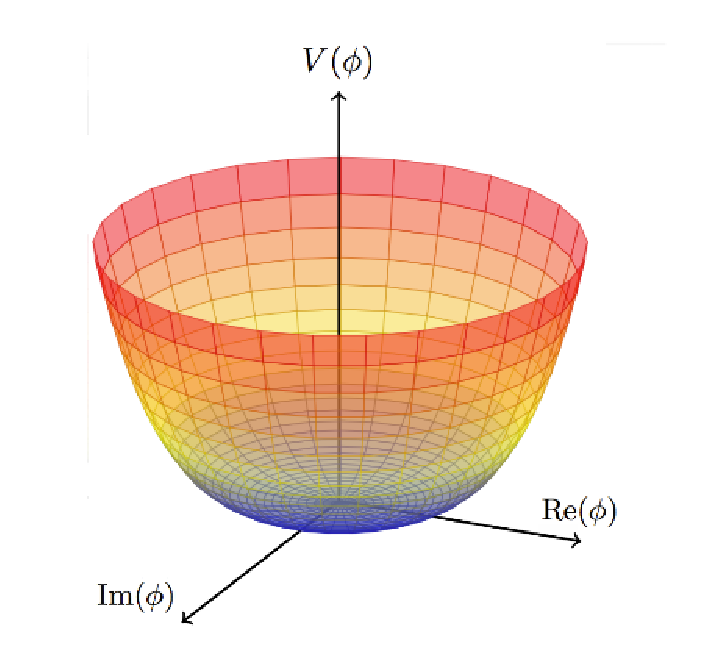
\includegraphics[width=\textwidth]{Theory/Figures/higgs1}
  \caption{}
   \end{subfigure}
   \begin{subfigure}{0.47\textwidth}
  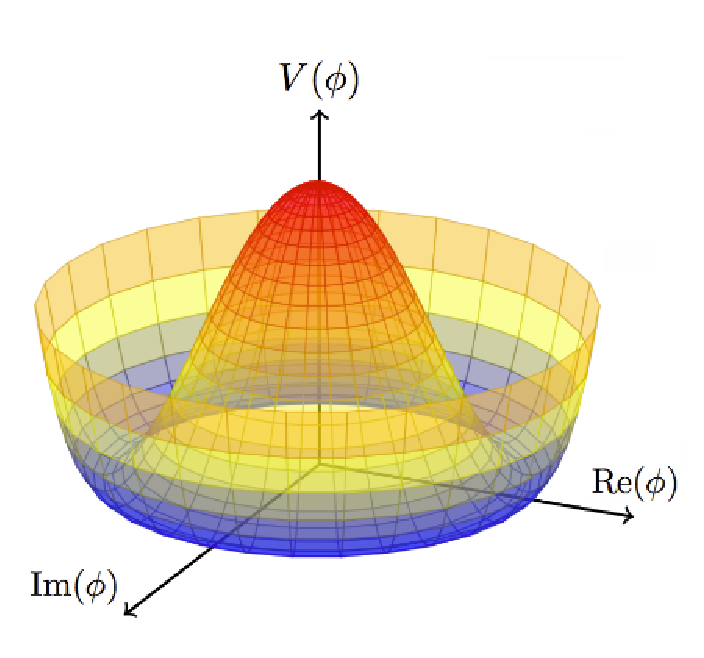
\includegraphics[width=0.9\textwidth]{Theory/Figures/higgs2}
  \caption{}
   \end{subfigure}
  \caption{Vacuum potential for $\lambda > 0$ and $\mu^2 > 0$ (a) or $\mu^2 < 0$ (b), with the typical shape of a Mexican hat.}
  \label{fig:Higgs_potential}
\end{figure}
The potential $V(\Phi)$ depends on two parameters, $\mu^2$ and $\lambda$. The case $\lambda < 0$ is unphysical, leading to no stable minima. For $\lambda > 0$, two possibilities arise: $\mu^2 > 0$ and $\mu^2 < 0$, which are illustrated in figure~\ref{fig:Higgs_potential}. In the first case there is a single solution to the minimization which corresponds to $|\Phi| =0$ and gives as vacuum expectation value (VEV), $\langle\Phi\rangle_0 \equiv \langle0|\Phi|0\rangle = 0$.
If $\lambda>0$ and $\mu^2<0$, the minimum of the potential $V(\Phi)$ is found in:

\begin{equation}
  \Phi^{\dagger} \Phi = -\frac{\mu^2}{2\lambda} \equiv \frac{v^2}{2}~,
  \label{eq:HiggsMinimumOfPotential}
\end{equation}
and therefore the field $\Phi$ has a non-zero vacuum expectation value $\langle\Phi\rangle_0 \equiv \langle0|\Phi|0\rangle = \frac{v}{\sqrt{2}}$, and there is no unique minimum. The fundamental vacuum state is no more invariant under $SU(2)_L \otimes U(1)_Y$, meaning that these two symmetries are now broken.

The Goldstone theorem states that massless scalars, referred to as Goldstone bosons, occur whenever a continuous symmetry is broken~\cite{PhysRev.127.965}.
They can be absorbed by a gauge field as a longitudinal polarization component and the gauge field acquires mass.
Since the photon is the only electroweak boson known to be massless, the minimum of the potential is chosen so that the Higgs field that acquires a VEV is the one with zero electric charge:

\begin{equation}
  \Phi_0 \equiv \frac{1}{\sqrt{2}} \left(
  \begin{matrix}
    0 \\
    v
  \end{matrix}
  \right).
  \label{eq:VEVdefinition}
\end{equation}
Expanding the field around the true minimum of the theory, the complex field $\Phi$ becomes:

\begin{equation}
  \Phi(x) = 
%e^{i\frac{\vec{\sigma}\cdot\vec{\xi}(x)}{2}} \, 
  \frac{1}{\sqrt{2}} \left(
  \begin{matrix}
    0 \\
    v + H(x)
  \end{matrix}
  \right),
  \label{eq:HiggsField}
\end{equation}
where $H(x)$ represents ground state fluctuations around the vacuum state in the direction perpendicular to the degenerate minima.
%where the three parameters $\vec{\xi}(x)$ correspond to the motion through the degenerated minima in the space, which can be set to zero ($\vec{\xi}(x)=0$) due to the gauge invariance of the lagrangian.

Additionally, nothing prevents the Higgs doublet to couple to the fermion fields.
Therefore, the interaction between the Higgs doublet and the fermion fields can be added, in the form of the Yukawa lagrangian:

\begin{equation}
  \lagrangian_{Y} = \sum_{f=l,q}{y_f \left[ \bar{f}_L \Phi f_R + \bar{f}_R \bar{\Phi}f_L \right]}~,
  \label{eq:HiggsYukawaLagrangian}
\end{equation}

\noindent where the matrices $y_f$ describe the Yukawa couplings between the Higgs doublet and the fermions.
The Yukawa lagrangian is gauge invariant since the combinations $\bar{f}_L \Phi f_R$ and $\bar{f}_R \bar{\Phi} f_L$ are $SU(2)_L$ singlets.

By introducing the expansion from equation \ref{eq:HiggsField} in the Yukawa lagrangian in equation \ref{eq:HiggsYukawaLagrangian}, the tree level predictions for the mass of the fermions can be obtained:

\begin{equation}
  m_f = y_f \frac{v}{\sqrt{2}}~,
  \label{eq:HiggsFermionMasses}
\end{equation}

\noindent where $f$ stands for the fermions of the theory.
On the other hand, the tree level mass of the Higgs boson can be computed from the Higgs lagrangian in equation \ref{eq:HiggsLagrangian}, and it is found to be:

\begin{equation}
  m_H = \sqrt{-2\mu^2} = \sqrt{2\lambda} v~.
  \label{eq:HiggsHiggsMass}
\end{equation}

Since the value of $\lambda$ is unknown, $m_H$ is not predicted by the theory and must be determined experimentally.

From the same Higgs lagrangian, the electroweak boson masses can also be obtained.
The relevant term in equation \ref{eq:HiggsLagrangian} is:

\begin{equation}
  \begin{split}
    & \left|\left(-ig\frac{\sigma}{2}\vec{W}_\mu - i\frac{g'}{2}B_\mu \right)\Phi\right|^2 \\
    &= \frac{1}{8} \left|\left(
    \begin{matrix}
      gW_\mu^3 + g'B_\mu & g(W_\mu^1 - iW_\mu^2) \\
      g(W_\mu^1 + iW_\mu^2) & -gW_\mu^3 + g'B_\mu 
    \end{matrix}
    \right)
    \left(
    \begin{matrix}
      0 \\%
      v   \
    \end{matrix}
    \right) \right|^2 \\
    &= \frac{1}{8} v^2 g^2 \left[(W_\mu^1)^2 + (W_\mu^2)^2\right] + \frac{1}{8} v^2 (g'B_\mu - gW_\mu^3)(g'B^\mu - gW^{3\mu}) \\
    &= \left(\frac{1}{2}vg\right)^2 W_\mu^{+} W^{-\mu} + \frac{1}{8} v^2 \left(W_\mu^3, B_\mu\right) 
    \left(
    \begin{matrix}
      g^2 & -gg' \\
      -gg' & g'^2
    \end{matrix}
    \right)
    \left(
    \begin{matrix}
      W_\mu^3 \\
      B_\mu
    \end{matrix}
    \right),
  \end{split}
  \label{eq:HiggsBosonMassDemonstration}
\end{equation}

\noindent defining $W^{\pm} = (W^1 \mp iW^2)/\sqrt{2}$.
The mass eigenstates can be obtained diagonalizing the mass matrix, and expressed as a function of $W_\mu^3$ and $B_\mu$:
%
%\begin{align}
%    \frac{1}{8}v^2\left[g^2\left(W_\mu^3\right)^2 - 2gg'W_\mu^3 B^\mu + g'^2B_\mu^2\right] 
%    =\ & \frac{1}{8}v^2\left[ gW_\mu^3 - g'B_\mu\right]^2           \\
%    &+ 0 \left[g'W_\mu^3 + gB_\mu\right]^2 \\
%    =\ & \frac{1}{2}\left(v\frac{\sqrt{g^2+g'^2}}2\right)^2 Z_\mu^2 & \\
%    &+ 0 \cdot A_\mu^2~, 
%  \label{eq:HiggsBosonMassDemonstration2}
%\end{align}
%
\begin{equation}
\begin{split}
    \frac{1}{8}v^2\left[g^2\left(W_\mu^3\right)^2 - 2gg'W_\mu^3 B^\mu + g'^2B_\mu^2\right] 
    =\ & \frac{1}{8}v^2\left[ gW_\mu^3 - g'B_\mu\right]^2           \\
    &+ 0 \left[g'W_\mu^3 + gB_\mu\right]^2 \\
    =\ & \frac{1}{2}\left(v\frac{\sqrt{g^2+g'^2}}2\right)^2 Z_\mu^2 \\
    &+ 0 \cdot A_\mu^2~, 
\end{split}
  \label{eq:HiggsBosonMassDemonstration2}
\end{equation}

\noindent where:

\begin{equation}
  Z_\mu = \frac{gW_\mu^3 - g'B_\mu}{\sqrt{g^2 + g'^2}}
  \label{eq:HiggsZdefinition}
\end{equation}
\begin{equation}
  A_\mu = \frac{g'W_\mu^3 + gB_\mu}{\sqrt{g^2 + g'^2}}~,
  \label{eq:HiggsAdefinition}
\end{equation}
represent the fields associated with the $Z$ boson and the photon respectively.

From equations \ref{eq:HiggsBosonMassDemonstration} and \ref{eq:HiggsBosonMassDemonstration2}, the tree level predictions for masses of the gauge bosons are:

\begin{align*}
  m_W &= \frac{vg}{2}, \\
  m_Z &= v \frac{\sqrt{g^2 + g'^2}}{2}, \\
  m_\gamma &= \unit[0]{.}
\end{align*}
%
%%\noindent By knowing that the electric charge of the photon is 0, the Nijijima equation bla bla bla can be cross-chequed.
%Finally, the Gell-Mann Nishijima formula shown in equation \ref{eq:ElectricChargeDefinition} can be validated with the boson definitions:
%
%\begin{equation}
%  \begin{split}
%    \hat{Q}A_\mu &= 0 \\
%    \hat{Q}Z_\mu &= 0 \\
%    \hat{Q}W^{\pm}_\mu &= \pm 1
%  \end{split}
%  \label{eq:ValidationElectricChargeDefinition}
%\end{equation}

\subsection{Quantum Chromodynamics}
\label{subsec:QCDtheory}

Quantum Chromodynamics (QCD) describes the strong interactions in the SM, being $SU(3)_C$  the underlying symmetry.
%responsible for the behavior of quarks being held together by the strong force, carried by gluons.
%The ``color'' group $SU(3)_C$ is the starting global symmetry.
A new quantum number, color, is introduced to refer to three different possible states of the quarks. % and it constitutes an exact symmetry of the theory.
The global gauge symmetry is promoted to a local one by introducing the covariant derivative:

\begin{equation}
  D_\mu \equiv \partial_\mu - ig_s T_a G_\mu^a~,
  \label{eq:QCDCovariantDerivative}
\end{equation}

\noindent where $g_s$ is the strong coupling constant (usually referred as $\alpha_s\equiv g_s^2 / 4\pi$ in the literature), $T_a$ are the $SU(3)_C$ generators with $a=1,\ldots,8$, and $G_\mu^a$ are the gluon fields.
After introducing the covariant derivative and a kinematic term for the gluon fields, the lagrangian of QCD is given by:

\begin{equation}
  \lagrangian_{\text{QCD}} = \bar{q}\left( i\gamma^\mu D_\mu\right) q - \frac{1}{4}G^{a}_{\mu\nu}G^{a\,\mu\nu}~,
  \label{eq:QCDlagrangian}
\end{equation}

\noindent where $\gamma^{\mu}$ are the Dirac $\gamma$-matrices and $q$ is a vector of three components corresponding to the different colors of a given quark type.
Gluons transform under the adjoint representation, while quarks are in the fundamental representation of the $SU(3)_C$ group.
The interactions between quarks and gluons are enclosed in the definition of the covariant derivative in equation \ref{eq:QCDCovariantDerivative}.
The field tensor $G^{a}_{\mu\nu}$ is given by:

\begin{equation}
  G^{a}_{\mu\nu} = \partial_{\mu}G_{\nu}^{a} - \partial_{\nu}G_{\mu}^{a} - g_s f_{abc}G_{\mu}^{b}G_{\nu}^{c}~,
  \label{eq:fieldTensorQCD}
\end{equation}

\noindent where $ f_{abc}$ are the structure constants of the $SU(3)$ group.
The third term of the tensor describes the gluon self-interaction and is responsible for the non-abelian nature of QCD.

The presence of this self-interaction induces very particular features in the dependence of the strong coupling constant with the scale of the interaction, which is shown in figure~\ref{fig:alphaRunning}. 
%The scaling of \alphas\ with $Q$ is referred to as ``running '' of the coupling constant.
\begin{figure}[tbh]
  \begin{center}
    \mbox{
      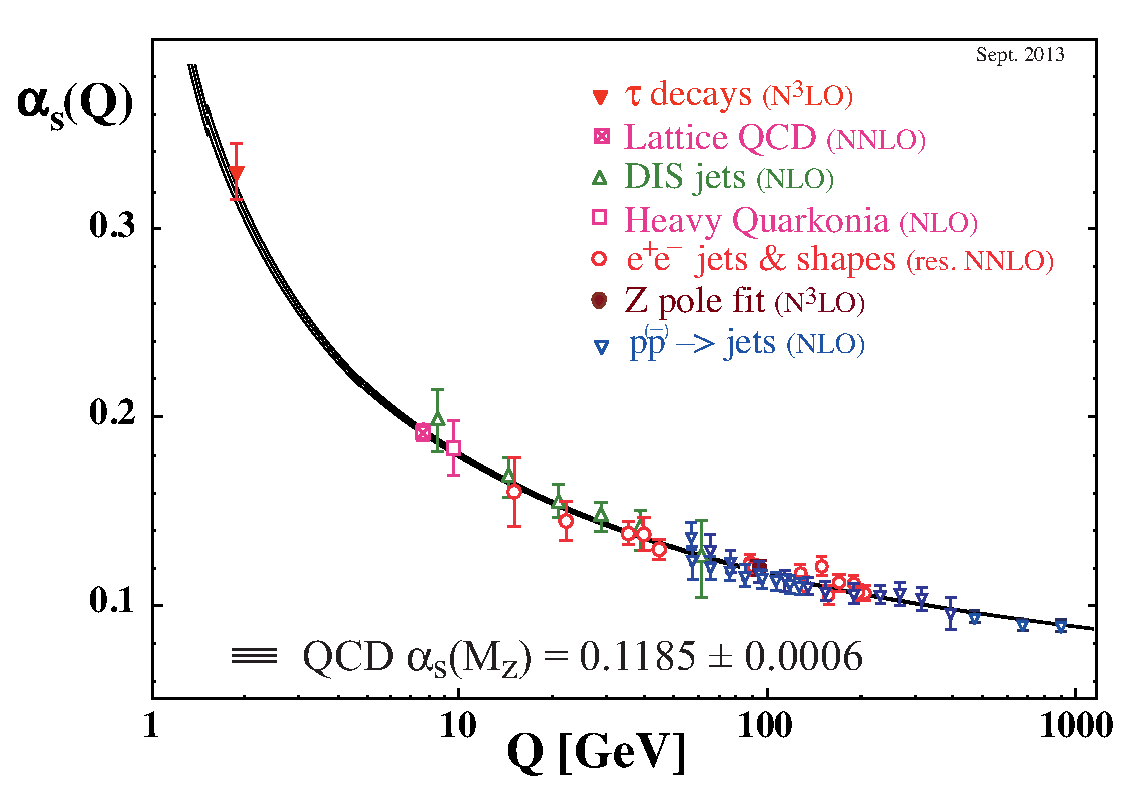
\includegraphics[width=0.7\textwidth]{Theory/Figures/asq-2013.eps}
    }
  \end{center}
  \caption{Summary of measurements of $\alpha_s$ as a function of the energy scale $Q$~\cite{Bethke:2012jm}.}
  \label{fig:alphaRunning}
\end{figure}
In the leading-order approximation~\cite{Aitchison:2004cs} the coupling constant can be expressed as:
\begin{equation}
  \alphas(Q^2)=\frac{12\pi}{(33-2n_f)\cdot \log(\frac{Q^2}{\Lambda^2_{QCD}})}~,
  \label{eq:alpha_QCD}
\end{equation}
where $n_f$ is the number of ``active flavor'' quarks (i.e. with $m_q<Q$), and $\Lambda_{QCD}$ is an infrared cut-off scale where the perturbative approximation is no longer valid. 

From equation~\ref{eq:alpha_QCD} two of the key features of QCD are derived. In the high energy regime, \alphas\ is sufficiently small that observables can be computed using perturbation theory, which gives very good mathematical properties and predictive power to the theory. Since the coupling vanishes for $Q^2 \rightarrow \infty$, in the high energy limit the quarks can propagate as if they were free, a property known as \textit{asymptotic freedom}. 
On the other hand, at low energies \alphas\ increases, to the point of diverging. This property is known as \textit{confinement}: quarks and gluons can not appear as free particles. 
When partons with colour charge start to separate from each other, the potential energy increases to a point when it becomes energetically preferable to create a quark-antiquark pair with opposite colour charge from the vacuum. This property has the experimental consequence that coloured partons  produced in high-energy interactions will manifest themselves as collimated streams of hadrons referred to as ``jets''. The process through which a quark evolves into a jet is addressed in more detail in section~\ref{subsec:HadronizationModels}.

\subsection{Experimental successes of the Standard Model}
Throughout the years the SM has been tested in multiple experiments, and its validity has been confirmed with precision measurements, sometimes with a precision better than \unit[0.1]{\%}. Since its formulation in the 70's, the SM has been able to describe accurately most experimental observations and all the discovered particles have been accommodated nicely into the model.

%The first breakthrough was the observation at CERN of the neutral current processes, compatible with a $Z$ boson~\cite{weakCurrent}.
The existence of the charm quark was predicted in order to explain the absence of flavor-changing neutral currents~\cite{PhysRevD.2.1285} and was later discovered simultaneously by groups at SLAC~\cite{PhysRevLett.33.1406} and MIT~\cite{PhysRevLett.33.1404} in what became the start of the \textit{November revolution}. 
Subsequently, the bottom quark~\cite{Herb:1977ek}, the $\tau$ lepton~\cite{Perl:1975bf} and its respective neutrino~\cite{Kodama:2000mp}, found a natural placement as a third generation of fermions.
The discovery of a third quark family provided a natural mechanism for CP violation through the complex phase of the CKM matrix~\cite{ckm}. %and this was confirmed (already seen?) in K/D/B? oscillations. CKM in 1973, CP violation in kaon oscillation in 1964.
The vector gauge bosons, $W$ and $Z$, were discovered at the CERN $Sp\bar{p}S$ collider in 1983~\cite{Arnison:1983rp}.

In 1989 experiments started at LEP, with $\eebar$ collisions at $\sqrt{s} \sim M_Z$ (LEP1) and with an increasing energy of $\sqrt{s} = 161 - 207$, in the later years (LEP2). The SM was thoroughly scrutinized with precision measurements of the $W$ and $Z$ bosons. The combination of precision measurements and theoretical calculations of radiative corrections allowed also to extract indirect constraints on the missing pieces of the SM, such as the top quark which had not been discovered. The top quark mass was precisely predicted from radiative corrections to the $W$ boson mass and the $Z\rightarrow\bbbar$ branching ratio, and was discovered in 1995~\cite{topdisc_cdf,topdisc_d0} at the Tevatron.

The consistency of the SM with the set of precision measurements was also confirmed through the \textit{electroweak fit}. The fundamental parameters of the SM can be fitted to different data measurements and it was confirmed that all the observations can be explained simultaneously from the SM predictions.
Figure~\ref{fig:gfitter_pulls} shows the differences between the predicted and the measured quantities for several observables as obtained by the Gfitter Collaboration~\cite{Baak:2013ppa}. A good consistency between measured and expected quantities is found and none of differences exceeds three standard deviations. From this fit, the mass of the Higgs boson was predicted to be $\unit[94.1^{+25}_{-22}]{\gev}$ as shown in figure~\ref{fig:gfitter_higgs}.
%\begin{wrapfigure}{r}{0.30\textwidth}
%  \centering
%  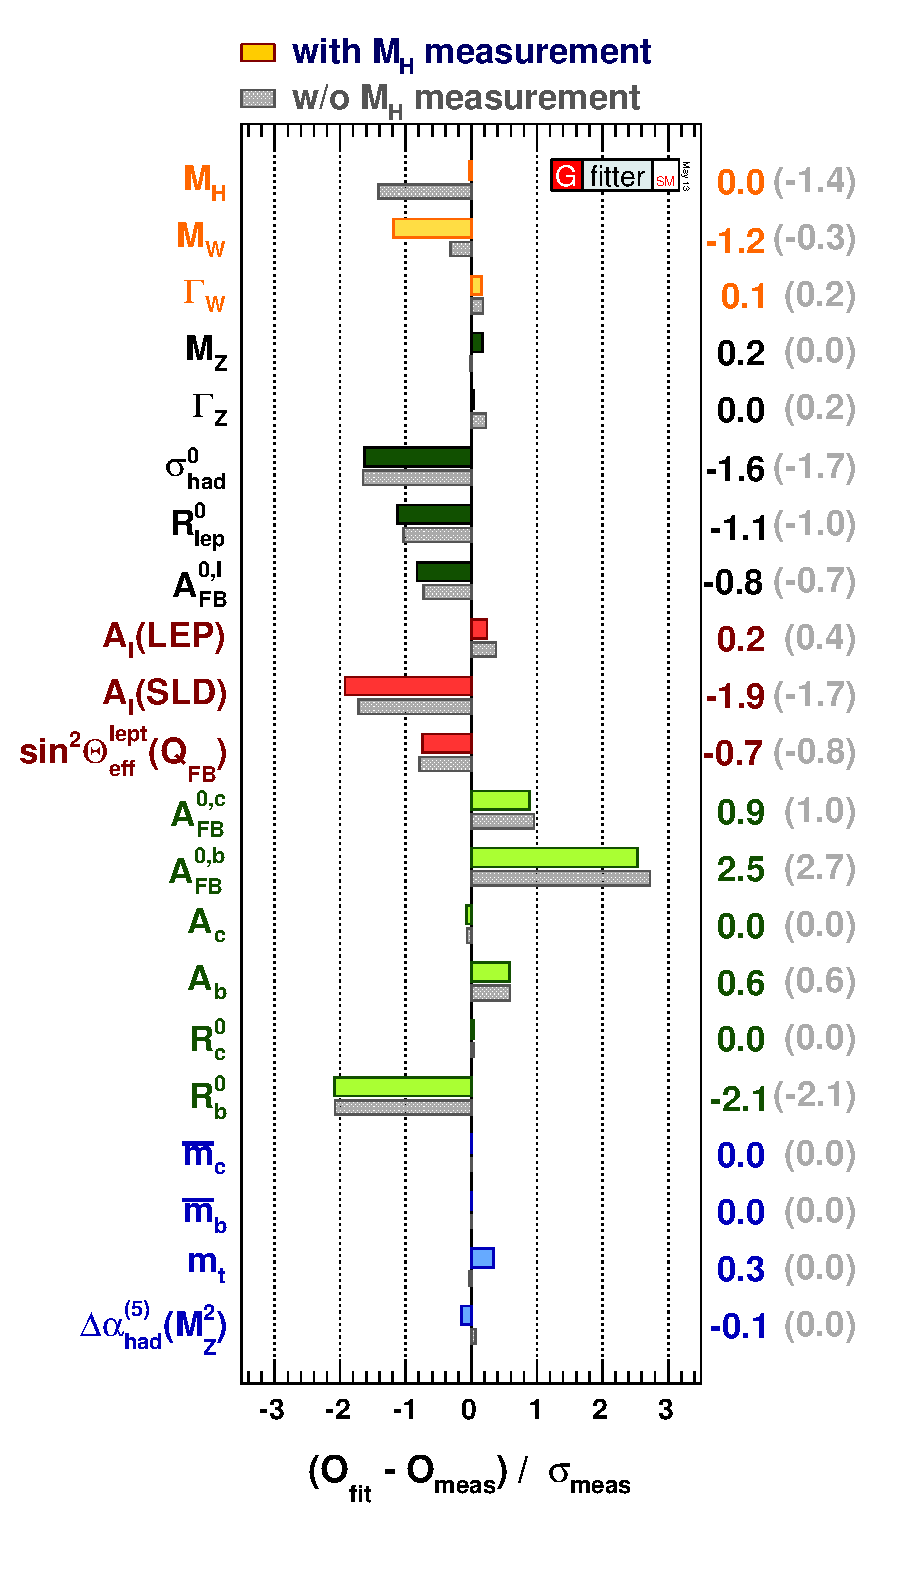
\includegraphics[width=0.7\textwidth]{Theory/Figures/2013_05_29_PullPlotTwoBarsCol_logo.eps}
%  \caption{Gfitter}
%  \label{fig:gfitter_pulls}
%\end{wrapfigure}
\begin{figure}[t!]
  \centering
        \begin{subfigure}{0.39\textwidth}
  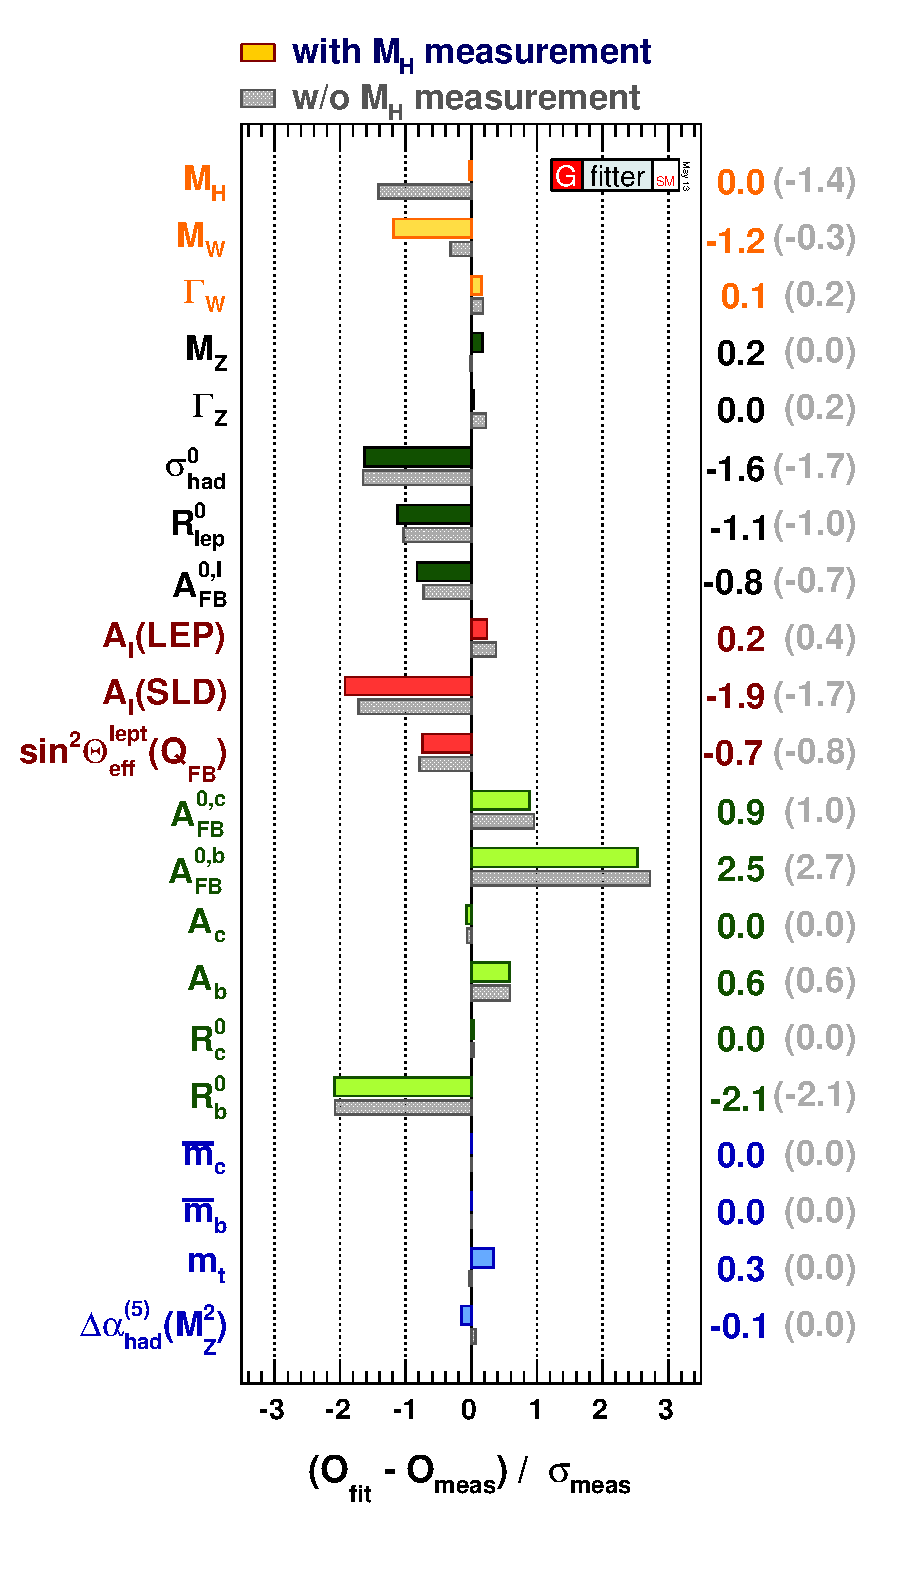
\includegraphics[width=\textwidth]{Theory/Figures/2013_05_29_PullPlotTwoBarsCol_logo.eps}
     \caption{}
  \label{fig:gfitter_pulls}
     \end{subfigure}
     \begin{subfigure}{0.6\textwidth}
    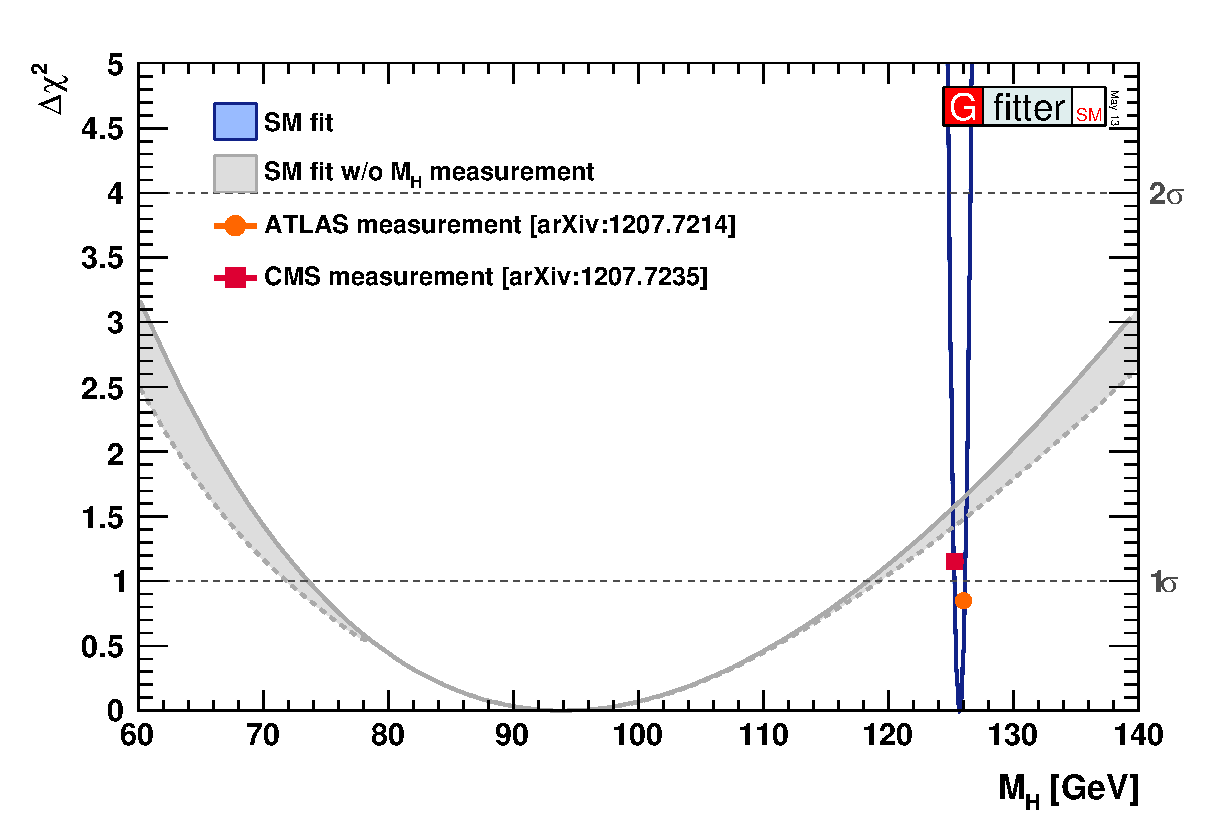
\includegraphics[width=\textwidth]{Theory/Figures/2013_05_29_HiggsScan_logo.eps}
     \caption{}
  \label{fig:gfitter_higgs}
     \end{subfigure}
  \caption{
    Left: pull values for the SM fit with and without inclusion of $M_H$ in the fit. The pull values are defined as deviations between experimental measurements and theoretical calculations in units of the experimental uncertainty.  
    Right: $\Delta \chi^2$ as a function of Higgs boson mass $M_H$, with (blue band) and without the $M_H$ measurements (gray band).
}
  \label{fig:gfitter}
\end{figure}

%\begin{figure}[t!]
%  \centering
%  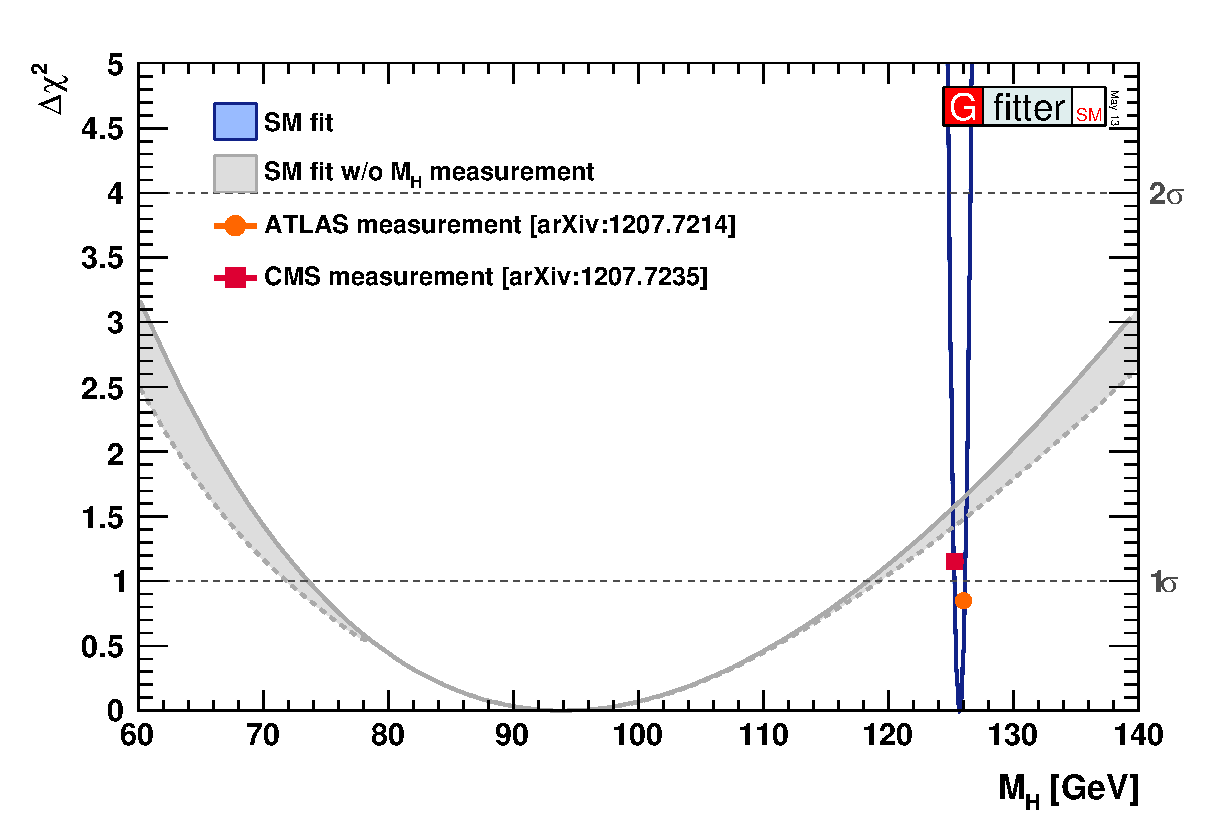
\includegraphics[width=0.7\textwidth]{Theory/Figures/2013_05_29_HiggsScan_logo.eps}
%  \caption{Gfitter}
%  \label{fig:gfitter_higgs}
%\end{figure}

The last missing piece of the SM was found in 2012, when both the ATLAS and CMS collaborations announced the observation of a new particle compatible with the Higgs boson hypothesis~\cite{Aad:2012tfa,Chatrchyan:2012ufa}.
The mass of the new particle was found to be $\unit[\sim 125]{\GeV}$~\cite{Aad:2015zhl}, well within the mass interval allowed by the indirect constraint of the electroweak fit.
Further measurements of the newly discovered particle confirmed that it is a scalar and a positive CP eigenstate~\cite{Aad:2013xqa}.
As of today, the couplings to the rest of the SM particles have been found to be in agreement with those of the SM Higgs boson. 

\subsection{Shortcomings of the Standard Model}
\label{subsec:shortcomings}
Despite the remarkable successes of the SM, there are a number of theoretical and experimental evidences that can not be accommodated into the framework.
This leads to the general conclusion that the SM has to be regarded as an effective theory, the low energy realization of a more complete theory that would be able to explain the whole spectrum of observations. While the detailed formulation of such ``Theory of Everything'' is not yet available, the investigation of the aspects where the SM fails to give a satisfactory answer can shed some light into the details of this more general theory.
\begin{itemize}
  \item One of the few experimental observations that are not explained by the SM are neutrino oscillations~\cite{Fukuda:1998mi}. Although neutrino masses are not measured directly, the measurement of oscillations requires that there is a mass difference between the different neutrino generations. A mass term for neutrinos is not present in the SM, although introducing right-handed neutrinos, or alternatives such as Majorana neutrinos can be accommodated.
  \item Measurements of the rotation curves of galaxies~\cite{Begeman:1991iy} and gravitational lensing led to the inference of the existence of non-luminous matter denominated \textit{dark matter} in the Universe.
    This was also verified in measurements of large-scale structures and cosmic microwave background~\cite{Larson:2010gs,Ade:2013zuv}.
    Dark matter doesn't interact through the electromagnetic force and therefore can not be observed, but its presence is made evident through gravitational effects. The SM has no candidate particle that can account for the large measured fraction of dark matter, encompassing more than \unit[80]{\%} of the total matter in the universe.
  \item %At the moment of the Big Bang, matter and antimmater should have been produced in the same amount, however there is a clear asymmetry and matter remains. 
    The SM can not fully explain the matter/anti-matter asymmetry observed in the Universe. Although CP-violation is described by the presence of a phase in the CKM matrix, the amount of CP-violation is not big enough as to explain the current asymmetry.
  \item The SM has 19 arbitrary parameters, out of them 9 fermion masses. The hierarchical mass structure of the SM fermions, 
    %shown in figure~\ref{fig:particle_masses}
    ranging from $\sim\unit[1]{\mev}$ for the first generation of fermions,\footnote{If neutrino masses are considered, for which the current bounds are $\sim$ eV, this difference increases by six more orders of magnitude. } to about \unit[173]{\gev} of the top quark, is not understood. Also the question of why exactly three families of fermions exist has no justification. 
    The arbitrariety of parameters in the SM, and in particular of the fermion masses, introduces the \textit{naturalness} problem. A ``natural'' theory is characterized by free parameters with values of the same order of magnitude. This does not happen in the SM, where the difference in masses spans five orders of magnitude.
    This is not a problem to the theory itself, but such huge differences in arbitrary parameters are usually considered as unnatural and a possible indication of unknown principles underlying a more complete theory encompassing the SM.
%    \begin{figure}[bh!]
%      \centering
%      \includegraphics[width=0.5\textwidth]{Theory/Figures/particle_masses.png}
%      \caption{Masses}
%      \label{fig:particle_masses}
%    \end{figure}
%    Other shortcomings of the SM are not at the fundamental level but rather unsettling observations that may point to the existence of a theory that extends the SM in order to describe the physics at higher energies. 
  \item A very important missing piece towards a Theory of Everything is the introduction of a quantum field theory for gravity. At energies of the order of the Planck scale, 
    ${M_P = \left(8\pi G_\text{Newton}\right)^{-1/2} = \unit[10^{18}]{\gev}}$, 
      %{$M_P = \left(8\pi G_\text{Newton}\right)^{-1/2} = \unit[2.4\times 10^{18}]{GeV}$}, 
    quantum gravitational effects are not negligible and a new model should replace the SM. In the hypothetical absence of new physics below this scale, the requirement that the SM has to be valid up to the Planck scale introduces a new problem known as the ``hierarchy problem''.
\end{itemize}

\subsubsection{The hierarchy problem} 
A further argument pointing to the need for new theories beyond the SM is the ``hierarchy problem'', which can be defined as the fact that the difference between the weak scale and the Planck scale, $M_P/M_W$, is so huge.
This is not a fundamental problem of the SM itself, but it introduces a disturbing sensitivity of the Higgs potential to new physics in almost any imaginable extension of the SM.
Unlike the fermions and gauge bosons, elementary scalars as the Higgs boson are not protected by chiral or gauge symmetries against large radiative corrections to their masses.
%In particular, in the SM there is no mechanism to prevent scalar particles from acquiring large masses through radiative corrections.
For this reason, the Higgs field receives enormous corrections from the virtual effects of any SM particle it couples to.

\begin{figure}[!t]
  \centering
   \begin{subfigure}{0.49\textwidth}
      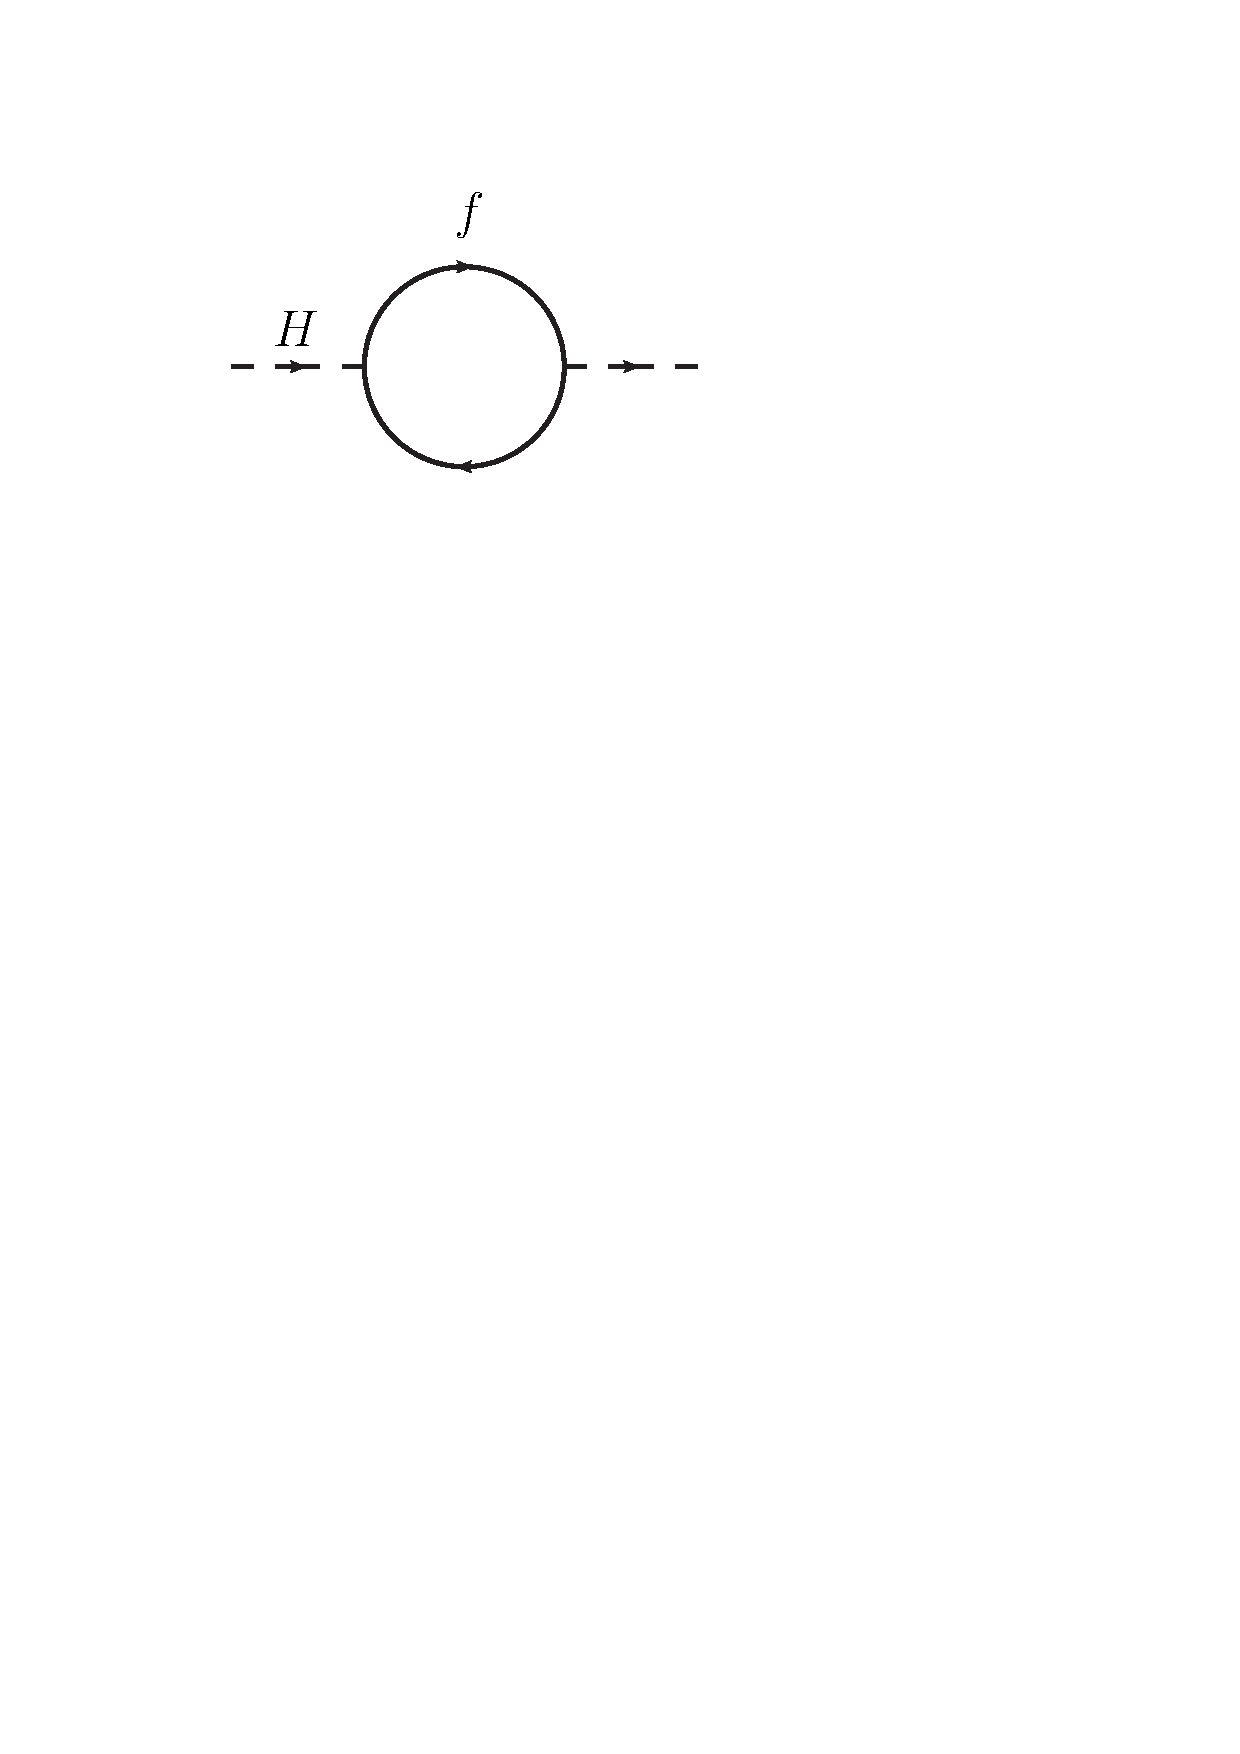
\includegraphics[width=\textwidth]{Theory/FeynmanGraphs/loopFermion.pdf}
     \caption{}
      \label{fig:loopFermion}
 \end{subfigure}
   \begin{subfigure}{0.49\textwidth}
      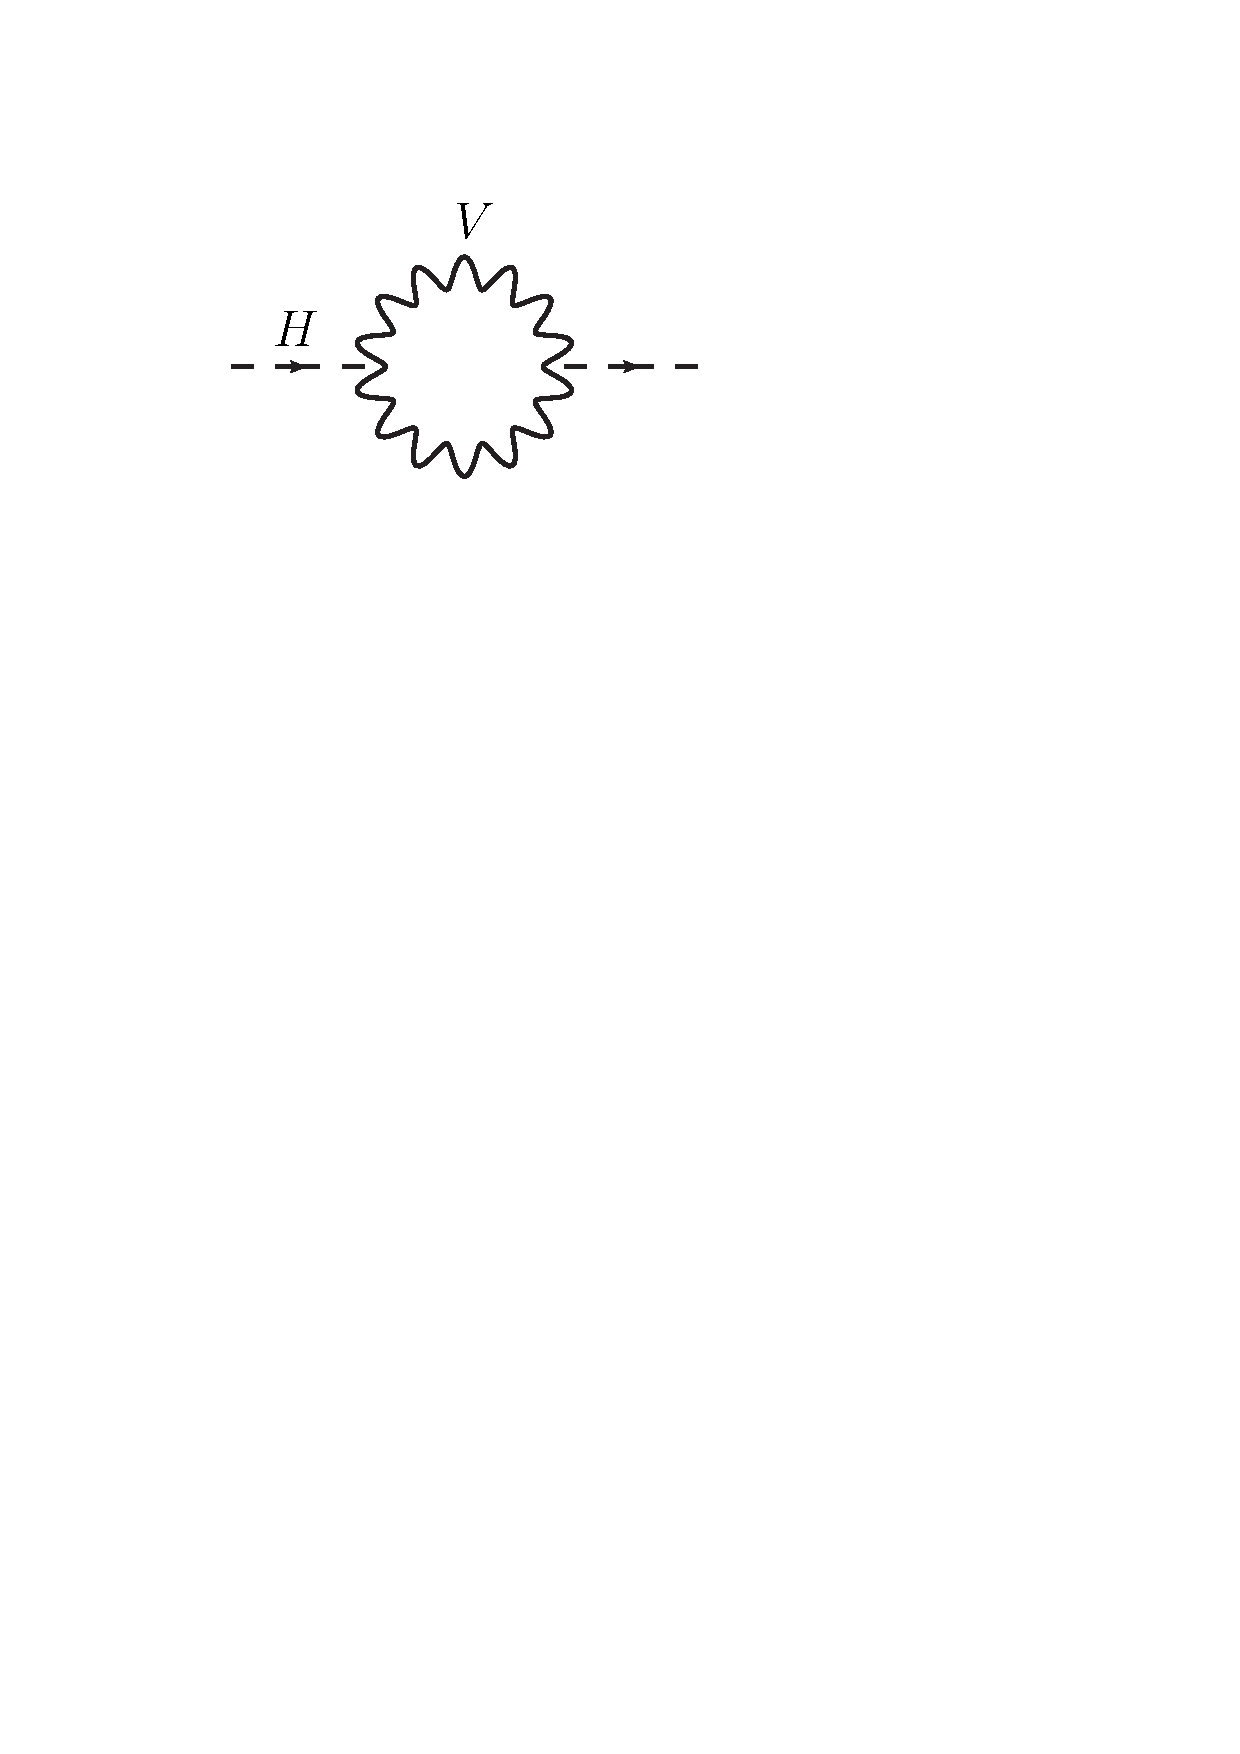
\includegraphics[width=\textwidth]{Theory/FeynmanGraphs/loopBoson.pdf}
     \caption{}
      \label{fig:loopBoson}
 \end{subfigure}
  \caption{Examples of one-loop quantum corrections to the Higgs mass due to fermions (left) and bosons (right).}
%  \label{fig:HiggsLoop}
\end{figure}

Due to these corrections, the Higgs boson mass is:

\begin{equation} 
  m_H^2 = (m_H)_{0}^{2} + \Delta m_H^2~,
  \label{eq:HiggsMassTotal}
\end{equation}

\noindent where $(m_H)_0$ is the bare Higgs mass and $\Delta m_H^2$ is the Higgs mass correction which, for the case of a fermion loop as in figure~\ref{fig:loopFermion}, is given by:

\begin{equation}
  \Delta m_H^2 = -\frac{|y_f|^2}{16\pi^2}\left[2\Lambda^2 + \mathcal{O}\left(m_f^2\ln{\left(\frac{\Lambda}{m_f}\right)}\right)\right]~,
  \label{eq:HiggsMassCorrectionFermion}
\end{equation}

\noindent being $y_f$ the Yukawa coupling of the fermion $f$ and being $\Lambda$ a cutoff.
The latter is interpreted as the energy scale at which new physics enters and the SM ceases to be valid.
Similar corrections arise also from gauge-boson loops, as shown in figure~\ref{fig:loopBoson}.
If the SM needs to describe Nature up to $M_P$, then the quantum corrections to the Higgs mass can be up to 30 orders of magnitude larger than the measured Higgs boson mass squared.
In order to recover the measured mass of the Higgs boson, the value of the bare Higgs mass and the corrections have to exactly cancel to an incredible precision. This precise cancellation is known as \emph{fine tuning}.

Since this cancellation over 16 orders of magnitude, although not forbidden, seems to be a too lucky coincidence, several extensions of the SM have been proposed where different mechanisms are present to keep the Higgs boson mass at the electroweak scale.

%\subsubsection{The top Yukawa coupling}
The largest correction to the Higgs boson mass comes from the top quark, since it is the heaviest particle in the SM. The latest Tevatron--LHC combination for the top mass yields: $m_{\mathrm{t}}=173.34 \pm 0.76 \GeV$~\cite{ATLAS:2014wva}.
This value implies that the top quark is the only particle in the SM to have a Yukawa coupling $y_{\mathrm{t}}$ very close to unity:
\begin{equation}
  y_{\mathrm{t}} = \frac{\sqrt{2}m_{\mathrm{t}}}{v} = 0.996 \pm 0.005~.
  \label{eq:top_yukawa}
\end{equation}
%It is also the particle that induces the largest radiative correction to the top mass.
While in the SM $y_{\mathrm{t}}$ is one of the free parameters of the theory, 
such particular value suggests that the top quark might have a special role in the electroweak symmetry breaking mechanism and the mass hierarchy pattern.
%At the same time, several proposed extensions of the SM predict the presence of new particles strongly coupling to the top quark.

\section{Beyond the Standard Model}
\label{sec:BSM}
Over the years, many theories have been proposed that try to extend the SM in order to solve one or several of its shortcomings. Several of these theories provide solutions for the hierarchy problem. In the following, some of these scenarios are reviewed, highlighting the phenomenology of those models predicting \ttbar\ final states with additional heavy-flavor jets, which is the signature explored in this dissertation.
\subsection{Supersymmetry}
The hierarchy problem can be solved if for each SM particle a new particle is introduced with spin differing by 1/2, that also couples to the Higgs boson. In the example of a SM fermion, a new boson $S$ is introduced, and the correction to the Higgs mass is given by:
\begin{equation}
  \Delta m_H^2 = \frac{y_S^2}{16\pi^2}\left[2\Lambda^2 + \mathcal{O}\left(m_S^2\ln{\left(\frac{\Lambda}{m_S}\right)}\right)\right],
  \label{eq:HiggsMassCorrectionScalar}
\end{equation}
where it has to be highlighted that this correction has opposite sign to the fermion contribution in equation~\ref{eq:HiggsMassCorrectionFermion}. If $y_S = |y_f|$, all the fermion terms have a counter term that naturally cancels the quadratic divergence introduced. The residual correction terms to the Higgs mass, ignoring the logarithmic contributions, would be:

\begin{equation}
  \Delta m_H^2 = \frac{y_f^2}{16\pi^2} |m_S^2 - m_f^2|~.
  \label{eq:HiggsMassCorrectionNoQuadratic}
\end{equation}

Invoking ``naturalness'' arguments, the size of the corrections is expected to be smaller than $m_{H}$, which leads to:

\begin{equation}
  |m_S^2 - m_f^2| \lesssim \unit[1]{TeV}^2~.
  \label{eq:HiggsNaturalnessCondition}
\end{equation}

This can be understood as the range of validity of the SM: at the \tev\ scale superpartners of the SM particles can be produced and the SM is replaced by its supersymmetric extension. This scale, derived from naturalness arguments, is not a strict upper bound on supersymmetric extensions, but rather a desirable scale where supersymmetry could stabilize the corrections to the Higgs mass before developing its own hierarchy problem, as discussed below.

The postulation of new particles canceling to first order all SM corrections to the Higgs mass is done through the introduction a new symmetry: supersymmetry.
In fact, supersymmetry (SUSY) seems to be the last possible extension of the Lorentz group~\cite{Haag:1974qh}.
A supersymmetry transformation turns a bosonic state into a fermionic state and viceversa~\cite{Drees:1996ca}. 
%The SM particles can then be organized into supermultiplets with their supersymmetric partners
The mass of the superpartners is predicted to be the same as the SM particles but, since no supersymmetric particle has been observed yet, supersymmetry must be a broken symmetry and supersymmetric particles' masses have to be above the reach of current experiments.

The extension of the SM through a supersymmetry is not unique: the number of generators in the symmetry group, as well as the composition and arrangement of the SM particles into supermultiplets allow many possibilities. Supersymmetry is not a fixed model but a framework from which many SM extensions can be derived. 

The minimal supersymmetric Standard Model (MSSM) is a model that introduces the minimal amount of new particles. It consists of one single operator in the symmetry group and every SM particle is paired with one single superpartner. Partners of the fermions are denoted with the prefix ``s'', for example the superpartner of the top quark is referred to as \textit{stop}, and partners of the SM bosons are labeled with the suffix ``ino''. The Higgs sector requires the introduction of an additional complex doublet, therefore producing five particles after giving mass to the SM bosons. Table~\ref{tab:MSSM_content} shows the arrangement and notation of the MSSM particle content.

\begin{table}[!ht]
  \begin{center}
    \begin{small}
      %\setlength{\tabcolsep}{0.0pc}
      %\begin{tabular*}{\textwidth}{@{\extracolsep{\fill}}ccccc}
      \begin{tabular}{ccccc}
        \toprule
        \toprule
        \textbf{Names} & \textbf{Spin} & \textbf{$P_R$} & \textbf{Gauge eigenstates}      & \textbf{Mass Eigenstates} \\
        \midrule
        Higgs bosons   & $0$           & $+1$                 & $H_u^0$ $H_d^0$ $H_u^+$ $H_d^-$ & $h^0$ $H^0$ $A^0$ $H^\pm$ \\
        \midrule
        \multirow{3}{*}{Squarks} & \multirow{3}{*}{$0$} & \multirow{3}{*}{$-1$} & $\tilde{u}_L$ $\tilde{u}_R$ $\tilde{d}_L$ $\tilde{d}_R$ & same \\
        &                      &                       & $\tilde{s}_L$ $\tilde{s}_R$ $\tilde{c}_L$ $\tilde{c}_R$ & same \\
        &                      &                       & $\tilde{t}_L$ $\tilde{t}_R$ $\tilde{b}_L$ $\tilde{b}_R$ & $\tilde{t}_1$ $\tilde{t}_2$ $\tilde{b}_1$ $\tilde{b}_2$ \\
        \midrule
        \multirow{3}{*}{Sleptons}& \multirow{3}{*}{$0$} & \multirow{3}{*}{$-1$} & $\tilde{e}_L$ $\tilde{e}_R$ $\tilde{\nu}_e$ & same \\
        &                      &                       & $\tilde{\mu}_L$ $\tilde{\mu}_R$ $\tilde{\nu}_\mu$ & same \\
        &                      &                       & $\tilde{\tau}_L$ $\tilde{\tau}_R$ $\tilde{\nu}_\tau$& $\tilde{\tau}_1$ $\tilde{\tau}_2$ $\tilde{\nu}_\tau$ \\
        \midrule
        Neutralinos    & $1/2$           & $-1$                 & $\tilde{B}^0$ $\tilde{W}^0$ $\tilde{H}_u^0$ $\tilde{H}_d^0$ & $\ninoone$ $\ninotwo$ $\ninothree$ $\ninofour$ \\
        \midrule
        Charginos      & $1/2$           & $-1$                 & $\tilde{W}^\pm$ $\tilde{H}_u^+$ $\tilde{H}_d^-$ & $\chinoonepm$ $\chinotwopm$ \\
        \midrule
        Gluino         & $1/2$           & $-1$                 & $\gluino$ & same \\
        \bottomrule
        \bottomrule
      \end{tabular}
    \end{small}
  \end{center}
  \caption[Predicted MSSM spectra.]{The predicted particle spectra in the MSSM (sfermion mixing for the first two families is assumed to be negligible).}
  \label{tab:MSSM_content}
\end{table}

The most general MSSM can contain operators that violate baryon and/or lepton number, thus allowing proton decays. The non-observation of proton decays forbids the existence of such terms.\footnote{
Strictly speaking, it imposes very stringent upper limits on the coefficients of those operators.}
A possibility to avoid these operators is to introduce a new discrete symmetry named $R$-parity. The conserved quantum number is defined as:

\begin{equation}
  P_R = (-1)^{3(B-L)+2s}~,
  \label{eq:RparityDefinition}
\end{equation}

\noindent where $B$ and $L$ refer to the baryon and lepton quantum numbers respectively and $s$ is the spin of the particle.
This definition sets all the SM particles to have $P_R = +1$ while the SUSY partners have $P_R = -1$.

\subsubsection{Supersymmetry phenomenology}
The conservation of the $R$-parity has several phenomenological consequences:

\begin{itemize}
  \item It prevents baryon and lepton quantum numbers to be violated, therefore removing terms that allow proton decay.
  \item There can be no mixing between the SM particles and their supersymmetric partners.
  \item SUSY particles can only be produced in pairs in the collisions of SM particles.
  \item The lightest SUSY particle (LSP) is stable, and therefore constitutes a good candidate for dark matter if electrically neutral.
\end{itemize}

After electroweak symmetry breaking, the supersymmetric partners mix giving rise to the mass eigenstates. 
The neutral higgsinos ($\tilde{H}_u^0$ and $\tilde{H}_d^0$) and the neutral gauginos ($\tilde{B}$ and $\tilde{W}^0$) combine to form four mass eigenstates named neutralinos.
The charged higgsinos ($\tilde{H}^+_u$ and $\tilde{H}^-_d$) and the winos ($\tilde{W}^+$ and $\tilde{W}^-$) mix to form two mass eigenstates with electric charge~$\pm 1$, named charginos.

In the sfermion sector, mixing across generations can cause large contributions to flavor changing neutral current processes~\cite{Ellis:1981ts} and is usually removed. However, mixing between the left-handed and the right-handed sfermions\footnote{
  The ``handedness'' of the scalar superpartners does not refer to their helicity, but to that of their SM partners.
}
of the same generation depends on the mass of the SM fermion, and therefore can't be neglected for the third generation superpartners.
After mixing, the mass eigenstates are labeled as $\tilde{q}_1$, $\tilde{q}_2$.

The MSSM, with the requirement of R-parity conservation, provides a solution to the hierarchy problem and contains a good candidate for dark matter. However, it also introduces 105 new parameters, to be added to the 19 parameters of the SM.
In order to reduce the number of parameters to be considered, several simplifications and assumptions are introduced in collider searches. Usually, only the sparticles that contribute to a particular final state are considered. The rest of the superpartners are considered heavy enough so that they can be completely decoupled. 
%For the analysis presented in this dissertation, only the top quark partners and the lightest neutralino, \stopone, \stoptwo, \neutralino, are considered to be kinematically accessible at the LHC.

\subsection{Extra dimensions}
The formulation of the SM assumes that our universe exists in a four-dimensional space-time. However, some theories propose that our universe is a four-dimensional ``brane'' embedded in a higher-dimensional space, referred to as ``bulk''. The effect of gravity is therefore diluted in the extra dimensions, giving an explanation for the apparent weakness of the gravitational force.
A general feature of models with extra dimensions is that particles propagating in the extra dimensions manifest in our four-dimensional brane as Kaluza-Klein (KK) states. These are a series of infinite modes, also referred to as ``towers'', where the mass of each Kaluza-Klein mode corresponds to the modulus of its momentum in the direction transverse to the four-dimensional brane.

\subsubsection{Large extra dimensions, ADD model}
In the Arkani-Hamed-Dimopoulos-Dvali (ADD) model~\cite{ArkaniHamed:1998rs}, the only particle that can propagate through the extra dimensions is the graviton, the hypothetical boson of gravity. The extra spatial dimensions are compactified with a radius $R$, on a scale which is small enough as to not have been probed yet. 
The ``effective'' four-dimensional Planck scale is equivalent to $M_P^2 \sim M_D^{2+n} R^n$, where $M_D$ is the fundamental Planck scale in $4+n$ dimensions, where $n$ is the number of extra spatial dimensions. In the ADD model, the electroweak scale $M_{EW}$ is the only fundamental short scale in nature. The equivalence $M_D \sim M_{EW}$ can be obtained for example if $n=2$ and $R \sim \unit[100]{\mu m}$.

Experimentally, the limits on the $M_D$ scale for ADD models are in the range of $\unit[3-5]{\tev}$ for $2-6$ extra dimensions~\cite{Aad:2015zva}, pushing $M_D$ away from the electroweak scale. 

\subsubsection{Universal extra dimensions}
\label{subsubsec:UED}
Other models postulate universal extra dimensions (UED)~\cite{Appelquist:2000nn}, where all SM particles can propagate in the extra dimensions. The main challenge for these theories is recovering the SM behavior after compactification of the extra dimensions. One of the options is the existence of two extra dimensions, which are compactified under the real projective plane geometry (RPP)~\cite{Burdman:2006gy,Cacciapaglia:2009pa}.

A distinctive feature of models with UED is
that each KK vector mode is accompanied by a \mbox{spin-0} particle
in the adjoint representation of the corresponding
gauge group. The partner of the gluon is a massive coloured scalar that is generically referred to as sgluon.

\subsubsection{Randall-Sundrum extra dimensions}
Another particularly interesting model is the Randall-Sundrum (RS) theory~\cite{Randall:1999vf,Contino:2006nn}. Models with extra dimensions usually rely on a factorizable geometry, namely the metric of the four familiar dimensions is independent of the coordinate in the extra dimensions. In the RS theory this assumption is dropped. The universe is considered a five-dimensional anti-de Sitter space ($\text{AdS}_5$) described by a warped geometry and the background metric solves the hierarchy problem~\cite{Randall:1999ee}. 
The background metric contains a multiplicative factor that depends exponentially on the distance to the ``gravity-brane''. The 15 orders of magnitude between the weak and the Planck scale could be explained by the distance from our brane to the gravity-brane.

\subsection{Compositeness}
Throughout the history of physics, several times a particle that was believed elementary revealed its composite nature when studied at higher energy scales. Pions, protons and even atoms were considered elementary at some point. Several new theories propose a similar situation for the SM, where particles that we consider elementary are made of yet unknown constituents which are strongly coupled through new heavy resonances.

Models of partial compositeness are also possible, where elementary and composite particles mix, and the SM particles are in fact linear combinations of elementary and composite states.

\subsubsection{Higgs boson compositeness}
The idea of a composite Higgs boson has its origin in the QCD sector where the pion mass is naturally low. In a theory with spontaneous symmetry breaking, Goldstone bosons arise as scalar, massless particles~\cite{PhysRev.127.965}. If the symmetry is not exact, and is both spontaneously and explicitly broken, then the Goldstone bosons can acquire mass. In this case the boson is called a pseudo-Goldstone boson (PGB). 
%A nice example of a pseudo-Goldstone boson is the pion, which was considered the responsible for quark masses. 
In QCD the flavor chiral symmetry of the Lagrangian is broken spontaneously, generating three massless scalar bosons. The further explicit symmetry breaking operated by the quark masses gives mass also to the pseudo-Goldstone bosons which is, however, much smaller than the other mesons' masses. The three pseudo-Goldstone bosons are the $\pi^{\pm}$ and $\pi^0$ particles, which are not elementary but composed of a quark-antiquark pair.

In a similar way, some theories propose a mechanism of strong electroweak symmetry breaking~\cite{Kaplan1984187}. A new sector is added to the SM containing the Higgs field and new strongly-interacting particles, usually named the composite sector. In the composite sector a global symmetry is spontaneously broken and then, thanks to a small mixing with the SM sector, it is also explicitly broken producing a pseudo-Goldstone boson, the Higgs boson, which is much lighter than the scale of the new sector.
In this scenario the radiative corrections to the Higgs mass don't have to reach the Planck scale since it will reveal its composite nature at the energy scale of the new strong sector.

Strongly interacting theories have usually difficulties to pass electroweak precision tests, or even to compute their contributions. Another problem of these models is explaining the origin of fermion masses.
In the past years, models of pseudo-Goldstone Higgs in the framework of a five-dimensional $\text{AdS}_5$ theory~\cite{ED1,Agashe:2004rs}
 have received increasing attention since the theory is weakly coupled, making it possible to perform calculations, and it can satisfy the bounds from electroweak data.

\subsubsection{Top quark compositeness}
Certain models propose that the top quark is not an elementary particle, but rather a composite or condensate state.
In models with composite particles due to a new strong sector, SM particles can get their masses by mixing with composite states. Given the large mass of the top quark it would be natural to expect the top quark to have a sizable admixture of the composite state and therefore to show properties of compositeness~\cite{Pomarol:2008bh,Kumar:2009vs}. Electroweak precision data strongly constrains the possibility of a composite left-handed top. Therefore, most models focus on right-handed composite top quarks~\cite{Lillie:2007hd,Georgi:1994ha}.

\section{Signatures of BSM theories}
The new particles predicted by the different theories are generally short-lived, and they can be detected by looking for their decay products. 
The analyses discussed in this dissertation explore a final state compatible with the production of a top quark pair with additional heavy-flavor jets. The different theories discussed in section~\ref{sec:BSM} can produce the targeted final state, and their phenomenology is described in the following.

\subsection{Fermionic top partners: vector-like quarks}
Several models predict the existence of vector-like quarks (VLQ), defined as color-triplet \mbox{spin-1/2} fermions whose left- and right-handed chiral components have the same transformation properties under the weak-isospin gauge group~\cite{delAguila:1982fs,AguilarSaavedra:2009es}. 
Vector-like quarks are required if the Higgs  boson is a pseudo-Goldstone boson, they also arise as KK excitations of SM quarks propagating in the bulk and in grand unified theories based on the $E_6$ group~\cite{Frampton:1999xi,Hewett1989193}.
The introduction of vector-like quarks also stabilizes the Higgs boson mass since the quadratic divergences cancel and only a logarithmic divergence remains. The one-loop contributions to the Higgs boson mass are shown in figure~\ref{fig:VLQ_loop}.

\begin{figure}[tb]
  \begin{center}
   \begin{subfigure}{0.32\textwidth}
  	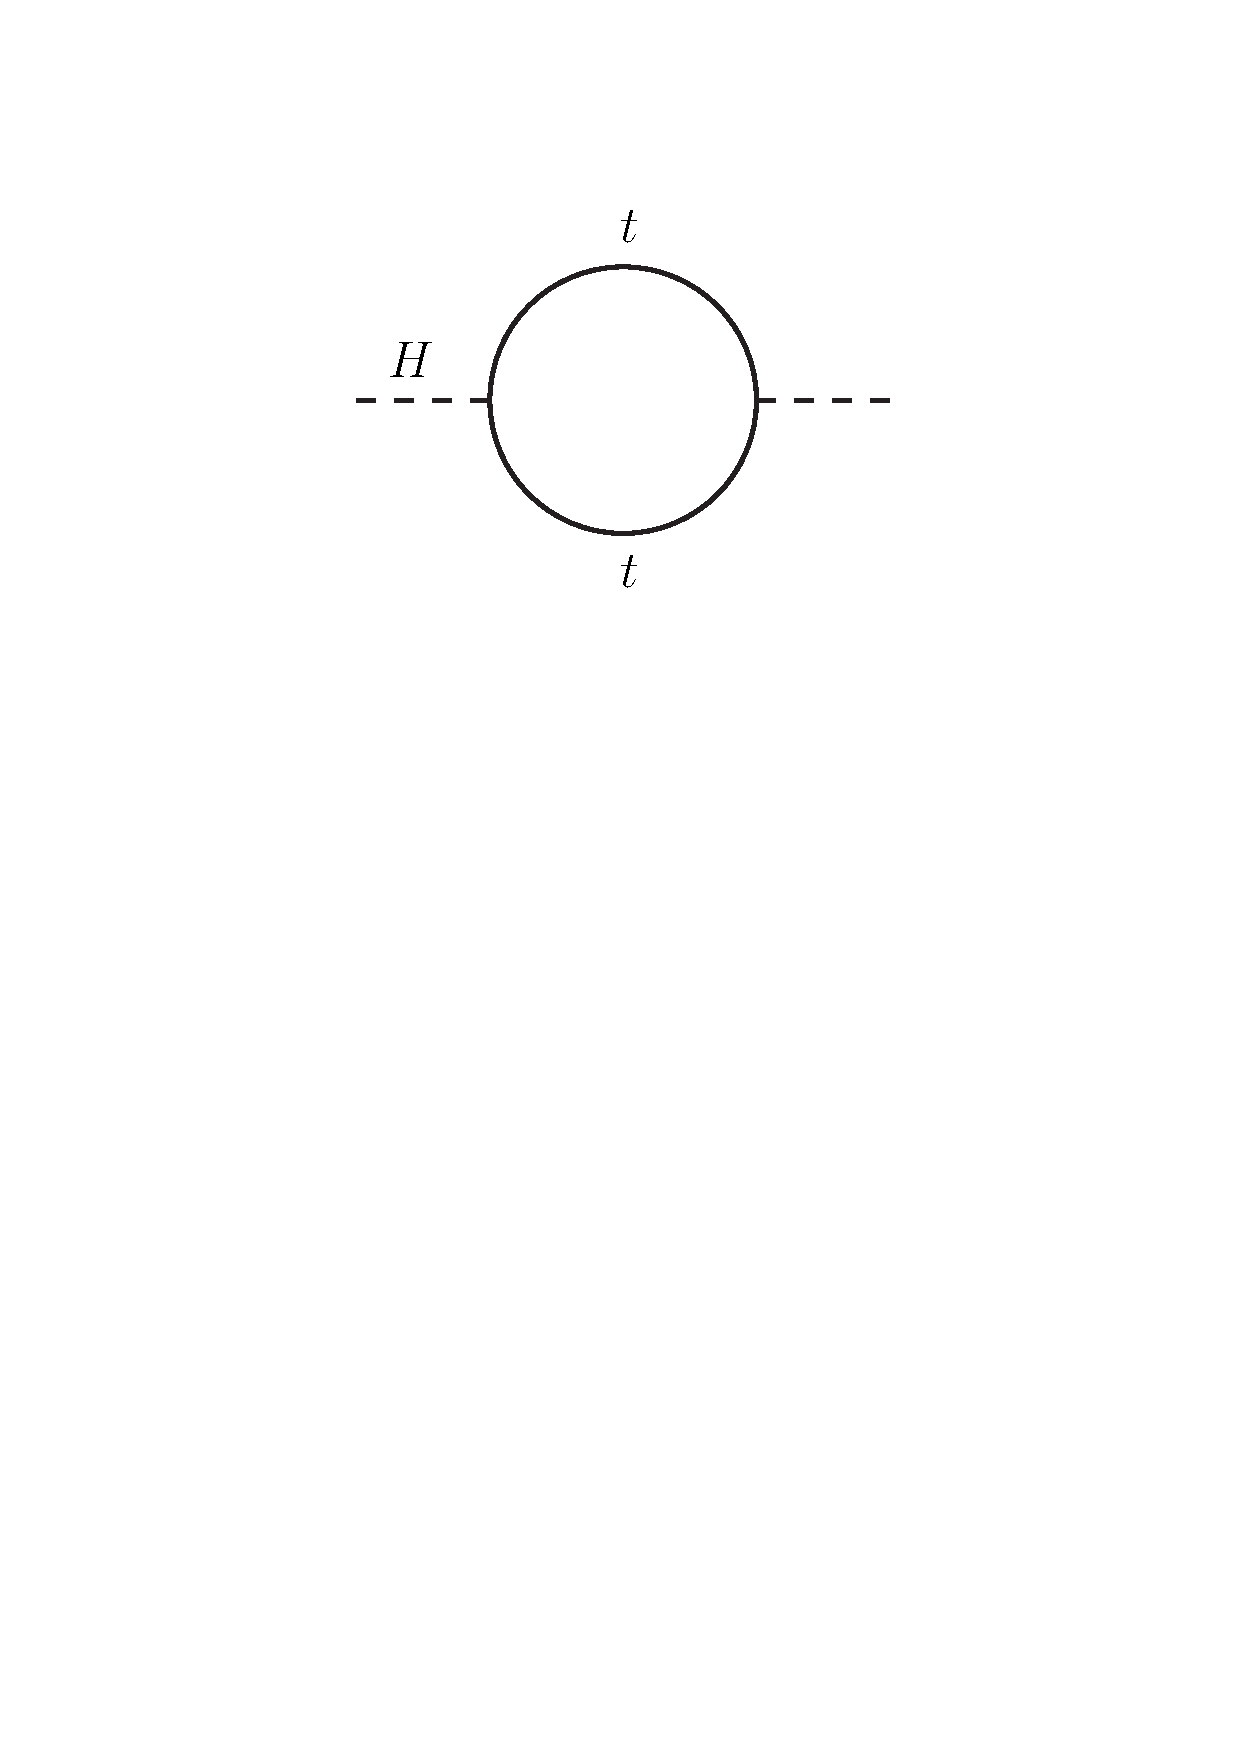
\includegraphics[width=0.92\textwidth]{Theory/FeynmanGraphs/loop_toptop_good}
    \caption{} \end{subfigure}
   \begin{subfigure}{0.32\textwidth}
  	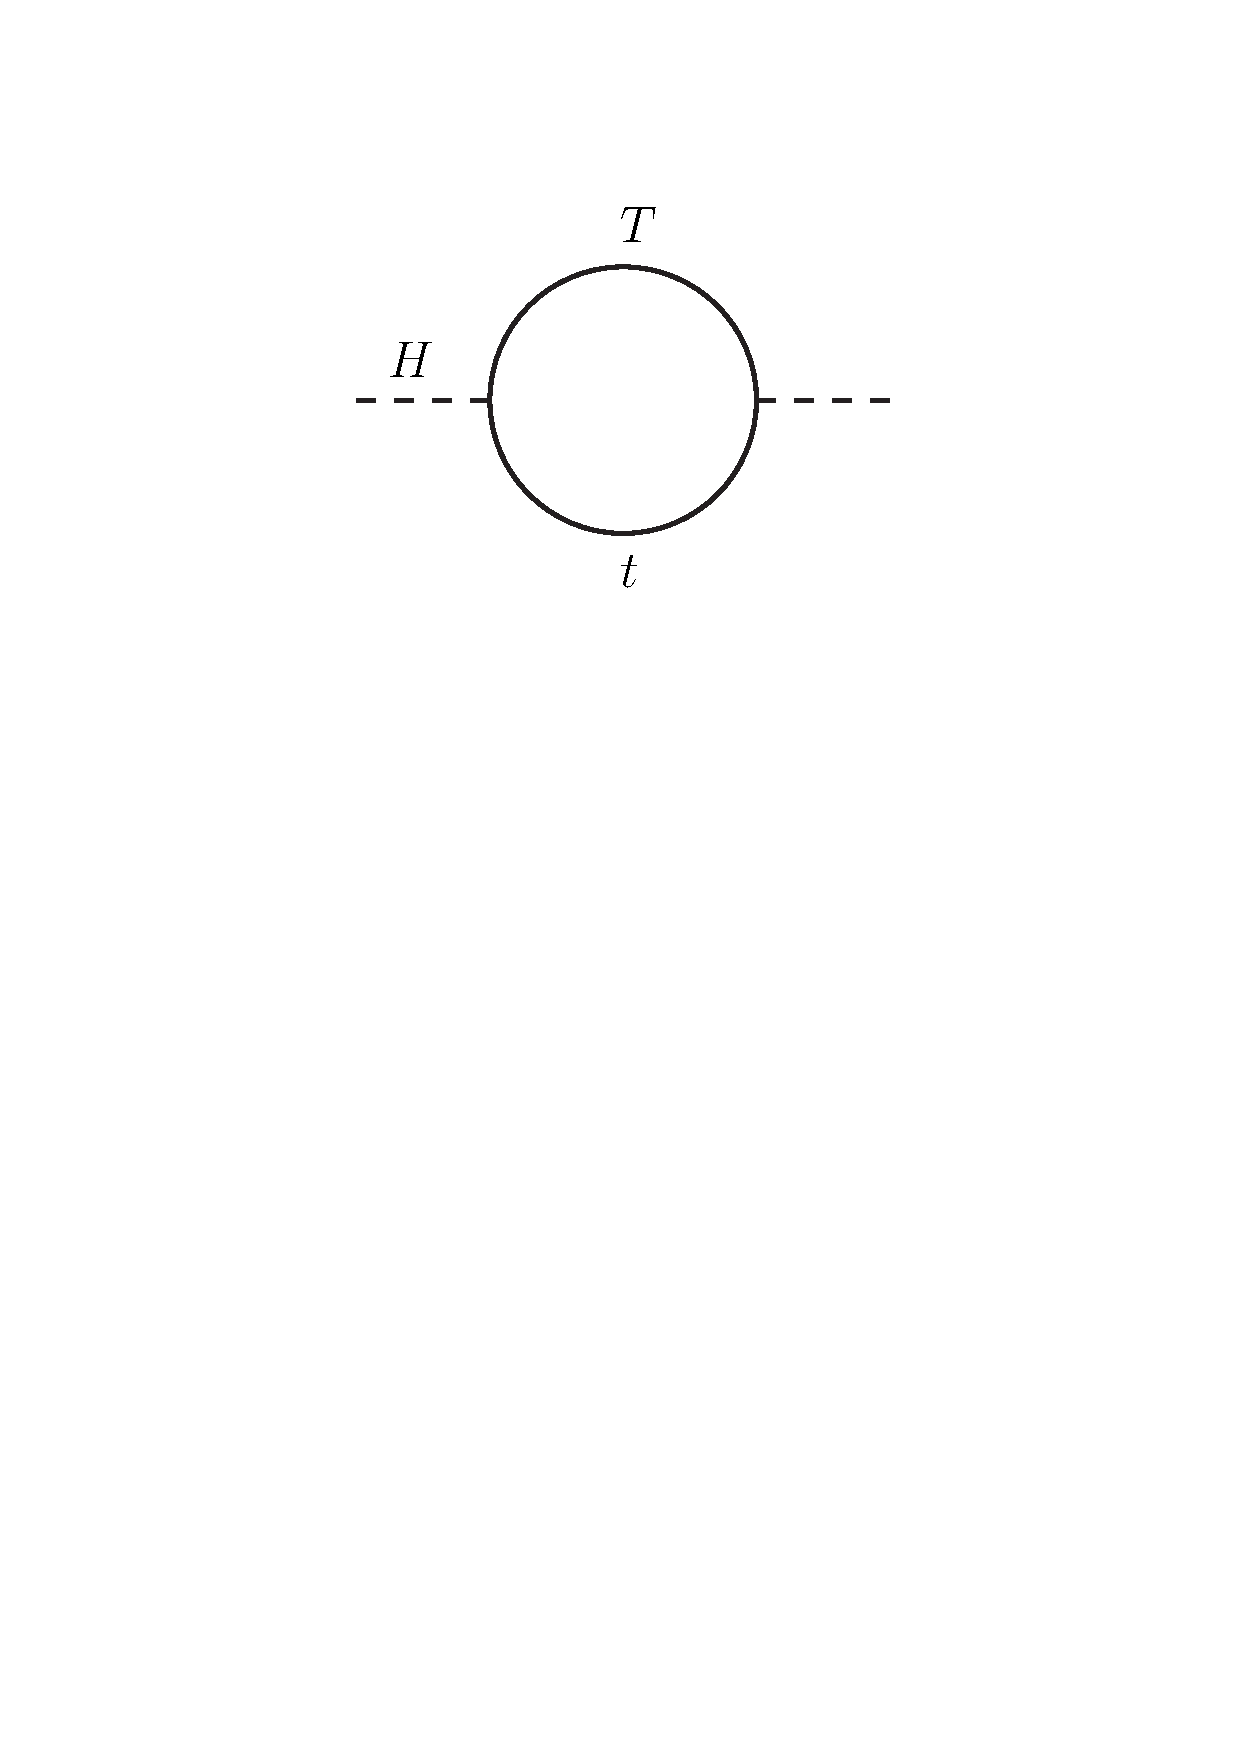
\includegraphics[width=0.92\textwidth]{Theory/FeynmanGraphs/loop_topT_good}
    \caption{} \end{subfigure}
   \begin{subfigure}{0.32\textwidth}
  	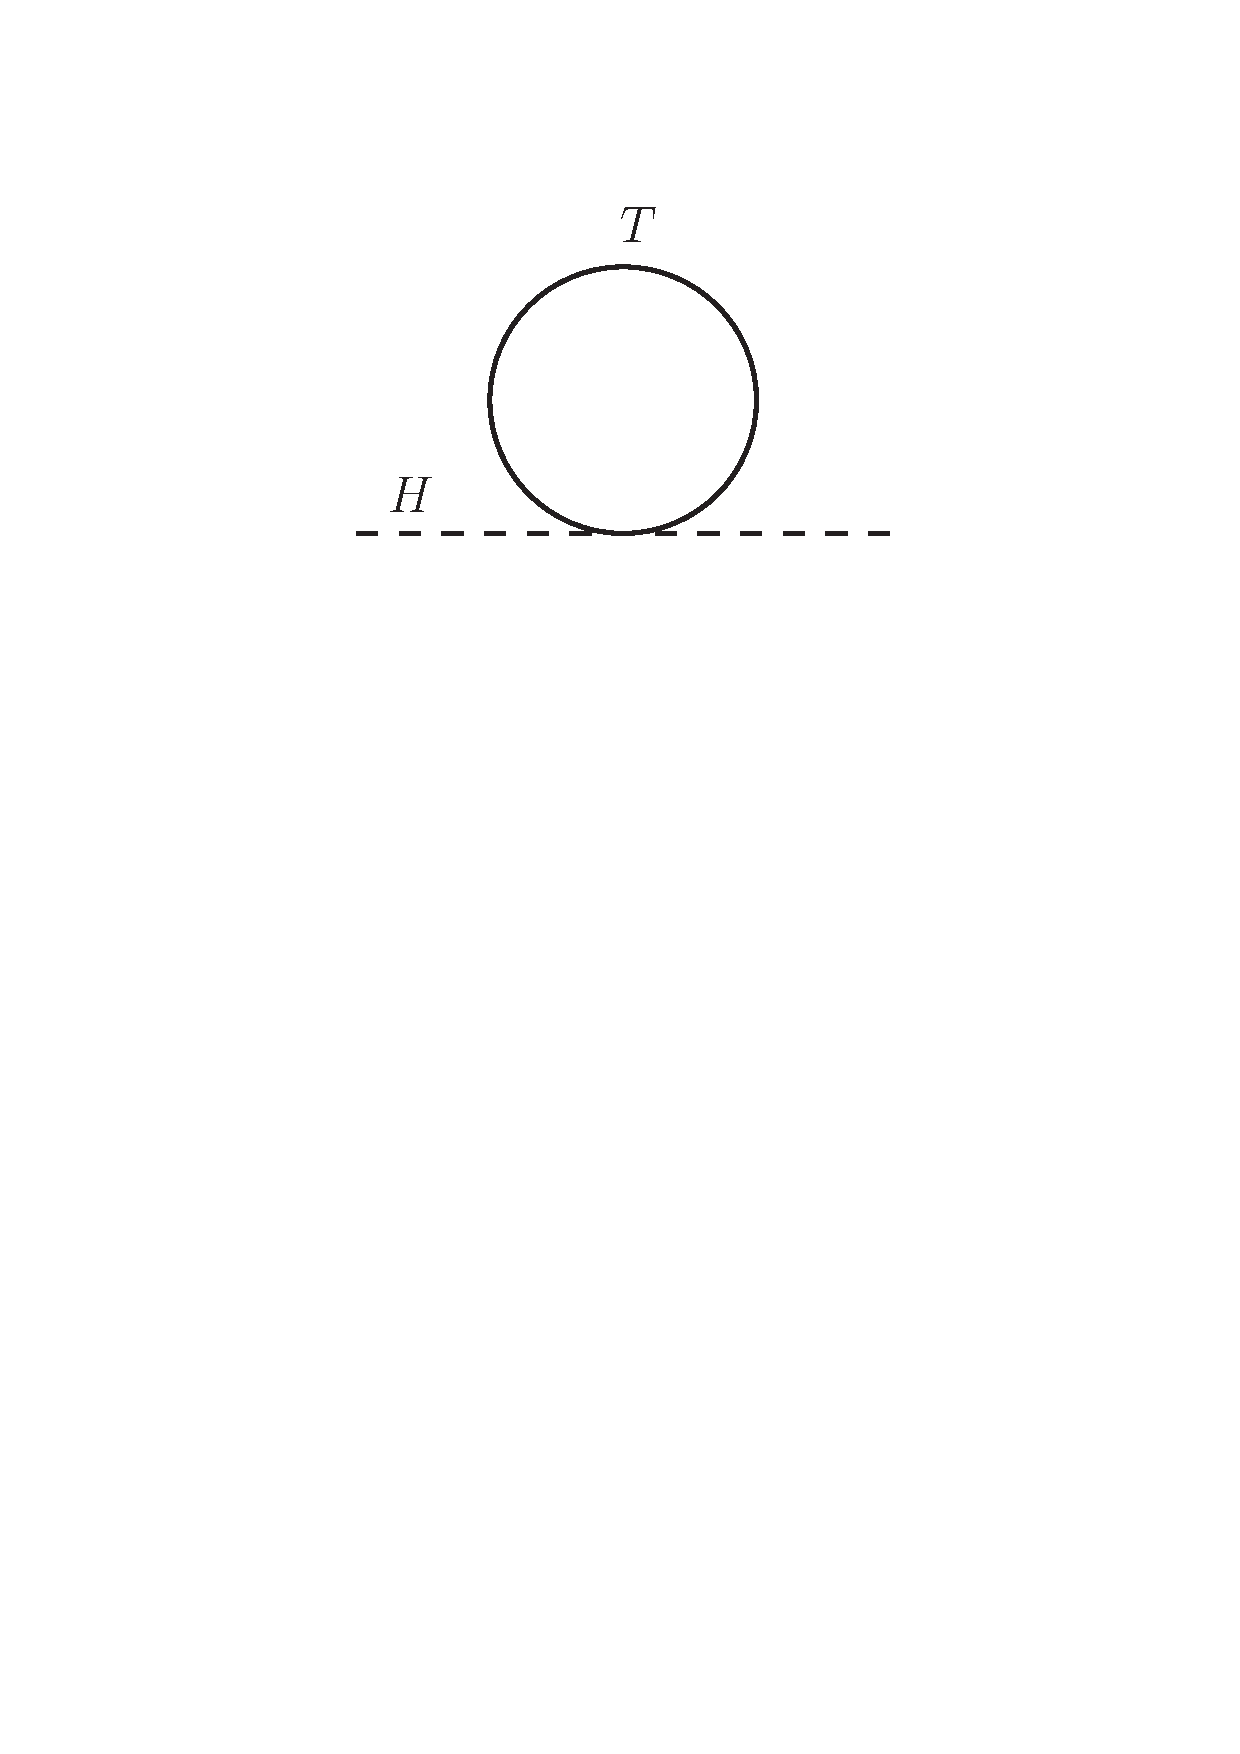
\includegraphics[width=0.92\textwidth]{Theory/FeynmanGraphs/loop_T_good}
    \caption{} \end{subfigure}
	\caption{One-loop contributions to the Higgs boson mass term from (a) the top quark and (b,c) a vector-like top partner.}
          \label{fig:VLQ_loop}
\end{center}
\end{figure}

These new particles can appear as $SU(2)_L$ singlets, doublets or triplets. Their naming and charges is shown in table~\ref{tab:VLQ_tuples}.
\begin{table}[tb]
  \centering
  \begin{minipage}{.4\textwidth}
    \begin{tabular}{cc}
      \toprule
      \toprule
      \textbf{VLQ} & \textbf{Electric charge} \\
      \midrule
      X   & +5/3  \\
      T   & +2/3  \\
      B   & -1/3  \\
      Y   & -4/3  \\
      \bottomrule
      \bottomrule
    \end{tabular}
  \end{minipage}
  \begin{minipage}{.4\textwidth}
    \begin{tabular}{cc}
      \toprule
      \toprule
      \textbf{Multiplet} & \textbf{Hypercharge} \\
      \midrule
      \multicolumn{2}{c}{ Singlets } \\
      $\left(T     \right)$   & $+2/3$  \\
      $\left(B     \right)$   & $-1/3$  \\
      \midrule
      \multicolumn{2}{c}{ Doublets } \\
      $\left(X,T   \right)$   & $+7/6$  \\
      $\left(T,B   \right)$   & $+1/6$  \\
      $\left(B,Y   \right)$   & $-5/6$  \\
      \midrule
      \multicolumn{2}{c}{ Triplets } \\
      $\left(X,T,B \right)$   & $+2/3$  \\
      $\left(T,B,Y \right)$   & $-1/3$  \\
      \bottomrule
      \bottomrule
    \end{tabular}
  \end{minipage}
  \caption{Charge and hypercharge assignment for vector-like quarks in different $SU(2)$ representations.}
  \label{tab:VLQ_tuples}
\end{table}
A mass term for vector-like quarks can be directly inserted into the Lagrangian without breaking the gauge symmetry, so these quarks are also unique in that their coupling to the Higgs field is unrelated to their mass. Therefore there are no constraints on the existence of vector-like quarks arising from the measured Higgs boson production \xsec, since the contribution to loop-induced Higgs boson couplings, $ggH$ and $\gamma\gamma H$, is suppressed by the heavy quark mass.

\subsubsection{Production}
Vector-like quarks can be pair-produced via QCD interactions, or singly produced in association with SM quarks via electroweak interactions. 
The process of pair production through QCD interactions is completely analogous to pair production of SM top quarks, and only depends on \alphas\ and the mass of the heavy quark:
\begin{equation*}
  gg, q\bar{q} \rightarrow Q\bar{Q},\quad \text{with}\ Q = T,B,X,Y .
  \label{VLQ_pairproduction}
\end{equation*}
Single production via electroweak interaction is subdominant for masses below $m_Q \sim 800 - 1000 \gev$, but becomes important for higher masses due to phase-space suppression of pair production. It also depends on the couplings between the new quarks and the $W$ and $Z$ bosons~\cite{Atre:2011ae,Aguilar-Saavedra:2013qpa}:

\begin{equation*}
  qq' \xrightarrow{V^*} qQ,\quad \text{with}\ V = W,Z .
  \label{VLQ_singlepairproduction}
\end{equation*}

\begin{figure}[tb!]
  \centering
  \begin{subfigure}{0.35\textwidth}
    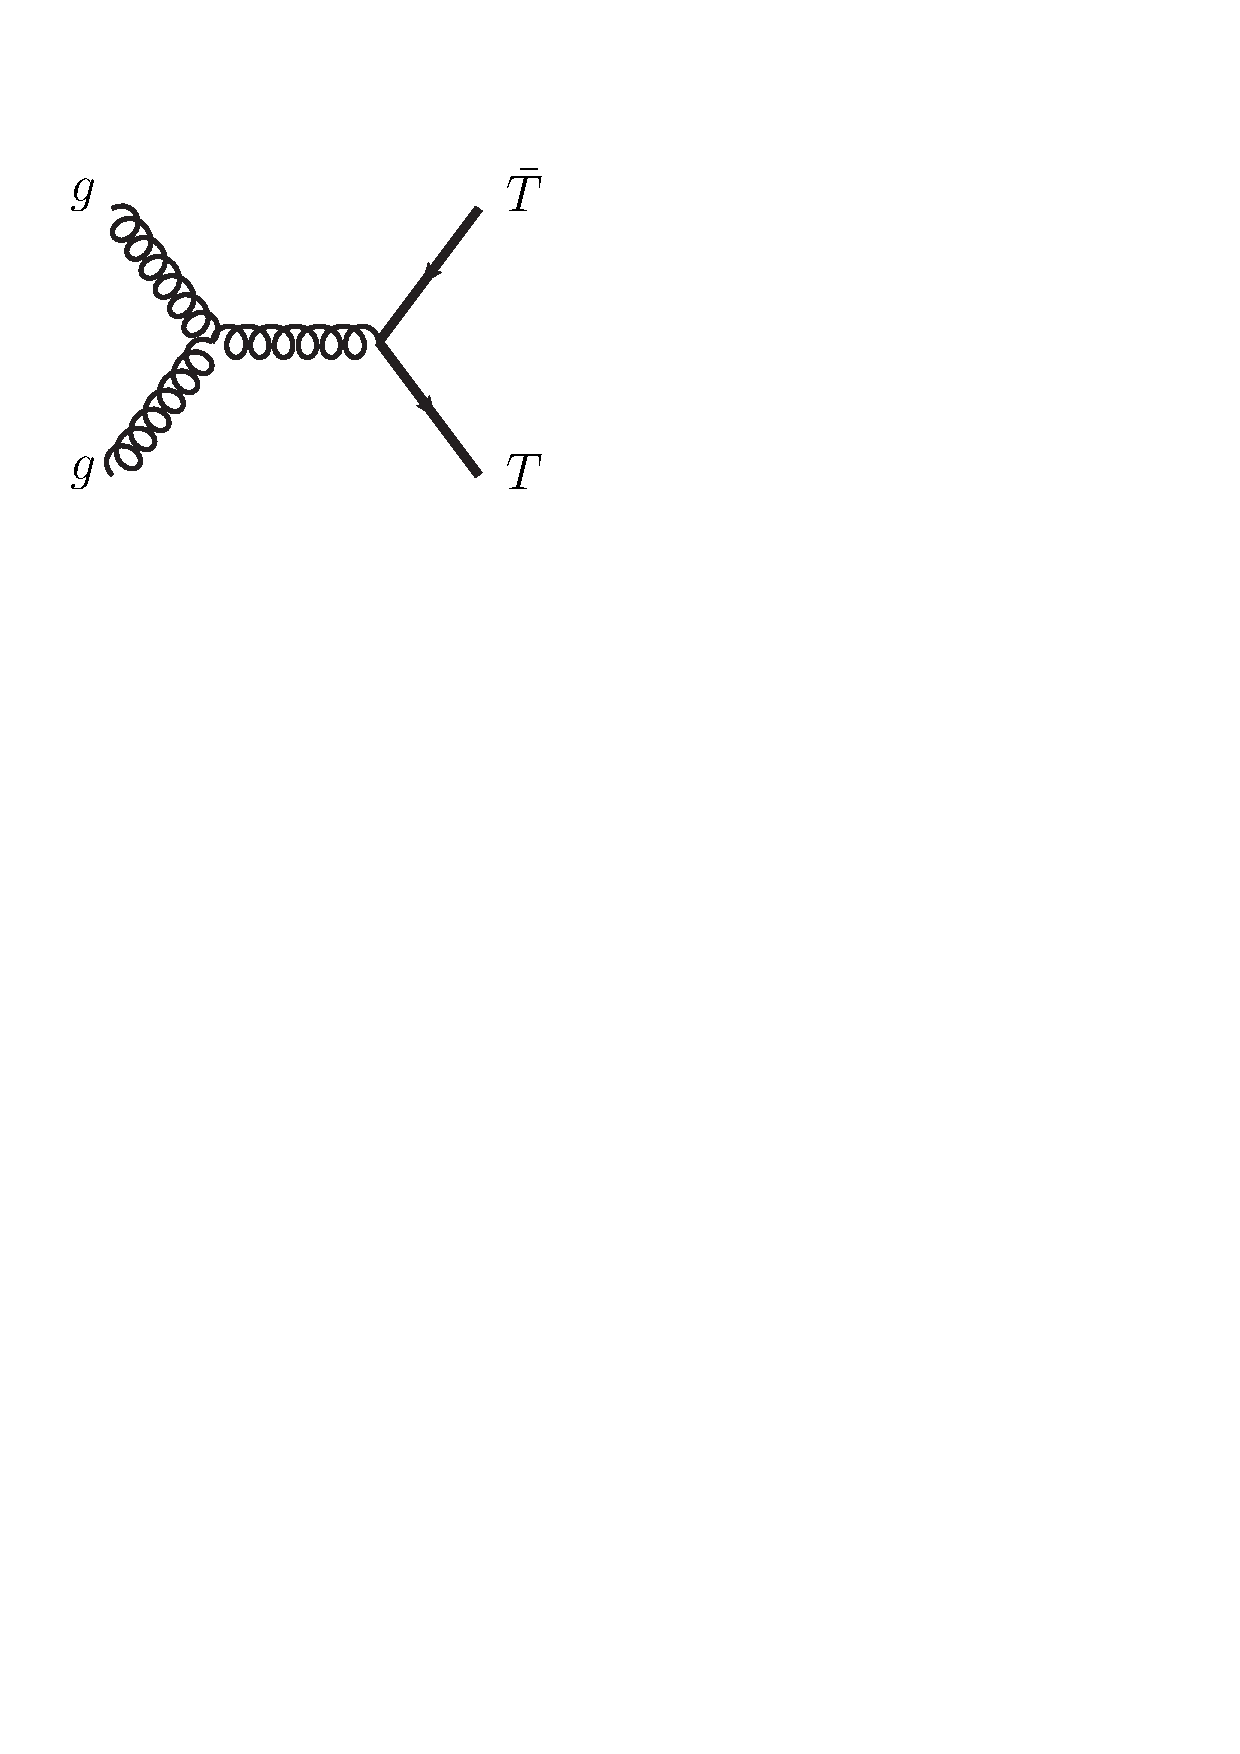
\includegraphics[width=\textwidth]{Theory/FeynmanGraphs/T_pairProd_good.pdf}
  \caption{}
  \label{fig:T_pairProd_good}
\end{subfigure}
  \begin{subfigure}{0.35\textwidth}
    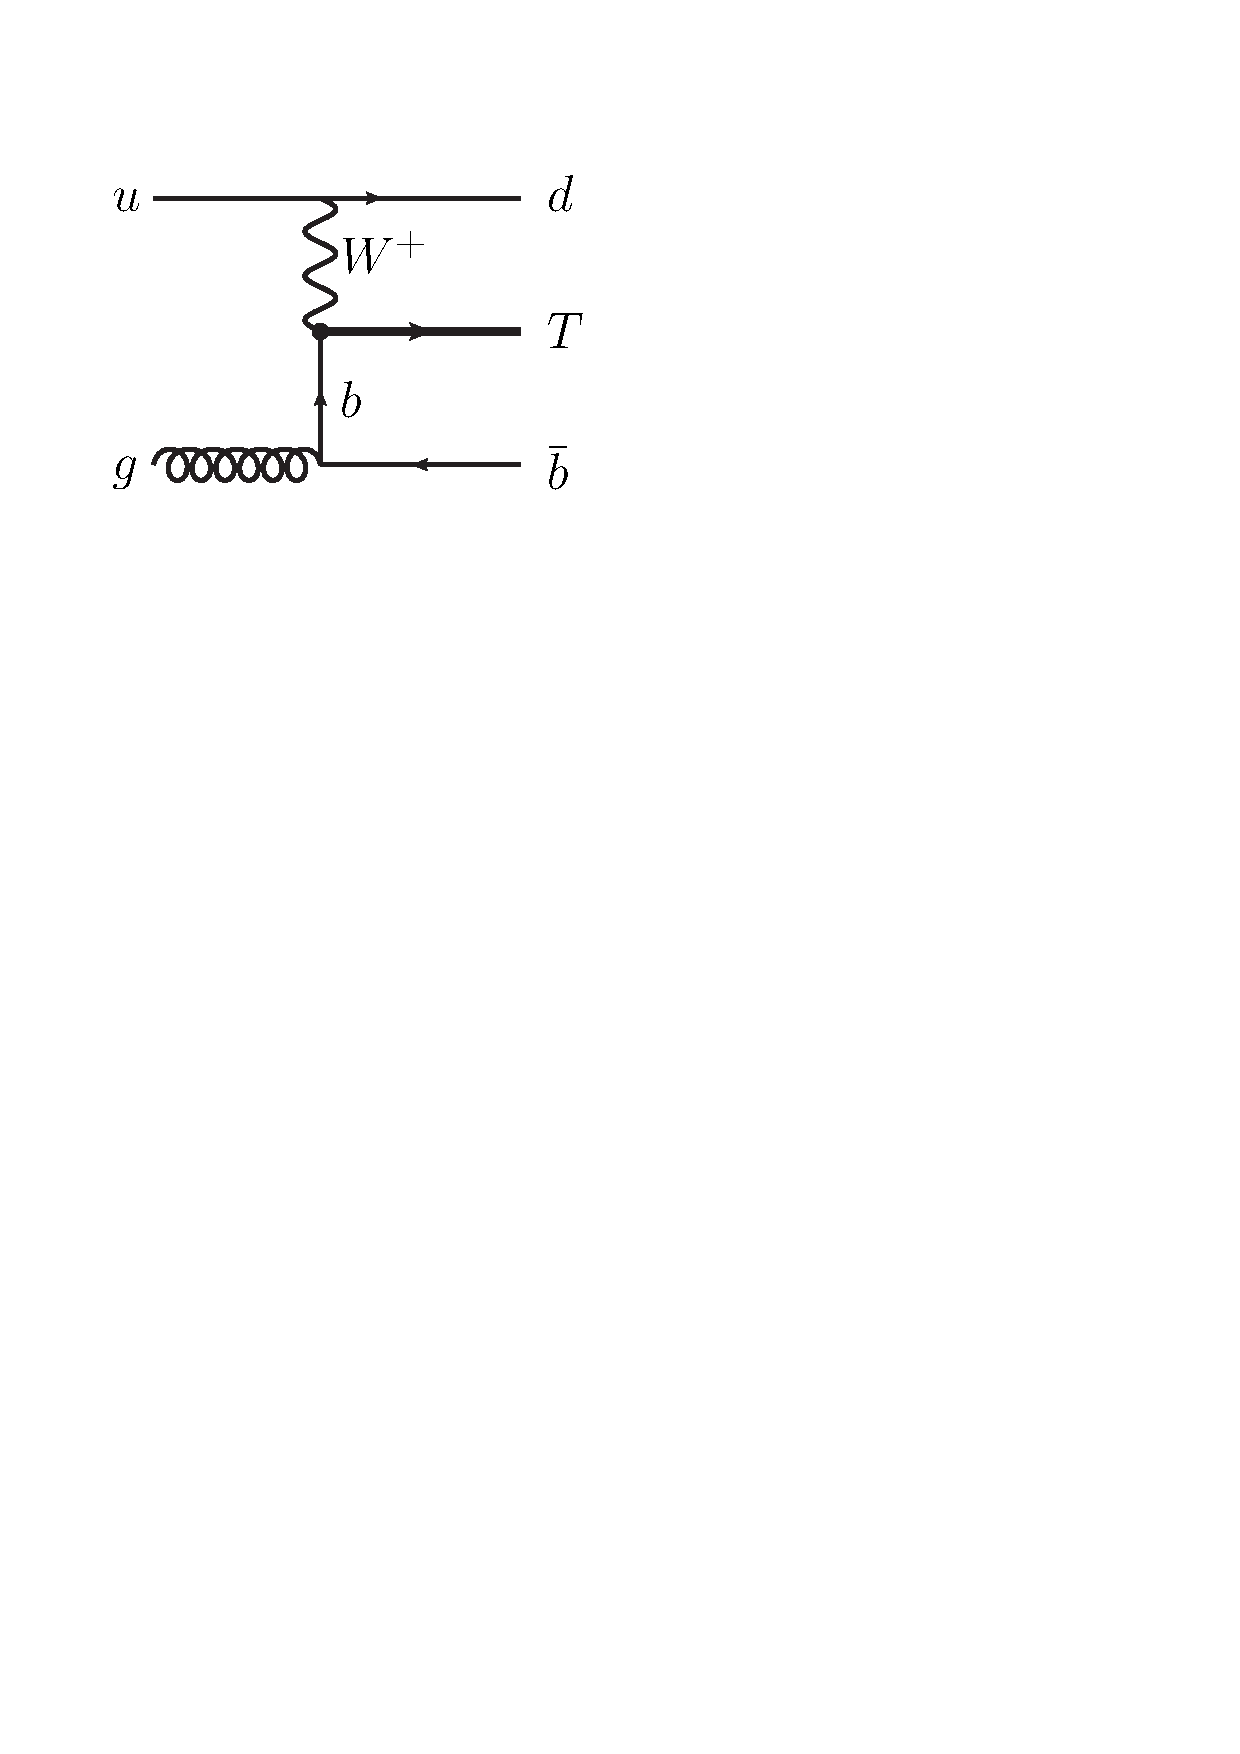
\includegraphics[width=\textwidth]{Theory/FeynmanGraphs/T_singleProd_good.pdf}
  \caption{}
  \label{fig:T_singleProd}
\end{subfigure}
\caption{Example Feynman diagrams for (a) pair production of vector-like top quarks and (b) single production of a vector-like top quark.}
  \label{fig:T_Prod}
\end{figure}

Example Feynman diagrams for pair and single production of vector-like quarks are shown in figure~\ref{fig:T_Prod}.
Figure~\ref{fig:VLQ_production} shows the \xsec\ for pair production and single production in the $t$-channel versus the mass of the vector-like quarks. For a given value of the mass the coupling is set to the maximum allowed by indirect constraints~\cite{Aguilar-Saavedra:2013qpa}.

\begin{figure}[bt!]
  \centering
  \includegraphics[width=0.55\textwidth]{Theory/Figures/VLQ_production.eps}
\caption{Production \xsec\ for heavy quarks  in \pp\ collisions at $\sqrt{s}=\unit[8]{\tev}$ as a function of their mass, for pair production and for single production in different channels.}
  \label{fig:VLQ_production}
\end{figure}

\subsubsection{Decay}
Vector-like quarks decay through electroweak interactions into SM particles. In a general scenario the allowed decays are:

\begin{align*}
  T &\rightarrow W^+b, Zt, Ht \\
  B &\rightarrow W^-t, Zb, Hb \\
  X &\rightarrow W^+t \\
  Y &\rightarrow W^-b~. \\
  \label{VLQ_decays}
\end{align*}

Vector-like quarks can decay via flavor-changing neutral currents since they break the GIM mechanism~\cite{PhysRevD.2.1285}. 
In order to be consistent with precision electroweak data, a small mass splitting between vector-like quarks belonging to the same $SU(2)$ multiplet is required~\cite{Aguilar-Saavedra:2013qpa}, which forbids cascade decays such as $T \to WB$, and leaves direct decays into SM particles as the only possibility. 
In general, the new quarks are expected to couple mainly to the third generation since the mixing of the vector-like quarks with SM quarks is of order $m/M$, where $m$ and $M$ are the masses of the SM quarks and the new quarks respectively~\cite{delAguila:1982fs}.
Couplings to lighter generations, although not favored, are not excluded and can lead to flavor-changing neutral top interactions~\cite{delAguila:1998tp}.

 For the isospin singlets \T\ and \B\ all three decays are possible. However, the scenario is different for the isospin doublets. In the case of a $\left(T, B\right)$ doublet, the two quarks are almost degenerate in mass and the decays strongly depend on the mixing factors of the extended CKM matrix $V_{Tb}$ and $V_{tB}$. If $V_{Tb} \sim V_{tB}$ then the \T\ and \B\ quarks have the same decays as the corresponding singlets but different angular distributions since only the right-handed component of $\left(T, B\right)$ couples to the SM quarks. 
 In the most natural case where $V_{Tb} \muchless V_{tB}$, then the mixing of the heavy quarks with the SM top quark is much stronger, and the $\T \rightarrow Wb$ decay is suppressed, as well as $\B \rightarrow Hb$ and $\B \rightarrow Zb$. This scenario, $V_{Tb} \muchless V_{tB}$, will be assumed throughout this dissertation. Table~\ref{tab:VLQ_decay} summarizes the possible decays of vector-like quarks.

 \begin{table}[b!]
   \centering
   \begin{tabular}{ccc}
   \begin{tabular}{cc}
     \toprule
     \toprule
     Singlets & Decay modes \\
     \midrule
     & \\
     $X$ & $W^+t$ \\
     & \\
     $T$ & $W^+b,\, Ht,\, Zt$ \\
     & \\
     $B$ & $ W^-t,\, Hb,\, Zb$ \\
     & \\
     $Y$ & $W^-b$ \\
     & \\
     & \\%one empty line
     \bottomrule
     \bottomrule
   \end{tabular}

   & 

   \begin{tabular}{cc}
     \toprule
     \toprule
      Doublets & Decay modes\\
     \midrule
     &\\%one empty line
     \multirow{2}{*}{$\left(\begin{array}{c}X \\ T\end{array}\right)$} & $W^+t$\\
     & $Ht,\, Zt$\\
     &\\
     \multirow{2}{*}{$\left(\begin{array}{c}T \\ B\end{array}\right)$} & $ Ht,\, Zt$ \\%$W^+b,\, Ht,\, Zt$\\
     & $ W^-t$\\%$ W^-t,\, Hb,\, Zb$\\
     & \\
     \multirow{2}{*}{$\left(\begin{array}{c}B \\ Y\end{array}\right)$} & $Hb,\, Zb$\\
     & $W^-b$\\
     &\\%one empty line
     \bottomrule
     \bottomrule
   \end{tabular}
   & 

   \begin{tabular}{cc}
     \toprule
     \toprule
      Triplets & Decay modes\\
     \midrule
     &\\%one empty line
     \multirow{3}{*}{$\left(\begin{array}{c}X \\ T \\ B\end{array}\right)$} & $ W^+t$ \\
     & $W^+b,\, Ht,\ Zt$\\
     & $Hb,\, Zb$\\
     &\\%one empty line
     \multirow{3}{*}{$\left(\begin{array}{c}T \\ B \\ Y\end{array}\right)$} & $Ht,\, Zt$\\
     & $W^-t,\, Hb,\, Zb$\\
     & $W^-b$\\
     &\\%one empty line
     &\\%one empty line
     \bottomrule
     \bottomrule
   \end{tabular}
   \end{tabular}
   \caption{Allowed decay modes for vector-like singlets, doublets and triplets.}
     \label{tab:VLQ_decay}
   \end{table}

 The branching ratios of the vector-like quarks depend on the model but also on the heavy quark mass.
 Figure~\ref{fig:VLQ_BR} shows the decay branching ratios of the vector-like top and bottom partners for isosinglets and isodoublets as a function of the heavy-quark mass.

 \begin{figure}
   \centering
   \begin{subfigure}{0.49\textwidth}
     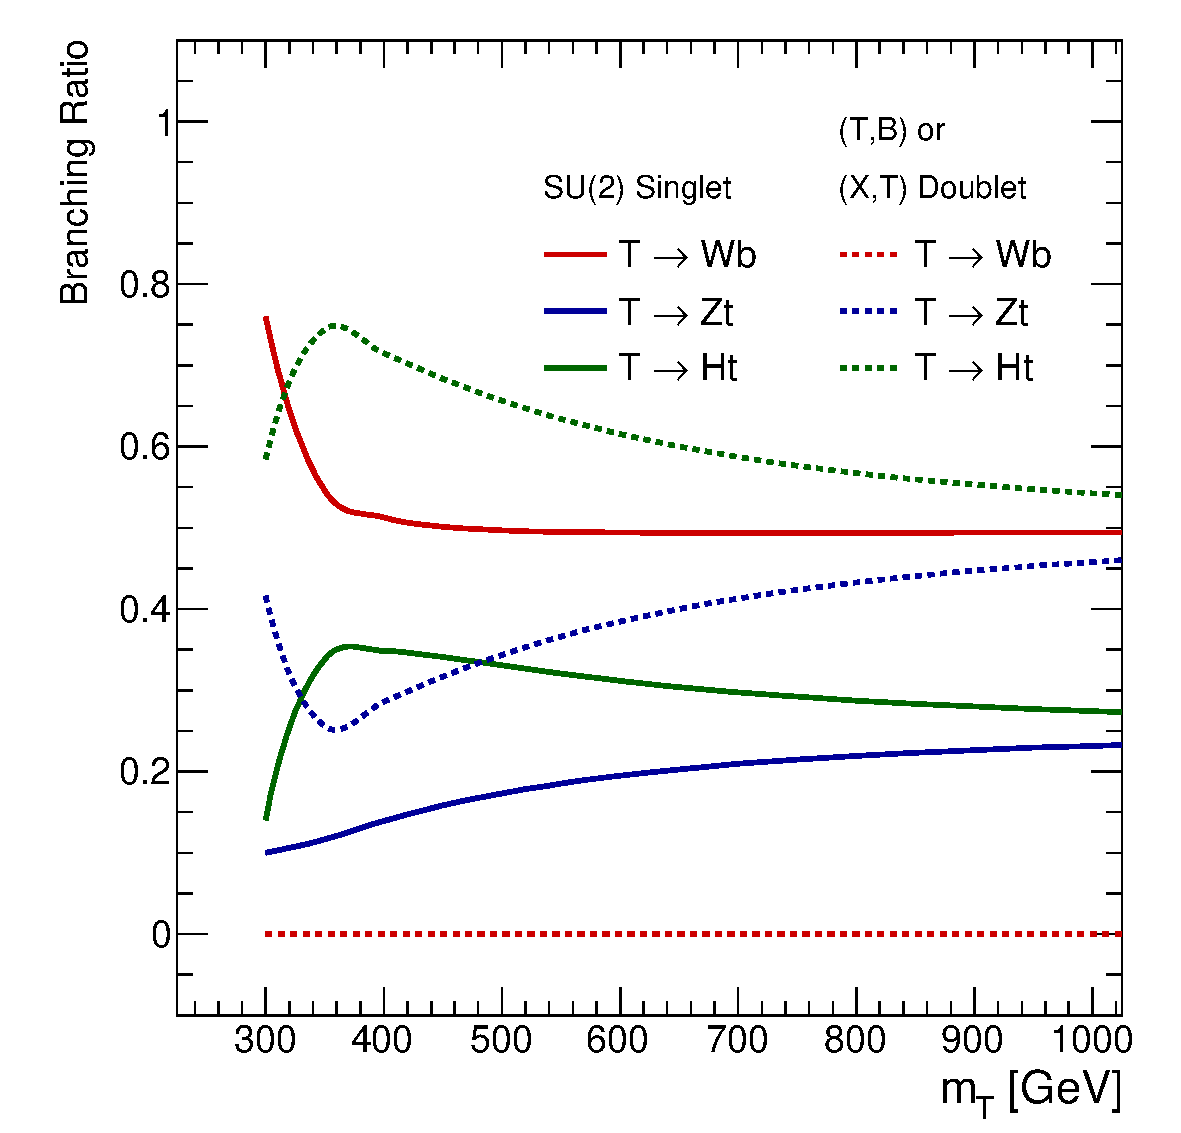
\includegraphics[width=\textwidth]{Theory/Figures/fig_02a.pdf}
     \label{fig:vltbrs}
     \caption{}
 \end{subfigure}
   \begin{subfigure}{0.49\textwidth}
     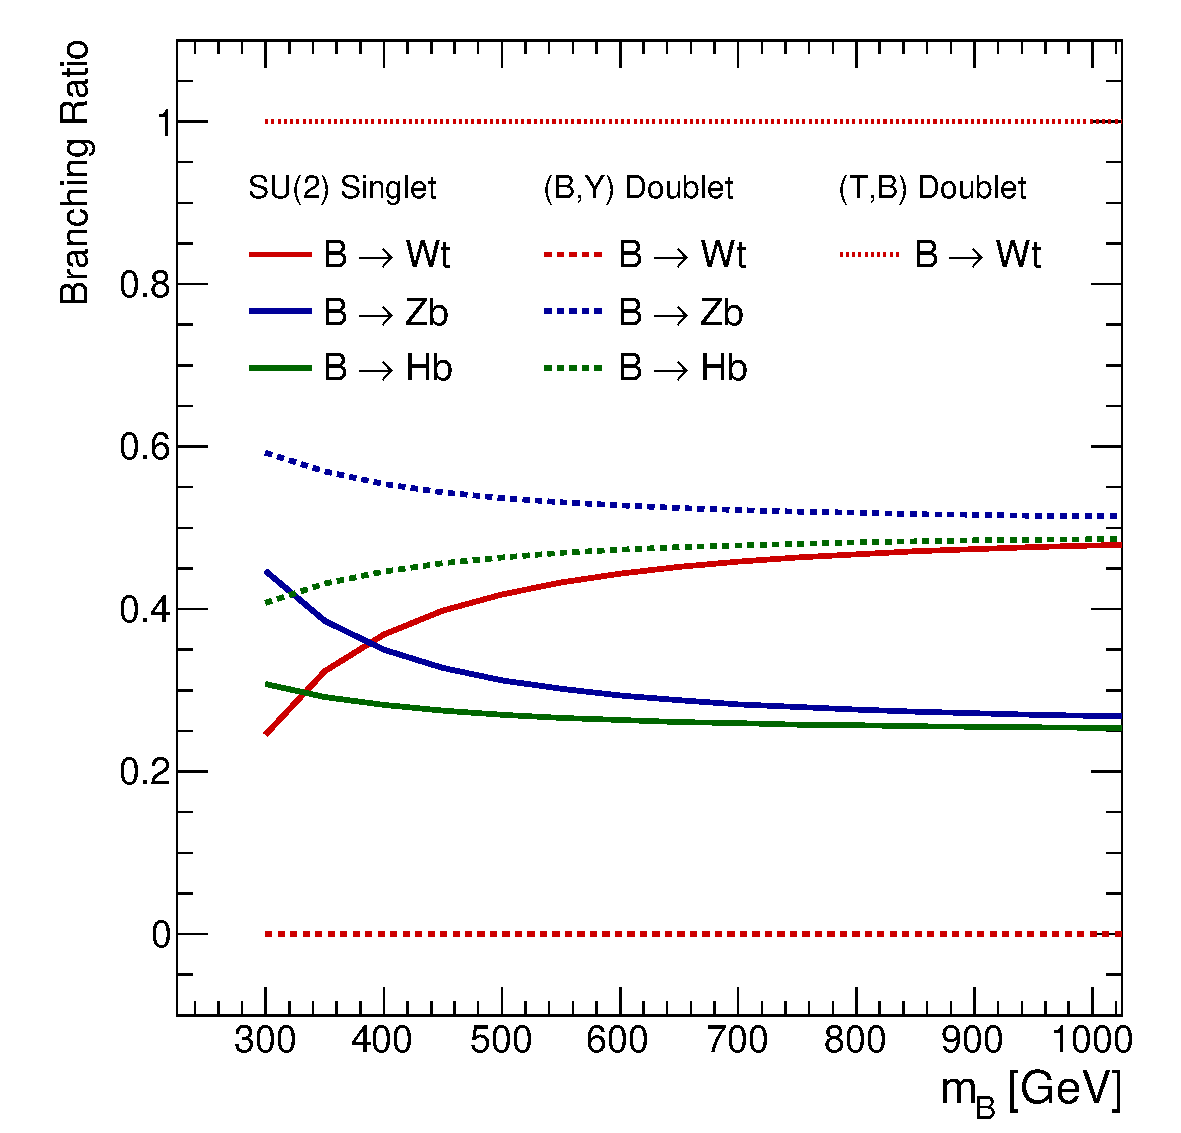
\includegraphics[width=\textwidth]{Theory/Figures/fig_02b.pdf}
     \label{fig:vlbbrs}
     \caption{}
 \end{subfigure}
     \caption{Branching ratio of vector-like top (a) and bottom (b) partners as a function of the heavy quark mass $m_T$ and $m_B$ respectively for isosinglets and isodoublets.}
   \label{fig:VLQ_BR}
 \end{figure}

 After pair production, the decay of at least one vector-like top into a Higgs boson and a top quark produces, following the dominant $H\to b\bar{b}$ decay, a \ttbar-like final state with additional heavy-flavor jets, which is the final state targeted in this dissertation.

\subsection{Bosonic top partners: stops}
The inclusion of bosonic partners of the top quark ($\tilde{t}$, stops) prevents the unnatural fine-tuning
of the Higgs mass, provided that the stops have masses not too far above the weak scale and typically below \unit[1]{\tev}.

Searches for $\st_1$ pair production are challenging because the \xsec\ is 
significantly smaller than for $t\bar{t}$ production (about a factor of six lower for 
$m_{\st_1}\sim m_t$) and the \xsec\ decreases rapidly with increasing $m_{\st_1}$. Direct
searches for $\st_1$ pair production are particularly sensitive in the regime where
$m_{\st_1}\gg m_t + m_{\neut}$, giving rise to signatures with large $\met$ that allow to
distinguish the signal from the $t\bar{t}$ background. 
However, those searches have very limited sensitivity in the kinematic region where $m_{\st_1}\sim m_t + m_{\neut}$, 
given the very similar kinematic features between signal and background. In this scenario,
other strategies need to be pursued to identify topologies with increased separation between
signal and background. One possibility is to search for pair production of
the heavier stop quark, $\st_2$, with subsequent decay $\st_2 \to Z\st_1$, $H\st_1$ and
$t \neut$. This decay chain results in final states with associated production of $t\bar{t}$ with one or more boson ($Z$ or $H$)\footnote{
 For consistency with the other analyses, the capital letter $H$ is used to denote the light Higgs boson. 
 In supersymmetric models the capital letter is commonly used to denote the heavier Higgs boson, while the lowercase $h$ is used to refer to the lighter mass eigenstate which is identified with the \unit[125]{\gev} state discovered at the LHC. Throughout the text, the \unit[125]{\gev} Higgs boson will be denoted by the capital letter $H$ regardless of the model being studied.
},
which provide additional handles to suppress the background. 
In particular the decay through a Higgs boson, and the subsequent $H \to \bbbar$ decay results in a \ttbar\ final state with additional heavy-flavor jets. %Some contribution from decays through a $Z$ boson with $Z \to \bbbar$ is also expected.

For the analysis described in this dissertation, a simplified SUSY model is considered where only the top quark partners and the lightest neutralino, \stopone, \stoptwo, \neutralino, are considered to be kinematically accessible at the LHC. The masses for the rest of the SUSY spectrum are set arbitrarily high. Therefore, production and decay processes involving other SUSY particles such as $\gluino \to \stopone t$ or $\stopone \to \chinoonepm b$ are not considered.

\subsubsection{Production}

\begin{figure}[!tb]
\begin{center}
\mbox{
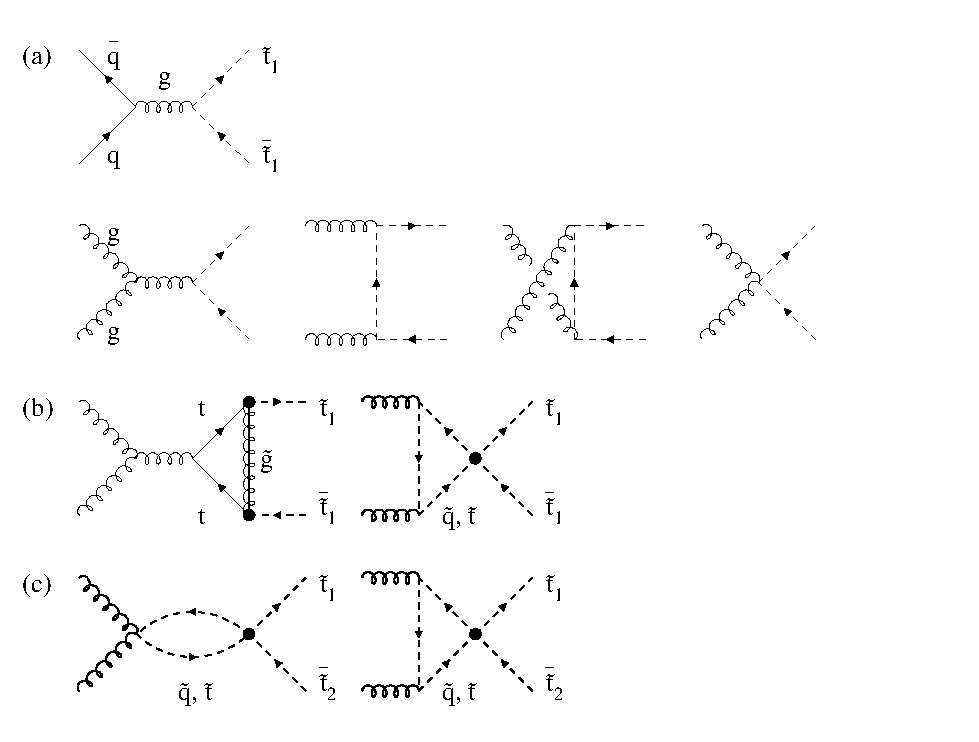
\includegraphics[trim=0.8cm 5.7cm 0cm 0cm, clip=true, width=0.995\textwidth]{Theory/Figures/feyn_fin.eps}
}
\end{center}
\caption{Born diagrams for quark-antiquark annihilation and gluon fusion, leading to pairs of stop pair production.}
\label{fig:StopProductionDiagrams}
\end{figure}

At hadron colliders, stop pairs can be produced at leading order in quark-antiquark annihilation and gluon-gluon fusion:

\begin{equation}
\begin{matrix}
q \bar{q} \rightarrow & \stopone \antistopone, & \stoptwo \antistoptwo~,\\
gg        \rightarrow & \stopone \antistopone, & \stoptwo \antistoptwo~,\\
\end{matrix}
\label{eq:DirectStopSbottomProduction}
\end{equation}
and the relevant leading order diagrams for these processes are found in figure~\ref{fig:StopProductionDiagrams}.
The production of \stopone\ and \stoptwo\ pairs is completely identical and depends only on $\alphas$ and the mass of the particle. Although the analysis presented in this dissertation targets the pair production of \stoptwo, the process of \stopone\ pair production is also present in the simplified model and has to be taken into account. 
The production of mixed \stopone \antistoptwo\ or \stoptwo \antistopone\ pairs is suppressed as the \xsec\ is of order $\alphas^4$ and will not be considered~\cite{Beenakker:1997ut}.

\subsubsection{Decay}
The possible decays of the stop particles are limited within the simplified SUSY model:
\begin{align*}
  \stopone &\to t \neutralino \\
  \stoptwo &\to t \neutralino, ~\stopone H, ~\stopone Z, 
  \label{eq:stop_decay}
\end{align*}
and the \neutralino\ is considered the LSP and is therefore stable.

The branching fractions to the three possible decays of the \stoptwo\ are not predicted by the model and will be considered free parameters. In the parameter region where $m_{\stoptwo} < m_{\stopone} + m_H$, the decay through a Higgs boson is suppressed. If $m_{\stoptwo} < m_{\stopone} + m_Z$, only the decay to a top quark and neutralino is possible. Figure~\ref{fig:stop_decay} shows two examples of \stoptwo\ decays to the different allowed particles.

\begin{figure}[tb!]
  \centering
  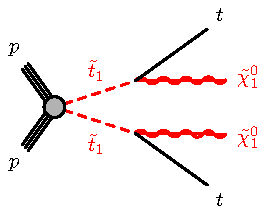
\includegraphics[width=0.32\textwidth]{Theory/FeynmanGraphs/FeynmanGraphsSUSY/stst-ttN1N1.eps}
  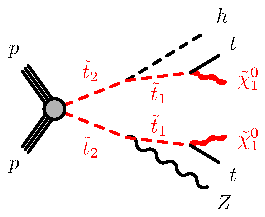
\includegraphics[width=0.32\textwidth]{Theory/FeynmanGraphs/FeynmanGraphsSUSY/st2st2-ZhttN1N1.eps}
  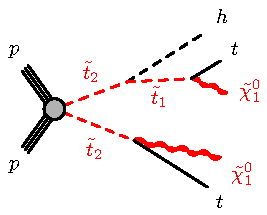
\includegraphics[width=0.32\textwidth]{Theory/FeynmanGraphs/FeynmanGraphsSUSY/st2st2-httN1N1.eps}
  \caption{Examples of decays of \stopone\ and \stoptwo\ particles in the different allowed decay channels.}
  \label{fig:stop_decay}
\end{figure}

\subsection{Four-top-quark production}
The production rate of four-top-quark events is very small in the SM, with a \xsec\ of $\sigma_\fourtop \approx \unit[1]{fb}$ at $\sqrt{s}=\unit[8]{\tev}$~\cite{Barger:1991vn,Barger:2010uw}. However many BSM theories predict an increase of this final state, usually through the pair production of a new particle decaying to a top-antitop pair. The subsequent decay produces a spectacular final state which, in the case of one leptonic $W$ decay, produces up to ten jets with four of them originating from $b$-quarks.
Figure~\ref{fig:fourtop_FD} depicts representative LO Feynman diagrams for four-top-quark production within the SM and the BSM scenarios considered in this dissertation. 

The phenomenology of the different models predicting an increase of the four-top-quarks final state is discussed in the following.

\begin{figure}[tbp]
\centering
\begin{subfigure}{0.49\textwidth} 
\centering
  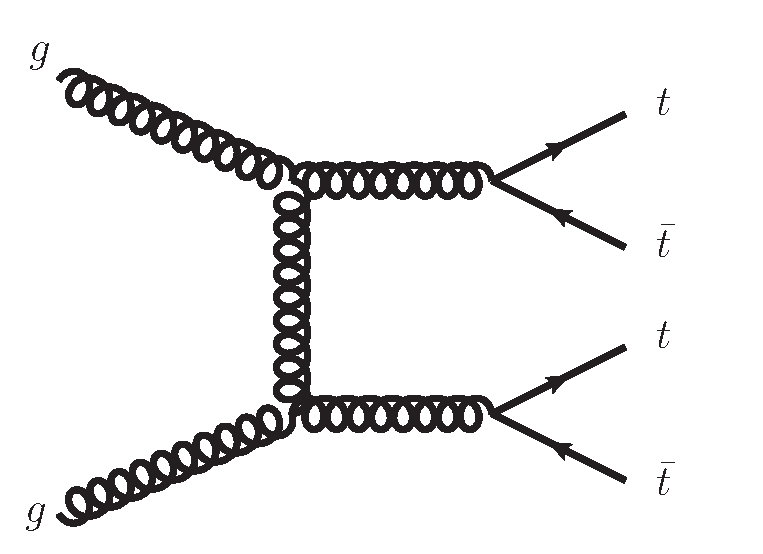
\includegraphics[width=0.66\textwidth]{Theory/FeynmanGraphs/4tops_SM.eps}
  \caption{}\label{fig:fourtop_SM} \end{subfigure}
\begin{subfigure}{0.49\textwidth} 
\centering
  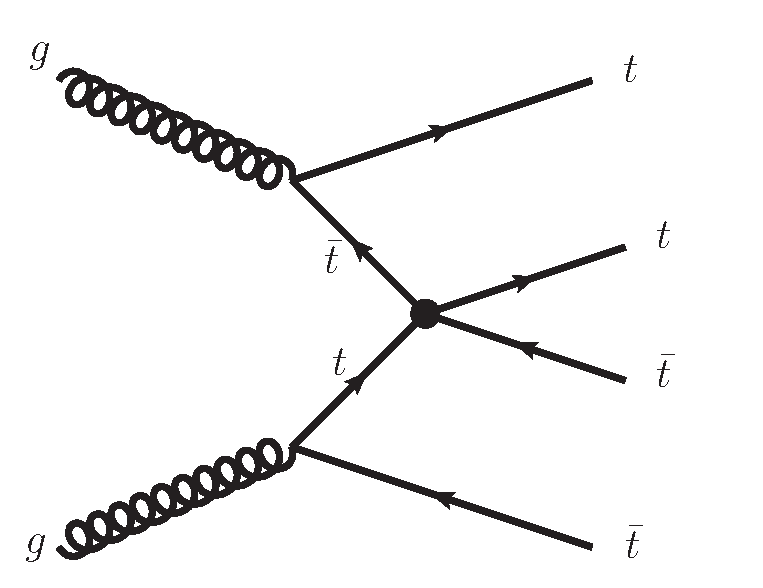
\includegraphics[width=0.60\textwidth]{Theory/FeynmanGraphs/4tops_CI.eps}
  \caption{}\label{fig:fourtop_CI} \end{subfigure}
\\
\begin{subfigure}{0.49\textwidth} 
\centering
  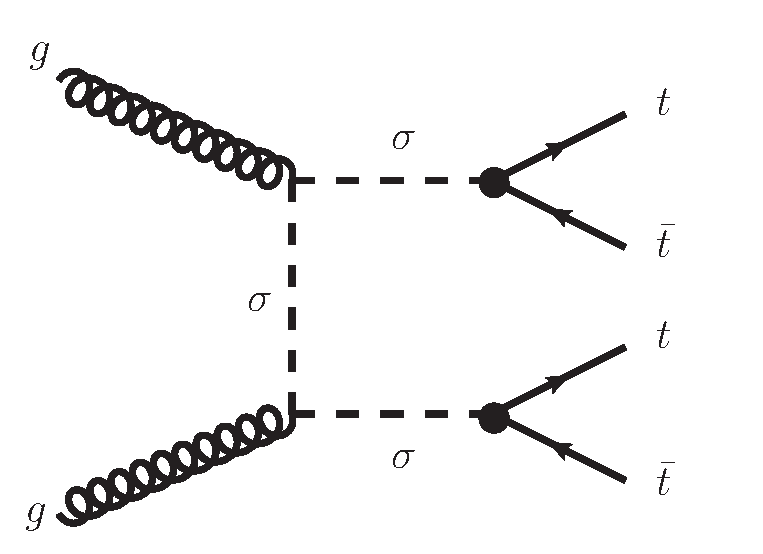
\includegraphics[width=0.66\textwidth]{Theory/FeynmanGraphs/4tops_sgluon.eps}
  \caption{}\label{fig:fourtop_sgluon} \end{subfigure}
\begin{subfigure}{0.49\textwidth} 
\centering
  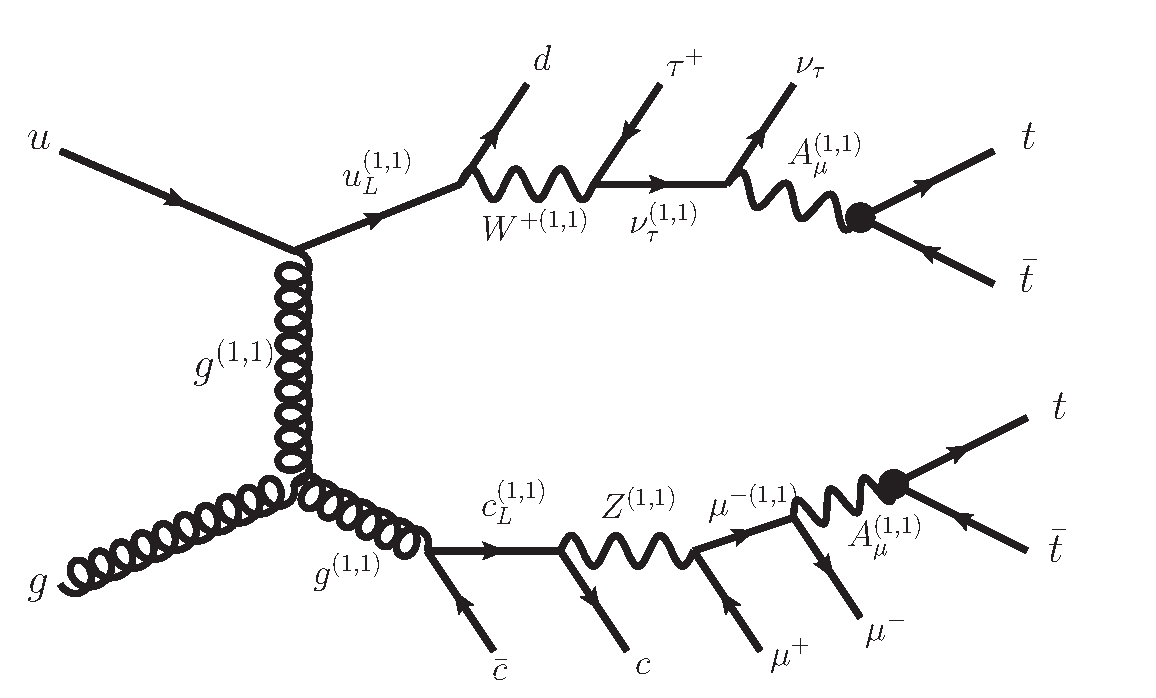
\includegraphics[width=0.80\textwidth]{Theory/FeynmanGraphs/4tops_UEDRPP.eps}
  \caption{}\label{fig:fourtop_UEDRPP} \end{subfigure}
\caption{Representative leading-order Feynman diagrams for four-top-quark production within (a) the SM 
and several BSM scenarios: (b) via an effective four-top-quark interaction in an effective field theory 
model, (c) via scalar-gluon-pair production, and (d) via cascade decays from Kaluza-Klein excitations in an universal extra dimensions 
model with two extra dimensions compactified under the real projective plane. }
\label{fig:fourtop_FD}
\end{figure}

\subsubsection{Kaluza-Klein modes}
\label{subsubsec:KKmodes}
In the model with two universal extra dimensions discussed in section~\ref{subsubsec:UED}, gauge bosons propagating in the extra dimensions produce a tower of KK vector modes. The compactification of the two extra dimensions under the real projective plane geometry (2UED/RPP) leads to the discretization of the momenta along these directions. The set of solutions of the field equation are described by two integers $(j,k)$, referred to as KK numbers. A \textit{tier} $(j,k)$ is the set of particles with same KK numbers. At leading-order the masses of the particles within a tier $(j,k)$ are: 
\begin{equation}
  m^2 = \frac{j^2}{R^2_4}+\frac{k^2}{R^2_5}~, 
  \label{eq:tier_masses}
\end{equation}
where $\pi R_4$ and $\pi R_5$ are the size of the two extra dimensions.
The model is parameterized by $R_4$ and $R_5$ or, alternatively, by 
$m_{\KK}=1/R_4$ and $\xi=R_4/R_5$. 
Particles from the level-1 modes ($j+k=1$)  would decay into soft leptons and jets plus missing energy~\cite{Cheng:2002ab}, making their discovery challenging. However, level-2 modes can be produced at colliders, their decay into level-1 modes is kinematically forbidden and have large branching fractions for decays into a pair of SM particles. 

Four-top-quark production can arise from tier $(1,1)$, where particles
from this tier have to be pair produced because of symmetries of the model. Then they chain-decay to the 
lightest particle of this tier, the heavy photon $A^{(1,1)}$, by emitting SM particles (see figure~\ref{fig:fourtop_UEDRPP}). 
The branching ratios of $A^{(1,1)}$ into SM particles are not predicted by the model, although the decay 
into $\ttbar$ is expected to be dominant~\cite{Cacciapaglia:2011kz}. Four-top-quark events can also arise from 
tiers $(2,0)$ and $(0,2)$ via a similar mechanism. In this case the expected \xsec\ for four-top-quark production 
is reduced compared to that from tier $(1,1)$ since each state in tiers $(2,0)$ and $(0,2)$ can decay 
directly into a pair of SM particles or into a pair of states in tiers $(1,0)$ or $(0,1)$ via bulk interactions, 
resulting into smaller branching ratios for decay into $t\bar{t}$~\cite{Cacciapaglia:2011kz}.
In the following, when considering four-top-quark production from a given tier, it will be
assumed that the $A$ photon in that tier decays with 100\% branching ratio into $\ttbar$ 
while $A$ photons from other tiers cannot decay into $\ttbar$.

Due to the geometry of the space an $SO(2)$ symmetry arises, usually referred to as KK parity. This symmetry forbids the decay of the lightest particle from tier $(1,0)$ (and tier $(0,1)$ in case of equal radii) to SM particles, thus allowing for a natural dark matter candidate~\cite{Cheng:2002ej,Servant:2002aq}. 
Observations of dark matter relic abundance favor values of $m_{\KK}$ between $600\gev$ and $1200\gev$~\cite{Arbey:2012ke}.

\subsubsection{Sgluons}
Scalar particles, which are color-octets, are predicted in several models and are usually referred to as \textit{sgluons}. Some supersymmetric models consider Dirac gauginos~\cite{Plehn:2008ae,Choi:2008ub}, which have a corresponding scalar in the adjoint representation of QCD, and SM-like R-parity.
Sgluon particles are also predicted in non-supersymmetric models~\cite{Kilic:2009mi,Kilic:2008pm,Burdman:2006gy,Calvet:2012rk} such as extra-dimension models and models with a new strong sector leading to scalar pseudo-Goldstone bosons which can be identified with the sgluons.

Once produced through standard strong interactions, a sgluon can decay either to a quark pair or to a gluon pair.
For sgluon masses above twice the top-quark mass, the dominant decay mode is into \ttbar, giving rise to a four-top-quark final state (figure~\ref{fig:fourtop_sgluon}). 
For the analysis described in this dissertation a \unit[100]{\%} branching ratio to top quarks is considered.

\subsubsection{Contact interactions}
The four-top-quarks signatures described in previous sections assume the pair-production of a new particle that can be produced at the LHC.
However when the mass of the new particle is beyond the energy reach of the LHC, its effect on different observables can still be noticeable. An effective field theory (EFT) formalism can be used, where the effect of new physics is described by non-renormalizable operators of higher order~\cite{Degrande:2010kt}. An operator for four-top-quarks contact interaction (see figure~\ref{fig:fourtop_CI}) can be considered:
\begin{equation}
  \lagrangian_{4t} = \frac{C_{4t}}{\Lambda^2}(\bar{t}_R \gamma^\mu t_R)(\bar{t}_R \gamma_\mu t_R)~.
  \label{eq:contact_interaction}
\end{equation}
Only the contact interaction operator with right-handed top quarks is considered as left-handed top quark operators are already strongly constrained by electroweak precision data~\cite{Georgi:1994ha}.

This approach can be used to parameterize composite top quark scenarios~\cite{Pomarol:2008bh,Kumar:2009vs,Lillie:2007hd}, with a new strongly interacting sector or new heavy vector particles predicted in Randall-Sundrum theories~\cite{Guchait:2007jd}.

  \cleardoublepage
  \chapter{The ATLAS experiment at the Large Hadron Collider}
\label{chapter:ATLASDetector}

The Large Hadron Collider (LHC) is the world's highest-energy particle accelerator, designed to collide protons at a \com\ energy of \unit[14]{\tev}.
The ATLAS experiment is one of the two multi-purpose experiments that take advantage of the collisions provided by the LHC.
It has been conceived to pursuit an ambitious physics program, where the first milestone was the discovery of the Higgs boson, achieved in 2012~\cite{Aad:2012tfa,Chatrchyan:2012ufa}.
This chapter introduces CERN's accelerator complex and describes the main aspects of the ATLAS detector at the LHC.


\section{The Large Hadron Collider}
\label{sec:LHC}

The Large Hadron Collider (LHC)~\cite{Evans:2008zzb} is a circular particle accelerator installed in a \unit[27]{km} long underground tunnel, and designed to collide protons at a \com\ energy of $\sqrt{s} = \unit[14]{\TeV}$.
On the accelerator ring four detectors (ALICE~\cite{Aamodt:2008zz}, ATLAS~\cite{Aad:2008zzm}, CMS~\cite{Chatrchyan:2008aa} and LHCb~\cite{Alves:2008zz}) have been built around four different interaction points, to record and study the collisions delivered by the LHC.
ATLAS and CMS are multipurpose experiments designed to study a broad range of physics processes. The LHCb experiment is specialized in the detection of $b$-hadrons, while the ALICE collaboration focuses on the study of heavy-ion collisions.
%The LHC has been designed to collide protons at a \com\ energy of $\sqrt{s} = \unit[14]{\TeV}$.

Since 2010, the LHC has delivered proton-proton ($\pp$) collisions at a \com\ energies of \unit[7]{\TeV} and \unit[8]{\TeV} (in 2011 and 2012, respectively), about half of its nominal energy.
The LHC has produced also lead-ion (Pb-Pb) collisions with a per-nucleon \com\ energy of $\sqrt{s_{NN}} = \unit[2.76]{\TeV}$ and proton-lead (p-Pb) collisions with $\sqrt{s_{NN}} = \unit[5.02]{\TeV}$.

The protons are accelerated to the desired energy through various steps.
First, protons are extracted from the ionization of hydrogen gas and injected in the linear accelerator LINAC2, where they are accelerated to an energy of \unit[50]{\mev}.
They are then transferred into the Proton Synchrotron Booster (PSB) and accelerated up to an energy of \unit[1.4]{\gev}.
A second circular accelerator, the Proton Synchrotron (PS) brings the energy of the protons to \unit[25]{\gev} before injecting them into the Super Proton Synchrotron (SPS).
After being accelerated to \unit[450]{\gev}, the protons finally enter the two LHC beam pipes where they are boosted to energies of up to \unit[4]{\tev}.
A schematic view of the acceleration chain is shown in figure~\ref{fig:accelerator_schema}.

\begin{figure}[!tb]
  \centering
  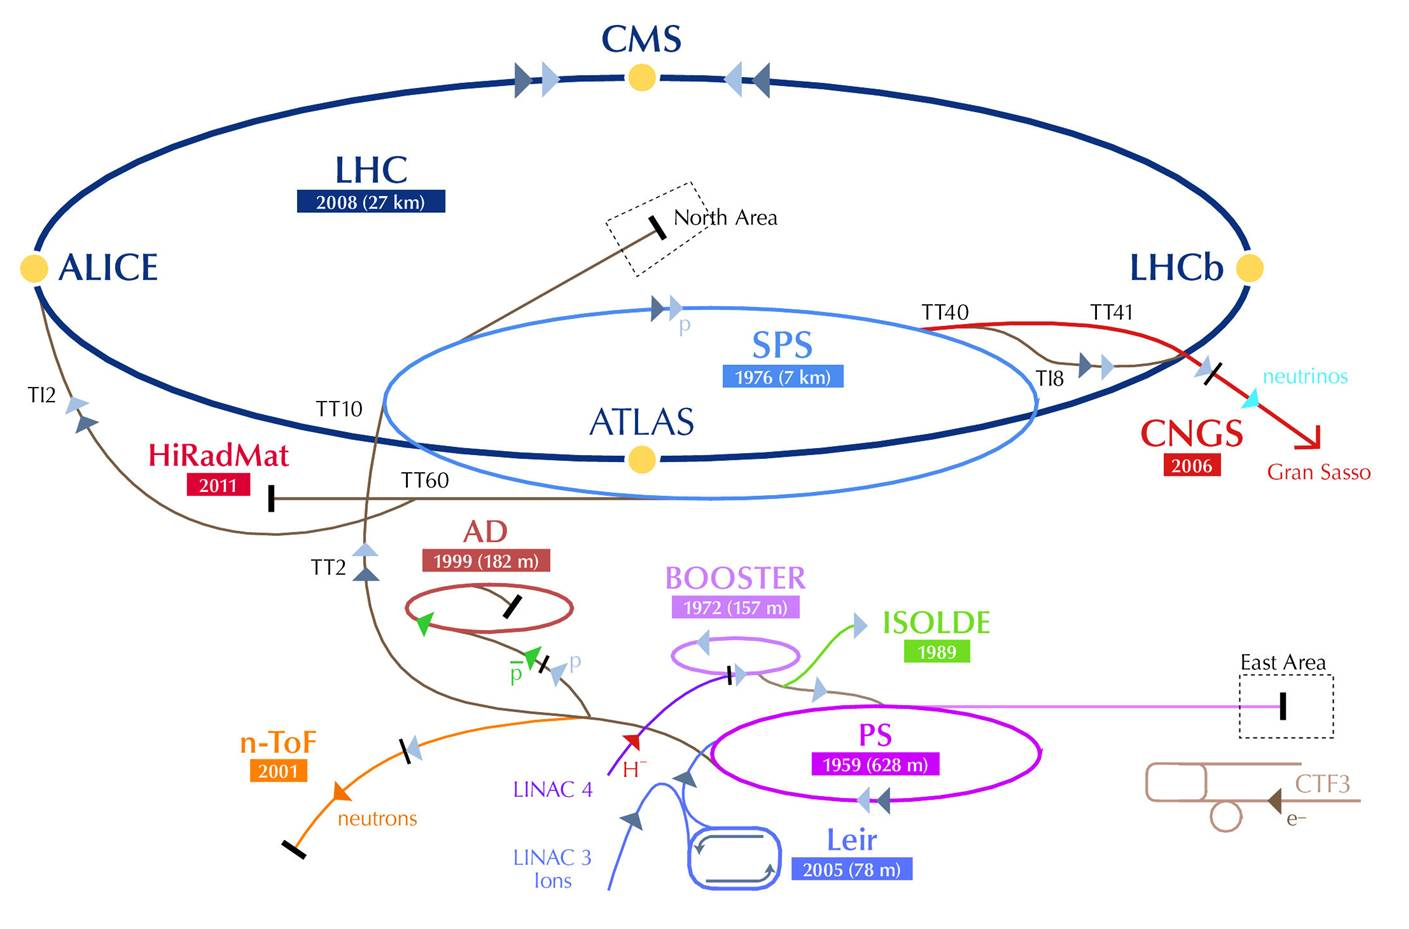
\includegraphics[width=0.8\textwidth]{ATLASdetector/Figures/CERN_Accelerator_Complex}
  \caption{Schematic view of the CERN accelerator complex.
The four main LHC experiments are shown at the interaction points.}
  \label{fig:accelerator_schema}
\end{figure}

%The LHC ring is composed of eight arcs which are \unit[2.7]{km} long, each of which contains 154 dipole magnets, whose function is to bend the beams along the circular trajectory, and 49 quadrupole magnets, that focus the beam.
%These superconducting magnets operate at a temperature of \unit[1.9]{K}, maintained by means of liquid Helium vessels.
%Eight insertions are placed in between the arches.
%Each insertion has a specific role that characterizes its design.
%These can be injection, beam dumping, beam cleaning, or ``physics'', i.e.
%make the beams collide within an experiment.

%Maybe move this to the end of ATLAS detector, with luminosity measurement
Besides its high energy, the LHC also outperforms previous accelerators in the delivered luminosity.
The instantaneous luminosity $\InstLumi$ is defined as:

\begin{equation}
  \InstLumi = \frac{n_{b} f_{r} n_{1} n_{2}}{2\pi \Sigma_{x} \Sigma_{y}}~,
  \label{eq:InstLumiDefinition}
\end{equation} 
where $n_{1}$ and $n_{2}$ are the bunch populations (number of protons per bunch) in beams~1 and~2 respectively, $f_{r}$ is the revolution frequency of the LHC, $n_{b}$ are the number of bunch pairs colliding in each revolution, and $\Sigma_{x}$ and $\Sigma_{y}$ characterize the horizontal and vertical convolved beam widths.

The event rate of a certain process can be obtained as the product of the process \xsec\ and the instantaneous luminosity:

\begin{equation}
  \frac{dN}{dt} = \InstLumi \times \sigma~.
  \label{eq:EventRat}
\end{equation}

%This rate is then directly proportional to the the frequency $f_{r}$, the number of bunches $n_{b}$ and the number of particles in the two bunches $n_1$,$n_2$, and inversely proportional to the beam \xsec\.
The instantaneous luminosity at the ATLAS collision point is measured by dedicated subdetectors that are described in section~\ref{sec:LuminosityMeasurement}.
In 2012, the LHC reached a peak luminosity of $\unit[7.7\times 10^{33}]{cm^{-2}s^{-1}}$, which is more than half the design luminosity.
Table~\ref{tab:accelerator_parameters} shows the relevant parameters for the accelerator performance.

\begin{table}[!tb]
  \small
  \centering
  \begin{tabular}{l l l l l}
    \toprule
    \toprule
    Parameter & Design value & 2010 & 2011 & 2012 \\
    \midrule
    Beam energy (\tev) & 7 & 3.5 & 3.5 & 4 \\
    Beta function $\beta^*$ (m) & 0.55 & 2.0/3.5 & 1.5/1.0 & 0.6 \\
    Max. num. bunches/beam & 2808 & 368 & 1380 & 1380 \\
    Max. num. protons/bunch & $1.15\times10^{11}$ & $1.2\times10^{11}$ & $1.45\times10^{11}$ & $1.7\times10^{11}$ \\
    Bunch spacing (ns) & 25 & 150 & 75/50 & 50 \\
    Peak luminosity ($\unit {cm^{-2}s^{-1}}$) & $1\times10^{34}$ & $2.1\times10^{32}$ & $3.7\times10^{33}$ & $7.7\times10^{33}$ \\
    Emittance $\epsilon_n$ ($\unit{\mu rad}$) & 3.75 & 2.0 & 2.4 & 2.5 \\
    Max. $\langle \mu \rangle$ & 19 & 4 & 17 & 37 \\
    \bottomrule
    \bottomrule
  \end{tabular}
  \caption{Overview of the parameters for the LHC performance comparing the design values with their time evolution during the first long run operation in 2010-2013.}
  \label{tab:accelerator_parameters}
\end{table}

Due to the high frequency of collisions and the high density of the bunches necessary to achieve such a high luminosity, there is a non-zero probability that several events, originating from different \pp\ collisions, may occur simultaneously. These events are referred to as \textit{\pileup} and are categorized as in-time or out-of-time \pileup. In-time \pileup\ events are caused by additional interactions of protons in the same bunch collision. The out-of-time \pileup\ occurs when traces from an event in a different bunch-crossing are recorded. The mean number of interactions per bunch crossing $\langle \mu \rangle$, which is taken as measure of the \pileup\ activity, is shown in figure~\ref{fig:ATLAS_mu}.

Integrating the instantaneous luminosity over the accelerator active time (a ``fill'', when stable beams are kept colliding) the integrated luminosity is obtained, relating the total number of produced events $N_{\rm tot}$ to the \xsec:

\begin{equation}
  N_{\rm tot} = \sigma \int{\InstLumi~dt}~.
  \label{eq:IntegLumiDefinition}
\end{equation}


In 2010 ATLAS collected about $\unit[45]{pb^{-1}}$ of $\pp$ collision data at $\sqrt{s} = \unit[7]{\tev}$, and in 2011 it reached about $\unit[5]{fb^{-1}}$ at the same \com\ energy.
During 2012, the last year of data taking before the long shutdown,\footnote{LHC terminated the first phase of the $\pp$ program at the end of 2012, operated proton-heavy ion collisions for two months at the beginning of 2013 and then stopped for what is called the first ``long shutdown''.
During these two-years the accelerator and the experiments underwent substantial maintenance and upgrade works, in order to be re-operated in 2015 with higher performance at a higher \com\ energy for particle collisions.}
ATLAS collected about $\unit[20]{fb^{-1}}$ of $\pp$ collision data at $\sqrt{s}=\unit[8]{\tev}$.
Figure~\ref{fig:ATLAS_lumi} shows the luminosity recorded by ATLAS during stable beam conditions.
The difference with respect to the delivered luminosity is due to Data AcQuisition (DAQ) inefficiencies.
Of the recorded luminosity, only a part is usable for analysis, which is referred to as ``good data'', i.e.
the data that satisfy Data Quality (DQ) requirements assessed after reprocessing (see section~\ref{sec:DataQuality}).

\begin{figure}[tb!]
  \centering
    \begin{subfigure}[b]{0.49\textwidth}
  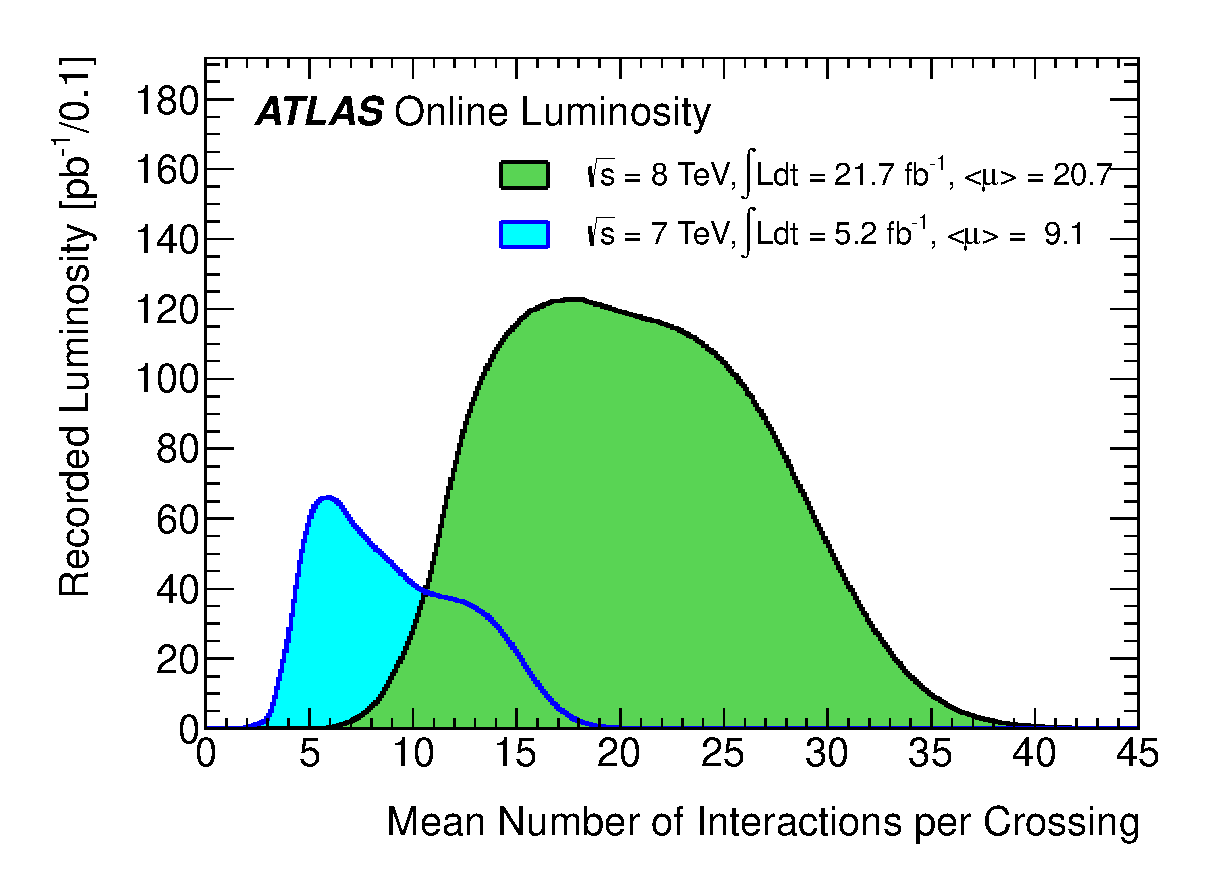
\includegraphics[width=\textwidth]{ATLASdetector/Figures/mu_2011_2012-dec}
  \caption{ }
    \label{fig:ATLAS_mu}
    \end{subfigure}
    \begin{subfigure}[b]{0.49\textwidth}
      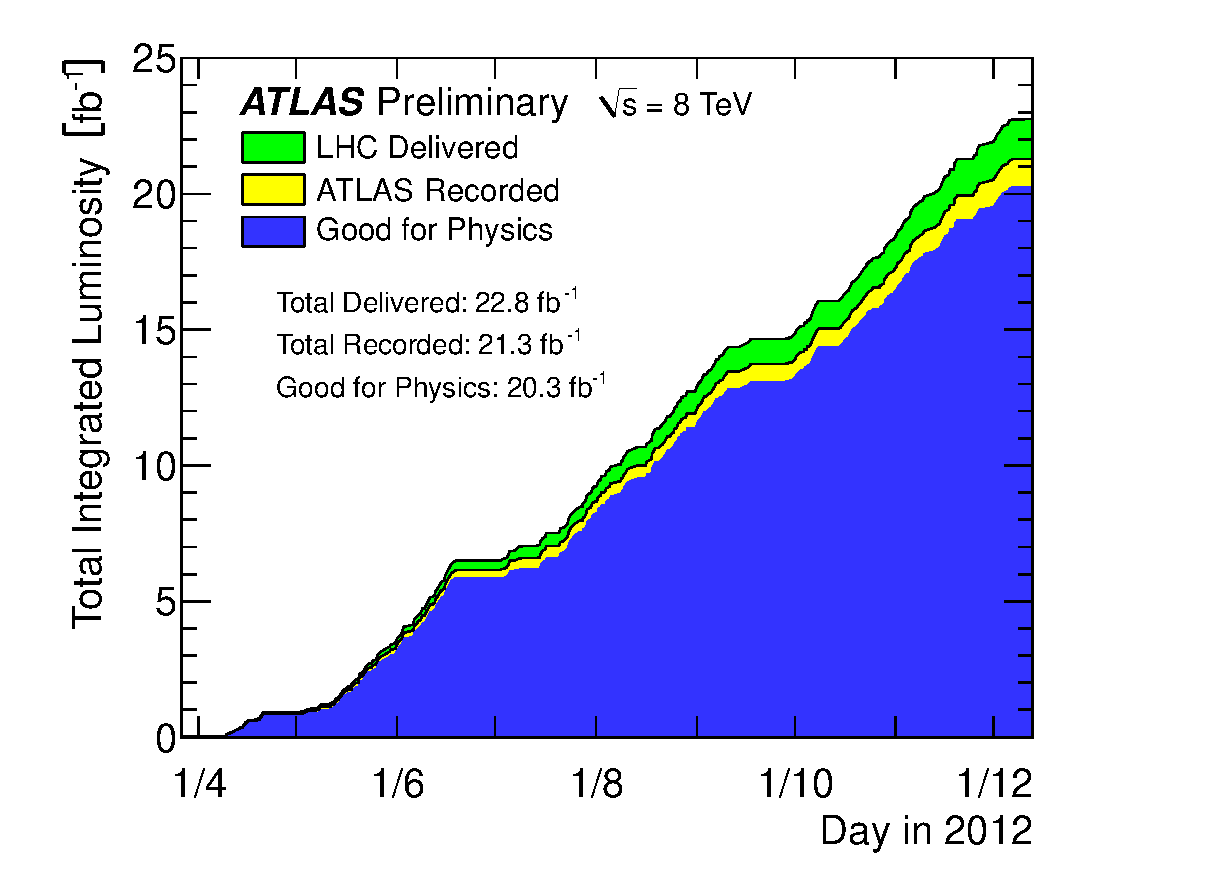
\includegraphics[width=\textwidth]{ATLASdetector/Figures/intlumivstime2012DQ}
      \caption{}
    \label{fig:ATLAS_lumi}
    \end{subfigure}
  \caption{(a)  Mean number of interactions per beam crossing during the 2011 and 2012 LHC runs.
   (b) Total integrated luminosity versus time delivered by the LHC to ATLAS (in green), recorded by the experiment (in yellow) and selected as “good data” for analysis (in blue) for $\pp$ collisions $\sqrt{s}=\unit[8]{\tev}$ in 2012. 
}
\end{figure}

%%%%% Pile-up, has to be mentioned but this section is poor and I'm not sure it belongs here
%In order to increase the luminosity LHC operates with a high number of protons per bunch as well as a high number of bunches per beam and reduces the inter-bunch latency time. This overall defines a set of challenges that physics analysis will face associated to the high luminosity. Even at the detector design stage, the high frequency of collision environment foreseen influenced the choice of radiation resistance material for the experiment subsystems. Concerning directly the physics instead, the main problematic is pile-up.
%Pile-up events are distinguished between in-time and out-of-time pile-up. The first ones come from the multiple inelastic collisions of protons in the same bunch, as if we consider a \xsec\ of 80 mb at the nominal luminosity of 1034 cm−2s−1 the number of events per second will be something like a billion. This translates, at a collision frequency of one crossing every 25 ns, to about 20 interactions per crossing that will be detected simultaneously. A useful observable to estitage in-time pile-up is the number of reconstructed primary vertices (see Section 4.2). In addition, on the other hand, the inter-bunch time interval is so short that the electronics reading the detector might not keep up with the frequency of collisions, leading to the cumulation of events that happened in different beam crossings. This is the effect we refer to as out-of-time pile-up, and a good estimator for it is the average number of $\pp$ interactions per bunch crossing at the time of the event, < μ >,n-time and out-of-time pile-up. The first ones come from the ) nf
%with L being the average instantaneous luminosity over a time period ∆t ≫ 600 ns. The maximum values reached by the variable < μ > during the three years of data taking are reported in Table 2.1
%
%\begin{figure}[!ht]
%  \centering
%     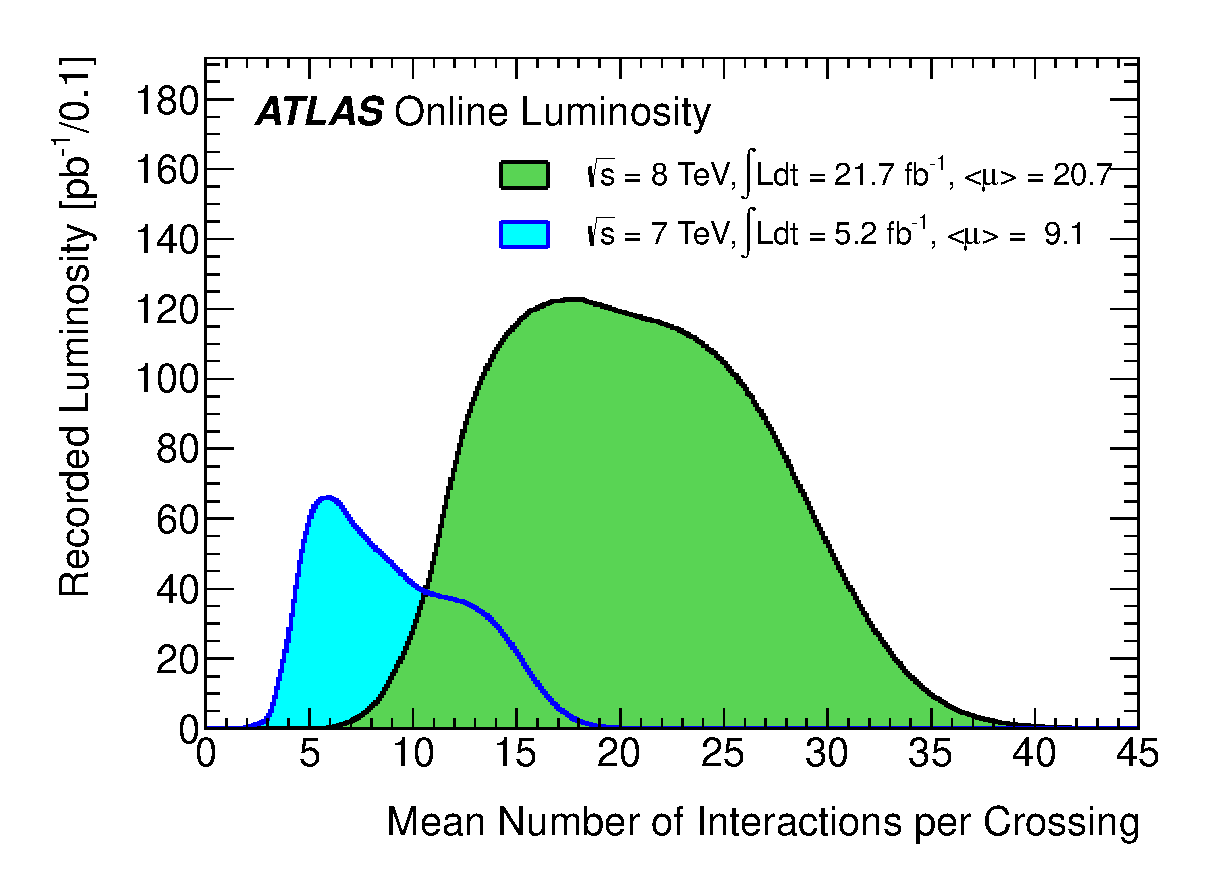
\includegraphics[width=\textwidth]{ATLASdetector/Figures/mu_2011_2012-dec}
%     \caption{Mean number of interactions per beam crossing during 2011 and 2012 LHC runs, where $\mu = \InstLumi \times \sigma_{inelastic}/f_{r}$.}
%  \label{fig:ATLAS_pileup}
%\end{figure}

\section{The ATLAS experiment} %%%%%%%%%%%%%%%%%%%%%%% ATLAS
\label{sec:ATLAS}
ATLAS (A Toroidal LHC ApparatuS) \cite{Aad:2008zzm} is a general purpose experiment aimed at exploring a vast range of physics scenarios and designed to measure the particles produced in $\pp$ collisions at the LHC at unprecedented energies and instantaneous luminosities.
It is the biggest detector of its kind ever built (about \unit[46]{m} long, \unit[25]{m} wide and weights \unit[7000]{t}) and it is characterized by a full coverage of the space around the $\pp$ interaction point and complete containment of the particles produced in the collision. %Mentira
Different subsystems are layered concentrically one after the other, as shown in figure~\ref{fig:ATLASsketch}, each devoted to the measurement of different properties for different types of particles.
The subdetectors are grouped into three main systems:
\begin{itemize}
  \item The Inner Detector, immersed in a solenoidal magnetic field, constitutes a tracking system used to identify and measure the momenta of charged particles and to identify the interaction vertices and the displaced vertices.
  \item The Calorimeters are used to identify and measure the energy of neutral and charged particles.
They are designed to stop most types of particles, except for muons and neutrinos.
  \item The Muon Spectrometer is used to detect and measure the properties of muons.
Because muons minimally interact with the other parts of the detector and have long lifetimes, they are identified and measured in the outermost detector layer.
\end{itemize}
%Furthermore, ATLAS uses a solenoidal magnetic field in order to bend the particle trajectories in the inner detector, and a toroidal magnetic field for the muon spectrometer.

\begin{figure}[!tb]
  \begin{center}
    \includegraphics[width=\textwidth]{ATLASdetector/Figures/ATLAS_Detector.eps}
  \end{center}
  \caption{Drawing of the ATLAS detector showing the different subdetectors and the magnet systems.}
  \label{fig:ATLASsketch}
\end{figure}

\subsection{Coordinate system}
\label{subsec:Coordinate_system}

The ATLAS reference system is a cartesian right-handed coordinate system with origin at the nominal interaction point (IP) in the center of the detector.
The $X$-axis points from the IP to the center of the LHC ring, the $Y$-axis points upwards and the positive $Z$-axis is defined along the anti-clockwise beam direction.
The azimuthal angle $\phi$ is measured around the beam axis, ranging between $-\pi$ and $+\pi$ with respect to the $X$-axis.
The polar angle $\theta$ is measured with respect to the $Z$-axis and ranges between 0 and $\pi$.
Since the momentum of the colliding partons along the $Z$-axis is unknown, it is useful to define the transverse component of variables of interest, like energy and momentum, defined as the projection on the $XY$ plane, which are boost-invariant along the $Z$-axis:
\begin{equation}
  \et = E \sin\theta, \qquad \pt = p \sin\theta.
  \label{eq:transverse_components}
\end{equation}
Another common variable used at hadron colliders to describe the polar distribution and preferred to the simple polar angle $\theta$ is the rapidity $y$:
\begin{equation}
  y \equiv \frac{1}{2}\ln \left(\frac{E+p_{Z}}{E-p_{Z}}\right),
  \label{eq:rapidity_definition}
\end{equation}
which, for vanishing particle mass, is equal to the pseudorapidity $\eta$:
\begin{equation}
  \eta \equiv -\ln{\left(\tan{\frac{\theta}{2}}\right)}.
  \label{eq:pseudorapidity_definition}
\end{equation}

The advantage of both variables over $\theta$ is that rapidity differences $\Delta y$ are boost-invariant along the $Z$-axis, as well as pseudorapidity differences $\Delta \eta$ for massless particles.
The pseudorapidity is usually preferred to the rapidity as it does not require knowing the particle's mass but only its polar position.
The distance between two particles is often referred to in terms of $\Delta R$:
\begin{equation}
  \Delta R \equiv \sqrt{(\Delta\eta)^2+(\Delta\phi)^2}~.
  \label{eq:deltaR}
\end{equation}

ATLAS covers the pseudorapidity regions up to $\abseta < 4.9$.
However, physics analyses typically consider objects restricted to the pseudorapidity region $\abseta < 2.5$.


\subsection{Magnet system}
    \label{subsec:Magnets}
The measurement of charged particles' momenta is based on their deflection in a magnetic field.
The magnet system \cite{MAGtdr} represents a particular characteristic of the ATLAS experiment which sets it
apart in the panorama of high energy physics.
It is composed of four large superconducting magnets
designed to provide a field mostly orthogonal to the particle trajectory:
a central solenoid and three open-air toroids as shown in figure~\ref{fig:DETmagnets}.
%This hybrid solution has the advantage of extending the pseudorapidity coverage of the muon spectrometer, 
%and having no magnetic field inside the calorimeters in order not to degrade their performance.

\begin{figure}[!ht]
\begin{center}
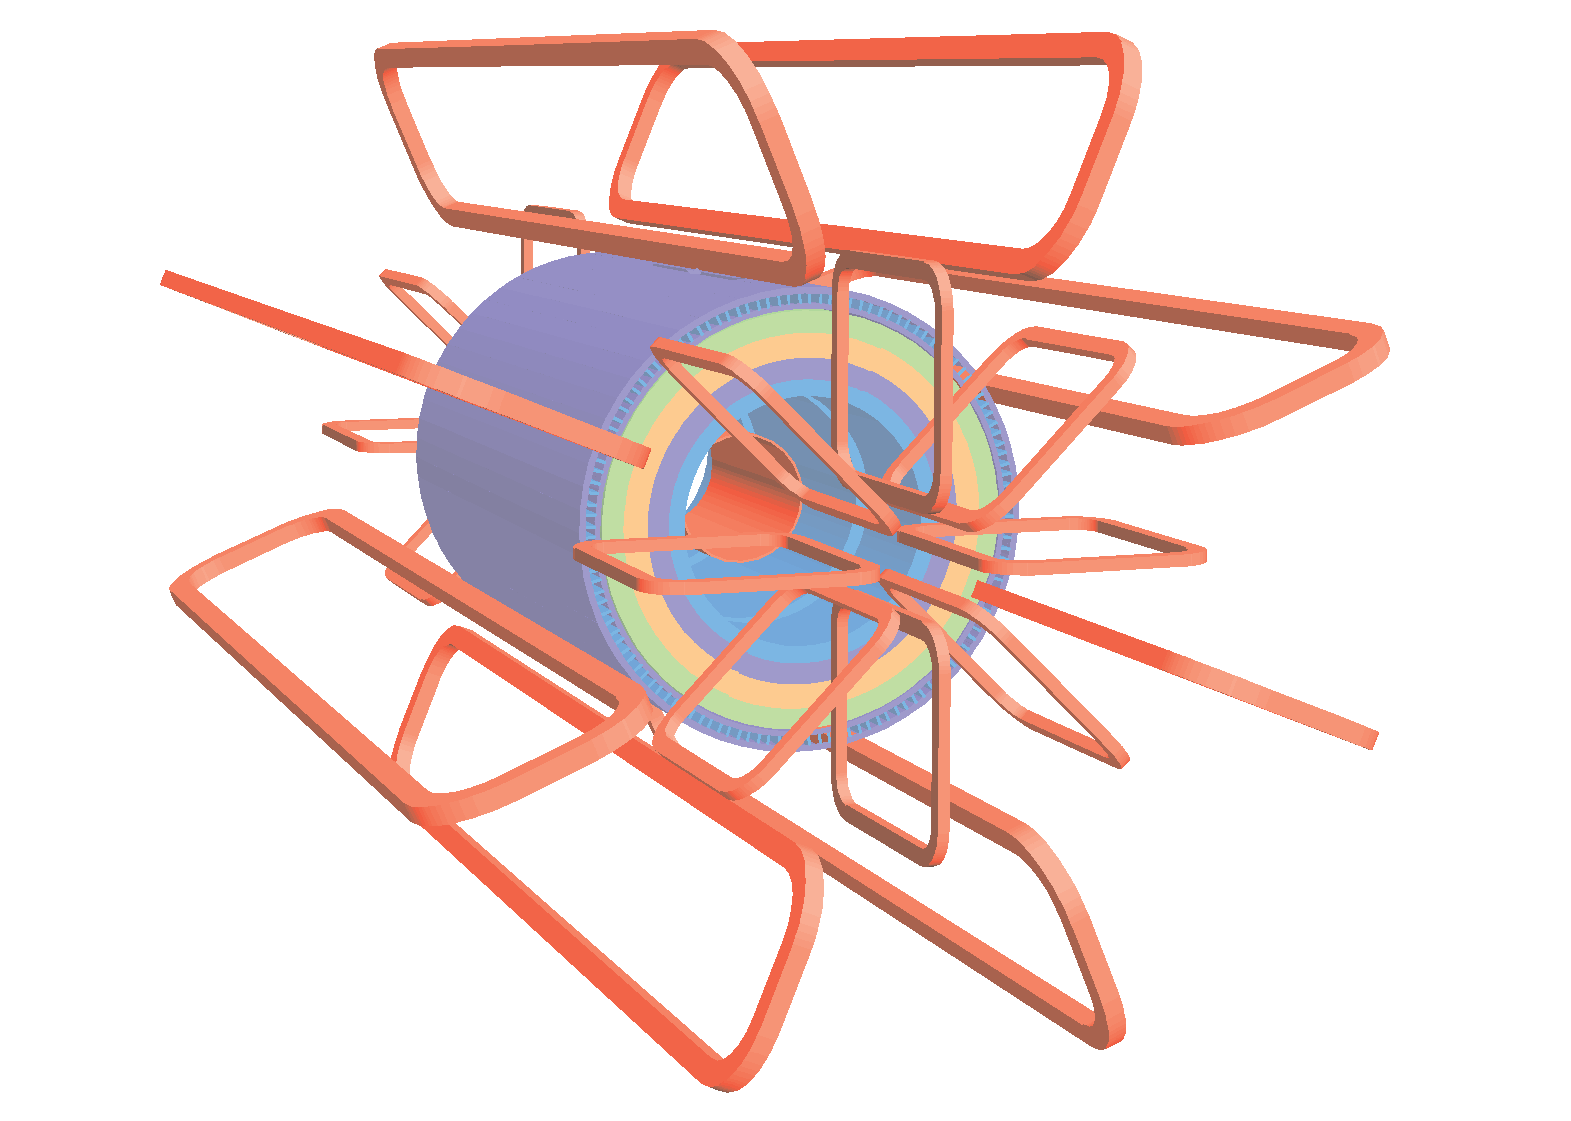
\includegraphics[width=0.7\textwidth]{ATLASdetector/Figures/ATLcoilGeom.eps}
\caption{Schematic view of the ATLAS magnet system: three external toroids and the central solenoid enclosed by the calorimeters.}
\label{fig:DETmagnets}
\end{center}
\end{figure} 

% from Frank: "Given your emphasis on not having a B-field inside the calorimeters, I'm wondering what's done with the return field from the solenoid?"
The central solenoid surrounds the Inner Detector and provides a magnetic field parallel to the beam axis bending charged particles in the $\phi$ direction.
%The CS' length is \unit[5.3]{m} centered at the interaction point and it has a radius of \unit[2.5]{m}.
 At the interaction point the value of the magnetic field is \unit[2]{T} and it remains constant in the radial direction.
As the distance from the interaction point  increases in the $z$ direction, the field strength decreases as a result of the finite size of the solenoid.
%%The average magnetic field value is 2 T with a very stable radial profile and a  a maximum of 2.6 T in the proximity of  the magnets.
%In order to minimise the amount of material in front of the calorimeter, the solenoid and the liquid Argon calorimeter share the same cooling cryostat.

The toroid system produces the field needed by the muon spectrometer to deflect particles in the $\eta$ direction: 
two end-cap toroids at the two extremes of the detector and a 
barrel toroid centrally located around the calorimeters.
Each toroid is composed of eight independent coils equally distributed in the azimuthal plane.
The barrel toroid generates a magnetic field of \unit[3.9]{T} while the end-cap produces a field of \unit[4.1]{T}.
The choice of the ``open air" toroid configuration was made to improve the muon reconstruction performance without relying on the Inner Detector.
The toroids allow to efficiently generate the magnetic field over a large volume with a reduced amount of material.
This minimizes the amount of multiple scattering,\footnote{
Multiple scattering is defined as the electromagnetic interaction of a charged particle with the atomic structure of the medium.
The result of the interaction with the very large number of nuclei and electrons results into a random smearing of the momentum of the incoming particle.} 
which represents one of the factors limiting the muon momentum resolution.
%%limiting factor for momentum resolution at very high muon \pT.

%The end-cap toroids are rotated by  $22.5^{\circ}$ with respect to the central barrel in order to improve the overlap of the respective magnetic fields and achieve a higher uniformity.
%Both magnets are helium-cooled to a temperature of \unit[4.5]{K} in order to reach the super-conducting state.

\subsection{Inner detector}
\label{subsec:InnerDetector}

The Inner Detector (ID) \cite{IDtdr} is the subdetector closest to the IP.
 It provides tracking of charged particles arising from collisions, allowing for vertex reconstruction and measurement of track momenta in the range $\abseta<2.5$.
The detector design required fast response electronics, good radiation resistance and reducing to a minimum the amount of material to be placed in front of the calorimeters to avoid degrading the energy measurement.
%The amount of material that makes up the ID varies between 0.5 and 2.5 $X_0$ depending on the pseudorapidity region, most of it coming from support equipment.
%The ID is $\unit[6.2]{m}$ long and $\unit[2.1]{m}$ in diameter, covering a range $\abseta<2.5$.
It is divided in three different concentric subdetectors, named (increasing in distance with respect to the IP) pixel, semi-conductor tracker (SCT) and transition radiation tracker (TRT).
Figure~\ref{fig:InnerDetector} shows a cut-away view of the ATLAS ID.
\begin{figure}[!ht]
  \centering
      \includegraphics[width=\textwidth]{ATLASdetector/Figures/InnerDetector.eps}
  \caption{Cut-away view of the ATLAS Inner Detector.}
  \label{fig:InnerDetector}
\end{figure}


\subsubsection{Pixel}
    \label{subsubsec:Pixel}

    The pixel detector is the innermost part of the ID and measures charged particles using radiation-hard silicon sensors (pixels).
It covers the region $\abseta < 2.5$ and is composed of three cylindrical layers in the barrel region, 
%each of them distant from the beam by \unit[50.5]{mm}, \unit[88.5]{mm} and \unit[122.5]{mm} respectively, 
and of three concentric discs in the end-cap region.
%, at a distance from the center of the detector of \unit[49.5]{mm}, \unit[58.0]{mm} and \unit[65.0]{mm} respectively.
Each silicon pixel has a size of $\unit[50 \times 400]{\mu m^2}$ and is $\unit[250]{\mu m}$ thick, resulting in total $\approx 80.4$ million readout channels to achieve a very fine granularity.
The precision is of $\unit[10]{\mu m}$ in the $R-\phi$ plane, and $\unit[115]{\mu m}$ in Z and R in the barrel and end-cap region, respectively.
The very first layer is called B-layer and, thanks to its position really close to the IP, \unit[50.5]{mm} away, allows for the reconstruction of secondary vertices associated with the production of long-lived particles such as $b$-hadrons.
This information is very useful to identify jets originating from the fragmentation of $b$-quarks.

\subsubsection{Semiconductor tracker}
    \label{subsubsec:SCT}

The Semiconductor Tracker (SCT) is the middle part of the ID and is a silicon microstrip detector.
It is composed of a barrel, with four layers of silicon microstrip detectors, and two endcaps, each with nine disks, covering the range $\abseta < 2.5$.
The minimal SCT unit, the module, is a pair of single-sided silicon microstrip sensors mounted back-to-back, containing 768 microstrips.
%It has an active area of $\unit[6.36\times6.40]{cm^2}$ and contains 768 microstrips with a $\unit[80]{\mu m}$ width.
The back-to-back sensors are mounted with a \unit[40]{mrad} ``tilt'' angle, so that the crossing point of the strips on both sides is used to determine the space point position.
In the barrel, silicon strips are arranged parallel to the beam line, while in the disks, the strips are oriented radially.
The spatial resolution achieved is $\unit[17]{\mu m}$ in $R-\phi$ and $\unit[580]{\mu m}$ in $Z$ ($R$) in the barrel (end-cap) region.

\subsubsection{Transition radiation tracker}
    \label{subsubsec:TRT}

The Transition Radiation Tracker (TRT) is the outermost part of the ID.
It consists of \unit[4]{mm}-diameter gaseous straw tubes interleaved with transition radiation material, enabling tracking for $\abseta<2$.
%Each straw contains a $\unit[30]{\mu m}$ gold-covered tungsten anode wire and is filled with a gas mixture of 70\% Xe, 20\% $\text{CO}_2$ and 10\% $\text{CF}_4$.
The space between the tubes is filled with plastic material (polyethylene) in order to produce the transition radiation.
The emission of photons depends on the Lorentz boost $\gamma$ $(E/m)$ of the particles and, in the energy range of interest, is present only for electrons.
The TRT is only segmented in $R-\phi$, and it provides a resolution of $\unit[130]{\mu m}$ per straw.
%This subdetector mainly contributes to electron identification~\cite{Aad:2011mk}.

\subsubsection{Inner detector combined performance}
The relative precision of the three subdetectors is comparable so that no single measurement dominates the momentum resolution.\footnote{The lower intrinsic resolution of the TRT is compensated by the higher number of hits per track and by the possibility of analyzing a longer track segment.}
%This redundancy also guarantees high efficiency even in case a part of one of the subdetector is malfunctioning.
Using the combined information from the three subdetectors, the transverse momentum resolution measured with cosmic muons~\cite{Aad:2010mr} is:

\begin{equation}
  \frac{\sigma_{\pt}}{\pt} = 1.6 \% \oplus \frac{0.053 \%}{\gev}\times \pt, 
  \label{eq:IDresolution}
\end{equation}

%\noindent 
%where $P_{1} = \unit[1.6]{\%}$ and $P_{2} = \unit[5.3\times 10^{-2}]{\GeV^{-1}\%}$.
This translates in a resolution of $1.6\%$ for tracks with $\pt\sim \unit[1]{\GeV}$ and of about 50\% for $\pt\sim \unit[1]{\TeV}$.


\subsection{Calorimeters}
    \label{subsec:Calorimeters}

The ATLAS calorimeters surround the ID, covering the full $\phi$ space and the range $\abseta<4.9$.
%, extending radially $\unit[4.25]{m}$.
They are designed to stop and contain most of the particles from the interaction, except for muons and neutrinos.
The calorimeters are divided into a central barrel part and two symmetric end-caps, as shown in figure~\ref{fig:CalorimetersSchema}.
In the acceptance region covered by the ID the electromagnetic calorimeter has very fine segmentation for precise measurement of photons and electrons.
The hadronic and forward calorimeters have coarser segmentation but still allow a precise measurement of jet kinematics as well as sufficient pseudorapidity coverage for the missing transverse energy calculation.


\begin{figure}[!ht]
  \centering
      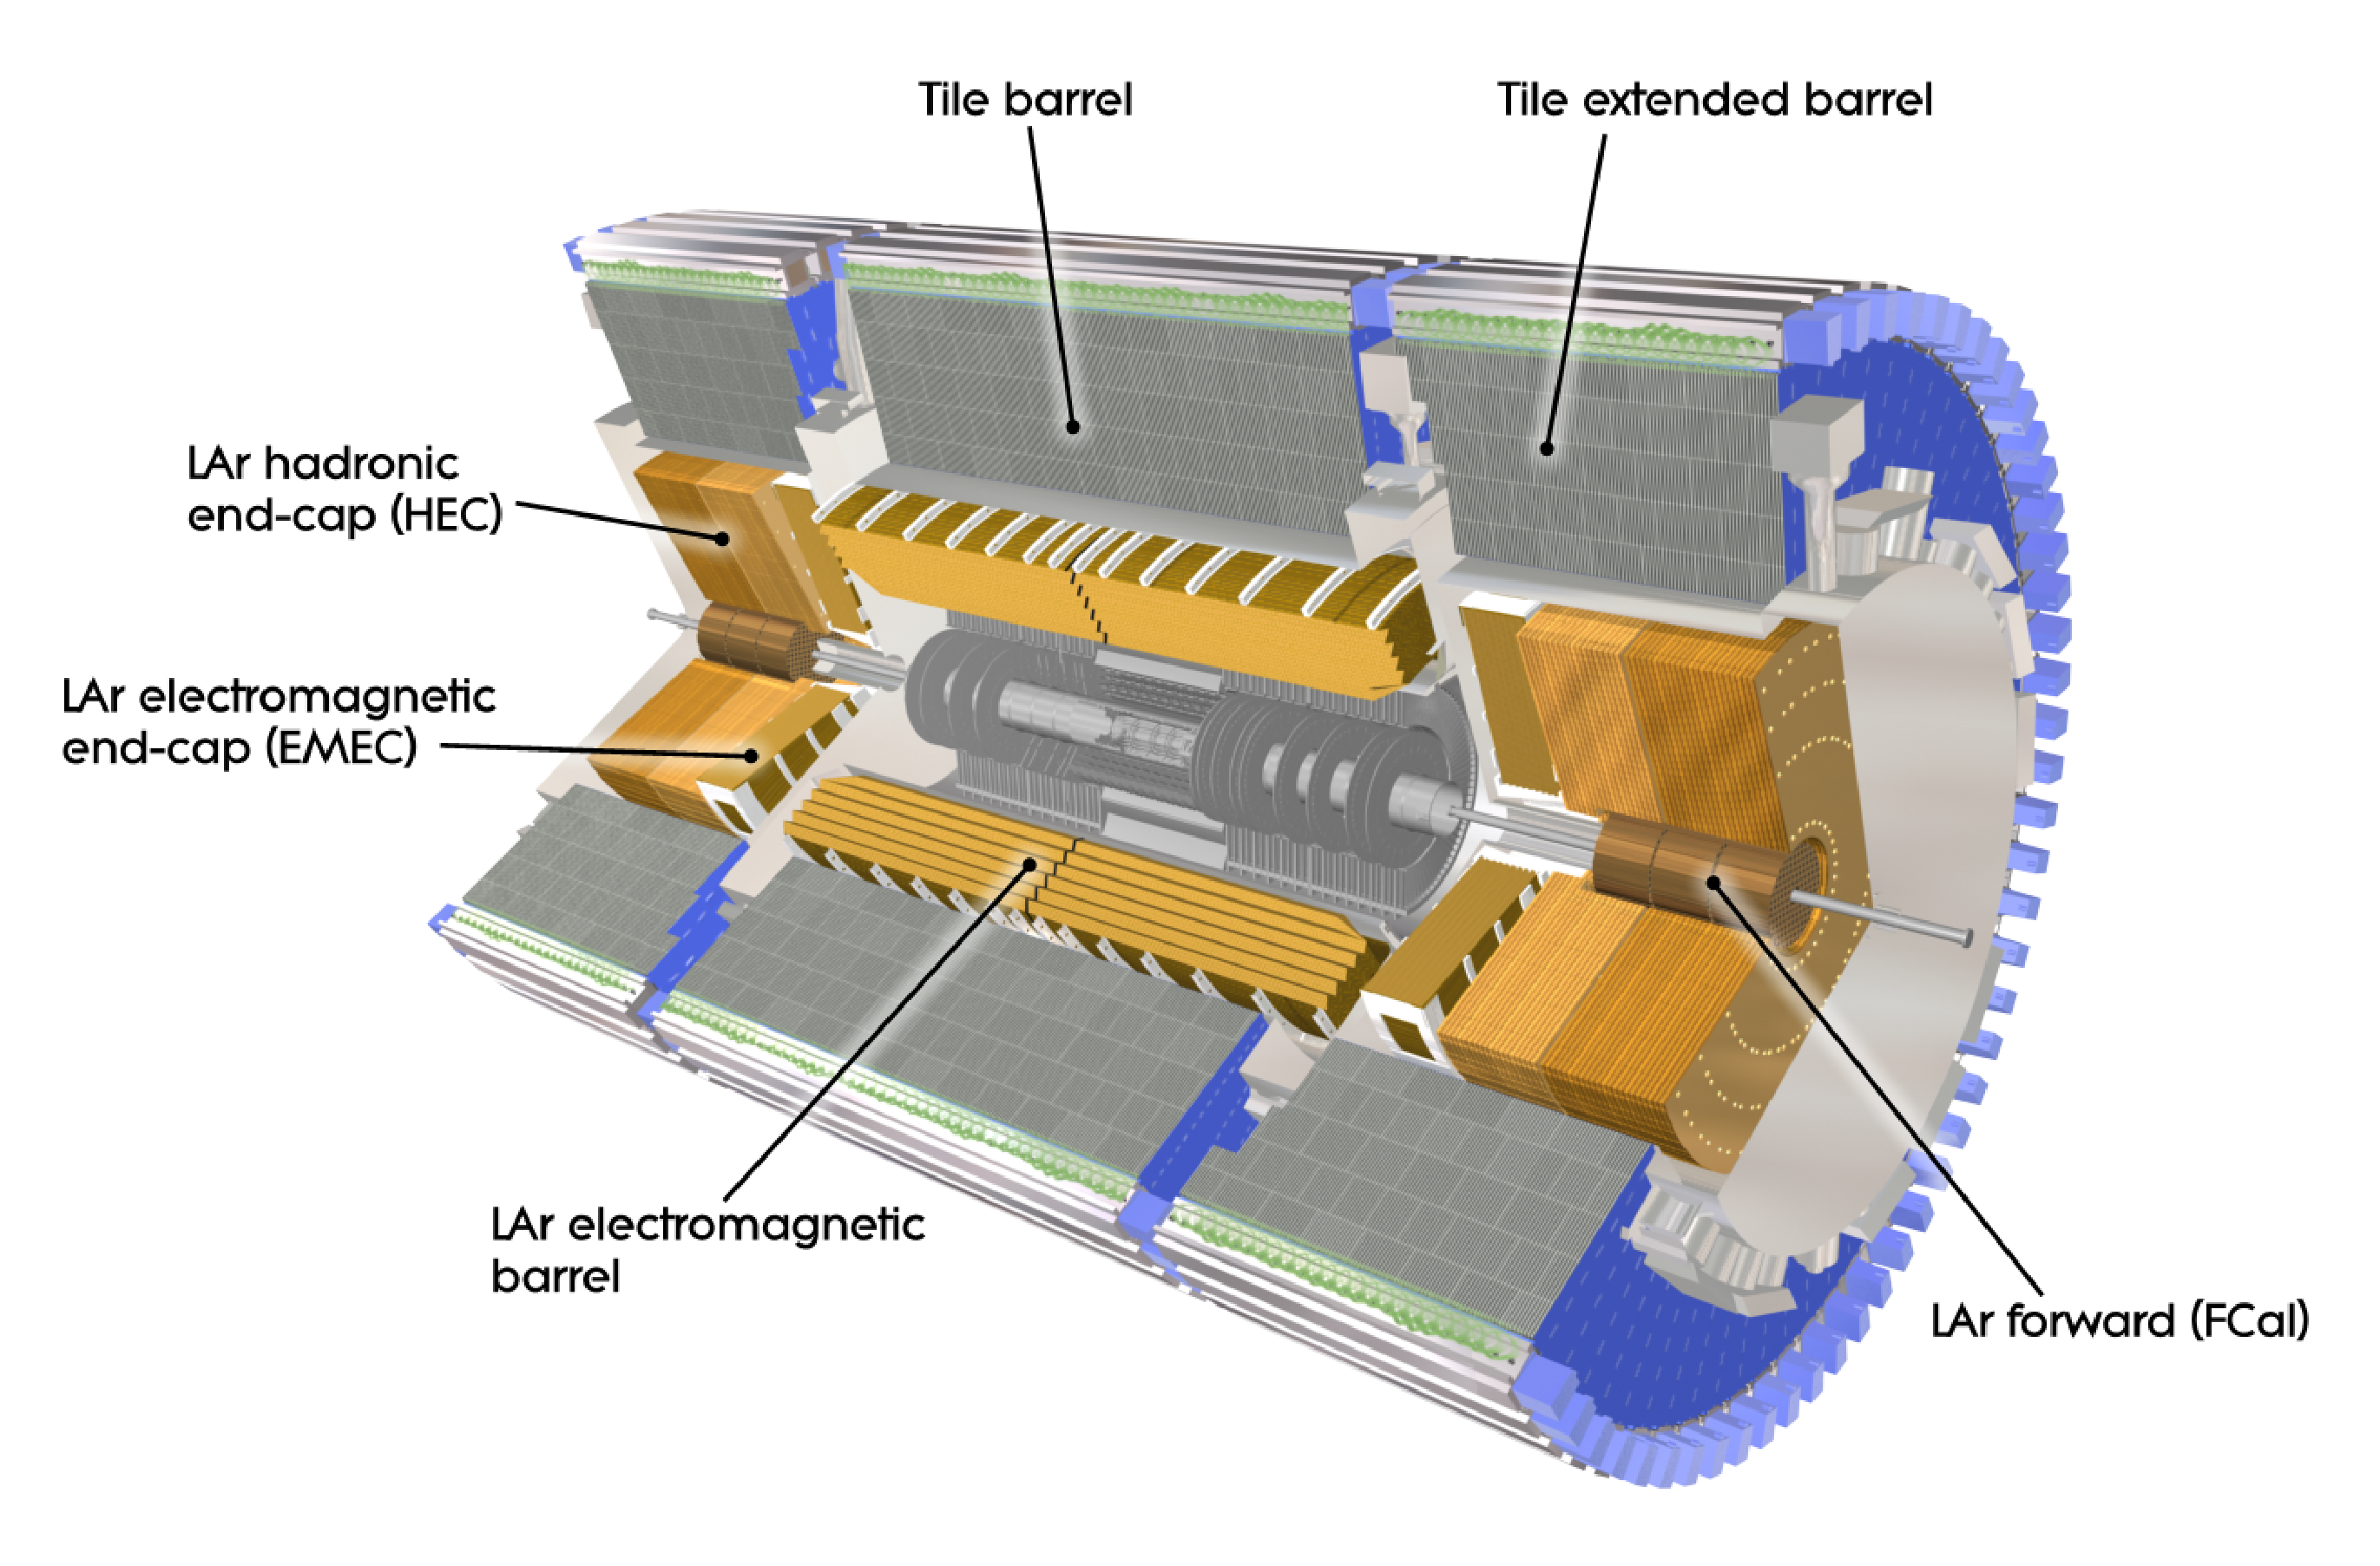
\includegraphics[width=\textwidth]{ATLASdetector/Figures/Calorimeter.eps}
  \caption[Schematic view of the ATLAS calorimeter system.]{Schematic view of the ATLAS calorimeter system.}
  \label{fig:CalorimetersSchema}
\end{figure}

\subsubsection{Electromagnetic calorimeter}
\label{subsubsec:LAr}
The electromagnetic calorimeter (ECAL)\cite{LARtdr} is a sampling calorimeter that uses liquid argon (LAr) as active material and lead plates as absorber.
The liquid argon solution was adopted for its intrinsic linear behavior, high ionization yield, stability and resistance to radiation.
The lead plates have a characteristic ‘accordion’ shape and are oriented in the radial direction.
This allows a complete symmetric coverage without cracks in the azimuthal direction.
High voltage is applied between absorber plates to collect the ionization electrons from the interaction in the liquid argon as well as to produce the signal amplification.
%The electric signal is read from shaped cathodes in the plates through capacitive coupling.
The ECAL barrel covers the range $\abseta < 1.475$, while the end-caps extend the reach to $1.375< \abseta < 3.2$.

The ECAL barrel is segmented in order to create three longitudinal sections with very different depths and cell structure in the $\eta-\phi$ plane.
Figure~\ref{fig:LArModule} shows the geometry of one module of the calorimeter.

The first layer, with a thickness of 4.3 radiation lengths ($X_0$), is finely segmented in $\eta$ with thin readout strips of $\Delta \eta \times \Delta \phi = 0.0031 \times 0.098$, in order to measure precisely the direction in pseudorapidity of the particles.
The strip layer is of particular importance for photon and electron identification and, combined with the information from the second layer, can be used to obtain precise information on the photon's production vertex.
The second layer, $\unit[16]{X_0}$ thick, represents most of the thickness of the calorimeter.
It is divided in towers of size $\Delta \eta \times \Delta \phi = 0.025 \times 0.025$ and provides the position measurement of the cluster.
About 95\% of the energy of the shower is deposited in a matrix of $3\times7$ towers in $\Delta \eta \times \Delta \phi$.
The third layer, just $\unit[2]{X_0}$ thick, has coarser granularity and it is used to estimate the amount of energy lost beyond the ECAL.
Towers in this region have a dimension of $\Delta \eta \times \Delta \phi = 0.05 \times 0.0245$.
In the central region an additional pre-sampler layer is present.
The information from this layer is exploited in the calibration to estimate the energy lost by the electron or photon in the passive material of the solenoid.

The total thickness of the ECAL is at least \unit[22]{$X_0$}, increasing with $\eta$ from 22 $X_0$ to 33 $X_0$ in the barrel and from 24 $X_0$ to 38 $X_0$ in the endcap.
This guarantees a full containment of electrons and photons up to energies of a few \tev.

The target energy resolution for the ATLAS electromagnetic calorimeters is~\cite{LARtdr}:
\begin{equation}
  \frac{\sigma_E}{E}=\frac{10\%}{\sqrt{E}} \oplus \frac{17 \%}{E} \oplus 0.7\%~,
  \label{eq:LAr_resolution}
\end{equation}
with $E$ measured in \gev.

\begin{figure}[!ht]
  \begin{center}
    \begin{subfigure}[b]{0.49\textwidth}
      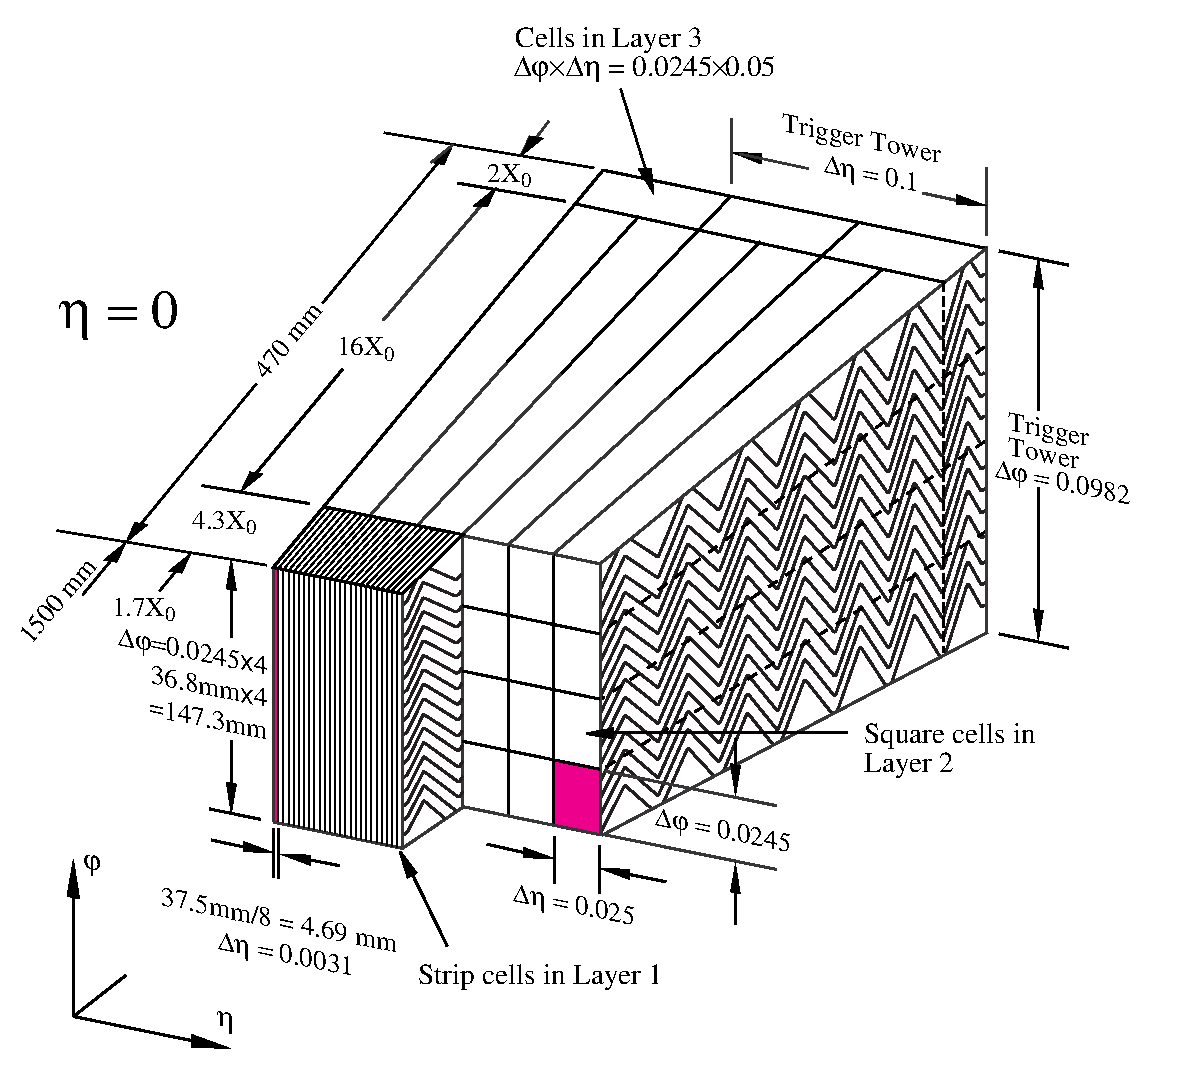
\includegraphics[width=\textwidth]{ATLASdetector/Figures/LAr_Module.eps}
      \caption{}
      \label{fig:LArModule}
    \end{subfigure}
    \begin{subfigure}[b]{0.49\textwidth}
      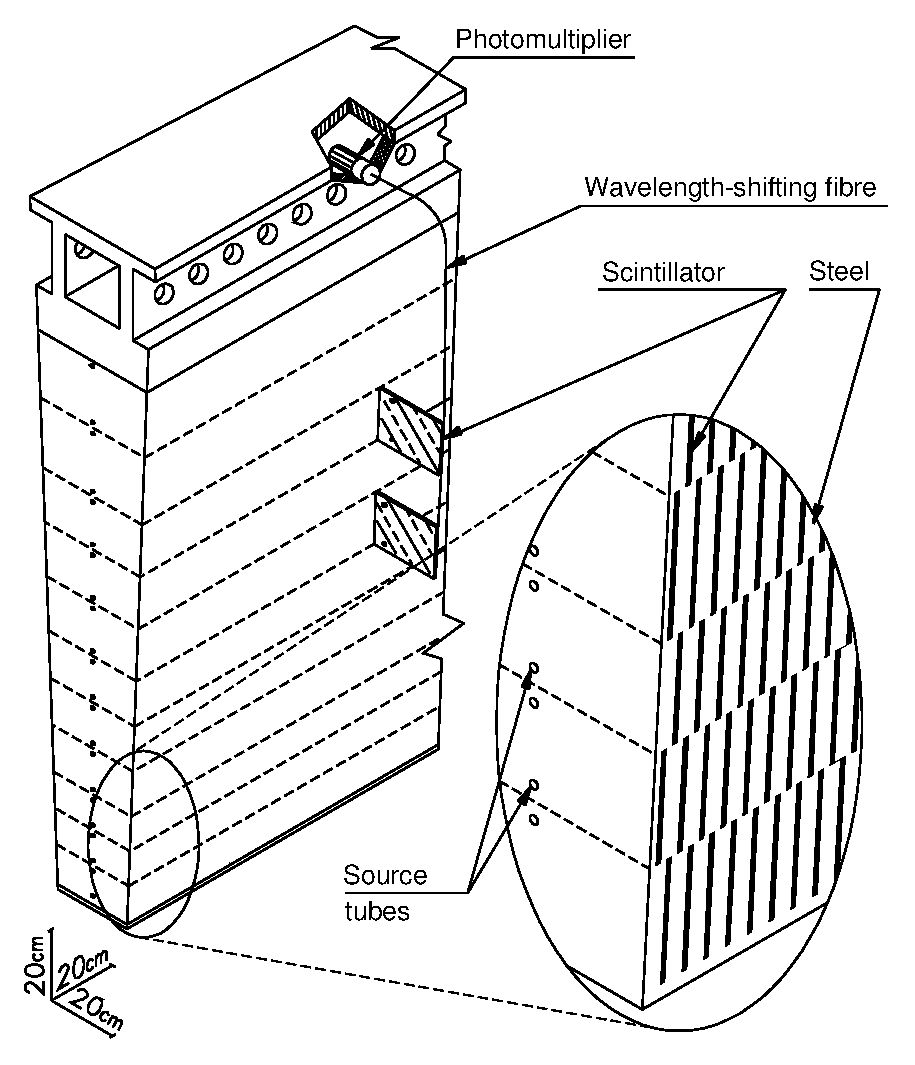
\includegraphics[width=\textwidth]{ATLASdetector/Figures/TileCal_Module.eps}
      \caption{}
      \label{fig:TileCalModule}
    \end{subfigure}
    \label{fig:CalorimeterModules}
    \caption{Schema of different modules of the ATLAS calorimeters: (a) electromagnetic calorimeter and (b) hadronic calorimeter.}
  \end{center}
\end{figure}


\subsubsection{Hadronic calorimeter}
    \label{subsubsec:TileCal}
    The ATLAS hadronic calorimeter is composed of different independent sampling ca\-lo\-ri\-me\-ters, each with its own particular technology and choice of material.
The choice was dictated by the different conditions in terms of radiation flux and performance requirements as a function of the pseudorapidity of the particles.

    In the central region the Tile Calorimeter\cite{TILEtdr}, referred to as TileCal, covers the range $\abseta < 1.7$.
%(\unit[11.4]{m} long cylinder with an inner radius of \unit[2.28]{m} and an outer radius of \unit[4.25]{m}).
    It consists of a sampling calorimeter employing steel tiles as passive material (absorber) and plastic scintillators as active material.
Figure~\ref{fig:TileCalModule} shows a schema of one TileCal module.
    TileCal is divided into a long barrel (LB, $\abseta<1.0$) and two extended barrels (EB, $0.8<\abseta<1.7$).
Both the LB and the EB are segmented into 64 modules in $\phi$, corresponding to a $\Delta\phi$ granularity of $\unit[0.1]{radians}$.
Radially, each module is further segmented into three layers, with thicknesses of approximately 1.5, 4.1 and 1.8 hadronic interaction lengths ($\lambda$) for the barrel and 1.5, 2.6 and $\unit[3.3]{\lambda}$ for the extended barrel.
%(as shown in Figure~\ref{fig:InteractionLengthCalo}).
The $\Delta\eta$ segmentation of each module is $0.1$ in the first two radial layers and $0.2$ in the third one.

Wavelength-shifting fibers coupled to the tiles on either $\phi$ edge of the cells collect the light produced and are read out by two photomultiplier tubes (PMT), each linked to one readout channel.
The readout channels are grouped into cells forming a pseudo-projective geometry in $\eta$, as shown in figure~\ref{fig:TileCalLayout}.

The transition region between the LB and the EB is supplemented with a set of special cells: 
%Furthermore, located on the inner radius surface of the extended barrel modules, 
the gap scintillators cover the region of $1.0<\abseta<1.2$ while the crack scintillators are located on the front of the LAr end-cap and cover the region $1.2<\abseta<1.6$.
%Finally, 16 Minimum Bias Trigger Scintillators (MBTS) are located on the front face of the LAr end-cap cryostat and span an $\eta$ range of $2.12<\abseta<3.85$.

\begin{figure}[!ht]
  \begin{center}
    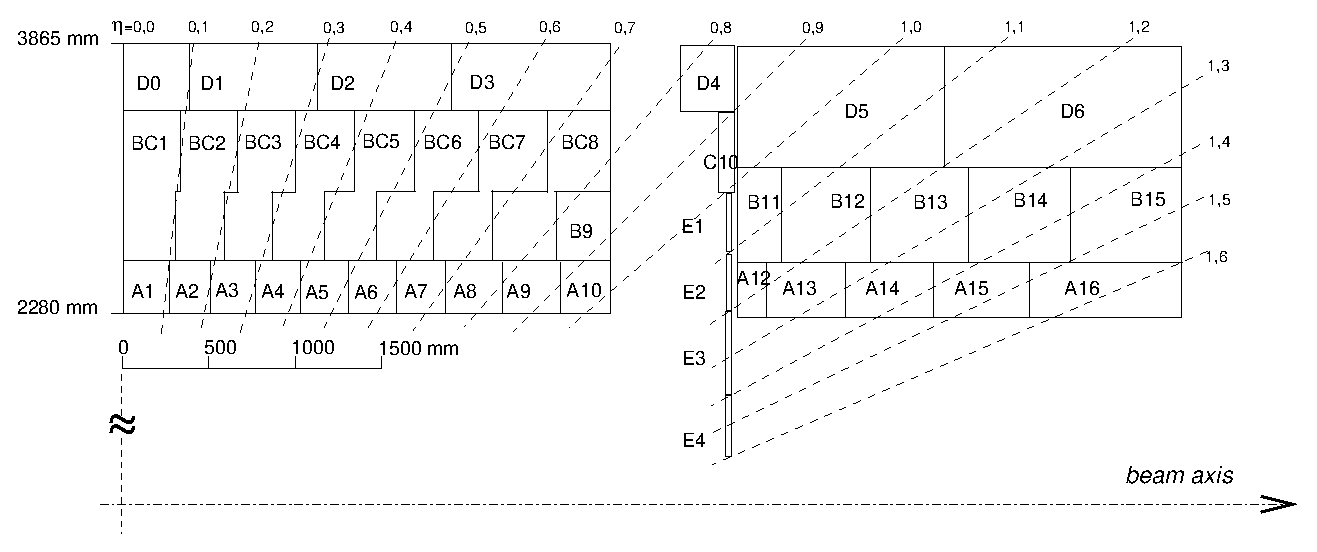
\includegraphics[width=\textwidth]{ATLASdetector/Figures/TileCal_Cells_and_Rows2}
  \end{center}
  \caption{Layout and geometry of the cells and layers in the hadronic calorimeter.}
  \label{fig:TileCalLayout}
\end{figure}

The author has contributed to performance studies of the hadronic calorimeter, and the work has been documented in appendix~\ref{chapter:TileTimingPerformance}.
\newline

The Hadronic End-Cap calorimeter (HEC) uses copper as passive material and liquid argon as active material, chosen for its radiation hardness in a region ($1.5 < \abseta < 3.2$) exposed to a significant particle flux.
  Each HEC is composed of two independent wheels with granularity varying with $\eta$.
In $1.5 < \abseta < 2.5$, $\Delta \eta \times \Delta \phi = 0.1 \times 0.1$ in the first two longitudinal layers, and $0.2\times0.1$ in the last one.
In the range $2.5 < \abseta < 3.2$, the granularity is $\Delta \eta \times \Delta \phi = 0.2 \times 0.2$ in all the three samples.

Finally, the Forward Calorimeter (FCal) covers the very forward region of pseudorapidity, $3.1 < \abseta < 4.9$, making the calorimeter system achieve its good hermeticity and minimizing the energy losses.
It is assembled with tungsten rod absorbers embedded in a copper matrix.
Between the two, a thin gap filled with liquid argon provides the active material.


\subsection{Muon spectrometers}
    \label{subsec:MuonSpectrometers}

    The most external detector system is the muon spectrometer~\cite{MUONtdr}, a combination of toroidal superconducting magnets and precision chambers providing a measurement of the momentum of muons for $\abseta < 2.7$.
    %, in addition to the measurement from the ID.
    It is also equipped with an independent trigger system used for the first event triggering stage (see section~\ref{sec:TriggerSystem}) active in the pseudorapidity region $\abseta < 2.4$.
    Four subdetectors compose the muon system: Monitored Drift-Tube (MDT) chambers, Cathode Strips Chambers (CSC), Resistive Plate Chambers (RPC) and Thin Gap Chambers (TGC).
The layout changes in the barrel and end-cap regions, and is schematically shown in figure~\ref{fig:MuonSpectrometerSchema}.
In the barrel region, chambers are arranged in three cylindrical layers around the beam axis, one layer being inside the magnet.
In the end-caps these three layers are placed perpendicular to the beam axis.
The variety of technologies used responds to the different needs of the detector (precise position and momentum measurement versus triggering and time measurement) and the large variation in particle flux from the central to the forward region.

\begin{figure}[!tb]
  \begin{center}
      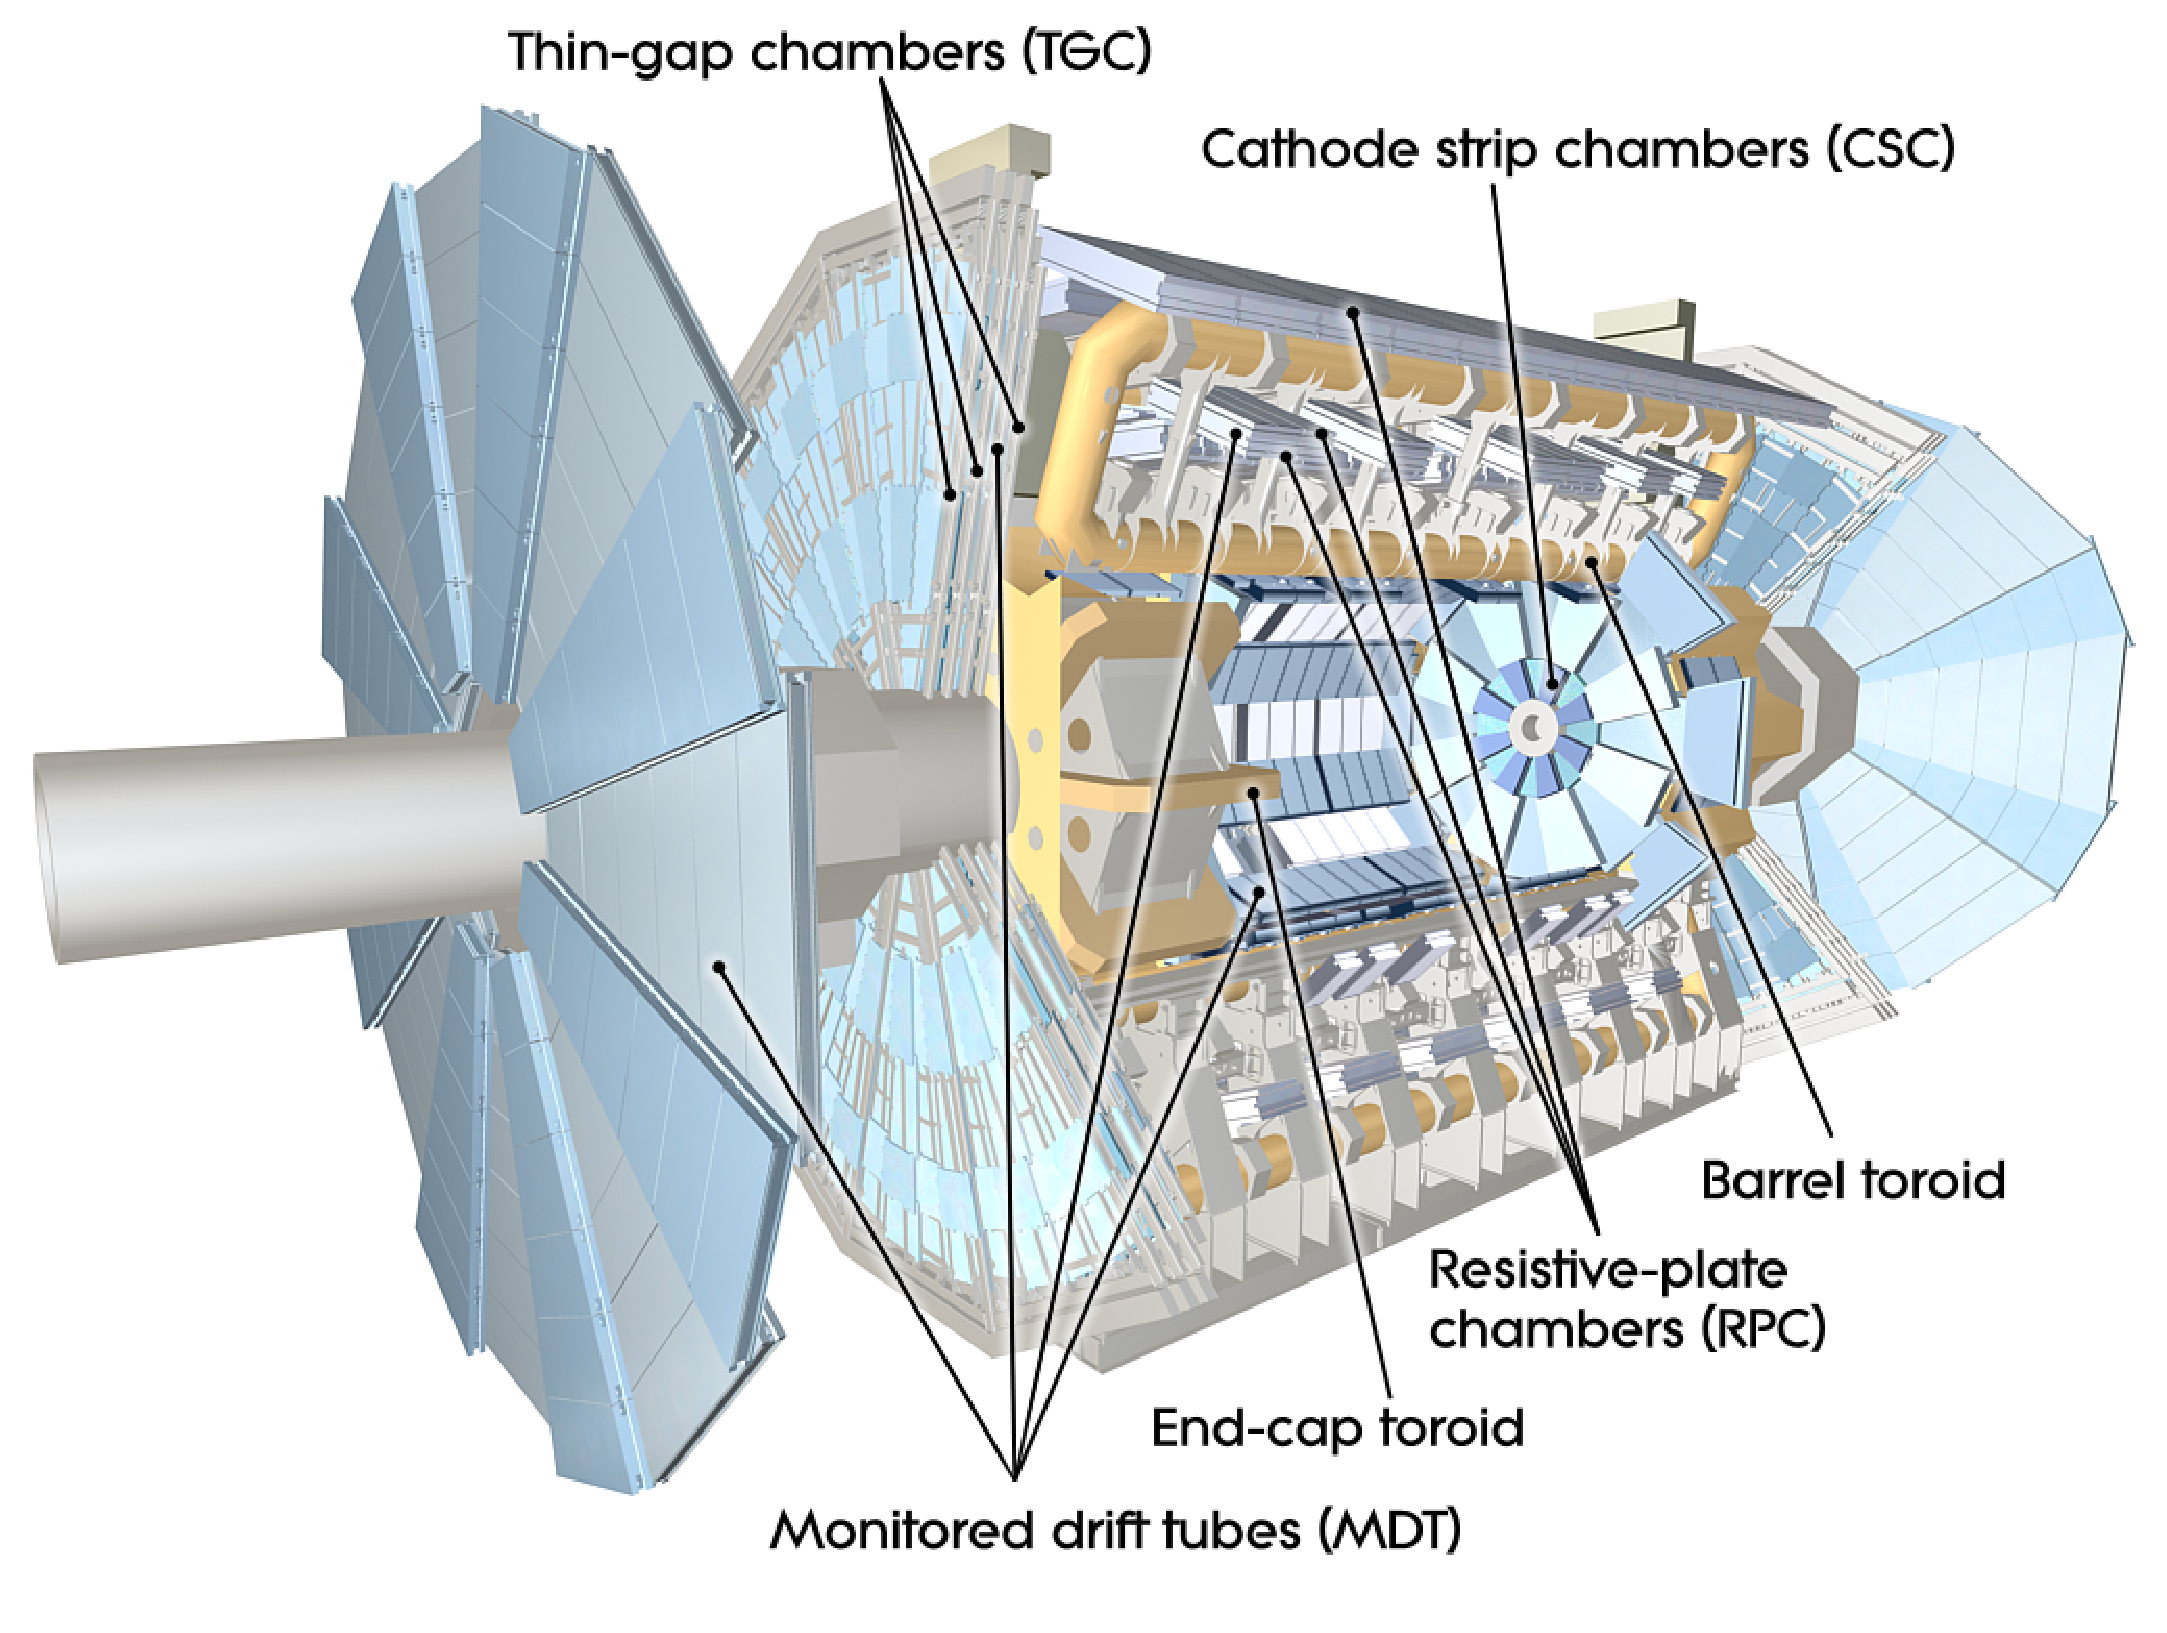
\includegraphics[width=0.7\textwidth]{ATLASdetector/Figures/MuonSystem.eps}
  \end{center}
  \caption{Schematic view of the ATLAS muon spectrometer.}
  \label{fig:MuonSpectrometerSchema}
\end{figure}

\subsubsection{Detection chambers}

\begin{description}
  \item[MDT] (Monitored Drift Tube chambers): 
    MDTs are proportional chambers based on pressurized drift tubes filled with an argon and carbon dioxide mixture and with a tungsten-rhenium wire producing a radial electric field.
%    made of aluminium with a diameter of \unit[30]{mm} and length varying from \unit[0.9]{m} to \unit[6.2]{m}.
%The gas mixture in them is 93\% Ar and 7\% $\text{CO}_2$, the anode is a $\unit[50]{\mu m}$ tungsten-rhenium wire producing a radial electric field.
Each chamber is composed of a group of six or eight tubes placed transverse to the beam axis.
This number of tubes allows for a very good track reconstruction and high reduction of the fake tracks from random associations of background hits, providing a resolution on position of $\unit[80]{\mu m}$ for an individual tube, $\unit[40]{\mu m}$ for a chamber and $\unit[30]{\mu m}$ for the three layers of MDTs.
    Due to their reliability, mechanical robustness and simpler operation, MDT chambers are employed to cover the larger area of the spectrometer ($\abseta <2.7$, $2.0$ for the innermost layer).
%The basic detection element is a cylindrical aluminum drift tube filled with gas and a central wire at a high potential.
%The muons passing through the tubes ionize the gas and produce charges that are collected on the wire.

  \item[CSC] (Cathode Strip Chambers): CSCs are multiwire proportional chambers with wires oriented in the radial direction, spaced by \unit[2.5]{mm}, and using the same gas mixture as the MDTs.
%The cathode strips are oriented, one perpendicularly to the anode wires (and gives the precision coordinate), and the other parallel to the wires (and gives the transverse coordinate).
  CSCs are used at high pseudo-rapidities to help confront the demanding rate and background conditions.
%They are arranged in a system of two disks with eight chambers each.
%Each chamber contains four multiwire proportional chambers (the CSCs)
%    The spatial resolution provided by one individual chamber is $\sim \unit[60]{\mu m}$.
    The spacial resolution of the four layers of CSCs is $\unit[40]{\mu m}$ in the bending plane and $\unit[5]{mm}$ in the non-bending one.
    The maximum drift time for signal collection is \unit[40]{ns} compared to the \unit[700]{ns} of the MDTs, which gives the possibility to achieve higher acquisition rates.
Due to this capability, together with the high radiation resistance, CSCs are used in the range $2.0 < \abseta < 2.7$.
\end{description}

\subsubsection{Triggering chambers}

For trigger purposes detectors with faster response than drift tubes are needed,\footnote{Drift-time in tubes with a diameter of $\sim \unit[10]{mm}$ can be of $\sim \unit[500]{ns}$, too long with respect to the \unit[25]{ns} spacing of the bunch crossings.}
MDTs and CSCs are therefore supplemented with special layers of trigger chambers.

\begin{description}
  \item[RPC] (Resistive Plate Chambers): RPCs are chambers with a gas mixture of $\text{C}_2\text{H}_2\text{F}_4$ (94.7\%), Iso-$\text{C}_4\text{H}_{10}$ (5\%) and $\text{SF}_6$ (0.3\%) between two resistive Bakelite plates.
    %separated by \unit[2]{mm} and containing a .
The avalanches are collected with two orthogonal sets of pick-up strips that provides a position resolution of \unit[1]{cm} in each plane and \unit[1]{ns} time resolution, allowing for individual bunch crossing discrimination.
RPCs provide also the $\phi$ coordinate for the tracks in the final analysis, since MDTs only give the $\eta$ coordinate.

  \item[TGC] (Thin Gap Chamber): TGCs are multi-wire proportional chambers with the characteristic that the wire-to-cathode distance is smaller than the wire-to-wire distance for a fast collecting time.
They are assembled in the end-cap wheels, covering the region $1.05 < \abseta < 2.7$ (2.4 for triggering).
The timing resolution is comparable to the RPC's one while the spatial resolution is in the range of \unit[2-7]{mm} for both coordinates.
\end{description}


\section{Forward subdetectors and luminosity measurement}
    \label{sec:LuminosityMeasurement}
    
A good determination of the integrated luminosity is of particular importance to reach the ultimate precision in measurement of processes of interest.
The luminosity, $\InstLumi$, defined in equation~\ref{eq:InstLumiDefinition}, can be rewritten as:
\begin{equation}
  \InstLumi = \frac{\mu_{\mathrm{vis}}n_b f_r}{\sigma_{\mathrm{vis}}}~,
\end{equation}
where $f_r$ is the collider revolution frequency, $n_b$ the number of colliding bunches
and $\sigma_{\mathrm{vis}}$ the visible inelastic \xsec\ (total inelastic \xsec\ times the detector acceptance and efficiency).
The  visible interaction rate per bunch crossing is denoted as $\mu_{\mathrm{vis}}$.
It is extracted mainly from the signals coming from specific luminosity detectors.
The simplest algorithm consists in ``simple counting'' of bunch crossings where detectors reported a signal, but more refined algorithms~\cite{Aad:2013ucp} are used,
in particular when the \pileup\ contamination is no longer negligible.

In order to use the measured $\mu_{\mathrm{vis}}$ for luminosity determination, 
each detector and algorithm must be calibrated by determining its
visible \xsec\ $\sigma_{\mathrm{vis}}$.
The calibration technique exploits the \textit{van der Meer}
scans~\cite{vdMscan}.
These are special low-intensity LHC 
runs where the beam separation in the transverse planes  is varied (scanned) in order to determine 
the beams' overlap profile.
Through the determination of the beam lateral profile the absolute luminosity of the particular run can be inferred using formula~\ref{eq:InstLumiDefinition}, and $\sigma_{\mathrm{vis}}$ can be determined for each subdetector.

    ATLAS is supplemented with several detectors in the forward regions to perform luminosity measurements and monitoring.
The main detectors for luminosity measurement are listed below:
\begin{description} 
%  \item[MBTS] (Minimum Bias Trigger Scintillators): located at $z = \pm \unit[365]{cm}$ from the interaction point, they cover the pseudorapidity region {$2.09<\abseta < 3.84$}.
%The MBTS were employed during 2010 to trigger on events with minimal requirement on collision activity.
%During 2011 and 2012, they were not considered as luminosity detectors given the saturation effect produced by the high interaction rate.
\item[LUCID] (LUminosity measurements using Cherenkov Integrating Detector): a Cherenkov detector specifically designed for luminosity measurement.
It consists of 16 aluminum tubes surrounding the beam pipe at \unit[17]{m} from the interaction point.
Each tube is filled with 
$\mathrm{C}_4\mathrm{F}_{10}$ and is coupled to a photomultiplier in the back-end.
\item[BCM] (Beam Conditions Monitor): $\unit[1]{cm^2}$ diamond detectors located at $z = \pm\unit[184]{cm}$ around the beam pipe.
  Their fast readout and good time resolution (\unit[0.7]{ps}) allow them to provide luminosity information for each bunch crossing.
At the same time they are also employed to trigger on beam losses and induce the dump of the beam, thus protecting the silicon detectors from damage that might result from an uncontrolled beam.

\item[ALFA] (Absolute Luminosity For ATLAS): is a subdetector that is only activated during special runs.
It consists of  8 scintillating fibers detectors placed at \unit[240]{m} from the interaction point inside roman pots, above and below the beam pipe.
\end{description}

In addition, cross-checks of the luminosity measurement have been performed using information from other standard subdetectors:
counting of primary vertices reconstructed by the ID and integrated signals from the Tile and forward calorimeter.
The precision achieved is of a few \% depending on the data-taking year.
\section{Trigger system}
    \label{sec:TriggerSystem}

    Due to technical limitations, not every LHC collision can be recorded by the ATLAS detector.
    The goal of the ATLAS trigger and data acquisition system is to select in real time events with interesting characteristics for physics analyses.
%The purpose of the trigger system is to reduce the input rate from several MHz to about $\unit[400]{Hz}$ for recording and offline processing.
%This limit is equivalent to an average data rate of about $\unit[300]{MB/s}$, which is the maximum that the computer resources and the offline storage can handle.
%For each bunch crossing, the trigger system verifies if at least one of hundreds of conditions (triggers) are satisfied.
%Most of them are based on identifying combinations of candidate physics objects such as electrons, muons or jets, but there are also triggers for inelastic $\pp$ collisions (minimum bias) and triggers based on global event properties, such as $\sum\et$ or $\met$.

\begin{figure}[!tb]
  \begin{center}
      \includegraphics[width=0.55\textwidth]{ATLASdetector/Figures/TriggerSystem.eps}
  \end{center}
  \caption[Schema of the ATLAS trigger system.]{Schema of the ATLAS trigger system.}
  \label{fig:TriggerSchema}
\end{figure}

The ATLAS trigger system~\cite{Aad:2012xs}, shown schematically in figure~\ref{fig:TriggerSchema}, has a three-layer structure with increasingly detailed levels of information used in the reconstruction, and hence refinement of the selection criteria at each stage.

% \subsection{Level 1 trigger}
% \label{L1}

At the first stage, Level 1 (L1), hardware triggers use coarse calorimeter and muon information for the trigger decision.
At this level the event rate is reduced from \unit[40]{MHz} (the frequency of the beam crossing) to a maximum of \unit[75]{kHz}.
In the cases where the trigger is passed, the L1 trigger defines one or more regions-of-interest (RoIs) in $\eta$ and $\phi$ where the trigger has identified interesting features. The raw event data is then sent to the readout stream for the next trigger level.

The Level 2 (L2) trigger is based on software.
At this stage the information from the trackers is incorporated to the RoI to build candidate objects (electrons, photons, muons) and their position and energy are computed. A tighter selection on these refined objects allows for a reduction of the throughput down to $\approx \unit[3]{kHz}$.

The final trigger level is the Event Filter (EF).
The combination of the two software steps, L2 and EF, is referred to as High Level Trigger (HLT).
At this point the physics objects are built using the same algorithms as the offline reconstruction. After the selection, the EF reduces the output rate to \unit[200]{Hz} and the events are written to mass storage.
Events passing the EF are assigned to streams defined to separate the events into different datasets for different analysis' interests, e.g. electron streams, muon streams, jet streams, etc.

Most of the trigger chains used for physics are un-scaled, meaning that all the events passing the selection are kept. 
Other trigger chains that contain either too many events
or events considered not physically interesting are pre-scaled. 
These are characterized by a prescaling value, $P$, meaning that of all the events that activated
the trigger, only $1/P$ were accepted.
These trigger chains are usually used for checks or calibration rather than physics analysis.

The term ``trigger chain'' refers to the sequence of selections
that define a certain trigger object. The naming convention is:
\begin{equation*}\label{eq:}
  {\rm [LEVEL][N][TYPE(S)][THRESHOLD][ISOLATION][QUALITY]},
  \end{equation*}
  where the components, from left to right, are: the trigger level used, the
  multiplicity of the type, the object candidate, the threshold applied to
  the transverse momentum or energy of the object candidate, the object isolation and
  the severity of the final algorithm requirements.

  Trigger chains define a {\it trigger menu}, where they are associated to their
  prescale value $P$, and which is chosen based on the physics program of the
  data-taking period, taking into account the LHC luminosity.

%During the course of 2011 the RoI-seeded approach at the EF was replaced by a full-scan strategy.
%It was found that sufficient time was available to read the information from the entire ATLAS calorimetry system, which improves the online selection efficiency.

\section{Data quality}
\label{sec:DataQuality}
Not all collision events recorded by ATLAS are used for data analysis.
Each subdetector maintains a record of its performance across the run, and only the data collected with the subdetectors meeting certain quality requirements are considered for the analysis.
Therefore, for each dataset Good Runs Lists (GRL) are compiled recording for each lumiblock\footnote{
A luminosity block (lumiblock) is the smallest unit of time in the ATLAS data-taking defined as the minimal period where all the data-taking configurations are constant. In general the duration of a luminosity block is of the order of 1 minute.} 
which subdetectors satisfied the requirements.
For the measurements presented in this dissertation, all ATLAS subsystems are needed, as the physics objects used in the analyses are reconstructed using the information from the full detector.
The fraction of data considered as ``good'' is $\sim 95\%$, giving a total integrated luminosity of $\unit[20.3]{fb^{-1}}$ satisfying data quality that is used for these analyses.

  \cleardoublepage
  \chapter{Event simulation}
\label{chapter:MCsimulation}

The precise comparison of observed data with the theoretical predictions is necessary to quantify the consistency with the SM or some of its possible extensions. The simulation of the physics processes and the interaction of particles with the detector is therefore needed to model the expected contributions from different background or signal sources. Computer programs known as Monte Carlo (MC) event generators are able to simulate events from defined physics processes. Pseudo-random numbers are used to simulate individual events reproducing on average the predicted distributions. Finally MC techniques are also used to simulate the interaction of particles with the detector materials and the read-out of the detector.

This chapter presents an overview of the simulation of \pp\ collisions, followed by a description of the MC generators used for the analyses in this dissertation and the ATLAS detector simulation.

\section{Simulation of \pp\ collisions}
\label{sec:pp_simulation}
The simulation of \pp\ collisions requires the description of physics processes involving very different energy scales. From the high-energy scales present in the deep-inelastic scattering between the partons in the protons, to the very low-energy scales of the final state when the partons evolve into stable hadrons. In this soft regime the physics involved can not be described by perturbative QCD, making a full analytic description of the process impossible.
%The simulation of proton collisions has an additional difficulty, since protons are not elementary particles. At high energies though, the partons inside the proton behave as asymptotically free, and the hard interaction can be described as a parton-parton collision.

Fortunately, a key aspect in the simulation of \pp\ collisions is the possibility of factorizing the different energy scales involved in the process. The simulation of the hard interaction can be computed up to a fixed order in perturbation theory, while the description of the softer scales can be done with phenomenological models.

The simulation of the full \pp\ collision can be therefore factorized into different steps. 
First, the modeling of the partons inside the proton can be separated from the actual interaction. Two of these partons can then collide and undergo an interaction with a large momentum transfer.
Given the high-energy scale of the interaction, it can be computed at fixed order in perturbation theory.
Since the partons involved in the collision are color charged they will emit gluons, which in turn radiate further gluons or split into quark/anti-quark pairs, leading to the formation of parton showers.
The radiation process continues until the partons reach an energy scale of $Q \approx \unit[1]{\gev}$. At this stage hadronization takes place, and partons recombine into colorless hadrons. Phenomenological models are used to describe the hadronization process as well as the decay of hadrons into the final state particles that interact with the detector.
The different steps involved in the simulation are illustrated in figure~\ref{fig:MCexample}.

\begin{figure}[!t]
  \centering
  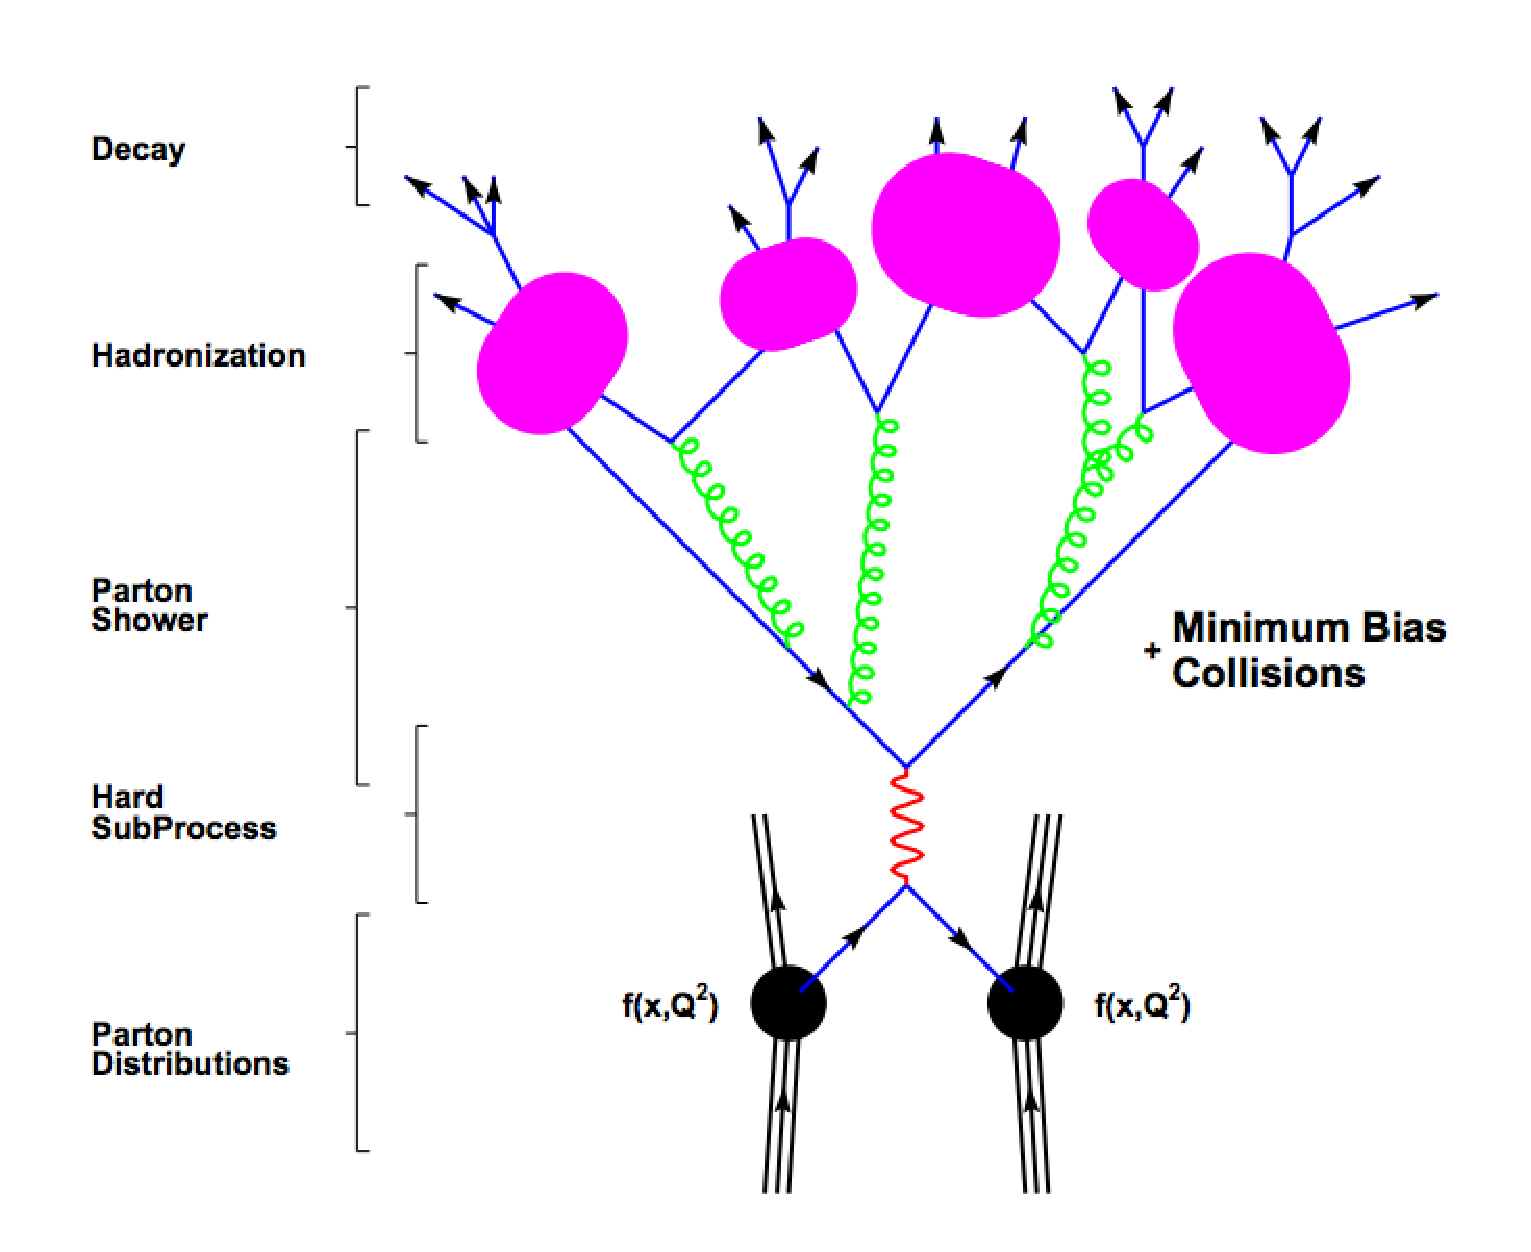
\includegraphics[width=0.7\textwidth]{MCsimulation/Figures/MCexample.eps}
  \caption{Representation of the different steps involved in the simulation of a \pp\ collision.}
  \label{fig:MCexample}
\end{figure}

\subsection{Factorization theorem}
The \xsec\ for a hadron collision producing a final state $X$, illustrated in figure~\ref{fig:hardscatter}, can be factorized into short- and long-distance effects delimited by a factorization scale, $\mu_F$, according to the factorization theorem~\cite{Collins:1989gx}:
\begin{equation}
  \sigma_{\pp \rightarrow X} = \sum_{a,b} \int dx_a dx_b\ f_a\left(x_a,\mu_F^2\right) f_b\left(x_b,\mu_F^2\right) \ \hat{\sigma}_{ab \rightarrow X}\left(x_a p_a,x_b p_b,\mu_F^2,\mu_R^2\right)~,
  \label{eq:factorization_theorem}
\end{equation}
where the sum runs over the parton types that can initiate the process.
%where $x_{i}$ is the fraction of momentum carried by the colliding parton  within the proton $p_{i}$, $f_{i}$ are the PDFs of each interacting parton, the sum runs over all parton types, and $\hat{\sigma}_{ab \rightarrow X}$ is the parton \xsec\ for incoming partons with momenta $p_{i} = x_{i} p_{i}$
The parton density function (PDF), $f_{i}\left(x_{i},\mu_F^2\right)$, encodes the probability of finding a parton of type $i$ within the proton, carrying a fraction of the proton's momentum $x_{i}$. 
PDFs are universal since they don't depend on the particular process. They are usually measured combining information from deep-inelastic scattering experiments and hadron colliders.

The \xsec\ for the partonic process $\hat{\sigma}_{ab \rightarrow X}\left(x_a p_a,x_b p_b,\mu_F^2,\mu_R^2\right)$ is computed explicitly at a fixed order in perturbation theory, which introduces a dependence on a renormalization scale $\mu_R$, that is usually chosen to be equal to $\mu_F$.
This step is also referred to as Matrix Element (ME) calculation, because it involves the calculation of the scattering matrix relating the initial and final state particles of the process.

\begin{figure}[!h]
  \begin{center}

    \myskip\begin{fmffile}{fmfhardscatter}
\unitlength=1mm
  \begin{center}
  \begin{fmfgraph*}(80,45)
    \fmfleft{P1,P2} \fmfright{P11,vv,P22}
    \fmf{fermion,tension=1,lab=$p_b$}{P1,g1}
    \fmf{fermion,tension=1,lab=$p_a$}{P2,g2}
    \fmfblob{.08w}{g1}
    \fmfblob{.08w}{g2}
    \fmf{plain,lab.side=left,lab=$x_bp_b$}{g1,v}
    \fmf{plain,lab.side=left,lab=$x_ap_a$}{v,g2}
    \fmf{dashes}{v,vv}
    \fmf{fermion}{g1,P11}
    \fmf{fermion}{g2,P22}
    \fmfv{lab.dist=.02w,lab=p}{P1}
    \fmfv{lab.dist=.02w,lab=p}{P2}
    \fmfv{lab.dist=.06w,lab.side=left,lab=$f_b(x_b)$}{g1}
    \fmfv{lab.dist=.06w,lab.side=left,lab=$f_a(x_a)$}{g2}
    \fmfv{decor.shape=circle,decor.filled=empty, decor.size=0.20w,lab.side=left,lab.dist=-0.35w,lab=$\hat{\sigma}(x_a,,x_b,,s)$}{v}
    \fmfv{lab=X}{vv}
    \fmffreeze
    \renewcommand{\P}[3]{\fmfi{plain}{%
        vpath(__#1,__#2) shifted (thick*(#3))}}
    \P{P1}{g1}{0,1}  \P{P1}{g1}{0,-1}
    \P{P2}{g2}{0,1}  \P{P2}{g2}{0,-1}
    \P{g1}{P11}{0,1} \P{g1}{P11}{0,-1}
    \P{g2}{P22}{0,1} \P{g2}{P22}{0,-1}
  \end{fmfgraph*}
  \end{center}
\end{fmffile}
\myskip
            %\myskip\input{fmfhardscatter}\myskip
%                \includegraphics[width=0.5\textwidth]{MCsimulation/Figures/hardscatter.png}
    \caption{Diagram of a generic hard scattering process. The partons, extracted from the colliding pp pair,
      carry a momentum fraction with respect to the proton energy described by a parton distribution function.
    The scattering of the partons is computed perturbatively and hence the kinematic properties of the final state object $X$ are predicted. }
    \label{fig:hardscatter}
  \end{center}
\end{figure}


\subsection{Fixed order QCD: matrix elements}
Schematically, the all-orders \xsec\ for the production of $X + \mathrm{anything}$, (inclusive $X$ production, with $X$ an arbitrary final state) can be expressed in the following way:
\begin{equation}
\hat{\sigma}_{ab\rightarrow X} \sim \underbrace{\sum_{k=0}^{\infty}{\int{d\Phi_{X+k}}}}_{\Sigma\text{ legs}}
                                          |\underbrace{\sum_{\ell=0}^{\infty}{\mathcal{M}^{\ell}_{X+k}} }_{\Sigma \text{ loops}}|^2~,
\label{eq:AllOrdersXSection}
\end{equation}
where the sum over $k$ represents the sum over additional ``real emission'' corrections (legs), and the sum over $\ell$ represents the sum over additional virtual corrections (loops).
$\Phi_{X+k}$ represents the phase space of the configuration with $k$ legs.

The various fixed-order truncations of a perturbative QCD calculation can be recovered by limiting the nested sums in equation~\ref{eq:AllOrdersXSection} to include only specific values of $k+\ell$:

\begin{itemize}
\item $k=0$, $\ell=0$: Leading order for inclusive $X$ production.
\item $k=n$, $\ell=0$: Leading order for $X+n$~jets.
\item $k+\ell \leq n$: N$^n$LO for $X$ (includes N$^{n-1}$LO for $X+1$ jet,  N$^{n-2}$LO for $X+2$ jets, and so on up to LO for $X+n$ jets).
\end{itemize}

Figure~\ref{fig:tt_jets} shows an example of several Feynman diagrams for a \ttbar\ final state at tree level ($k=0$, $\ell=0$), first emission ($k=1$, $\ell=0$) and including a virtual correction ($k=0$, $\ell=1$).
\begin{figure}[t!]
  \centering
  \begin{subfigure}{0.32\textwidth}
  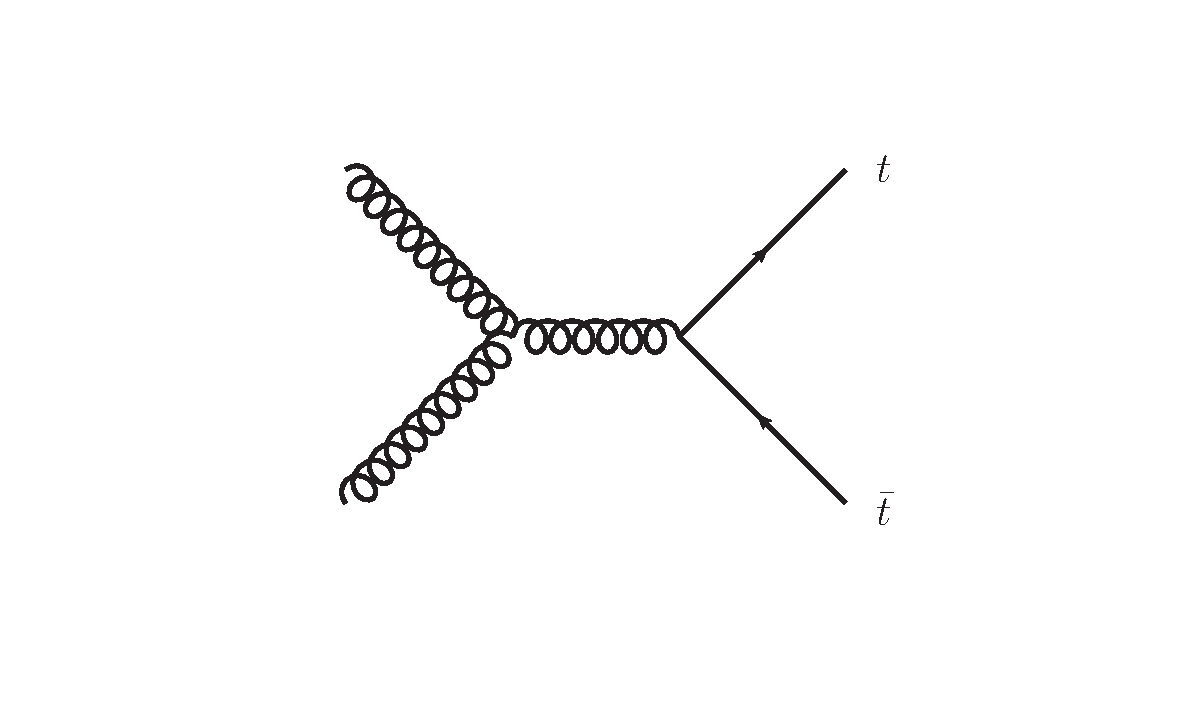
\includegraphics[width=\textwidth]{MCsimulation/Figures/tt_0jet}
  \caption{}\end{subfigure}
  \begin{subfigure}{0.32\textwidth}
  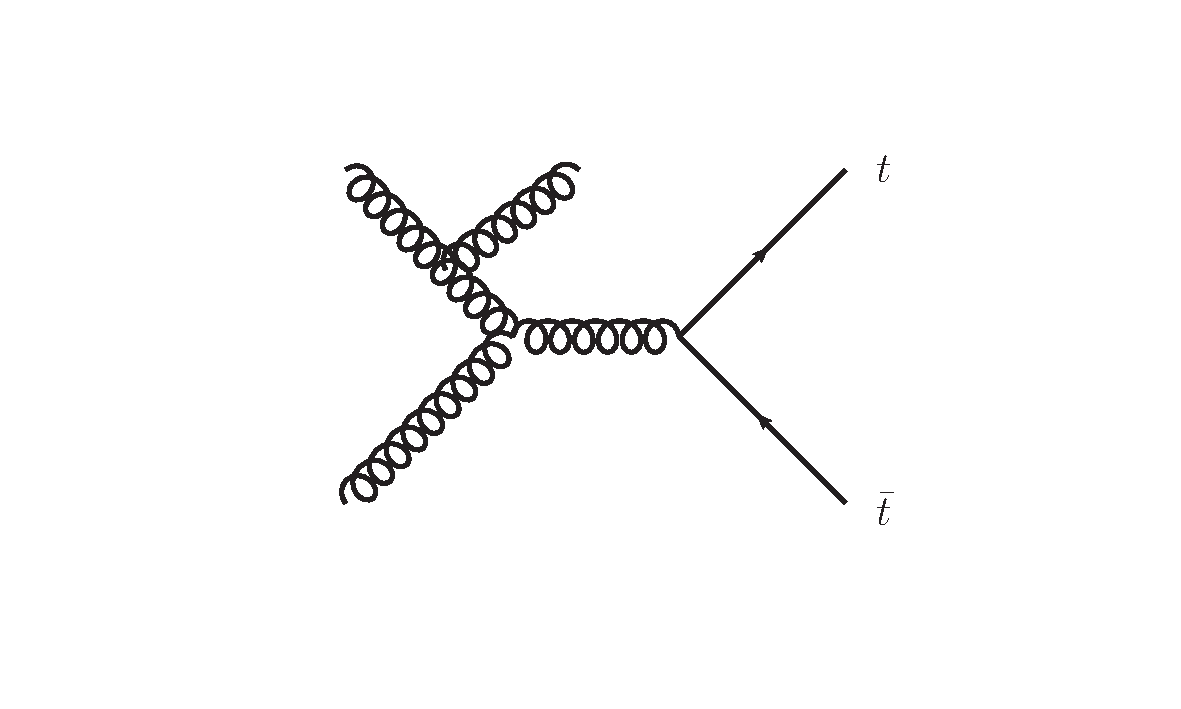
\includegraphics[width=\textwidth]{MCsimulation/Figures/tt_1jet}
  \caption{}\end{subfigure}
  \begin{subfigure}{0.32\textwidth}
  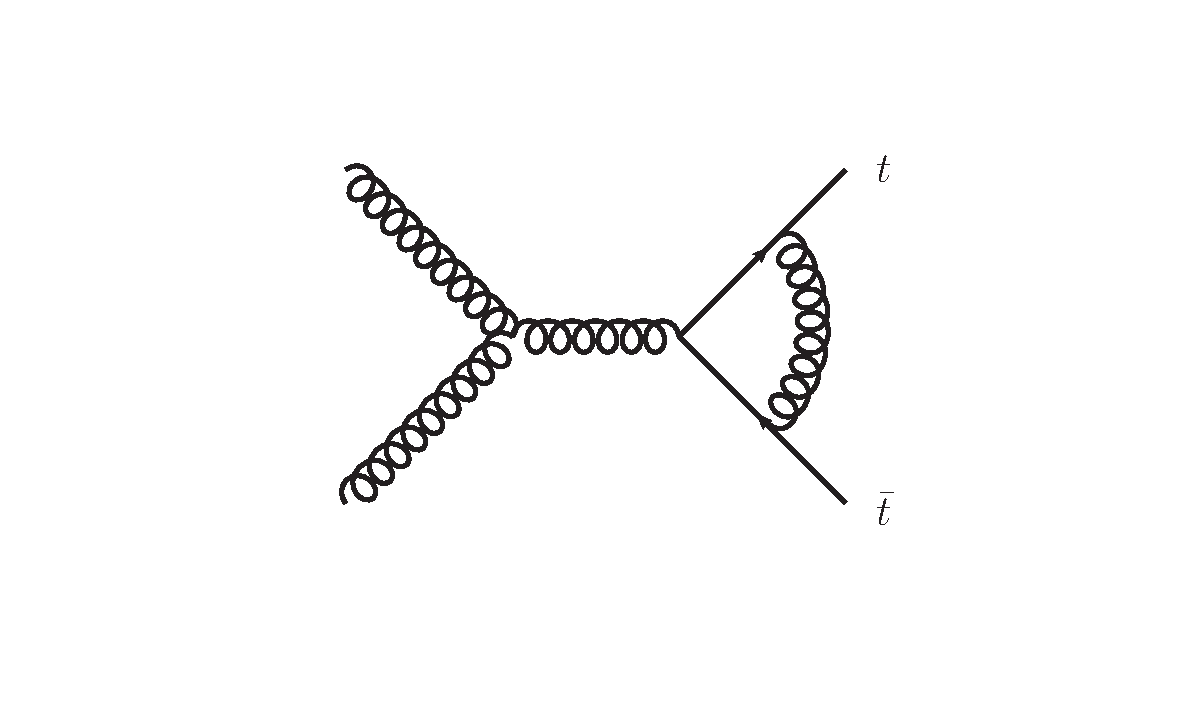
\includegraphics[width=\textwidth]{MCsimulation/Figures/tt_1loop}
  \caption{}\end{subfigure}
  \caption{Example Feynman diagrams of \ttbar\ production for (a) leading order, (b) first real emission and (c) first virtual correction.}
  \label{fig:tt_jets}
\end{figure}

The KLN theorem~\cite{KLN1,KLN2} states that the divergences originated in the loops exactly cancel against those from the real emissions, order by order in perturbation theory.
However, in a fixed-order calculation, e.g. leading order, in the situation for which $k\geq1$, $\ell=0$, the integration over the full momentum phase space will include configurations in which one or more of the $k$ partons become collinear or soft, thus leading to singularities in the integration region.
For this reason, the integration region needs to be modified to include only ``hard, well-separated'' momenta.
The remaining part of the phase space is then considered by the parton shower generators.

\subsection{Parton Shower}

Parton showers are included in the MC simulations to approximately account for the rest of higher order contributions to emulate a complete final state.
A parton shower generator simulates the successive emission of quarks and gluons from the partons in the final (or initial) state.
This simulation is approximate, since it assumes completely independent parton emissions and does not consider virtual corrections.
In the almost-collinear splitting of a parton, the $n+1$-parton differential \xsec\ can be related to the $n$-parton \xsec\ before splitting as:
\begin{equation}
  d\sigma_{n+1} \approx d\sigma_n~dP_i(z,q^2) \approx d\sigma_n~\frac{\alpha_S}{2\pi}\frac{dq^2}{q^2}dz~P_{ji}(z)~,
  \label{eq:splitting}
\end{equation}
where $dP_i(z,q^2)$ is the probability that parton $i$ will split into two partons at a virtuality scale or invariant mass $q^2$, with parton $j$ carrying a fraction $z$ of the momentum of parton $i$. An illustration of this process is given in figure~\ref{fig:splitting}.
\begin{figure}[t!]
  \centering
  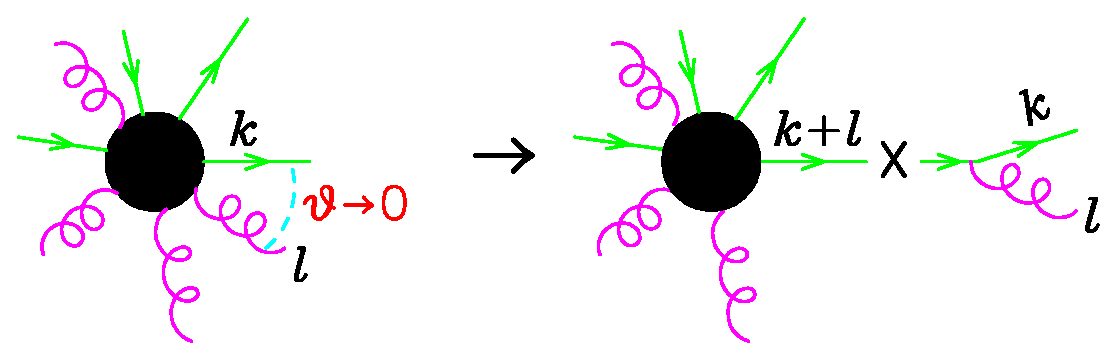
\includegraphics[width=0.7\textwidth]{MCsimulation/Figures/factorization}
  \caption{Representation of an $n+1$-parton process described as a splitting from an $n$-parton process.}
  \label{fig:splitting}
\end{figure}
%and $\phi$ are the opening angle and azimuthal angle of the splitting, and $P_i$ is the splitting function, which describes the distribution of the fraction $z$ of energy of the original parton, assigned to the new parton. 
There are three possible processes for QCD emission (splitting): $q \rightarrow gq$, $g \rightarrow gg$ and $g \rightarrow \qqbar$.
The simulation algorithm develops the shower by applying equation~\ref{eq:splitting} iteratively, for each parton involved in the hard interaction.

The implementation of the parton shower in MC programs is done via the Sudakov form factors:
\begin{equation}
  \Delta_i(q_1^2,q_2^2) = \text{exp} \left( - \sum_j \int_{q_2^2}^{q_1^2} \int_{z_{\text{min}}}^{z_{\text{max}}}  dP_i(z,q^2) \right)~.
  \label{eq:sudakov}
\end{equation}
The Sudakov form factors represent the probability that a parton evolves from an initial scale $q_1$ to a lower scale $q_2$ without splitting.

In final-state showers, the branching algorithm operates in the following steps:
\begin{enumerate}
  \item Given the initial scale $Q^2$, partons emit radiation at a scale $q_2$ determined by sampling equation~\ref{eq:sudakov}.
\item If the scale $q_2^2$ is below the hadronization scale, $q_2^2 < Q_0^2 \approx \unit[1]{\gev^2}$,  the shower development is terminated and hadronization takes place.
\item  Otherwise, the procedure is repeated for each new parton produced by the splitting, taking $q_2^2$ as initial scale.
\end{enumerate}

In the case of initial-state showers, the radiation is emitted by the colliding partons, and the final energy scale is the one entering the hard interaction. MC generators implement a \textit{backward evolution} that starts by setting the correct parton momentum for the hard scatter, and then develops the shower backwards, with ancestor partons gaining energy at each emission.

\subsection{Matrix element and parton shower matching}
The simplest fixed-order ME calculation is the LO one, $k=0$ and $l=0$ as represented in equation~\ref{eq:AllOrdersXSection}. However the precision of the pure LO calculation is often not sufficient for an accurate description of the final state. In this case multi-leg LO ($k \geq 1$, $l=0$) or N$^n$LO calculations ($k+l = n$) can be used, although with an infrared cut-off to prevent divergences from soft and collinear emissions. 
A problem arises when adding the parton shower evolution, since a double counting of certain phase space regions is present. A given final state with one additional emission is generated as both the ME term for $X+1$ parton, and in the first radiation of the parton shower starting from the $X+0$ parton state.

To remove this overlap, the phase space covered by the ME calculation, and the space covered by the parton-shower evolution needs to be separated. The procedure to distinguish between hard and large-angle emissions, described by the ME, and soft and collinear emissions, described by the PS, is referred to as ME-PS \textit{matching}.
The most widely-used matching schemes are the Catani-Krauss-Kuhn-Webber (CKKW \cite{Catani:2001cc}) and the Michelangelo L. Mangano (MLM \cite{Mangano:2006rw}) algorithms.

In the CKKW algorithm, a parton branching history is generated using the \kt algorithm \cite{Catani:1991hj}, given a configuration with $n$ partons in the final state.
The values of $\alpha_s$ in every vertex of the branching, and the Sudakov factor from every line between the vertices, are used to reweight the ME.
The initial conditions of the shower are then set to have a smooth transition between the reweighted ME and the parton shower, where the hard emissions in the shower evolution are vetoed if they have enough transverse momentum to produce a separate jet, according to the \kt algorithm.

The MLM algorithm starts by separating the events in exclusive samples of $n$ partons in the final state, on which the parton shower is added.
The parton configuration after the showering is then processed with a cone jet algorithm, with a radius $R_{\text{jet}}$.
The original $n$ partons are matched to the jets if $\Delta R(\text{jet}, \text{parton}) < R_{\text{jet}}$.
If all the partons are matched to a jet and there are no extra jets, i.e. $N_{\text{jets}}=n$, the event is accepted.
Otherwise, the event is rejected to avoid further hard emissions that would lead to additional jets.
Finally, the events with different jet multiplicities, $n=0, 1, 2, \ldots, k$, are recombined in a single sample.
The events in the sample with highest parton multiplicity $k$ are accepted if $N_\text{jets}\geq k$.

\subsection{Hadronization}
    \label{subsec:HadronizationModels}
As the partons evolve and radiate, the values of the shower evolution scale $Q^2$ decrease bringing the parton virtuality below the hadronization scale $Q_0^2 \approx \unit[1]{\gev}$. The confining effects of QCD become important and the dynamics enter a non-perturbative phase which leads to the formation of the observed final-state hadrons.
Event generators have to rely on phenomenological models based on general features of QCD.
The most used hadronization models are the string fragmentation and the cluster hadronization models, illustrated in figure~\ref{fig:HadronizationModels}.

In the string model~\cite{Andersson:1983ia,Sjostrand:1984ic}, the confinement between partons induced by the color force is represented by a gluonic string. For a quark-antiquark pair, as the color charges move apart, the string is stretched, and its potential energy grows. When the energy becomes of the order of hadron masses, it becomes energetically favorable for the string to break and create a new quark-antiquark pair. The two segments of string will stretch and break again, until all the energy has been converted into quark-antiquark pairs connected by short strings.

The cluster model~\cite{Webber:1983if,Marchesini:1987cf} relies on groupings of partons to form colorless clusters, after forcing the final state gluons to split into quark-antiquark pairs. The heaviest clusters can decay and split into smaller clusters. Most clusters will have masses below \unit[3]{\gev}, and their decay into hadrons is simulated with three-body models with intermediate resonances.

\begin{figure}[!t]
  \begin{center}
    \begin{subfigure}{0.3\textwidth}
        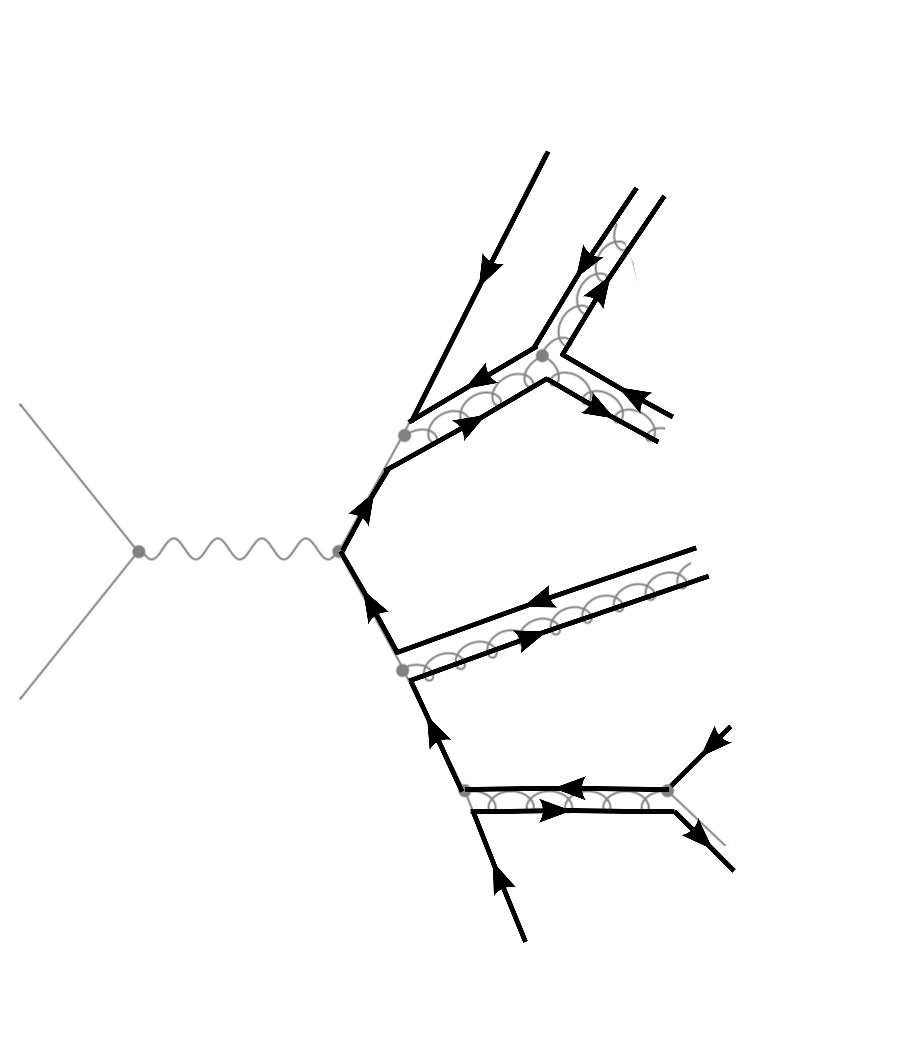
\includegraphics[width=\textwidth]{MCsimulation/Figures/had_colorflow.eps}
        \caption{}\end{subfigure}
    \begin{subfigure}{0.3\textwidth}
        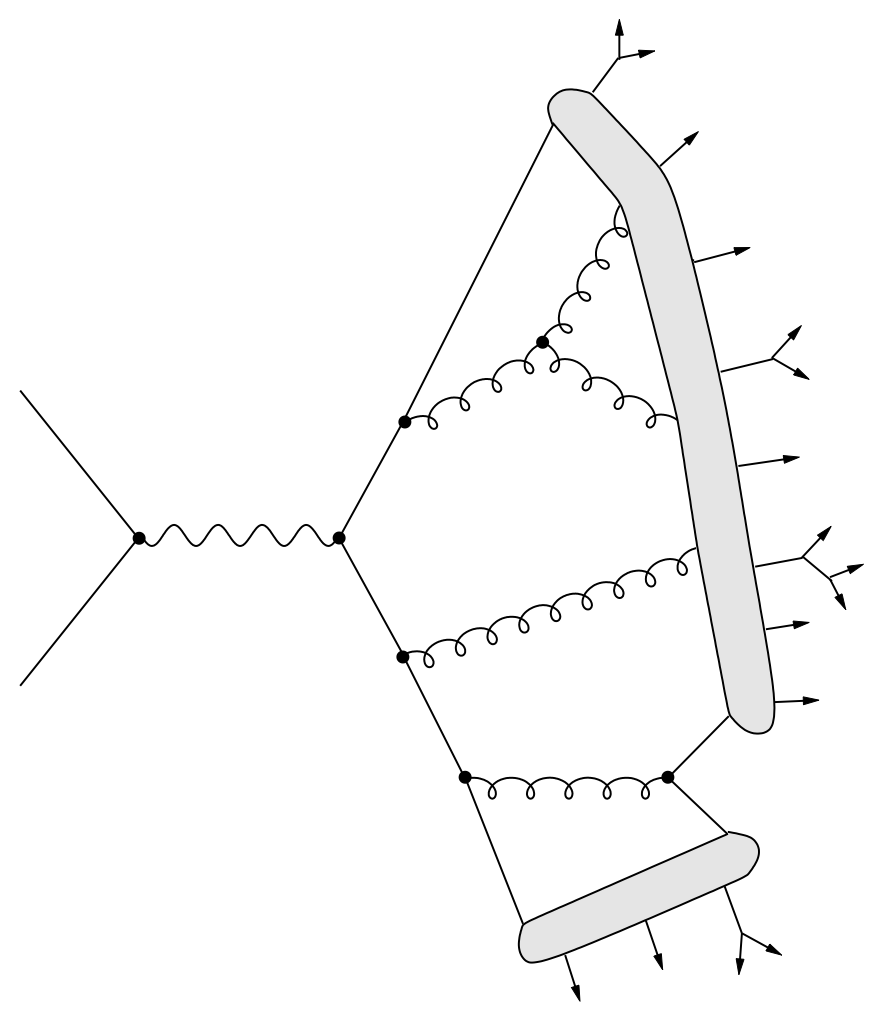
\includegraphics[width=\textwidth]{MCsimulation/Figures/HadronizationString.eps}
        \caption{}\end{subfigure}
    \begin{subfigure}{0.3\textwidth}
        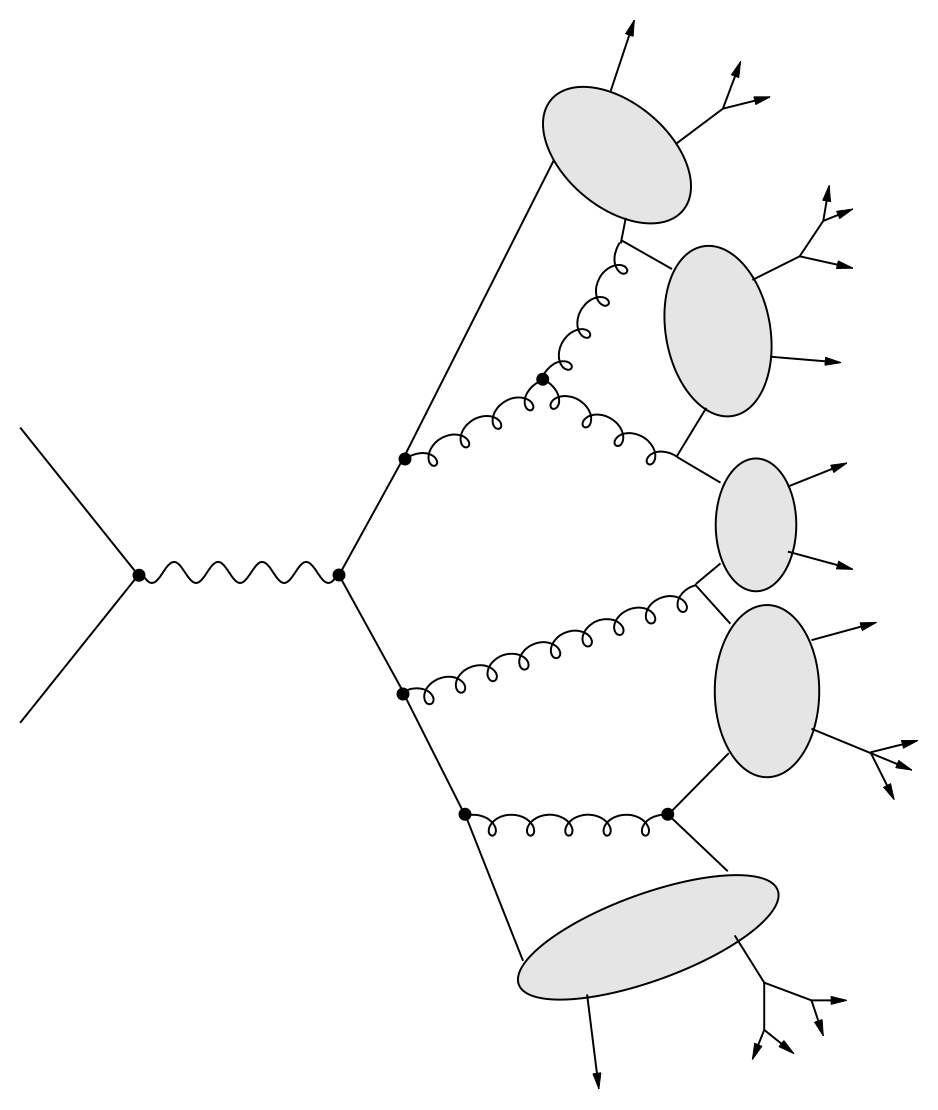
\includegraphics[width=\textwidth]{MCsimulation/Figures/HadronizationCluster.eps}
        \caption{}\end{subfigure}
  \end{center}
  \caption[Illustration of different hadronization models.]{Illustration of (a) the color flow in a given parton configuration and the models of (b) string fragmentation and (c) cluster hadronization.}
  \label{fig:HadronizationModels}
\end{figure}


\subsection{Underlying event}
The underlying event (UE) refers to the soft interactions involving spectator partons from the colliding protons. Because of the low energy scale of these processes, phenomenological models have to be used, where the parameters are tuned based on experimental data~\cite{Aad:2014hia}, such as the charged particle density (see figure~\ref{fig:UE}).
The large \xsec\ for gluon-gluon scattering makes multiple gluon scatterings per proton collision very likely. For this reason the generic soft scattering of partons is referred to as multiple parton interactions (MPI). The color connection with the beam remnants that are not interacting is also simulated with phenomenological models~\cite{Sjostrand:2006za,jimmy}.

\begin{figure}[!ht]
  \begin{center}
        \includegraphics[width=0.7\textwidth]{MCsimulation/Figures/figaux_04b}
  \end{center}
  \caption{Normalized charged-particle \pt\ sum density distributions in ATLAS data compared to different underlying event models. From reference~\cite{Aad:2014hia}.}
  \label{fig:UE}
\end{figure}
\subsection{\Pileup}
In-time \pileup\ events are originated from the scattering of protons in the same bunch of the hadron generating the hard process of interest. They mainly consist of soft QCD interactions and are modeled in a similar way as the UE. Out-of-time \pileup\ is modeled with the same physics process, but considering interactions in past bunch crossings and simulating the time response of the readout electronics.

\section{Monte Carlo generators}
\label{sec:MCgenerators}
Different Monte Carlo generators are used for the description of different physics processes of relevance. Generators can be classified as either multi-purpose generators, capable of performing the full simulation chain, or ME generators which have to be interfaced with an additional parton shower.

\subsection{General purpose Monte Carlo generators}
\begin{description}
  \item[\pythia~\cite{Sjostrand:2006za}] is a multi-purpose MC generator using LO calculations for $2 \rightarrow n$ ($n \leq 3$) processes and PS with emissions ordered in transverse momentum. The Lund string model is used for hadronization, and UE simulation is included.
  \item[\herwig~\cite{Corcella:2000bw}]  is a multi-purpose MC generator using LO calculations for $2 \rightarrow 2$ processes and PS with emissions ordered in opening angle. The cluster model is used for hadronization and for the UE description. \herwig\ is typically interfaced with the standalone software \jimmy~\cite{Butterworth:1996zw} that simulates UE and MPI.
\end{description}

\subsection{Multi-leg leading-order generators}
\begin{description}
\item[\alpgen~\cite{Mangano:2002ea}] is a MC generator providing LO calculations of $2 \rightarrow n$ ($n \leq 9$) processes. It can be interfaced with either \pythia\ or \herwig\ for parton shower evolution, hadronization and UE modeling. ME-PS matching is applied with the MLM algorithm.
\item[\madgraph~\cite{Alwall:2011uj}] is a MC generator specialized in the computation of ME involving $2 \rightarrow n$ ($n \leq 6$) processes at LO. It is interfaced with \pythia\ for the parton shower evolution and the ME-PS matching is performed with the MLM algorithm.
\item[\sherpa~\cite{Gleisberg:2008ta}] is a MC generator that can provide multi-leg leading-order calculations. It contains its own parton shower algorithm based on the Catani-Seymour dipole formalism~\cite{Schumann:2007mg}. The ME-PS matching is implemented with an improved version of the CKKW algorithm~\cite{Hoeche:2009rj}.
\end{description}

\subsection{NLO generators}
\begin{description}
  \item[\powheg~\cite{Frixione:2007vw}] is an event generator computing ME at NLO in perturbative QCD. \powheg\ can be interfaced with either \pythia\ or \herwig\ for the modeling of the parton shower, hadronization and UE. 
  \item[\sherpa] can also generate events at NLO after being interfaced with additional libraries to compute the loop amplitudes. \sherpa\ in conjunction with \OpenLoops~\cite{Cascioli:2011va} is used to model the \ttbb\ process at NLO, which is the largest background for the analyses discussed in this dissertation.
\end{description}

\section{ATLAS simulation}
\label{sec:ATLASsim}
The final output of the MC generators is a list of four-vectors of all stable particles produced in the event, after decay and hadronization of the intermediate unstable particles. This output can be used in order to study the physics processes at the \textit{particle level}. In order to compare it with the recorded data, the MC has to be analyzed after the reconstruction in the detector, i.e. at the \textit{reconstruction level}. The detector simulation software, \Geant~\cite{G4}, models the interaction of the particles with the detector. The simulation of the interaction converts the energy deposits into electronic signals taking into account the geometry, materials and readout system of the ATLAS detector.
A less refined simulation, known as Atlfast-II or AF2~\cite{AF2}, is also available. This reduces considerably the CPU time necessary to process the events by applying a parameterized description of the particle showers in the calorimeters.

Figure~\ref{fig:reco_flow} shows the ATLAS simulation data flow with the different steps of the MC and data processing.

\begin{figure}[hbt!]
  \begin{center}
  	\includegraphics[width=0.9\textwidth]{MCsimulation/Figures/outline_v3} %v2 without the color lines
	\caption{The flow of the ATLAS simulation software, from event generators (top left) through reconstruction (top right).
        The red path leads to {\it particle level} physics objects, the blue path to
        {\it reconstructed level} physics objects, while the green path shows the real data
        flow to physics objects.
        %Algorithms are placed in square-cornered boxes and persistent data objects are placed in rounded boxes. 
        %The optional pile-up portion of the chain, used only when events are overlaid, is dashed. 
        %Generators are used to produce data in HepMC format.  
        %Monte Carlo truth is saved in addition to energy depositions in the detector (hits). 
        SDO stands for Simulated Data Object, ROD for Read Out Driver~\cite{Aad:2010ah}.}
\label{fig:reco_flow}
\end{center}
\end{figure}

%The \Geant\ parameters are tuned using test-beam and \pp\ collision data. The accuracy of the detector simulation is based on the information from the geometry database, which contains the description of the detector volumes in terms of dimensions, geometry, position and material composition, while the conditions database provides the information on the detector real-time conditions like dead channels, misalignments, or temperatures. Since conditions vary from run to run, it is important that the detector simulation reproduces as close as possible the real status of ATLAS during a particular data-taking period. %rewrite
%

\section{Monte Carlo corrections}
\label{sec:mcweights}

Monte Carlo samples are corrected to reproduce the best known theoretical \xsec,
usually NLO or NNLO, even when they are produced with a lower order MC generator.
In addition to the normalization to the recorded luminosity, the events are weighted
to match the expected number of interactions per bunch crossing $\left<\mu\right>$
 in real data-taking conditions. 

To ensure an accurate modeling of the detector effects in the reconstruction and identification efficiencies $\varepsilon$, the efficiencies in MC are corrected with multiplicative scale factors. The scale factors are defined as:
\begin{equation}
  SF = \frac{\varepsilon_{\rm data}}{\varepsilon_{\rm MC}}
  \label{eq:SF}
\end{equation}
where $\varepsilon_{\rm data}$ and $\varepsilon_{\rm MC}$ are measured in dedicated data calibration samples and in the equivalent MC simulation, respectively. Analogously, energy scale and resolution of the different physics objects in the simulation are corrected to match the corresponding measurements in data.

  \cleardoublepage
  \chapter{Reconstruction of physics objects}
    \label{chapter:ReconstructionOfObjects}

This chapter describes the reconstruction of the main physics objects that are relevant for the analyses presented in this dissertation.
The identification, reconstruction and calibration of electrons, muons, jets, $b$-jets and missing transverse energy is discussed in detail.
A brief description of the systematic uncertainties associated with these physics objects is also included.

\section{Tracks}
%Rewrite, stolen from Francesco
In the solenoidal magnetic field of the ID,
a charged particle moves along a helicoidal trajectory with
a curvature inversely proportional to its momentum. 
Tracks are the reconstruction of these trajectories from the 
electric signals induced in the detectors.
Therefore, tracks are used to identify charged particles and 
measure their momenta. 
In addition, the extrapolation of the trajectories allows
the identification of the interaction vertices and the reconstruction of decays of long-lived particles such as $b$-hadrons.

Several pattern recognition algorithms~\cite{Cornelissen:1020106} are used to find tracks in the ID.
The tracks typically used in physics analyses are found using an \textit{inside-out} pattern recognition algorithm, which starts building track ``seeds'' considering space points in the silicon detectors and then extending the track candidate 
outwards to the TRT. An \textit{outside-in} sequence, also referred to as back-tracking, takes into account all the hits not considered by the previous algorithm. It is seeded in the TRT and the track candidate is then extrapolated to the silicon detectors.

A reconstructed track is fully specified by the following parameters:
\begin{equation}
( d_0 , z_0 , \phi , \theta , q/p) 
\end{equation}
where $d_0$ and $z_0$ represent the minimum distance to the center of the detector in the transverse plane and in the longitudinal direction respectively. The azimutal and the polar angle are denoted by $\phi$ and $\theta$ respectively, and $q/p$ represents the charge over momentum. Impact parameters and direction are often expressed with respect to the main primary vertex in the event.

\section{Primary vertices}
Due to the large number of protons per bunch crossing, multiple interaction vertices can be reconstructed in the event.
Primary vertices are reconstructed from the combination of reconstructed
tracks with an adaptive vertex fitting algorithm~\cite{ATLAS-CONF-2010-069}
and they are constrained to lie within the estimated position of the beam spot.\footnote{The beam spot is defined as the spatial region around the interaction point where the profiles of the two beams overlap.}

In order to improve the resolution on the vertex spatial position, only vertices that have at least five tracks with $\pT>500 \MeV$ associated with them are considered.
The number of reconstructed primary vertices is used as a measure of the in-time \pileup\ and several calibration parameters depend on it.

The vertex with the highest sum of the squared track $\pT$ is assumed to be the main vertex of the event corresponding to the hardest $\pp$ interaction. 
The rest of the primary vertices are considered \pileup\ interactions.
Vertices incompatible with the beam collision region are considered secondary vertices, also referred to as displaced vertices.
%They typically originate from decays of long-lived particles. 
The reconstruction of secondary vertices is useful to identify $b$- and $c$-hadrons, as it will be described in section~\ref{sec:btagging}.
%The kinematics of the physics objects
%are then recomputed considering this vertex as a new reference point.

\section{Leptons}
\label{sec:Leptons}
The reconstruction and identification of electrons and muons will be discussed.
Tau-lepton reconstruction is not considered since they will not explicitly be used in any of the analyses described in this dissertation.
Although no attempt is made to identify the tau-leptons, their decay products can still contribute to the object reconstruction.
Leptonic tau decays can be identified as isolated electrons or muons, whereas hadronic tau decays are reconstructed as narrow jets in the detector.

\subsection{Electrons}
    \label{subsec:Electrons}
    Electron candidates are built by searching for a narrow, localized cluster of energy in the EM calorimeter, with at least one ID track associated to it~\cite{Aad:2014fxa}. A sliding-window clustering algorithm~\cite{Lampl:2008zz} is used to identify electron clusters. The algorithm performs a scan of the calorimeter, searching for local maxima of energy within a window of dimensions $3 \times 5$ in units of $0.025\times0.025$ in $\Delta \eta \times \Delta \phi$ space.

Tracks from the inner detector are extrapolated to the middle layer of the electromagnetic calorimeter and matched to the cluster seed. The absolute value of $\Delta\eta$ between the cluster and the track, $|\Delta\eta|$, has to be smaller than $0.05$.  The $\Delta\phi$ must satisfy the relationship $ -0.05 < q\cdot\Delta\phi < 0.10 $. The sign-corrected $\Delta\phi$ selection takes into account the bending direction of the electron in the solenoidal magnetic field.
Matched clusters are then rebuilt with a slightly larger window, $3\times7$ or $5\times5$, depending on whether they are located in the barrel or in the end-cap.

The electron four-momentum is built from the cluster energy and the direction of the associated ID track.
The final cluster energy is obtained by correcting for the energy losses in the material in front of the calorimeter, the lateral leakage due to the fixed cluster size and the longitudinal leakage in the hadronic calorimeter.
Such corrections are derived from detailed studies in MC simulation, test beams and ${Z \rightarrow e^+e^-}$ data events~\cite{Aad:2014nim}.

Electron identification is performed on the candidate electrons in order to suppress the mis-identification of other particles. 
Different conditions on cluster shape are applied, using the fact that the shower development is narrower for electrons than for hadrons, and the hadronic leakage is smaller. 
Track-quality requirements reduce the impact of accidental track association with photons, energetic $\pi^0$ or $\rho$ mesons with electromagnetic decays that can be reconstructed as a single energy cluster. 

Three reference selections have been produced with increasing background rejection: \textit{loose}, \textit{medium} and \textit{tight}. 
Figure~\ref{fig:OBeleID} shows the comparison of the efficiency for each benchmark selection~\cite{EGAMMAsf}. The identification efficiencies depend on the electron $\et$ and pseudo–rapidity, while they are not strongly affected by \pileup. The efficiencies are measured using the ``tag-and-probe'' method.
This method selects a clean and unbiased sample of leptons (probe) from $Z$ boson
decays using selection cuts on one of the leptons in the decay
(tag). The efficiency is determined by applying the selection to the probe lepton.
The modeling in simulation differs slightly from what is observed in data, therefore a calibration scale factor is applied in MC samples.

\begin{figure}[tb!]
\centering
\begin{subfigure}[b]{0.49\textwidth}
\includegraphics[width=\textwidth]{Objects/Figures/Fig5a_electronid_et.eps}
\caption{}
\end{subfigure}
\begin{subfigure}[b]{0.49\textwidth}
\includegraphics[width=\textwidth]{Objects/Figures/Fig7a_electronid_npv.eps}
\caption{}
\end{subfigure}
\caption{ (a) Electron identification efficiency as a function on electron \ET\ for the benchmark selections in data and MC. 
(b) Measured electron identification efficiency in data for the different benchmark selection as a function of the number of reconstructed primary vertices in the event. 
}
\label{fig:OBeleID}
\end{figure} 

Finally, an additional isolation requirement can be applied to reject electrons from semi-leptonic decays of heavy hadrons. 
The track isolation variable $\pT^{R}$ is defined as the sum of the transverse momenta of all the tracks in a cone of radius $R$ around the electron direction. Only tracks with $\pT > 1 \GeV$ and compatible with being originated from the primary vertex are considered
with the exception of the track used to build the electron object. 
The calorimetric isolation variable called $\ET^{R}$ represents the sum of the transverse energy of the calorimetric cells in the cone of radius $R$ around the electron with the deposit associated with the electron itself subtracted.
%Additional corrections are applied to improve the performance of the calorimetric isolation~\cite{EGAMMAiso}. 
%Due to the fixed size of the electron cluster, higher-energy clusters tend not to be fully contained and, as a net effect, the isolation energy increases as a function of the electron \pT\ even for well isolated electrons. 
%A \pT-leakage correction is derived from MC to compensate for this effect.
%In order to compensate for the \pileup\ effect, an ambient energy density (ED-correction) subtraction is applied. This technique is very similar to the one used for the jet calibration and will be further discussed in the jet section.
The variables  $\ET^{0.2}$ and $\pT^{0.3}$ have been chosen, 
%This stems from the fact that, even after the \pileup\ suppression, smaller cone sizes are preferable due to the topology of \ttbar\ events where jets are likely to be found closer to the selected electrons. %%% \cor{(need to expand?)}.
%The cut values were chosen in order to obtain a constant efficiency of 90\% as a function of \pT\ and $\eta$ for real electrons already fulfilling the \textit{tight} identification criteria.
with variable cut values in order to obtain a constant efficiency of 90\% as a function of \pT\ and $\eta$ for real electrons already fulfilling the \textit{tight} identification criteria.

The analyses presented in this dissertation use the \textit{tight} electron definition since they require the largest possible rejection of ``fake'' electrons from mis-identifications. 
Electrons are required to have $|\eta_{\rm cluster}|<2.47$ and to be 
outside the transition region between the barrel and end-cap 
EM calorimeter ($1.37<|\eta_{\rm cluster}|<1.52$)
since this region shows worse reconstruction and energy 
resolution performance.
Finally, electron isolation is required to reject electrons from semileptonic hadron decays.

%The \textit{tight} selection has an efficiency of $\sim$ 80\% for electrons coming from $Z$ decay with a rejection against jets faking electron of $10^5$ as estimated from MC samples~\cite{ELECTRONpub}.

A different electron definition, with looser selection criteria, will also be used to estimate the contribution of multijet events where a jet is reconstructed as an electron. This looser definition uses \textit{medium} as identification criteria, no isolation requirement, and a veto on the conversion of a photon into electrons by requiring a hit in the innermost ID layer. The use of this looser electron set will be described in detail in section~\ref{subsec:QCD}.

%\subsubsection{Reconstruction, identification and isolation cut uncertainties}
The efficiency of the reconstruction, identification and isolation selection has been determined in data using the tag-and-probe method using $Z\rightarrow \eebar$ events, which provide high-statistics and high-purity samples of electrons. Samples of selected $J/\psi\rightarrow \eebar$ and $W\rightarrow e\nu_e$ events are also used in order to collect sufficient statistics for a two-dimensional $\pt-\eta$ identification efficiency determination. 
%For the reconstruction efficiency measurement, $Z\rightarrow \eebar$ events have been used since they allow for the purest selection of probes.
%To assess the identification efficiency, a combined analysis using $J/\psi\rightarrow \eebar$, $Z\rightarrow \eebar$ and $W\rightarrow e\nu_e$ 
%events has been performed to cover as wide a \pt\ range as possible and collect sufficient statistics for a 2D $\pt-\eta$ efficiency determination.
%The isolation efficiency for the electrons satisfying the tight identification criteria has been also assessed using $Z\rightarrow \eebar$ events.

Scale factors as a function of electron $\eta$ and electron \ET\ have been derived to account for the discrepancies in the efficiencies between data and MC simulation.
These scale factors typically deviate from unity by only a few \%. 
The combined uncertainties on the reconstruction, identification and isolation requirement scale factors are at the level of $\sim \unit[2]{\%}$.
For \ttbar-related analyses, an additional uncertainty of \unit[2]{\%} is assumed for the isolation efficiency, due to the extrapolation from the $Z\rightarrow \eebar$ environment 
to the \ttbar\ environment, involving higher jet multiplicity and therefore smaller angular separation between the electron and surrounding jets~\cite{TOPRECO8TeV}.

\subsubsection{Electron energy scale and resolution}
The electron energy scale has been measured in data using $Z\rightarrow \eebar$ and $J/\psi\rightarrow \eebar$ events.
Correction factors as a function of the electron $\eta$ have been obtained by fitting the dielectron invariant mass distributions of the two resonances.
The total uncertainty on the electron in-situ calibration is $< 1\%$ in the central region and increases up to a few \% in the most forward region of the calorimeter.
An additional procedure, exploiting the combined measurement of the track momentum in the inner detector and the energy in the calorimeter ($E/p$) has also been used, profiting from the very large sample of collected $W\rightarrow e\nu_{e}$ events.
%The two analyses have been widely used to monitor the azimuthal uniformity of the calorimeter response, the \pT-linearity and the stability over time and \pileup\ conditions.

The main way to probe the electron energy resolution is provided by the study of the $Z$ resonance width.
It is found that the resolution in data is slightly worse than
that in simulation, and appropriate corrections are
derived and applied to simulation to match the data.

\subsection{Muons}
    \label{subsec:Muons}
Several types of algorithms for reconstructing muons are available in ATLAS~\cite{Aad:2014rra}. 
The analyses presented in this dissertation make use only of \textit{combined} muons from the \textit{MuId} collection.
The algorithm relies on the independent reconstruction of a track in the Inner Detector and a track segment in the muon spectrometer. A combined track is formed after re-fitting the hits of both tracks, taking into account the muon energy loss in the calorimeter.
%All track pairs with a small $\Delta R$ distance are considered and
%combined muons are then identified by a common track re-fit to the hits of both tracks, taking into account the muon energy loss in the calorimeter. %\footnote{the algorithm allows also for other hits to be included in the fitting procedure}. 
%This fit has high rejection power against mismatches between inner detector and stand-alone muon tracks.

Additional selection criteria are applied to further improve the quality of the muon and reduce the misidentification rate: %% (put reference): can I quote a twiki??
\begin{itemize}
\item Combined muons are required to have $|\eta| < 2.5$ in order to be confined to the region with ID coverage.
\item The longitudinal impact parameter relative to the primary vertex is required to be less than \unit[2]{mm}.
\item A minimal number of hits in the Pixel, SCT and TRT sub-detectors is required, together with a hit in the innermost pixel layer when the track
  crosses an active module.
\end{itemize}

A further separation between prompt muons arising from the hard interaction and muons originating from decay chains of $b/c$-hadrons or kaons, is achieved through an isolation requirement.
The mini-isolation variable, $I^\mu_{mini}$, is introduced. 
It is defined as the sum of the transverse momentum of all the tracks
satisfying the relation $\Delta R_{(\mu, track)} < \unit[10]{\gev}/\pT^\mu$ where $\pT^\mu$ is the transverse momentum of the muon. A selection cut on this variable is applied, corresponding to:
\begin{equation}
I^\mu_{mini} /  \pT^\mu <0.05~.  %%I^\mu_{mini}= \sum_{tracks} \pT^{track} / \pT^\mu < 0.05
\end{equation}

With increasing lepton \pt, the cut on the mini-isolation is relaxed, 
while at the same time the size of the considered cone shrinks making the isolation cut less susceptible to \pileup\ effects and more efficient when the real lepton is close to a jet. 
Figure~\ref{fig:OBmini} shows the signal efficiency vs fake rate curves for different isolation definitions, extracted from $Z\rightarrow \mumubar$ events and a multijet-enriched control region. The relative mini isolation exhibits a superior performance with respect to the usual isolation variables $\ET^{0.2}$ and $\pt^{0.3}$.

\begin{figure}[tb!]
\begin{center}
\includegraphics[width=0.66\textwidth]{Objects/Figures/effrej2.pdf}
\caption{Efficiency vs fake rate for different choices of muon isolation: $\ET^{0.2}$ with a fixed value of $\pt^{0.3}<\unit[2.5]{\gev}$ (red), $\pt^{0.3}$ with a fixed value of $\ET^{0.2}<\unit[4]{\gev}$ (blue), $I^\mu_{mini}$ (yellow) and $I^\mu_{mini} /  \pT^\mu$ (green). Typical working point choices used in 2011 analyses (cross: $\ET^{0.2}<\unit[4]{\gev}$ and $\pt^{0.3}<\unit[2.5]{\gev}$) and 2012 analyses (star: $I^\mu_{mini} /  \pT^\mu <0.05$) are also indicated. From reference~\protect\cite{TOPRECO8TeV_pre}.}
\label{fig:OBmini}
\end{center}
\end{figure} 

A second muon definition, with looser selection criteria, will also be used to estimate the contribution from non-prompt muons arising from semi-leptonic hadron decays.
This looser definition removes the isolation requirement in order to increase the contribution from multijet events. The use of this second set of muons will be described in detail in section~\ref{subsec:QCD}.


%\subsubsection{Reconstruction, identification and isolation uncertainties}
The reconstruction, identification and isolation efficiencies have been measured in data with the tag-and-probe method using $Z\rightarrow \mumubar$ and $J/\psi \to \mumubar$ events.
Figure~\ref{fig:OBmuID} shows the data/MC comparison for the reconstruction plus identification efficiency and the isolation efficiency.
The level of agreement and the corresponding uncertainties are $\sim$ 1\% and found to be very stable versus other kinematic quantities as well as versus the number of primary vertices in the event. 
\begin{figure}[tb!]
\centering
\begin{subfigure}[t]{0.44\textwidth}
\includegraphics[width=0.99\textwidth]{Objects/Figures/fig_12b__MUONID.pdf}
\caption{}                                            
\end{subfigure}                                       
\begin{subfigure}[t]{0.50\textwidth}                  
\includegraphics[width=0.99\textwidth]{Objects/Figures/effiso_eta.pdf}%should I plot mu?
\caption{}
\end{subfigure}
\caption{ (a) Muon reconstruction+identification efficiency and scale factor as a function of muon $\eta$. (b) Mini Isolation efficiency as a function of muon $\eta$ for data and MC. }
\label{fig:OBmuID}
\end{figure} 

\subsubsection{Muon momentum scale and resolution}
The large number of clean $Z\rightarrow \mumubar$ and $J/\psi \to \mumubar$ events collected allows a simultaneous determination of the muon momentum scale and resolution by performing a fit to the dimuon invariant mass distributions of the $Z$ and $J/\psi$ resonances~\cite{Aad:2014rra}. Correction factors for the momentum scale and resolution are determined separately for the Muon Spectrometer and Inner Detector.
Figure~\ref{fig:OBmuSc} illustrates the central value and the uncertainty of the correction to the muon momentum scale in the Muon Spectrometer.
The amount of the correction, as well as the uncertainty, are at the few per mille level.
\begin{figure}[t!] %t!p
\centering
\includegraphics[width=0.6\textwidth]{Objects/Figures/fig_13b__NEWMUONSCALE.pdf}
\caption{Scale correction for the muon momentum in the muon spectrometer as a function of muon $\eta$.}
\label{fig:OBmuSc}
\end{figure} 
%The muon momentum resolution depends on multiple factors like the amount of material that the muon traverses, the spatial resolution of the individual track points and the quality of the relative alignment of the sub-detectors.
%For this reason, a separate parameterization has been used for the Inner Detector and the Muon Spectrometer part.
%\footnote{the muon \pT\ resolution can be expressed as: 
%$\sigma(\pT)/\pT=a \oplus b\cdot \pT$ where $a$ represents the contribution from multiple scattering and $b$ describes the intrinsic resolution caused by the spatial resolution of the detector components, and any residual misalignment.}

These factors, and their relative uncertainties, are used to correct the MC scaling the muon \pt\ and introducing additional smearing to match the data. Figure~\ref{fig:OBmuRes} shows the di-muon invariant mass for data and MC, before and after such corrections have been applied.

\begin{figure}[tb!] %t!p
\centering
\begin{subfigure}{0.38\textwidth}
\includegraphics[width=\textwidth]{Objects/Figures/fig_14a__lineshapeBefore.pdf}
\caption{}
\end{subfigure}
\begin{subfigure}{0.38\textwidth}
\includegraphics[width=\textwidth]{Objects/Figures/fig_14b__lineshapeAfter.pdf}
\caption{}
\end{subfigure}
\caption{Comparison of di-muon invariant mass in data, before (a) and after (b) MC smearing and scale corrections are applied.}
\label{fig:OBmuRes}
\end{figure} 

\section{Jets}
    \label{sec:JetReco}

    One of the consequences of color confinement is that quarks and gluons produced in the hard interactions can not be found isolated.
    %can not be found/observed isolated
    %making therefore impossible to pro- duce isolated quarks
    %quarks and gluons, which always carry colour charge, cannot appear as free particles.
    Instead they evolve into a spray of collimated particles, in a process called \textit{hadronization}.
    A jet can be defined as a grouping of the particles produced in the hadronization, in order to obtain a physics object whose characteristics are as close as possible to those of the initial parton.

    Different categories of jets can be defined based on the type of inputs and the algorithm used to combine them and build a jet. 
Jets reconstructed from truth stable particles in MC samples are denoted as \textit{particle jets}. Jets built from 
reconstructed tracks in the detector are called \textit{track jets}. %and they are normally used as an additional tool to extract jet quantities.
Finally, the jets most commonly used in ATLAS analyses are built from energy deposits in the calorimeter called \textit{topo-clusters}~\cite{Lampl:2008zz} and are usually referred to as \textit{reconstructed jets} or simply jets.

\subsection{Cluster formation}
    \label{subsec:JetClusterFormation}

The topological clustering algorithm~\cite{Lampl:2008zz} reconstructs three-dimensional clusters of energy deposits in the calorimeters. It is designed to follow the shower development of a single particle interacting with the calorimeter, taking advantage of the calorimeters' fine granularity.

Seed cells are built by selecting cells with a significant signal-to-noise ratio of $|S/N|\geq 4$.
The noise is defined as the expected RMS of the electronics noise for the current gain and conditions plus the contribution of \pileup\ added in quadrature.
Neighboring cells in the three dimensions are then added to the cluster if their signal to noise ratio is $|S/N|\geq 2$.
Finally, cells with $|S/N|\geq 0$ in the perimeter are added to the cluster, to ensure that the tails of showers are not discarded.
%, while the higher thresholds for seeds and neighbors effectively suppress both electronics and \pileup\ noise.
Figure \ref{fig:JetClusterFormation} shows a schema of a topological cluster formation.
%In case of particles leading to overlapping showers they can still be separated if they form local maxima in the calorimeter.
%Topo-clusters are defined to be massless and represent three dimensional energy blobs in the calorimeter.

\subsection{Jet-finding algorithm}
    \label{subsec:JetClusteringAlgorithm}

\begin{figure}[tb!]
  \begin{center}
    \begin{subfigure}{0.495\textwidth}
      \includegraphics[width=\textwidth]{Objects/Figures/JetClusterFormation.eps}
      \caption{}\label{fig:JetClusterFormation}
    \end{subfigure}
    \begin{subfigure}{0.495\textwidth}
      \includegraphics[width=\textwidth]{Objects/Figures/JetAntiKt.eps}
      \caption{}\label{fig:JetAntiKt}
    \end{subfigure}
  \end{center}
  \caption{
    (a) Grid representing calorimeter cells, showing topo-cluster formation in the three hadronic layers in the barrel. 
  (b) Illustration of the clustering of jets with the $\akt$ algorithm.
  }
  \label{fig:JetTopoClusterAntiKt}
\end{figure}

A jet-finding algorithm is needed to decided which inputs are aggregated into individual jets. 
The $\akt$ algorithm~\cite{Cacciari:2008gp} is a sequential recombination algorithm, and is the default jet-finding algorithm at the LHC experiments. This algorithm has been chosen for its theoretical properties of infrared and collinear safety~\cite{Salam:2009jx}, and for the fact that it produces rather circular jets in the $\eta-\phi$ plane. %e since the hardest particles are clustered at an early stage.
For all the input constituents, the $\akt$ algorithm computes the quantities:

    \begin{equation}
        d_{ij} = \min\left( \frac{1}{k_{Ti}^{2}}, \frac{1}{k_{Tj}^{2}} \right) \frac{\Delta R_{ij}^{2}}{R^2}~,
        \label{eq:AntiKt_dij}
    \end{equation}
    \begin{equation}
        d_{iB} = \frac{1}{k_{Ti}^{2}}~,
        \label{eq:AntiKt_diB}
    \end{equation}

\noindent where $\Delta R_{ij}^{2} = (\eta_i - \eta_j)^2 + (\phi_i - \phi_j)^2$, $R$ is a parameter of the algorithm that approximately controls the size of the jet and $k_{Ti}$ is the transverse momentum of the constituent $i$.
Here, $d_{ij}$ is the ``distance'' between the constituents $i$ and $j$, while $d_{iB}$ is the distance between the constituent $i$ and the beam, introduced to separate constituents coming from the hard-scatter interaction from those coming from proton remnants.

The $\akt$ jet clustering algorithm proceeds by identifying the smallest of the distances, which corresponds to clustering the most energetic particles first.
If the smallest distance is a $d_{ij}$, it recombines the constituents $i$ and $j$, while if the smallest distance is $d_{iB}$, the algorithm calls $i$ a jet and removes it from the list of constituents.
%The method used to recombine the different constituents is called \emph{recombination scheme}.
%In ATLAS, the $E$-scheme is used, in which the four-momentum of the recombined object is defined by the vectorial sum of the four-momenta of its constituents.
After recombination, the distances are recalculated with the remaining constituents, and the procedure is repeated until no constituents are left.
Figure \ref{fig:JetAntiKt} illustrates the clustering of hard and soft particles into jets when the $\akt$ algorithm is applied.

The analyses described in this dissertation use $\akt$ jets with a radius of $R=0.4$.
%The $\akt$ algorithm defines jets with a well-defined conical shape, thus allowing robust \pileup\ corrections.
%Jets are defined with a minimum transverse momentum threshold $p_T^{\text{jet}}$, used as a scale to separate soft from hard interactions.


\subsection{Jet calibration}
    \label{subsec:JetCalibration}

    The goal of the jet calibration procedure is to correct the energy of the reconstructed jets in the detector to correspond to the one of the truth particle jets. First the input clusters are calibrated, then the reconstructed jet undergoes several corrections to reduce the impact of \pileup\ contamination and recover the energy of the truth particle jets on average.

Topo-clusters are initially reconstructed at the EM scale, which correctly measures the energy in the calorimeter deposited by particles produced in an electromagnetic shower.
These clusters then need to be recalibrated to correctly measure the energy deposited by particles produced in a hadronic shower.
This is done with the local cell signal weighting calibration scheme (LCW)~\cite{Aad:2011he}.
The LCW calibration scheme first classifies topo-clusters as either electromagnetic or hadronic based on the measured energy density and the longitudinal shower depth.
Then, energy corrections are derived according to this classification from single charged and neutral pion MC simulations.
Further dedicated corrections are introduced to correct for detector and reconstruction effects, such as energy lost in uninstrumented regions (dead material) or out-of-cluster leakage.
%address effects of calorimeter non-compensation, signal losses due to noise threshold effects and energy loss in non instrumented regions of the detector close to the cluster. 
The analyses described in this dissertation use jets built from LCW-calibrated clusters, which are also referred to as LCW jets. Jets built from non-calibrated clusters are usually named EM jets.

After jet reconstruction based on calibrated clusters, the calibration scheme for calorimeter jets consists of four steps, illustrated in figure~\ref{fig:jes_calibration} and described in the following sections.

\begin{figure}[tb]
  \centering
  \includegraphics[width=\textwidth]{Objects/Figures/fig_03.pdf}
  \caption{Overview of the ATLAS jet calibration scheme.}
  \label{fig:jes_calibration}
\end{figure}

\subsubsection{\Pileup\ correction} 
The presence of additional \pileup\ activity can distort the measured jet energy. A first correction is performed to account for this, according to equation~\ref{eq:pileup_correction}:
\begin{equation}
\label{eq:pileup_correction}
\pT^{\rm corr} =\pT - \rho\cdot A - \alpha \cdot (N_{PV} -1 ) - \beta \cdot \left<\mu\right>,
\end{equation}
where $\rho$ is the \pileup\ energy density of the event, $\alpha = \frac{\partial \pt}{\partial N_{PV}}$ and $\beta =  \frac{\partial \pt}{\partial \mu}$.
The first term represents the \textit{jet-area correction} which allows a jet-by-jet estimation and subtraction of the energy added to the jet by the \pileup~\cite{TheATLAScollaboration:2013pia}.
The \pileup\ energy density of the event, $\rho$, is defined by the median of the distribution of \pT/A for each jet %in the event 
reconstructed in the central region of the detector. 
The jet area A is computed with the ghost-matching method~\cite{JetArea}.
The additional terms in the formula represent residual corrections that remove the remaining effects for both in-time ($\alpha$) and out-of-time ($\beta$) \pileup.
Figure~\ref{fig:JetPileupCorrection} shows the dependence of jet \pT\ on the number of primary vertices (as a measure of in-time \pileup) and of $\langle \mu \rangle$ (as a measure of out-of-time \pileup) as a function of jet $\eta$, at each step of the correction process.

\begin{figure}[tb!]
  \begin{center}
      \includegraphics[width=0.495\textwidth]{Objects/Figures/JetPileupCorrNPV.eps}
      \includegraphics[width=0.495\textwidth]{Objects/Figures/JetPileupCorrMu.eps}
  \end{center}
  \caption[Dependence of the reconstructed jet $\pt$ on in-time \pileup\ and out-of-time \pileup\ at various correction stages.]{Dependence of the reconstructed jet $\pt$ on in-time \pileup\ (left) and out-of-time \pileup\ (right) at various correction stages.}
  \label{fig:JetPileupCorrection}
\end{figure}

\subsubsection{Origin correction} 
A correction to the calorimeter jet direction is applied in order to make the jet point to the primary event vertex instead of the center of the ATLAS detector. 
%Thereafter, the kinematic observables of each topo-cluster are recalculated.
The energy of the jet remains unchanged. 
This correction improves the angular resolution and results in a small improvement in the jet $\pt$ response.

\subsubsection{Jet energy calibration}

After \pileup\ correction, the jet energy calibration restores the reconstructed jet energy to the energy of the MC particle-level jets.
It corrects for detector effects due to the mis-measurement of the deposited energy, the energy lost in inactive regions of the detector or the energy deposits of particles that are not clustered into the reconstructed jet.

To derive this calibration, all the isolated\footnote{
  A jet is considered isolated when no other jet with $\pt > \unit[7]{GeV}$ is found within a cone of radius $\Delta R = 2.5 R$, where $R = 0.4$ is the jet radius.
}
calorimeter jets that have a matching isolated particle-level jet at $\Delta R=0.3$ are considered.
The jet energy response is the ratio between the energy measured in the reconstructed jets, $E_{\mathrm{LCW}}^j$, and the particle-jet energy, $E_{\mathrm{truth}}^j$.
 Since \pileup\ effects have already been corrected for, the MC samples used to derive the calibration do not include
 multiple proton-proton interactions.
Figure \ref{fig:JetCalibrationResponse} shows the jet energy response as a function of the calibrated jet transverse momentum for different $\eta$-intervals. The correction factor needed for LCW jets is closer to unity than the EM jets since the input topo-clusters have already been calibrated.

\begin{figure}[tb!]
  \begin{center}
      \includegraphics[width=0.495\textwidth]{Objects/Figures/fig_04a_EMJES.pdf}
      \includegraphics[width=0.495\textwidth]{Objects/Figures/fig_04b_LCWJES.pdf}
  \end{center}
  \caption{Average response for jets built from topoclusters at the EM scale (left) and at LCW scale (right). The response is shown separately for various particle-jet energies as function of the jet pseudo-rapidity $|\eta_{\mathrm{det}}|$. Also indicated are the different calorimeter regions.}
  \label{fig:JetCalibrationResponse}
\end{figure}


\subsubsection{In-situ calibration}
    \label{subsubsec:InSituCalibration}

As the last step, the data-to-MC differences are assessed using \emph{in-situ} techniques, which exploit the transverse momentum balance between a jet and well-measured photons, $Z$ bosons or jets.
This calibration is only applied to data, since it aims to restore the energy of the jets reconstructed in data to that from the MC simulation.\footnote{The reconstructed jets from the MC simulations are already calibrated with the LCW+JES scheme, which restores the reconstructed jet energy to that of the particle-level jet in the simulation.}

Central jets are calibrated combining in-situ techniques as $Z$+jets, $\gamma$+jets and multi-jet balance calibration~\cite{Aad:2014bia}. Figure~\ref{fig:JetInSituMeasurements} shows the ratio of the jet response, defined as $\pT^{\rm measured}/\pT^{\rm reference}$, between data and MC.
Forward jets are calibrated using the $\eta$-intercalibration technique. It exploits the \pT-balance between jets in different $\eta$ regions where forward jets are calibrated against central jets whose energy scale can be assessed in a more precise way.

\begin{figure}[tb!]
  \begin{center}
      \includegraphics[width=0.7\textwidth]{Objects/Figures/responseRatio_LCJES_R4-2.eps}
  \end{center}
  \caption{Ratio of the average jet response $\langle \pt^{\text{jet}} / \pt^{\text{ref}} \rangle$ measured in data to that measured in MC simulations for jets within $|\eta|<1.2$ as a function of the jet transverse momentum, $\pt^{\text{jet}}$, shown separately for the three in-situ techniques, used in the combined calibration }
  \label{fig:JetInSituMeasurements}
\end{figure}

\subsubsection{Semileptonic $b$-jet corrections}
A further refinement, which is not part of the standard jet calibration, is the correction for semileptonic decays of heavy-flavored hadrons.
In cases when a $b$-hadron decays semileptonically,\footnote{
  The notation \textit{semileptonic} is used to denote any decay chain of the type: $B \rightarrow X+\mu+\nu_{\mu}$. Decays in the electron channel don't require a special treatment since the electron energy is deposited in the calorimeter and clustered into the jet.} the energy of the jet containing that hadron is underestimated since both the muon and the neutrino can carry a substantial part of the hadron energy and they are not considered in the jet clustering process.
Since $b$-hadron decays produce muons in $\sim$ 20\% of the cases (including direct decays and cascade decays via charm-hadrons and $\tau$ leptons), the effect is particularly important for analyses with a large number of $b$-quarks in the final state.
%like the $\ttbar H(H\rightarrow \bbbar)$ final state. 
The jet four-momentum is corrected by combining it with the muon:
\begin{equation}
  \bold{p}_{\rm jet}^{\rm corr}= \bold{p}_{\rm jet} + \sum_i^{\rm muons} ( \bold{p}_{\mu_i} - \bold{E}_{\rm loss}(\mu_i) )
\end{equation}
where $p_{\mu_i}$ is the combined muon and $E_{\rm loss}(\mu_i)$ is the estimated energy loss of the muon in the calorimeter which is subtracted to avoid double-counting.  All muons passing the standard \textit{MuId} selection cut with $\pT> \unit[4]{\GeV}$ and within a distance $\Delta R < 0.4$ to the jet axis are considered in the correction term.

The correction is applied to all jets overlapping with muons, independently of whether they are tagged as $b$-jets. 
The energy losses due to the escaping neutrino are not considered since a correction term was derived based on a different category of muons, \textit{Staco} and not \textit{MuId}, as used in this analysis.
%It has been shown in~\cite{TOPRECO8TeV} that the application of the semi-leptonic correction helps in improving the jet response and \pT\ resolution 
%in case of $b$-quark jets.
Figure~\ref{fig:OBresponse} shows the effect of each correction on a sample of $b$-jets in simulated \ttbar\ events.

\begin{figure}[tb!]
\centering
\begin{subfigure}[t]{0.49\textwidth}
 \includegraphics[width=\textwidth]{Objects/Figures/compSLC_RMS_MS_dptopt_1.pdf}
\caption{}
\end{subfigure}
\begin{subfigure}[t]{0.49\textwidth}
 \includegraphics[width=\textwidth]{Objects/Figures/compSLC_FitGaus_MS_massHadTop_corr_1.pdf}
\caption{}
\end{subfigure}
\caption{  Jet \pT\ resolution (a) and reconstructed hadronic top mass (b) for an inclusive jet sample in MC \ttbar\ events.
The dotted line describes calibrated jets, the dashed line jets after the muon correction and the solid line jets after both the muon and the neutrino corrections.}
\label{fig:OBresponse}
\end{figure} 


\subsection{Jet energy scale uncertainty}
\label{JESunc}
The determination of the jet energy scale uncertainty takes into account multiple sources of systematic uncertainty:
\begin{itemize}
\item Uncertainties due to \pileup\ are assigned to the correction term in equation~\ref{eq:pileup_correction}, to cover the residual mis-modeling of multiple interaction in MC. The impact of the uncertainty rapidly reduces with increasing jet \pT.

\item For very high \pT\ jets ($ \pT > 2 \TeV$) in-situ techniques are limited in statistics. Therefore, studies of detector response based on MC events and extrapolated test-beam results from single-hadron response are used to assess the systematic uncertainty~\cite{Aad:2012vm}. 
  In order to perform this extrapolation, jets are treated as a superposition of energy deposits of single particles. 
  The measurements of the calorimeter response to single pions in the combined test-beam are then extrapolated to high-\pt\ jets.
%In the following they will be referred to as \textit{single particle response}.

\item $\eta$-intercalibration uncertainties are divided into a statistical component and a MC modeling one. They are the dominant source of JES uncertainty at large $\eta$ ($|\eta|>3$). 

\item Uncertainties coming from in-situ techniques are divided in different categories (statistical, detector, modeling, mixed) according to their origin. Particular attention has been paid to preserving the correlation information among the various sources of uncertainty across the different \pT\ bins. The ``diagonalization and reduction'' method has been applied~\cite{Aad:2014bia}. The method identifies the most relevant sources of uncertainty and organizes them into uncorrelated variations which 
can then be applied independently. The remaining (small) sources of uncertainty are grouped together in a residual component.

\item Flavor-related uncertainties: the response of the calorimeter differs for jets initiated by quarks and jets initiated by gluons. In-situ techniques mainly measure quark-initiated jets by the nature of the process involved. The baseline
 uncertainty is then increased using the MC estimates of the response difference between quarks and gluons~\cite{JetFlavDep}. 
% To correctly assess the uncertainty a knowledge of the jets quark/gluon fraction is needed which makes the contribution dependent on the topology under consideration. The uncertainty is evaluated by conservatively assuming a 50\%/50\% mix of quarks and gluons.

\item An additional source of uncertainty in the range of 1.5~\% to 3~\% is considered for jets originating from $b$-quarks. 
The uncertainty has been obtained comparing the jet calibration to an estimate of jet \pT\ performed with track jets
and evaluating the difference between an inclusive jet sample and a sample enriched in jets from $b$-quarks~\cite{JetBJes}.

\end{itemize}

Figure~\ref{fig:OBjes} shows the relative JES uncertainty as a function of jet \pT. The contribution from the different sub categories are also highlighted while the $b$-jet scale uncertainty is not shown. 
The relative JES uncertainty is below 4\% in the whole jet \pT\ range, reaching a precision below 2\% in the range of 100 to \unit[1000]{\GeV}.
 
%This is related to the fact that the energies of all the jets in the event are simultaneously shifted in the same direction.
%For analyses with a refined statistical treatment (profiled likelihood) and dependence on jet kinematics, the usage of multiple uncertainty components is recommended since it allows taking into account the correlation effects correctly, leading to a better estimation of the effect of systematic uncertainties.
 
\begin{figure}[tb!]
\centering
   \includegraphics[width=0.6\textwidth]{Objects/Figures/JESUncertainty-Moriond2013-Dijet-LC4-pT-noCloseby.eps}
\caption{Relative jet energy scale uncertainty as a function of \pT\ for central jets in the detector.}
\label{fig:OBjes}
\end{figure}
  
\subsection{Jet energy resolution}
\label{subsec:JER}
The jet energy resolution has been measured in dijet data with the dijet balance and dijet bisector methods~\cite{ATLAS-CONF-2015-017}. 
The dijet balance method uses the imbalance in jet \pt:
\begin{equation}
  \mathcal{A} = \frac{p_{\rm T}^{\rm probe} - p_{\rm T}^{\rm ref} }{p_{\rm T}^{\rm avg}}~,
  \label{eq:jet_asym}
\end{equation}
where $p_{\rm T}^{\rm ref}$ is the transverse momentum of a jet in a well-calibrated reference region, 
$p_{\rm T}^{\rm probe}$ is the transverse momentum of the jet in the calorimeter region under investigation, and 
$p_{\rm T}^{\rm avg} =(p_{\rm T}^{\rm probe} + p_{\rm T}^{\rm ref})/2$.
The jet energy resolution can be extracted with a fit to the width of the asymmetry distribution, $\sigma(\mathcal{A})$.

The dijet bisector method relies on the decomposition of the two leading jet vectorial sum \pT\ in orthogonal directions, one of them being the bi-section of the $\Delta\phi$ angles between the two jets in dijet events. The sensitivity to jet energy resolution is different for the two since in the bisector direction the \pT\ is the sum of two small components while in the orthogonal direction a subtraction of the much larger projection is performed.

The measured values are in reasonable agreement with the MC prediction, as shown in figure~\ref{fig:OBjer}, with some differences in particular regions of the phase space (high $\eta$, high \pT) where the resolution in data has been found to be larger than the expectations.
The effect has been considered as a source of systematic uncertainty where additional smearing of the \pT\ of the simulated jets is applied to cover the difference with data. The resolution has been measured for dijet-\pt\ down to \unit[40]{\gev}, and the uncertainty is estimated for the lower \pt\ region by performing a fit to the measured resolution and extrapolating the uncertainty below the measured the range. 
\begin{figure}[tb!]
\centering
\includegraphics[width=0.7\textwidth]{Objects/Figures/figaux_06a_JER.pdf}
\caption{Comparison of jet energy resolution as a function of jet \pt\ for data and MC in the region $0.0 \leq |\eta_{\rm det}| < 0.8$.}
\label{fig:OBjer}
\end{figure} 


\subsection{Jet reconstruction efficiency}
The jet reconstruction efficiency for calorimeter jets has been derived relative to track-jets, using a tag-and-probe technique. The reconstruction efficiency is defined as the fraction of probe track-jets matched to a calorimeter jet. 
Small differences, $\sim\unit[0.2]{\%}$, are observed between data and MC in the range $\pt < \unit[30]{\GeV}$.  As a source of systematic uncertainty the difference is applied to MC events by discarding a fraction of jets taken at random within the inefficiency range.

\subsection{Jet cleaning and jet vertex fraction}
\label{subsec:cleanJet}
Not all the jets that are reconstructed in detector have their origin in the $\pp$ collisions. 
Transient problems in the calorimeter hardware,
LHC beam-gas interactions or showers induced by cosmic rays can create fake jets, also referred to as ``bad jets''.
Quality criteria are applied to reject such jets:
\begin{itemize}
\item The shape of the electrical signal collected in every calorimeter cell is compared to the reference (quality factor), and a jet quality factor is computed weighting the cell quality with the cell energy squared. Jets with significant deviation from the reference quality factor are rejected. %this is the various HECQ, LArQ
\item The energy of the jet deposited in the electromagnetic calorimeter must be between 5\% and 95\%. This helps reducing noise effects from the EM calorimeter and from non-collision backgrounds.
\item Due to the larger noise in the hadronic endcap calorimeter, the fraction of the jet energy in this subdetector has to be smaller than 50\%.
\item The energy fraction of a jet contained in one single layer of the calorimeter should be smaller than 99\%. 
\end{itemize}
%This selection is also particularly important for the missing transverse energy calculation since the presence of fake jets could give rise to a large \pT\ imbalance.

\Pileup\ activity can also produce jets which should not be considered as part of the hard-scatter event. 
In order to identify and reject in-time \pileup, information from the tracks associated to each jet is used.
The jet vertex fraction (JVF) is a variable aiming to identify the vertex from which a jet is originated~\cite{TheATLAScollaboration:2013pia}. 
It is defined as the ratio of the sum of transverse momentum of matched tracks that originate from a chosen PV to the sum of transverse momentum of all matched tracks in the jet, independently of their origin. 
JVF can be defined for each jet with respect to each PV, and therefore for a given jet $i$, its JVF with respect to the primary vertex $j$, PV$_j$, is given by:

\begin{equation}
\text{JVF}(\text{jet}_i, \text{PV}_j) = \frac{\sum_{k=1}^{N_\text{tracks}}{\pt(\text{track}_{k}^{\text{jet}_i}, \text{PV}_j) }}{ \sum_{n=1}^{N_\text{PV}}{\sum_{k=1}^{N_\text{tracks}}{\pt(\text{track}_{k}^{\text{jet}_i}, \text{PV}_n)} }}.
\label{eq:JetJVFDefinition}
\end{equation}
%The JVF is defined as the sum \pT\ of all tracks from the primary vertex matched to a jet divided by the total jet-matched track \pT\ from all vertices.
%The JVF is defined as the fraction of track coming from the primary vertex out of all the tracks associated to the jet; each track contribution is weighted by its \pT.  
%A track is considered matched to a jet if the angular distance to the jet direction ($\Delta R$) is smaller than 0.4.
The distribution of the JVF for jets originating from the primary (hard scatter) interaction and for \pileup\ originated jets is illustrated in figure~\ref{fig:OBjvf_a}. The JVF variable has a good separation power between hard-scatter jets (peaking at 1)
and \pileup\ jets (having substantially lower fraction of tracks from the primary vertex). A value of -1 is attributed to jets with no associated tracks (mainly at large rapidities).


\begin{figure}[tb!]
\centering
\begin{subfigure}[t]{0.47\textwidth}
   \includegraphics[width=0.99\textwidth]{Objects/Figures/fig_26__JVF.pdf}
\caption{}
\label{fig:OBjvf_a}
\end{subfigure}
\begin{subfigure}[t]{0.37\textwidth}
\includegraphics[width=0.99\textwidth]{Objects/Figures/fig_29__JVF.pdf}
\caption{}
\label{fig:OBjvf_b}
\end{subfigure}
\caption{ (a) JVF distribution for hard-scatter (blue) and \pileup\ (red) jets with 20 $\leq$ \pT $\leq$ 50 \GeV\ and $|\eta| < 2.5$ in simulated Z+jets events. (b) JVF distribution for jets well balanced against $Z\rightarrow \eebar$ candidates 
in data and MC simulation. Plots are taken from reference~\protect\cite{TheATLAScollaboration:2013pia}. }
\label{fig:OBjvf}
\end{figure} 


The cut to suppress \pileup\ jets is defined to be $|\rm{JVF}| >0.50$. This cut gives a 95\% selection efficiency for jets from primary interaction while rejecting 75\% of the \pileup\ jets.  
The cut is applied only to jets with $\pT < 50 \GeV$, since the \pileup\ contribution at high \pT\ is negligible, and with $|\eta|<2.4$, since tracking information is required. 

The effect of the cut has been tested on data and MC using $Z\rightarrow \llbar$ events
where specific selections are applied to obtain a sample of hard-scatter jets and \pileup\ jets.
Figure~\ref{fig:OBjvf_b} displays the comparison between data and MC for a sample enriched in hard-scatter jets.
A systematic uncertainty associated to the JVF selection is estimated by changing the cut values in MC by $\pm 0.03$.

\section{$b$-tagging}
\label{sec:btagging}

The identification of jets resulting from the fragmentation of $b$-quarks, usually referred to as \textit{$b$-tagging}, is of uttermost importance for analyses with high number of $b$-quarks in the final state.
%looking at $H\rightarrow \bbbar$ as well as other interesting physics signals at the LHC.
In the energy regime above \unit[10]{\GeV}, the long lived $b$-hadrons ($\tau\sim$ \unit[1.5]{ps}) produced in the hadronization of $b$-quarks can travel several millimeters, decaying at a sufficiently large distance from the production vertex that a secondary vertex  
can be resolved in the detector (see figure~\ref{fig:OBbtagpic}).
%a given distance from the production vertex thus originating secondary vertices  as show in figure~\ref{fig:OBbtag}.

\begin{figure}[tb!]
\begin{center}
\includegraphics[width=0.5\textwidth]{Objects/Figures/b-jet-sketch.eps}
\caption{Most-relevant variables for the identification of a jet originating from the fragmentation of a $b$-quark.}
\label{fig:OBbtagpic}
\end{center}
\end{figure} 

Several characteristics can be be exploited to identify this signature. 
If the secondary vertex can be identified within a jet, its distance to the primary vertex\footnote{The decay length is divided by its error to obtain the \textit{decay length significance}, $L/\sigma_L$, in order to reduce the effect of poorly-measured vertices.} (\textit{decay length}) as well as the mass of all the particles associated to the vertex can be used for the identification. Secondary vertices from $b$-hadron decays are expected to be significantly displaced from the primary vertex and to have a vertex mass of up to $\sim$ 5 GeV (due to neutral decay products not being included).
Without the need to reconstruct the secondary vertex, the impact parameter of each track in the jet can also be analyzed. The longitudinal and transverse impact parameter are defined as the minimum distance of the track to the primary vertex respectively in the $z$ direction and in the $x$-$y$ plane. 
%The quantities are divided by their error in order to reduce the influence of poorly reconstructed tracks. 
The sign of the impact parameter is positive if the track extrapolation crosses the jet direction in front of the primary vertex, and negative otherwise.
For a jet originating from a $b$-quark, typically one or more tracks are expected to show a large and positive impact parameter significance.

\subsection{$b$-tagging algorithms}
Several algorithms have been developed in ATLAS to perform the $b$-tagging of jets exploiting the properties described before. The most relevant are:
\begin{description}
  \item[IP3D~\cite{HighPerf}:] the longitudinal and transverse impact parameter of the tracks are used in a 2D likelihood ratio discriminant. Input variables are compared to templates for both the $b$-jet and light-jet hypotheses, obtained from MC simulation. 

  \item[SV1~\cite{HighPerf}:] this algorithm relies on the reconstruction of a secondary vertex in the jet. %using tracks fulfilling specific quality criteria. 
    Various variables are combined using a likelihood ratio technique, such as the decay length significance, the invariant mass of all tracks associated with the vertex, the ratio of the sum of the energies of the tracks in the vertex to the sum of the energies of all tracks in the jet, and the number of two-track vertices.

  \item[JetFitter~\cite{JetFitter}:] this algorithm attempts to reconstruct the decay chain inside the jet. A Kalman-fitter approach is used to identify secondary and tertiary vertices with the assumption that they lie on the flight direction of the $b$-hadron.

\item[JetFitterCombNN:] the output of the IP3D and JetFitter algorithms are combined using a neural network in order to improve the discrimination. A different version called JetFitterCombNNc is also available where the neural network is explicitly trained to separate $c$-jets from $b$-jets.

\item[MV1:] the output of the IP3D, SV1 and JetFitterCombNN algorithms are used as input to a neural network. The MV1c algorithm is a particular version of the MV1 algorithm trained to achieve a better separation between jets originating from $b$-quarks and jets originating from $c$-quarks.
\end{description} 

The performance of the algorithms is characterized by their capability to correctly identify jets coming from a real $b$-quark compared to the probability of 
mistakenly $b$-tagging a jet originating from a $c$-quark or a light-flavor parton ($u$, $d$, $s$-quark or gluon). These quantities are commonly referred to as the $c$-tagging efficiency\footnote{
  Dedicated algorithms to identify $c$-jets are also available~\cite{charmtag}. In the context of this dissertation, $c$-tagging refers to mistakenly $b$-tagging a $c$-jet. } 
  and mistag rate respectively.

The $b$-tagging efficiency compared to the light-jet and $c$-jet rejection, is summarized in figure~\ref{fig:OBbtag} for some of the algorithms discussed. The rejection is defined as the inverse of the mistag or $c$-tag rate.
The MV1 algorithm shows the best performance in rejecting light quark jets and is therefore used as the $b$-tagging algorithm of choice for the analyses presented in this dissertation.

\begin{figure}[tb!] %% ht![
\centering
\begin{subfigure}[]{0.40\textwidth}
   \includegraphics[width=0.99\textwidth]{Objects/Figures/fig_01a_bTagging.eps}
\caption{}
\end{subfigure}
\begin{subfigure}[]{0.40\textwidth}
   \includegraphics[width=0.99\textwidth]{Objects/Figures/fig_01b_bTagging.eps}
   \caption{}
\end{subfigure}
\caption{ Light-jet rejection (a) and c-jet rejection (b) as a function of the $b$-jet efficiency for different available $b$-tagging algorithms, based on simulated \ttbar\ events~\protect\cite{BTagptrel}.
}
\label{fig:OBbtag}
\end{figure} 

Several operating points have been considered based on the average efficiency of the algorithm on simulated \ttbar\  events. Some of them are listed in table~\ref{tab:OBop}.
The \unit[70]{\%} operating point has been chosen for most of the \ttbar\ based analyses given the good compromise between efficiency and rejection.
Figure~\ref{fig:OBmceff} shows the efficiency, obtained from the simulation, of the \unit[70]{\%} MV1 operating point for $b$-jet, $c$-jet and light-jets as a function of the jet 
\pT\ and $\abseta$. The $b$-tagging efficiency increases at high \pT\ where the identification of displaced vertices is more efficient. The mistag rate is more important for large $\abseta$ values due to the worse track resolution.
\begin{table}[hbt] %%]htb]
\centering     % 1 2 3 4 5
\begin{tabular}{c c c}
\toprule
\toprule
$b$-jet efficiency &  $c$-jet rejection & light-jet rejection \\
\midrule
\unit[50]{\%}		& 13.7 	&  2330 \\ 
\unit[60]{\%}		& 7.9 	&  590 \\ 
\unit[70]{\%}		& 5.0 	&  140  \\
\unit[80]{\%}		& 3.1 	&    25 \\ 
\bottomrule
\bottomrule
\end{tabular}
\caption{The MV1 algorithm operating points and their performance. The $b$-jet efficiency is the average obtained for $b$-jets from a \ttbar\ sample. }
\label{tab:OBop}
\end{table}


\begin{figure}[tb!] %ht!p
\centering
%%%%\begin{adjustwidth}{-0.8cm}{}
\begin{subfigure}[t]{0.45\textwidth}
   \includegraphics[width=0.99\textwidth]{Objects/Figures/eff_b.eps} %png}
\caption{}
\end{subfigure}
\begin{subfigure}[t]{0.45\textwidth}
   \includegraphics[width=0.99\textwidth]{Objects/Figures/eff_c.eps} %png}
   \caption{}
\end{subfigure}
\begin{subfigure}[t]{0.45\textwidth}
   \includegraphics[width=0.99\textwidth]{Objects/Figures/eff_u.eps} %png}
   \caption{}
\end{subfigure}
%%\end{adjustwidth}
\caption{$b$-tagging efficiency for the MV1 70\% operating point as a function of the jet \pT\ and $|\eta|$. Efficiencies are shown separately for (a) $b$-jets, (b) $c$-jets and (c) light-jets from simulated \ttbar\ events. }
\label{fig:OBmceff}
\end{figure} 


\subsection{$b$-tagging calibration}
The efficiency of each operating point has been calibrated in data using samples enriched in $b$-jets, $c$-jets and light jets respectively.
The result is presented in terms of scale factors, SF$=\epsilon_{\rm data} / \epsilon_{\rm MC}$. This allows correcting for mis-modeling in the input variables used in the $b$-tagging algorithms.
Different methods have been used to derive the respective calibrations:

%Several methods were used to calibrate the efficiency on a $b$-jet enriched samples, they can be divided into two different families according to the sample they use.
%
%Di-jet based calibrations rely on semileptonic $b$-hadron decays identified through the presence of a ``soft'' muon inside the jet. 
%The $\pT^{\rm rel}$ method exploits the fact that the relative momentum of the muon with respect to the jet axis is larger for a jet originating from a $b$-quark. A template fit procedure is performed to extract the fraction of $b$-hadrons before and after the application of the tag requirement to the jet.
%The system8 method combines three uncorrelated selection criteria to construct a system of eight equations based on the number of events surviving any given subset of these criteria.
%The first criterion is the selection of the $b$-tagging algorithm under consideration, the second requires that the ``soft'' muon has a $\pT^{\rm rel} > 700 \MeV$ and the third criterion demands the presence of another jet opposite the selected one that contains a well identified secondary vertex.
%Di-jet based calibrations were the first methods used in the 2010 and 2011 data taking. They cover the low/medium \pT\ range for jets since at high jet \pT\ ( $>200 \GeV$) other than reduction of the data statistics, the method becomes less performing due to the similarity of the $\pT^{\rm rel}$ distributions.
%but the statistic in data drastically reduce at high jet 
%\ttbar-based calibrations exploit the presence of $b$-jets produced in a \ttbar\ decay. 
%As will be discussed later in this document, a \ttbar\ enriched sample can be easily obtained with a l+jets or di-lepton selection 
%and a specific kinematic selection allows identifying a $b$-jet sample with a purity ranging from 50\% to 90\%. 
%\ttbar-based calibrations have become a very precise tool especially for the 2012 dataset given the large amount of collected \ttbar\ events. 

The $b$-jet calibration used for the analyses in this dissertation is derived on a high-purity sample of $b$-jets that can be obtained from dileptonic \ttbar\ events.
The calibration is based on a likelihood approach which uses correlated information from multiple jets in the event~\cite{BTagSF}, and 
it achieves a precision of a few \% for jet \pT\ ranging between 30 and 200 \GeV. 
%Nevertheless a correct use in a \ttbar\ analysis requires some additional care in order to avoid a re-use of the same data sample as well as double counting of systematic uncertainties.
%In this respect di-jet based calibrations are easier to use in a \ttbar\ analysis since the analysis sample and the sample used for calibration are independent and the two analyses have very different sources of systematic uncertainties.
Since the calibration has been derived using a dileptonic \ttbar\ sample, no overlap of data events 
exists with analyses performed in the single-lepton final state.

%re-write the formula in atlas-style
The tagging calibration on $c$-quarks has been derived by reconstructing $D$-mesons within a jet from the decay chain $D^{*+} \rightarrow D^{0} (\rightarrow K^{-}\pi^{+})\pi^{+}$~\cite{CTagSF}.
%The fraction of $D^{*+}$ originating from hadronic $b$ decays has been extracted by a fit to the pseudo-proper time of the selected candidates.
%The $b$-tagging efficiency for $c$-quark initiated jets has thus been measured by comparing the corrected yields of $D^*$ mesons before and after the application of the MV1 cut.
%In 2012, a correction factor covering the extrapolation from semileptonic $D$-mesons decay to the inclusive sample is also applied~\cite{CTagSFextr}. 
%Uncertainties on the data/MC scale factors for the 70\% MV1 operating point span in the range of 10 \% to 20 \% .

For the mis-tag rate, the ``negative tag'' method is used~\cite{LTagSF}. Light-jets are expected to have a rather symmetric track impact parameter or vertex decay length significance distribution. 
The performance of the tagger is evaluated by using tracks (vertices) with negative impact parameter (decay length significance) and reversing their sign within the algorithm.
%Light jets are expected to have a rather symmetric track impact parameter or vertex decay length significance distribution\footnote{sources of asymmetries like long lived meson decays are taken into account with a correction factor} where large absolute values could arise due to the finite resolution of the tracker.
%The negative side of this distribution is then used as an estimate for the positive side distribution since in the former the shape of the distribution is rather similar between light, $b$ and $c$-jets thus reducing the effect of contaminations.
%%suffers from a much lower contamination from b and c-jets.
%The performance of the tagger is evaluated by using tracks/vertices with negative impact parameter/decay length significance and reverse their sign within the algorithm.
%For the MV1 70\% operating point, the uncertainties range between 25\% and 35\% as a function of \pT\ and $|\eta|$ of the jet.

%\cor{Here the 'problem' is that I don't know which SF/calibration we are going to use: ttbar-based SF or the pure self-calibration. I need to expand the concept where it will be clear how the final analysis will apply the calibration.}
Scale factors as a function of jet \pT\ for $b$-jet, $c$-jet and light-jets are reported in figure~\ref{fig:OBbtagsf}.
The scale factors are applied to MC samples as event weight corrections.
For each jet tagged by the $b$-tagging algorithm, a weight equal to the $b$-tagging scale factor, SF, of the corresponding jet flavor is considered.
If a jet fails the $b$-tagging criterion, a weight corresponding to $(1-{\rm SF}\cdot \epsilon_{\rm MC})/(1-\epsilon_{\rm MC})$ is assumed.  
The individual jet weights for all the selected jets are multiplied in order to obtain an event-level weight.

\begin{figure}[tb!]
\centering
%%\begin{adjustwidth}{-0.4cm}{} %%-0.5
\begin{subfigure}[t]{0.45\textwidth}
\includegraphics[width=0.99\textwidth, height=4.4cm, keepaspectratio=false]{Objects/Figures/fig_02b_B_SF.eps}
\caption{}
\end{subfigure}
\begin{subfigure}[t]{0.45\textwidth}
  \includegraphics[width=0.99\textwidth]{Objects/Figures/fig_06_C_SF.eps}
   \caption{}
\end{subfigure}
\begin{subfigure}[t]{0.45\textwidth}
  \includegraphics[width=0.99\textwidth]{Objects/Figures/fig_08c_L_LB_SF.eps}
   \caption{}
\end{subfigure}
\begin{subfigure}[t]{0.45\textwidth}
  \includegraphics[width=0.99\textwidth]{Objects/Figures/fig_08d_L_EB_SF.eps}
   \caption{}
\end{subfigure}
%%\end{adjustwidth}
\caption{ Data/MC scale factor for the tagging efficiency of (a) $b$-jets, (b) $c$-jets and (c) light jets in the central and (d) forward region with the \unit[70]{\%} MV1 operating point. The total uncertainty is shown as well as the statistic components.
Scale factors are measured as a function of jet \pT\ and, in the case of mistag rate, the result for the two $|\eta|$ bins are shown.}
\label{fig:OBbtagsf}
\end{figure} 


The determination of the $b$-tagging scale factors is affected by multiple systematic uncertainties. In order to propagate those into the scale factors in a manageable way the diagonalization method is used.
The covariance matrix of the scale factors in the different jet \pt\ bins is diagonalized. The eigenvectors with their respective eigenvalues represent the variations which are needed to describe the $b$-tagging efficiency uncertainty induced on the analysis.
Since these variations result from the diagonalization of the covariance
matrix, they can be considered as independent variations and are treated in the
analysis as uncorrelated uncertainties.
After diagonalization, a total of six eigenvectors are considered to describe the systematic uncertainties related to the $b$-tagging calibration. The same procedure is performed to derive four (twelve) eigenvectors on the $c$-tagging (mistag) calibration.

The $b$-tagging calibration for $b$-jets and $c$-jets only extends to \unit[300]{\gev} in jet \pT, with the light-jet calibration extending to \unit[750]{\gev}. A MC-based analysis is used to assess an extrapolation uncertainty on the $b$-tagging efficiency from the last calibrated \pT\ bin up to \unit[1200]{\gev}, to judge how systematic effects could impact the higher \pT\ jets compared to the last calibrated bin. An additional uncertainty is included for jets with \pt\ above the calibrated range.


\section{Missing transverse energy}
Particles like neutrinos and other neutral weakly-interacting particles predicted in BSM scenarios escape ATLAS undetected, thus creating an apparent imbalance of the measured momentum in the transverse plane.
The missing transverse momentum, $\ptmiss$, is obtained from the negative vector sum of the \pt\ of all particles detected in a $\pp$ collision.
The magnitude of this vector is the missing transverse energy, $\met$.

The $\met$ reconstruction~\cite{TheATLAScollaboration:2013oia} includes contributions from energy deposits in the calorimeters and muons reconstructed in the muon spectrometer.
\begin{equation}
  E_{\rm{x(y)}}^{\rm{miss}} =E_{\rm{x(y)}}^{\rm{miss,calo}} + E_{\rm{x(y)}}^{\rm{miss,muon}}
  \label{eq:MET_definition}
\end{equation}

Isolated muons are measured by combining the information in the muon spectrometer and the inner detector. %~\ref{subsec:Muons}
In the case of non-isolated muons, the momentum measurement is taken from the muon spectrometers only and an additional term for the energy deposit in the calorimeter is considered.

Energy deposits in calorimeter cells are associated with identified physics objects and are considered in the calculation with the calibration of these associated objects.
Double counting is avoided by considering physics objects in a specific order: electrons, jets and muons. 
\begin{equation}
  E_{\rm{x(y)}}^{\rm{miss,calo}} =E_{\rm{x(y)}}^{\rm{miss,e}}+E_{\rm{x(y)}}^{\rm{miss,jet}}+\left(E_{\rm{x(y)}}^{\rm{miss,muon-calo}}\right)+E_{\rm{x(y)}}^{\rm{miss,soft-jet}}+E_{\rm{x(y)}}^{\rm{miss,cell-out}}
  \label{eq:METcalo_definition}
\end{equation}


The $E_{\rm{x(y)}}^{\rm{miss,soft-jet}}$ term is built considering jets with $10 \GeV < \pT < 20 \GeV$, calibrated at the LCW scale without jet area correction.
The $E_{\rm{x(y)}}^{\rm{miss,cell-out}}$ term collects all the deposits that are not associated with any physics object.
%Both jet terms do not take into account a jet if its JVF is equal to 0. 
%The muon term ($E_{\rm{x(y)}}^{\rm{miss,muon}}$) contains the combined muon momenta; calorimetric cells associated to the muon energy loss are then excluded.

The effects of systematic uncertainties in the \met\ computation are divided into two main sources: uncertainties affecting high-\pT\ objects and uncertainties affecting the soft-jet and the cell-out terms.
For the former, systematic uncertainties on the physics object calibrations are directly translated into the missing transverse energy computation through equation~\ref{eq:MET_definition}.
The uncertainties on $\ET^{\rm{miss,soft-jet}}$ and $\ET^{\rm{miss,cell-out}}$ are considered to be fully correlated, and they are  evaluated in events with no real source of \met\, such as $Z\rightarrow \mumubar$ events with no jets with $\pT>20 \GeV$.
An uncertainty of 2.3\% and 3.6\% has been assigned respectively to the resolution and scale of both terms~\cite{TheATLAScollaboration:2013oia}.

  \cleardoublepage
  \chapter{\texorpdfstring{Common aspects in searches for new physics in \ttbar\ final states with additional heavy-flavor jets}{Common aspects in searches for new physics in tt final states with additional heavy-flavor jets}}
\label{chapter:Modeling}
This chapter describes the commonalities in event preselection, background modeling and treatment of systematic uncertainties for the different analyses in the \ttHF\ final state. A very precise modeling of the \ttbar+jets and \ttbb\ backgrounds is crucial for the analyses and will be discussed in detail. Finally, the quality of the modeling that is achieved is illustrated with a comparison to ATLAS data.

\section{Analysis strategy}
After the production and decay of the different signals targeted in this dissertation, a final state with typically at least one \ttbar\ pair is produced. Additional $b$-jets from decays of heavy resonances, such as $H \to \bbbar$ are also present. 
As a reminder, this final state can be obtained trough the SM production of \ttH\ or the pair production of new exotic particles and the subsequent decays: $T\to Ht$, $\st_2 \to \neutralino Ht$, $A^{(j,k)} \to \ttbar$, $\sigma \to \ttbar$.

The top quark decays to a $W$ boson and a $b$-quark almost \unit[100]{\%} of the times, and the $W$ boson decays to a lepton and a neutrino with BR$(W \to l \nu) \approx 0.32$, or hadronically with the remaining fraction. The possible \ttbar\ decays are defined by the $W$ boson decay combinations: \textit{dilepton} when both $W$ bosons decay leptonically, \textit{lepton+jets} if one $W$ boson decays leptonically and the other one hadronically, and \textit{all-hadronic} if both $W$ bosons decay into quarks.
From the different topologies of the \ttbar\ decay the analyses described here target the lepton+jets final state since it offers the best compromise between reduced backgrounds and high branching fraction.

Events with exactly one lepton\footnote{ 
In the following the word ``lepton'' is used to refer to either an electron or a muon, assumed to originate from the decay of a $W$ boson or a $\tau$ lepton.
} are selected and classified into exclusive categories, referred to as ``regions'', according to the
number of reconstructed jets and $b$-tagged jets. A given region with $m$ jets of which $n$ are $b$-jets is
referred to as ``($m {\rm j}, n {\rm b}$)''. 
Signal events produce final states with high jet and $b$-tag multiplicity, and this requirement is very effective at suppressing SM backgrounds.
The region with highest jet and $b$-tag multiplicity that is considered, and therefore the one with highest sensitivity, is the \sixfour\ region.
Cuts on kinematic variables and further splittings of the regions can be defined in order to isolate sub-regions with increased sensitivity. 

A combined fit to signal-rich and signal-depleted regions is 
performed to search for the signal while simultaneously 
obtaining an improved background prediction with reduced uncertainties. The fit procedure and statistical analysis is described in detail in chapter~\ref{chapter:Statistics}.

%The top quark in the Standard Model decays almost exclusively into an on-shell $W$ boson and a $b$-quark. The subsequent decay of the $W$ boson determines the topology of the final state. A $W$ boson decays in about 1/3 of the cases into a charged lepton ($e$, $\mu$ or $\tau$) and the corresponding neutrino, with all the three lepton flavours being produced with equal probability. In the remaining 2/3 of the cases, the $W$ boson decays into a quark-antiquark pair and the relative amount of each combination is determined by the corresponding element in the CKM matrix. As $|V_{cb}|^2 \sim 1.7 \cdot 10^{−3}$~\cite{PDG}, production of $b$-quarks is highly suppressed and the $W$ boson can be considered as a very pure source of light and $c$-quarks.

%  Three possible topologies arise from the combinations of $W$ decays:
%  \begin{description}
%    \item{All hadronic:} 
%      both $W$ bosons decay hadronically leading to a final state with at least six jets. This decay mode represents corresponds to the majority of the tt ̄events, having a branching ratio of ∼ 46 %. Since no high-pT lepton is present in the final state, the signal is difficult to isolate from the SM QCD multi-jet background which dominates by several orders of magnitude. Despite the lack of “invisible” particles, which allows a full reconstruction of the final state, this topology suffers from a large combinatorial background when attempting to obtain an estimate of the top mass.
%      • fully leptonic or di-lepton final state. This represents ∼ 10 % of the total tt ̄decays or 4 % if only muons or electrons are considered. The event is characterised by the two oppositely charged leptons from the $W$ decays, two neutrinos escaping detection and two jets from b-quarks. These characteristics made the identification of the events relatively easy and a high tt ̄ purity can be achieved. Nevertheless, this channel usuckground whicfrom a low selection efficiency and difficulties in the event reconstruction due to the two escaping neutrinos.
%      • lepton+jets or single lepton final state: this corresponds to events where only one of the $W$ bosons decays into leptons. The events are thus characterised by the presence of a high-pT lepton, a neutrino and four jets. This channel represents the best compromise between high purity and collectable statistics. It accounts for 45 % of the total decays or 30% in case only the electron and the muon are considered as leptons. The high-pT lepton is exploited to trigger and select the events while the presence of the neutrino allows the reduction of the QCD multi-jet background. Since only one neutrino is produced, its pT can be estimated from the missing transverse energy allowing for a reconstruction of the tt ̄ topology12.

\section{Data sample}
    \label{sec:DataSample}

The data sample used for the analyses presented in this dissertation was collected with the ATLAS detector in proton-proton collisions at a \com\ energy of $\unit[8]{\tev}$ between April and December 2012.
A total integrated luminosity of  $\unit[20.3]{fb^{-1}}$ was recorded after requiring all subdetectors to be fully operational during the data taking.
Events are selected using the lowest unprescaled single lepton triggers with different \pt\ thresholds, which are then combined in a logical OR in order to increase the overall efficiency.

The single electron triggers used are \texttt{EF\_e24vhi\_medium1} and \texttt{EF\_e60\_medium1}, while the muon triggers are \texttt{EF\_mu24i\_tight} and \texttt{EF\_mu36\_tight}.
The \pT\ thresholds are 24 or \unit[60]{\gev} for the electron triggers and 24 or \unit[36]{\gev} for the muon triggers. 
The triggers with the lower-\pT\ threshold include isolation requirements on the candidate lepton, resulting in inefficiencies at high \pT\ that are recovered by the triggers with higher-\pT\ threshold. The isolation requirement that is applied offline is more stringent than the one included in the trigger; therefore, the analyses are not affected by the isolation requirement applied at the trigger level.


\section{Event preselection} %object selection, $b$-tagging
\label{sec:preselection}
A common event preselection is performed for the different analyses, according to the lepton+jets topology being targeted. More specific event selection cuts, tailored to the needs of the individual analyses are discussed in chapter~\ref{chapter:Analysis}.

Events are required to have exactly one reconstructed electron or muon satisfying the quality and kinematic criteria discussed in section~\ref{sec:Leptons}. The selected lepton is required to match the lepton reconstructed by the trigger within $\DR = 0.15$. The lepton is required to have $\pt > \unit[25]{\gev}$ in order to be in the region where the trigger is fully efficient.
Events satisfying either the electron or muon selections are combined and treated coherently, regardless of the lepton flavor.
A veto on a second lepton ensures orthogonality with analyses using the dilepton \ttbar\ final state and allows reducing the contamination from backgrounds with two isolated leptons such as $Z$+jets.

Events are required to have at least four jets with $\pt > \unit[25]{\gev}$ and $\abseta < 2.5$, satisfying the requirements of section~\ref{sec:JetReco}.
Given the high number of $b$-quarks in the final state, a requirement of at least two $b$-tagged jets is included in the preselection. This condition has a high efficiency for the different signals considered, while being very effective in removing non-\ttbar\ backgrounds.

Additional requirements are related to the quality of the event reconstruction or the detector status and are usually referred to as ``event cleaning'':
\begin{itemize}
  \item Data quality: only events where all the subdetectors are fully functional are retained. The set of lumiblocks with no subdetector problems is collected in the ``Good Runs List''. From the total recorded luminosity, only $\sim \unit[6]{\%}$ of events don't satisfy this requirement.
  \item Corrupted data removal: detector problems happening for periods shorter than a lumiblock are rejected with event-level flags without losing the entire luminosity block. This is the case for data integrity problems or noise bursts in the calorimeters. Only \unit[0.1]{\%} of the events fail the requirement.
  \item Non-collision background removal: the reconstructed primary vertex of the event is required to have at least five tracks associated with it. This ensures a good position resolution for the vertex and rejects events produced by the interaction of cosmic muons and other non-collision sources. About  \unit[2]{\%} of the events are removed with this cut.
  \item Bad jets removal: events are rejected if a ``bad jet'', as defined in section~\ref{subsec:cleanJet}, with $\pT > \unit[20]{\gev}$ and $\abseta < 4.5$ is found. This condition is particularly important to protect the \met\ computation from mis-measured jets. Only \unit[0.1]{\%} of the events fail this requirement.
\end{itemize}
The preselection requirements are summarized in table~\ref{tab:preselection}.

\begin{table}
  \centering
  \begin{tabular}{l}
    \toprule
    \toprule
    \multicolumn{1}{c}{ \textbf{Preselection}}  \\
    \midrule
    Exactly one electron or muon matching trigger \\
    $\geq$ 4 jets with $\pt > \unit[25]{\gev}$ and $\abseta < 2.5$ \\
    $\geq$ 2 $b$-tagged jets \\
    Event cleaning \\
    \bottomrule
    \bottomrule
  \end{tabular}
  \caption{Common preselection requirements.}
  \label{tab:preselection}
\end{table}

The presence of a leptonically-decaying $W$ boson in the final state can also be exploited to remove non-\ttbar\ backgrounds. The transverse mass of the leptonic $W$ boson, \mtw, can be reconstructed from the lepton and the \met:
\begin{equation}
  \mtw = \sqrt{2 p^\ell_{\rm T} \met (1-\cos\Delta\phi)}~,
  \label{eq:mtw}
\end{equation}
where $p^\ell_{\rm T}$  is the transverse momentum (energy) of the muon (electron) and $\Delta\phi$ is the
azimutal angle separation between the lepton and the direction of
the missing transverse momentum.

Given the different features of the signals considered, the choice of cuts on \met\ and \mtw\ are discussed in the corresponding sections.

\section{Signal and background modeling}
After preselection the main background for the analyses is \ttbar+jets production, accounting for more than 90\% of the background in all regions. In particular \ttbb\ is the main irreducible background in the signal regions.

Other background contributions originate from the production of a $W$ or $Z$ boson in association with jets ($V$+jets), single top quark production, diboson ($WW$, $WZ$, $ZZ$) production, as well as from the associated production of a vector boson and a \ttbar\ pair ($\ttbar+V$). Multijet events contribute to the selected sample via the misidentification of a jet or a photon as an electron or the presence of a non-prompt lepton, e.g. from a semileptonic $b$- or $c$-hadron decay. %, and the corresponding yield is estimated via data-driven methods.
Signal and background samples are modeled using MC simulation, with the exception of the multijet background, which is estimated using data-driven techniques.

The top-quark mass and the Higgs boson mass are set to \unit[172.5]{\gev} and  \unit[125]{\gev} respectively in all the simulated samples.
All simulated
samples use {\sc Photos 2.15}~\cite{PhotosPaper} to simulate
photon radiation and {\sc Tauola 1.20}~\cite{TauolaPaper} to simulate
$\tau$ decays.  Simulated samples also include multiple $pp$
interactions and are processed through a full simulation~\cite{Aad:2010ah}
of the detector geometry and response using {\sc Geant4}~\cite{geant},
with the exception of the signal samples for vector-like quarks, stop and sgluon production, for which a fast simulation of
the calorimeter response is used.
All event generators using {\sc Herwig} are also interfaced to {\sc
Jimmy} v4.31~\cite{jimmy} to simulate the underlying event.  
All simulated samples are processed through the same reconstruction 
software as the data. Simulated events are
corrected so that the object identification efficiencies, energy
scales and energy resolutions match those determined in data control
samples.

Figure~\ref{fig:pie} shows the background composition across different jet and $b$-tag multiplicity regions. Given the small contribution of non-\ttbar\ backgrounds they are merged for better visualization.

\begin{figure}[tb!]
\centering
\includegraphics[width=0.75\textwidth]{Modeling/Figures/fig_02b_edit.pdf}
\caption{Fractional contributions of the various backgrounds to the total background
  prediction after preselection in each considered region. 
  Each row shows the plots for a
specific jet multiplicity (4, 5, $\geq$6), and the columns show the
$b$-jet multiplicity (2, 3, $\geq$4).
}
\label{fig:pie}
\end{figure}


\subsection{\texorpdfstring{\ttbar+jets background}{tt+jets background}}
The large phase space covered by the analyses requires a \ttbar\ simulation that describes correctly the different topologies, especially the emission of additional jets and the heavy-flavor fraction. 
Not only the normalization, but also
%In addition of a good prediction of the yields, 
the kinematics of the full final state have to be correctly modeled since several kinematic variables are used to build the final discriminants.
After several studies, it has been observed that \PP\ is the MC generator that models best \ttbar\ production. However, some corrections are needed to improve its prediction; these are described in the following sections.
The \ttbar\ sample is generated using the \powheg\ NLO generator~\cite{powheg,powbox1,powbox2} 
with the {\sc CT10} PDF set~\cite{ct101,ct102}. It is 
interfaced to {\sc Pythia} 6.426~\cite{Sjostrand:2006za} with the {\sc CTEQ61L}~\cite{cteq6} set of parton 
distribution functions and the Perugia2011C~\cite{Skands:2010ak} underlying event tune.  
The sample is normalized to the theoretical \xsec\ calculated at 
next-to-next-to leading order (NNLO) accuracy in QCD.
The calculation includes resummation of next-to-next-to-leading logarithmic (NNLL) soft-gluon terms 
with {\sc top++2.0}~\cite{ref:xs1,ref:xs2,ref:xs3,ref:xs4,ref:xs5,ref:xs6} yielding 
$\unit[253^{+15}_{-16}]{pb}$ for $\sqrt{s}=\unit[8]{\tev}$. 

The \ttbar+jets sample is generated inclusively and events are classified into three orthogonal samples: \ttbar+light-jets, \ttbb\ and \ttcc, according to the flavor of the additional jets.
The classification is based on an algorithm matching hadrons to particle jets built from stable particles as defined in section~\ref{sec:JetReco}.
First, the set of $b$- and $c$-hadrons with $\pT > \unit[5]{\gev}$ and not originating from \ttbar\ decay products is considered. This excludes hadrons originating from $b$-quarks from top decays, as well as hadrons produced by $c$-quarks from hadronic $W$ boson decays.
All particle jets with \pt\ $> \unit[15]{\gev}$ and $|\eta| < 2.5$ are  matched to the set of $b/c$-hadrons, if the matching satisfies $\DR < 0.4$ then the particle jet is labeled as a $b$- or $c$-jet. 
The \pt\ threshold for particle jets ($\unit[15]{\gev}$) is chosen to be \unit[10]{\gev} below the reconstructed-jet threshold, in order to allow for resolution effects.
Events with at least one $b$-jet not originated from top decay products are labeled as a \ttbb\ event. Events that fail this criteria, and containing at least one $c$-jet not from a $W$ decay are labeled as \ttcc. The set of \ttbb\ and \ttcc\ events will be referred to as \ttHF\ events, with HF standing for heavy flavor. 
The remaining events are labeled as \ttbar+light-jets events, including those with no jets in addition to the \ttbar\ decay products.

In order to perform more detailed studies of the \ttHF\ modeling and the related systematic uncertainties, a refined categorization is introduced. 
This categorization makes use of the number of heavy hadrons and particle jets in the event, as well as the details of the matching.
Further subcategories of the \ttbb\ and \ttcc\ samples are defined as follows.
If the event has only one particle jet matched to a $b$-hadron, the event is labeled
as \ttb.  If the event has two particle jets matched to two different $b$-hadrons, the event is labeled as \ttbb.  
If the event has one particle jet matched to two $b$-hadrons, the event is given the label \ttB, representing unresolved
gluon splitting to \bbbar. The same classification is performed in the \ttcc\ sample.

A duplication of the notation is unfortunately introduced, where \ttbb\ is used to refer both to the category of events with at least one additional $b$-jet, as well as the subcategory with two resolved $b$-jets. The context of the studies will hopefully make clear what it refers to, nevertheless, explicit clarification is included when needed.

\subsubsection{\texorpdfstring{\ttbar+light-jets modeling}{tt+light-jets modeling}}
The large amount of \ttbar\ events produced at the LHC has allowed a very detailed study of the kinematics of top production, through the measurement of differential \xsecs\ with the \unit[7]{\tev} data sample~\cite{Aad:2014zka}.
Among other observables,
differential \xsecs\ have been measured as a function of the
top-quark transverse momentum, \toppt, and the transverse
momentum of the \ttbar\ system, \ttbarpt.\footnote{ The top-quark kinematics are measured at the partonic level, after final-state radiation. This is equivalent to the status code 3 in \pythia.}
The most notable feature is that the MC prediction for most generators, and in particular for \PP, overpredicts the
data at high \toppt\ and \ttbarpt,
leading to a visible difference not covered by the statistical and
systematical uncertainties of the measurement, as seen in figure~\ref{fig:diffxsec}.

\begin{figure}[!t]
\begin{center}
  \begin{subfigure}{0.49\textwidth}{\includegraphics[width=\textwidth]{Modeling/Figures/fig_08a}}\label{fig:diffxsec_a}
    \end{subfigure}
  \begin{subfigure}{0.49\textwidth}{\includegraphics[width=\textwidth]{Modeling/Figures/fig_08c}}\label{fig:diffxsec_c}
    \end{subfigure} \\
\caption{
  Normalized differential \xsecs\ for the transverse momentum of the hadronically-decaying top quark, \toppt, and the transverse momentum of the \ttbar\ system, \ttbarpt. Generator predictions are shown as markers, with inverted triangles for \PP. The gray bands indicate the total uncertainty on the data in each bin. From reference~\cite{Aad:2014zka}. 
}
\label{fig:diffxsec}
\end{center}
\end{figure}

To correct for this effect, two reweighting factors are derived and their
product is applied as a multiplicative factor to each event
based on the value of top quark \pt\ and \ttbar\ system 
\pt, taking the correlation between these two parameters 
into account. 
First a reweighting factor based on \ttbarpt\ is derived, in order to bring
the \ttbarpt\ distribution in \PP\ in agreement with the differential \xsec\ measurement.
After applying this first reweighting factor, a second factor is derived to correct the \toppt\ distribution.
This two-step sequential procedure is needed in order to take into account the non-negligible correlation ($\sim \unit[30]{\%}$) between both variables.
Table~\ref{tab:PPfactors} summarizes the correction factors with the corresponding binning and the total uncertainties.

\begin{table}[bt!]
\centering

\begin{tabular}{ c c c c c}
\toprule
\toprule
\multicolumn{5}{c}{\ttbarpt}  \\
\midrule
Bins [\gev]                 &    [0, 40]                 &   [40, 170]             &  [170, 340]             &  [340, 1000)        \\ 
Rew. factor & 1.04 $\pm$ 0.12 &  0.99 $\pm$ 0.14 &  0.81 $\pm$ 0.18 & 0.68 $\pm$ 0.22 \\
\bottomrule
\bottomrule
\end{tabular}
\bigskip

  \makebox[\textwidth][c]{
\begin{tabular}{ c c c c c c c c}
\toprule
\toprule
\multicolumn{8}{c}{\toppt}  \\
\midrule
Bins [\gev]                 &    [0, 50]                   &   [50, 100]               &  [100, 150]              &  [150, 200]             &  [200, 250]              &  [250, 350]               &  [350, 800) \\ 
Rew. factor &  \small 1.01$\pm$0.01 & \small 1.01$\pm$0.02  & \small 1.01$\pm$0.01  & \small 1.00$\pm$0.01  & \small 0.96$\pm$0.04  & \small 0.91$\pm$0.09  & \small 0.88$\pm$0.17   \\ 
\bottomrule
\bottomrule

%Rew. factor & \small{ 1.01$\pm$0.01  & 1.01$\pm$0.02  & 1.01$\pm$0.01  & 1.00$\pm$0.01  & 0.96$\pm$0.04  & 0.91$\pm$0.09  & 0.88$\pm0.17 }  \\ 
\end{tabular}
}

\caption{
Reweighting factors for the \textsc{PowHeg+Pythia} sample as a function of the \ttbar\ system \pT\ (top) and the top quark \pT\ (bottom). The two factors are multiplied to obtain the event weight correction.}
\label{tab:PPfactors}
\end{table}

This reweighting procedure, which will be referred to as \ttbar\ reweighting, is applied inclusively to the three subsamples: \ttbar+light jets, \ttbb\ and \ttcc. 
The validity of applying this reweighting to \ttHF\ will be discussed in section~\ref{subsec:ttbb}.

Figure~\ref{fig:ttbarseqrw} shows the effect  of the reweighting procedure for \ttbar\ events on the data/MC agreement in regions with exactly two $b$-tagged jets,
which are dominated by the \ttbar+light-jets background.
An improvement in the data description is clearly visible in the jet multiplicity and the scalar sum of the jet \pt\ (\hthad) distributions.
The former is driven by the \ttbarpt\ component of the correction while the latter is mainly due to the correction as a function of the top quark \pT.

\begin{figure}[!tp]
\begin{center}
  \begin{subfigure}{0.49\textwidth}{\includegraphics[width=\textwidth]{Modeling/Figures/fig_05a.pdf}}\label{fig:ttbarseqrw_a}
    \caption{}\end{subfigure}
  \begin{subfigure}{0.49\textwidth}{\includegraphics[width=\textwidth]{Modeling/Figures/fig_05b.pdf}}\label{fig:ttbarseqrw_b}
    \caption{}\end{subfigure} \\
  \begin{subfigure}{0.49\textwidth}{\includegraphics[width=\textwidth]{Modeling/Figures/fig_05c.pdf}}\label{fig:ttbarseqrw_c}
    \caption{}\end{subfigure}
  \begin{subfigure}{0.49\textwidth}{\includegraphics[width=\textwidth]{Modeling/Figures/fig_05d.pdf}}\label{fig:ttbarseqrw_d}
    \caption{}\end{subfigure}
\caption{The exclusive 2-$b$-tag region before and after the reweighting of the \pt\ of the \ttbar\ system and the \pt\ of the top quark of the \textsc{Powheg+Pythia} $t\bar{t}$\ sample.
The jet multiplicity distribution (a) before and (b) after the reweighting;  
\hthad\ distributions (c) before and (d) after the reweighting. }
\label{fig:ttbarseqrw}
\end{center}
\end{figure}


\subsubsection{\texorpdfstring{\ttbb\ modeling}{ttbb modeling}}
\label{subsec:ttbb}
The main irreducible background in the signal regions is \ttbb\ production, therefore a precise modeling of this process is of uttermost importance. 
Fixed-order NLO calculations for \ttbb\ production can reduce perturbative
uncertainties on the \xsec\ from \unit[70-80]{\%} of the LO calculation, down to \unit[15-20]{\%}~\cite{Bredenstein:2009aj,Bredenstein:2010rs,Bevilacqua:2009zn}. 
NLO predictions with massive $b$-quarks matched to a parton shower have also become available recently~\cite{Cascioli:2013era}.

In the \powheg\ generator only diagrams of the type $gb\rightarrow \ttbar b$ are directly included, while the production of \bbbar\ pairs is obtained with the parton shower, therefore the modeling of \ttbb\ has only leading-logarithmic (LL) accuracy. In order to study and improve the \ttbb\ modeling, different MC generators are tested and compared to \PP. 

An inclusive \ttbar\ sample is generated with the \madgraphfive\ 1.5.11 generator~\cite{Alwall:2011uj}, using the {\sc CT10} PDF set and interfaced to \pythia\ 6.427 for showering and hadronization. It includes tree-level diagrams with up to three extra partons, including $b$- and $c$-quarks. A five-flavor scheme is used, where $b$- and $c$-quarks are treated as massless partons in the ME calculation and can be originated inside the proton.

A state-of-the-art NLO prediction with massive $b$-quarks and matched to a parton shower is also available
within the {\sc Sherpa} framework, interfaced with the {\sc OpenLoops} library~\cite{Gleisberg:2008ta,Cascioli:2011va}. % referred to in the following as \ShOL. 
The \ShOL\ NLO sample is generated 
following the four-flavor scheme using the {\sc Sherpa} 2.0 pre-release and  
the {\sc CT10} PDF set. In the four-flavor scheme the $b$-quark does not contribute to the proton PDF, 
and can only be generated as a massive final state.
The renormalization scale ($\mu_{\rm R}$) is set to   
$\mu_{\rm R}=\prod_{i=t,\bar{t},b,\bar{b}}E_{\mathrm{T},i}^{1/4} $, 
where $E_{\mathrm{T},i}$ 
is the transverse energy of parton $i$, and the  
factorization and resummation scales are both set 
to $\mu_{\rm F}=\mu_{\rm Q}=(E_{\mathrm{T}, t }+E_{\mathrm{T}, \bar{t} })/2$.  
The ME is then interfaced to the \sherpa\ parton shower.

In contrast to \madgraph\ and \powheg, where an inclusive \ttbar\ sample is generated, the \ShOL\ sample is an exclusive \ttbb\ sample. However, the presence of massive $b$-quarks in the generation allows the computation to cover the full \ttbb\ phase space, including collinear gluon splitting into \bbbar. 
For the sake of completeness, it has to be noted that there is a small contribution of \ttbb\ --like diagrams not included in the \ShOL\ sample.
First, \bbbar\ pairs arising from multiple parton interaction (MPI) overlaying \ttbar+jets events. And second, the production of a \bbbar\ pair from a gluon radiated off the top decay products, which will be labeled as final-state radiation (FSR). Example Feynman diagrams for these contributions are shown in figure~\ref{fig:ttbb_noSherpa}.
These two contributions, MPI and FSR, have to be identified and excluded from the comparison to the \ShOL\ sample.

\begin{figure}[!tp]
\begin{center}
\includegraphics[width=0.75\textwidth]{Modeling/Figures/ttbb_MPI_good} \\
\includegraphics[width=0.75\textwidth]{Modeling/Figures/ttbb_FSR_good}
\caption{\bbbar\ production from multiple parton interaction overlayed with a \ttbar\ event from the hard scatter (top) and final state radiation (bottom).}
\label{fig:ttbb_noSherpa}
\end{center}
\end{figure}

The absolute contribution of the various $\ttbar+\geq 1$ $b$ particle-jet topologies to the \xsec\ is shown in 
figure~\ref{fig:default_extHFtype}. 
A difference in the inclusive \ttbb\ \xsec\ is observed, with the \powheg\ prediction being about \unit[20]{\%} above \ShOL.
The relative distribution across categories is such that \ShOL\ predicts higher 
contribution of the $t\bar{t}+B$ category, 
as well as every category where the production of a second pair of \bbbar\ is required. 

\begin{figure}[!tbp]
\begin{center}
\includegraphics[width=0.7\textwidth]{Modeling/Figures/default_realHFbb_extHFtype}
\caption{Comparison of \ttbb\ subcategories between \PP, \madgraph+\pythia\ and \ShOL.}
\label{fig:default_extHFtype}
\end{center}
\end{figure}

Some examples of normalized distributions of different relevant variables across categories are shown in 
figure~\ref{fig:default_example}, and the full set of figures can be found in appendix~\ref{app:ttbb_modeling}.
The modeling of the relevant kinematic variables in each category is in reasonable agreement between \powheg\ (after top-quark \pt\ and \ttbar\ \pt\ reweighting)
and NLO \ttbb. Some differences are observed in the \ttbarpt\ and $\DR^{\bbbar}$ distributions. Good agreement is also found between \PP\ and \madgraph+\pythia. Since the production of \bbbar\ pairs in \PP\ originates only from the parton shower, the agreement could be a product of using the same showering program, \pythia, in both samples. Some studies are performed to validate the agreement between generators and can be found in appendix~\ref{app:ttbb_modeling}.

\begin{figure}[tp!]
\begin{center}
\begin{tabular}{cc}
\includegraphics[width=0.48\textwidth]{Modeling/Figures/default_tt1bq_top_pt_norm} &
\includegraphics[width=0.48\textwidth]{Modeling/Figures/default_tt1gbbq_top_pt_norm} \\
\includegraphics[width=0.48\textwidth]{Modeling/Figures/default_tt2bq_top_pt_norm} &
\includegraphics[width=0.48\textwidth]{Modeling/Figures/default_tt2bq_ttbar_pt_norm} \\
\includegraphics[width=0.48\textwidth]{Modeling/Figures/default_tt2bq_q1_pt_norm} &
\includegraphics[width=0.48\textwidth]{Modeling/Figures/default_tt2bq_qq_dr_norm} \\
\end{tabular}
\caption{Comparison of kinematic variables in different topologies: \toppt\ in \ttb\ (top left), \toppt\ in \ttB\ (top right), \toppt\ in \ttbb\ (middle left), \ttbarpt\ in \ttbb\ (middle right), leading $b$-jet \pt\ in \ttbb\ (bottom left) and $\DR^{\bbbar}$ in \ttbb\ (bottom right).}
\label{fig:default_example}
\end{center}
\end{figure}

The \ttbar\ reweighting derived from the differential \xsec\ measurement is applied inclusively on the three \ttbar\ categories. 
The reweighting of the \ttHF\ component is in principle difficult to justify since the differential \xsec\ measurement is dominated by \ttbar+light jets. 
In \ttbb\ this reweighting is in fact redundant since it could be absorbed in the NLO reweighting. Nevertheless, it is possible to compare the sample before and after \ttbar\ reweighting with the NLO calculation. As it can be seen in figure~\ref{fig:ttreweighting_ttbb}, the \ttbar\ reweighting applied to the \ttbb\ sample improves the agreement with the NLO prediction. %, and the residual difference is corrected by the \ttbb\ NLO reweighting. 
This is taken as an indication that the reweighting is also applicable to the \ttHF\ component, and in particular to \ttcc, for which no NLO prediction exists.

\begin{figure}[!tp]
\begin{center}
  \includegraphics[width=0.46\textwidth]{Modeling/Figures/norw_tt1bq_top_pt_norm}
  \includegraphics[width=0.46\textwidth]{Modeling/Figures/norw_tt1bq_ttbar_pt_norm}
  \includegraphics[width=0.46\textwidth]{Modeling/Figures/norw_tt1gbbq_top_pt_norm}
  \includegraphics[width=0.46\textwidth]{Modeling/Figures/norw_tt1gbbq_ttbar_pt_norm}
  \includegraphics[width=0.46\textwidth]{Modeling/Figures/norw_tt2bq_top_pt_norm}
  \includegraphics[width=0.46\textwidth]{Modeling/Figures/norw_tt2bq_ttbar_pt_norm}
\caption{
  Effect of the \ttbar\ reweighting derived from the differential \xsec\ measurement on the \ttbb\ sample. 
  The NLO prediction from \ShOL\ (black) is compared to \PP\ with (red solid) and without (red dashed) the \ttbar\ reweighting. The top quark \pt\ (left) and the transverse momentum of the \ttbar\ system (right) are compared in the different topologies: \ttb\ (upper row), \ttB\ (middle row) and \ttbb\ (bottom row).
}
\label{fig:ttreweighting_ttbb}
\end{center}
\end{figure}

Given the differences observed between the predictions of \PP\ and \ShOL, a reweighting procedure is 
implemented to improve the modeling.
The inclusive \ttbb\ \xsec\ is kept constant throughout all the reweightings, but the 
relative \xsec\ in each category is adjusted to the NLO prediction. 
Furthermore, two independent kinematic reweightings are
derived to improve the agreement of the different variables in each category.  
The first reweighting is based on the \pt\ of the top and \ttbar\ systems.
The second reweighting is chosen to be on the \pt\ and
\eta\ of the heavy-flavor jet in the topologies with only one additional heavy-flavor jet. 
In the topologies with
two or more heavy-flavor jets the reweighting is based on the $\Delta R$ and \pt\ of the 
dijet system. This
reweighting improves the modeling of the rest of the variables, though some minor 
differences remain.
The effect of the reweighting on different example variables is illustrated  in 
figure~\ref{fig:default_reweighting}. The full set of figures can be found in appendix~\ref{app:ttbb_modeling}.
\begin{figure}[tp]
\begin{center}
\begin{tabular}{cc}
\includegraphics[width=0.48\textwidth]{Modeling/Figures/rw_tt1bq_top_pt.eps} &
\includegraphics[width=0.48\textwidth]{Modeling/Figures/rw_tt1bq_ttbar_pt.eps} \\
\includegraphics[width=0.48\textwidth]{Modeling/Figures/rw_tt1gbbq_q1_pt.eps} &
\includegraphics[width=0.48\textwidth]{Modeling/Figures/rw_ttbb_qq_dr.eps} \\
\end{tabular}
\caption{
  Effect of the \ttbar\ reweighting derived from the differential \xsec\ measurement on the \ttbb\ sample. 
  The NLO prediction from \ShOL\ (black) is compared to \PP\ with (red solid) and without (red dashed) the \ttbar\ reweighting. 
The different kinematic variables and topologies are: 
  \toppt\ in \ttb\ (top left), \ttbarpt\ in \ttb\ (top right), leading $b$-jet \pt\ in \ttB\ (bottom left) and $\DR^{\bbbar}$ in \ttbb\ (bottom right).}
\label{fig:default_reweighting}
\end{center}
\end{figure}

%\clearpage %latex runs out of memory without this, maybe just my laptop
 
\subsubsection{\texorpdfstring{\ttcc\ modeling}{ttcc modeling}}
\label{subsec:ttcc}
Unfortunately, no NLO calculations are available for the \ttcc\ background. Therefore the \ttcc\ prediction 
from \powheg\ is taken without any additional calibration, apart from the \ttbar\ reweighting.
The \ttcc\ modeling in \PP\ is validated by comparing to the multi-leg LO prediction in \madgraph.
Reasonable agreement between both generators can be seen in figure~\ref{fig:defaultcc_extHFtype} and 
a selection of kinematic variables is shown in figure~\ref{fig:defaultcc_example}. The full set of figures can be found in appendix~\ref{app:ttcc_modeling}.

A large difference is observed in the prediction of the MPI categories, which are modeled by the parton shower. Small differences in the settings of \pythia\ are present between both samples: \powheg\ uses \pythia\ 6.426, {\sc CTEQ61L} pdf and Sandhoff color-reconnection scheme~\cite{Buttar:2006zd}; whereas \madgraph\ uses \pythia\ 6.427, {\sc CT10} pdf and Wicke color-reconnection scheme~\cite{Skands:2007zg}. This difference will be covered by the systematic uncertainties on \ttcc\ modeling discussed in section~\ref{subsubsec:ttcc_syst}.

\begin{figure}[!t]
\begin{center}
\includegraphics[width=0.7\textwidth]{Modeling/Figures/defaultcc_realHFcc_extHFtype_ttcc}
\caption{Comparison of \ttcc\ subcategories between \PP\ and \madgraph+\pythia.}
\label{fig:defaultcc_extHFtype}
\end{center}
\end{figure}

\begin{figure}[tp!]
\begin{center}
\begin{tabular}{cc}
\includegraphics[width=0.48\textwidth]{Modeling/Figures/defaultcc_tt1cq_top_pt_norm} &
\includegraphics[width=0.48\textwidth]{Modeling/Figures/defaultcc_tt1gccq_top_pt_norm} \\
\includegraphics[width=0.48\textwidth]{Modeling/Figures/defaultcc_tt2cq_top_pt_norm} &
\includegraphics[width=0.48\textwidth]{Modeling/Figures/defaultcc_tt2cq_ttbar_pt_norm} \\
\includegraphics[width=0.48\textwidth]{Modeling/Figures/defaultcc_tt2cq_q1_pt_norm} &
\includegraphics[width=0.48\textwidth]{Modeling/Figures/defaultcc_tt2cq_qq_dr_norm} \\
\end{tabular}
\caption{Comparison of kinematic variables in different topologies: \toppt\ in \ttc\ (top left), \toppt\ in \ttB\ (top right), \toppt\ in \ttcc\ (middle left), \ttbarpt\ in \ttcc\ (middle right), leading $c$-jet \pt\ in \ttcc\ (bottom left) and $\DR^{\ccbar}$ in \ttcc\ (bottom right).}
\label{fig:defaultcc_example}
\end{center}
\end{figure}


\subsection{$W/Z$+jets background}
The background contribution from the production of a vector boson, $V=W,Z$, with additional jets is simulated 
with \alpgen\ 2.14~\cite{alpgen} and the
{\sc CTEQ6L1} PDF set. Parton shower and fragmentation are modeled with \pythia\ 6.425.

Both samples are generated with up to five
additional partons, separately for $V$+light-jets,
$Vb\bar{b}$+jets, $Vc\bar{c}$+jets, and in the case of $W$ production, also $Wc$+jets.
Both are normalized to the respective inclusive NNLO theoretical \xsecs~\cite{vjetsxs}.
The overlap between $V+Q\bar{Q}$ ($Q=b,c$)
events generated from the matrix element calculation and those
from parton-shower evolution in the $V$+light-jet  
samples is removed by an algorithm based on the angular separation
between the extra heavy quarks: if $\Delta R(Q,\bar{Q})>0.4$, the
matrix element prediction is used, otherwise the parton shower
prediction is used. 

In the measurement of the differential \xsec\ of the $Z$ \pt\ spectrum~\cite{Zjetsxsec}, \alpgen\ has been observed to predict a too hard spectrum.
The MC has been reweighted to correct for this effect. 
The heavy-flavor fraction of the $Z$+jets background, i.e. the sum of 
$Z$+\bbbar\ and $Z$+\ccbar\ processes, is scaled by a factor of 1.52 in order to
reproduce the relative rates of $Z$ events with no $b$-tags and those with at least one $b$-tag observed in data.

Given the similarity in the generation setup of the $W$+jets and $Z$+jets backgrounds, the corrections derived in the $Z$+jets sample are also applied to $W$+jets. 

\subsection{Other simulated backgrounds}
Backgrounds with small \xsecs\ or low acceptance are also considered for completeness. Although some of them could be considered negligible, especially in the signal regions, their absence in the control regions could affect the result of the fit, which would propagate to the signal region. %Crap, I haven't discussed the fit yet.

Samples of single top quark production, corresponding to the
$s$-channel, $t$-channel and $Wt$ production mechanisms are generated with 
\powheg\ using the {\sc
CT10} PDF set.  In the case of the $Wt$-channel, the diagram removal scheme is 
used to handle the overlap with the \ttbar\ final state starting at NLO~\cite{mcatnlo_3}.
The samples are interfaced 
to {\sc Pythia} 6.425 with the {\sc CTEQ6L1} set of parton 
distribution functions and Perugia2011C underlying-event tune.  
The single top quark samples are normalized to
the approximate NNLO theoretical \xsecs~\cite{stopxs,stopxs_2,stopxs_3}
using the {\sc MSTW2008} NNLO PDF set~\cite{mstw1,mstw2}. 
The small contribution from single top production in association with a $Z$ boson is simulated
with \madgraphfive\ and \pythia 8.1~\cite{PythiaManual8}, and normalized to its LO prediction.

Samples of diboson production in association with up to three jets are generated with \alpgen\ 2.14 and showered with \herwig\ 6.520. They are further normalized to the NLO theoretical \xsecs~\cite{dibosonxs}.

Samples of $t\bar{t}+V$ with up to two jets are generated with \madgraphfive\ and 
the {\sc CTEQ6L1} PDF set. 
{\sc Pythia} 6.425 with the AUET2B tune~\cite{ATLASUETune1,ATLASUETune2} is used for showering. 
The $t\bar{t}+V$ samples are normalized to the NLO \xsec\ predictions~\cite{ttbarVxs1,ttbarVxs2}.
Production of $t\bar{t}+WW$ is also taken into account, being simulated with \madgraphfive\ and showered with \pythia 8.1.

The $t\bar{t}+Z$ background, with subsequent $Z\rightarrow\bbbar$, is an irreducible background and has very similar kinematics to the \ttH\ signal. Despite having a larger \xsec, $\unit[205]{fb}$ compared to $\unit[129]{fb}$, the significantly smaller branching ratio of $Z\rightarrow\bbbar$, \unit[15]{\%}, reduces its contribution to less than half of the \ttHbb\ signal.


\subsection{Multijet background}
\label{subsec:QCD}
Multijet events can enter the selected data sample through several
production and mis-reconstruction mechanisms. 
In the electron  
channel, the multijet background consists of non-prompt electrons from heavy-hadron decays,
and ``fake'' electrons arising from
photon conversions and mis-identified jets with a high fraction of
their energy deposited in the EM calorimeter.  
In the muon channel,
the background contributed by multijet events is predominantly due to
final states with non-prompt muons, such as those from semileptonic $b$-
or $c$-hadron decays. 

While the probability of reconstructing a lepton from a ``fake'' source in a multijet event is very low, the production \xsec\ for multijet events is orders of magnitude above \ttbar\ production. 
Since this background is very difficult to model accurately with a MC simulation, a data-driven method referred to as \textit{Matrix Method}~\cite{TOPFAKES8TeV} (MM) is used to estimate the expected number of multijet events in the final selection sample.
The MM exploits the differences
in lepton properties between prompt, isolated
leptons from $W$ and $Z$ boson decays, referred to as ``real leptons'',
and those where the leptons are either non-isolated or result
from the mis-identification of photons or jets, called ``fake leptons''. 
Two samples are defined after imposing the final kinematic selection
criteria, differing only in the lepton identification criteria: a
``tight'' sample and a ``loose'' sample, the former being a subset of
the latter.  The tight selection applies the lepton
identification criteria used in the analysis. 
For the loose selection some of the lepton identification or isolation requirements are omitted, as defined in section~\ref{sec:Leptons}.  
The number of selected events in each sample ($\nl$ and $\nt$)
can be expressed as a linear combination of the numbers of events with
real and fake leptons, in such a way that the following system of
equations can be defined:
\begin{eqnarray}
\nl &=& \nlr + \nlf, \nonumber \\
\nt &=&  \epsr \nlr +  \epsf \nlf,
\label{eq:MM}
\end{eqnarray}
\noindent where $\epsr$ ($\epsf$) represents the probability for a real (fake) lepton satisfying
the loose criteria to also satisfy the tight one, and both are measured
in data control samples. 
The contribution of fake leptons in the tight sample can be obtained as:
\begin{equation}
  \ntf = \frac{\epsf}{\epsr - \epsf}(\epsr \nl - \nt)
  \label{eq:ntf}
\end{equation}

The following conditions must be satisfied for the method to work with reasonable precision:
\begin{itemize}
  \item The loose sample should have an efficiency that is sufficiently different numerically, so that the statistical precision of the mis-identified background estimation is not compromised by the term $1/(\epsr -\epsf)$.
  \item The efficiencies are assumed to be independent from the event topology, so that they can be determined in control samples and be applied to the analysis sample. E.g. \epsr\ must be similar for leptons originating from $W$+jets, $Z$+jets, and \ttbar.
  \item Any significant dependence of the efficiencies on the kinematics or topology must be parameterized in order to obtain an accurate modeling.
\end{itemize}

The real efficiency \epsr\ is measured using the tag-and-probe method from $\Zee$ and $\Zmumu$ control regions. 
The average $\epsr$ is $\sim$0.75 ($\sim$0.98) in the
electron (muon) channel. 

To measure $\epsf$, samples enriched in multijet background are selected
by requiring either low $\met$ and \mtw\ in the electron channel, or high impact parameter significance for the lepton track in the muon channel.
The average $\epsf$ value is $\sim$0.15 in both channels. 

Dependencies 
of $\epsr$ and $\epsf$ on quantities such as lepton $\pt$ and $\eta$, $\Delta R$ between the
lepton and the closest jet, or number of $b$-tagged jets, are parameterized in order to obtain
a more accurate estimate. 

\subsection{Signal modeling}
Signal samples are modeled using MC simulation. An accurate signal prediction is needed in order to asses the expected performance of the analyses and test the compatibility of a possible excess in data with a given hypothesis. 

\subsubsection{\texorpdfstring{\ttH\ signal}{ttH signal}}
The \ttH\ signal process is modeled at NLO accuracy
using matrix elements obtained from the HELAC-Oneloop package~\cite{Helac}.
In this case \powheg\ serves as an interface to
shower MC programs. The samples created using this approach are referred 
to as {\sc PowHel} samples~\cite{Garzelli:2011vp}. The \ttH\ sample is produced using 
the {\sc CT10}nlo PDF set~\cite{Lai:2010vv} and 
factorization ($\mu_{\rm F}$) and renormalization ($\mu_{\rm R}$) scales are set to
$\mu_{\rm F} = \mu_{\rm R} = \mt+\mH/2$. 
Showering is performed with {\sc Pythia} 8.1 using the CTEQ6L1 PDF set and the AU2 UE tune.
Inclusive decays for the Higgs boson are assumed in the generation of the $\ttH$ sample.
The $\ttH$ sample is normalized using the NLO \xsec~\cite{Dawson:2003zu,Beenakker:2002nc,Beenakker:2001rj}  
and the Higgs decay branching ratios~\cite{Djouadi:1997yw,Bredenstein:2006rh,Actis:2008ts,Denner:2011mq} collected in reference~\cite{Dittmaier:2011ti}.

\subsubsection{Vector-like quark signal}
For vector-like quarks signals, samples corresponding to a singlet $\T$ quark 
decaying to $Wb$, $Zt$ and $Ht$, and a singlet $\B$ quark decaying to $Wt$, $Zb$ and $Hb$ are generated with the {\sc Protos} v2.2 LO generator~\cite{jaas,protos} 
using the  {\sc MSTW2008} LO PDF set, and interfaced to {\sc Pythia} 6.426 for the parton shower and fragmentation. 
For each decay channel of the vector-like quark the branching ratio has been set to 1/3. Events are then reweighted
in order to reproduce any desired branching ratio configuration. 

The vector-like quark mass values considered range from $350\gev$ to $1100\gev$ in steps of $50\gev$.
All Higgs boson decay modes are considered, with branching ratios predicted at NNLO~\cite{Dittmaier:2011ti}.
Events are filtered at the generator level to require at least one lepton ($e$, $\mu$, or $\tau$) with $\pt>\unit[10]{\gev}$ and $|\eta|<2.8$. 
Signal samples are normalized to the theoretical calculation performed at next-to-next-to-leading order (NNLO) in QCD  
that includes resummation of next-to-next-to-leading-logarithmic (NNLL) soft-gluon terms 
with {\sc top++2.0}, with the same input choices as for \ttbar\ production.

\subsubsection{\texorpdfstring{$\stoptwo\bar{\st}_2$ signal}{t2t2 signal}}
Samples of $\st_2\bar{\st}_2$ and $\st_1\bar{\st}_1$ signal are generated with {\sc Herwig++} v2.5.2~\cite{herwigpp} with the {\sc CTEQ6L1} PDF set and UEEE3 UE tune~\cite{Gieseke:2012ft}. 
Signal samples are normalized using \xsecs\ calculated at NLO+NLL accuracy~\cite{Beenakker:1997ut,Beenakker:2010nq,Beenakker:2011fu}. 
Samples for $\st_2\bar{\st}_2$ production are generated for several configurations of $(m_{\st_2}, m_{\neut})$ 
keeping the mass relation between $\st_1$ and $\neut$ fixed to $m_{\st_1}=m_{\neut}+180\gev$. 
In the case of the $\st_2\bar{\st}_2$ samples,  $\st_2$ decays to $Z \st_1$, $H \st_1$ and $t \neut$ are considered.
In all samples the decay $\st_1 \to t \neut$  is assumed to have 100\% branching ratio, and
top quarks and the Higgs boson are decayed inclusively with SM branching ratios. 

Two sets of $\st_2\bar{\st}_2$ samples are generated. In the first set the $\st_2 \to H \st_1$ decay is forced assuming 100\% branching ratio
and a wide range of $(m_{\st_2}, m_{\neut})$ values is covered, up to $(m_{\st_2}=\unit[700]{\gev}, m_{\neut}=\unit[370]{\gev})$ in a two-dimensional grid with \unit[50]{\gev} steps. 
In the second set all three $\st_2$ 
decay modes ($Z \st_1$, $H \st_1$ and $t \neut$) are generated with branching ratio of 1/3 and only a few mass configurations
are available:  $(m_{\st_2}, m_{\neut}) = (350, 20)$, $(350, 70)$, $(500, 20)$, $(500, 70)$, $(700, 120)$, and $(700, 220)\gev$. 
At the analysis level $\st_2\bar{\st}_2$ events are reweighted in order to reproduce any desired branching ratio configuration.   

\subsubsection{Universal extra dimensions signal}
The generation of four-top events from the UED/RPP model is performed in two steps. 
First \madgraphfive\ is used to generate pairs of tier $(1,1)$ particles. In the second step, BRIDGE~\cite{Meade:2007js} is used
to chain-decay these particles down to the four-tops final state. Four mass points are considered:
$m_{\KK}$ = 600, 800, 1000 and \unit[1200]{\gev}. In all cases, the branching ratio of $A^{(1,1)} \to \ttbar$ and the ratio of
the two radii, $\xi = R_4/R_5$, are set to 1. The samples are normalized to the LO \xsecs\ as computed by \madgraph\ 
with the MSTW2008LO PDF set. %The \xsecs\ are summarized in table~\ref{tab:ued_xs}.

%\begin{table}[!t]
%\centering
%\begin{tabular}{ c c }
%\toprule
%\toprule
%\multicolumn{2}{c}{UED/RPP}  \\
%\midrule
%$m_{\KK}$ [\gev] & \Xsec\ [fb]\\
%\midrule
%600  & 1285 \\
%800  & 114 \\
%1000 & 11.7 \\
%1200 & 1.22 \\
%\bottomrule
%\bottomrule
%\end{tabular}
%\caption{
%\Xsecs\ for four top events from a UED/RPP model with different \KK\ masses.
%}
%\label{tab:ued_xs}
%\end{table}

\subsubsection{Sgluon signal}
Samples for sgluon pair production with different masses have been generated, $m_{\sigma}$ = 350, 400, 500, 600, 800, 1000 and \unit[1250]{\gev}.
All samples are generated using \pythia6 for the event level generation, parton showering and
hadronization, with the CTEQ6L1 PDF.
The samples are normalized to the NLO \xsec~\cite{GoncalvesNetto:2012nt}.

%http://arxiv.org/pdf/1203.6358v1.pdf

\subsubsection{Four-tops signal}
Four-top production with a contact interaction is generated with \madgraphfive\ and the MSTW2008LO PDF, setting the renormalization and factorization scales to $\mu_R = \mu_F = 4m_t$, where $m_t$ is the top quark mass.
The prescription of reference~\cite{Degrande:2010kt} is followed where the contact interaction is not directly implemented. 
Instead, a new heavy colorless vector particle
($\rho$) coupling to the right handed top is introduced. This model has two additional parameters: 
the coupling constant between the top quark and $\rho$ ($g_\rho$) and the mass of heavy mediator ($M_\rho$).
The latter is set to a very high value in order to be in the regime where the exchange of $\rho$ can be contracted to a contact interaction.
In this regime, the four-top production depends only on the ratio of the two parameters. Therefore there is a
unique free parameter: the contact interaction coupling constant $C_{4t}/\Lambda^2 = -g_\rho^2/(2M_\rho^2)$.

A choice for the values of $g_\rho$ and $M_\rho$ has to be made, providing that $M_\rho$ is sufficiently large to be in the contact
interaction regime. The values used in this analysis are: 
\begin{eqnarray*}
  g_\rho &=& 100 \sqrt{8\pi} \\
  M_\rho &=& 100 \tev
\end{eqnarray*}
which gives $C_{4t}/\Lambda^2 = -4\pi \tev^{-2}$. The LO production \xsec\ computed by \madgraph\ is \unit[42.2]{fb}. 
Only the \xsec\ depends on the chosen parameters while the event kinematics don't~\cite{Aliev:1482159}.

The SM production of four-top events has a very small \xsec\ ($\sigma_\fourtop \approx \unit[1]{fb}$ at $\sqrt{s} = 8 \tev$~\cite{Barger:2010uw}) 
and the interference between the SM and the new physics model described above has been
found to be negligible~\cite{Degrande:2010kt}.
Since the four top quarks process has never been observed, it is also
interesting to be able to set a limit on this process. A sample of SM four-top events is also generated with the same generator and scale described for the contact interaction.
%removing of course the non-Standard Model operators.

\section{Comparison between data and prediction}
In order to validate the good modeling of the main backgrounds by the simulation, a first set
of data/MC comparisons is presented at the preselection level.
The preselection requirement of at least two $b$-jets suppresses the non-\ttbar\ background, leaving a sample dominated by \ttbar+jets. 
Figures~\ref{fig:plots_1} and~\ref{fig:plots_2} show basic kinematic variables at the preselection level. Figure~\ref{fig:bjet_n_4j0b} shows the
$b$-tag multiplicity spectrum without the preselection requirement of at least two $b$-jets.

\begin{figure}[tp!]
  \centering
  \begin{subfigure}{0.32\textwidth}
  \includegraphics[width=\textwidth]{Modeling/Figures/plots_4j0b/bjet_n_ELEMUON_4jetin0btagin_NOMINAL.eps}
  \caption{}\label{fig:bjet_n_4j0b} \end{subfigure}
  \begin{subfigure}{0.32\textwidth}
  \includegraphics[width=\textwidth]{Modeling/Figures/plots_4j2b/jet_n_ELEMUON_4jetin2btagin_NOMINAL.eps}
  \caption{} \end{subfigure}
  \begin{subfigure}{0.32\textwidth}
  \includegraphics[width=\textwidth]{Modeling/Figures/plots_4j2b/jet1_pt_ELEMUON_4jetin2btagin_NOMINAL.eps}
  \caption{} \end{subfigure}
  \\
  \begin{subfigure}{0.32\textwidth}
  \includegraphics[width=\textwidth]{Modeling/Figures/plots_4j2b/jet2_pt_ELEMUON_4jetin2btagin_NOMINAL.eps}
  \caption{} \end{subfigure}
  \begin{subfigure}{0.32\textwidth}
  \includegraphics[width=\textwidth]{Modeling/Figures/plots_4j2b/jet3_pt_ELEMUON_4jetin2btagin_NOMINAL.eps}
  \caption{} \end{subfigure}
  \begin{subfigure}{0.32\textwidth}
  \includegraphics[width=\textwidth]{Modeling/Figures/plots_4j2b/jet4_pt_ELEMUON_4jetin2btagin_NOMINAL.eps}
  \caption{} \end{subfigure}
  \\
  \begin{subfigure}{0.32\textwidth}
  \includegraphics[width=\textwidth]{Modeling/Figures/plots_4j2b/bjet1_pt_ELEMUON_4jetin2btagin_NOMINAL.eps}             
  \caption{} \end{subfigure}
  \begin{subfigure}{0.32\textwidth}
  \includegraphics[width=\textwidth]{Modeling/Figures/plots_4j2b/bjet2_pt_ELEMUON_4jetin2btagin_NOMINAL.eps}             
  \caption{} \end{subfigure}
  \begin{subfigure}{0.32\textwidth}
  \includegraphics[width=\textwidth]{Modeling/Figures/plots_4j2b/HTj_ELEMUON_4jetin2btagin_NOMINAL.eps}                  
  \caption{} \end{subfigure}
  \caption{Comparison between data and prediction plots for (a) $b$-tag multiplicity, (b) jet multiplicity, (c) leading jet \pt, (d) second leading jet \pt, (e) third leading jet \pt, (f) fourth leading jet \pt, (g) leading $b$-tagged jet \pt, (h) second leading $b$-tagged jet \pt\ and (i) scalar sum of jet \pt: $\hthad$. }
  \label{fig:plots_1}
\end{figure}

\begin{figure}[tp!]
  \centering
  \begin{subfigure}{0.32\textwidth}
  \includegraphics[width=\textwidth]{Modeling/Figures/plots_4j2b/jet1_eta_ELEMUON_4jetin2btagin_NOMINAL.eps}             
  \caption{} \end{subfigure}
  \begin{subfigure}{0.32\textwidth}
  \includegraphics[width=\textwidth]{Modeling/Figures/plots_4j2b/jet2_eta_ELEMUON_4jetin2btagin_NOMINAL.eps}
  \caption{} \end{subfigure}
  \begin{subfigure}{0.32\textwidth}
  \includegraphics[width=\textwidth]{Modeling/Figures/plots_4j2b/lep_pt_ELEMUON_4jetin2btagin_NOMINAL.eps}
  \caption{} \end{subfigure}
  \\
  \begin{subfigure}{0.32\textwidth}
  \includegraphics[width=\textwidth]{Modeling/Figures/plots_4j2b/lep_eta_ELEMUON_4jetin2btagin_NOMINAL.eps}
  \caption{} \end{subfigure}
  \begin{subfigure}{0.32\textwidth}
  \includegraphics[width=\textwidth]{Modeling/Figures/plots_4j2b/lep_phi_ELEMUON_4jetin2btagin_NOMINAL.eps}
  \caption{} \end{subfigure}
  \begin{subfigure}{0.32\textwidth}
  \includegraphics[width=\textwidth]{Modeling/Figures/plots_4j2b/met_ELEMUON_4jetin2btagin_NOMINAL.eps}
  \caption{} \end{subfigure}
  \\
  \begin{subfigure}{0.32\textwidth}
  \includegraphics[width=\textwidth]{Modeling/Figures/plots_4j2b/deltaPhi_lep_MET_ELEMUON_4jetin2btagin_NOMINAL.eps}     
  \caption{} \end{subfigure}
  \begin{subfigure}{0.32\textwidth}
  \includegraphics[width=\textwidth]{Modeling/Figures/plots_4j2b/WlepMT_ELEMUON_4jetin2btagin_NOMINAL.eps}               
  \caption{} \end{subfigure}
  \begin{subfigure}{0.32\textwidth}
  \includegraphics[width=\textwidth]{Modeling/Figures/plots_4j2b/HTAll_ELEMUON_4jetin2btagin_NOMINAL.eps}                
  \caption{} \end{subfigure}
  \caption{Comparison between data and prediction plots for (a) leading jet $\eta$, (b) second leading jet $\eta$, (c) lepton \pt, (d) lepton $\eta$, (e) lepton $\phi$, (f) missing transverse energy \met, (g) $\Delta\phi$ between the lepton and \met, (h) transverse mass of the $W$ boson \mtw\ and (i) scalar sum of jet \pt, lepton \pt\ and \met: $\HT$. }
  \label{fig:plots_2}
\end{figure}


\section{Tag rate function method}
%The chosen $b$-tagging operating point provides an average efficiency of \unit[70]{\%} tagging jets originating from $b$-quarks and a $<\unit[1]{\%}$ mistag rate. 
%The requirement of a large number of $b$-tagged jets translates into a very low acceptance, especially for backgrounds with low number of $b$-quarks, leading to a severe impact on the available MC statistics.
%The low statistic in the MC templates has a negative impact on the sensitivity of the analysis
%and leads to unreliable estimates of the effect of systematic uncertainties.

When requiring a high number of $b$-tags in the analysis, the number of available MC events is significantly reduced, leading to large fluctuations in the resulting distributions. This can negatively affect the sensitivity of the analysis through the large statistical uncertainties on the templates and unreliable systematic uncertainties due to shape fluctuations. The loss in statistics is especially severe in the backgrounds that reach the high $b$-tag multiplicities via mistags, since the mistag rate is $<\unit[1]{\%}$.

In order to mitigate this problem, the \textit{tag rate function} (TRF) method is introduced. 
Instead of tagging the MC jets with the output of the $b$-tagging algorithm, their probabilities of being $b$-tagged are computed based on parameterized efficiencies. Events are weighted according to their probability of containing the required number of $b$-tags.
The $b$-tagging efficiencies are extracted from \ttbar\ events as a function of the jet \pT, \abseta\ and flavor of the jet, $\varepsilon (\pt,\abseta,f)$.\footnote{
The MC jet flavor is defined by looking at partons with $\pT>\unit[5]{\gev}$ within a $\DR<0.3$ cone around the jet direction.
If a $b$-quark is found, the jet is labeled with $b$ origin. If no $b$-quarks are found, $c$-quarks are considered. If no $c$-quarks are found either, a jet is labeled as a light jet.}
An additional tagging dependency is introduced in \ttbar\ events in order to consider the production mechanism of the jet. This refinement takes into account the difference in $b$-tagging efficiency for jets originating from top decay products, additional heavy-flavor jets and MPI jets. The $b$-tagging efficiency, averaged over \pT\ and \abseta, for the different types of jets is summarized in table~\ref{tab:btag_eff}.

\begin{table}[!t]
\centering
\begin{tabular}{ c c c }
\toprule
\toprule
%\multicolumn{3}{c}{\ttbarpt}  \\
Jet flavor & Origin & Efficiency [\%]  \\
\midrule
\multirow{3}{*}{$b$-jet} & top decay       & 72 \\
                         & additional jets & 66 \\
                         & MPI             & 49 \\
\midrule
\multirow{2}{*}{$c$-jet} & $W$ decay         & 22 \\
                         & additional jets & 18 \\
\midrule
\multirow{2}{*}{light-jet} & $W$ decay or    & \multirow{2}{*}{0.7} \\
                         & additional jets &  \\
\bottomrule
\bottomrule
\end{tabular}
\caption{
Average $b$-tagging efficiency for jets with different origins.
}
\label{tab:btag_eff}
\end{table}

For a given requirement on the number of $b$-tagged jets in the events ($n_b$), all the possible permutations of labeling $n_b$ jets as ``tagged'' are considered. 
For each permutation, a weight is applied to each jet: jets considered ``tagged'' are assigned a weight equal to the tagging probability, jets considered as ``un-tagged'' are assigned a weight equal to one minus the tagging efficiency. 
Multiplying all jet weights gives the probability for that event to contain the selected number of tags, independently of the number of jets selected by the $b$-tagging algorithm.

As an example, for a given event with $N$ jets, the probability of containing exactly one $b$-tagged jet can be computed as:
\begin{equation}
	P_{=1} = \sum\limits_{i=1}^N \left( \varepsilon_{i} \prod\limits_{i \neq j} \left( 1 - \varepsilon_{j} \right) \right)
\end{equation}
and in general the probability for inclusive $b$-tagging selections can be computed as:
\begin{equation}
  P_{\geq 1} = 1 - P_{=0}~,
\end{equation}
where $P_{=0}$ is the probability that the event contains exactly zero $b$-tags.


This allows the use of all events in the pre-$b$-tagged sample to predict the normalization and shape after any $b$-tagging selection.
The shape of the distributions built using $b$-tagged jet information is reproduced by randomly choosing one of the possible permutations based on their relative probability.

The TRF method relies on two main assumptions:
\begin{itemize}
  \item The probability of tagging a jet is independent of the rest of the jets in the event. In this way the tagging probability in an event can be factorized into the product of the probabilities of the individual jets. It should be noted that this assumption is also used in the calibration of the $b$-tagging algorithms.
  \item The variables used to parameterize the efficiency are sufficient to describe the $b$-tagging dependencies.
    %Further variables such as the \DR\ between jets are often considered as a possible source of $b$-tagging dependency. 
\end{itemize}

Closure tests on MC have been performed to validate the good performance of the parameterization.
Within the available statistics, the TRF method provides a good description of yields and shapes with respect to the direct application of the $b$-tagging algorithm in the analysis regions.
Figures~\ref{fig:TRFclos_jetn} and \ref{fig:TRFclos_ttbar} show the comparison between the prediction obtained with the TRF method and the direct application of the cut on the $b$-tagging algorithm output for the \ttbar+jets background and the $\ttH$ signal samples.
%the comparison is shown for the \sixfour\ region which contains the largest number of jets and $b$-tagged jets.

Due to minor effects of non-closure between the cut-based prediction and the TRF method, the yields are corrected for the \ttH\ signal and \ttbar\ background, in order to ensure that no bias is introduced. The largest correction is \unit[3.5]{\%} except for a \unit[8]{\%} correction for \ttbar+light jets in \fivefour.

\begin{figure}[!t]
\begin{center}
\begin{tabular}{cc} 
\includegraphics[width=0.49\textwidth]{Modeling/Figures/plots_trf/tt_4jetin_0btagin_bjet_n_logscale} &
\includegraphics[width=0.49\textwidth]{Modeling/Figures/plots_trf/ttH125_4jetin_0btagin_bjet_n_logscale} \\  
\end{tabular}
\end{center}
\caption{
Comparison of the $b$-tag multiplicity predictions obtained with a direct cut on the $b$-tagging algorithm and with the TRF method for the \ttbar\ background and \ttH\ signal. }
\label{fig:TRFclos_jetn}
\end{figure}

\begin{figure}[!t]
\begin{center}
  \begin{tabular}{@{}c@{}c@{}c@{}}
\includegraphics[width=0.33\textwidth]{Modeling/Figures/plots_trf/tt_6jetin_2btagex_HTj} &
\includegraphics[width=0.33\textwidth]{Modeling/Figures/plots_trf/tt_6jetin_3btagex_HTj} & %
\includegraphics[width=0.33\textwidth]{Modeling/Figures/plots_trf/tt_6jetin_4btagin_HTj} \\  
\includegraphics[width=0.33\textwidth]{Modeling/Figures/plots_trf/ttH125_6jetin_2btagex_HTj} &
\includegraphics[width=0.33\textwidth]{Modeling/Figures/plots_trf/ttH125_6jetin_3btagex_HTj} & %
\includegraphics[width=0.33\textwidth]{Modeling/Figures/plots_trf/ttH125_6jetin_4btagin_HTj} \\  
\end{tabular}
\end{center}
\caption{
Comparison between the predictions obtained with a direct cut on the $b$-tagging algorithm and with the TRF method for (top) the \ttbar\ background (top) and (bottom) the \ttH\ signal. The variable displayed is the scalar sum of jet \pt, \hthad. }
\label{fig:TRFclos_ttbar}
\end{figure}

A closure test is also performed on $\Delta R_{bb}^{min \Delta R}$, the distance in \DR\ between the closest pair of $b$-tagged jets, and shown in~\ref{fig:TRFclos_dR}. 
The good result from the closure test confirms that  within the phase space of the analysis no significant $b$-tagging dependency on the $\Delta R$ distance between two jets is observed, and therefore no additional parameterization of the tagging efficiency is needed.

\begin{figure}[!t]
\begin{center}
  \begin{tabular}{@{}c@{}c@{}c@{}}
\includegraphics[width=0.33\textwidth]{Modeling/Figures/plots_trf/tt_6jetin_2btagex_MinDR_bb} &
\includegraphics[width=0.33\textwidth]{Modeling/Figures/plots_trf/tt_6jetin_3btagex_MinDR_bb} & %
\includegraphics[width=0.33\textwidth]{Modeling/Figures/plots_trf/tt_6jetin_4btagin_MinDR_bb} \\  
\end{tabular}
\end{center}
\caption{
  Comparison between the predictions obtained with a direct cut on the $b$-tagging algorithm and with the TRF method for the \ttbar\ background. The variable displayed is the distance in \DR\ between the closest pair of $b$-tagged jets, $\Delta R_{bb}^{min \Delta R}$. }
\label{fig:TRFclos_dR}
\end{figure}

The TRF validation has been shown for samples where the jets lie in the average \pt\ range. New heavy particles predicted in BSM models often feature very high \pt\ jets, which in some cases can even lie above the calibrated \pt\ range. However, since the signals under consideration produce naturally a high number of $b$-quarks, there is no need to apply the TRF method to retain high statistics. Therefore it is decided to use direct tagging for the BSM signals instead, in order to avoid possible biases from the jets outside the calibration range.

\section{Systematic uncertainties}
Besides the statistical uncertainty coming from the finite, and usually small, number of signal events in the sample, measurements are also affected by systematic uncertainties.
Sources of systematic uncertainties are the finite precision of the calibration of the reconstructed objects, the inaccuracies in signal and background modeling and the non-perfect description of the experimental conditions, for example luminosity or \pileup. Systematic uncertainties affect both the normalization of the total event yield and the shape of the kinematic distributions.

The effect of the systematic uncertainties is fully correlated across processes and analysis regions. The derivation of the individual systematic uncertainties is done so that they can be treated as uncorrelated from each other. 
The sources of systematic uncertainties considered in this dissertation are discussed in the following sections, and summarized in tables~\ref{tab:Object_syst} and~\ref{tab:Other_syst}.

\begin{table}[!tp]
\centering
\begin{tabular}{lcc}
\toprule
\toprule
\multicolumn{3}{c}{\bf Physics objects} \\
\midrule
Systematic uncertainty & Type  & Components\\
\midrule
{\bf Leptons} & & \\
Electron energy scale      &  SN & 1 \\
Electron energy resolution &  SN & 1 \\
Electron trigger           &  SN & 1 \\
Electron identification    &  SN & 1 \\
Electron isolation         &  SN & 1 \\
Muon energy scale      &  SN & 1 \\
Muon energy resolution &  SN & 2 \\
Muon trigger           &  SN & 1 \\
Muon identification    &  SN & 1 \\
Muon isolation         &  SN & 1 \\
\midrule
{\bf Flavor tagging} & & \\
$b$-tagging efficiency      & SN & 6\\
$c$-tagging efficiency      & SN & 4\\
Light-jet tagging efficiency    & SN & 12\\ 
High-\pt\ tagging efficiency  & SN & 1 \\ 
\midrule
{\bf Jet energy scale} & & \\
\Pileup               & SN & 4\\
\eta-intercalibration & SN & 2\\
In-situ statistical   & SN & 3\\
In-situ detector      & SN & 3\\
In-situ modeling      & SN & 4\\
In-situ mixed         & SN & 2\\
Single particle response  & SN & 1\\
Flavor uncertainty    & SN & 2\\
$b$-jet energy scale  & SN & 1\\
\midrule
{\bf Other} & & \\
Jet energy resolution   & SN & 1\\
Jet reconstruction      & SN & 1\\
Jet vertex fraction     & SN & 1\\
Missing transverse energy & SN & 2\\
\bottomrule
\bottomrule
\end{tabular}
\caption{ List of systematic uncertainties related to the object definitions.
An ``N'' means that the uncertainty is taken as normalization-only for all 
processes and channels affected, whereas ``SN'' means that the uncertainty is 
taken on both shape and normalization.
Some of the systematic uncertainties are split into several components for a more
accurate treatment.}
\label{tab:Object_syst}
\end{table}

\begin{table}[ht!]
\centering
\begin{tabular}{lcc}
\toprule\toprule
Systematic uncertainty & Type  & Components \\
\midrule
Luminosity                  &  N & 1\\
\midrule
{\bf \ttbar+jets modeling}                 &   & \\
$t\bar{t}$ \xsec    &  N & 1\\
$t\bar{t}$ modeling: p$_{T}$ reweighting   & SN & 9\\
$t\bar{t}$ modeling: parton shower & SN & 3\\
$t\bar{t}$+HF: normalization & N & 2 \\
$t\bar{t}$+$c\bar{c}$: HF reweighting  & SN & 2 \\
$t\bar{t}$+$c\bar{c}$: generator & SN & 4 \\
$t\bar{t}$+$b\bar{b}$: NLO Shape & SN & 8 \\
\midrule
{\bf Other simulated backgrounds}                 &   & \\
$W$+jets normalization      &  N & 3\\
%$W$ p$_{T}$ reweighting     &  SN & 1\\
$Z$+jets normalization      &  N & 3\\
%$Z$ p$_{T}$ reweighting     &  SN & 1\\
Single top \xsec    &  N & 1\\
Single top model            &  SN & 1\\
Diboson normalization  &  N & 1\\
$t\bar{t}V$ \xsec   &  N & 1\\
$t\bar{t}V$ model           &  SN & 1\\ 
$t\bar{t}H$ \xsec & N & 1 \\
$t\bar{t}H$ model       & SN & 2 \\ 
Multijet normalization  &  N & 2\\
\bottomrule\bottomrule
\end{tabular}
\caption{ List of background modeling uncertainties considered. 
An ``N'' means that the uncertainty is taken as normalization-only for all 
processes and channels affected, whereas ``SN'' means that the uncertainty is 
taken on both shape and normalization.
Some of the systematic uncertainties are split into several components for a more
accurate treatment.}
\label{tab:Other_syst}
\end{table}

\subsection{Luminosity}
The uncertainty on the integrated luminosity is estimated to be of \unit[2.8]{\%} at $\sqrt{s} = 8 \tev$~\cite{Aad:2013ucp}. This systematic uncertainty affects all processes for which the event yield from simulation is used. The multijet background is not affected by this uncertainty since it is derived from a data-driven method.

\subsection{Object definitions}
The object reconstruction and calibration introduces uncertainties associated with the definition of leptons, jets, \met\ and jet flavor-tagging. The corresponding systematic uncertainties were described in chapter~\ref{chapter:ReconstructionOfObjects}. The largest individual uncertainties affecting the background in the \sixfour\ region are the first eigenvalues of the $b$-tagging uncertainty (\unit[7.5]{\%}), jet energy scale (\unit[6.3]{\%}) and mistag uncertainty (\unit[4.8]{\%}).

\subsection{\texorpdfstring{\ttbar\ modeling uncertainties}{tt modeling uncertainties}}
The \ttbar\ \xsec\ is computed at NNLO in QCD with a total uncertainty of ${+5/-6\%}$.
The uncertainty includes systematic uncertainties from the choice of PDF and $\alpha_S$ and the uncertainty on the top quark mass. 
The PDF and $\alpha_S$ uncertainties were calculated using the {\sc PDF4LHC}
prescription~\cite{ref:pdf4lhc} with the {\sc MSTW2008} 68\% CL NNLO, 
{\sc CT10} NNLO and {\sc NNPDF}2.3 5f FFN~\cite{nnpdf}
PDF sets, and are added in quadrature to the scale uncertainty. 

An additional systematic of $\pm \unit[50]{\%}$ due to the uncertainty on heavy-flavor production is added to the normalization of \ttbb\ and \ttcc. This systematic is applied uncorrelated to both samples. This value was derived as a conservative prior based on the stability of the heavy-flavor fraction prediction in MC. The precise value is not relevant since it will be determined by the fit to data to much better precision.

\subsubsection{\texorpdfstring{\ttbar\ reweighting uncertainties}{tt reweighting uncertainties}}
Given that the \ttbar\ reweighting is derived based on an experimental measurement
it is natural to propagate the error on the measurement to the reweighting procedure.
The nine largest systematic uncertainties of the differential \xsec\ measurement are used to derive alternative reweightings. Figure~\ref{fig:error_toppt_ttbarpt} shows the effect of these uncertainties on the unfolded \toppt\ and \ttbarpt\ spectra. These uncertainties account for $\sim \unit[95]{\%}$ of the total error on the differential \xsec\ measurement. The largest uncertainties on \toppt\ and \ttbarpt\ are  the choice of generator to simulate \ttbar\ production and the  radiation modeling in
\ttbar\ events, respectively.

\begin{figure}[!tpb]
\begin{center}
  \def\arraystretch{0.01}
  \begin{tabular}{ccc}
  %\begin{tabular}{@{}c@{}c@{}c@{}}
\includegraphics[width=0.30\textwidth]{Modeling/Figures/topPt/topPt_bjes} & %
\includegraphics[width=0.30\textwidth]{Modeling/Figures/topPt/topPt_btageff} & %
\includegraphics[width=0.30\textwidth]{Modeling/Figures/topPt/topPt_closebyjes} \\ 
\includegraphics[width=0.30\textwidth]{Modeling/Figures/topPt/topPt_effdetset1jes} & %
\includegraphics[width=0.30\textwidth]{Modeling/Figures/topPt/topPt_etacalibjes} & %
\includegraphics[width=0.30\textwidth]{Modeling/Figures/topPt/topPt_fragment} \\ 
\includegraphics[width=0.30\textwidth]{Modeling/Figures/topPt/topPt_isrfsr} & %
\includegraphics[width=0.30\textwidth]{Modeling/Figures/topPt/topPt_jer} & %
\includegraphics[width=0.30\textwidth]{Modeling/Figures/topPt/topPt_mcgen} \\ 
\vspace{1cm} & & \\
\includegraphics[width=0.30\textwidth]{Modeling/Figures/ttbarPt/ttbarPt_bjes} & %
\includegraphics[width=0.30\textwidth]{Modeling/Figures/ttbarPt/ttbarPt_btageff} & %
\includegraphics[width=0.30\textwidth]{Modeling/Figures/ttbarPt/ttbarPt_closebyjes} \\ 
\includegraphics[width=0.30\textwidth]{Modeling/Figures/ttbarPt/ttbarPt_effdetset1jes} & %
\includegraphics[width=0.30\textwidth]{Modeling/Figures/ttbarPt/ttbarPt_etacalibjes} & %
\includegraphics[width=0.30\textwidth]{Modeling/Figures/ttbarPt/ttbarPt_fragment} \\ 
\includegraphics[width=0.30\textwidth]{Modeling/Figures/ttbarPt/ttbarPt_isrfsr} & %
\includegraphics[width=0.30\textwidth]{Modeling/Figures/ttbarPt/ttbarPt_jer} & %
\includegraphics[width=0.30\textwidth]{Modeling/Figures/ttbarPt/ttbarPt_mcgen} \\ 
\end{tabular}%
\end{center}
\caption{The nine largest individual systematic uncertainties affecting (top) the \toppt\ and (bottom) the \ttbarpt\ normalized differential \xsec. 
  Up and down variations of $b$-jet energy scale, $b$-tagging efficiency, close-by jets JES, effective detector
NP 1 JES, $\eta$-intercalibration JES, Fragmentation, ISR/FSR uncertainty,
jet energy resolution and MC generator uncertainty are presented.}
\label{fig:error_toppt_ttbarpt}
\end{figure}

Because the differential \xsec\ measurement is performed for the inclusive \ttbar\ sample and the 
size of the uncertainties applicable to the \ttcc\ component is not known, 
two additional uncorrelated uncertainties are assigned to 
\ttcc\ events, consisting of 
the full difference between applying and not applying the reweightings of 
the \ttbar\ system \pt\ and top quark \pt, respectively. 
This uncertainty due to the extrapolation to \ttcc\ events is expected to be conservative and is larger than the combined effect of the nine variations.

\subsubsection{\texorpdfstring{\ttbb\ reweighting to NLO}{ttbb reweighting to NLO}}
\label{subsubsec:ttbb_syst}
%Normalization uncertainties at NLO are derived with factor-two variations of the renormalization and factorisation scales. Additional scale uncertainties related to the parton shower are included via variations of the resummation scale and are combined in quadrature with factorisation scale variations. The \xsec\ uncertainty for inclusive \ttbb\ prodution is taken to be $+33.3\% - 25.5\%$.
%
Systematic uncertainties on the \ttbb\ modeling are derived through variations of the \ShOL\ sample. Scale uncertainties are derived considering factor of two variations of the renormalization 
scale and different choices for the functional form of the scales involved in the generation. 
The systematic uncertainties considered and their respective scales are summarized in table \ref{tab:ttbb_shape}. 
\begin{itemize}
\item \textbf{CMMPS:} A global scale $\mu_{\rm CMMPS}$ is used as renormalization, factorization and resummation scale.
  The scale is defined 
as:
\begin{equation}
\mu_{\rm CMMPS}=\prod_{i=t,\bar{t},b,\bar{b}}E_{T,i}^{1/4}.
  \label{eq:CMMPS}
\end{equation}
\item \textbf{R-Mbb:} The functional form of the renormalization scale is taken to be: $\mu_{R}=(m_t m_{b\bar{b}})^{1/2}$.
  This scale can adapt better to topologies where the $\bbbar$ pair originates from a gluon splitting.
\end{itemize}
 
\begin{table}[!tb]
\begin{center}
\renewcommand\arraystretch{2}
\begin{tabular}{ c | c c c }
 \toprule
 \toprule
Scale & default & CMMPS & R-Mbb \\
 \midrule
 $\mu_R$ & $\mu_{\rm CMMPS}$ & $\mu_{\rm CMMPS}$ & $(m_t m_{b\bar{b}})^{1/2}$ \\
 $\mu_F$ & $(E_{T,t}+E_{T,\bar{t}})/2$  & $\mu_{\rm CMMPS}$ &  $H_{T,t}/2$  \\
 $\mu_Q$ & $(E_{T,t}+E_{T,\bar{t}})/2$  & $\mu_{\rm CMMPS}$ &  $H_{T,t}/2$  \\
 \bottomrule
 \bottomrule
\end{tabular}
\caption{Variation of scales used to estimate shape uncertainties in the modeling of \ttbb\ production. }
\label{tab:ttbb_shape}
\end{center}
\end{table}

Variations of the PDF are also used as systematic, taking the full difference between the nominal PDF, {\sc CT10}, and two alternative PDF sets, {\sc MSTW} and {\sc NNPDF}.
Shower systematic uncertainties related to the \sherpa\ parton shower can be assessed by comparing different prescriptions to distribute the recoil associated with initial-state shower emission. More precisely, for the case of dipoles with initial-state emitter and final-state spectator, the default recoil strategy~\cite{Hoeche:2009xc}, can be replaced by an alternative one~\cite{Schumann:2007mg}. 

The effect of these systematic uncertainties on the relative contribution of the different categories is shown in figure~\ref{fig:scales_other_extHFtype}.
The effect on the kinematic variables in each category is shown in appendix~\ref{app:ttbb_modeling}.
The \xsec\ prediction of the systematic uncertainties is rescaled to the nominal one, since the normalization uncertainty is already considered in the \unit[50]{\%}. 

\begin{figure}[!t]
\begin{center}
\begin{tabular}{cc}
\includegraphics[width=0.48\textwidth]{Modeling/Figures/scales_realHFbb_extHFtype_norm.eps} &
\includegraphics[width=0.48\textwidth]{Modeling/Figures/other_realHFbb_extHFtype_norm.eps} \\
\end{tabular}
\caption{Effect of the scale variations, PDF variations and shower recoil scheme on the relative contribution across categories.}
\label{fig:scales_other_extHFtype}
\end{center}
\end{figure}

%\subsubsection{Systematics for topologies not included in the NLO prediction}
Some of the \ttbb\ contributions are not included in the NLO prediction; therefore, dedicated systematic uncertainties have to be derived. 
The first of the two categories has its origin in \bbbar\ pairs arising from multiple parton interaction (MPI) overlaying a \ttbar+jets event.
For this category, a comparison with respect to a dedicated sample with increased MPI activity is performed. The difference is observed to be around 25\% per $b$-jet arising from MPI, as seen in figure \ref{fig:mpi}. This difference is taken as systematic.
The second category comes from events with gluon to \bbbar\ splitting where the gluon is radiated from the top decay products. Given the difficulty to find a good estimation for this category a conservative approach is taken. The full difference in the $\ttbar+B$ category between the normalized predictions of \powheg\ and \ShOL\ is taken as systematic uncertainty. Since the \ttB\ category is dominated by collinear $g\to\bbbar$, it is used as an estimation for the FSR uncertainty which also originates from a gluon splitting.
The size of the difference is about 40\%, as seen in figure \ref{fig:fsr}, and it is taken as uncertainty per extra $b$-jet arising from FSR.

\begin{figure}[!t]
\begin{center}
\includegraphics[width=0.6\textwidth]{Modeling/Figures/mpi_realHFbb_extHFtype.eps} 
\caption{Contribution per category, compared to a sample with higher MPI activity.}
\label{fig:mpi}
\end{center}
\begin{center}
\includegraphics[width=0.6\textwidth]{Modeling/Figures/default_realHFbb_extHFtype_norm} 
\caption{Comparison of the normalized contribution of \ttbb\ subcategories between \PP, \madgraph+\pythia\ and \ShOL.}
\label{fig:fsr}
\end{center}
\end{figure}


\subsubsection{\texorpdfstring{\ttcc\ modeling uncertainties}{ttcc modeling uncertainties}}
\label{subsubsec:ttcc_syst}
Given the agreement between \powheg\ and \madgraph\ seen in section~\ref{subsec:ttcc}, the latter is used to
derived systematic uncertainties through scale variations at LO. 
Factor of two variations in the renormalization scale, as well as a variation in the matching scale are used to assess the systematic uncertainty. 
An additional uncertainty targeting the $g \rightarrow \ccbar$ process is estimated by allowing variations of the mass of the charm quark in the range: $1.50 \pm 0.8 \gev$.
In order to account for the differences between generators in certain variables such as $\DR^{\ccbar}$, the full difference between \powheg\ and \madgraph\ is taken as an additional uncertainty. This systematic also covers the difference in MPI contribution between samples seen in section~\ref{subsec:ttcc}.
The \xsec\ prediction of the systematic uncertainties is rescaled to the nominal one, since the normalization uncertainty is already considered in the \unit[50]{\%}. 

The effect of the various systematic uncertainties on the \ttcc\ subcategories can be seen in figure~\ref{fig:mgcc_extHFtype}.
The effect on the kinematic variables in each category is shown in appendix~\ref{app:ttcc_modeling}.
%The naming of the systematic uncertainties is as follows: variation of the matching scale (Match up), factor of two variations of the renormalisation scale (Q2 up/down) and charm quark mass variation (Mc up/down).

\begin{figure}[!t]
\begin{center}
\includegraphics[width=0.7\textwidth]{Modeling/Figures/mgcc_realHFcc_extHFtype_ttcc_norm.eps}
\caption{Effect of the systematic variations on \madgraph+\pythia\ on the \ttcc\ subcategories.}
\label{fig:mgcc_extHFtype}
\end{center}
\end{figure}

\subsubsection{Fragmentation uncertainty}
An uncertainty due to the choice of parton shower and hadronization model 
is derived by comparing events produced by {\sc Powheg} interfaced with {\sc Pythia} 
or {\sc Herwig}. The matching to the parton shower has been observed to lead also to different predictions
in the parton-level kinematics.
To avoid as far as possible the convolution of fragmentation and modeling uncertainties, 
the \powheg+\herwig\ sample is also reweighted to the differential \xsec\ measurement in the case of \ttbar+light jets and \ttcc, and to the \ShOL\ prediction in the case of \ttbb.

Since the three subcomponents of \ttbar\ are reweighted to different references, the effect of
this systematic is split into three components which are treated as uncorrelated across flavors.

\subsection{$W/Z$+jets background}
Uncertainties affecting the modeling of the $W/Z$+jets background include 5\%  
from their respective normalizations to the theoretical NNLO \xsecs~\cite{Melnikov:2006kv}, 
as well as an additional \unit[24]{\%} normalization uncertainty added in quadrature for each additional 
inclusive parton multiplicity bin, based on a comparison among different algorithms 
for merging LO matrix-elements and parton showers~\cite{Alwall:2007fs}.
%Finally, the full size of the $W$ and $Z$ $\pt$ correction, after symmetrisation, is taken a 
%systematic uncertainty. 
The uncertainties are taken as uncorrelated between $W$+jets and $Z$+jets. 

The $Z$-\pt\ correction applied to the $Z$+jets and $W$+jets samples is derived in a sample with two jets and no requirement on the $b$-tag multiplicity. To take into account the uncertainty on the correction and the extrapolation to a phase space with higher number of jets, the full size of the correction is considered as a systematic uncertainty in the modeling of $V$+jets backgrounds, and is taken as uncorrelated between $W$+jets and $Z$+jets.

\subsection{Other simulated backgrounds}
The single top background has an uncertainty of +5\%/--4\%, corresponding to the weighted average
of the theoretical uncertainties on $s$-, $t$- and $Wt$-channel production~\cite{stopxs,stopxs_2}.
A modeling uncertainty, related to the treatment of the interference of the $Wt$-channel at NLO with \ttbar\ production, is estimated by taking the full difference between the diagram removal and diagram subtraction prescriptions~\cite{Frixione:2008yi}.

The uncertainty on the diboson background rates is taken from the inclusive diboson NLO \xsec\ of $\pm 5\%$~\cite{dibosonxs}. 
Additional uncertainties of \unit[24]{\%} per additional jet are added to account for the extrapolation to high jet multiplicity.

Finally, an uncertainty of $\pm 30\%$ is assumed for the theoretical \xsecs\ of the 
$t\bar{t}+V$ background~\cite{ttbarVxs1,ttbarVxs2}.
An additional uncertainty on $t\bar{t}+V$
modeling is assessed from variations in the amount of initial-state radiation.  

\subsection{Multijet background}
Uncertainties on the multijet background estimation via the MM originate from the uncertainties on the measurement of \epsr\ and \epsf.
The uncertainty on the subtraction of the $W$+jets and $Z$+jets prompt-lepton contribution results in a \unit[3--13]{\%} uncertainty in the \epsf\ determination. Another systematic originates from the extraction of \epsf\ in a different control region, defined by  different combinations
of cuts on \met\ and \mtw.
This approach allows the assessment of the uncertainty arising from the relative composition of the non-prompt and fake lepton samples in the control and signal regions, and is found to be between 2 and \unit[5]{\%}.

An additional normalization uncertainty is introduced to account for the extrapolation of the method to regions with high jet and $b$-tag multiplicity. A \unit[50]{\%} uncertainty is added separately to the electron and muon channels.

\subsection{Signal modeling}
Systematics on the modeling of the various signals are found to be generally negligible but are included in some signal models for completeness. 
%Uncertainties on the predicted \xsecs\ are not considered since the signal normalization is fitted (mmmh). %Signals for which no modeling uncertainties are described 

\subsubsection{\texorpdfstring{\ttH\ modeling}{ttH modeling}}
Several systematic uncertainties are considered in the \ttH\ signal to account for the uncertainty in the modeling by the MC generator.
A common static scale is used for the generation $\mu_{0} = \mu_{\rm F} = \mu_{\rm R} = m_t+m_H/2$. Factor of two variations of the scale around the central value are taken as a systematic uncertainty. In addition, the full difference between the chosen static scale and a dynamical scale is taken as systematic. The dynamical scale is defined to be the geometrical average of the transverse mass of the generated partons,  $\mu_{\mathrm{dyn}} = \mu_{\rm F} = \mu_{\rm R} = (m_{T,t}\cdot m_{T,t}\cdot m_{T,H})^{1/3}$.

The choices of generator and parton shower are included as systematic uncertainties by taking the full difference between the nominal prediction of {\sc PowHel}+\pythia8 and {\sc PowHel}+\herwig\ or {\sc aMC@NLO}+\pythia8. In order to avoid the introduction of further statistical fluctuations due to the low statistic of the alternative samples, the variation is modeled through a reweighting of the nominal sample. % \ttH\ system \pt\ and the Higgs boson \pt\ respectively.
%en realidad es aMCNLO+Herwig++

Finally, PDF uncertainties are evaluated according to the {\sc PDF4LHC} prescriptions, taking as uncertainty the maximum difference between the predictions with the {\sc MSTW2008} 68\% CL NNLO, {\sc CT10} NNLO and {\sc NNPDF}2.3 5f FFN PDF sets.

When \ttH\ is considered a background for a BSM signal, an uncertainty on the production \xsec\ of +9\%/--12\% is included. The Higgs mass is taken at $m_H = \unit[125]{\gev}$, and uncertainties on the mass or the branching ratio are not considered since they are numerically small, $\sim \unit[3]{\%}$.

\subsubsection{Vector-like-quark modeling}
The generation of the vector-like-quark signals is done with {\sc Protos}. Studies on \ttbar\ production with {\sc Protos} have shown that the prediction is not accurate enough. Given the similarities between \ttbar\ production and $T\bar{T}$ production, studies are performed in order to include a systematic uncertainty to cover the possible mismodeling. 
\madgraphfive\ is used to generate \ttbar\ samples with a scale choice of 
$\mu_F^2 = \mu_R^2 = m_t^2+4 (\toppt)^2 + \sum_i {p_{\mathrm{T},i}^2}$, 
where $i$ runs over all outgoing particles except the top quarks. This scale has been shown to give a good agreement in \toppt\ and \ttbarpt\ with the reweighted \PP\ sample. 

The same settings are then used to generate samples of $T\bar{T}$ production, and the full difference between the {\sc Protos} and \madgraph\ predictions is taken as a systematic. In order to avoid statistical fluctuations the systematic is parameterized as a function of $\pt^T$, $\pt^{T\bar{T}}$ and the mass of the vector-like quarks. The agreement between generators increases at high mass since the available phase space for extra radiation is reduced.
%http://mcasolin.web.cern.ch/mcasolin/VLQ/index.html
%/Users/JMontejo/VLQ_Mirko/doPlots.py

\subsubsection{\texorpdfstring{$\stoptwo\bar{\st}_2$ and $\st_1\bar{\st}_1$ modeling}{t2t2 and t1t1 modeling}}
An uncertainty on the \xsec\ is taken from an envelope of predictions using different PDF sets and factorization and renormalization scales, leading to a $\sim \unit[15]{\%}$ uncertainty~\cite{Kramer:2012bx}. This uncertainty is not used as a systematic but the results are quoted for the nominal and $\pm 1$ standard deviations of the \xsec.

No modeling uncertainty is assigned to the $\stoptwo\bar{\st}_2$ signal. In the case of $\st_1\bar{\st}_1$, the signal modeling has to be extrapolated to higher jet multiplicities. An uncertainty on the modeling of extra parton emissions is assigned with a value of $\unit[20]{\%}$. This value is estimated from the total uncertainty of \ttbar\ production with two extra jets, but it has been checked that removing or doubling this uncertainty has no numerical effect on the final results.


  \cleardoublepage
  \chapter{Statistical analysis}
\label{chapter:Statistics}

This chapter describes the statistical treatment that is used in the different analyses to make statements about the presence or absence of a particular process. The statistical tools and methodology used for searches at the LHC are described in detail.

\section{Hypothesis testing}
In particle physics the discovery or exclusion of a new physics model is performed through a statistical test. Two hypotheses, one describing the known physics processes, and one that in addition includes the new phenomena, are tested. The level of compatibility of the observed data with each of the two hypotheses is used to make a statement about the validity of the new physics model.
The two hypotheses are defined as follows:

    \begin{itemize}
    \item H$_0$ or Null Hypothesis: corresponds to the SM hypothesis.
      It is often referred to as the background-only (B) hypothesis.
    \item H$_1$ or Test Hypothesis: corresponds to the SM with the addition of a new signal process.
      For this reason, it is often referred to as the signal-plus-background (S+B) hypothesis.
    \end{itemize}
      In the search for the \ttH\ process, the SM without the Higgs sector is considered the background-only hypothesis, 
      while the signal-plus-background hypothesis includes the Higgs boson as signal. Searches for BSM signatures include the SM Higgs boson in the background model.

    The two hypotheses can be generalized by introducing a signal strength modifier, $\mu$, which acts as a multiplicative factor to the signal \xsec. The two hypotheses are recovered for $\mu = 0$, background-only hypothesis, and $\mu = 1$, signal-plus-background hypothesis.

    The compatibility of the observed data with a given hypothesis is quantified using a test statistic. From the test statistic a $p$-value can be computed, $p_\mu$, giving the probability that the observed data originates from a model with signal strength $\mu$. As a particular case, the $p_0$-value quantifies the agreement of the data with the background-only hypothesis.
    The $p$-value can be converted into the corresponding Gaussian significance, $Z$, defined as 
    the number of standard deviations that correspond to an upper-tail probability of $p_\mu$ for a Gaussian-distributed variable. 
    %It can be written as $Z=\Phi^{-1}(p_\mu)$, where $\Phi^{-1}$ is the quantile (inverse of the cumulative 
    %distribution) of the standard Gaussian distribution. 
    
    If a sufficiently low value of $p_\mu$ is found, it can be claimed that the tested hypothesis is false.\footnote{
    Unless the two hypotheses that are being tested are mutually exclusive, and the union of both covers all the spectrum of possibilities, the rejection of one hypothesis doesn't imply an affirmation of the second one.}
    The threshold to consider a probability low enough as to refute a hypothesis is arbitrary and a prescription has to be chosen.
    In particle physics, the convention has been adopted that a probability $p_\mu$ of less than \unit[5]{\%}, equivalent to a significance of $Z=1.64$, is low enough
    as to exclude the existence of new physics producing a signal with strength $\mu$ times the predicted one. If $\mu=1$ is excluded then the new physics model can be considered to be falsified. This convention is also referred to as \unit[95]{\%} confidence level (CL).

    The convention to claim the presence of a new signal is much more stringent.\footnote{
      Notice that with the \unit[5]{\%} prescription and assuming Gaussian statistics, 
    one in every twenty experiments would lead to the claim of excluding the SM.}
    If the background-only hypothesis is rejected with a $p_0=1.3\times 10^{-3}$, equivalent to a significance $Z=3$,
    an evidence for new physics is announced. A discovery is claimed for $Z=5$, corresponding to $p_0=2.9\times 10^{-7}$. An illustration of the different thresholds is shown in figure~\ref{fig:significance}.
    \begin{figure}[tb!]
      \centering
      \includegraphics[width=0.65\textwidth]{Statistics/Figures/significance}
      \caption{Thresholds that have been chosen as convention to claim the exclusion of a new physics process (Z=1.64), evidence for new physics (Z=3) and discovery (Z=5).}
      \label{fig:significance}
    \end{figure}

   \subsection{$CL_s$ method}
   \label{subsection:CLs_method}
   The $p_\mu$ value extracted from the observed data is subject to statistical fluctuations and it can lead to unphysical exclusions when a downward fluctuation in the observed number events occur.
   In order to avoid exclusions of $\mu$ values that the search is a priori not sensitive to, the $CL_s$ method~\cite{CLs} is introduced.
   The $CL_s$ value is defined as a ratio of probabilities:
   \begin{equation}
     \label{eq:CLS}
     CL_s=\frac{p_\mu}{1-p_0} %=\frac{p_{s+b}}{1-p_b}
   \end{equation}
   where $p_{\mu}$ and $p_0$ quantify the compatibilities between the data and the signal-plus-background and 
   background-only hypotheses, respectively. 
    A downward background fluctuation in data will lead to small values of $1-p_0$, increasing
    the $CL_s$ value and avoiding the exclusion of too small \xsecs. 
   For searches at the LHC, the $CL_s$ value is used instead of $p_\mu$ to set upper limits.
   If $CL_s < 0.05$, the signal-plus-background hypothesis with a signal strength $\mu$ is excluded at \unit[95]{\%} confidence level.
    
   \section{Likelihood function and profile likelihood ratio}
   The likelihood function gives the probability of an observation to have been originated by a given model. Considering the minimum division in which the observed data is classified, i.e. one single histogram bin in one region, the expected number of events in the bin $i$ can be written as:

    \begin{equation}
      \label{eq:expectation_bin}
      E_i = \mu \cdot s_i + b_i,
    \end{equation}
    where $s_i$ and $b_i$ correspond to the number of expected signal and background events, respectively, in the $i$-th bin.
    This expectation has to be compared to the observation of $n_i$ events in data. Assuming that the data follows a Poisson distribution, the likelihood for the observed data to be produced by the model is:
    \begin{equation}
      \label{eq:likelihood_bin}
      L_i(\mu)=\frac{(\mu s_i+b_i)^{n_i}}{n_i !}e^{-(\mu s_i+b_i)}.
    \end{equation}

    The prediction of the model however, is affected by uncertainties in the form of systematic and statistical errors. The effect of these uncertainties on the predictions can be modeled through nuisance parameters (NP), $\theta$. A variation in the NP produces a change in the expected number of events, $s_i(\theta)$ and $b_i(\theta)$, therefore the maximization of the likelihood leads to adjustments in the NP in order to improve the agreement of the expectation with the observed data. 
    The NP are characterized by a pdf $\rho(\theta)$, encoding the information about its best estimate and width, which is related to the size of the uncertainty. The pdfs for each systematic uncertainty are determined beforehand by auxiliary measurements. The pdf is also included in the likelihood and is usually referred to as \textit{penalty term} or \textit{prior} on $\theta$. Depending on the NP, different functional forms can be assumed for the pdf:
    \begin{itemize}
      %%%%%%%%% Gaussian distribution
    \item A Gaussian pdf is the common assumption for most systematic uncertainties. 
      Systematic uncertainties that change the shape of the final discriminant are assumed to have a Gaussian prior:
      \begin{equation}
        \label{eq:NPGaus}
        \rho (\theta)= \frac{1}{\sqrt{2\pi}\sigma}\exp\left(-\frac{(\theta-\hat{\theta})^2}{2\sigma^2}\right).
      \end{equation}
      For example, the jet energy scale is defined by its measured value, $\hat{\theta}_{\mathrm{JES}}$, and an uncertainty, $\sigma_{\mathrm{JES}}$. The variation of $\theta_{\mathrm{JES}}$ may improve the data/MC agreement and therefore increase the Poisson term in the likelihood maximization, but large departures from its nominal value are penalized through $\rho (\theta_{\mathrm{JES}})$.
      %This pdf is not suitable for positively defined observables.
      %%%%%%%%%Log-normal distribution
    \item The log-normal pdf is used for normalization uncertainties, given its property that the effect on the estimation is bounded to positive values:
      \begin{equation}
        \label{eq:NPLogNormal}
        \rho (\theta) = \frac{1}{\sqrt{2\pi}\ln (\sigma)}\exp \left(- \frac{(\ln(\theta/\hat{\theta}))^2}{2(\ln(\sigma))^2}\right)\frac{1}{\theta}.
      \end{equation}
      The parameter $\sigma $ characterizes the width of the log-normal distribution.
      %%%%%%%%%Gamma distribution 
    \item The Gamma pdf is used to describe statistical uncertainties associated with the number of 
      selected MC events. The event rate $n$ in a certain region is related to the number
      of events N in MC using the relation $n=\alpha\cdot N$. The gamma distribution, as a function of these 
      variables, is expressed as follow:
      \begin{equation}
        \label{eq:NPGamma}
        \rho (n) = \frac{1}{\alpha}\frac{(n/\alpha)^N}{N!}e^{\left(-n/\alpha \right)}.
      \end{equation}
    \end{itemize}
    An example of the different pdfs for several values of the relative uncertainty is given in figure~\ref{fig:pdf}. In the limit of small uncertainties the log-normal and Gamma pdfs approximate to a Gaussian distribution.
\begin{figure}[!t]
  \begin{center}
    \begin{subfigure}{0.49\textwidth}
        \includegraphics[width=\textwidth]{Statistics/Figures/prior0_20.eps} 
        \caption{}
      \end{subfigure}
    \begin{subfigure}{0.49\textwidth}
        \includegraphics[width=\textwidth]{Statistics/Figures/prior0_40.eps}
        \caption{}
      \end{subfigure}
  \end{center}
  \caption{Illustration of different pdfs for a normalized variable x with mean $\hat{x}=1$ and different values of the relative uncertainty: 
(a) 0.2 and (b) 0.4.
}
  \label{fig:pdf}
\end{figure}

    This description of the priors is based on the absolute values of the NP and their uncertainties, and understanding the fit result becomes very difficult since it requires the knowledge of the pre-fit values for each NP.
    In order to simplify the analysis, all NP are redefined in order to be centered at zero and with a width of one. In the case of a Gaussian NP this is equivalent to: 
    \begin{equation}
      \theta' = \frac{\theta-\hat{\theta}}{\sigma}~.
      \label{eq:np_redefinition}
    \end{equation}
    In this way, the fitted NP can be easily compared with the pre-fit values. 
    A fitted value close to 0 and a fitted error close to 1 indicates that the
    data did not have enough statistical power to induce a pull in the nuisance parameter and reduce the original uncertainty.
    Fitted values away from 0 indicate that the modified MC is in better agreement with the observed data. 
    Reduced errors indicate that the assigned prior was too large, and the observed data allows reducing the allowed range for the systematic variation.

    %After the redefinition, the effect of the NP on the background can be modelled as:
    %\begin{equation}
    %  b_i(\theta) = b_i^0(1+\sum_k\theta_k\Delta b_k)~,
    %  \label{eq:np_effect}
    %\end{equation}
    %where $\Delta b_k$ is the variation produced on the background from a shift of one standard deviation of $\theta_k$.

    Finally, the full likelihood can be written as:
    \begin{equation}
      \label{eq:likelihood}
      L(\mu,\theta)=\prod_{i=1}^{N}\frac{(\mu s_i+b_i)^{n_i}}{n_i !}e^{-(\mu s_i+b_i)} \prod_{k=1}^{M}\rho(\theta_k)~.
    \end{equation}

    The likelihood function can be globally maximized, where both the signal strength and the nuisance parameters are fitted. This unconditional maximum likelihood is denoted by $L(\hat{\mu},\hat{\theta})$. The likelihood can also be maximized for a fixed value of $\mu$, and the resulting conditional maximum likelihood is denoted by $L(\mu,\hat{\hat{\theta}}(\mu))$.     
    The ratio of both defines the profile likelihood ratio which is the test statistic of choice for most searches at the LHC, including the analyses described in this dissertation:
    \begin{equation}
      \label{eq:profileL}
      \lambda(\mu)=\frac{L(\mu,\hat{\hat{\theta}}(\mu))}{L(\hat{\mu},\hat{\theta})}.
    \end{equation}

    The profile likelihood ranges from $0<\lambda<1$, with values of $\lambda$ close to one implying good agreement between the data and the hypothesized value of $\mu$. 
    A more common form for the test statistic is $q_\mu = -2 \ln \lambda (\mu)$.

   \subsection{$p$-values}
   \label{subsection:pvalues}
   From the test statistic a $p$-value can be computed, giving the probability that the observed data originates from the considered hypothesis:
   
    \begin{equation}
      \label{eq:pmu}
      p_\mu= \int^\infty_{q_{\mu , {\rm obs}}}f(q_\mu|\mu)~dq_\mu.
    \end{equation}
    where ${q_{\mu , {\rm obs}}}$ is the observed value of the test statistic in data and $f(q_\mu|\mu)$ denotes
    the pdf of $q_\mu$ assuming the hypothesis $\mu$. 
    The computation of background-only quantities such as $p_0$ are just special cases with $\mu=0$ and will not be defined separately in the following.
    
    In general, the pdf $f(q_\mu|\mu')$ with $\mu \neq \mu'$ is also needed in order to test the compatibility of an hypothesis $\mu$ when the data is originated from a model with $\mu'$. This ``off-diagonal'' hypothesis testing is useful to characterize the expected performance of an analysis. The median significance for a discovery is computed using $f(q_0|1)$, whereas the expected \unit[95]{\%} CL in the absence of a signal is computed from $f(q_{1}|0)$.
    An illustration on how the expected $p_0$ is obtained is given in figure~\ref{fig:p0exp}.
%    The procedure to obtain the pdf $f(q_\mu|\mu')$ is explained in section~\ref{subsec:asimov}.

    \begin{figure}[t!]
      \begin{center}
        \includegraphics[width=.7\textwidth]{Statistics/Figures/pvalue_0_1_hist0.eps}
        \caption{
          The distribution of the statistic $q_0$ under the hypotheses of signal-plus-background and
          background-only. The shaded area corresponds to the median $p_0$ that would be obtained if the background-only hypothesis is tested on a dataset originating from a signal-plus-background model.
          \label{fig:p0exp}}
      \end{center}
    \end{figure}

    \subsection{Approximate distributions for the test statistic}
    \label{subsec:asimov}
    
    The computation of a $p$-value associated with a hypothesis requires the full distribution of the test statistic as shown in equation~\ref{eq:pmu}. 
    The estimation of the $q_\mu$ distribution can be done with MC methods, but these
    methods are computationally expensive. For a discovery 
    with $p_0\sim 10^{-7}$, about $10^8$ pseudo-experiments have to be simulated. 

    In the limit of large statistics or ``asymptotic limit'', an approximation can be introduced to describe the profile likelihood ratio~\cite{Cowan:2010js}.
    If data is assumed to be distributed according to a strength parameter $\mu'$, then Wald's approximation~\cite{WaldApprox}
    can be used to write:
    \begin{equation}
      \label{eq:AsymAprox}
      q_\mu = -2\ln \lambda(\mu) = \frac{(\mu-\hat{\mu})^2}{\sigma^2} + \mathcal{O}(1/\sqrt{N}),
    \end{equation}
    where the fitted strength parameter $\hat{\mu}$ follows a Gaussian distribution with a mean $\mu'$ and standard deviation $\sigma$, and $N$
    accounts for the data sample size. 
    The value of $\sigma$ is estimated from an artificial 
    data set known as ``Asimov data set''~\cite{Cowan:2010js}.
    The Asimov data set is defined as the one where the pseudo-data is equal to the expectation value, i.e. to the sum of background predictions.
    %To construct it, the pseudo-data is forced to be equal
    %to its expectation value $n_{i,A} = E[n_i]=\mu's_i(\theta)+b_i(\theta)$ and all NPs are set to the 
    %values obtained from the best fit to data.

    Using equation~\ref{eq:AsymAprox} and neglecting the term $\mathcal{O}(1/\sqrt{N})$, the pdf for the test statistic $q_\mu$ follows 
    a noncentral chi-square distribution with one degree of freedom:
    \begin{equation}
      f(q_\mu, \Lambda) = \frac{1}{2\sqrt{q_\mu}}\frac{1}{\sqrt{2\pi}}\left[
        \exp\left(-\frac{1}{2}(\sqrt{q_\mu}+\sqrt{\Lambda})^2\right) +
        \exp\left(-\frac{1}{2}(\sqrt{q_\mu}-\sqrt{\Lambda})^2\right) \right] ,
      \label{eq:qmu_pdf}
    \end{equation}
    where the noncentrality parameter $\Lambda$ is: 
    \begin{equation}
    \Lambda=\frac{(\mu-\hat{\mu})^2}{\sigma^2}.
      \label{eq:Lambda}
    \end{equation}
    
    \begin{figure}[tb!]
      \begin{center}
        \includegraphics[width=.7\textwidth]{Statistics/Figures/pvalue_mu_muprime_hist1.eps}
        \caption{
          The distribution of the statistic $q_\mu$ under two hypotheses, one of them with $\mu' \neq \mu$. 
          MC predictions are given by the histograms and solid curves are obtained from the asymptotic approximation.
          \label{fig:asimov}}
      \end{center}
    \end{figure}

    An example of distributions obtained with this method is shown in figure~\ref{fig:asimov}
    where the histograms are from MC and the solid curves are the predictions of the asymptotic approximation.
    For the searches described in this dissertation the asymptotic approximation is used in order to compute the relevant $p$-values.

   \subsection{Profiling in action}
   One the main benefits from the profiled likelihood approach is that the fit to data can provide additional information on the systematic uncertainties obtained from external inputs. The NP can be pulled to maximize the agreement of the background prediction with data, and the uncertainty on the NP can be reduced with respect to its initial value. This reduction in the uncertainty can significantly improve the sensitivity of the analysis.

   The reduction of the uncertainty, also referred to as profiling or constraining, occurs when large effects of a particular systematic uncertainty are not compatible with the range allowed by the data statistics. This reduction of the uncertainty produces an improvement in the analysis sensitivity, but some caution is needed as to not introduce overconstrains due to a too simplistic systematic treatment.
   When several NP have a similar effect, the total variation might be larger than the precision allowed in data. Since their effect can not be disentangled the individual NPs are not constrained but a correlation (or anti-correlation) is established such that the combined effect is at the level of the data statistics. 

   In other cases the effect of a systematic is much smaller than the statistical error on the data, either because the effect of the systematic uncertainty is very small or because it affects a region of phase space where there is very little data. In this situation the constraint term in the likelihood drives the NP to stay at a value of zero and its error is the same as the given input uncertainty. 

   The fitting procedure is best illustrated with an example based on toy data. Let us consider an analysis with two regions, denoted A and B. For simplicity, we will assume that each region contains only one background, which will we named also A and B. The MC prediction is 80 and 100 events respectively in each channel, and the data observation is 100 events per channel. This setup is shown in figure~\ref{fig:toy_prefit}.
   \begin{figure}[tb!]
     \centering
     \includegraphics[width=0.6\textwidth]{Statistics/Figures/fitexample/hist_AB_prefit.eps}
     \caption{Setup of the toy data and MC used to exemplify the profiled likelihood fit. The MC prediction and uncertainty is shown before the fit. }
     \label{fig:toy_prefit}
   \end{figure}

   The following systematic uncertainties are implemented:
   \begin{itemize}
     \item A \unit[50]{\%} normalization uncertainty on the background A, referred to as ``Normalization A''.
     \item Two normalization uncertainties with a value of \unit[10]{\%} on the background B, referred to as ``Normalization B1'' and ``Normalization B2'' respectively.
     \item A luminosity uncertainty of \unit[1]{\%}, affecting both backgrounds.
   \end{itemize}

   A profile likelihood fit is performed to the toy data, and the result of the fit is shown in figure~\ref{fig:toy_result}. The deficit of 20 events in the region A is corrected by pulling the nuisance parameter for the normalization of background A by 0.5.\footnote{The exact value is not 0.5, although this would bring the MC prediction to 100 events, but slightly below since the penalty term in the likelihood penalizes slightly the pull away from zero. } 
   This results in an increase of \unit[25]{\%} of the background that corrects the disagreement. In the region B no pull is introduced given the pre-fit agreement between toy data and prediction.

   \begin{figure}[tb!]
     \centering
     \includegraphics[valign=t, width=0.52\textwidth]{Statistics/Figures/fitexample/toyFit.eps}
     \includegraphics[valign=t, width=0.47\textwidth]{Statistics/Figures/fitexample/toyCorr.eps}
     \caption{Fitted nuisance parameters (left) and correlation matrix (right) after the fit to the toy data. }
     \label{fig:toy_result}
   \end{figure}

   With 100 events in the toy data, the relative precision that can be achieved in the normalization is \unit[10]{\%}. The systematic uncertainty that is assigned for background A is much larger, and the fit to data can reduce the uncertainty to 0.25 times the pre-fit value.\footnote{The pre-fit values are always used as reference, giving a post-fit uncertainty of \unit[12.5]{\%}, equivalent to 10 events. Notice that this is equal to an uncertainty of \unit[10]{\%} respect to the corrected MC.} This reduction in the uncertainty allows a better sensitivity for any signal that could be present in region A.

   The situation in region B is a bit different given that there are two degenerate uncertainties. Focusing on one of them, the prior uncertainty of \unit[10]{\%} is slightly constrained. The likelihood at the $\pm 1\sigma$ points is penalized by both the prior and the Poisson term. This can also be understood in the following way: if this region would have been included in the measurement providing the prior for the systematic, the error on the nuisance parameter prior would be reduced.
   Given that two systematic uncertainties are present, their combined effect, if assumed uncorrelated, would exceed the \unit[10]{\%} precision in data. The fit develops an anti-correlation among them of $\rho = \unit[-50]{\%}$ so that the combined effect is:
   \begin{equation}
     \begin{split}
       \sigma_{B1} &= \sigma_{B2} = \sigma \\
       \sigma_{B1 \otimes B2} &= \sqrt{\sigma_{B1}^2+\sigma_{B2}^2+2\sigma_{B1}\sigma_{B2}\rho} = \sigma~.
     \end{split}
   \end{equation}
  Through the anti-correlation the post-fit uncertainty is reduced to the level of the data statistics.
  Finally, the luminosity uncertainty has a very small effect compared to the data precision. Therefore the final result of the nuisance parameter is dominated by the prior and kept at $\theta_{\rm Luminosity}=0\pm 1$.

  Figure~\ref{fig:toy_postfit} shows the toy data and MC after the fit. The MC prediction has been corrected and the systematic uncertainties are constrained as discussed.
   \begin{figure}[tb!]
     \centering
     \includegraphics[width=0.6\textwidth]{Statistics/Figures/fitexample/hist_AB_postfit.eps}
     \caption{Setup of the toy data and MC used to exemplify the profiled likelihood fit. The MC prediction and uncertainty is shown after the fit. }
     \label{fig:toy_postfit}
   \end{figure}
   
  A background-only scenario has been discussed up until now. Let us include a signal process that contributes with 20 events to region A, the exact amount needed to fill the deficit between toy data and prediction.

  The fit result with the inclusion of a signal process is shown in figure~\ref{fig:toy_resultSB}. Region B is unaffected but there are two main changes in region A: the normalization of background A is no longer pulled since the agreement is perfect, and the constrain on the systematic uncertainty disappears completely. The signal strength and the normalization of background A are completely degenerate, and the variation of the signal strength in any direction can be compensated by a change in the background. Since the signal has no penalty term, the allowed variation is determined by the background uncertainty. A \unit[50]{\%} variation in the background, or 40 events, translates into a \unit[200]{\%} uncertainty on the signal, which also amounts to 40 events.
   \begin{figure}[tb!]
     \centering
     \includegraphics[valign=t, width=0.52\textwidth]{Statistics/Figures/fitexample/toyFitSB.eps}
     \includegraphics[valign=t, width=0.47\textwidth]{Statistics/Figures/fitexample/toyCorrSB.eps}
     \caption{Fitted nuisance parameters (left) and correlation matrix (right) after the fit to the toy data under the signal-plus-background hypothesis. }
     \label{fig:toy_resultSB}
   \end{figure}

  In this situation it seems obvious that the systematic uncertainty that will degrade the sensitivity of the analysis is the normalization of background A. This can be quantified through the NP \textit{ranking} procedure. 
  The effect of a NP on $\mu$ is calculated by fixing the corresponding
  nuisance parameter at $\hat{\rm{\theta}} \pm \sigma_{\rm{\theta}}$, where
  $\hat{\rm{\theta}}$ is the fitted value of the nuisance parameter and
  $\sigma_{\rm{\theta}}$ is its post-fit uncertainty, and
  performing the fit again. The difference between the default and the modified $\mu$, $\Delta\mu$,
  represents the effect on the signal of this particular systematic uncertainty.
  The same procedure can also be performed before the fit to data in order to evaluate the gain introduced
  by the constraints.
Figure~\ref{fig:toy_ranking} shows the ranking of the NP, demonstrating the effect of various systematic uncertainties on
the fitted value of $\mu$ and the constraints provided by the toy data. In this simple example only one NP is relevant, and the pre-fit and post-fit impacts on the signal strength are the same. 

The ranking of NPs is a very powerful tool and will be used to identify the leading systematic uncertainties affecting the sensitivity of the search, so that they can be studied in more detail.
   \begin{figure}[tb!]
     \centering
     \includegraphics[width=0.8\textwidth]{Statistics/Figures/fitexample/toy_pulls_125.eps}
     \caption{
     Ranking of nuisance parameters according to their impact on the measured signal strength. 
The points, which are drawn conforming to the scale of the bottom axis, show the 
deviation of each of the fitted nuisance parameters, $\hat{\rm{\theta}}$, from 
$\rm{\theta_{0}}$, which is the nominal value of that nuisance parameter, in units 
of the pre-fit standard deviation $\Delta\theta$. The error bars show the 
post-fit uncertainties, $\sigma_{\theta}$.
The nuisance parameters are 
sorted according to the post-fit effect of each on $\mu$ (hashed blue 
area) conforming to the 
scale of the top axis, with those with the largest impact at the top. 
   }
     \label{fig:toy_ranking}
   \end{figure}

  \cleardoublepage
  \chapter{\texorpdfstring{Searches for new physics in \ttbar\ final states with additional heavy-flavor jets}{Searches for new physics in tt final states with additional heavy-flavor jets}}
\label{chapter:Analysis}

This chapter presents three searches in \ttbar\ final states with additional heavy-flavor jets, probing physics processes related to the hierarchy problem. All searches share a common preselection, background description and systematic uncertainty model, as described in chapter~\ref{chapter:Modeling}. 
For each search, the event selection cuts, event categorization and the discriminant variable used are studied in detail and optimized based on the different features of the processes under investigation.

A search for the \ttH\ process is presented and is used to discuss the details of the profile likelihood fit. Searches for fermionic and bosonic top partners, as well as four-top production are also presented, which are used to set limits on several BSM models.

\section{\texorpdfstring{Search for \ttH\ production}{Search for ttH production}}
The measurement of the production \xsec\ of the \ttH\ process allows probing directly the top Yukawa coupling.
Indirect constrains on the coupling can be extracted through the measurement of the Higgs production rates~\cite{ATLAS-CONF-2015-007}, 
although with strong assumptions: only SM particles contribute to the loops (see figures~\ref{fig:eff_vtx_ggH} and~\ref{fig:eff_vtx_Hgaga}) and the total Higgs boson width is fixed to the SM value.
A precision of \unit[20]{\%} on the top Yukawa coupling is achieved through this indirect measurement.

The direct measurement of the coupling through the tree-level \ttH\ process (see figure~\ref{fig:eff_vtx_ttH}) allows removing the assumption, in order to disentangle possible new physics contributions in the effective $ggH$ and $\gamma\gamma H$ vertices.

\begin{figure}[htb!]
  \centering
  \begin{subfigure}{0.32\textwidth}
  \includegraphics[trim=0cm 22cm 12cm 0.5cm, clip=true, width=0.95\textwidth]{Analysis/Figures_ttH/ggH.pdf}
  \caption{}\label{fig:eff_vtx_ggH}\end{subfigure}
  \begin{subfigure}{0.32\textwidth}
  \includegraphics[trim=0cm 22cm 12cm 0.5cm, clip=true, width=0.95\textwidth]{Analysis/Figures_ttH/Hgaga.pdf}
  \caption{}\label{fig:eff_vtx_Hgaga}\end{subfigure}
  \begin{subfigure}{0.32\textwidth}
  \includegraphics[trim=0cm 22.5cm 12cm 0cm, clip=true, width=0.95\textwidth]{Analysis/Figures_ttH/ttH.pdf}
  \caption{}\label{fig:eff_vtx_ttH}\end{subfigure}
\caption{Example Feynman diagram for (a) the effective gluon fusion vertex $ggH$, (b) the effective photon vertex $\gamma\gamma H$, and (c) the \ttH\ process.}
  \label{fig:eff_vtx}
\end{figure}
\subsection{Event selection and categorization}
After the preselection described in section~\ref{sec:preselection}, the events are categorized in different channels
depending on the number of jets (4, 5 and $\geq$6) and on the number of $b$-tagged jets (2, 3 and $\geq$4).
This categorization allows separating signal-rich regions at high jet and $b$-tag multiplicity from the dominant \ttbar+jets background.
However, after the categorization it becomes very difficult to devise further selection cuts that would allow the suppression of the irreducible \ttbb\ background. One of the characteristics that could allow differentiating the signal from the background is the resonance produced by the decay $H \to \bbbar$. However, the identification of the correct \bbbar\ pair is not trivial, since there are six possible ways of assigning a \bbbar\ pair to the Higgs boson from the four $b$-tagged jets. Previous results in the search for \ttH, $H\to\bbbar$ have followed this approach~\cite{ATLAS2011ttH}, performing a kinematic fit of the final state in order to identify the \ttbar\ system and the Higgs boson candidate. The correct \bbbar\ pairing is only achieved approximately $\unit[20]{\%}$ of the times, while the other $\sim \unit[80]{\%}$ a wrong pairing is chosen,\footnote{A wrong pairing can also be due to acceptance effects, where the products from the Higgs boson decay are not present in the event.}
therefore diluting the expected peak in a combinatorial background.
The matching performance and the expected $m_{\bbbar}$ distribution in \pp\ collisions at $\sqrt{s} = \unit[7]{\tev}$ is shown in figure~\ref{fig:klf_mbb}.
Given the difficulties to isolate the Higgs boson resonance, no selection cut is attempted on this observable. This feature will however be used later in the construction of the discriminant variable.
\begin{figure}[tb!]
  \centering
  \begin{subfigure}{0.49\textwidth}
  \includegraphics[width=\textwidth]{Analysis/Figures_ttH/fig_03b}
  \caption{} \label{fig:klf_matching} \end{subfigure}
  \begin{subfigure}{0.49\textwidth}
  \includegraphics[width=\textwidth]{Analysis/Figures_ttH/fig_04b}
  \caption{} \label{fig:klf_shape} \end{subfigure}
  \caption{
    (a) Distribution of the reconstructed Higgs boson mass ($m_{\bbbar}$) after kinematic fit for simulated \ttH\ signal in the \sixfour\ region.
    Also overlaid are the distributions for the subset of events where the reconstructed Higgs boson matches the generator-level Higgs boson particle (labeled as ``Higgs particle matched''), the subset of events where the two $b$-jets used for $m_{\bbbar}$ match the $b$-quarks from the Higgs boson decay (labeled as ``b quarks from Higgs matched), and the subset of events where all jets considered in the kinematic fit match the partons from the decays of the top quarks and Higgs
  boson (labeled as ''all partons matched``). In all instances angular matching is performed by requiring $\DR <0.4$. 
  (b) 
  Comparison of the $m_{\bbbar}$ distribution between \ttH\ signal (dashed red histogram) and total background (solid blue histogram) in the  \sixfour\ region. Both distributions are normalized to unity in order to better compare the shapes between signal and background.
  }
  \label{fig:klf_mbb}
\end{figure}

The presence of a leptonic $W$ boson is usually exploited in \ttbar\ final states in order to reduce the non-\ttbar\ backgrounds. Selection cuts on kinematics variables such as \met\ or \mtw\ are a common choice, however in the search for \ttH\ these cuts are not included. 
Considering the small \xsec\ of the \ttH\ process, and since 
the efficiency of the cuts is very similar for the signal and the \ttbar\ background, the introduction of these cuts results in a reduction of the sensitivity. This conclusion is reached easily when the sensitivity is estimated as $S/\sqrt{B}$, but it has been also verified with the full systematic model.
The suppression of the non-\ttbar\ backgrounds is already achieved through the requirement of high $b$-tag multiplicity, therefore no further cuts are applied in order to maximize the signal acceptance.

\subsection{Discriminant variable: artificial neural networks}
Given the difficulty to increase the purity of the signal-rich regions, the sensitivity has to be optimized introducing a powerful discriminating variable. 
Artificial Neural Networks (NN) are used to discriminate potential signal events 
from the background. 
They are particularly useful in cases where no single variable exhibits a 
clear separation power between signal and background.
A NN allows combining the information from several input variables into one output discriminant that exploits the correlations among the variables and can reproduce a non-trivial selection in the variables' phase space.
The present analysis is an ideal ground for the application of such a 
multivariate approach given the large number of physics objects in the 
final state.

\begin{figure}[tb!]
  \centering
  \includegraphics[width=0.7\textwidth]{Analysis/Figures_ttH/soverb}
\caption{$S/\sqrt{B}$ ratio for each of the regions 
assuming SM \xsecs\ and
branching fractions, and $\mH=125\gev$. Each row shows the plots for a
specific jet multiplicity (4, 5, $\geq$6), and the columns show the
$b$-jet multiplicity (2, 3, $\geq$4). Signal-rich regions  
are shaded in dark red, while the rest are shown in light blue. 
The $S/B$ ratio for each region is also noted. 
}
  \label{fig:soverb}
\end{figure}

Figure~\ref{fig:soverb} shows the expected $S/\sqrt{B}$ per analysis region, with the signal-rich regions highlighted in red. Three different NNs are trained in the most sensitive regions: \fivefour, \sixthree\ and \sixfour, to discriminate the \ttH\ signal from the background.
A fourth NN is trained in the \fivethree\ region, to 
separate the two most relevant backgrounds to the analysis: \ttbar+light-jets and \ttHF\ production.
This NN is useful to gain further precision in the measurement of the \ttHF\ background.

The rest of the regions considered in the analysis have a very low
sensitivity and the variable of choice is $\hthad$, defined as the scalar sum of jet \pt.
This variable is chosen due to its sensitivity to the background modeling and to systematic uncertainties such as jet energy scale or $b$-tagging, which have a clear \pt\ dependence.
The signal-depleted regions have high data statistics and the fit of $\hthad$ allows controlling the impact of systematic uncertainties primarily affecting \ttbar+light-jets events.

Figures~\ref{fig:prefit_ttH_1} and~\ref{fig:prefit_ttH_2} show the comparison of data and prediction for the $\hthad$ and NN distributions in each of the analysis
channels considered. The corresponding predicted and observed yields per channel can be found in table~\ref{tab:Prefit_EventsTable_lj}.

\begin{figure}[tpb!]
  \centering
  \begin{subfigure}{0.44\textwidth}
  \includegraphics[width=\textwidth]{Analysis/Figures_ttH/HTHad_4jetex2btagex8TeV_before.pdf}
  \caption{}\end{subfigure}
  \begin{subfigure}{0.44\textwidth}
  \includegraphics[width=\textwidth]{Analysis/Figures_ttH/HTHad_4jetex3btagex8TeV_before.pdf}
  \caption{}\end{subfigure}
  \begin{subfigure}{0.44\textwidth}
  \includegraphics[width=\textwidth]{Analysis/Figures_ttH/HTHad_4jetex4btagin8TeV_before.pdf}
  \caption{}\end{subfigure}
  \begin{subfigure}{0.44\textwidth}
  \includegraphics[width=\textwidth]{Analysis/Figures_ttH/HTHad_5jetex2btagex8TeV_before.pdf}
  \caption{}\end{subfigure}
  \begin{subfigure}{0.44\textwidth}
  \includegraphics[width=\textwidth]{Analysis/Figures_ttH/HTHad_6jetin2btagex8TeV_before.pdf}
  \caption{}\end{subfigure}
  \caption{Comparison between data and prediction for the $\hthad$ distribution in the signal-depleted regions before the fit:
  (a) \fourtwo, (b) \fourthree, (c) \fourfour, (d) \fivetwo\ and (e) \sixtwo.
  The \tth\ signal is displayed normalized to the SM \xsec\ and stacked on top of the background prediction.
The hashed area represents the uncertainty on the background and the last bin in all figures contains the overflow. 
}
  \label{fig:prefit_ttH_1}
\end{figure}

\begin{figure}[tpb!]
  \centering
  \begin{subfigure}{0.49\textwidth}
  \includegraphics[width=\textwidth]{Analysis/Figures_ttH/NN_5jetex3btagex8TeV_before.pdf}
  \caption{}\end{subfigure}
  \begin{subfigure}{0.49\textwidth}
  \includegraphics[width=\textwidth]{Analysis/Figures_ttH/NN_5jetex4btagin8TeV_before.pdf}
  \caption{}\end{subfigure}
  \begin{subfigure}{0.49\textwidth}
  \includegraphics[width=\textwidth]{Analysis/Figures_ttH/NN_6jetin3btagex8TeV_before.pdf}
  \caption{}\end{subfigure}
  \begin{subfigure}{0.49\textwidth}
  \includegraphics[width=\textwidth]{Analysis/Figures_ttH/NN_6jetin4btagin8TeV_before.pdf}
  \caption{}\end{subfigure}
  \caption{Comparison between data and prediction for the $NN$ distribution in the signal-rich regions and the \fivethree\ region before the fit:
  (a) \fivethree, (b) \fivefour, (c) \sixthree\ and (d) \sixfour.
  The \tth\ signal is displayed normalized to the SM \xsec\ (solid) and normalized to the total background prediction (hashed line) in order to compare the shape of the distributions.
The hashed area represents the uncertainty on the background and the last bin in all figures contains the overflow. 
}
  \label{fig:prefit_ttH_2}
\end{figure}


\begin{table}[tp!]
\begin{center}
\begin{tabular}{l*{3}{r@{$\,\pm\,$}r}}%
\hline\hline
 & \multicolumn{2}{c}{4 j, 2 b} & \multicolumn{2}{c}{4 j, 3 b} & \multicolumn{2}{c}{4 j, 4 b}\\
\hline
$t\bar{t}H$ (125) & \numRF{30.66}{2} & \numRF{2.83}{1} & \numRF{12.85}{2} & \numRF{1.50}{1} & \numRF{1.95}{2} & \numRF{0.29}{1}\\
$t\bar{t}+$ light & \numRF{76659.58}{2} & \numRF{7528.04}{2} & \numRF{6165.66}{2} & \numRF{745.14}{2} & \numRF{53.15}{2} & \numRF{12.13}{2}\\
$t\bar{t}+c\bar{c}$ & \numRF{4868.29}{2} & \numRF{2964.75}{2} & \numRF{682.12}{2} & \numRF{390.52}{2} & \numRF{21.21}{2} & \numRF{11.95}{2}\\
$t\bar{t}+b\bar{b}$ & \numRF{1844.41}{2} & \numRF{1071.64}{2} & \numRF{679.72}{2} & \numRF{378.59}{2} & \numRF{44.24}{2} & \numRF{24.75}{2}\\
$W$+jets & \numRF{5118.04}{2} & \numRF{2981.90}{2} & \numRF{224.65}{2} & \numRF{133.00}{2} & \numRF{5.52}{2} & \numRF{3.31}{2}\\
$Z$+jets & \numRF{1125.82}{2} & \numRF{597.54}{2} & \numRF{50.23}{2} & \numRF{27.25}{2} & \numRF{0.90}{1} & \numRF{0.56}{1}\\
Single top & \numRF{4932.12}{2} & \numRF{644.49}{2} & \numRF{337.36}{2} & \numRF{60.37}{2} & \numRF{6.78}{2} & \numRF{1.58}{2}\\
Diboson & \numRF{216.76}{2} & \numRF{70.50}{2} & \numRF{11.49}{2} & \numRF{4.06}{2} & \numRF{0.24}{1} & \numRF{0.12}{1}\\
$t\bar{t}+V$ & \numRF{122.18}{2} & \numRF{40.45}{2} & \numRF{15.46}{2} & \numRF{5.10}{2} & \numRF{0.89}{1} & \numRF{0.30}{1}\\
Multijet & \numRF{1564.61}{2} & \numRF{619.84}{2} & \numRF{102.21}{2} & \numRF{37.13}{2} & \numRF{3.52}{2} & \numRF{1.28}{2}\\
\hline
Total & \numRF{96482.46}{2} & \numRF{9509.42}{2}   & \numRF{8281.77}{2} & \numRF{1073.67}{2}   & \numRF{138.40}{2} & \numRF{33.85}{2}  \\
\hline
Data & \multicolumn{2}{l}{\num{98049}}  & \multicolumn{2}{l}{\num{8752}}  & \multicolumn{2}{l}{\num{161}} \\
\hline\hline     \\
\end{tabular}
%%\\
\vspace{0.1cm}

\begin{tabular}{l*{3}{r@{$\,\pm\,$}r}}%
\hline\hline
 & \multicolumn{2}{c}{5 j, 2 b} & \multicolumn{2}{c}{5 j, 3 b} & \multicolumn{2}{c}{5 j, $\geq$ 4 b}\\
\hline
$t\bar{t}H$ (125) & \numRF{40.86}{2} & \numRF{2.05}{1} & \numRF{22.65}{2} & \numRF{1.77}{1} & \numRF{6.22}{2} & \numRF{0.80}{1}\\
$t\bar{t}+$ light & \numRF{37606.38}{2} & \numRF{5512.23}{2} & \numRF{3484.78}{2} & \numRF{524.44}{2} & \numRF{60.84}{2} & \numRF{14.73}{2}\\
$t\bar{t}+c\bar{c}$ & \numRF{4298.98}{2} & \numRF{2380.58}{2} & \numRF{809.59}{2} & \numRF{455.46}{2} & \numRF{42.80}{2} & \numRF{24.68}{2}\\
$t\bar{t}+b\bar{b}$ & \numRF{1665.02}{2} & \numRF{876.06}{2} & \numRF{886.03}{2} & \numRF{477.26}{2} & \numRF{114.90}{2} & \numRF{63.25}{2}\\
$W$+jets & \numRF{1938.28}{2} & \numRF{1232.45}{2} & \numRF{135.32}{2} & \numRF{86.95}{2} & \numRF{5.89}{2} & \numRF{3.85}{2}\\
$Z$+jets & \numRF{405.34}{2} & \numRF{237.67}{2} & \numRF{28.91}{2} & \numRF{17.07}{2} & \numRF{1.47}{2} & \numRF{0.90}{1}\\
Single top & \numRF{1880.73}{2} & \numRF{364.26}{2} & \numRF{194.65}{2} & \numRF{41.44}{2} & \numRF{8.32}{2} & \numRF{1.32}{2}\\
Diboson & \numRF{96.52}{2} & \numRF{38.51}{2} & \numRF{8.02}{2} & \numRF{3.43}{2} & \numRF{0.40}{1} & \numRF{0.20}{1}\\
$t\bar{t}+V$ & \numRF{145.41}{2} & \numRF{47.67}{2} & \numRF{26.47}{2} & \numRF{8.58}{1} & \numRF{3.10}{2} & \numRF{1.02}{2}\\
Multijet & \numRF{460.79}{2} & \numRF{165.45}{2} & \numRF{69.93}{2} & \numRF{27.57}{2} & \numRF{8.31}{2} & \numRF{3.70}{2}\\
\hline
Total & \numRF{48538.31}{2} & \numRF{6957.37}{2}   & \numRF{5666.35}{2} & \numRF{982.65}{2}   & \numRF{252.25}{2} & \numRF{75.03}{2}  \\
\hline
Data & \multicolumn{2}{l}{\num{49699}}  & \multicolumn{2}{l}{\num{6199}}  & \multicolumn{2}{l}{\num{286}} \\
\hline\hline     \\
\end{tabular}
%%\\
\vspace{0.1cm}

\begin{tabular}{l*{3}{r@{$\,\pm\,$}r}}%
\hline\hline
 & \multicolumn{2}{c}{$\geq$ 6 j, 2 b} & \multicolumn{2}{c}{$\geq$ 6 j, 3 b} & \multicolumn{2}{c}{$\geq$ 6 j, $\geq$ 4 b}\\
\hline
$t\bar{t}H$ (125) & \numRF{63.73}{2} & \numRF{4.99}{1} & \numRF{40.23}{2} & \numRF{3.46}{1} & \numRF{16.49}{2} & \numRF{2.04}{1}\\
$t\bar{t}+$ light & \numRF{18849.67}{2} & \numRF{4402.80}{2} & \numRF{2008.43}{2} & \numRF{463.33}{2} & \numRF{52.40}{2} & \numRF{16.73}{2}\\
$t\bar{t}+c\bar{c}$ & \numRF{3725.70}{2} & \numRF{2086.67}{2} & \numRF{845.95}{2} & \numRF{482.52}{2} & \numRF{79.07}{2} & \numRF{46.46}{2}\\
$t\bar{t}+b\bar{b}$ & \numRF{1424.18}{2} & \numRF{767.00}{2} & \numRF{973.67}{2} & \numRF{526.66}{2} & \numRF{245.44}{2} & \numRF{132.77}{2}\\
$W$+jets & \numRF{911.56}{2} & \numRF{624.38}{2} & \numRF{96.70}{2} & \numRF{66.00}{2} & \numRF{8.60}{2} & \numRF{6.18}{2}\\
$Z$+jets & \numRF{183.25}{2} & \numRF{118.21}{2} & \numRF{19.00}{2} & \numRF{12.44}{2} & \numRF{1.54}{2} & \numRF{1.01}{2}\\
Single top & \numRF{836.37}{2} & \numRF{220.14}{2} & \numRF{121.73}{2} & \numRF{35.35}{2} & \numRF{11.91}{2} & \numRF{3.68}{2}\\
Diboson & \numRF{50.45}{2} & \numRF{24.31}{2} & \numRF{5.98}{2} & \numRF{3.01}{2} & \numRF{0.54}{1} & \numRF{0.27}{1}\\
$t\bar{t}+V$ & \numRF{182.33}{2} & \numRF{59.31}{2} & \numRF{44.58}{2} & \numRF{14.25}{2} & \numRF{8.45}{2} & \numRF{2.77}{2}\\
Multijet & \numRF{181.42}{2} & \numRF{66.00}{2} & \numRF{21.31}{2} & \numRF{7.63}{1} & \numRF{1.09}{2} & \numRF{0.52}{1}\\
\hline
Total & \numRF{26408.66}{2} & \numRF{5760.23}{2}   & \numRF{4177.59}{2} & \numRF{1018.85}{2}   & \numRF{425.53}{2} & \numRF{151.98}{2}  \\
\hline
Data & \multicolumn{2}{l}{\num{26185}}  & \multicolumn{2}{l}{\num{4701}}  & \multicolumn{2}{l}{\num{516}} \\
\hline\hline     \\
\end{tabular}
%%\\
\vspace{0.1cm}

%
\end{center}
\vspace{-0.5cm}
\caption{Pre-fit event yields 
for signal, backgrounds and data in each of the analysis regions. The
quoted uncertainties are the sum in quadrature of the statistical and 
systematic uncertainties on the yields.  
}
\label{tab:Prefit_EventsTable_lj}
\end{table} 
 


\subsection{Neural network training}
The NNs used in the analysis are built using the NeuroBayes package~\cite{Neurobayes1}.  
The choice of the variables that are included in the NN discriminant is made through 
the ranking procedure implemented in this package, based on  
the statistical separation power and the correlation of variables.
Given the variety of regions considered and the rich topology of the events, many variables have been inspected for their discriminating power.

Different types of variables are considered, from simple object kinematics such as jet \pt\ or di-jet properties, to complex event variables that make use of the full final state.
As an example, the eigenvalues of the linear momentum tensor~\cite{tensor} are used to construct discriminant variables such as the aplanarity of the event.
Fox-Wolfram moments are used describe the geometrical correlation among objects in the event in terms of spherical harmonics~\cite{foxW}. Event shape variables have the advantage that they can be constructed in all topologies and are less sensitive to the loss of jets through acceptance effects.

As described previously, no attempt is made to reconstruct the full kinematics of the events due to the large inefficiency.
Nevertheless, in particular conditions, some of the di-jet pair combinations could be interpreted as originating from the decay of a Higgs boson.
As an example, the mass of the $b$-tagged jets combination with the highest vectorial sum $\pt$ exhibits a peak at the Higgs mass for the signal.
One of the advantages of the neural network approach is the possibility to consider and combine all these variables exploiting partial event reconstruction and their correlations,
without requiring a complete event reconstruction.

In addition to the kinematic variables, two variables are computed using 
the matrix element method (MEM), detailed in section~\ref{subsec:MEM},
and are included in the NN training in the \sixthree\ and \sixfour\ regions.
These two variables are the logarithm of the summed signal likelihoods SSLL, and 
the Neyman--Pearson likelihood ratio $D1$,
both defined later in equations~\ref{eq:SSLL} and~\ref{eq:ME_D1}, respectively.


All variables are defined by considering at most seven jets in the event. If more than seven jets are present, first the $b$-tagged jets are considered,
then the remaining jets ordered in \pT\ until seven are kept. This approach is related to the fact that the signal simulation is only known at NLO accuracy 
and limiting the number of jets ensures that the discrimination power does not come from the presence of soft jets that are difficult to model correctly. 
Less than 15\% of the signal events (and less than 10\% of the background events) in the \sixfour\ region contain more than seven jets and are affected by this procedure.
%No further use of the $b$-tagging algorithm output (weight) information is exploited in the analysis, other than a straight cut to define the different regions. 
%Despite the fact that the shape of the weight distribution could bring additional discrimination particularly against \ttbar+\ccbar\ and \ttbar+light jets background where some of the $b$-tagged jets do not originate from
%$b$-quarks, only single cut values were fully calibrated and ready to be used in physics analyses. 
All variables used for the NN training
and their pairwise correlations are required to be described well in simulation in multiple control regions. 
In addition variables exhibiting large shape differences among generators were discarded.

%The separation between signal and background originates from the nature of the additional $b$-quarks produced in the events (ISR/FSR versus Higgs boson decay) 
%as well as the different mechanism (diagram) for the production of the \ttbar\ pair which is ultimately reflected in the kinematics of its decay products.
%%%mechanism that reflects also in the kinematics of the \ttbar\ pair. 
%On average, events are expected to be more energetic in the case of signal and being more central in the detector; this as a result of the higher $\hat{s}$ needed to produce a \ttbar\ pair in association with a Higgs boson in the event.

%The neural network in \fivethree\ separates \ttbar+light jets and \ttbar+HF mainly by exploiting the different origin of the third $b$-tagged jet in the event given that two real $b$-quarks are produced in the \ttbar\ decay. 
%As already outlined in Chapter 8, for \ttbar+HF processes the additional heavy flavour partons produced in the hard scattering or from ISR are likely to become $b$-tagged jets. 
%In the case of \ttbar+light jets, ISR or additional partons are likely to be gluon enriched, therefore the best candidates to produce additional $b$-tagged jets in the event are the jets from the hadronically decaying $W$ boson.
%Differences between \ttbar+light and \ttbar+HF are then expected in the kinematics of the $b$-tagged jets pair as well as in the ability to reconstruct the hadronic $W$ boson candidate from jets failing the $b$-tagging requirement.
%Such differences are exploited through the NN discriminant to better constrain the normalisation of the \ttbar+HF component in the low $b$-tagged jet multiplicity region.  
%
%The choice of the variables that enter the neural network discriminant is made by NeuroBayes using the ranking procedure previously described.
%In the \sixthree, \fivefour\ and \sixfour\ regions, the sample with a Higgs boson mass of 125 \GeV\ has been used as a signal sample and all the background processes have been considered in the 
%procedure apart from the QCD multijet background, given that it is extracted from data events.
%All Higgs boson decay modes are considered, weighted by their respective branching fractions. 
%In the \fivethree\ region, \ttbar+HF has been considered as the `signal' process and \ttbar+light jets as the background one.

The choice of the discriminating variables is made independently in each region considered given the topology differences.
%As a result, different variables can be exploited to increase the separation.
The number of used input variables in each region stems from a compromise between the performance of the neural network and the practical aspect of the validation of a large number of variables. The NNs in the signal-rich regions use ten kinematic variables, and two additional variables from the matrix element method are included in the \sixthree\ and \sixfour\ regions. The NN in the \fivethree\ region is built using seven variables.
The variables used and their definitions, as well as their ranking in each analysis region are listed in table~\ref{tab:varrank}. 
The distributions of the highest-ranked input variables from each of the NN regions are shown
in appendix~\ref{app:separation}.

\input{Analysis/var_NN_table}

Figure~\ref{fig:Discriminationlj} shows the 
distribution of the resulting NN discriminant for the \tth\ signal and
background in the signal-rich regions. 

\begin{figure}[tb!]
\centering
\begin{subfigure}{0.49\textwidth}
\includegraphics[width=\textwidth]{Analysis/Figures_ttH/NN125_5j_3b_kin_5_flav.pdf}\label{fig:Discriminationlj_a}
\caption{}\end{subfigure}
\begin{subfigure}{0.49\textwidth}
\includegraphics[width=\textwidth]{Analysis/Figures_ttH/NN125_5j_ge4b_kin_5_sep.pdf}\label{fig:Discriminationlj_b}\\
\caption{}\end{subfigure}
\begin{subfigure}{0.49\textwidth}
\includegraphics[width=\textwidth]{Analysis/Figures_ttH/NN125_6j_3b_kin_ME_6jincl_sep.pdf}\label{fig:Discriminationlj_c}
\caption{}\end{subfigure}
\begin{subfigure}{0.49\textwidth}
\includegraphics[width=\textwidth]{Analysis/Figures_ttH/NN125_6j_ge4b_kin_ME_6jincl_sep.pdf}\label{fig:Discriminationlj_d}
\caption{}\end{subfigure}
\caption{NN output for the different regions: (a) \fivethree, (b) \fivefour, (c) \sixthree\ and (d) \sixfour.
  In the \fivethree\ region the \ttbar+HF production is considered as signal and \ttbar+light as background
whereas in the rest of the regions the NN is trained to separate the \tth\ signal 
from the total background.  The distributions are normalized to unit area. }
\label{fig:Discriminationlj}
\end{figure}

 %%%%%%%%%%%%%%%%%%%%%%%% - INPUT
\subsection{Matrix element method}
\label{subsec:MEM}
The matrix element method~\cite{kondo1} links directly
theoretical calculations and observed quantities,  making the most complete 
use of the kinematic information in an event. 
%has been used by the D0 and CDF 
%collaborations for precision measurements of the top quark 
%mass~\cite{d0_topmass,cdf_topmass} and for the observations of single top 
%quark production~\cite{d0_stop,cdf_stop}. Recently this technique has 
%been used for the \tth\ search by the
%CMS experiment~\cite{CMSMEM}. 

Given an observation, defined by the four-momentum vectors of all final-state objects at reconstruction level, $\MB{x}$,
the method calculates the probability 
of the event to be consistent with physics process $i$ 
described by a set of parameters $\MB{\alpha}$. 
This probability density function $P_i \left ( \MB{x} | \MB{\alpha} \right )$
is defined as:

\begin{equation}
P_i\left(\MB{x}|\MB{\alpha}\right) = \frac{(2\pi)^4}{\sigma_i^{\mathrm{exp}}\left(\MB{\alpha}\right)} 
\int \dif{\SUB{p}{a}} \dif{\SUB{p}{b}} \; f(\SUB{p}{a}) f(\SUB{p}{b}) \;
 \frac{\left|\mathcal{M}_{i}\left(\MB{y}|\MB{\alpha}\right)\right|^2}{\mathcal{F}} \;
W\left(\MB{y}|\MB{x}\right) \; \dif{\Phi_N}\left(\MB{y}\right)~,
\end{equation}

\noindent and is obtained by numerical integration
over the entire phase space of the initial- and final-state particles. 
The transfer functions $W\left(\MB{y}|\MB{x}\right)$ map the detector quantities
$\MB{x}$ to the parton level quantities $\MB{y}$.
The transition matrix 
element $\mathcal{M}_{i}\left(\MB{y}|\MB{\alpha}\right)$ is defined by the Feynman diagrams of the hard process considered, $i$. 
The flux factor $\mathcal{F}$ and the Lorentz-invariant phase space element 
$\dif{\Phi_N}$ describe the kinematics of the process, and $f\left(\SUB{p}{a,b}\right)$ are parton distribution functions.  
Finally, the \xsec\ 
$\sigma_i^{\mathrm{exp}}$ normalizes $P_i$ to unity 
taking acceptance and efficiency into account.

The assignment of reconstructed objects to final-state partons in the hard process 
contains multiple ambiguities. The process probability is computed for each allowed assignment permutation 
of the jets to the final-state quarks of the hard process.
A process likelihood function can then be built 
by summing the process probabilities for the $N_{p}$ allowed assignment 
permutations:

\begin{equation}
\mathcal{L}_{i}  \left (\MB{x}|\MB{\alpha}\right )  = \sum_{p=1}^{N_{p}} \strut P_{i}^{p}
\left (\MB{x}|\MB{\alpha} \right ). 
\label{eq:SSLL}
\end{equation}

The process probability densities are used to distinguish signal from 
background events by calculating the likelihood ratio of the signal and 
background processes contributing with fractions $f_{\textrm{bkg}}$,

\begin{equation}
r_{\textrm{sig}} \left  ( \MB{x} | \MB{\alpha} \right ) = 
\frac{\mathcal{L}_{\textrm{sig}} \left (\MB{x}|\MB{\alpha} \right )}
{\sum\limits_{\textrm{bkg}} f_{\textrm{bkg}} \mathcal{L}_{\textrm{bkg}} 
\left (\MB{x}|\MB{\alpha} \right ) } \label{eq:neyman}~. 
\end{equation} 

This ratio, according to the Neyman--Pearson lemma~\cite{neymanpearson}, is the 
most powerful discriminant between signal and background processes. In the analysis, 
this variable is used as input to the NN along with other kinematic variables. 
 
The integration is performed with \textsc{VEGAS}~\cite{VEGAS} using adaptive MC techniques~\cite{gsl}.
Matrix element calculations are generated with \madgraphfive\ at LO. 
The transfer functions are obtained from simulation~\cite{klfitter} and the parton
distribution functions are taken from the {\sc CTEQ6L1} set from the \textsc{LHAPDF} package~\cite{lhapdf}.

%The integration is performed using \textsc{VEGAS}~\cite{VEGAS}.  Due to the complexity and 
%high dimensionality, adaptive MC techniques~\cite{gsl}, 
%simplifications and approximations are needed to obtain results 
%within a reasonable computing time.
%In particular, only the numerically most significant contributing helicity states of a 
%process hypothesis for a given event,  
%identified at the start of each integration, are evaluated. This does not 
%perceptibly decrease the separation power but reduces the calculation time by 
%more than an order of magnitude. 
%Furthermore, several approximations are made to improve the {\sc VEGAS} convergence rate. 
%Firstly, the dimensionality of integration is reduced by assuming that the final-state object 
%directions in \eta{} and $\phi$ as well as charged lepton momenta are well measured, and therefore 
%the corresponding transfer functions are represented by $\delta$ functions. 
%The total momentum conservation and a negligible transverse momentum of the 
%initial-state partons allow for further reduction.
%Secondly, kinematic transformations are utilised to optimise the integration over the remaining 
%phase space by aligning the peaks of the integrand with the integration dimensions. 
%The narrow-width approximation is applied to the leptonically decaying $W$ boson. 
%This leaves three $b$-quark energies, one light-quark energy, the hadronically decaying 
%$W$ boson mass and the invariant mass of the two $b$-quarks
%originating from either the Higgs boson for the signal  
%or a gluon for the background as the remaining parameters which define the integration phase space.
%The total integration volume is restricted based  upon the observed values and the width 
%of the transfer functions and of the 
%propagator peaks in the matrix elements. Finally, the likelihood 
%contributions of all allowed assignment permutations are coarsely integrated, and  
%only for the leading twelve assignment permutations is the full integration performed, 
%with a required precision decreasing according to their relative contributions.

\begin{figure}[tb!]
\begin{center}
  \begin{subfigure}{0.49\textwidth}
\includegraphics[width=\textwidth]{Analysis/Figures_ttH/ttHbb_fusion.png}
\caption{}\label{fig:feyn_ttH_1} \end{subfigure}
%\begin{subfigure}{0.49\textwidth} %Change caption
%\includegraphics[width=\textwidth]{Analysis/Figures_ttH/ttHbb_radiation.png} 
%\caption{}\label{fig:feyn_ttH_2} \end{subfigure}
\begin{subfigure}{0.49\textwidth}
\includegraphics[width=\textwidth]{Analysis/Figures_ttH/ttbb.png}
\caption{}\label{fig:feyn_ttbb} \end{subfigure}
\caption{(a) Representative tree-level Feynman diagrams for the production of the Higgs boson in association with a top pair (\tth) and the subsequent decay of the Higgs to \bbbar, (b) and for the main background \ttbar+\bbbar. 
}
\label{fig:feynman}
\end{center}
\end{figure}

The signal hypothesis is defined as a SM Higgs boson produced in association
with a top-quark pair as shown in figure~\ref{fig:feyn_ttH_1}. 
The Higgs boson is required to decay into \bbbar, while the top-quark pair decays 
into the single-lepton channel. 
For the background hypothesis, only the diagrams of the irreducible 
\ttbb\ background are considered, as shown in figure~\ref{fig:feyn_ttbb}. Since it dominates the most signal-rich analysis regions, 
the inclusion of other processes does not improve the separation 
between signal and background. 
%No gluon radiation from the 
%final-state quarks is  
%allowed, since these are kinematically suppressed and difficult to treat in any kinematic 
%transformation aiming for phase-space alignment during the integration process.
%In the definition of the signal and background hypothesis the LO diagrams are 
%required to have a top-quark pair as an intermediate state resulting in exactly 
%four $b$-quarks, two light quarks, one charged lepton (electron or muon) and one neutrino 
%in the final state. Assuming lepton universality and invariance under charge 
%conjugation,  
%diagrams of only one lepton flavour and of only negative charge (electron) are considered.
The probability density function calculation of the signal and background is only performed in the \sixthree\ 
and \sixfour\ regions. 

Only six reconstructed 
jets are considered in the calculation: 
the four jets with the highest value of the probability to be a $b$-jet returned by the 
$b$-tagging algorithm (i.e. the highest $b$-tagging weight) 
and two of the remaining jets with an 
invariant mass closest to the $W$ boson mass of 80.4 \gev. 
%If a jet is $b$-tagged it cannot be 
%assigned to a light quark in the matrix element description. In the case of more than four 
%$b$-tagged jets, only the four with the highest $b$-tagging weight are treated as $b$-tagged. 
Assignment permutations between the two light quarks of the hadronically decaying $W$ 
boson and between 
the two $b$-quarks originating from the Higgs boson or gluon result in the same 
likelihood value and are thus not considered.
As a result there are in total 12 and 36 assignment permutations in the \sixfour\ 
and \sixthree\ regions, respectively, which need to be integrated.

Using the \tth\ process as the signal hypothesis and the \ttbb\ process as the 
background hypothesis, a slightly modified version of equation~(\ref{eq:neyman}) is used to define 
the likelihood ratio $D1$:

\begin{equation}
 D1=\frac{\mathcal{L}_{t\bar{t}H}}{{\mathcal{L}_{t\bar{t}H}} + 
 \alpha \cdot \mathcal{L}_{t\bar{t}+b\bar{b}}}\
\label{eq:ME_D1} ,
\end{equation}

\noindent where $\alpha=0.23$ is a relative normalization factor chosen to optimize the
performance of the discriminant given the finite bin sizes of the $D1$ distribution. 
In this definition, 
signal-like and background-like events have $D1$ values close to one and zero, 
respectively.   
The logarithm of the summed signal likelihoods defined by equation~(\ref{eq:SSLL}) 
and the ratio $D1$ are included in the 
NN training in both the \sixthree\ and \sixfour\ regions. 

The $D1$ variable provides the best separation between the
\tth\ signal and the dominant \ttbb\ background in the \sixfour\ region, and the 
SSLL variable introduces further separation to the rest of the backgrounds.  
Figure~\ref{fig:MEM_separation} shows the discrimination power of the $D1$ and SSLL variables in the \sixthree\ and \sixfour\ regions.
\begin{figure}[tb!]
  \centering
  \includegraphics[width=0.49\textwidth]{Analysis/Figures_ttH/ME_D1_6jincl_sep.eps}
  \includegraphics[width=0.49\textwidth]{Analysis/Figures_ttH/ME_SLL_6jincl_sep.eps}
  \caption{Expected distributions for $D1$ and SSLL in the \tth\ signal and total background in the \sixfour\ region.}
  \label{fig:MEM_separation}
\end{figure}

 %%%%%%%%%%%%%%%%%%%%%%%% - INPUT

\subsection{Fit results}
\label{subsec:fit_ttH}
A fit to the data in the nine analysis regions is performed under the signal-plus-background hypothesis, and the fitted NP are shown in figure~\ref{fig:ttH_fit}.
For each NP, the fitted value represents the preferred shift with respect to the nominal prediction in units of its prior uncertainty, 
whereas the fitted error represents the post-fit uncertainty in units of the prior uncertainty. 
The corresponding correlation matrix for the
fitted NP can be found in figure~\ref{fig:corrmat_ttH}.
The fitted value for the signal strength is: $\mu= 1.2 \pm 1.3$, and the expected uncertainty for the signal strength (assuming $\mu = 1$) is $\pm 1.2$.

\begin{figure}[!tp]
\begin{center}
\includegraphics[trim=0cm 0cm 1.5cm 0cm, clip=true, width=0.49\textwidth]{Analysis/Figures_ttH/detectorUNCljets_tesis.eps}
\includegraphics[trim=0cm 0cm 1.5cm 0cm, clip=true, width=0.49\textwidth]{Analysis/Figures_ttH/otherUNCljets_tesis.eps}
\caption{Fitted NPs under the signal-plus-background hypothesis. A detailed description of the naming of the NPs can be found in appendix~\ref{app:glossary}.}
\label{fig:ttH_fit} 
\end{center}
\begin{center}
\includegraphics[width=0.6\textwidth]{Analysis/Figures_ttH/CorrMat_ttH.eps}
\caption{Correlation matrix corresponding to the fit under the signal-plus-background hypothesis.
Only NPs with a correlation coefficient of at least 20\% with any other parameter are displayed.}
\label{fig:corrmat_ttH} 
\end{center}
\end{figure}

Figures~\ref{fig:postfit_ttH_1} and~\ref{fig:postfit_ttH_2} show the comparison of data and prediction for the $\hthad$ and NN distributions
in each of the regions considered, after the fit to data.
Compared to the pre-fit distributions, the total background uncertainty is significantly
reduced after the fit, not only in the background-dominated channels, but also in the signal-rich
channels, resulting in an increase in the search sensitivity. The reduced uncertainty results from the significant constraints on some
systematic uncertainties, as well as the anti-correlations among sources of systematic uncertainty 
resulting from the fit to the data.
The corresponding post-fit yields per channel can be found in table~\ref{tab:Postfit_EventsTable_lj}.

\begin{figure}[tpb!]
  \centering
  \begin{subfigure}{0.44\textwidth}
  \includegraphics[width=\textwidth]{Analysis/Figures_ttH/HTHad_4jetex2btagex8TeV.pdf}
  \caption{}\end{subfigure}
  \begin{subfigure}{0.44\textwidth}
  \includegraphics[width=\textwidth]{Analysis/Figures_ttH/HTHad_4jetex3btagex8TeV.pdf}
  \caption{}\end{subfigure}
  \begin{subfigure}{0.44\textwidth}
  \includegraphics[width=\textwidth]{Analysis/Figures_ttH/HTHad_4jetex4btagin8TeV.pdf}
  \caption{}\end{subfigure}
  \begin{subfigure}{0.44\textwidth}
  \includegraphics[width=\textwidth]{Analysis/Figures_ttH/HTHad_5jetex2btagex8TeV.pdf}
  \caption{}\end{subfigure}
  \begin{subfigure}{0.44\textwidth}
  \includegraphics[width=\textwidth]{Analysis/Figures_ttH/HTHad_6jetin2btagex8TeV.pdf}
  \caption{}\end{subfigure}
  \caption{Comparison between data and prediction for the $\hthad$ distribution in the signal-depleted regions after the fit:
  (a) \fourtwo, (b) \fourthree, (c) \fourfour, (d) \fivetwo\ and (e) \sixtwo.
The hashed area represents the uncertainty on the background and the last bin in all figures contains the overflow. 
The \tth\ signal yield is normalized to the fitted $\mu$ and stacked on top of the background prediction.
}
  \label{fig:postfit_ttH_1}
\end{figure}

\begin{figure}[tpb!]
  \centering
  \begin{subfigure}{0.49\textwidth}
  \includegraphics[width=\textwidth]{Analysis/Figures_ttH/NN_5jetex3btagex8TeV.pdf}
  \caption{}\end{subfigure}
  \begin{subfigure}{0.49\textwidth}
  \includegraphics[width=\textwidth]{Analysis/Figures_ttH/NN_5jetex4btagin8TeV.pdf}
  \caption{}\end{subfigure}
  \begin{subfigure}{0.49\textwidth}
  \includegraphics[width=\textwidth]{Analysis/Figures_ttH/NN_6jetin3btagex8TeV.pdf}
  \caption{}\end{subfigure}
  \begin{subfigure}{0.49\textwidth}
  \includegraphics[width=\textwidth]{Analysis/Figures_ttH/NN_6jetin4btagin8TeV.pdf}
  \caption{}\end{subfigure}
  \caption{Comparison between data and prediction for the $NN$ distribution in the signal-rich regions and the \fivethree\ region after the fit:
  (a) \fivethree, (b) \fivefour, (c) \sixthree\ and (d) \sixfour.
The hashed area represents the uncertainty on the background and the last bin in all figures contains the overflow. 
The \tth\ signal yield is  normalized to the fitted $\mu$ (solid) and normalized to the total background prediction (hashed line) in order to compare the shape of the distributions.
}
  \label{fig:postfit_ttH_2}
\end{figure}

\begin{table}[tp!]
\begin{center}
\begin{tabular}{l*{3}{r@{$\,\pm\,$}r}}%
\hline\hline
 & \multicolumn{2}{c}{4 j, 2 b} & \multicolumn{2}{c}{4 j, 3 b} & \multicolumn{2}{c}{4 j, 4 b}\\
\hline
$t\bar{t}H$ (125) & \numRF{47.58}{2} & \numRF{34.91}{2} & \numRF{20.03}{2} & \numRF{14.69}{2} & \numRF{3.03}{2} & \numRF{2.23}{2}\\
$t\bar{t}+$ light & \numRF{78240.75}{2} & \numRF{1574.18}{2} & \numRF{6263.72}{2} & \numRF{161.34}{2} & \numRF{56.45}{2} & \numRF{4.71}{1}\\
$t\bar{t}+c\bar{c}$ & \numRF{6433.38}{2} & \numRF{1796.53}{2} & \numRF{845.05}{2} & \numRF{220.43}{2} & \numRF{25.54}{2} & \numRF{6.54}{1}\\
$t\bar{t}+b\bar{b}$ & \numRF{2475.84}{2} & \numRF{487.98}{2} & \numRF{969.03}{2} & \numRF{148.87}{2} & \numRF{62.51}{2} & \numRF{8.48}{1}\\
$W$+jets & \numRF{3654.81}{2} & \numRF{1116.58}{2} & \numRF{165.88}{2} & \numRF{51.34}{2} & \numRF{4.00}{2} & \numRF{1.24}{2}\\
$Z$+jets & \numRF{1058.08}{2} & \numRF{535.13}{2} & \numRF{49.12}{2} & \numRF{25.09}{2} & \numRF{1.06}{2} & \numRF{0.57}{1}\\
Single top & \numRF{4712.43}{2} & \numRF{322.17}{2} & \numRF{332.61}{2} & \numRF{28.10}{2} & \numRF{6.81}{2} & \numRF{0.73}{1}\\
Diboson & \numRF{215.89}{2} & \numRF{64.89}{2} & \numRF{11.33}{2} & \numRF{3.65}{1} & \numRF{0.28}{1} & \numRF{0.12}{1}\\
$t\bar{t}+V$ & \numRF{120.03}{2} & \numRF{37.66}{2} & \numRF{15.84}{2} & \numRF{4.92}{1} & \numRF{0.94}{1} & \numRF{0.29}{1}\\
Multijet & \numRF{1082.01}{2} & \numRF{367.87}{2} & \numRF{78.36}{2} & \numRF{26.20}{2} & \numRF{2.59}{2} & \numRF{0.99}{1}\\
\hline
Total & \numRF{98040.79}{2} & \numRF{336.60}{2}   & \numRF{8750.98}{2} & \numRF{81.58}{2}   & \numRF{163.21}{2} & \numRF{5.63}{1}  \\
\hline
Data & \multicolumn{2}{l}{\num{98049}}  & \multicolumn{2}{l}{\num{8752}}  & \multicolumn{2}{l}{\num{161}} \\
\hline\hline     \\
\end{tabular}

\begin{tabular}{l*{3}{r@{$\,\pm\,$}r}}%
\hline\hline
 & \multicolumn{2}{c}{5 j, 2 b} & \multicolumn{2}{c}{5 j, 3 b} & \multicolumn{2}{c}{5 j, $\geq$ 4 b}\\
\hline
$t\bar{t}H$ (125) & \numRF{60.39}{2} & \numRF{44.18}{2} & \numRF{33.72}{2} & \numRF{24.66}{2} & \numRF{9.42}{2} & \numRF{6.89}{2}\\
$t\bar{t}+$ light & \numRF{38387.98}{2} & \numRF{1046.42}{2} & \numRF{3614.11}{2} & \numRF{116.75}{2} & \numRF{65.28}{2} & \numRF{5.59}{1}\\
$t\bar{t}+c\bar{c}$ & \numRF{4801.21}{2} & \numRF{1203.63}{2} & \numRF{934.58}{2} & \numRF{230.20}{2} & \numRF{50.70}{2} & \numRF{12.47}{2}\\
$t\bar{t}+b\bar{b}$ & \numRF{2376.48}{2} & \numRF{364.28}{2} & \numRF{1260.77}{2} & \numRF{176.75}{2} & \numRF{154.69}{2} & \numRF{19.93}{2}\\
$W$+jets & \numRF{1208.16}{2} & \numRF{424.84}{2} & \numRF{86.55}{2} & \numRF{30.69}{2} & \numRF{4.04}{2} & \numRF{1.45}{2}\\
$Z$+jets & \numRF{367.88}{2} & \numRF{204.43}{2} & \numRF{27.88}{2} & \numRF{15.59}{2} & \numRF{1.40}{2} & \numRF{0.80}{1}\\
Single top & \numRF{1726.09}{2} & \numRF{152.89}{2} & \numRF{185.02}{2} & \numRF{17.78}{2} & \numRF{8.17}{2} & \numRF{0.66}{1}\\
Diboson & \numRF{93.76}{2} & \numRF{35.15}{2} & \numRF{7.96}{2} & \numRF{3.14}{2} & \numRF{0.45}{1} & \numRF{0.19}{1}\\
$t\bar{t}+V$ & \numRF{137.94}{2} & \numRF{43.15}{2} & \numRF{26.11}{2} & \numRF{8.06}{1} & \numRF{3.19}{2} & \numRF{0.98}{1}\\
Multijet & \numRF{342.54}{2} & \numRF{112.21}{2} & \numRF{43.52}{2} & \numRF{15.83}{2} & \numRF{5.73}{2} & \numRF{2.20}{2}\\
\hline
Total & \numRF{49502.44}{2} & \numRF{221.76}{2}   & \numRF{6220.20}{2} & \numRF{53.55}{2}   & \numRF{303.08}{2} & \numRF{9.54}{1}  \\
\hline
Data & \multicolumn{2}{l}{\num{49699}}  & \multicolumn{2}{l}{\num{6199}}  & \multicolumn{2}{l}{\num{286}} \\
\hline\hline     \\
\end{tabular}

\begin{tabular}{l*{3}{r@{$\,\pm\,$}r}}%
\hline\hline
 & \multicolumn{2}{c}{$\geq$ 6 j, 2 b} & \multicolumn{2}{c}{$\geq$ 6 j, 3 b} & \multicolumn{2}{c}{$\geq$ 6 j, $\geq$ 4 b}\\
\hline
$t\bar{t}H$ (125) & \numRF{88.96}{2} & \numRF{65.04}{2} & \numRF{57.00}{2} & \numRF{41.64}{2} & \numRF{23.56}{2} & \numRF{17.19}{2}\\
$t\bar{t}+$ light & \numRF{18938.70}{2} & \numRF{704.70}{2} & \numRF{2077.28}{2} & \numRF{87.41}{2} & \numRF{57.88}{2} & \numRF{5.26}{1}\\
$t\bar{t}+c\bar{c}$ & \numRF{3733.31}{2} & \numRF{889.24}{2} & \numRF{888.02}{2} & \numRF{210.88}{2} & \numRF{85.40}{2} & \numRF{20.57}{2}\\
$t\bar{t}+b\bar{b}$ & \numRF{1980.03}{2} & \numRF{311.13}{2} & \numRF{1357.44}{2} & \numRF{187.71}{2} & \numRF{330.81}{2} & \numRF{37.31}{2}\\
$W$+jets & \numRF{454.72}{2} & \numRF{173.62}{2} & \numRF{50.73}{2} & \numRF{19.42}{2} & \numRF{4.43}{2} & \numRF{1.85}{2}\\
$Z$+jets & \numRF{151.74}{2} & \numRF{86.28}{2} & \numRF{15.55}{2} & \numRF{8.89}{1} & \numRF{1.22}{2} & \numRF{0.70}{1}\\
Single top & \numRF{734.34}{2} & \numRF{83.37}{2} & \numRF{110.67}{2} & \numRF{13.91}{2} & \numRF{11.44}{2} & \numRF{1.55}{1}\\
Diboson & \numRF{44.67}{2} & \numRF{19.76}{2} & \numRF{5.58}{2} & \numRF{2.57}{2} & \numRF{0.53}{1} & \numRF{0.23}{1}\\
$t\bar{t}+V$ & \numRF{165.88}{2} & \numRF{51.54}{2} & \numRF{42.28}{2} & \numRF{12.86}{2} & \numRF{8.23}{2} & \numRF{2.51}{2}\\
Multijet & \numRF{116.90}{2} & \numRF{40.67}{2} & \numRF{13.78}{2} & \numRF{5.25}{1} & \numRF{1.13}{2} & \numRF{0.51}{1}\\
\hline
Total & \numRF{26409.24}{2} & \numRF{160.08}{2}   & \numRF{4618.33}{2} & \numRF{54.65}{2}   & \numRF{524.62}{2} & \numRF{17.91}{2}  \\
\hline
Data & \multicolumn{2}{l}{\num{26185}}  & \multicolumn{2}{l}{\num{4701}}  & \multicolumn{2}{l}{\num{516}} \\
\hline\hline     \\
\end{tabular}

%
\end{center}
\vspace{-0.5cm}
\caption{Post-fit event yields under the 
signal-plus-background hypothesis
for signal, backgrounds and data in each of the analysis regions.
The
quoted uncertainties are the sum in quadrature of statistical and
systematic uncertainties on the yields, computed taking into
account correlations among nuisance parameters and among processes.
}
\label{tab:Postfit_EventsTable_lj}
\end{table}
 


A good agreement is found between data and prediction in all channels. The good performance of the fit can further be validated through comparison between data and total prediction for other kinematic distributions. Pre-fit and post-fit distributions for different distributions can be found in appendix~\ref{app:DataMC_validation_ttH}. 
The agreement for other kinematic distributions not used in the fit is also improved
after the fit, giving confidence in the overall procedure.

Given the regions considered in the fit, some of the NPs are expected to be constrained by the data and possibly pulled, 
in particular those associated with large uncertainties on $t\bar{t}$ modeling. 
The most relevant pulls and constrains are discussed in the following:
\begin{itemize}
  \item JetModel1: the largest eigenvector after diagonalization of the modeling uncertainties in the in-situ calibration of the jet energy scale.
    The effect of this uncertainty is shown in figure~\ref{fig:control_JetModel1} for the \ttbar+light jets process in the \fourtwo\ region. It produces a $\sim \unit[4]{\%}$ effect in the bulk of the distribution, and up to $\sim \unit[10]{\%}$ in the lower tail. The high data statistics in this region, of up to 30000 events in one bin, doesn't support such big variations and therefore the uncertainty is constrained. %Main contribution to modeling comes from full difference between Pythia and Alpgen+Herwig in modeling Z-pT
  \item JetFlavComp: the uncertainty on the jet flavor composition. Since the jet energy response is different for quark-initiated jets than for gluon-initiated jets~\cite{Aad:2014gea}, analyses with a different flavor fraction than the sample used to derive the jet energy scale calibration are affected by this uncertainty. The effect of the negative pull is an increase in the low tail of the distribution, as shown in figure~\ref{fig:control_JetFlavComp}, which corrects the disagreement at low $\hthad$ in the \fourtwo\ region. It has been checked that the pull disappears when removing this region from the fit and, given that this systematic uncertainty is not correlated with the signal strength, this pull is not problematic. 
  \item JVF: the jet vertex fraction uncertainty is constrained to about half of its pre-fit effect. The uncertainty was assessed by changing the JVF cut as to cover data/MC differences in a sample with one single jet. In this analysis the simultaneous variation of the JVF cut for all the jets in the event produces a large variation that is not supported by data and is therefore constrained.
  \item JER: the jet energy resolution uncertainty is constrained to about half of its pre-fit effect. This constrain originates from the conservative approach used to estimate the uncertainty for low-\pt\ jets as mentioned in section~\ref{subsec:JER}. Since the bulk of the contribution originates from low-\pt\ jets this uncertainty can be reduced with the selected data sample. The effect of the jet energy resolution on the \ttbar+light-jets sample in the \fourtwo\ region is shown in figure~\ref{fig:control_JER}.
  \item $c$-tagging eigenvector 3: this corresponds to the largest eigenvector after diagonalization of the $c$-tagging uncertainties. The region \fourthree\ is very sensitive to the $c$-tagging uncertainty (see figure~\ref{fig:control_Ctag3}) since its main contribution comes from \ttbar\ events where a charm quark from the hadronic $W$ decay is tagged. The high statistics of this region allows the reduction of the uncertainty, which was derived on a sample of $D^{*+}$ events. The use of $c$-quarks from $W$ decays in \ttbar\ events is in fact a method that is in consideration for future $c$-tag calibrations.
  \item $b$-tagging eigenvector 5: this uncertainty corresponds to the largest eigenvector after diagonalization of the $b$-tagging uncertainties. It introduces a $\sim \unit[2]{\%}$ variation per $b$-tagged jet that is amplified to $\sim \unit[8]{\%}$ in the 4 $b$-tag regions. The simultaneous fit of different $b$-tag multiplicities allows reducing this uncertainty.
  \item QCD electron: the \unit[50]{\%} normalization uncertainty on the electron component of the multijet prediction. This pull has been traced to be originated from individual bins in the very low tail of the $\hthad$ distributions. Introducing cuts on \met\ or \mtw\ reduces the multijet component and doesn't alter significantly the result of the fit, however it reduces the sensitivity of the search. Given the negligible contribution of the multijet background and that it has no impact on the signal this pull is not considered problematic.
  \item ttbar DataRw-IFSR: the variation on the \ttbar\ reweighting due to the systematic uncertainty associated to initial- and final-state radiation in the differential \xsec\ measurement. Out of the nine components of the reweighting this uncertainty has the largest effect on the \ttbarpt\ spectrum, which propagates to the reconstructed jet multiplicity. This variation is not supported by the data and can be constrained. This constraint is in fact expected since the differential \xsec\ measurement is performed with the 7 \tev, which has a factor of four less statistics than the dataset used for this analysis. Other components of the \ttbar\ reweighting such as the choice of MC generator or the fragmentation model are also slightly constrained. The impact of this systematic uncertainty on the \ttbar+light-jets sample in the \fourtwo\ region is shown in figure~\ref{fig:control_IFSR}.
  \item ttbar PartonShower: the three NPs related to the choice of fragmentation model are pulled and/or constrained and deserve further attention. The NP affecting \ttbar+light jets is heavily constrained and fitted at its nominal value. The fitted value indicates that data supports the prediction of \PP. The prediction of \powheg+\herwig\ is in disagreement with data in the high-statistics channels and, since the full difference to \PP\ is taken as systematic uncertainty, the fit constrains the allowed variation to a smaller range. The effect on the \ttbar+light-jets sample in the \sixtwo\ region is shown in figure~\ref{fig:control_PS}.

    The NP related to \ttbb\ is in agreement with the nominal prediction, indicating that NLO prediction of \ShOL\ agrees with data. The effect of the fragmentation uncertainty is again too large and data can constrain this systematic uncertainty to a fraction of its pre-fit value.

    The pull on \ttcc\ is difficult to study since there is no NLO prediction to compare to and both predictions, \PP\ or \powheg+\herwig\, could be equally valid. The only anecdotal evidence supporting this pull is that the \ttC\ component in \powheg+\herwig\ is \unit[40]{\%} higher than in \PP, thus the pull towards \powheg+\herwig\ would introduce the same effect as the leading correction on the \ttB\ component, where the NLO prediction is observed to be \unit[40]{\%} higher than in \PP.
  \item ttbb normalization: the normalization of the \ttbb\ component is fitted to a value $\sim \unit[30]{\%}$ higher than its nominal prediction, and the uncertainty is reduced from the very conservative \unit[50]{\%} to \unit[20]{\%}. The data statistics in the \sixfour\ region allows reducing the uncertainty, therefore improving the sensitivity of the search. 

    The normalization uncertainty of the \ttcc\ background is also reduced, although to a smaller extent since there is no region where it is the dominant background.
\end{itemize}

\begin{figure}[tpb!]
  \centering
  \begin{subfigure}{0.47\textwidth}
     \includegraphics[width=\textwidth]{Analysis/Figures_ttH/ControlPlots/4jetex2btagex_ttbar-light_JetModel1.eps}
  \caption{} \label{fig:control_JetModel1}
  \end{subfigure}
  \begin{subfigure}{0.47\textwidth}
     \includegraphics[width=\textwidth]{Analysis/Figures_ttH/ControlPlots/4jetex2btagex_ttbar-light_JetFlavComp.eps}
  \caption{} \label{fig:control_JetFlavComp}
  \end{subfigure} 
  \\
  \begin{subfigure}{0.47\textwidth}
     \includegraphics[width=\textwidth]{Analysis/Figures_ttH/ControlPlots/4jetex2btagex_ttbar-light_JER.eps}
     \caption{} \label{fig:control_JER}
  \end{subfigure}
  \begin{subfigure}{0.47\textwidth}
     \includegraphics[width=\textwidth]{Analysis/Figures_ttH/ControlPlots/4jetex3btagex_ttbar-light_CTAGBREAK3.eps}
  \caption{} \label{fig:control_Ctag3}
  \end{subfigure} 
  \\
  \begin{subfigure}{0.47\textwidth}
     \includegraphics[width=\textwidth]{Analysis/Figures_ttH/ControlPlots/4jetex2btagex_ttbar-light_DataRw-IFSR.eps}
     \caption{} \label{fig:control_IFSR}
  \end{subfigure}
  \begin{subfigure}{0.47\textwidth}
     \includegraphics[width=\textwidth]{Analysis/Figures_ttH/ControlPlots/6jetin2btagex_ttbar-light_ttbar_PartonShower.eps}
  \caption{} \label{fig:control_PS}
  \end{subfigure} 
  \caption{Effect of different systematic uncertainties on the \ttbar+light jets sample: 
 (a) JetModel1 in the \fourtwo\ region, (b) JetFlavComp in the \fourtwo\ region, (c) 
  JER in the \fourtwo\ region, (d) $c$-tagging eigenvector 3 in the \fourthree\ region, (e) 
  DataRw-IFSR in the \fourtwo\ region and (f) ttbar PartonShower in the \sixtwo\ region.
}
\end{figure}

Other systematic uncertainties are not discussed since their pulls and constrains are less significant or they don't affect appreciably the sensitivity of the analysis. 

Figure~\ref{fig:ranking_ttH} demonstrates the effect of various systematic uncertainties on
the fitted value of $\mu$ and the constraints provided by the data. 
The largest effect arises
from the uncertainty in normalization of the irreducible \ttbb\ 
background, even after being reduced to half of 
the initial \unit[50]{\%}.
The \ttbb\ modeling uncertainties affecting the 
shape also have a significant effect on $\mu$, with four of them
among the highest-ranked systematic uncertainties.

\begin{figure}[!tpb]
\begin{center}
\includegraphics[width=0.7\textwidth]{Analysis/Figures_ttH/Dic09_AllSyst_lepjets_qcdsmooth_TRFscaled_pulls_125.eps}
\caption{ The fitted values of the 
NPs with the largest impact on the measured signal strength. The 
points, which are drawn conforming to the scale of the bottom axis, show the 
deviation of each of the fitted NPs, $\hat{\rm{\theta}}$, from 
$\rm{\theta_{0}}$, which is the nominal value of that NP, in units 
of the pre-fit standard deviation $\Delta\theta$. The error bars show the 
post-fit uncertainties, $\sigma_{\theta}$, which are close to 1 if the data do not provide 
any further constraint on that uncertainty. 
Conversely, a value of $\sigma_{\theta}$ much smaller than 1 indicates a significant 
reduction with respect to the original uncertainty. The NPs are 
sorted according to the post-fit effect of each on $\mu$ (hashed blue 
area) conforming to the 
scale of the top axis, with those with the largest impact at the top. }
\label{fig:ranking_ttH}
\end{center}
\end{figure}

\subsection{Limits on \ttH\ production}
Following the methodology discussed in chapter~\ref{chapter:Statistics}, the $p_0$-value is computed in order to test the compatibility of data with the background-only hypothesis. 
The observed (expected) $p$-value for the background-only hypothesis is \unit[15]{\%} (\unit[16]{\%}), which corresponds to an observed (expected)  significance of 1.0 (1.0) standard deviations. Since no significant excess over the background-only hypothesis is found, a \unit[95]{\%} CL upper limit can be set on the signal strength modifier. A signal 3.6 times larger than predicted by the SM is excluded at \unit[95]{\%} CL. A signal 2.6 times larger than the SM prediction is expected to be excluded if no SM \ttH\ process exists.

Figure~\ref{fig:SBordered_lj} summarizes post-fit event yields as a function of $\log_{10}(S/B)$, for all bins of the distributions used in the fit. The signal is normalized to the fitted value of the signal strength ($\mu = 1.2$) and a signal 3.6 times larger than predicted by the SM, which is excluded at \unit[95]{\%} CL, is also shown.

\begin{figure}[tbp!]
  \centering
  \includegraphics[width=0.7\textwidth]{Analysis/Figures_ttH/SBplot_lj_postfit.eps}
\caption{Event yields as a function of $\log_{10}(S/B)$, where $S$ 
(signal yield) and $B$ (background yield) are taken from the \hthad\ and NN output bin of each event.  Events in all fitted regions are included. 
The predicted background is obtained from the global signal-plus-background fit.  
The \tth\ signal is shown both for the best fit value ($\mu = 1.2$) and for the upper limit at 95\% CL ($\mu=3.6$).}
  \label{fig:SBordered_lj}
\end{figure}

\subsection{Analysis combination}
A complementary search for \ttH\ ($H \to \bbbar$) in the dileptonic channel has also been performed in ATLAS~\cite{Aad:2015gra}. The analysis procedure in the dileptonic channel is completely equivalent, and given that the datasets are orthogonal, the combination of both analyses can be performed.
A combined fit is performed to the nine regions of the single lepton search and six regions from the dilepton search. The result of the fit is shown in figure~\ref{fig:fit_ttH_combined}, and a good agreement in the fitted values is observed between the individual and the combined analyses.

\begin{figure}[!tp]
\begin{center}
\includegraphics[trim=0cm 0cm 1.5cm 0cm, clip=true, width=0.49\textwidth]{Analysis/Figures_ttH/detectorUNCthreefit.eps}
\includegraphics[trim=0cm 0cm 1.5cm 0cm, clip=true, width=0.49\textwidth]{Analysis/Figures_ttH/otherUNCthreefit.eps}
\caption{Fitted NPs under the signal-plus-background hypothesis for the three analyses (blue) dilepton, (red) lepton+jets and (black) combination. 
  Systematic uncertainties affecting only one of the analyses are not shown. A detailed description of the naming of the NPs can be found in appendix~\ref{app:glossary}.
}
\label{fig:fit_ttH_combined} 
\end{center}
\end{figure}

The observed $\mu$ values for the
single-lepton and dilepton searches, and their combination, are shown in figure~\ref{fig:fittedmu}. 
The fitted signal strength for 
the combined analysis is:
\begin{equation}
\mu  = 1.5 \pm 1.1~.
\end{equation} 
The observed (expected) significance of the signal is 1.4 (1.1)
standard deviations, which corresponds to an observed (expected) $p_0$-value of 8\% (15\%).   

The observed and expected limits
for both searches 
and their combination are shown in figure~\ref{fig:limits}. A signal 3.4 times larger than 
predicted by the SM is excluded at 95\% CL using the CL$_{\rm{s}}$ 
method. 
A signal 2.2 times larger than the SM prediction is expected to be excluded in the absence of the \ttH\ process, 
and 3.1 times larger than the SM prediction if the \ttH\ process is present with SM strength.  
The combination improves the expected sensitivity by \unit[15]{\%} respect to the single-lepton search alone.
The \unit[95]{\%} CL exclusion limits with their corresponding error bands are also summarized in table~\ref{tab:LimitsVSAnalysis}.

\begin{table}[!btp]
\begin{center}
  \makebox[\textwidth][c]{
\begin{tabular}{l|c|ccccc|c}
\toprule
\toprule
95\% CL upper limit     & Observed & $-2\sigma$  & $-1\sigma$  & Median    & $+1\sigma$  & $+2\sigma$ & Median ($\mu = 1$) \\

\midrule
Single lepton      &  3.6   &  1.4    & 1.9  &   2.6   & 3.7  & 4.9  & 3.6 \\
Dilepton           &  6.7   &  2.2    & 3.0  &   4.1   & 5.8  & 7.7  & 4.7 \\
\midrule
Combination        &  3.4   &  1.2    & 1.6  &   2.2   & 3.0  & 4.1  & 3.1 \\
\bottomrule
\bottomrule
\end{tabular}
}
\caption{\label{tab:LimitsVSAnalysis} Observed and expected
(median, for the background-only hypothesis) 95\% CL upper limits on
$\sigma(t\bar{t}H)$ relative to the SM prediction, for the individual channels as well as their
combination, assuming $m_H=125\gev$. 
%The 68\% and 95\% confidence intervals around the expected limits under the background-only hypothesis are also provided, denoted by $\pm 1 \sigma$ and $\pm 2 \sigma$, respectively.  
The expected (median) 95\% CL upper limits assuming the SM prediction for $\sigma(t\bar{t}H)$ are shown in the last column. }
\end{center}
\end{table}

Finally, figure~\ref{fig:logSBplot} summarizes the post-fit event yields as a function of $\log_{10}(S/B)$, 
for all bins of the distributions used in the combined fit of the single-lepton and dilepton channels. 


\begin{figure}[!tpb]
\begin{center}
\includegraphics[width=0.7\textwidth]{Analysis/Figures_ttH/MuPlot_Dic09.pdf}
\caption{The fitted values of the signal strength and their uncertainties for 
the individual channels and their 
combination.  The green line shows the statistical
uncertainty on the signal strength.}
\label{fig:fittedmu} 
\end{center}
\end{figure}

\begin{figure}[!tpb]
\begin{center}
\includegraphics[width=0.7\textwidth]{Analysis/Figures_ttH/LimitPlot_Dic09.pdf}
\caption{95\% CL upper limits on $\sigma(t\bar{t}H)$ relative to the SM prediction, $\sigma/\sigma_{\mathrm{SM}}$, for the individual 
channels as well as their combination. The observed 
limits (solid lines) are compared
to the expected (median) limits under the background-only hypothesis and under
the signal-plus-background hypothesis assuming the SM prediction 
for $\sigma(t\bar{t}H)$ and pre-fit prediction for the background.
The surrounding shaded bands correspond to the 68\% and 95\% confidence 
intervals around the expected limits under the background-only hypothesis, 
denoted by $\pm 1 \sigma$ and $\pm 2 \sigma$, respectively. }
\label{fig:limits} 
\end{center}
\end{figure}	


\subsection{Comparison with other analyses}
Searches for the \ttH\ process have also been performed in ATLAS in the diphoton~\cite{Aad:2014lma} and multilepton~\cite{ATLAS-CONF-2015-006} final states. 
The expected exclusion limits are 4.9 and 2.4 times the SM prediction, respectively.
The combination of the three analyses: \bbbar, diphoton and multilepton, has also been performed in order to search for possible deviations in the Higgs couplings~\cite{ATLAS-CONF-2015-007}, yielding an expected sensitivity of 1.4 times the SM prediction.
The individual fitted signal strengths and the combination of the three analyses are summarized in figure~\ref{fig:ttH_combo}.
\begin{figure}[!tpb]
\begin{center}
\includegraphics[trim=0cm 0.4cm 0cm 0.8cm, clip=true, width=0.55\textwidth]{Analysis/Figures_ttH/SBplot_postfit.pdf}
\caption{Event yields as a function of $\log_{10}(S/B)$, where $S$ 
(signal yield) and $B$ (background yield) are taken from the \hthad, 
\htlep, and NN output bin of each event.  Events in all fitted regions are included. 
The predicted background is obtained from the global signal-plus-background fit.  
The \tth\ signal is shown both for the best fit value ($\mu = 1.5$) and for the upper limit at 95\% CL ($\mu=3.4$).}
\label{fig:logSBplot}
\end{center}
\vspace{-1.2cm}
\end{figure}
\begin{figure}[bht!]
  \centering
  \includegraphics[trim=0cm 0.2cm 0cm 0.5cm, clip=true, width=0.65\textwidth]{Analysis/Figures_ttH/MuPlot_ttH_combo.eps}
  \caption{Fitted signal strength in the individual \ttH\ searches and their combination.}
  \label{fig:ttH_combo}
\end{figure}

A search for the 
associated production of the Higgs boson with a top-quark pair using  
several Higgs decay modes (including \htobb) has been published  
by the CMS Collaboration~\cite{CMS8TeVttH} quoting a ratio of the 
measured \tth\ signal \xsec\ to the SM expectation 
for a Higgs boson mass of \unit[125.6]{\gev} of $\mu = 2.8 \pm 1.0$.

The matrix element method was also used for a search in the \ttH, \htobb\ channel by the
CMS experiment~\cite{CMSMEM}. A second discriminating variable was defined to separate \ttHF\ from \ttbar+light-jets. The signal is extracted via a two-dimensional fit to both discriminants and the fitted signal strength is: $\mu = 1.2^{+1.6}_{-1.5}$.

The analysis described in this dissertation is the most sensitive search to date for the \ttH\ process.

\clearpage

\section{\texorpdfstring{Search for $T\bar{T} \to Ht$+X and \fourtop\ production}{Search for TT -> Ht+X and tttt production}}
\label{sec:HtX}
This search is focused on $\TT$ production where at least one of the $\T$ quarks decays into a Higgs boson and 
a top quark: $\TT \to HtH\bar{t}$, $HtZt$ and $HtWb$.\footnote{In the following $HtZt$ will be used to denote both $HtZ\bar{t}$ and its charge conjugate, $H\bar{t}Zt$.
Similar notation will be used for other processes, as appropriate.}
For the dominant $H\to b\bar{b}$ decay mode, the final state is \ttbar-like and contains additional heavy-flavor jets.
To a lesser extent, this search
is also sensitive to $\TT \to ZtZ\bar{t}$ and $ZtWb$, with $Z\to b\bar{b}$.

The final state is characterized by high jet and $b$-tag multiplicities, especially if both $T$ quarks decay through $T \to Ht$.
High jet and $b$-tag multiplicities are also characteristic of $\fourtop$ events, both within the SM and in BSM
extensions, which makes this search also sensitive to four-top-quark final states. 

\subsection{Event selection and categorization}

Figure~\ref{fig:shape_njet} compares the jet multiplicity distribution
after preselection between the total background and several signal scenarios. 
Signal events have, on average, higher jet multiplicity than the background.   
The higher $b$-quark content of signal events results in a higher $b$-tag multiplicity than
for the background, as illustrated in figure~\ref{fig:shape_nbtag} for events with $\geq$6 jets.

The following event selection cuts are introduced:
\begin{itemize}
  \item Given the high jet multiplicity, an additional requirement is introduced selecting events with $\geq$5 jets.
  \item In order to further reduce the non-\ttbar\ background two kinematic cuts are introduced: $\met > \unit[20]{\gev}$ and $\mtw > \unit[60]{\gev}$.

The combined effect of both cuts is $\sim \unit[90]{\%}$ efficient on the \ttbar\ background in the signal region, about $\sim \unit[95]{\%}$ on the vector-like quark signal, and reduces the non-\ttbar\ background by more than a factor of two.

  \item Several vector-like quark searches have been performed in ATLAS, one of them also in the lepton+jets channel, focusing on the decay $T\bar{T}\to Wb$+X. 
In order to ensure a non-overlapping analysis sample and to facilitate the combination of results, events accepted by the $Wb$+X search are rejected. 
This veto only removes about 2\% of the events with $\geq$6 jets and $\geq$4 $b$-tags in data.
\end{itemize}

In order to optimize the sensitivity of the search, the selected events are categorized in different channels
depending on the number of jets (5 and $\geq$6) and on the number of $b$-tagged jets (2, 3 and $\geq$4).
In addition, a further optimization can be introduced in the signal regions exploiting the features of the signal.
For high values of $m_{\T}$, the Higgs boson from the $T \to Ht$ decay is moderately boosted, and the $b\bar{b}$ pair from the Higgs boson decay has smaller angular separation than other pairs resulting from combinatorial background. In this regime, the two $b$-jets are separated enough as to be reconstructed in two individual jets but are very close in \DR.
The mass of the \bbbar\ pair with smallest \DR\ distance, $M_{bb}^{{ \rm min}\Delta R}$, provides a good approximation to the reconstructed $H\to b\bar{b}$ invariant mass, as shown in figure~\ref{fig:shape_Mbb}.

Events with $\geq$6 jets and 3 or $\geq$4 $b$-tagged jets are split into two channels each depending on the
value of the invariant mass of the two $b$-tagged jets with lowest $\Delta R$ separation: $M_{bb}^{{\rm min}\Delta R}<100\gev$ (``low $M_{bb}^{{\rm min}\Delta R}$'')
and $M_{bb}^{{\rm min}\Delta R}>100\gev$ (``high $M_{bb}^{{\rm min}\Delta R}$''). 
The high $M_{bb}^{{ \rm min}\Delta R}$ regions are enriched in 
$T\to Ht$, $H\to b\bar{b}$ decays, thus having a higher signal-to-background ratio.

A total of eight analysis channels are considered: 
(5 j, 2 b), (5 j, 3 b), (5 j, $\geq$4 b), ($\geq$6 j, 2 b), ($\geq$6 j, 3 b, low $M_{bb}^{{\rm min}\Delta R}$), 
($\geq$6 j, 3 b, high $M_{bb}^{{\rm min}\Delta R}$), ($\geq$6 j, $\geq$4 b, low $M_{bb}^{{\rm min}\Delta R}$), 
and ($\geq$6 j, $\geq$4 b, high $M_{bb}^{{\rm min}\Delta R}$), and will be used in the search.

\begin{figure}[!tb]
\centering
\begin{subfigure}{0.49\textwidth}{\includegraphics[width=\textwidth]{Analysis/Figures_HtX/HtXPaper/HtX/jet_n4jetin2btagin_shapes.eps}}\caption{}\label{fig:shape_njet}
    \end{subfigure}
\begin{subfigure}{0.49\textwidth}{\includegraphics[width=\textwidth]{Analysis/Figures_HtX/HtXPaper/HtX/bjet_n6jetin2btagin_shapes.eps}}\caption{}\label{fig:shape_nbtag}
    \end{subfigure}
\begin{subfigure}{0.49\textwidth}{\includegraphics[width=\textwidth]{Analysis/Figures_HtX/HtXPaper/HtX/MV1_4_MinDR_bb_Mass6jetin4btagin_shapes.eps}}\caption{}\label{fig:shape_Mbb}
    \end{subfigure}
\begin{subfigure}{0.49\textwidth}{\includegraphics[width=\textwidth]{Analysis/Figures_HtX/HtXPaper/HtX/HTAll6jetin4btagin_4top_shapes}}\caption{}\label{fig:shape_HTAll}
    \end{subfigure}
\caption{Comparison of (a) the jet multiplicity distribution after preselection, (b) the $b$-tag multiplicity distribution 
  after the requirement of $\geq$6 jets, (c)  invariant mass of the two $b$-tagged jets with lowest $\Delta R$ separation, $M_{bb}^{ {\rm min}\Delta R}$,
  and (d) scalar sum of the transverse momenta of the lepton, the selected jets and the missing transverse momentum, $\HT$.
  The selection used in both (c) and (d) corresponds to events satisfying the preselection requirements and with $\geq$6 jets and $\geq$4 $b$-tagged jets.
  The distributions are compared between the total background (shaded histogram) and several signal scenarios (red solid, dashed or dotted) considered in this search:
  $\TT$ production with different decays, sgluon pair production giving a four-top-quark final state and SM $\fourtop$ production. A mass of $600\gev$ is assumed for the $\T$ quark and the sgluon.
}
\label{fig:shapes}
\end{figure}

\subsection{Discriminant variable: $\HT$}
To further improve the separation between signal and background,
the distinct kinematic features of the signal can be exploited. In particular, the large $\T$ quark mass results
in energetic leptons and jets in the final state. The variable $\HT$, defined as the scalar sum of the lepton \pT, \met\ and the \pT\ of the selected jets,
provides a suitable discriminating variable between signal and background.
Figure~\ref{fig:shape_HTAll} compares the $\HT$ distribution between signal and 
background for events with $\geq$6 jets and $\geq$4 $b$-tagged jets. 
The $\HT$ distribution peaks at $2m_T$ for signal events and is quite similar for 
different signal scenarios corresponding to pair production of exotic particles with
the same mass ($600\gev$ in this case), and significantly different from that of the background.
The discrimination between signal and background becomes better with increasing masses.

Figures~\ref{fig:prefit_HtX_unblinded_1} and~\ref{fig:prefit_HtX_unblinded_2} show the comparison of data and prediction for the $\HT$ distributions in each of the analysis
channels considered. The corresponding predicted and observed yields per channel can be found in table~\ref{tab:Prefit_Yields_HtX_unblind}.

\begin{figure}[!tp]
\begin{center}
  \begin{subfigure}{0.49\textwidth}
\includegraphics[width=\textwidth]{Analysis/Figures_HtX/HtXPaper/HtX/prefit_unblind/HTAll_5jetex2btagex8TeV.eps}
\caption{}\end{subfigure}
  \begin{subfigure}{0.49\textwidth}
\includegraphics[width=\textwidth]{Analysis/Figures_HtX/HtXPaper/HtX/prefit_unblind/HTAll_5jetex3btagex8TeV.eps}
\caption{}\end{subfigure}
  \begin{subfigure}{0.49\textwidth}
\includegraphics[width=\textwidth]{Analysis/Figures_HtX/HtXPaper/HtX/prefit_unblind/HTAll_5jetex4btagin8TeV.eps} 
\caption{}\end{subfigure}
  \begin{subfigure}{0.49\textwidth}
\includegraphics[width=\textwidth]{Analysis/Figures_HtX/HtXPaper/HtX/prefit_unblind/HTAll_6jetin2btagex8TeV.eps}
\caption{}\end{subfigure}
\caption{Comparison between data and prediction for the $\HT$ distribution in each of the analyzed channels:
(a) (5 j, 2 b), (b) (5 j, 3 b), (c) (5 j, $\geq$4 b), and (d) ($\geq$6 j, 2 b). 
The background prediction is shown before the fit to data. 
Also shown is the expected signal contribution from a singlet vector-like $\T$ quark with mass $m_{\T}=600\gev$.
The last bin in all figures contains the overflow and the hashed area represents the total uncertainty on the background.}
\label{fig:prefit_HtX_unblinded_1} 
\end{center}
\end{figure}
\begin{figure}[!tp]
\begin{center}
  \begin{subfigure}{0.49\textwidth}
\includegraphics[width=\textwidth]{Analysis/Figures_HtX/HtXPaper/HtX/prefit_unblind/HTAll_6jetin3btagexOutHmv18TeV.eps}
\caption{}\end{subfigure}
  \begin{subfigure}{0.49\textwidth}
\includegraphics[width=\textwidth]{Analysis/Figures_HtX/HtXPaper/HtX/prefit_unblind/HTAll_6jetin3btagexInHmv18TeV.eps}
\caption{}\end{subfigure}
  \begin{subfigure}{0.49\textwidth}
\includegraphics[width=\textwidth]{Analysis/Figures_HtX/HtXPaper/HtX/prefit_unblind/HTAll_6jetin4btaginOutHmv18TeV.eps}
\caption{}\end{subfigure}
  \begin{subfigure}{0.49\textwidth}
\includegraphics[width=\textwidth]{Analysis/Figures_HtX/HtXPaper/HtX/prefit_unblind/HTAll_6jetin4btaginInHmv18TeV.eps}
\caption{}\end{subfigure}
\caption{Comparison between data and prediction for the $\HT$ distribution in each of the analyzed channels:
(a) ($\geq$6 j, 3 b, low $M_{bb}^{{\rm min}\Delta R}$), (b) ($\geq$6 j, 3 b, high $M_{bb}^{{\rm min}\Delta R}$), 
(c) ($\geq$6 j, $\geq$4 b, low $M_{bb}^{{\rm min}\Delta R}$), and (d) ($\geq$6 j, $\geq$4 b, high $M_{bb}^{{\rm min}\Delta R}$). 
The background prediction is shown before the fit to data. 
Also shown is the expected signal contribution from a singlet vector-like $\T$ quark with mass $m_{\T}=600\gev$.
The last bin in all figures contains the overflow and the hashed area represents the total uncertainty on the background.}
\label{fig:prefit_HtX_unblinded_2} 
\end{center}
\end{figure}

\begin{table}
\footnotesize
\begin{center}
 \makebox[\textwidth][c]{
\begin{tabular}{l*{4}{c}}
\toprule\toprule
 & 5 j, 2 b & 5 j, 3 b & 5 j, $\geq$4 b & $\geq$6 j, 2 b\\
\midrule
$T\bar{T}$ ($m_{\T}=600\gev$) \\
{\,} Singlet  & $52.5 \pm 4.2$ & $19.0 \pm 2.3$ & $5.8 \pm 1.2$ & $123.3 \pm 6.2$\\
{\,} $(T,B)$ or $(X,T)$ doublet& $25.8 \pm 2.0$ & $14.0 \pm 1.4$ & $5.0 \pm 1.0$ & $154.1 \pm 6.4$\\
$\sigma\sigma \to \fourtop$ ($m_{\sigma}=800\gev$) & $2.0 \pm 0.3$ & $1.4 \pm 0.3$ & $0.3 \pm 0.1$ & $64.8 \pm 4.6$\\
$\fourtop$+X (Tier (1,1), $m_{\KK}=800\gev$) & $1.0 \pm 0.4$ & $0.6 \pm 0.3$ & $0.06 \pm 0.05$ & $180 \pm 29$\\
%SM $\fourtop$ & $0.06 \pm 0.01 $ & $0.04 \pm 0.01 $ & $0.01 \pm 0.0 $ & $0.9 \pm 0.05 $ \\ 
\midrule
$t\bar{t}$+light-jets & $32400 \pm 5300$ & $2930 \pm 520$ & $48 \pm 12$ & $16200 \pm 4000$\\
$t\bar{t}+c\bar{c}$ & $3800 \pm 2100$ & $730 \pm 410$ & $42 \pm 24$ & $3300 \pm 1800$\\
$t\bar{t}+b\bar{b}$ & $1530 \pm 800$ & $800 \pm 420$ & $108 \pm 58$ & $1300 \pm 700$\\
$t\bar{t}V$ & $140 \pm 46$ & $24.9 \pm 8.1$ & $2.9 \pm 1.0$ & $172 \pm 56$\\
$t\bar{t}H$ & $39.2 \pm 1.7$ & $20.8 \pm 1.6$ & $5.6 \pm 0.7$ & $60.2 \pm 4.5$\\
$W$+jets & $1600 \pm 1000$ & $111 \pm 71$ & $5.0 \pm 3.4$ & $770 \pm 530$\\
$Z$+jets & $360 \pm 120$ & $24.8 \pm 8.4$ & $1.2 \pm 0.5$ & $185 \pm 67$\\
Single top & $1630 \pm 320$ & $169 \pm 36$ & $7.0 \pm 1.0$ & $730 \pm 200$\\
Diboson & $85 \pm 27$ & $7.3 \pm 2.5$ & $0.4 \pm 0.2$ & $45 \pm 15$\\
Multijet & $133 \pm 48$ & $33 \pm 12$ & $6.9 \pm 2.6$ & $56 \pm 20$\\
\midrule
Total background & $41700 \pm 6400$          & $4840 \pm 900$          & $228 \pm 69$          & $22800 \pm 5200$         \\
\midrule
Data & $43319$ & $5309$ & $244$ & $23001$\\
\bottomrule\bottomrule 
\end{tabular}
} %makebox
\vspace{0.1cm}

 \makebox[\textwidth][c]{
\begin{tabular}{l*{4}{c}}
\toprule\toprule
 & \begin{tabular}{@{}c@{}}$\geq$6 j, 3 b\\ low $M_{bb}^{{\rm min}\Delta R}$\end{tabular} & \begin{tabular}{@{}c@{}}$\geq$6 j, 3 b\\ high $M_{bb}^{{\rm min}\Delta R}$\end{tabular} & \begin{tabular}{@{}c@{}}$\geq$6 j, $\geq$4 b\\ low $M_{bb}^{{\rm min}\Delta R}$\end{tabular} & \begin{tabular}{@{}c@{}}$\geq$6 j, $\geq$4  b\\ high $M_{bb}^{{\rm min}\Delta R}$\end{tabular}\\
\midrule
$T\bar{T}$ ($m_{\T}=600\gev$) \\
{\,} Singlet & $29.5 \pm 2.0$ & $44.0 \pm 3.6$ & $17.7 \pm 1.9$ & $24.1 \pm 3.7$\\
{\,} $(T,B)$ or $(X,T)$ doublet & $50.2 \pm 2.5$ & $68.9 \pm 4.1$ & $41.0 \pm 3.9$ & $53.8 \pm 7.3$\\
$\sigma\sigma \to \fourtop$ ($m_{\sigma}=800\gev$) & $22.5 \pm 1.6$ & $50.7 \pm 3.5$ & $9.3 \pm 1.0$ & $16.2 \pm 2.6$\\
$\fourtop$+X (Tier (1,1), $m_{\KK}=800\gev$) & $33.6 \pm 2.8$ & $132.5 \pm 5.9$ & $27.7 \pm 2.3$ & $75 \pm 13$\\
%Standard Model 4 tops & $0.46 \pm 0.03 $ & $0.46 \pm 0.04 $ & $0.28 \pm 0.03 $ & $0.21 \pm 0.03 $ \\ 
\midrule
$t\bar{t}$+light-jets & $1280 \pm 350$ & $440 \pm 110$ & $38 \pm 14$ & $9.3 \pm 3.9$\\
$t\bar{t}+c\bar{c}$ & $550 \pm 320$ & $220 \pm 120$ & $53 \pm 31$ & $14.7 \pm 9.0$\\
$t\bar{t}+b\bar{b}$ & $620 \pm 330$ & $250 \pm 140$ & $178 \pm 95$ & $46 \pm 25$\\
$t\bar{t}V$ & $28.7 \pm 9.2$ & $12.5 \pm 4.2$ & $6.2 \pm 2.0$ & $1.5 \pm 0.5$\\
$t\bar{t}H$ & $24.9 \pm 1.9$ & $11.6 \pm 1.3$ & $10.6 \pm 1.2$ & $4.1 \pm 0.6$\\
$W$+jets & $68 \pm 46$ & $16 \pm 10$ & $6.6 \pm 4.8$ & $0.6 \pm 0.4$\\
$Z$+jets & $15.7 \pm 6.3$ & $3.3 \pm 1.3$ & $1.6 \pm 0.6$ & $0.3 \pm 0.1$\\
Single top & $74 \pm 22$ & $32 \pm 12$ & $7.8 \pm 2.2$ & $2.1 \pm 1.3$\\
Diboson & $4.2 \pm 1.6$ & $1.2 \pm 0.5$ & $0.4 \pm 0.1$ & $0.2 \pm 0.1$\\
Multijet & $1.9 \pm 0.8$ & $4.8 \pm 2.1$ & $<0.01$ & $2.8 \pm 1.0$\\
\midrule
Total background & $2670 \pm 680$          & $990 \pm 260$          & $300 \pm 110$          & $81 \pm 30$         \\
\midrule
Data & $3015$ & $1085$ & $362$ & $84$\\
\bottomrule\bottomrule     \\
\end{tabular}
} %makebox
%%\\
\vspace{0.1cm}
\end{center}

%
\vspace{-0.5cm}
\caption{Predicted and observed yields in each of the analysis channels considered.
The background prediction is shown before the fit to data. Also shown are the signal predictions for different benchmark scenarios considered.
The quoted uncertainties are the sum in quadrature of statistical and systematic uncertainties on the yields.}
\label{tab:Prefit_Yields_HtX_unblind}
\end{table}


\subsection{Fit results}
A fit to the data  is performed in the eight analysis channels under the background-only hypothesis, and the fitted NPs are shown in figure~\ref{fig:HtX_fit}.
The corresponding correlation matrix for the
fitted NPs can be found in figure~\ref{fig:corrmat_HtX}.
As discussed in section~\ref{subsec:fit_ttH}, given the regions considered in the fit, only few NPs are expected to be pulled and somewhat 
constrained by the data.
Such discussion is also valid for this fit since the dataset and categorization is very similar.
The removal of the 4-jet channels reduces the statistical power of the fit and some of the pulls such as the ones that were present in jet flavor composition or multijet modeling are reduced.

\begin{figure}[!tp]
\begin{center}
\includegraphics[trim=0cm 0cm 1.5cm 0cm, clip=true, width=0.49\textwidth]{Analysis/Figures_HtX/detectorUNC600_singlet_new.eps}
\includegraphics[trim=0cm 0cm 1.5cm 0cm, clip=true, width=0.49\textwidth]{Analysis/Figures_HtX/otherUNC600_singlet_new.eps}
\caption{Fitted NPs under the background-only hypothesis. A detailed description of the naming of the NPs can be found in appendix~\ref{app:glossary}.}
\label{fig:HtX_fit} 
\end{center}
\begin{center}
\includegraphics[width=0.6\textwidth]{Analysis/Figures_HtX/CorrMat_HtX.eps}
\caption{Correlation matrix corresponding to the fit under the background-only hypothesis.
Only NPs with a correlation coefficient of at least 20\% with any other parameter are displayed.}
\label{fig:corrmat_HtX} 
\end{center}
\end{figure}

Figures~\ref{fig:postfit_HtX_unblinded_1},~\ref{fig:postfit_HtX_unblinded_2} show the comparison of data and prediction for the $\HT$ distributions 
in each of the regions considered, after the fit to data. 
Compared to the pre-fit distributions, the total background uncertainty is significantly
reduced after the fit, not only in the background-dominated channels, but also in the signal-rich
channels, resulting in an increase in the search sensitivity. The reduced uncertainty results from the significant constraints provided by the data on some
systematic uncertainties, as well as the anti-correlations among sources of systematic uncertainty 
resulting from the fit to the data.
The corresponding post-fit yields can be found in table~\ref{tab:Postfit_Yields_HtX_unblind}.

\begin{figure}[!tp]
\begin{center}
  \begin{subfigure}{0.49\textwidth}
\includegraphics[width=\textwidth]{Analysis/Figures_HtX/HtXPaper/HtX/postfit_unblind/HTAll_5jetex2btagex8TeV.eps}
\caption{}\end{subfigure}
  \begin{subfigure}{0.49\textwidth}
\includegraphics[width=\textwidth]{Analysis/Figures_HtX/HtXPaper/HtX/postfit_unblind/HTAll_5jetex3btagex8TeV.eps}
\caption{}\end{subfigure}
  \begin{subfigure}{0.49\textwidth}
\includegraphics[width=\textwidth]{Analysis/Figures_HtX/HtXPaper/HtX/postfit_unblind/HTAll_5jetex4btagin8TeV.eps} 
\caption{}\end{subfigure}
  \begin{subfigure}{0.49\textwidth}
\includegraphics[width=\textwidth]{Analysis/Figures_HtX/HtXPaper/HtX/postfit_unblind/HTAll_6jetin2btagex8TeV.eps}
\caption{}\end{subfigure}
\caption{Comparison between data and prediction for the $\HT$ distribution in each of the analyzed channels:
(a) (5 j, 2 b), (b) (5 j, 3 b), (c) (5 j, $\geq$4 b), and (d) ($\geq$6 j, 2 b). 
The background prediction is shown after the fit to data. 
Also shown is the expected signal contribution from a singlet vector-like $\T$ quark with mass $m_{\T}=600\gev$.
The last bin in all figures contains the overflow and the hashed area represents the total uncertainty on the background.}
\label{fig:postfit_HtX_unblinded_1} 
\end{center}
\end{figure}

\begin{figure}[!tp]
\begin{center}
  \begin{subfigure}{0.49\textwidth}
\includegraphics[width=\textwidth]{Analysis/Figures_HtX/HtXPaper/HtX/postfit_unblind/HTAll_6jetin3btagexOutHmv18TeV.eps}
\caption{}\end{subfigure}
  \begin{subfigure}{0.49\textwidth}
\includegraphics[width=\textwidth]{Analysis/Figures_HtX/HtXPaper/HtX/postfit_unblind/HTAll_6jetin3btagexInHmv18TeV.eps}
\caption{}\end{subfigure}
  \begin{subfigure}{0.49\textwidth}
\includegraphics[width=\textwidth]{Analysis/Figures_HtX/HtXPaper/HtX/postfit_unblind/HTAll_6jetin4btaginOutHmv18TeV.eps}
\caption{}\end{subfigure}
  \begin{subfigure}{0.49\textwidth}
\includegraphics[width=\textwidth]{Analysis/Figures_HtX/HtXPaper/HtX/postfit_unblind/HTAll_6jetin4btaginInHmv18TeV.eps}
\caption{}\end{subfigure}
\caption{Comparison between data and prediction for the $\HT$ distribution in each of the analyzed channels:
(a) ($\geq$6 j, 3 b, low $M_{bb}^{{\rm min}\Delta R}$), (b) ($\geq$6 j, 3 b, high $M_{bb}^{{\rm min}\Delta R}$), 
(c) ($\geq$6 j, $\geq$4 b, low $M_{bb}^{{\rm min}\Delta R}$), and (d) ($\geq$6 j, $\geq$4 b, high $M_{bb}^{{\rm min}\Delta R}$). 
The background prediction is shown after the fit to data. 
Also shown is the expected signal contribution from a singlet vector-like $\T$ quark with mass $m_{\T}=600\gev$.
The last bin in all figures contains the overflow and the hashed area represents the total uncertainty on the background.}
\label{fig:postfit_HtX_unblinded_2} 
\end{center}
\end{figure}

\begin{table}[p!]
\small
\begin{center}
 \makebox[\textwidth][c]{
\begin{tabular}{l*{4}{c}}
\toprule\toprule
 & 5 j, 2 b & 5 j, 3 b & 5 j, $\geq$4 b & $\geq$6 j, 2 b\\
\midrule
$t\bar{t}$+light-jets & $32200 \pm 1500$ & $2940 \pm 220$ & $49.1 \pm 8.8$ & $16000 \pm 1000$\\
$t\bar{t}+c\bar{c}$ & $5600 \pm 1700$ & $1000 \pm 310$ & $61 \pm 17$ & $4300 \pm 1300$\\
$t\bar{t}+b\bar{b}$ & $1820 \pm 360$ & $990 \pm 180$ & $124 \pm 19$ & $1440 \pm 280$\\
$t\bar{t}V$ & $139 \pm 44$ & $25.0 \pm 7.9$ & $3.1 \pm 1.0$ & $164 \pm 52$\\
$t\bar{t}H$ & $39.8 \pm 1.4$ & $22.0 \pm 1.2$ & $6.1 \pm 0.5$ & $58.7 \pm 2.9$\\
$W$+jets & $1200 \pm 580$ & $86 \pm 41$ & $4.3 \pm 2.0$ & $560 \pm 280$\\
$Z$+jets & $390 \pm 120$ & $27.6 \pm 8.7$ & $1.6 \pm 0.5$ & $190 \pm 60$\\
Single top & $1600 \pm 260$ & $172 \pm 31$ & $7.1 \pm 0.8$ & $710 \pm 150$\\
Diboson & $88 \pm 27$ & $7.7 \pm 2.6$ & $0.4 \pm 0.2$ & $43 \pm 13$\\
Multijet & $125 \pm 40$ & $31 \pm 10$ & $6.4 \pm 2.2$ & $52 \pm 16$\\
\midrule
Total background & $43240 \pm 320$          & $5360 \pm 79$          & $263 \pm 10$          & $23100 \pm 240$         \\
\midrule
Data & $43319$ & $5309$ & $244$ & $23001$\\
\bottomrule\bottomrule
\end{tabular}
} %makebox
\vspace{0.1cm}

 \makebox[\textwidth][c]{
\begin{tabular}{l*{4}{c}}
\toprule\toprule
 & \begin{tabular}{@{}c@{}}$\geq$6 j, 3 b\\ low $M_{bb}^{{\rm min}\Delta R}$\end{tabular} & \begin{tabular}{@{}c@{}}$\geq$6 j, 3 b\\ high $M_{bb}^{{\rm min}\Delta R}$\end{tabular} & \begin{tabular}{@{}c@{}}$\geq$6 j, $\geq$4 b\\ low $M_{bb}^{{\rm min}\Delta R}$\end{tabular} & \begin{tabular}{@{}c@{}}$\geq$6 j, $\geq$4 b\\ high $M_{bb}^{{\rm min}\Delta R}$\end{tabular}\\
\midrule
$t\bar{t}$+light-jets & $1260 \pm 130$ & $421 \pm 43$ &  $38.3 \pm 8.1$ & $9.5 \pm 2.1$ \\
$t\bar{t}+c\bar{c}$ & $760 \pm 210$ & $278 \pm 79$ & $72 \pm 20$ & $20.4 \pm 6.2$ \\
$t\bar{t}+b\bar{b}$ & $730 \pm 120$ & $285 \pm 51$ &  $211 \pm 29$ & $52.0 \pm 7.9$ \\
$t\bar{t}V$ & $28.1 \pm 8.9$ & $12.3 \pm 3.9$ & $6.3 \pm 2.0$ & $1.5 \pm 0.5$ \\
$t\bar{t}H$ & $25.0 \pm 1.3$ & $11.7 \pm 0.9$ & $11.1 \pm 0.9$ & $4.2 \pm 0.4$ \\
$W$+jets & $50 \pm 25$ & $12.0 \pm 6.1$ & $5.4 \pm 2.9$ & $0.4 \pm 0.2$ \\
$Z$+jets & $16.8 \pm 5.5$ & $3.3 \pm 1.2$ & $1.6 \pm 0.5$ & $0.3 \pm 0.1$ \\
Single top & $76 \pm 17$ & $33 \pm 10$ & $11.3 \pm 3.2$ &  $2.8 \pm 1.5$ \\
Diboson & $4.3 \pm 1.5$\ & $1.4 \pm 0.5$ & $0.4 \pm 0.1$ & $0.2 \pm 0.1$ \\
Multijet & $1.7 \pm 0.7$ & $4.3 \pm 1.8$ & $<0.01$ & $2.6 \pm 0.8$ \\
\midrule
Total background & $2948 \pm 54$          & $1062 \pm 25$          & $357 \pm 16$          & $93.9 \pm 5.0$         \\
\midrule
Data & $3015$ & $1085$ & $362$ & $84$\\
\bottomrule\bottomrule     \\
\end{tabular}
} %makebox
%%\\
\vspace{0.1cm}
\end{center}

%
\vspace{-0.5cm}
\caption{Predicted and observed yields in each of the analysis channels considered.
The background prediction is shown after the fit to data under the background-only hypothesis.
The quoted uncertainties are the sum in quadrature of statistical and systematic uncertainties on the yields, 
computed taking into account correlations among nuisance parameters and among processes.}
\label{tab:Postfit_Yields_HtX_unblind}
\end{table}


\subsection{\texorpdfstring{Limits on $\TT$ production}{Limits on TT production}}

The consistency of the data with the background prediction is assessed by 
computing the $p_0$-value for each signal scenario considered. 
The smallest $p_0$-value found, $0.44$, is obtained for $m_{\T}=600\gev$, 
BR$(\T \to Wb)=0.0$, BR$(\T \to Ht)=0.0$, and BR$(\T \to Zt)=1.0$,
and corresponds to a local significance of $0.2$ standard deviations above the background-only prediction.

Given that no significant excess is observed, upper limits at 95\% CL on the $\TT$ production \xsec\ are set in several benchmark scenarios as a function of $m_{\T}$ and are compared to the theoretical prediction, as shown in figure~\ref{fig:limits1D_TT}. 
The resulting lower limits on $m_{\T}$ correspond to the central value of the theoretical \xsec.
The scenarios considered involve different assumptions on the decay branching ratios, which are fixed by the model under consideration: singlet or doublet.
For a vector-like singlet $\T$ quark, an observed (expected) 95\% CL limit of $m_{\T}>765\,(720)\gev$ is obtained.
For a vector-like doublet $\T$ quark the observed (expected) 95\% CL lower limit is $m_{\T}>855\,(820)\gev$.
This is the most sensitive search to date for a vector-like top partner in the singlet and doublet scenarios.

%%%%%%%%%%%%%%%
\begin{figure}[!tp]
\centering
  \begin{subfigure}{0.45\textwidth}
\includegraphics[width=\textwidth]{Analysis/Figures_HtX/HtXPaper/Limits/lim_HtX_singlet.eps}
\caption{}\end{subfigure}
  \begin{subfigure}{0.45\textwidth}
\includegraphics[width=\textwidth]{Analysis/Figures_HtX/HtXPaper/Limits/lim_HtX_doublet.eps}
\caption{}\end{subfigure}
\caption{Observed (solid line) and expected (dashed line) 95\% CL upper limits on the $\TT$ \xsec\ as a function of the $\T$ quark mass 
(a) for a $\T$ quark singlet, and (b) for a $\T$ quark doublet.
The surrounding shaded bands correspond to $\pm1$ and $\pm2$ standard deviations around the expected limit. 
The thin red line and band show the theoretical prediction and its $\pm1$ standard deviation uncertainty.}
\label{fig:limits1D_TT}
\end{figure}
%%%%%%%%%%%%%%%

Relaxing the assumption of a fixed branching ratio, exclusion limits can be set on vector-like $\T$ quark production for different 
values of $m_{\T}$ and as a function of the two branching ratios BR$(\T\to Wb)$ and BR$(\T\to Ht)$.\footnote{
  The branching ratio $\T\to Zt$ is determined as: BR$(\T\to Zt) = 1 - {\rm BR}(\T\to Wb) - {\rm BR}(\T\to Ht)$.
}
%To probe this branching ratio plane, the signal samples are reweighted by the ratio
%of the desired branching ratio to the original branching ratio in {\sc Protos}, and the complete analysis is repeated.
The resulting 95\% CL exclusion limits are shown in figure~\ref{fig:limits2D_TT},
for different values of $m_{\T}$.  Figure~\ref{fig:limits2D_TT_temp} presents the corresponding 
observed and expected $\T$ quark mass limits in the plane of BR$(\T \to Ht)$ versus BR$(\T \to Wb)$.
The result is an observed lower limit on the $\T$ quark mass ranging between $515\gev$ and $950\gev$  
for all possible values of the branching ratios into the three decay modes. This implies that  a $\T$ quark with mass below $515\gev$ is excluded at 95\% CL for any branching ratio configuration.
The corresponding range
of expected lower limits is between $505\gev$ and $885\gev$.
%The exclusion limits for the individual searches can be
%found in Appendix~\ref{sec:limits_appendix}. These figures illustrate the complementarity of these searches
%and how their combination improves over simply taking the most sensitive search for each assumed branching ratio scenario, 
%leading to large regions in the branching ratio plane being excluded.

\begin{figure}[!tp]
\centering
\includegraphics[width=0.9\textwidth]{Analysis/Figures_HtX/lim_2D_HtX.pdf}
\caption{
Observed (red filled area) and expected (red dashed line) 95\% CL exclusion in the plane of
BR$(\T \to Wb)$ versus BR$(\T \to Ht)$
for different values of the vector-like $\T$ quark mass.
The gray (dark shaded) area corresponds to the unphysical region where the sum of branching ratios exceeds unity. 
The default branching ratio values from the {\sc Protos} event generator for the weak-isospin singlet and doublet cases 
are shown as plain circle and star symbols respectively. 
\label{fig:limits2D_TT}}
\end{figure}

\begin{figure}[!tp]
\centering
\includegraphics[width=0.48\textwidth]{Analysis/Figures_HtX/HtXPaper/Limits/TemperaturePlots/temperature_observed_T_Ht.eps}
\includegraphics[width=0.48\textwidth]{Analysis/Figures_HtX/HtXPaper/Limits/TemperaturePlots/temperature_expected_T_Ht.eps}
\caption{Observed (left) and expected (right) limit (95\% CL) on the mass of the $\T$ quark in the plane 
of BR$(\T \to Ht)$ versus BR$(\T \to Wb)$.}
\label{fig:limits2D_TT_temp}
\end{figure}

\subsection{Analysis combination}

Several vector-like quark searches have been performed in ATLAS, one of them also in the lepton+jets channel, focusing on the decay $T\bar{T}\to Wb$+X~\cite{ATLAS-CONF-2015-012}. Given that the analyses have been designed to have non-overlapping data samples, the combination of both is straightforward and just requires the addition of the $Wb$+X search regions to the likelihood. The combined result improves respect to the individual analyses especially for the singlet mode, to which both searches are sensitive. 

  Figures~\ref{fig:limits2D_combo_TT} and~\ref{fig:limits2D_TT_temp_combo} show the observed and expected limits in the plane of BR$(\T \to Ht)$ versus BR$(\T \to Wb)$.
  The expected limits for the individual analyses are also included in order to demonstrate how the combination of the analyses improves respect to the simple overlay of the limits.
For a vector-like singlet $\T$ quark, an observed (expected) 95\% CL limit of $m_{\T}>800\,(755)\gev$ is obtained.
The limits in the branching ratio plane range between $715\gev$ and $950\gev$
for all possible values of the branching ratios into the three decay modes. This implies that any branching ratio scenario is
excluded at 95\% CL for a $\T$ quark with mass below $715\gev$. The corresponding range
of expected lower limits is between $675\gev$ and $885\gev$.

\begin{figure}[!tp]
  \begin{center}
\includegraphics[width=0.9\textwidth]{Analysis/Figures_HtX/lim_2D_combination_tesis.pdf}
\caption{
Observed (red filled area) and expected (red dashed line) 95\% CL exclusion in the plane of
BR$(\T \to Wb)$ versus BR$(\T \to Ht)$
for different values of the vector-like $\T$ quark mass for the combination of the $\TT \to Wb$+X and $\TT \to Ht$+X searches.
Also shown are the expected 95\% CL exclusion limits for the individual $Ht+X$ (blue) and $Wb+X$ (green) analyses.
The gray (dark shaded) area corresponds to the unphysical region where the sum of branching ratios exceeds unity. 
The default branching ratio values from the {\sc Protos} event generator for the weak-isospin singlet and doublet cases 
are shown as plain circle and star symbols respectively. 
\label{fig:limits2D_combo_TT}}
\end{center}
  \begin{center}
\includegraphics[width=0.48\textwidth]{Analysis/Figures_HtX/HtXPaper/Limits/TemperaturePlots/temperature_observed_T_HtWbcombination.eps}
\includegraphics[width=0.48\textwidth]{Analysis/Figures_HtX/HtXPaper/Limits/TemperaturePlots/temperature_expected_T_HtWbcombination.eps}
\caption{Observed (left) and expected (right) limit (95\% CL) on the mass of the $\T$ quark in the plane 
of BR$(\T \to Ht)$ versus BR$(\T \to Wb)$ for the combination of the $\TT \to Wb$+X and $\TT \to Ht$+X searches.}
\label{fig:limits2D_TT_temp_combo}
\end{center}
\end{figure}


\subsection{Comparison with other analyses}
In addition to the $\TT \to Wb$+X and $\TT \to Ht$+X searches, the ATLAS collaboration has performed
searches for $\TT$ production in several multilepton final states: same-sign dileptons and trileptons~\cite{Aad:2015gdg} and opposite-sign dileptons and trileptons with a $Z$ boson candidate~\cite{Aad:2014efa} (referred to as $Zb/t$+X search).
These searches have overlapping selections and thus have not been combined.  
Figure~\ref{fig:limits2D_T_Summary_temp} summarizes the most restrictive observed and expected $\T$ quark mass limits 
in the plane of BR$(\T \to Ht)$ versus BR$(\T \to Wb)$, set by any of these searches.
The observed lower limits on the $\T$ quark mass range between $730\gev$ and $950\gev$  
for all possible values of the branching ratios into the three decay modes, representing an improvement
over previous results~\cite{Chatrchyan:2013uxa}.  The corresponding range of expected lower limits is between 
$715\gev$ and $885\gev$.

\begin{figure}[!tp]
\centering
\includegraphics[width=0.48\textwidth]{Analysis/Figures_HtX/HtXPaper/Limits/TemperaturePlots/temperature_observed_T_Summary3.eps}
\includegraphics[width=0.48\textwidth]{Analysis/Figures_HtX/HtXPaper/Limits/TemperaturePlots/temperature_expected_T_Summary3.eps}
\caption{Summary of the most restrictive (a) observed and (b) expected limit (95\% CL) on the mass of the $\T$ quark 
in the plane of BR$(\T \to Ht)$ versus BR$(\T \to Wb)$  from all ATLAS searches for $\TT$ production.}
\label{fig:limits2D_T_Summary_temp}
\end{figure}

\subsection{\texorpdfstring{Limits on $\fourtop$ production}{Limits on tttt production}}

As discussed previously, this analysis is also used to set limits on four-top-quark production considering different signal benchmark
scenarios: SM-like $\fourtop$, $\fourtop$ via an EFT model with a four-top contact interaction, sgluon pair production with
decay into $t\bar{t}$, and a Universal Extra Dimension (UED) model with two extra dimensions 
compactified under the Real Projective Plane (RPP) geometry. Figure~\ref{fig:4top_data} shows the expected signal from each scenario
overlaid with the observed data in the most sensitive region.

\begin{figure}[!tbp]
  \centering
  \includegraphics[width=0.49\textwidth]{Analysis/Figures_HtX/4topSM_HTAll_6jetin4btaginInHmv18TeV.eps}
  \includegraphics[width=0.49\textwidth]{Analysis/Figures_HtX/4topBSM_HTAll_6jetin4btaginInHmv18TeV.eps} \\
  \includegraphics[width=0.49\textwidth]{Analysis/Figures_HtX/Sgluon800_HTAll_6jetin4btaginInHmv18TeV.eps}
  \includegraphics[width=0.49\textwidth]{Analysis/Figures_HtX/UED800_HTAll_6jetin4btaginInHmv18TeV.eps}
  \caption{Comparison between data and prediction for the $\HT$ distribution in the most sensitive region: ($\geq$6 j, $\geq$4 b, high $M_{bb}^{{\rm min}\Delta R}$). 
The background prediction is shown after a background-only fit to data. 
Also shown is the expected signal contribution from: (a) SM \fourtop\ production scaled by a factor of 50, (b) $\fourtop$ via an EFT model with a four-top contact interaction, (c) sgluon pair production with a mass of \unit[800]{\gev}, $\fourtop$ from a model with UED and $m_{\KK} = \unit[800]{\gev}$.
The last bin in all figures contains the overflow, the hashed area represents the total uncertainty on the background and the red line represents the signal prediction normalized to the observed data.}
  \label{fig:4top_data}
\end{figure}

In the case of $\fourtop$ production with the SM kinematics, the observed (expected) 95\% CL upper limit on the
production \xsec\ is 34 (47) times the SM prediction, or \unit[23]{fb} (\unit[32]{fb}). 
In this scenario the expected sensitivity of this analysis is comparable to that of previous searches~\cite{Aad:2015gdg,Khachatryan:2014sca}.

In the case of $\fourtop$ production via an EFT model with a four-top contact interaction, the observed (expected) 95\% CL upper limit on the
production \xsec\ is \unit[12]{fb} (\unit[16]{fb}). 
The improved sensitivity in the case of the EFT model results from the harder $\HT$ spectrum compared to that of SM $\fourtop$ production.
The upper limit on the production \xsec\ can be translated into an 
observed (expected) limit on the free parameter of the model $|C_{4t}|/\Lambda^2<\unit[6.6]{\tev^{-2}}\;(\unit[7.7]{\tev^{-2}})$. 

The resulting observed and expected upper limits on the sgluon pair production \xsec\
times branching ratio are shown in figure~\ref{fig:limits_sgluon} as a function of the sgluon mass.
This translates into an observed (expected) 95\%  CL  limit  
on the sgluon mass of $1.06\tev$ ($1.02\tev$). 

Finally, the observed and expected upper limits on the production \xsec\
times branching ratio for the UED model are shown in figure~\ref{fig:limits_ued_10} as a function of $m_{\KK}$
for the symmetric case ($\xi=R_4/R_5=1$), assuming production by tier $(1,1)$ alone.
The comparison to the LO theoretical \xsec\ sets an observed (expected) 95\%  CL  limit  
on $m_{\KK}$ of $1.12\tev$ ($1.10\tev$). As discussed in section~\ref{subsubsec:KKmodes}, four-top-quark events can also arise from 
tiers $(2,0)$ and $(0,2)$. In those tiers the theoretical production \xsecs\ can be 
computed without the need to to make an assumption on the branching ratio. 
The dependence of the tier kinematics on the tier mass also allows the extrapolation of constraints on tier $(1,1)$ to tiers $(2,0)$ and $(0,2)$. 
Excluding a given production \xsec\ for tier $(1,1)$ at a given $m_{\KK}$ is equivalent to
excluding this production \xsec\ for tier $(2,0)$ alone at $m_{\KK}/\sqrt{2}$ and for tier $(0,2)$ at $m_{\KK}/\sqrt{2}\xi$. 
The contribution of tier $(0,2)$ vanishes as $\xi$ increases (highly-asymmetric case).
Figure~\ref{fig:limits_ued_20} presents the observed and expected upper limits on the production \xsec\ 
times branching ratio as  function of $m_{\KK}$ for two scenarios: tiers $(2,0)$+$(0,2)$ alone in the symmetric case,
and tier $(2,0)$ alone in the highly-asymmetric case.  In both cases a branching ratio of $A^{(1,1)}\to t\bar{t}$ of 0\% is assumed, so that only direct decays from the level-2 modes contribute to the \fourtop\ final state.
The corresponding observed (expected) 95\%  CL  limits on $m_{\KK}$ are $0.61\tev$ ($0.60\tev$) and $0.57\tev$ ($0.55\tev$) respectively. 

CMS has published results in the search for SM four-top-quark production in the lepton+jets final state~\cite{Khachatryan:2014sca}, with an expected sensitivity of \unit[32]{fb}, comparable to the presented analysis.
ATLAS has also published limits on four-top-quark production, with a search in the same-sign dilepton final state~\cite{Aad:2015gdg}. The expected limit for SM four-top production is \unit[27]{fb}, achieving a better sensitivity. However, the expected limits obtained for new physics scenarios are slightly weaker than for the presented analysis: $|C_{4t}|/\Lambda^2<\unit[9.1]{\tev^{-2}}$, $m_{\rm sgluon} < \unit[0.94]{\tev}$ and $m_{\KK} < \unit[1.05]{\tev}$. The observed limits are significantly weaker since an excess of events is observed.

The search presented here obtains the most restrictive limits to date for four-top-quark production in the various new physics scenarios considered.

\begin{figure}[tbp]
\centering
\includegraphics[width=0.45\textwidth]{Analysis/Figures_HtX/HtXPaper/Limits/lim_sgluon.eps}
\caption{
Observed (solid line) and expected (dashed line) 95\% CL upper limits on the sgluon pair production \xsec\ times 
branching ratio as a function of the sgluon mass. 
The surrounding shaded bands correspond to $\pm1$ and $\pm2$ standard deviations around the expected limit. 
The thin red line and band show the theoretical prediction and its $\pm1$ standard deviation uncertainty.
\label{fig:limits_sgluon}}
\end{figure}
\begin{figure}[tbp]
\centering
\includegraphics[width=0.45\textwidth]{Analysis/Figures_HtX/HtXPaper/Limits/lim_ued.eps}
\caption{
Observed (solid line) and expected (dashed line) 95\% CL upper limits on the production \xsec\ times branching ratio
of four-top-quark events as a function of Kaluza-Klein mass ($m_{\KK}$) from tier $(1,1)$ in the symmetric case. 
The surrounding shaded bands correspond to $\pm1$ and $\pm2$ standard deviations around the expected limit. 
The thin red line shows the theoretical prediction for the production \xsec\ of four-top-quark events by 
tier $(1,1)$ assuming BR$(A^{(1,1)}\to t\bar{t})=1$, where $A^{(1,1)}$ is the lightest particle of this tier.
\label{fig:limits_ued_10}}
\end{figure}
\begin{figure}[tbp]
\centering
\includegraphics[width=0.45\textwidth]{Analysis/Figures_HtX/HtXPaper/Limits/lim_ued_tier20_02.eps}
\includegraphics[width=0.45\textwidth]{Analysis/Figures_HtX/HtXPaper/Limits/lim_ued_tier20_asym.eps}
\caption{
Observed (solid line) and expected (dashed line) 95\% CL upper limits on the production \xsec\ times branching ratio
of four-top-quark events as a function of Kaluza-Klein mass ($m_{\KK}$) from (left) tiers $(2,0)$+$(0,2)$ alone in the symmetric case 
and (right) tier $(2,0)$ alone in the highly-asymmetric case.
The surrounding shaded bands correspond to $\pm1$ and $\pm2$ standard deviations around the expected limit. 
The thin red line shows the theoretical prediction for the production \xsec\ of four-top-quark events.
% and the band denotes its $\pm1$ standard deviation uncertainty.
\label{fig:limits_ued_20}}
\end{figure}

\clearpage

\section{\texorpdfstring{Search for $\stoptwobar$ production}{Search for t2t2 production}}
\label{sec:Stop2}
This search is focused on the pair-production of supersymmetric top-quark partners, or stop quarks. The ATLAS collaboration has published several searches for stop quarks, and no significant excess was found. The exclusion limits as a function of the mass of the lighter stop quark, \stopone, and the mass of the neutralino, \neutralino, are summarized in figure~\ref{fig:ATLAS_stop}.
Although a wide range of the allowed masses was excluded, some low-mass regions remain uncovered. One of this ``gaps'' is present in the region where the mass difference between the \stopone\ and neutralino is close to the top mass: $m_{\stopone} \approx m_t + m_{\neutralino}$. The similarity in kinematics to \ttbar\ production makes this a very challenging region to explore. In this case, a higher sensitivity can be achieved searching for the heavier stop, \stoptwo, and its subsequent decay. 
Although the \xsec\ for $\stoptwobar$ is lower by definition than $\stoponebar$, the additional decay products provide very particular kinematic features and experimental handles to suppress the background.

A search is presented for $\stoptwobar$ production targeting the decay of $\stoptwo$ into a Higgs boson and 
the lighter stop: $\stoptwobar \to \stopone H \antistopone H$, and the subsequent decay $\stopone \to t\neutralino$. The \stopone\ mass is fixed to be $m_{\stopone} = m_{\neutralino} + \unit[180]{\gev}$, in order to study the region where traditional searches have little sensitivity. This leaves two masses as free parameters, $m_{\stoptwo}$ and $m_{\neutralino}$, and the branching ratio is assumed to be BR$(\stoptwo \to \stopone H) = 1$.
For the dominant $H\to b\bar{b}$ decay mode, the final state signature contains a top-antitop pair, up two four additional heavy-flavor jets and two neutralinos.
This final state produces a very peculiar signature that is rarely produced by SM processes.
A more general analysis is also performed where, for representative values of the masses of $\st_2$ and $\neut$, the three decay modes of the $\stoptwo$ are allowed: $\stoptwo \to \stopone H$, $\stopone Z$, $t\neutralino$.

\begin{figure}[tbp!]
  \centering
  \includegraphics[width=0.7\textwidth]{Analysis/Figures_stop2/ATLAS_SUSY_Stop_tLSP.eps}
  \caption{Summary of the dedicated ATLAS searches for stop quark pair production based on $\unit[20]{fb^{-1}}$ of \pp\ collision data taken at $\sqrt{s} = \unit[8]{\tev}$, and  $\unit[4.7]{fb^{-1}}$ of \pp\ collision data taken at $\sqrt{s} = \unit[7]{\tev}$. Exclusion limits at \unit[95]{\%} CL are shown in the $\stopone-\neutralino$ mass plane. 
The dashed and solid lines show the expected and observed limits, respectively, including all uncertainties except the theoretical signal \xsec\ uncertainty (PDF and scale).
The region targeted by this analysis corresponds to the rightmost diagonal, corresponding to $m_{\stopone} \approx m_t + m_{\neutralino}$.
}
  \label{fig:ATLAS_stop}
\end{figure}

\subsection{Event selection and categorization}

Figure~\ref{fig:shapestop_njet} compares the jet multiplicity distribution
after preselection between the total background and the signal for different masses of the \stoptwo\ and \neutralino.
Signal events have, on average, higher jet multiplicity than the background.   
The presence of up to two Higgs bosons in the final state which decay dominantly to a \bbbar\ pair results in a higher $b$-tag multiplicity 
than for the background, as illustrated in figure~\ref{fig:shapestop_nbtag} for events with $\geq$6 jets.

\begin{figure}[!btp]
\centering
\begin{subfigure}{0.49\textwidth}{\includegraphics[trim=0cm 5cm 0cm 0cm, clip=true, width=\textwidth]{Analysis/Figures_stop2/plots_stop2/ELEMUON/4jetin/2btagin/jet_n_ELEMUON_4jetin2btagin_NOMINAL}}\caption{}\label{fig:shapestop_njet}
    \end{subfigure}
\begin{subfigure}{0.49\textwidth}{\includegraphics[trim=0cm 5cm 0cm 0cm, clip=true, width=\textwidth]{Analysis/Figures_stop2/plots_stop2/ELEMUON/6jetin/2btagin/bjet_n_ELEMUON_6jetin2btagin_NOMINAL}}\caption{}\label{fig:shapestop_nbtag}
    \end{subfigure}
\caption{Comparison of (a) the jet multiplicity distribution after preselection, and (b) the $b$-tag multiplicity distribution 
after the requirement of $\geq$6 jets, between the total background (shaded histogram) and several mass hypotheses for the signal.
}
\label{fig:shapestop_njet_nbtag}
\end{figure}

A large value of the \met\ is expected from the two neutralinos in the final state and the neutrino from the leptonic $W$ decay.
Figure~\ref{fig:shapestop_met} compares the \met\ distribution between signal and background for preselected events with $\geq 6$ jets in different $b$-tag regions.

\begin{figure}[!tp]
\centering
\begin{subfigure}{0.32\textwidth}
\includegraphics[trim=0cm 5cm 0cm 0cm, clip=true, width=\textwidth]{Analysis/Figures_stop2/plots_stop2/ELEMUON/6jetin/2btagex/met_ELEMUON_6jetin2btagex_NOMINAL}
\caption{}\end{subfigure}
\begin{subfigure}{0.32\textwidth}
\includegraphics[trim=0cm 5cm 0cm 0cm, clip=true, width=\textwidth]{Analysis/Figures_stop2/plots_stop2/ELEMUON/6jetin/3btagex/met_ELEMUON_6jetin3btagex_NOMINAL}
\caption{}\end{subfigure}
\begin{subfigure}{0.32\textwidth}
\includegraphics[trim=0cm 5cm 0cm 0cm, clip=true, width=\textwidth]{Analysis/Figures_stop2/plots_stop2/ELEMUON/6jetin/4btagin/met_ELEMUON_6jetin4btagin_NOMINAL}
\caption{}\end{subfigure}
\caption{Comparison of the distribution of \met\ in events with $\geq 6$ jets and (a) two $b$-tags, (b) three $b$-tags and (c) four or more $b$-tags.
  The signal is normalized to the background sum and three different mass hypotheses are shown.
}
\label{fig:shapestop_met}
\end{figure}

Following event selection cuts are introduced:
\begin{itemize}
  \item Given the high jet multiplicity, an additional requirement is introduced selecting events with $\geq$6 jets.
  \item A cut on the \met\ is introduced: $\met > \unit[50]{\gev}$.
\end{itemize}

The presence of \met\ is one of the common features of third-generation squarks analyses and is heavily exploited. However, \met\ has reduced discrimination power in this analysis due to two features: the presence of a neutrino in the main background, and the decay chain of the signal through multiple massive particles, thus reducing the available phase space for the boost of the neutralinos.
The difference in the origin of \met\ can further be exploited through the transverse mass of the leptonic $W$, \mtw.
Figure~\ref{fig:shapestop_WlepMT} compares the \mtw\ distribution between signal and background after the analysis cuts are applied, for the different $b$-tag regions.
The background peaks below $m_W \sim \unit[80]{\gev}$ as expected, and falls rapidly for high \mtw. The signal distribution has no clear peak and tends towards higher values of \mtw. Since no clear cut can be placed without losing a large fraction of the signal, regions are split into two subchannels depending on the value of \mtw.

The selected events are categorized in different channels depending on the number of $b$-tagged jets (2, 3 and $\geq 4$), 
and on the value of \mtw: $\mtw < \unit[120]{\gev}$ (``low \mtw'') and $\mtw \geq \unit[120]{\gev}$ (``high \mtw'').
Therefore a total of six analysis channels are considered, where the most sensitive one is ($\geq 4$ $b$-tags, $\mtw \geq \unit[120]{\gev}$).

\begin{figure}[!tp]
\centering
\begin{subfigure}{0.32\textwidth}
\includegraphics[trim=0cm 5cm 0cm 0cm, clip=true, width=\textwidth]{Analysis/Figures_stop2/plots_stop2/ELEMUON/6jetin/2btagex/WlepMT_ELEMUON_6jetin2btagex_NOMINAL}
\caption{}\end{subfigure}
\begin{subfigure}{0.32\textwidth}
\includegraphics[trim=0cm 5cm 0cm 0cm, clip=true, width=\textwidth]{Analysis/Figures_stop2/plots_stop2/ELEMUON/6jetin/3btagex/WlepMT_ELEMUON_6jetin3btagex_NOMINAL}
\caption{}\end{subfigure}
\begin{subfigure}{0.32\textwidth}
\includegraphics[trim=0cm 5cm 0cm 0cm, clip=true, width=\textwidth]{Analysis/Figures_stop2/plots_stop2/ELEMUON/6jetin/4btagin/WlepMT_ELEMUON_6jetin4btagin_NOMINAL}
\caption{}\end{subfigure}
\caption{Comparison of the distribution of \mtw\ in events with $\geq 6$ jets and (a) two $b$-tags, (b) three $b$-tags and (c) four or more $b$-tags.
  The signal is normalized to the background sum and three different mass hypotheses are shown.
}
\label{fig:shapestop_WlepMT}
\end{figure}

\subsection{Discriminant variable: $\htnol$}

To further improve the separation between signal and background, the distinct kinematic features of the signal are exploited.
As already discussed, the signal is characterized by a higher average $\met$ and jet multiplicity than the background.
The latter results in a higher scalar sum of the jet $\pt$, referred to as $\hthad$.
In contrast, the lepton $\pt$ distribution, resulting from the $W$ boson decay, is often similar, or even softer than that of the background.
This is demonstrated in figure~\ref{fig:kinematics}. Therefore, instead of considering the traditional scalar sum of the lepton $\pt$, $\met$
and jet $\pt$ (i.e. $\HT$) as the discriminating variable between signal and background, this analysis considers only
the $\met$ and jets in such sum, referred to as: $\htnol = \met + \hthad$.

\begin{figure}[!tp]
\centering
\begin{subfigure}{0.32\textwidth}
\includegraphics[trim=0cm 5cm 0cm 0cm, clip=true, width=\textwidth]{Analysis/Figures_stop2/plots_stop2_lowMTW/ELEMUON/6jetin/4btagin/lep_pt_ELEMUON_6jetin4btagin_NOMINAL}
\caption{}\end{subfigure}
\begin{subfigure}{0.32\textwidth}
\includegraphics[trim=0cm 5cm 0cm 0cm, clip=true, width=\textwidth]{Analysis/Figures_stop2/plots_stop2_lowMTW/ELEMUON/6jetin/4btagin/met_ELEMUON_6jetin4btagin_NOMINAL}
\caption{}\end{subfigure}
\begin{subfigure}{0.32\textwidth}
\includegraphics[trim=0cm 5cm 0cm 0cm, clip=true, width=\textwidth]{Analysis/Figures_stop2/plots_stop2_lowMTW/ELEMUON/6jetin/4btagin/HTj_ELEMUON_6jetin4btagin_NOMINAL} \\
\caption{}\end{subfigure}
\begin{subfigure}{0.32\textwidth}
\includegraphics[trim=0cm 5cm 0cm 0cm, clip=true, width=\textwidth]{Analysis/Figures_stop2/plots_stop2_highMTW/ELEMUON/6jetin/4btagin/lep_pt_ELEMUON_6jetin4btagin_NOMINAL}
\caption{}\end{subfigure}
\begin{subfigure}{0.32\textwidth}
\includegraphics[trim=0cm 5cm 0cm 0cm, clip=true, width=\textwidth]{Analysis/Figures_stop2/plots_stop2_highMTW/ELEMUON/6jetin/4btagin/met_ELEMUON_6jetin4btagin_NOMINAL}
\caption{}\end{subfigure}
\begin{subfigure}{0.32\textwidth}
\includegraphics[trim=0cm 5cm 0cm 0cm, clip=true, width=\textwidth]{Analysis/Figures_stop2/plots_stop2_highMTW/ELEMUON/6jetin/4btagin/HTj_ELEMUON_6jetin4btagin_NOMINAL} \\
\caption{}\end{subfigure}
\caption{Comparison of the distributions of lepton \pt\ (left), \met\ (middle) and $\hthad$ (right) in events with $\geq 6$ jets, $\geq 4$ $b$-tags and low \mtw\ (top) or high \mtw\ (bottom).
  The signal is normalized to the background sum and three different mass hypotheses are shown.
}
\label{fig:kinematics}
\end{figure}

Figure~\ref{fig:HTnolep_prefit} shows the comparison of data and prediction for the $\htnol$ distributions for the six analysis
channels considered. The corresponding predicted and observed yields per channel can be found in table~\ref{tab:Prefit_Yields_stop2}.
At low $b$-tag multiplicity the contribution from $\st_1\bar{\st}_1$
production is not completely negligible and the splitting of the analysis in ``low $\mtw$''  ``high $\mtw$'' channels
provides some sensitivity to it. Therefore the $\st_1\bar{\st}_1$ process is also treated as signal in the analysis. 

%%%%%%%%%%%%%%
\begin{figure}[tpb!]
\begin{center}
\includegraphics[width=0.41\textwidth]{Analysis/Figures_stop2/Prefit_HTnolep_unblind//HTnolep_6jetin2btagexLowMTW8TeV.eps} 
\includegraphics[width=0.41\textwidth]{Analysis/Figures_stop2/Prefit_HTnolep_unblind//HTnolep_6jetin2btagexHighMTW8TeV.eps} \\
\includegraphics[width=0.41\textwidth]{Analysis/Figures_stop2/Prefit_HTnolep_unblind//HTnolep_6jetin3btagexLowMTW8TeV.eps}
\includegraphics[width=0.41\textwidth]{Analysis/Figures_stop2/Prefit_HTnolep_unblind//HTnolep_6jetin3btagexHighMTW8TeV.eps} \\
\includegraphics[width=0.41\textwidth]{Analysis/Figures_stop2/Prefit_HTnolep_unblind//HTnolep_6jetin4btaginLowMTW8TeV.eps} 
\includegraphics[width=0.41\textwidth]{Analysis/Figures_stop2/Prefit_HTnolep_unblind//HTnolep_6jetin4btaginHighMTW8TeV.eps} \\
\caption{
Comparison of the $\htnol$ distribution between data and prediction in each of the
channels considered in the analysis before the fit to data: $\geq 6$ jets/2 $b$-tags (top), $\geq 6$ jets/3 $b$-tags (middle) and
$\geq 6$ jets/$\geq 4$ $b$-tags (bottom), separately for ``low $\mtw$'' (left) and ``high $\mtw$'' (right).
The expected signal contributions from $\st_2\bar{\st}_2$ and $\st_1\bar{\st}_1$ production,
assuming $m_{\st_2}=500\gev$, $m_{\st_1}=300\gev$, $m_{\neut}=120\gev$ and BR$(\st_2 \to H\st_1)=1$, are also shown both
absolutely normalized and added to the stack (filled red histogram) and normalized to the background sum to compare the shape (open red histogram).
The total background prediction and uncertainties (shaded area), including statistical and total systematic contributions, are pre-fit. The last bin in all figures contains the overflow.}
\label{fig:HTnolep_prefit}
\end{center}
\end{figure}
%%%%%%%%%%%%%%


\begin{table}
\begin{center}
\begin{tabular}{l*{3}{c}}
\toprule
\toprule
 & \begin{tabular}{@{}c@{}}$\geq$ 6 j, 2 b\\ $\mtw < 120\gev$\end{tabular} & \begin{tabular}{@{}c@{}}$\geq$ 6 j, 3 b\\ $\mtw<120\gev$\end{tabular} & \begin{tabular}{@{}c@{}}$\geq$ 6 j, $\geq$ 4 b\\ $\mtw < 120\gev$\end{tabular} \\

\midrule
$\st_2\bar{\st}_2$&$47.6 \pm 2.0$&$45.5 \pm 1.8$&$37.1 \pm 3.6$\\
$\st_1\bar{\st}_1$&$220 \pm 54$&$29.5 \pm 7.5$&$1.76 \pm 0.5$\\
\midrule                                                                                    
$t\bar{t}+$light-jets &$9700 \pm 2400$&$1030 \pm 280$&$28 \pm 11$\\
$t\bar{t}+c\bar{c}$&$2000 \pm 1100$&$460 \pm 270$&$40 \pm 24$\\
$t\bar{t}+b\bar{b}$&$780 \pm 430$&$530 \pm 290$&$134 \pm 72$\\
$t\bar{t}V$&$101 \pm 33$&$24.8 \pm 8.1$&$4.8 \pm 1.6$\\
$t\bar{t}H$&$37.1 \pm 3.2$&$22.6 \pm 2.2$&$9.0 \pm 1.2$\\
$W$+jets &$430 \pm 300$&$47 \pm 32$&$3.5 \pm 2.4$\\
$Z$+jets &$50 \pm 24$&$5.5 \pm 2.4$&$0.41 \pm 0.29$\\
Single top &$457 \pm 75$&$67 \pm 12$&$6.4 \pm 1.5$\\
Diboson &$25.8 \pm 9.0$&$3.4 \pm 1.3$&$0.28 \pm 0.13$\\
Multijet &$9.2 \pm 3.5$&$2.17 \pm 0.97$&$0.84 \pm 0.34$\\
\midrule                                                                                      
Total background &$13500 \pm 3200$&$2190 \pm 580$&$228 \pm 84$\\
\midrule                                                                                      
Data                  &  $13433$                 & $2411$                & $246$               \\
\bottomrule
\bottomrule
\end{tabular}
\vspace{1cm}

\begin{tabular}{l*{3}{c}}
\toprule
\toprule
 & \begin{tabular}{@{}c@{}}$\geq$ 6 j, 2 b\\ $\mtw \geq 120\gev$\end{tabular} & \begin{tabular}{@{}c@{}}$\geq$ 6 j, 3 b\\ $\mtw \geq 120\gev$\end{tabular} & \begin{tabular}{@{}c@{}}$\geq$ 6 j, $\geq$ 4 b\\ $\mtw \geq 120\gev$\end{tabular} \\
 \midrule
$\st_2\bar{\st}_2$&$18.6 \pm 0.97$&$17.4 \pm 0.96$&$14.2 \pm 1.7$\\
$\st_1\bar{\st}_1$&$68 \pm 17$&$10.1 \pm 2.6$&$0.69 \pm 0.21$\\
\midrule                                                                                
$t\bar{t}+$light-jets &$920 \pm 320$&$88 \pm 33$&$2.34 \pm 0.79$\\
$t\bar{t}+c\bar{c}$&$220 \pm 130$&$51 \pm 29$&$4.4 \pm 2.6$\\
$t\bar{t}+b\bar{b}$&$95 \pm 55$&$68 \pm 38$&$18 \pm 10$\\
$t\bar{t}V$&$20.1 \pm 6.4$&$4.6 \pm 1.5$&$0.82 \pm 0.27$\\
$t\bar{t}H$&$6.26 \pm 0.62$&$3.55 \pm 0.4$&$1.42 \pm 0.21$\\
$W$+jets &$49 \pm 34$&$4.7 \pm 3.3$&$0.17 \pm 0.17$\\
$Z$+jets &$13.0 \pm 6.2$&$1.07 \pm 0.49$&$0.05 \pm 0.05$\\
Single top &$48 \pm 10$&$6.6 \pm 2.4$&$0.42 \pm 0.14$\\
Diboson &$3.4 \pm 1.2$&$0.38 \pm 0.17$&$0.03 \pm 0.02$\\
Multijet &$0.00 \pm 0.00$&$0.00 \pm 0.00$&$0.00 \pm 0.00$\\
\midrule                                                                                
Total background &$1380 \pm 400$&$228 \pm 70$&$28 \pm 12$\\
\midrule                                                                                
Data                  & $1495$                &  $281$             & $31$                \\
\bottomrule
\bottomrule
\end{tabular}
%%\\

%
\end{center}
\caption{
Pre-fit event yields for signal and backgrounds in each of the analysis regions.
The expected signal contributions from $\st_2\bar{\st}_2$ and $\st_1\bar{\st}_1$ production,
assuming $m_{\st_2}=500\gev$, $m_{\st_1}=300\gev$, $m_{\neut}=120\gev$ and BR$(\st_2 \to H\st_1)=1$, are also shown.
The quoted uncertainties are the sum in quadrature of the statistical and
total systematic uncertainties on the yields. 
}
\label{tab:Prefit_Yields_stop2}
\end{table}
 


\subsection{Fit results}
A fit to the data is performed under the background-only hypothesis, and the fitted NPs are shown in figure~\ref{fig:Stop2_fit}.
The corresponding correlation matrix for the
fitted NPs can be found in figure~\ref{fig:corrmat_Stop2}.

\begin{figure}[!tp]
\begin{center}
\includegraphics[trim=0cm 0cm 1.5cm 0cm, clip=true, width=0.49\textwidth]{Analysis/Figures_stop2/detectorUNCtesis_stop2.eps}
\includegraphics[trim=0cm 0cm 1.5cm 0cm, clip=true, width=0.49\textwidth]{Analysis/Figures_stop2/otherUNCtesis_stop2.eps}
\caption{Fitted NPs under the background-only hypothesis. A detailed description of the naming of the NP can be found in appendix~\ref{app:glossary}.}
\label{fig:Stop2_fit} 
\end{center}
\begin{center}
\includegraphics[width=0.49\textwidth]{Analysis/Figures_stop2/CorrMat_stop2.eps}
\caption{Correlation matrix corresponding to the fit under the background-only hypothesis.
Only NPs with a correlation coefficient of at least 20\% with any other parameter are displayed.}
\label{fig:corrmat_Stop2} 
\end{center}
\end{figure}

Given that only regions with $\geq 6$ jets are considered, much smaller pulls and constrains are expected than in the \ttH\ or $\TT$ analyses. 
The NPs that show significant pulls or constrains have already been discussed in section~\ref{subsec:fit_ttH}.
A further validation of the fit can be performed by comparing the fit result from the three analyses as shown in figure~\ref{fig:fit_three}. Although the fits are not statistically independent since a large overlap of the data samples exist, it is a good validation to confirm that the main features are present in the three analyses, even if the selection cuts, event categorization and discriminant variable are different among them.

\begin{figure}[!tp]
\begin{center}
\includegraphics[trim=0cm 0cm 1.5cm 0cm, clip=true, width=0.49\textwidth]{Analysis/Figures_stop2/detectorUNCthreeanalyses.eps}
\includegraphics[trim=0cm 0cm 1.5cm 0cm, clip=true, width=0.49\textwidth]{Analysis/Figures_stop2/otherUNCthreeanalyses.eps}
\caption{Fitted NPs under the background-only hypothesis for the three analyses (blue) \ttH, (red) $\TT$ and (black) $\stoptwobar$.}
\label{fig:fit_three} 
\end{center}
\end{figure}

Figure~\ref{fig:postfit_Stop2} shows the comparison of data and prediction for the $\htnol$ distributions 
in each of the regions considered, after the fit to data. 
Compared to the pre-fit distributions, the total background uncertainty is significantly
reduced after the fit, resulting in an increase in the search sensitivity.
The corresponding post-fit yields can be found in table~\ref{tab:Postfit_Yields_stop2}.

\begin{figure}[!tp]
\begin{center}
{\includegraphics[width=0.41\textwidth]{Analysis/Figures_stop2/Postfit_HTnolep_unblind/HTnolep_6jetin2btagexLowMTW8TeV.eps}}
{\includegraphics[width=0.41\textwidth]{Analysis/Figures_stop2/Postfit_HTnolep_unblind/HTnolep_6jetin2btagexHighMTW8TeV.eps}} \\
{\includegraphics[width=0.41\textwidth]{Analysis/Figures_stop2/Postfit_HTnolep_unblind/HTnolep_6jetin3btagexLowMTW8TeV.eps}} 
{\includegraphics[width=0.41\textwidth]{Analysis/Figures_stop2/Postfit_HTnolep_unblind/HTnolep_6jetin3btagexHighMTW8TeV.eps}} \\
{\includegraphics[width=0.41\textwidth]{Analysis/Figures_stop2/Postfit_HTnolep_unblind/HTnolep_6jetin4btaginLowMTW8TeV.eps}} 
{\includegraphics[width=0.41\textwidth]{Analysis/Figures_stop2/Postfit_HTnolep_unblind/HTnolep_6jetin4btaginHighMTW8TeV.eps}} \\
\caption{
Comparison of the $\htnol$ distribution between data and prediction in each of the
channels considered in the analysis after the fit to data: $\geq 6$ jets/2 $b$-tags (top), $\geq 6$ jets/3 $b$-tags (middle) and
$\geq 6$ jets/$\geq 4$ $b$-tags (bottom), separately for ``low $\mtw$'' (left) and ``high $\mtw$'' (right).
The expected signal contributions from $\st_2\bar{\st}_2$ and $\st_1\bar{\st}_1$ production,
assuming $m_{\st_2}=500\gev$, $m_{\st_1}=300\gev$, $m_{\neut}=120\gev$ and BR$(\st_2 \to H\st_1)=1$, are also shown both
absolutely normalized and added to the stack (filled red histogram) and normalized to the background sum to compare the shape (open red histogram).
The total background prediction and uncertainties (shaded area), including statistical and total systematic contributions, are post-fit. The last bin in all figures contains the overflow.
}
\label{fig:postfit_Stop2} 
\end{center}
\end{figure}


\begin{table}
\begin{center}
\begin{tabular}{l*{3}{c}}
\toprule
\toprule
 & \begin{tabular}{@{}c@{}}$\geq$ 6 j, 2 b\\ $\mtw < 120\gev$\end{tabular} & \begin{tabular}{@{}c@{}}$\geq$ 6 j, 3 b\\ $\mtw<120\gev$\end{tabular} & \begin{tabular}{@{}c@{}}$\geq$ 6 j, $\geq$ 4 b\\ $\mtw < 120\gev$\end{tabular} \\

\midrule
$t\bar{t}+$light-jets &$8940 \pm 740$&$1000 \pm 130$&$29.5 \pm 7.5$\\
$t\bar{t}+c\bar{c}$&$2800 \pm 860$&$700 \pm 200$&$65 \pm 18$\\
$t\bar{t}+b\bar{b}$&$790 \pm 200$&$540 \pm 120$&$138 \pm 26$\\
$t\bar{t}V$&$93 \pm 29$&$23.6 \pm 7.4$&$4.6 \pm 1.4$\\
$t\bar{t}H$&$35.5 \pm 2.0$&$21.7 \pm 1.4$&$8.65 \pm 0.77$\\
$W$+jets &$270 \pm 160$&$30 \pm 18$&$2.2 \pm 1.4$\\
$Z$+jets &$54 \pm 20$&$5.8 \pm 2.2$&$0.53 \pm 0.28$\\
Single top &$435 \pm 46$&$65.8 \pm 8.0$&$6.5 \pm 1.1$\\
Diboson &$24.2 \pm 7.7$&$3.4 \pm 1.2$&$0.26 \pm 0.11$\\
Multijet &$8.7 \pm 3.3$&$2.4 \pm 1.0$&$0.78 \pm 0.31$\\
\midrule                                                                                           
Total background &$13500 \pm 120$&$2390 \pm 46$&$256 \pm 14$\\
\midrule                                                                                          
Data                  & $13433$                & $2411$               & $246$               \\
\bottomrule
\bottomrule
\end{tabular}
\vspace{1cm}

\begin{tabular}{l*{3}{c}}
\toprule
\toprule
 & \begin{tabular}{@{}c@{}}$\geq$ 6 j, 2 b\\ $\mtw \geq 120\gev$\end{tabular} & \begin{tabular}{@{}c@{}}$\geq$ 6 j, 3 b\\ $\mtw \geq 120\gev$\end{tabular} & \begin{tabular}{@{}c@{}}$\geq$ 6 j, $\geq$ 4 b\\ $\mtw \geq 120\gev$\end{tabular} \\
 \midrule
$t\bar{t}+$light-jets &$936 \pm 97$&$96 \pm 15$&$2.69 \pm 0.69$\\
$t\bar{t}+c\bar{c}$&$340 \pm 110$&$81 \pm 24$&$7.2 \pm 2.1$\\
$t\bar{t}+b\bar{b}$&$104 \pm 29$&$74 \pm 18$&$19.6 \pm 3.9$\\
$t\bar{t}V$&$19.3 \pm 6.0$&$4.6 \pm 1.4$&$0.83 \pm 0.27$\\
$t\bar{t}H$&$6.3 \pm 0.44$&$3.61 \pm 0.28$&$1.44 \pm 0.15$\\
$W$+jets &$30 \pm 18$&$3.1 \pm 2.0$&$0.14 \pm 0.12$\\
$Z$+jets &$13.9 \pm 5.2$&$0.96 \pm 0.4$&$0.05 \pm 0.04$\\
Single top &$47.4 \pm 7.0$&$7.1 \pm 1.6$&$0.42 \pm 0.11$\\
Diboson &$3.3 \pm 1.1$&$0.38 \pm 0.15$&$0.03 \pm 0.01$\\
Multijet &$0.00 \pm 0.00$&$0.00 \pm 0.00$&$0.00 \pm 0.00$\\
\midrule                                                                             
Total background &$1500 \pm 37$&$270 \pm 10$&$32.4 \pm 2.9$\\
\midrule                                                                            
Data                  & $1495$               & $281$              & $31$              \\
\bottomrule
\bottomrule
\end{tabular}
%%\\

%
\end{center}
\caption{
Post-fit event yields under the background-only hypothesis in each of the analysis regions.
The expected signal contributions from $\st_2\bar{\st}_2$ and $\st_1\bar{\st}_1$ production,
assuming $m_{\st_2}=500\gev$, $m_{\st_1}=300\gev$, $m_{\neut}=120\gev$ and BR$(\st_2 \to H\st_1)=1$, are also shown.
The quoted uncertainties are the sum in quadrature of the statistical and
total systematic uncertainties on the yields. 
}
\label{tab:Postfit_Yields_stop2}
\end{table}


\subsection{\texorpdfstring{Limits on $\stoptwobar$ production}{Limits on t2t2 production}}

The consistency of the data with the background prediction is assessed by 
computing the $p_0$-value for each signal scenario considered. 
The smallest $p_0$-value found, $0.0.5$, equivalent to a local significance
of $1.64$ standard deviations above the background-only prediction, is found to be at
BR$(\st_2 \to H \st_1)\sim 0.0$, BR$(\st_2 \to Z \st_1)\sim 0.3$ and BR$(\st_2 \to t \neut)\sim 0.7$
for $(m_{\st_2}, m_{\neut}) = (350, 20)\gev$.

In absence of a significant excess above the SM prediction, upper limits on the  $\st_2\bar{\st}_2$ production \xsec\ times branching ratio
are derived for the $\st_2$ simplified model.
Figure~\ref{fig:lim_2D_BrH1} shows the expected and observed limits in the $m_{\st_2}$--$m_{\neut}$ plane for the direct
$\st_2$ pair production simplified model with BR$(\st_2 \to H \st_1)=1$. 
The inclusion of $\stoponebar$ as signal improves the \xsec\ sensitivity by a maximum of 7\% for the lowest value of $m_{\st_1}$ considered.

Relaxing the assumption that BR$(\st_2 \to H \st_1)=1$, figure~\ref{fig:lim_triangle_BrScan} shows the exclusion limits as a function
of the $\st_2$ branching ratios for representative values of the masses of $\st_2$ and $\neut$. As expected, this search is particularly
sensitive to high BR$(\st_2 \to H \st_1)$.

\begin{figure}[tpb]
\centering
\includegraphics[width=0.7\textwidth]{Analysis/Figures_stop2/lim_2D_BrH1.eps}
\caption{
Expected and observed exclusion limits in the $m_{\st_2}$--$m_{\neut}$ plane for the direct
$\st_2$ pair production simplified model with BR$(\st_2 \to H \st_1)=1$.
The contours of the band around the expected limit are the $\pm 1$ s.d. results, including all uncertainties
except theoretical uncertainties on the signal cross
section. The dotted lines around the observed limit illustrate
the change in the observed limit as the nominal signal cross
section is scaled up and down by the theoretical uncertainty.
All limits are computed at 95\% CL.
\label{fig:lim_2D_BrH1}}
\end{figure}

\begin{figure}[tpb]
\centering
\includegraphics[width=0.9\textwidth]{Analysis/Figures_stop2/lim_triangle_BrScan.eps}
\caption{
Exclusion limits at 95\% CL are shown for the direct $\st_2$ pair production simplified model as a function of the branching
ratios BR$(\st_2 \to Z \st_1)$, BR$(\st_2 \to H \st_1)$ and BR$(\st_2 \to t \neut)$ for (top) $(m_{\st_2}, m_{\neut}) = (350, 20)\gev$,
(bottom left) $(500, 20)\gev$, and (bottom right) $(500, 120)\gev$.
The dashed and solid lines show the expected and observed limits, respectively, including all
uncertainties except the theoretical signal \xsec\ uncertainty (PDF and scale).
\label{fig:lim_triangle_BrScan}}
\end{figure}

\subsection{Comparison with other analyses}
The CMS collaboration has also published searches for $\stoptwobar$ production~\cite{Khachatryan:2014doa}, targeting the decay through a $Z$ boson or a Higgs boson. The exclusion limits are shown in figure~\ref{fig:CMS_stop2} assuming BR$(\st_2 \to H \st_1) = 1$. Limits are presented in the $m_{\st_2}$--$m_{\st_1}$ plane, a value of \unit[175]{\gev} has to be subtracted from the $y$-axis in order to compare to the ATLAS results.
The analysis presented here has better sensitivity than the single-lepton analysis, and comparable sensitivity to the full combination of the four analyses: single-lepton, opposite-sign dilepton, same-sign dilepton and trilepton. 

\begin{figure}[tpb]
  \begin{center}
\includegraphics[width=0.6\textwidth]{Analysis/Figures_stop2/Figure_005-b.pdf}
  \caption{
Expected and observed exclusion limits in the $m_{\st_2}$--$m_{\neut}$ plane for the direct
$\st_2$ pair production simplified model with BR$(\st_2 \to H \st_1)=1$, from the CMS collaboration.
}
  \label{fig:CMS_stop2}
\end{center}
  \begin{center}
\includegraphics[width=0.6\textwidth]{Analysis/Figures_stop2/lim_2D_stopZ.eps}
\caption{
Expected and observed exclusion limits in the $m_{\st_2}$--$m_{\neut}$ plane for the direct
$\st_2$ pair production simplified model with BR$(\st_2 \to H \st_1)=1$.
The contours of the band around the expected limit are the $\pm 1$ s.d. results, including all uncertainties
except theoretical uncertainties on the signal cross
section. The dotted lines around the observed limit illustrate
the change in the observed limit as the nominal signal cross
section is scaled up and down by the theoretical uncertainty.
All limits are computed at 95\% CL.
\label{fig:lim_2D_stopZ}}
\end{center}
\end{figure}

The analysis presented here has been designed to be sensitive to models with high BR$(\st_2 \to H \st_1)$. Other complementary analyses can be devised targeting the decay channels BR$(\st_2 \to Z \st_1)$ and  BR$(\st_2 \to t \neutralino)$. In particular, traditional third generation squark analyses targeting BR$(\st_1 \to t \neutralino)$ can be easily reinterpreted in the context of BR$(\st_2 \to t \neutralino)$.
ATLAS has published a result in the search for $\stoptwobar$, targeting the decay through a $Z$ boson~\cite{atlas_stop2_Zstop1}.
A combination with this analysis has not been performed but the exclusion limits from both analyses can be overlaid. Figure~\ref{fig:lim_2D_stopZ} shows the corresponding observed and expected limits in the $m_{\st_2}$--$m_{\neut}$ plane. It has to be noted that each analysis assumes a \unit[100]{\%} branching ratio to its decay of interest. A more direct comparison can be performed dropping the branching ratio assumption. Figure~\ref{fig:lim_triangle_stopZ} shows the exclusion limits as a function
of the $\st_2$ branching ratios. A reinterpretation of $\stoponebar$ searches~\cite{Aad:2014bva,Aad:2014kra} is also included to address models with high branching ratio to BR$(\st_2 \to t \neutralino)$.
The three analyses show good complementarity, covering the branching ratio plane and excluding a simplified model with $(m_{\st_2}, m_{\neut}) = (500, 20)\gev$ for any value of the branching ratios.

\begin{figure}[tpb]
\centering
\includegraphics[width=0.9\textwidth]{Analysis/Figures_stop2/lim_triangle_stopZ}
\caption{
Exclusion limits at 95\% CL are shown for the direct $\st_2$ pair production simplified model as a function of the branching
ratios BR$(\st_2 \to Z \st_1)$, BR$(\st_2 \to H \st_1)$ and BR$(\st_2 \to t \neut)$ for (top) $(m_{\st_2}, m_{\neut}) = (350, 20)\gev$,
(bottom left) $(500, 20)\gev$, and (bottom right) $(500, 120)\gev$.
The dashed and solid lines show the expected and observed limits, respectively, including all
uncertainties except the theoretical signal \xsec\ uncertainty (PDF and scale).
\label{fig:lim_triangle_stopZ}}
\end{figure}



  \cleardoublepage
  \chapter*{Conclusions}
\markboth{CONCLUSIONS}{}
\label{chapter:Conclusions}
\addcontentsline{toc}{chapter}{Conclusions}

This dissertation presents searches in \ttbar\ final states with additional heavy-flavor jets using $\unit[20.3]{fb^{-1}}$ of \pp\ collision data at 
$\sqrt{s} = \unit[8]{\TeV}$, recorded with the ATLAS experiment at the LHC. 
Exploiting this final state, three analyses are presented that  probe the stability of the Higgs boson mass from different perspectives.

The main challenge for the analyses presented lies in the precise modeling of the background, in particular \ttbb\ production. Since no differential measurements have been performed yet on the \ttbar\ production with additional heavy-flavor jets, the analyses have to rely on MC simulation for the background. Recent developments in MC simulation have improved the description of the background, and a great effort is invested in porting the state-of-the-art predictions into the analyses. The systematic uncertainties on the modeling of the \ttHF\ background constitute the main source of sensitivity degradation.
In order to reduce the impact of the systematic uncertainties, both theoretical and experimental, the analyses use a profile likelihood fit exploiting high-statistics control regions to constrain in-situ the leading uncertainties and improve the background modeling.

The first of the analyses aims to study the \ttH\ process and to measure its production rate, from which the top Yukawa coupling can be extracted. Neural networks are used to discriminate the \ttH\ signal from the background, and variables computed using matrix element method are included in the training.
No evidence for the \ttH\ process is found, and a \unit[95]{\%} CL upper limit is set, excluding a signal 3.6 times larger than predicted by the SM. Performing a signal-plus-background fit the best fitted value for the signal strength is found to be: $\mu= 1.2 \pm 1.3$. The combination with a complementary search, analyzing the dileptonic channel, allows excluding a signal 3.4 times larger than the SM prediction and yields a best fitted value of: $\mu  = 1.5 \pm 1.1$. This analysis has been submitted to EPJC and represents the single most sensitive analysis to date in the search for \ttH.

A search for vector-like top partners and four-top-quark production is presented, probing several models that predict such signatures. The analysis of events with high jet and $b$-tag multiplicity, as well as multiple high-\pt\ objects allows increasing the sensitivity of the search. No excess over the background expectation is found and \unit[95]{\%} CL upper limits are set in different models. Vector-like singlets with masses below \unit[765]{\gev} are excluded, as well as vector-like doublets with masses below \unit[855]{\gev}. In the more general scenario when assumptions about the branching ratio are dropped, a vector-like top partner with a mass below \unit[515]{\gev} is excluded for any value of the branching ratio. 
Further searches for vector-like quarks have been performed in ATLAS, covering the full branching ratio plane.
The combination of this analysis with an analysis targeting the decay through a $W$ boson and a $b$-quark allows improving the sensitivity in certain regions of the branching ratio plane,
extending the exclusion limit for a singlet vector-like top quark to masses below \unit[800]{\gev}.
%With the combined analysis, a singlet vector-like top quark with masses below \unit[800]{\gev} can be excluded.
%A complementary analysis has been performed in ATLAS, and the combination 
No further combinations are performed, but an improved exclusion limit can be obtained taking the best limit for each branching ratio value from the different analyses. Vector-like top partners below \unit[730]{\gev} are excluded for any value of the branching ratios.

The same search is also used to establish limits on models predicting four-top-quark final states. A \xsec\ of 34 times  the SM prediction is excluded in the case of $\fourtop$ production with SM kinematics. In the scenario of $\fourtop$ production via an EFT model with a four-top contact interaction a \xsec\ of \unit[12]{fb} is excluded, which translates into $|C_{4t}|/\Lambda^2<\unit[6.6]{\tev^{-2}}$. Sgluons decaying to \ttbar\ are excluded for masses below \unit[1.06]{\tev}, as well as KK modes with masses below \unit[1.12]{\tev}.

Finally, a search for supersymmetric top-quark partners, or stop quarks, is presented, probing scenarios where traditional searches have little sensitivity. A search for the heavier stop, \stoptwo, is performed under the assumptions that the lightest stop quark \stopone\ is light and the mass difference to the neutralino is close to the top quark mass. In addition to high jet and $b$-tag multiplicity, the presence of neutralinos in the final state provides an experimental handle to suppress the background. No excess over the background expectation is found and \unit[95]{\%} CL upper limits are set for different masses in the  $m_{\st_2}$--$m_{\neut}$ plane, assuming BR$(\st_2 \to H \st_1)=1$.
Relaxing the assumption on the branching ratio, exclusion limits are set as a function
of the $\st_2$ branching ratios for representative values of the masses of $\st_2$ and $\neut$. The overlay with other analyses performed in ATLAS leads to excluding models with $(m_{\st_2}, m_{\neut}) = (500, 20)\gev$ for any value of the branching ratios.

The analyses presented in this dissertation constitute the most sensitive searches to date in their respective channels.

In 2015, the LHC will resume the data-taking and provide \pp\ collisions at \unit[13]{\TeV}, opening a new energy frontier. In this new energy regime, searches for new physics will continue to play a central role in the ATLAS physics program and especially searches for massive particles will benefit enormously from the increase in energy. 
The final state of \ttbar\ with additional heavy-flavor jets will continue to be a very sensitive probe for BSM solutions to the hierarchy problem. New sophisticated experimental techniques such as jet substructure will help increasing the sensitivity in searches for heavy objects.
Further refinements on the background prediction through NLO MC simulations matched to parton shower will be important to obtain the most accurate possible modeling of the \ttHF\ background. In addition, dedicated measurements of different \ttHF\ topologies should be performed to validate such predictions.

The experimental strategies developed in this thesis for Run I searches will serve as a stepping stone for more powerful searches during Run II, that will hopefully shed new light on how Nature operates at its most fundamental level.

  \cleardoublepage

%--- Add appendices
  \appendix
  \chapter{Timing performance of the Tile calorimeter with muons from collision data}
\label{chapter:TileTimingPerformance}

This chapter presents studies of the timing performance of the ATLAS hadronic tile calorimeter
with isolated muons from \pp\ collisions at $\sqrt{s} = \unit[7]{\tev}$ recorded in 2011.
The impact of various observables on the timing performance is analyzed.

The time resolution is usually parameterized as a function of the cell energy, as the only relevant variable.
The introduction of further observables provides an
improved understanding of the measured performance.
Based on an extended set of observables,
corrections are proposed which improve the resolution of the time
measurement by up to $20\%$ depending on the energy range and cell position.

\section{Time measurement in the hadronic Tile calorimeter}

The ATLAS Tile calorimeter (TileCal) is a sampling calorimeter made of steel and scintillating tiles.
It is used to measure the energy and direction of hadronic showers.
It also provides input to both Level 1 and High Level Trigger.
In addition, it can be used to measure the time of flight of particles passing through it.

A precise measurement of the time information is required as a part of several detector functions listed below:
\begin{itemize}
\item {Signal reconstruction:}
  The energy deposited in TileCal is reconstructed using the optimal
  filtering algorithm \cite{optimal_filtering}.
  In order to achieve the most precise reconstruction of the energy deposition, the phase between the
  signal sampling clock and the maximum of the incoming pulses needs
  to be minimized and the residual difference has to be measured.
  In addition, the measured energy is corrected offline using the reconstructed time~\cite{signal_reco_precision}.
\item {Cleaning:} Jet cleaning and background removal (e.g.
cosmics)
  make heavy use of the time information.
\item {Physics:} Precise time-of-flight measurements can allow the
  identification of hypothetical heavy slow particles traversing the calorimeter.
\end{itemize}

In order to achieve the best detector performance a good
understanding of the multiple sources that can potentially affect the
time measurement is needed.
In the pursuit of this understanding,
various geometrical and physical effects inside the detector are
studied.

\section{Tile calorimeter}
\label{sec:tilecal_timing}

TileCal has been described in section~\ref{subsubsec:TileCal}. 
Further details required for the time measurement are given here.
As a reminder of the terminology, the three layers in which TileCal is divided are usually called samples, and are labeled as: A, BC and D. The longitudinal divisions in long barrels (LB) and extended barrels (EB) are called partitions.

Particles originated in collisions reach the calorimeter and the resulting ionization energy causes the emission of light in the scintillators.
Scintillators are read out by wavelength-shifting fibers on each of their sides, which are then grouped in bundles and guided into photomultiplier tubes (PMT).
In this way, the energy deposited in each cell is read out by two PMTs, allowing for a more robust and precise measurement.

\subsection{Read-out system}
TileCal is required to measure particle energies in a dynamic range from the typical muon energy deposition of a few hundreds of \mev\ to the highest-energy jet response, which in rare cases can reach the \tev\ level in a single cell.
A double read-out using two independent analog-to-digital converters
(ADC) with different gains is used to cover this range.
The PMT pulse is read out by two analogue paths differing by an amplification ratio
of 64, referred to as \textit{low gain} and \textit{high gain}.
The signals from the PMTs are then shaped, amplified and digitized by the read-out
electronics~\cite{signal_reconstruction}.

The high-gain and low-gain output pulses have a fixed width of about \unit[50]{ns} and an amplitude that is proportional to the energy deposited in the cell.
Each pulse is sampled seven times with a separation of \unit[25]{ns} in a \unit[150]{ns} read-out window.
The high gain is used unless any of the samples have saturated the ADC.
In the latter case the low gain ADC read-out is used.
The digitization of the samples is performed by the ADCs in digitizer boards, which work with six channels at the same time.
If the event is accepted by the Level 1 trigger, the samples are sent to the read-out driver boards from where they are further processed, reconstructed and stored.

\subsection{Signal reconstruction}
\label{sec:signal_reco}
\begin{figure}[tb!]
  \begin{center}
    \begin{subfigure}{0.49\textwidth}
    \includegraphics[width=\textwidth]{TileTimingPerformance/Figures/figures_Optimal_Filtering_With_Iterations.pdf}%
    \caption{}
    \label{fig:pulse_shape}
    \end{subfigure}
    \begin{subfigure}{0.49\textwidth}
    \includegraphics[width=\textwidth]{TileTimingPerformance/Figures/collisions_182284_7TeV_ParabolicProfile_FinalUpdate_140512.eps}
    \caption{}
    \label{fig:pulse_offline}
    \end{subfigure}
  \end{center}
  \caption{(a) Reconstruction of the main characteristics of the pulse from the sampled values: amplitude, arrival phase and baseline level, or pedestal.
    (b) Pulse amplitude reconstructed online with respect to the pulse reconstructed with correct (known) phase, 
    as a function of the cell time ($t_{\rm DSP}$).
    For non-zero phases the
    amplitude as reconstructed online (red points) can be corrected offline (blue squares).
  }
  \label{fig:pulse}
\end{figure}
Figure \ref{fig:pulse_shape} shows an analog signal pulse and the ADC measurement samples, and illustrates the main characteristics of the pulse: amplitude, arrival phase and baseline level, or pedestal.
These are measured using the optimal filtering algorithm \cite{optimal_filtering}.
The phase of the calorimeter signals from \pp\ collisions events is expected to be synchronized with the LHC clock and constant within very small fluctuations due to the longitudinal spread of proton bunches.
The ADC measurement phase can be adjusted to compensate for delays and
time of flight.
After this adjustment all the channels are expected to
have their mean time $\left< t_{\rm channel} \right> = \unit[0]{ns}$.
If the channel mean time is not well adjusted, the reconstructed
amplitude is underestimated as demonstrated in figure~\ref{fig:pulse_offline}.
Although the amplitude can still be corrected offline, the
precision of this additional correction deteriorates with the
phase~\cite{signal_reco_precision}.
In addition, the non-zero $\left< t_{\rm channel} \right>$ affects
the overall time resolution as will be demonstrated in section~\ref{sec:analysis}.

Each cell is read out by two channels, and the cell energy $E_{\rm cell}$ and time
$t_{\rm cell}$, are built using this information:
\begin{eqnarray}
  \label{eq:e_cell}
  E_{\rm cell} & = & E_{{\rm channel} ,1} + E_{ {\rm channel},2} \\
  \label{eq:t_cell}
  t_{\rm cell} & = & (t_{ {\rm channel} ,1} + t_{ {\rm channel} ,2})/2
\end{eqnarray}


The presence of collisions every \unit[50]{ns} and the large read-out window of \unit[150]{ns} lead to a significant fraction of calorimeter cells receiving energies from more than one bunch crossing in the same read-out window, as can be seen in figure~\ref{fig:pileup}.
This has an impact on the reconstruction of the energy deposited in a cell.
A quality factor is computed online for each event and for each calorimeter channel within the trigger latency, based on the compatibility of the sampling with the expected pulse shape.
This allows the identification of calorimeter channels presenting significant contamination from out-of-time \pileup~\cite{pileup_identification}.

\begin{figure}[tb!]
  \begin{center}
    \includegraphics[width=0.6\textwidth]{TileTimingPerformance/Figures/Pileup_Pulses.eps}
  \end{center}
  \caption{Illustration of the effect of out-of-time \pileup. A pulse due to out-of-time \pileup\ (red) overlays a pulse from the collision of interest (black). The resulting signal from the sampling (purple) is significantly distorted with respect to the nominal one.}
  \label{fig:pileup}
\end{figure}

\subsection{Channel timing calibration}
\label{sec:calibration}
The precision
of the signal reconstruction depends on the knowledge of the peak
pulse arrival time with respect to the electronic sampling clock.
%
% The best resolution of the amplitude measurement is
% achieved when the peak is close to the central sample.
The channel time settings is controlled with two programmable delays, referred to as
\textit{dskew2} and \textit{digitizer pipeline} offsets.
%
Two types of calibration are used to calculate these programmable
delays and residual channel mean times: laser calibration and calibration with splash events.
A third method based on data from collision events can be used to monitor the stability and correct deviations.

In 2008 the cell times were synchronized to a single reference channel in every partition using the laser calibration system.
Inter-calibration between partitions was performed in 2008 and 2010 using splash events.

\subsubsection{Laser calibration}
In order to calibrate and monitor the response of the PMTs an integrated laser system is used \cite{timing_laser}.
Laser pulses with a wavelength of \unit[532]{nm} and a pulse width of \unit[15]{ns} from a single laser source are distributed directly into each PMT via a chain of optical fibers.
A \textit{laser run} corresponds to a set of TileCal data taken while the laser is pulsing.
A laser run used for timing analysis normally contains between 3000 and 10000 events or triggers, which is the number of laser pulses sent to each PMT.
From the observed $\left< t_{\rm channel} \right>$ values in a laser run,
one can derive appropriate time corrections, so that
$\left< t_{\rm channel} \right>$ is made uniform over the entire
calorimeter for a simultaneous energy deposition.


\subsubsection{Splash events}
LHC can operate with one beam only to generate splash events.
In such events protons from the beam collide with collimators placed at \unit[140]{m} from the nominal interaction point and produce a very large number of secondary particles, reaching the detector nearly parallel to the beam axis and depositing a large amount of energy in the whole calorimeter.
After correcting for the difference in time of flight with respect to the interaction point, these events can be used to extract the absolute calibration for the timing constants of each channel~\cite{splash_calib_summary,splash_calib_public_plot}.

\subsubsection{Calibration with collision events}
Due to the large \xsec, jets from collision events can be used to compute the channels' mean time during data taking periods. Deviations in the channel offset or digitizer offset constants can be corrected in order to retain the best possible calibration. Channels with problematic time reconstruction are identified and flagged to avoid the usage of the measured time for energy corrections. This calibration can also be performed with muons from collision events, and will be discussed in the following.

\section{Object definition and event selection}
\label{sec:selection}
The analysis presented here is performed with isolated muons
in the 2011 collision data at the \com\ energy of $\sqrt{s}=\unit[7]{\TeV}$ and $\unit[50]{ns}$ bunch crossing
separation.
Data from three runs belonging to Period K in the 2011 dataset are used.
The datasets correspond to a total integrated luminosity of $\unit[127.2]{pb^{-1}}$.
The object definition and event selection is briefly described
in the following sections.
%and are processed using a customized version of the package \texttt{TileAnalysis}.

\subsection{Muons}
From the variety of muon reconstruction schemes, combined muons are used,
which are reconstructed using information from both
the muon spectrometer and the inner detector
% . The muons used in this study are combined muons as reconstructed 
by Muid~\cite{muon_id}.
The algorithm takes inner detector tracks and muon spectrometer tracks and
combines them via a $\chi^2$ minimization scheme.
It incorporates
detector response functions and accounts for possible scattering of
the muon between the inner detector and the muon spectrometer to give
realistic results.

The following selection cuts are imposed on the muon candidates:
\begin{itemize}
\item Muon momentum $p>\unit[3]{GeV}$.
\item Muon transverse momentum $p_T>\unit[1]{GeV}$.
\item Pseudorapidity of the reconstructed muon track $|\eta_{\mathrm{track}} | < 2$.
\item At least 6 hits in the SCT and 1 hit in the pixel detectors.
\item Tracking and calorimeter isolation is required in a cone $\Delta R < 0.4$ around
    the muon excluding the muon itself: $p_T^{0.4} <\unit[2]{GeV}$ and $E_T^{0.4} <\unit[2]{GeV}$.
\end{itemize}

\subsection{Calorimeter cells}
The whole volume of the Tile calorimeter is studied, using both the long and the extended barrel.
  Special TileCal cells
such as gap/crack cells and  
minimum bias trigger scintillators (MBTS) are removed and will not be
further considered in this analysis.

For each event, all cells inside a cone
of $\Delta R < 0.2$ around the muon track, as defined in
equation~\ref{eq:deltaR_tilecal}, are considered:
\begin{equation}\label{eq:deltaR_tilecal}
	\Delta R = \sqrt{\left( \phi_{\mathrm{track}} - \phi_{\rm cell~center}\right)^2+\left( \eta_{\mathrm{track}} - \eta_{\rm cell~center}\right)^2}~,
\end{equation}
where $\eta_{\mathrm{track}}$ and $\phi_{\mathrm{track}}$ are the reconstructed muon
track coordinates extrapolated to the corresponding calorimeter layer.

Further selection requirements are applied on the calorimeter cells
\begin{itemize}
\item The cell is not flagged as ``bad cell'' and none of the associated
  PMTs is masked. A cell can be flagged as bad due to read-out problems or excessive noise.
\item The cell is crossed by a muon track.
\item The energy deposited in the cell is greater than the noise
  threshold: ${E_{\rm cell} > \unit[540]{\mev}}$.
% \item The cell time $t_{\rm cell}$ has been correctly
%   reconstructed. Normally, the cell time is considered as a straight
%   average of the corresponding channel times $t_{\rm channel}$, provided
%   both of them are correctly reconstructed. Note that for small
%   signals the time is fixed $t_{\rm channel} \equiv 0$ to avoid large RMS
%   in the reconstructed energy.
\item The path length inside the cell is at least 30\% of the path
    length in the corresponding longitudinal layer.
\item The difference between the cell time $t_{\rm cell}$ and the mean
    time in that cell is less than
    \unit[15]{ns}, $| t_{\rm cell} - \left< t_{\rm cell} \right>| <
    \unit[15]{ns}$.
\end{itemize}

\subsection{Outlier removal}
As mentioned in section~\ref{sec:calibration}, the time calibration of
the channels is performed in order to obtain $\left< t_{\rm channel}
\right>=\unit[0]{ns}$ for each channel, and consequently the mean cell time
$\left< t_{\rm cell} \right>=\unit[0]{ns}$ in each cell.
However, miscalibrations,
hardware problems or other effects can introduce imperfections in the
calibration and therefore $\left< t_{\rm channel}
\right>\neq\unit[0]{ns}$. 
In cases where the miscalibration is severe the cells are considered
outliers.
Those cells are removed from the analysis
as their presence affects refined studies such as the detector
intrinsic resolution.
Two issues are addressed in this section which may lead to the removal of affected cells: outlier channels and unstable digitizers.

Due to a variety of reasons, the miscalibration of the channels can
lead to  $\left< t_{\rm channel} \right> \neq \unit[0]{ns}$.
Using jets from collision events, the mean time of each channel can be computed.
Channels with $| \left< t_{\rm channel} \right> | > \unit[5]{ns}$ are flagged as outliers.
Cells with at least one outlier channel are removed from this analysis.
%
%This cut was applied in order to remove cells which were seriously miscalibrated.

An unresolved problem of the Tile calorimeter during the 2011 data taking was
the instability of digitizers' time settings.
Some digitizers can lose their time settings, resulting in
a shift in the digitizer time as can be seen in figure
\ref{fig:jump}.
These shifts can be identified using laser calibration events in empty orbits.
All the cells with at least one channel reconstructed by an affected digitizer are removed from the analysis.

\begin{figure}[tb!]
  \begin{center}
      \includegraphics[width=0.6\textwidth]{TileTimingPerformance/Figures/jump.eps}
      \label{fig:digi_lumi}
  \end{center}
  \caption{Example of a timing shift in digitizer 6 of EBC module 22,
    during run 187014. Red markers show the average over 10 lumiblocks. The mean digitizer time shows a clear jump around lumiblock 250.}
  \label{fig:jump}
\end{figure}

In total, 123 cells were removed from the analysis,
representing approximately \unit[2.5]{\%} of all TileCal cells.


\section{Analysis}
\label{sec:analysis}
The time measurement is usually characterized by the
dependence of the time resolution on energy.
However, as it will be demonstrated, this parameterization does not provide an accurate modeling of the
observed time resolution, which hints at the existence of other sources or
effects affecting the timing.
The inclusion of further observables and their effect is studied
in each calorimeter sample and partition, and integrated over the
whole calorimeter.

One important aspect in the response of the calorimeter is the nature
of the particles depositing the energy.
Whereas hadronic particles
create showers whose energy is almost entirely deposited in the
calorimeter, muons behave mostly as minimum ionizing particles.
Muons of selected momentum leave in the calorimeter an amount of energy
roughly proportional to the traversed path length.
This behavior
introduces a strong correlation between the measured energy and
observables that, given the geometry of the calorimeter, could be
correlated to the path length.
Some examples of these observables are
the size of the cell, the distance to the interaction point or the
position in $\eta$, all of which scale roughly with the path length.

%A real dependence in the investigated observable will yield the same
%behavior in all the samples, whereas a residual dependence, arising
%from its correlation to a different observable, will result in
%different patterns across the different calorimeter samples. A common
%analytic dependence across samples, but with different values, is most
%probably pointing to additional observables affecting the
%timing. Additionally to the analysis of the resolution, the mean time
%dependence with each observable is studied.

\subsection{Energy dependence}
\label{subsec:energy}
As the first step, the timing performance is investigated as a function
of the cell energy.
The time resolution of the detector is parameterized by:
\begin{equation}
  \label{eq:timing_resolution_vs_energy}
  \sigma = \sqrt{{p_0}^2+\bigg(\frac{p_1}{\sqrt{E}}\bigg)^2+\bigg(\frac{p_2}{E}\bigg)^2}~.
\end{equation}
This parameterization accounts for the electronic noise, proportional to
$1/E$, a statistical term $1/\sqrt{E}$, and a constant term that
accounts for miscalibrations and other detector imperfections.
A priori, no dependence of the mean time with energy is expected.

The dependence of the mean time with the cell energy is shown in figure~\ref{fig:mean_vs_energy}.
A clear bias towards negative times is observed, and a flat dependence with energy.
This bias will be further investigated and explained in section~\ref{subsubsec:bias_in_timing}.

As can be seen in figure~\ref{fig:resolution_vs_energy}, the time resolution is qualitatively well
described by equation~\ref{eq:timing_resolution_vs_energy}.
The result of the fit is shown in table~\ref{tab:fit_result}.
The value of $\chi^2$, corresponding to a probability of $\sim 10^{-10}$, suggests that further
observables are needed for an improved description of the
resolution.


\begin{table}
  \begin{center}
    \begin{tabular}{ c  c l }
      \toprule
      \toprule
      $\chi^2/$ndof & 83.78/19 & \\ 
      $p_0$ & $0.75 \pm 0.01$ & ns \\ 
      $p_1$ & $1.38 \pm 0.02$ & ns $\GeV^{1/2}$ \\ 
      $p_2$ & $0.76 \pm 0.02$ & ns $\GeV$ \\ 
      \bottomrule
      \bottomrule
    \end{tabular} 
    \caption{Time resolution with isolated muons, result of the fit to
      the resolution function~(\ref{eq:timing_resolution_vs_energy}).} 
    \label{tab:fit_result}
  \end{center}
\end{table}

 
\begin{figure}[!tb]
  \begin{center}
    \begin{subfigure}{0.49\textwidth}
      \includegraphics[width=\textwidth]{TileTimingPerformance/Figures/e_mean.eps}
      \caption{}
      \label{fig:mean_vs_energy}
    \end{subfigure}
    \begin{subfigure}{0.49\textwidth}
      \includegraphics[width=\textwidth]{TileTimingPerformance/Figures/e_res.eps}
    \caption{}
    \label{fig:resolution_vs_energy}
    \end{subfigure}
  \end{center}
  \caption{(a) Mean cell time and (b) resolution dependence with
    energy. Error bars represent the statistical errors, the shaded area represents the expected resolution for the given energy.}
  \label{fig:e}
\end{figure}

A decomposition of the contribution of the
different samples is performed and shown in figure~\ref{fig:e_split}.
The resolution dependence in all samples
resembles equation~\ref{eq:timing_resolution_vs_energy}, while 
the different values of the fitted parameters highlight the need for other observables to reach a correct
description.
The mean time however, shows a clear variation across
samples.
%This dependence will be addressed in section~\ref{subsubsec:bias_in_timing}.

 
\begin{figure}[tb!]
  \begin{center}
    \begin{subfigure}{0.49\textwidth}
      \includegraphics[width=\textwidth]{TileTimingPerformance/Figures/e_mean_split.eps}
      \caption{}
      \label{fig:mean_vs_energy_split}
    \end{subfigure}
    \begin{subfigure}{0.49\textwidth}
      \includegraphics[width=\textwidth]{TileTimingPerformance/Figures/e_res_split.eps}
    \caption{}
    \label{fig:resolution_vs_energy_split}
    \end{subfigure}
  \end{center}
  \caption{(a) Mean cell time and (b) time resolution as a function of
    energy in the individual calorimeter samples.}
  \label{fig:e_split}
\end{figure}

\subsection{Distance to the interaction point}
\label{subsec:distance}
It can be argued that there is no reason to expect variations in resolution or a mean time dependence with the distance to the interaction point, since the timing of all cells has been corrected for the expected time of flight.
However, multiple scattering or other geometrical and detector effects correlated with the distance could affect the timing performance.
Since the mean energy deposition depends on the geometry of the cell, 
the resolution is studied as the difference to the expected resolution given the mean value of the energy in that cell.

Figure~\ref{fig:distance} shows the results for the dependence with
distance, from which two conclusions can be drawn.
First, there is an obvious
dependence of the mean time with distance, with cells further away
from the interaction point reporting a lower value of the mean time.
%This will be discussed in section~\ref{subsubsec:bias_in_timing}.
Additionally, analyzing the difference in resolution, a pattern 
becomes apparent:
the resolution degrades for cells in the most forward region
of each sample, and improves for samples further away from the
beam pipe.
A more visually intuitive representation of this pattern
can be observed in figure~\ref{fig:map_diff}.
A possible explanation
for this effect will be given in sections~\ref{sec:pathdiff}
and~\ref{sec:pileup}.
\begin{figure}[tb!]
  \begin{center}
    \begin{subfigure}{0.49\textwidth}
      \includegraphics[width=\textwidth]{TileTimingPerformance/Figures/distance_mean.eps}
      \caption{}
      \label{fig:distance_mean}
    \end{subfigure}
    \begin{subfigure}{0.49\textwidth}
      \includegraphics[width=\textwidth]{TileTimingPerformance/Figures/distance_res.eps}
      \caption{}
    \label{fig:distance_res}
    \end{subfigure}
  \end{center}
  \caption{(a) Mean cell time and (b) difference in the time resolution to the 
  expected value given the mean value of the energy deposition, 
    as a function of the cell distance to the interaction point and averaged over cell energy.
  }
  \label{fig:distance}
\end{figure}

\begin{figure}[tb!]
  \begin{center}
    \hspace{0.5cm}
    \begin{overpic}[width=0.9\textwidth]{TileTimingPerformance/Figures/mapnewcut.pdf}
       \put (20,24) {LB}
       \put (70,24) {EB}
       \put (-4,1) {A}
       \put (-6,10) {BC}
       \put (-4,19) {D}
     \end{overpic}
    %\includegraphics[width=0.90\textwidth]{TileTimingPerformance/Figures/mapnewcut.pdf}
  \end{center}
  \caption{Difference between measured resolution and expected resolution from its energy deposition, averaged over cell energy.}
  \label{fig:map_diff}
\end{figure}

\subsubsection{Bias in timing}
\label{subsubsec:bias_in_timing}
Focusing again on the mean time dependence with distance, a proper explanation is needed.
The aforementioned multiple scattering effect would result in a higher value of the mean time for distant cells, whereas the opposite effect is seen.

Since no obvious physical effect can account for an increase in the speed of the muon while it traverses the calorimeter, a different approach has to be considered.
This effect can be explained if the calibration of the cell's time is biased, with values increasing with distance.
Since the calibration of the cell time is performed with splash and laser events, there should be no reason for this bias.
However, further  corrections are performed based on studies involving jets from collision events.
The development of the hadronic shower across the calorimeter is slower than the muons' speed~\cite{timingpublicplots}.
Therefore, all the tuning that is performed using jet data will introduce a bias towards higher time values for distant cells.
At least two sources of bias can be identified:
\begin{itemize}
  \item Digitizer offsets are corrected with data from jet events in order to stay as close as possible to  $\left< t_{\rm channel} \right> = \unit[0]{ns}$.
  \item 
  The spotting and removing of outliers is also performed based on jet studies, thus removing more easily cells with high timing and leaving those with lower timing.
\end{itemize}

For the rest of the analysis, the timing of each cell is corrected to its mean time.
Therefore imposing a perfectly in-time detector.
This will improve artificially the resolution but it will as well allow for the study of the mean time dependence in observables that are cell-independent, e.g.
the position of the track respect to the cell center.

\subsection{Path difference}\label{sec:pathdiff}

It has been already mentioned that the mean time of the cells is corrected for the time of flight.
However, this correction is computed for the cell center, and the difference in path distance for muons that don't cross the cell at its center can be non-negligible, especially for the larger cells.
As a reference, the dimensions of the largest TileCal cell (D6) are $\unit[680]{mm} \times \unit[1369]{mm}$, and it takes a muon \unit[4]{ns} to traverse it.

A new observable is studied, measuring the difference in path with respect to the center of the cell, as defined in equation~\ref{eq:pathdiff_def}.
A linear dependence is expected, with a slope equal to the speed of the muons, $\approx c$.

\begin{equation}
  \label{eq:pathdiff_def}
  \Delta_{\rm path} = \left( D_{ip} + D_{op} \right) / 2 - D_{cc}~,
\end{equation}
where $D_p$ is the distance from the interaction point to point $p$, and $ip$, $op$, $cc$ are the incoming impact point, outgoing impact point and cell center respectively.

Figure \ref{fig:distancediff_mean}, shows the dependence in this new observable superimposed with the expected slope.
There is a clear deviation at extreme values that can be explained by accounting for the additional path difference of the light in the wavelength-shifting fibers, according to the impact point of the muon, as defined in equation~\ref{eq:fiberdiff_def}.
The energy deposited by muons impacting in the upper half of the cell has less fiber length to traverse before reaching the PMT.

\begin{equation}
  \label{eq:fiberdiff_def}
  \Delta_{\rm fiber} = \left( R_{ip} + R_{op} \right) / 2 - R_{cc}~,
\end{equation}
where $R_p$ is the distance from the beam line to point $p$, and $ip$, $op$, $cc$ are the incoming impact point, outgoing impact point and cell center respectively.

After introducing a correction for the difference in fiber length, the mean time behaves as expected, as can be seen in figure \ref{fig:distancediff_corr_mean}.
This variation of the mean time is especially important for large cells or cells with high $|\eta|$; therefore, this effect is one of the sources of the resolution pattern seen in figure~\ref{fig:map_diff}.

\begin{figure}[tb!]
  \begin{center}
    \begin{subfigure}{0.49\textwidth}
      \includegraphics[width=\textwidth]{TileTimingPerformance/Figures/distancediff_mean.eps}
      \caption{}
      \label{fig:distancediff_mean}
    \end{subfigure}
    \begin{subfigure}{0.49\textwidth}
      \includegraphics[width=\textwidth]{TileTimingPerformance/Figures/distancediff_corr_mean.eps}
      \caption{}
      \label{fig:distancediff_corr_mean}
    \end{subfigure}
%    \begin{subfigure}{0.49\textwidth}
%      \includegraphics[width=\textwidth]{TileTimingPerformance/Figures/distancediff_corr_mean_flat.eps}
%      \caption{Time spectra after introducing the correction for distance and fiber length difference}
%      \label{fig:distancediff_corr_mean_flat}
%    \end{subfigure}
  \end{center}
  \caption{Mean cell time respect to the distance to the cell center (a) before and (b) after correcting for the difference in fiber length.}
  \label{fig:distancediff}
\end{figure}

The impact of this correction on the overall calorimeter resolution is hardly noticeable, but it improves the resolution of the D layer of the EB, bringing it closer to the resolution of the other samples.

%\begin{figure}[tb!]
%  \begin{center}
%    \begin{subfigure}{0.49\textwidth}
%      \includegraphics[width=\textwidth]{TileTimingPerformance/Figures/before.eps}
%      \caption{}
%      \label{fig:before}
%    \end{subfigure}
%    \begin{subfigure}{0.49\textwidth}
%      \includegraphics[width=\textwidth]{TileTimingPerformance/Figures/after.eps}
%      \caption{}
%      \label{fig:after}
%    \end{subfigure}
%  \end{center}
%  \caption{(a) Time distribution before and (b) after correcting for the fiber and path difference.}
%  \label{fig:D6_time}
%\end{figure}



\subsection{Energy dependence revisited}
After the analysis of these observables, an updated study of the
energy dependence can be performed.
The changes introduced with respect to the first analysis are:
\begin{itemize}
	\item All cells are corrected to their mean time.
	\item The measured time has been corrected for the
          time of flight difference with respect to the center of the cell, and the time due to the difference in fiber length.
\end{itemize}

After introducing these changes the % energy 
time resolution 
analysis can be repeated.
The result of the fit can be seen in figure
\ref{fig:res_comp} and the fitted parameters are shown in table \ref{tab:compare}.
The fit without corrections is displayed superimposed for comparison.
The biggest improvement in the resolution comes from the correction of the time to the mean time of the cell.

It's noteworthy that although the mean time correction does improve the resolution, it doesn't improve the $\chi^2$ of the fit.
After applying the path difference correction a great improvement in the $\chi^2$ of the fit is obtained.

\begin{table}
  \begin{center}
  \begin{tabular}{  l  c  c  c }
  \toprule
  \toprule
  & \multirow{2}{*} {No correction} & \multirow{2}{*} {Mean time correction} & Mean time correction, \\ 
  & & & path correction \\ 
  \midrule
  $\chi^2/$ndof & 83.78/19 & 96.1/19 & 22.33/19\\ 
  $\chi^2$ probability & $10^{-10}$ & $10^{-12}$  & $0.27$ \\
  $p_0$ [ns] & $0.75 \pm 0.01$ & $0.55 \pm 0.01$ & 0$.53 \pm 0.01$ \\ 
  $p_1$ [ns $\GeV^{1/2}$] & $1.38 \pm 0.02$ & $1.41 \pm 0.01$ & $1.33 \pm 0.01$ \\ 
  $p_2$ [ns \GeV] & $0.76 \pm 0.02$ & $0.67 \pm 0.02$ & $0.74 \pm 0.02$ \\ 
  \bottomrule
  \bottomrule
\end{tabular} 
  \caption{Results of the fit to the resolution function after the different corrections.}
  \label{tab:compare}
  \end{center}
\end{table}

\begin{figure}[tb!]
  \begin{center}
    \includegraphics[width=0.8\textwidth]{TileTimingPerformance/Figures/compare_nophi.eps}
  \end{center}
  \caption{Cell time resolution as a function of energy with corrections and selections applied.}
  \label{fig:res_comp}
\end{figure}

\subsection{Open questions}
\label{sec:pileup}
After implementing the corrections, some differences among the samples remain.
Figure \ref{fig:final_split} shows the resolution and mean time dependence after the corrections.
Some differences in resolution are observed, being the D sample the one which profited most from the correction of the path and fiber length difference, as expected.

\begin{figure}[tb!]
  \begin{center}
    \begin{subfigure}{0.49\textwidth}
    \includegraphics[width=\textwidth]{TileTimingPerformance/Figures/final_split_mean.eps}
      \caption{}
      \label{fig:final_split_mean}
    \end{subfigure}
    \begin{subfigure}{0.49\textwidth}
      \includegraphics[width=\textwidth]{TileTimingPerformance/Figures/final_split_res.eps}
      \caption{}
      \label{fig:final_split_res}
    \end{subfigure}
  \end{center}
  \caption{(a) Mean cell time and (b) resolution dependence with energy in the individual samples after applying selections and corrections.}
  \label{fig:final_split}
\end{figure}


Table~\ref{tab:res_comp} shows the value of the resolution for each sample at \unit[850]{\mev}, ordered by resolution. The resolution is better for cells in the central region, and further away from the beam line.
One possible explanation for the difference in resolution would be the effect of \pileup.
Figure~\ref{fig:minbias} shows the distribution of the integrated current in the calorimeter~\cite{minbias}, which is an indicator of the \pileup\ presence.
It can be seen that roughly the same pattern applies, with LB sample D being the less affected by \pileup\ and EB sample A the most.
Although \pileup\ is probably one further effect on the resolution, the precise impact of this effect has not been measured.

\begin{table}
  \begin{center}
  \begin{tabular}{ c c c }
  \toprule
  \toprule
  Partition & Sample & $\sigma(t_{\rm cell})$ \\
  \midrule
  LB & D & $\unit[1.64]{ns}$ \\ 
  LB & BC & $\unit[1.71]{ns}$ \\ 
  EB & D & $\unit[1.82]{ns}$ \\ 
  EB & BC & $\unit[1.85]{ns}$ \\ 
  LB & A & $\unit[1.88]{ns}$ \\ 
  EB & A & $\unit[2.05]{ns}$ \\
  \bottomrule
  \bottomrule
\end{tabular} 
  \caption{Resolution for the different partitions and samples at an energy of \unit[850]{\mev}.}
  \label{tab:res_comp}
  \end{center}
\end{table}

\begin{figure}[tb!]
  \begin{center}
    \includegraphics[width=0.6\textwidth]{TileTimingPerformance/Figures/minbias.eps}
  \end{center}
  \caption{Integrated anode current per sample as a function of the cell pseudo-rapidity. The integrated current can be regarded as a measure of the \pileup\ activity.}
  \label{fig:minbias}
\end{figure}


The difference in mean time can also probably be explained by \pileup.
The presence of \pileup\ and possible imperfections during the reconstruction and selection process can produce a small percentage of hadronic contamination of the muon sample.
The effect of this contamination can affect the kinematic regions in which the muon sample has low statistics.
Figure \ref{fig:muon_dist} shows the distribution of energy deposition in two samples.
Comparing to the mean time behavior it can be seen that an increase of the mean time can be seen in the regions with low statistics.
This can be due to the higher times measured in hadronic showers.

\begin{figure}[tb!]
  \begin{center}
    \begin{subfigure}{0.49\textwidth}
      \includegraphics[width=\textwidth]{TileTimingPerformance/Figures/gmean.eps}
      \caption{}
      \label{fig:gmean}
    \end{subfigure}
    \begin{subfigure}{0.49\textwidth}
      \includegraphics[width=\textwidth]{TileTimingPerformance/Figures/muondist.eps}
      \caption{}
      \label{fig:muondist}
    \end{subfigure}
  \end{center}
  \caption{(a) Mean time dependence and (b) cell energy distribution.}
  \label{fig:muon_dist}
\end{figure}

%It is worth to remember that the biggest variation of the mean time does not reach $\unit[0.5]{\sigma}$.
%Therefore the study of the mean time evolution has to be taken cautiously.

\subsection{Comparison of the timing performance}
Finally, a comparison between the performance of the time measurement
with muons and jets can be done in the high-gain
regime.
Figure~\ref{fig:public} compares the different resolution and
mean time as a function of energy for muons and hadronic showers,
after the mean cell times have been aligned separately in each analysis, 
since it has been shown that both analyses measure a different mean time.

\begin{figure}[p!]
  \begin{center}
    \begin{subfigure}{\textwidth}
      \includegraphics[width=\textwidth]{TileTimingPerformance/Figures/mean_merge.eps}
      \caption{}
      \label{fig:pub_mean}
    \end{subfigure}
    \begin{subfigure}{0.6\textwidth}
      \includegraphics[width=\textwidth]{TileTimingPerformance/Figures/pub_resolution.eps}
      \caption{}
      \label{fig:pub_res}
    \end{subfigure}
  \end{center}
  \caption{(a) Mean cell time and (b) resolution  as a function of energy for muons and jets~\cite{timingpublicplots}. Slow neutrons in the hadronic showers introduce a dependence of the cell time respect to the energy. The $1\sigma$ band represent the RMS of the time distribution at a given energy.}
  \label{fig:public}
\end{figure}


The main difference is the dependence of the mean time with
energy.
The mean time of the muons stays almost constant along all the
energy range, whereas hadronic showers tend towards higher mean times
for low energies.
This is caused by the slow neutrons in
the shower, whose contribution becomes relevant at low energies.

\section{Conclusions}

The time performance of the ATLAS hadronic Tile calorimeter has been
studied with isolated muons and compared to jets from collision events.
The leading dependence of the time resolution is known to be the energy deposition in the cell.
After its measurement and parameterization, further observables are investigated in order to
fully understand the measured performance and to be able to improve it.

The main source of resolution degradation has been identified to be a 
deviation from the expected zero mean time for each cell, 
with a shift towards negative times for cells further away from the interaction point.
This effect has been studied and is caused by the use of 
jet data in the calibration of cells and in the maintenance of the database's timing constants.
%After correcting for this effect the resolution improves but the modeling of the performance as a function of energy alone remains insufficient.

Further geometrical effects were studied, such as the difference in path length for muons traversing a cell with some distance to the center.
It has been shown that this effect is non-negligible, especially for large cells, in which it can account for up to \unit[3]{ns} in arrival-time difference.
The difference in fiber length that the light has to travel in the fibers after read-out has also been taken into account.
A correction has been introduced to account for this effect, improving the resolution.

The study of these observables and the derived corrections has allowed to improve the resolution of the time measurement up to $\unit[20]{\%}$ depending on the energy range.
These corrections also significantly improve the goodness of the fit for the parameterization of the time resolution as a function of cell energy.

  \cleardoublepage
  \chapter{\texorpdfstring{\ttHF\ modeling}{tt+HF modeling}}

\section{\texorpdfstring{\ttbb\ modeling}{tt+bb modeling}}
\label{app:ttbb_modeling}
In order to study the modeling of \ttbb\ production, a comparison among several generators is performed.
Normalized distributions of different relevant variables across \ttbb\ categories are shown in 
figures~\ref{fig:default_extHFtype_app}--\ref{fig:default_tt2b_bb} for \PP, \madgraph+\pythia\ and \ShOL.
The modeling of the relevant kinematic variables in each category is in good agreement between \PP\ and \madgraph+\pythia.
Some differences are observed in the \ttbarpt\ and $\DR^{\bbbar}$ distributions
when compared to the NLO prediction of \ShOL.

The good agreement between \PP\ and \madgraph+\pythia\ is somewhat surprising given the absence of \ttbb\ tree-level diagrams in the ME calculation in \powheg. Since the production of \bbbar\ pairs in \PP\ originates only from the parton shower, the agreement could be a product of using the same showering program, \pythia, in both samples.
In order to test the origin of the $b$-jets, the samples are subdivided into components according to the number of $b$-quarks that are produced in the ME.\footnote{
The additional $b$-quarks from the ME are identified looking for partons with status 3 in the MC event record.}
  Events containing $b$-jets but with no $b$-quarks in the ME are possible if the $b$-quarks are produced by the shower.
Figures~\ref{fig:mgpp_splitME_1} and~\ref{fig:mgpp_splitME_2} show the fractional contribution of events with 0, 1 or 2 $b$-quarks from the ME in \PP\ and \madgraph+\pythia. Even in the \ttbb\ category the contribution from the parton shower is dominant, accounting for $\sim \unit[75]{\%}$ of the total. However, certain regions of phase space such as high $\pt^{\bbbar}$ or high $m^{\bbbar}$ have a higher fraction of ME contribution. In these regions the comparison between ME generators can be performed, with smaller contribution from the parton shower. The good agreement between \PP\ and \madgraph+\pythia\ also holds for this ME-enriched regions. 

Given the differences observed between the predictions of \PP\ and \ShOL, a reweighting procedure is 
implemented to improve the modeling.
The inclusive \ttbb\ \xsec\ is kept constant throughout all the reweightings, but the 
relative \xsec\ in each category is adjusted to the NLO prediction. 
In addition, two independent kinematic reweightings are
derived to improve the agreement of the different variables in each category. 
The first reweighting is based on the \pt\ of the top and \ttbar\ systems.
The second reweighting is chosen to be on the \pt\ and
\eta\ of the heavy-flavor jet in the topologies with only one additional heavy-flavor jet. 
In the topologies with two or more heavy-flavor jets the reweighting is based on the $\Delta R$ and \pt\ of the 
dijet system. This reweighting improves the modeling of the rest of the variables, though some minor 
differences remain.
The effect of the reweighting on the different variables is illustrated  in 
figures~\ref{fig:default_tt1b_rw}--\ref{fig:default_tt2b_bb_rw}. 


After the kinematic reweighting of \PP\ to the prediction of {\sc Sherpa}+ {\sc OpenLoops}, systematic uncertainties on the \ttbb\ modeling are derived through variations of the \ShOL\ sample. Scale uncertainties are derived considering factor of two variations of the renormalization 
scale and different choices for the functional form of the scales involved in the generation. 
The first of the systematic variations is the choice of a global scale, used as renormalization, factorization and resummation scale.
This global scale is defined to be $\mu_{\rm CMMPS}=\prod_{i=t,\bar{t},b,\bar{b}}E_{T,i}^{1/4}$.
The second systematic variation is the choice of the renormalization scale as $(m_t m_{b\bar{b}})^{1/2}$. This scale can adapt better to topologies where the $\bbbar$ pair originates from a gluon splitting.
Variations of the PDF ({\sc NNPDF}, {\sc MSTW}) are also used as systematic, as well as the parton shower recoil scheme, as defined in section~\ref{subsubsec:ttbb_syst}.
The effect of these systematic uncertainties on the relative contribution of the different categories and on the shape of the 
different variables is shown in figures~\ref{fig:scales_other_extHFtype_app}--\ref{fig:other_tt2b_bb}.

\section{\texorpdfstring{\ttcc\ modeling}{tt+cc modeling}}
\label{app:ttcc_modeling}
Since no NLO calculations are available for \ttcc, the modeling in \PP\ is validated by comparing to the multi-leg LO prediction in \madgraph.
Normalized distributions of different relevant variables across \ttcc\ categories are shown in 
figures~\ref{fig:defaultcc_extHFtype_app}--\ref{fig:defaultcc_tt2c_cc} for \PP\ and \madgraph+\pythia.
The modeling of the relevant kinematic variables in each category is in good agreement between \PP\ and \madgraph+\pythia, with minor differences observed in the \ttbarpt\ and $\DR^{\ccbar}$ distributions.

Given the agreement between \powheg\ and \madgraph, the latter is used to
derive systematic uncertainties through scale variations at LO. 
Factor of two variations in the renormalization scale, as well as a variation in the matching scale are used to assess the systematic uncertainty, as defined in section~\ref{subsubsec:ttcc_syst}. 
An additional uncertainty targeting the $g \rightarrow \ccbar$ process is estimated by allowing variations of the mass of the charm quark in the range: $1.50 \pm 0.8 \gev$.
In order to account for the differences between generators in certain variables such as $\DR^{\ccbar}$, the full difference between \powheg\ and \madgraph\ is taken as an additional uncertainty.
The effect of the various systematic uncertainties due scale variations and mass of the charm quark is shown in figures~\ref{fig:mgcc_extHFtype_app}--\ref{fig:mgcc_tt2c_cc}.

The impact of the systematic uncertainties on the shape of the distributions is small, and the scale on the ratio panel of the figures is increased for a better visualization. The leading uncertainty on the modeling of \ttcc\ originates from the reweighting to the differential \xsec\ measurement, where the full difference between applying and not applying the reweightings of
the \ttbar\ system \pt\ and top quark \pt\ are taken as systematic uncertainty.

%%%%%%%%%%%%%%% ttbb basic
\begin{figure}[p]
\begin{center}
\includegraphics[width=0.46\textwidth]{Modeling/Figures/default_realHFbb_extHFtype}
\caption{Comparison of \ttbb\ subcategories between \PP, \madgraph+\pythia\ and \ShOL.}
\label{fig:default_extHFtype_app}
\end{center}
\vspace{-20pt}
\begin{center}
\begin{tabular}{cc}
\includegraphics[width=0.46\textwidth]{Modeling/Figures/default_tt1bq_q1_pt_norm} &
\includegraphics[width=0.46\textwidth]{Modeling/Figures/default_tt1bq_q1_eta_norm} \\
\includegraphics[width=0.46\textwidth]{Modeling/Figures/default_tt1bq_top_pt_norm} &
\includegraphics[width=0.46\textwidth]{Modeling/Figures/default_tt1bq_ttbar_pt_norm} \\
\end{tabular}
\caption{Comparison of kinematic variables in the $t\bar{t}+b$ topology between \PP, \madgraph+\pythia\ and \ShOL.}
\label{fig:default_tt1b}
\end{center}
\end{figure}
\begin{figure}[p]
\begin{center}
\begin{tabular}{cc}
\includegraphics[width=0.48\textwidth]{Modeling/Figures/default_tt1gbbq_q1_pt_norm} &
\includegraphics[width=0.48\textwidth]{Modeling/Figures/default_tt1gbbq_q1_eta_norm} \\
\includegraphics[width=0.48\textwidth]{Modeling/Figures/default_tt1gbbq_top_pt_norm} &
\includegraphics[width=0.48\textwidth]{Modeling/Figures/default_tt1gbbq_ttbar_pt_norm} \\
\end{tabular}
\caption{Comparison of kinematic variables in the $t\bar{t}+B$ topology between \PP, \madgraph+\pythia\ and \ShOL.}
\label{fig:default_tt1gbb}
\end{center}
\end{figure}
\begin{figure}[p]
\begin{center}
\begin{tabular}{cc}
\includegraphics[width=0.48\textwidth]{Modeling/Figures/default_tt2bq_q1_pt_norm} &
\includegraphics[width=0.48\textwidth]{Modeling/Figures/default_tt2bq_q1_eta_norm} \\
\includegraphics[width=0.48\textwidth]{Modeling/Figures/default_tt2bq_top_pt_norm} &
\includegraphics[width=0.48\textwidth]{Modeling/Figures/default_tt2bq_ttbar_pt_norm} \\
\end{tabular}
\caption{Comparison of kinematic variables in the $t\bar{t}+bb$ topology between \PP, \madgraph+\pythia\ and \ShOL.}
\label{fig:default_tt2b}
\end{center}
\end{figure}
\begin{figure}[p]
\begin{center}
\begin{tabular}{cc}
\includegraphics[width=0.48\textwidth]{Modeling/Figures/default_tt2bq_qq_m_norm} &
\includegraphics[width=0.48\textwidth]{Modeling/Figures/default_tt2bq_qq_pt_norm} \\
\includegraphics[width=0.48\textwidth]{Modeling/Figures/default_tt2bq_qq_dr_norm} &
\includegraphics[width=0.48\textwidth]{Modeling/Figures/default_tt2bq_qq_ht_norm} \\
\end{tabular}
\caption{Comparison of kinematic variables of the \bbbar\ system in the $t\bar{t}+bb$ topology between \PP, \madgraph+\pythia\ and \ShOL.}
\label{fig:default_tt2b_bb}
\end{center}
\end{figure}
%%%%%%%%%%%%%%% MG/PP ME vs PS
\begin{figure}[tp]
\centering
\begin{tabular}{cc}
  \includegraphics[width=0.47\textwidth]{Modeling/Figures/mepspp_realHFbb_extHFtype.eps} &
  \includegraphics[width=0.47\textwidth]{Modeling/Figures/meps_realHFbb_extHFtype.eps} \\
  \includegraphics[width=0.47\textwidth]{Modeling/Figures/mepspp_tt2bq_q1_pt.eps} & 
  \includegraphics[width=0.47\textwidth]{Modeling/Figures/meps_tt2bq_q1_pt.eps} \\
  \includegraphics[width=0.47\textwidth]{Modeling/Figures/mepspp_tt2bq_q1_eta.eps} & 
  \includegraphics[width=0.47\textwidth]{Modeling/Figures/meps_tt2bq_q1_eta.eps} \\
\end{tabular}
  \caption{Comparison of kinematic variables between \PP\ and \madgraph+\pythia (left) and fractions of the \madgraph\ prediction split according to the number of $b$-quarks in the ME (right). 
  The variables displayed are: \ttbb\ subcategories (top), leading $b$-jet \pt\ in \ttbb\ (middle) and leading $b$-jet \eta\ in \ttbb.}
  \label{fig:mgpp_splitME_1}
\end{figure}
\begin{figure}[tp]
\centering
\begin{tabular}{cc}
  \includegraphics[width=0.47\textwidth]{Modeling/Figures/mepspp_tt2bq_qq_pt.eps} & 
  \includegraphics[width=0.47\textwidth]{Modeling/Figures/meps_tt2bq_qq_pt.eps} \\
  \includegraphics[width=0.47\textwidth]{Modeling/Figures/mepspp_tt2bq_qq_dr.eps} & 
  \includegraphics[width=0.47\textwidth]{Modeling/Figures/meps_tt2bq_qq_dr.eps} \\
  \includegraphics[width=0.47\textwidth]{Modeling/Figures/mepspp_tt2bq_qq_m.eps} & 
  \includegraphics[width=0.47\textwidth]{Modeling/Figures/meps_tt2bq_qq_m.eps} \\
\end{tabular}
  \caption{Comparison of kinematic variables between \PP\ and \madgraph+\pythia (left) and fractions of the \madgraph\ prediction split according to the number of $b$-quarks in the ME (right). 
  The variables displayed are: \pt\ of the \bbbar\ system in \ttbb\ (top), \DR\ between the $b$-jets in \ttbb\ (middle) and mass of the \bbbar\ system in \ttbb.}
  \label{fig:mgpp_splitME_2}
\end{figure}
%%%%%%%%%%%%%%% ttbb reweighting
\begin{figure}[p]
\begin{center}
\begin{tabular}{cc}
\includegraphics[width=0.48\textwidth]{Modeling/Figures/rw_tt1bq_q1_pt.eps} &
\includegraphics[width=0.48\textwidth]{Modeling/Figures/rw_tt1bq_q1_eta.eps} \\
\includegraphics[width=0.48\textwidth]{Modeling/Figures/rw_tt1bq_top_pt.eps} &
\includegraphics[width=0.48\textwidth]{Modeling/Figures/rw_tt1bq_ttbar_pt.eps} \\
\end{tabular}
\caption{Comparison of kinematic variables in the $t\bar{t}+b$ topology between \ShOL\ and \PP\ before (solid) and after (dashed) reweighting.}
\label{fig:default_tt1b_rw}
\end{center}
\end{figure}
\begin{figure}[p]
\begin{center}
\begin{tabular}{cc}
\includegraphics[width=0.48\textwidth]{Modeling/Figures/rw_tt1gbbq_q1_pt.eps} &
\includegraphics[width=0.48\textwidth]{Modeling/Figures/rw_tt1gbbq_q1_eta.eps} \\
\includegraphics[width=0.48\textwidth]{Modeling/Figures/rw_tt1gbbq_top_pt.eps} &
\includegraphics[width=0.48\textwidth]{Modeling/Figures/rw_tt1gbbq_ttbar_pt.eps} \\
\end{tabular}
\caption{Comparison of kinematic variables in the $t\bar{t}+B$ topology between \ShOL\ and \PP\ before (solid) and after (dashed) reweighting.}
\label{fig:default_tt1gbb_rw}
\end{center}
\end{figure}
\begin{figure}[p]
\begin{center}
\begin{tabular}{cc}
\includegraphics[width=0.48\textwidth]{Modeling/Figures/rw_ttbb_q1_pt.eps} &
\includegraphics[width=0.48\textwidth]{Modeling/Figures/rw_ttbb_q1_eta.eps} \\
\includegraphics[width=0.48\textwidth]{Modeling/Figures/rw_ttbb_top_pt.eps} &
\includegraphics[width=0.48\textwidth]{Modeling/Figures/rw_ttbb_ttbar_pt.eps} \\
\end{tabular}
\caption{Comparison of kinematic variables in the $t\bar{t}+bb$ topology between \ShOL\ and \PP\ before (solid) and after (dashed) reweighting.}
\label{fig:default_tt2b_rw}
\end{center}
\end{figure}
\begin{figure}[p]
\begin{center}
\begin{tabular}{cc}
\includegraphics[width=0.48\textwidth]{Modeling/Figures/rw_ttbb_qq_m.eps} &
\includegraphics[width=0.48\textwidth]{Modeling/Figures/rw_ttbb_qq_pt.eps} \\
\includegraphics[width=0.48\textwidth]{Modeling/Figures/rw_ttbb_qq_dr.eps} &
\includegraphics[width=0.48\textwidth]{Modeling/Figures/rw_ttbb_qq_ht.eps} \\
\end{tabular}
\caption{Comparison of kinematic variables of the \bbbar\ system in the $t\bar{t}+bb$ topology between \ShOL\ and \PP\ before (solid) and after (dashed) reweighting.}
\label{fig:default_tt2b_bb_rw}
\end{center}
\end{figure}
%%%%%%%%%%%%%% ttbb systematic
\begin{figure}[p]
\begin{center}
\includegraphics[width=0.6\textwidth]{Modeling/Figures/scales_realHFbb_extHFtype_norm.eps} \\
\includegraphics[width=0.6\textwidth]{Modeling/Figures/other_realHFbb_extHFtype_norm.eps} 
\caption{Effect of the scale variations, PDF variations and shower recoil scheme on \ShOL\ on the relative contribution of \ttbb\ subcategories.}
\label{fig:scales_other_extHFtype_app}
\end{center}
\end{figure}
\begin{figure}[p]
\begin{center}
\begin{tabular}{cc}
\includegraphics[width=0.48\textwidth]{Modeling/Figures/scales_tt1bq_q1_pt_norm} &
\includegraphics[width=0.48\textwidth]{Modeling/Figures/scales_tt1bq_q1_eta_norm} \\
\includegraphics[width=0.48\textwidth]{Modeling/Figures/scales_tt1bq_top_pt_norm} &
\includegraphics[width=0.48\textwidth]{Modeling/Figures/scales_tt1bq_ttbar_pt_norm} \\
\end{tabular}
\caption{Effect of the scale variations on \ShOL\ on kinematic variables in the $t\bar{t}+b$ topology.}
\label{fig:scales_tt1b}
\end{center}
\end{figure}
\begin{figure}[p]
\begin{center}
\begin{tabular}{cc}
\includegraphics[width=0.48\textwidth]{Modeling/Figures/other_tt1bq_q1_pt_norm} &
\includegraphics[width=0.48\textwidth]{Modeling/Figures/other_tt1bq_q1_eta_norm} \\
\includegraphics[width=0.48\textwidth]{Modeling/Figures/other_tt1bq_top_pt_norm} &
\includegraphics[width=0.48\textwidth]{Modeling/Figures/other_tt1bq_ttbar_pt_norm} \\
\end{tabular}
\caption{Effect of PDF variations and shower recoil scheme  on \ShOL\ on kinematic variables in the $t\bar{t}+b$ topology.}
\label{fig:other_tt1b}
\end{center}
\end{figure}
\begin{figure}[p]
\begin{center}
\begin{tabular}{cc}
\includegraphics[width=0.48\textwidth]{Modeling/Figures/scales_tt1gbbq_q1_pt_norm} &
\includegraphics[width=0.48\textwidth]{Modeling/Figures/scales_tt1gbbq_q1_eta_norm} \\
\includegraphics[width=0.48\textwidth]{Modeling/Figures/scales_tt1gbbq_top_pt_norm} &
\includegraphics[width=0.48\textwidth]{Modeling/Figures/scales_tt1gbbq_ttbar_pt_norm} \\
\end{tabular}
\caption{Effect of the scale variations  on \ShOL\ on kinematic variables in the $t\bar{t}+B$ topology.}
\label{fig:scales_tt1gbb}
\end{center}
\end{figure}
\begin{figure}[p]
\begin{center}
\begin{tabular}{cc}
\includegraphics[width=0.48\textwidth]{Modeling/Figures/other_tt1gbbq_q1_pt_norm} &
\includegraphics[width=0.48\textwidth]{Modeling/Figures/other_tt1gbbq_q1_eta_norm} \\
\includegraphics[width=0.48\textwidth]{Modeling/Figures/other_tt1gbbq_top_pt_norm} &
\includegraphics[width=0.48\textwidth]{Modeling/Figures/other_tt1gbbq_ttbar_pt_norm} \\
\end{tabular}
\caption{Effect of PDF variations and shower recoil scheme  on \ShOL\ on kinematic variables in the $t\bar{t}+B$ topology.}
\label{fig:other_tt1gbb}
\end{center}
\end{figure}
\begin{figure}[p]
\begin{center}
\begin{tabular}{cc}
\includegraphics[width=0.48\textwidth]{Modeling/Figures/scales_tt2bq_q1_pt_norm} &
\includegraphics[width=0.48\textwidth]{Modeling/Figures/scales_tt2bq_q1_eta_norm} \\
\includegraphics[width=0.48\textwidth]{Modeling/Figures/scales_tt2bq_top_pt_norm} &
\includegraphics[width=0.48\textwidth]{Modeling/Figures/scales_tt2bq_ttbar_pt_norm} \\
\end{tabular}
\caption{Effect of the scale variations  on \ShOL\ on kinematic variables in the \ttbb\ topology.}
\label{fig:scales_tt2b}
\end{center}
\end{figure}
\begin{figure}[p]
\begin{center}
\begin{tabular}{cc}
\includegraphics[width=0.48\textwidth]{Modeling/Figures/other_tt2bq_q1_pt_norm} &
\includegraphics[width=0.48\textwidth]{Modeling/Figures/other_tt2bq_q1_eta_norm} \\
\includegraphics[width=0.48\textwidth]{Modeling/Figures/other_tt2bq_top_pt_norm} &
\includegraphics[width=0.48\textwidth]{Modeling/Figures/other_tt2bq_ttbar_pt_norm} \\
\end{tabular}
\caption{Effect of PDF variations and shower recoil scheme  on \ShOL\ on kinematic variables in the \ttbb\ topology.}
\label{fig:other_tt2b}
\end{center}
\end{figure}
\begin{figure}[p]
\begin{center}
\begin{tabular}{cc}
\includegraphics[width=0.48\textwidth]{Modeling/Figures/scales_tt2bq_qq_m_norm} &
\includegraphics[width=0.48\textwidth]{Modeling/Figures/scales_tt2bq_qq_pt_norm} \\
\includegraphics[width=0.48\textwidth]{Modeling/Figures/scales_tt2bq_qq_dr_norm} &
\includegraphics[width=0.48\textwidth]{Modeling/Figures/scales_tt2bq_qq_ht_norm} \\
\end{tabular}
\caption{Effect of the scale variations  on \ShOL\ on kinematic variables of the \bbbar\ system in the \ttbb\ topology.}
\label{fig:scales_tt2b_bb}
\end{center}
\end{figure}
\begin{figure}[p]
\begin{center}
\begin{tabular}{cc}
\includegraphics[width=0.48\textwidth]{Modeling/Figures/other_tt2bq_qq_m_norm} &
\includegraphics[width=0.48\textwidth]{Modeling/Figures/other_tt2bq_qq_pt_norm} \\
\includegraphics[width=0.48\textwidth]{Modeling/Figures/other_tt2bq_qq_dr_norm} &
\includegraphics[width=0.48\textwidth]{Modeling/Figures/other_tt2bq_qq_ht_norm} \\
\end{tabular}
\caption{Effect of PDF variations and shower recoil scheme  on \ShOL\ on kinematic variables of the \bbbar\ system in the \ttbb\ topology.}
\label{fig:other_tt2b_bb}
\end{center}
\end{figure}

%%%%%%%%%%%%%%% ttcc basic
\begin{figure}[p]
\begin{center}
\includegraphics[width=0.46\textwidth]{Modeling/Figures/defaultcc_realHFcc_extHFtype_ttcc_norm.eps}
\caption{Comparison of \ttcc\ subcategories between \PP\ and \madgraph+\pythia.}
\label{fig:defaultcc_extHFtype_app}
\end{center}
\vspace{-20pt}
\begin{center}
\begin{tabular}{cc}
\includegraphics[width=0.46\textwidth]{Modeling/Figures/defaultcc_tt1cq_q1_pt_norm.eps} &
\includegraphics[width=0.46\textwidth]{Modeling/Figures/defaultcc_tt1cq_q1_eta_norm.eps} \\
\includegraphics[width=0.46\textwidth]{Modeling/Figures/defaultcc_tt1cq_top_pt_norm.eps} &
\includegraphics[width=0.46\textwidth]{Modeling/Figures/defaultcc_tt1cq_ttbar_pt_norm.eps} \\
\end{tabular}
\caption{Comparison of kinematic variables in the $t\bar{t}+c$ topology between \PP\ and \madgraph+\pythia.}
\label{fig:defaultcc_tt1c}
\end{center}
\end{figure}
\begin{figure}[p]
\begin{center}
\begin{tabular}{cc}
\includegraphics[width=0.48\textwidth]{Modeling/Figures/defaultcc_tt1gccq_q1_pt_norm.eps} &
\includegraphics[width=0.48\textwidth]{Modeling/Figures/defaultcc_tt1gccq_q1_eta_norm.eps} \\
\includegraphics[width=0.48\textwidth]{Modeling/Figures/defaultcc_tt1gccq_top_pt_norm.eps} &
\includegraphics[width=0.48\textwidth]{Modeling/Figures/defaultcc_tt1gccq_ttbar_pt_norm.eps} \\
\end{tabular}
\caption{Comparison of kinematic variables in the $t\bar{t}+C$ topology between \PP\ and \madgraph+\pythia.}
\label{fig:defaultcc_tt1gcc}
\end{center}
\end{figure}
\begin{figure}[p]
\begin{center}
\begin{tabular}{cc}
\includegraphics[width=0.48\textwidth]{Modeling/Figures/defaultcc_tt2cq_q1_pt_norm.eps} &
\includegraphics[width=0.48\textwidth]{Modeling/Figures/defaultcc_tt2cq_q1_eta_norm.eps} \\
\includegraphics[width=0.48\textwidth]{Modeling/Figures/defaultcc_tt2cq_top_pt_norm.eps} &
\includegraphics[width=0.48\textwidth]{Modeling/Figures/defaultcc_tt2cq_ttbar_pt_norm.eps} \\
\end{tabular}
\caption{Comparison of kinematic variables in the $t\bar{t}+cc$ topology between \PP\ and \madgraph+\pythia.}
\label{fig:defaultcc_tt2c}
\end{center}
\end{figure}
\begin{figure}[p]
\begin{center}
\begin{tabular}{cc}
\includegraphics[width=0.48\textwidth]{Modeling/Figures/defaultcc_tt2cq_qq_m_norm.eps} &
\includegraphics[width=0.48\textwidth]{Modeling/Figures/defaultcc_tt2cq_qq_pt_norm.eps} \\
\includegraphics[width=0.48\textwidth]{Modeling/Figures/defaultcc_tt2cq_qq_dr_norm.eps} &
\includegraphics[width=0.48\textwidth]{Modeling/Figures/defaultcc_tt2cq_qq_ht_norm.eps} \\
\end{tabular}
\caption{Comparison of kinematic variables of the \ccbar\ system in the $t\bar{t}+cc$ topology between \PP\ and \madgraph+\pythia.}
\label{fig:defaultcc_tt2c_cc}
\end{center}
\end{figure}
%%%%%%%%%%%%%% ttcc systematic
\begin{figure}[p]
\begin{center}
\includegraphics[width=0.46\textwidth]{Modeling/Figures/mgcc_realHFcc_extHFtype_ttcc_norm.eps}
\caption{Effect of the systematic variations on \madgraph+\pythia\ on the \ttcc\ subcategories.}
\label{fig:mgcc_extHFtype_app}
\end{center}
\vspace{-20pt}
\begin{center}
\begin{tabular}{cc}
\includegraphics[width=0.46\textwidth]{Modeling/Figures/mgcc_tt1cq_q1_pt_norm.eps} &
\includegraphics[width=0.46\textwidth]{Modeling/Figures/mgcc_tt1cq_q1_eta_norm.eps} \\
\includegraphics[width=0.46\textwidth]{Modeling/Figures/mgcc_tt1cq_top_pt_norm.eps} &
\includegraphics[width=0.46\textwidth]{Modeling/Figures/mgcc_tt1cq_ttbar_pt_norm.eps} \\
\end{tabular}
\caption{Effect of the systematic variations on \madgraph+\pythia\ on kinematic variables in the \ttc\ topology.}
\label{fig:mgcc_tt1c}
\end{center}
\end{figure}
\begin{figure}[p]
\begin{center}
\begin{tabular}{cc}
\includegraphics[width=0.48\textwidth]{Modeling/Figures/mgcc_tt1gccq_q1_pt_norm.eps} &
\includegraphics[width=0.48\textwidth]{Modeling/Figures/mgcc_tt1gccq_q1_eta_norm.eps} \\
\includegraphics[width=0.48\textwidth]{Modeling/Figures/mgcc_tt1gccq_top_pt_norm.eps} &
\includegraphics[width=0.48\textwidth]{Modeling/Figures/mgcc_tt1gccq_ttbar_pt_norm.eps} \\
\end{tabular}
\caption{Effect of the systematic variations on \madgraph+\pythia\ on kinematic variables in the \ttC\ topology.}
\label{fig:mgcc_tt1gcc}
\end{center}
\end{figure}
\begin{figure}[p]
\begin{center}
\begin{tabular}{cc}
\includegraphics[width=0.48\textwidth]{Modeling/Figures/mgcc_tt2cq_q1_pt_norm.eps} &
\includegraphics[width=0.48\textwidth]{Modeling/Figures/mgcc_tt2cq_q1_eta_norm.eps} \\
\includegraphics[width=0.48\textwidth]{Modeling/Figures/mgcc_tt2cq_top_pt_norm.eps} &
\includegraphics[width=0.48\textwidth]{Modeling/Figures/mgcc_tt2cq_ttbar_pt_norm.eps} \\
\end{tabular}
\caption{Effect of the systematic variations on \madgraph+\pythia\ on kinematic variables in the \ttcc\ topology.}
\label{fig:mgcc_tt2c}
\end{center}
\end{figure}
\begin{figure}[p]
\begin{center}
\begin{tabular}{cc}
\includegraphics[width=0.48\textwidth]{Modeling/Figures/mgcc_tt2cq_qq_m_norm.eps} &
\includegraphics[width=0.48\textwidth]{Modeling/Figures/mgcc_tt2cq_qq_pt_norm.eps} \\
\includegraphics[width=0.48\textwidth]{Modeling/Figures/mgcc_tt2cq_qq_dr_norm.eps} &
\includegraphics[width=0.48\textwidth]{Modeling/Figures/mgcc_tt2cq_qq_ht_norm.eps} \\
\end{tabular}
\caption{Effect of the systematic variations on \madgraph+\pythia\ on kinematic variables of the \ccbar\ system in the \ttcc\ topology.}
\label{fig:mgcc_tt2c_cc}
\end{center}
\end{figure}

  \cleardoublepage
  \chapter{Input variables to the neural network in the \ttH\ analysis}
\label{app:separation}

Figures~\ref{fig:sepinput_lj_0}--\ref{fig:sepinput_lj_3}
show the discrimination between 
signal and background for the top four input variables in each region 
where NN is used.
In the \fivethree\ region, the NN is designed to separate $t\bar{t}$+HF from $t\bar{t}$+light.
Comparisons between data and post-fit predictions for the most discriminating variables can be found in figures~\ref{fig:postinput_lj_0} --\ref{fig:postinput_lj_3}.

\begin{figure}[tp]
\begin{center}
\includegraphics[width=0.49\textwidth]{Appendices/Figures_separation/mbb_maxPt_5_flav.pdf}
\includegraphics[width=0.49\textwidth]{Appendices/Figures_separation/WhadM_5_flav.pdf} \\
\includegraphics[width=0.49\textwidth]{Appendices/Figures_separation/WhadSpt_5_flav.pdf}
\includegraphics[width=0.49\textwidth]{Appendices/Figures_separation/mbb_mindR_5_flav.pdf}
\caption{Comparison of $t\bar{t}$+HF (dashed) and $t\bar{t}$+light (solid) background for the four top-ranked 
input variables in the \fivethree\ region where the NN is designed to separate these two backgrounds. 
The distributions shown are (a) \mbbmaxpt, (b) \whadmass, (c)  \whadpt and (d) \mbbmindr.
}
\label{fig:sepinput_lj_0} 
\end{center}
\end{figure}

\begin{figure}[tp]
\begin{center}
\includegraphics[width=0.49\textwidth]{Appendices/Figures_separation/cent_5_sep.pdf}
\includegraphics[width=0.49\textwidth]{Appendices/Figures_separation/H1_5_sep.pdf}\\
\includegraphics[width=0.49\textwidth]{Appendices/Figures_separation/num_jet_40_5_sep.pdf}
\includegraphics[width=0.49\textwidth]{Appendices/Figures_separation/mbb_mindR_5_sep.pdf}
\caption{Comparison of \tth\ signal (dashed) and background (solid) for the four top-ranked input variables in the 
\fivefour\ region.  The distributions shown are (a) \cent, (b) $H1$, (c)  \numjetforty and (d) \mbbmindr.
}
\label{fig:sepinput_lj_1} 
\end{center}
\end{figure}

\begin{figure}[tp]
\begin{center}
\includegraphics[width=0.49\textwidth]{Appendices/Figures_separation/num_jet_40_6jincl_sep5.pdf}
\includegraphics[width=0.49\textwidth]{Appendices/Figures_separation/cent_6jincl_sep5.pdf}\\
\includegraphics[width=0.49\textwidth]{Appendices/Figures_separation/H1_6jincl_sep5.pdf}
\includegraphics[width=0.49\textwidth]{Appendices/Figures_separation/ME_SLL_6jincl_sep5.pdf}
\caption{Comparison of \tth\ signal (dashed) and background (solid) for the four top-ranked input variables 
in the \sixthree\ region.  The distributions shown are (a) \numjetforty, (b) \cent, (c) $H1$, and (d) SSLL.
}
\label{fig:sepinput_lj_2} 
\end{center}
\end{figure}

\begin{figure}[tp]
\begin{center}
\includegraphics[width=0.49\textwidth]{Appendices/Figures_separation/ME_D1_6jincl_sep.pdf}
\includegraphics[width=0.49\textwidth]{Appendices/Figures_separation/cent_6jincl_sep.pdf}\\
\includegraphics[width=0.49\textwidth]{Appendices/Figures_separation/jet5_pt_6jincl_sep.pdf}
\includegraphics[width=0.49\textwidth]{Appendices/Figures_separation/H1_6jincl_sep.pdf}
\caption{Comparison of \tth\ signal (dashed) and background (solid) for the four top-ranked input variables 
in the \sixfour\ region.  The distributions shown are (a) $D1$, (b) \cent, (c) \ptjetfive, and (d) $H1$.
}
\label{fig:sepinput_lj_3} 
\end{center}
\end{figure}

\clearpage

\begin{figure}[tp]
\begin{center}
\includegraphics[width=0.49\textwidth]{Appendices/Figures_separation/mbb_maxPt_flav_5.pdf}
\includegraphics[width=0.49\textwidth]{Appendices/Figures_separation/WhadM_flav_5.pdf} \\
\includegraphics[width=0.49\textwidth]{Appendices/Figures_separation/WhadSpt_flav_5.pdf}
\includegraphics[width=0.49\textwidth]{Appendices/Figures_separation/mbb_mindR_flav_5.pdf}
\caption{Post-fit comparison of data and prediction for the four top-ranked input variables in the 
\fivethree\ region. The distributions shown are (a) \mbbmaxpt, (b) \whadmass, (c)  \whadpt and (d) \mbbmindr.
The first and last bins in all figures contain the underflow and 
overflow, respectively. The bottom panel displays the ratio of 
data to the total prediction. The hashed area represents the uncertainty on the background. }
\label{fig:postinput_lj_0} 
\end{center}
\end{figure}

\begin{figure}[tp]
\begin{center}
\includegraphics[width=0.49\textwidth]{Appendices/Figures_separation/cent_5.pdf}
\includegraphics[width=0.49\textwidth]{Appendices/Figures_separation/H1_5.pdf}\\
\includegraphics[width=0.49\textwidth]{Appendices/Figures_separation/num_jet_40_5.pdf}
\includegraphics[width=0.49\textwidth]{Appendices/Figures_separation/mbb_mindR_5.pdf}
\caption{Post-fit comparison of data and prediction for the four top-ranked input variables in the 
\fivefour\ region. The distributions shown are (a) \cent, (b) $H1$, (c)  \numjetforty and (d) \mbbmindr.
The first and last bins in all figures contain the underflow and
overflow, respectively. The bottom panel displays the ratio of 
data to the total prediction. The hashed area represents the uncertainty on the background.
The dashed line shows \tth\ signal
distribution normalized to background yield. The \tth\ signal yield (solid) 
is normalized to the fitted $\mu$.}
\label{fig:postinput_lj_1} 
\end{center}
\end{figure}

\begin{figure}[tp]
\begin{center}
\includegraphics[width=0.49\textwidth]{Appendices/Figures_separation/num_jet_40_6jincl5.pdf}
\includegraphics[width=0.49\textwidth]{Appendices/Figures_separation/cent_6jincl5.pdf} \\
\includegraphics[width=0.49\textwidth]{Appendices/Figures_separation/H1_6jincl5.pdf}
\includegraphics[width=0.49\textwidth]{Appendices/Figures_separation/ME_SLL_6jincl5.pdf}
\caption{Post-fit comparison of data and prediction for the four top-ranked input variables in 
\sixthree\ region. The distributions shown are (a) \numjetforty, (b) \cent, (c) $H1$, 
and (d) SSLL.
The first and last bins in all figures contain the underflow and
overflow, respectively. The bottom panel displays the ratio of 
data to the total prediction. The hashed area represents the uncertainty on the background.
The dashed line shows \tth\ signal
distribution normalized to background yield. The \tth\ signal yield (solid) 
is normalized to the fitted $\mu$.}
\label{fig:postinput_lj_2} 
\end{center}
\end{figure}

\begin{figure}[tp]
\begin{center}
\includegraphics[width=0.49\textwidth]{Appendices/Figures_separation/ME_D1_6jincl.pdf}
\includegraphics[width=0.49\textwidth]{Appendices/Figures_separation/cent_6jincl.pdf} \\
\includegraphics[width=0.49\textwidth]{Appendices/Figures_separation/jet5_pt_6jincl.pdf}
\includegraphics[width=0.49\textwidth]{Appendices/Figures_separation/H1_6jincl.pdf}
\caption{Post-fit comparison of data and prediction for the four top-ranked input variables in 
\sixfour\ region. The distributions shown are (a) $D1$, (b) \cent, (c) \ptjetfive, and (d) $H1$.
The first and last bins in all figures contain the underflow and
overflow, respectively. The bottom panel displays the ratio of 
data to the total prediction. The hashed area represents the uncertainty on the background.
The dashed line shows \tth\ signal
distribution normalized to background yield. The \tth\ signal yield (solid) 
is normalized to the fitted $\mu$.}
\label{fig:postinput_lj_3} 
\end{center}
\end{figure}

  \cleardoublepage
  \chapter{Post-fit distributions for kinematic variables}
\label{app:DataMC_validation_ttH}

The good performance of the fit can further be validated through a comparison between data and MC prediction for kinematic distributions different from the ones used in the fit. Pre-fit and post-fit distributions for different kinematic variables are shown in each of the analysis regions.
Good agreement is observed for the six kinematic variables shown: lepton \pt,  missing transverse energy, $W$ boson transverse mass, leading jet \pt, leading $b$-tagged jet \pt\ and lepton pseudo-rapidity.

\begin{figure}[tp]
  \centering
  \begin{tabular}{ccc}
  \includegraphics[width=0.27\textwidth]{Analysis/Figures_ttH/tesis_vars/prefit/lep_pt_4jetex2btagex.eps} &
  \includegraphics[width=0.27\textwidth]{Analysis/Figures_ttH/tesis_vars/prefit/met_4jetex2btagex.eps} &
  \includegraphics[width=0.27\textwidth]{Analysis/Figures_ttH/tesis_vars/prefit/WlepMT_4jetex2btagex.eps} \\
  \includegraphics[width=0.27\textwidth]{Analysis/Figures_ttH/tesis_vars/postfit/lep_pt_4jetex2btagex.eps} &
  \includegraphics[width=0.27\textwidth]{Analysis/Figures_ttH/tesis_vars/postfit/met_4jetex2btagex.eps} &
  \includegraphics[width=0.27\textwidth]{Analysis/Figures_ttH/tesis_vars/postfit/WlepMT_4jetex2btagex.eps} \\
\end{tabular}
\caption{Comparison between data and prediction in the \fourtwo\ region for (left) lepton \pt,  (middle) missing transverse energy, \met, and (right)  $W$ boson transverse mass, \mtw. The background prediction is shown (top) before the fit and (bottom) after the fit.}
  \label{fig:vars1_fourtwo}
\vspace{0.5cm}
  \centering
  \begin{tabular}{ccc}
  \includegraphics[width=0.27\textwidth]{Analysis/Figures_ttH/tesis_vars/prefit/jet1_pt_4jetex2btagex.eps} &
  \includegraphics[width=0.27\textwidth]{Analysis/Figures_ttH/tesis_vars/prefit/bjet1_pt_4jetex2btagex.eps} &
  \includegraphics[width=0.27\textwidth]{Analysis/Figures_ttH/tesis_vars/prefit/lep_eta_4jetex2btagex.eps} \\
  \includegraphics[width=0.27\textwidth]{Analysis/Figures_ttH/tesis_vars/postfit/jet1_pt_4jetex2btagex.eps} &
  \includegraphics[width=0.27\textwidth]{Analysis/Figures_ttH/tesis_vars/postfit/bjet1_pt_4jetex2btagex.eps} &
  \includegraphics[width=0.27\textwidth]{Analysis/Figures_ttH/tesis_vars/postfit/lep_eta_4jetex2btagex.eps} \\
\end{tabular}
\caption{Comparison between data and prediction in the \fourtwo\ region for (left) leading jet \pt, (middle) leading $b$-tagged jet \pt, (right) lepton pseudo-rapidity. The background prediction is shown (top) before the fit and (bottom) after the fit.}
  \label{fig:vars2_fourtwo}
\end{figure}

\begin{figure}[tp]
  \centering
  \begin{tabular}{ccc}
  \includegraphics[width=0.27\textwidth]{Analysis/Figures_ttH/tesis_vars/prefit/lep_pt_4jetex3btagex.eps} &
  \includegraphics[width=0.27\textwidth]{Analysis/Figures_ttH/tesis_vars/prefit/met_4jetex3btagex.eps} &
  \includegraphics[width=0.27\textwidth]{Analysis/Figures_ttH/tesis_vars/prefit/WlepMT_4jetex3btagex.eps} \\
  \includegraphics[width=0.27\textwidth]{Analysis/Figures_ttH/tesis_vars/postfit/lep_pt_4jetex3btagex.eps} &
  \includegraphics[width=0.27\textwidth]{Analysis/Figures_ttH/tesis_vars/postfit/met_4jetex3btagex.eps} &
  \includegraphics[width=0.27\textwidth]{Analysis/Figures_ttH/tesis_vars/postfit/WlepMT_4jetex3btagex.eps} \\
\end{tabular}
\caption{Comparison between data and prediction in the \fourthree\ region for (left) lepton \pt,  (middle) missing transverse energy, \met, and (right)  $W$ boson transverse mass, \mtw. The background prediction is shown (top) before the fit and (bottom) after the fit.}
  \label{fig:vars1_fourthree}
\vspace{0.5cm}
  \centering
  \begin{tabular}{ccc}
  \includegraphics[width=0.27\textwidth]{Analysis/Figures_ttH/tesis_vars/prefit/jet1_pt_4jetex3btagex.eps} &
  \includegraphics[width=0.27\textwidth]{Analysis/Figures_ttH/tesis_vars/prefit/bjet1_pt_4jetex3btagex.eps} &
  \includegraphics[width=0.27\textwidth]{Analysis/Figures_ttH/tesis_vars/prefit/lep_eta_4jetex3btagex.eps} \\
  \includegraphics[width=0.27\textwidth]{Analysis/Figures_ttH/tesis_vars/postfit/jet1_pt_4jetex3btagex.eps} &
  \includegraphics[width=0.27\textwidth]{Analysis/Figures_ttH/tesis_vars/postfit/bjet1_pt_4jetex3btagex.eps} &
  \includegraphics[width=0.27\textwidth]{Analysis/Figures_ttH/tesis_vars/postfit/lep_eta_4jetex3btagex.eps} \\
\end{tabular}
\caption{Comparison between data and prediction in the \fourthree\ region for (left) leading jet \pt, (middle) leading $b$-tagged jet \pt, (right) lepton pseudo-rapidity. The background prediction is shown (top) before the fit and (bottom) after the fit.}
  \label{fig:vars2_fourthree}
\end{figure}
\begin{figure}[tp]
  \centering
  \begin{tabular}{ccc}
  \includegraphics[width=0.27\textwidth]{Analysis/Figures_ttH/tesis_vars/prefit/lep_pt_4jetex4btagin.eps} &
  \includegraphics[width=0.27\textwidth]{Analysis/Figures_ttH/tesis_vars/prefit/met_4jetex4btagin.eps} &
  \includegraphics[width=0.27\textwidth]{Analysis/Figures_ttH/tesis_vars/prefit/WlepMT_4jetex4btagin.eps} \\
  \includegraphics[width=0.27\textwidth]{Analysis/Figures_ttH/tesis_vars/postfit/lep_pt_4jetex4btagin.eps} &
  \includegraphics[width=0.27\textwidth]{Analysis/Figures_ttH/tesis_vars/postfit/met_4jetex4btagin.eps} &
  \includegraphics[width=0.27\textwidth]{Analysis/Figures_ttH/tesis_vars/postfit/WlepMT_4jetex4btagin.eps} \\
\end{tabular}
\caption{Comparison between data and prediction in the \fourfour\ region for (left) lepton \pt,  (middle) missing transverse energy, \met, and (right)  $W$ boson transverse mass, \mtw. The background prediction is shown (top) before the fit and (bottom) after the fit.}
  \label{fig:vars1_fourfour}
\vspace{0.5cm}
  \centering
  \begin{tabular}{ccc}
  \includegraphics[width=0.27\textwidth]{Analysis/Figures_ttH/tesis_vars/prefit/jet1_pt_4jetex4btagin.eps} &
  \includegraphics[width=0.27\textwidth]{Analysis/Figures_ttH/tesis_vars/prefit/bjet1_pt_4jetex4btagin.eps} &
  \includegraphics[width=0.27\textwidth]{Analysis/Figures_ttH/tesis_vars/prefit/lep_eta_4jetex4btagin.eps} \\
  \includegraphics[width=0.27\textwidth]{Analysis/Figures_ttH/tesis_vars/postfit/jet1_pt_4jetex4btagin.eps} &
  \includegraphics[width=0.27\textwidth]{Analysis/Figures_ttH/tesis_vars/postfit/bjet1_pt_4jetex4btagin.eps} &
  \includegraphics[width=0.27\textwidth]{Analysis/Figures_ttH/tesis_vars/postfit/lep_eta_4jetex4btagin.eps} \\
\end{tabular}
\caption{Comparison between data and prediction in the \fourfour\ region for (left) leading jet \pt, (middle) leading $b$-tagged jet \pt, (right) lepton pseudo-rapidity. The background prediction is shown (top) before the fit and (bottom) after the fit.}
  \label{fig:vars2_fourfour}
\end{figure}
\begin{figure}[tp]
  \centering
  \begin{tabular}{ccc}
  \includegraphics[width=0.27\textwidth]{Analysis/Figures_ttH/tesis_vars/prefit/lep_pt_5jetex2btagex.eps} &
  \includegraphics[width=0.27\textwidth]{Analysis/Figures_ttH/tesis_vars/prefit/met_5jetex2btagex.eps} &
  \includegraphics[width=0.27\textwidth]{Analysis/Figures_ttH/tesis_vars/prefit/WlepMT_5jetex2btagex.eps} \\
  \includegraphics[width=0.27\textwidth]{Analysis/Figures_ttH/tesis_vars/postfit/lep_pt_5jetex2btagex.eps} &
  \includegraphics[width=0.27\textwidth]{Analysis/Figures_ttH/tesis_vars/postfit/met_5jetex2btagex.eps} &
  \includegraphics[width=0.27\textwidth]{Analysis/Figures_ttH/tesis_vars/postfit/WlepMT_5jetex2btagex.eps} \\
\end{tabular}
\caption{Comparison between data and prediction in the \fivetwo\ region for (left) lepton \pt,  (middle) missing transverse energy, \met, and (right)  $W$ boson transverse mass, \mtw. The background prediction is shown (top) before the fit and (bottom) after the fit.}
  \label{fig:vars1_fivetwo}
\vspace{0.5cm}
  \centering
  \begin{tabular}{ccc}
  \includegraphics[width=0.27\textwidth]{Analysis/Figures_ttH/tesis_vars/prefit/jet1_pt_5jetex2btagex.eps} &
  \includegraphics[width=0.27\textwidth]{Analysis/Figures_ttH/tesis_vars/prefit/bjet1_pt_5jetex2btagex.eps} &
  \includegraphics[width=0.27\textwidth]{Analysis/Figures_ttH/tesis_vars/prefit/lep_eta_5jetex2btagex.eps} \\
  \includegraphics[width=0.27\textwidth]{Analysis/Figures_ttH/tesis_vars/postfit/jet1_pt_5jetex2btagex.eps} &
  \includegraphics[width=0.27\textwidth]{Analysis/Figures_ttH/tesis_vars/postfit/bjet1_pt_5jetex2btagex.eps} &
  \includegraphics[width=0.27\textwidth]{Analysis/Figures_ttH/tesis_vars/postfit/lep_eta_5jetex2btagex.eps} \\
\end{tabular}
\caption{Comparison between data and prediction in the \fivetwo\ region for (left) leading jet \pt, (middle) leading $b$-tagged jet \pt, (right) lepton pseudo-rapidity. The background prediction is shown (top) before the fit and (bottom) after the fit.}
  \label{fig:vars2_fivetwo}
\end{figure}

\begin{figure}[tp]
  \centering
  \begin{tabular}{ccc}
  \includegraphics[width=0.27\textwidth]{Analysis/Figures_ttH/tesis_vars/prefit/lep_pt_5jetex3btagex.eps} &
  \includegraphics[width=0.27\textwidth]{Analysis/Figures_ttH/tesis_vars/prefit/met_5jetex3btagex.eps} &
  \includegraphics[width=0.27\textwidth]{Analysis/Figures_ttH/tesis_vars/prefit/WlepMT_5jetex3btagex.eps} \\
  \includegraphics[width=0.27\textwidth]{Analysis/Figures_ttH/tesis_vars/postfit/lep_pt_5jetex3btagex.eps} &
  \includegraphics[width=0.27\textwidth]{Analysis/Figures_ttH/tesis_vars/postfit/met_5jetex3btagex.eps} &
  \includegraphics[width=0.27\textwidth]{Analysis/Figures_ttH/tesis_vars/postfit/WlepMT_5jetex3btagex.eps} \\
\end{tabular}
\caption{Comparison between data and prediction in the \fivethree\ region for (left) lepton \pt,  (middle) missing transverse energy, \met, and (right)  $W$ boson transverse mass, \mtw. The background prediction is shown (top) before the fit and (bottom) after the fit.}
  \label{fig:vars1_fivethree}
\vspace{0.5cm}
  \centering
  \begin{tabular}{ccc}
  \includegraphics[width=0.27\textwidth]{Analysis/Figures_ttH/tesis_vars/prefit/jet1_pt_5jetex3btagex.eps} &
  \includegraphics[width=0.27\textwidth]{Analysis/Figures_ttH/tesis_vars/prefit/bjet1_pt_5jetex3btagex.eps} &
  \includegraphics[width=0.27\textwidth]{Analysis/Figures_ttH/tesis_vars/prefit/lep_eta_5jetex3btagex.eps} \\
  \includegraphics[width=0.27\textwidth]{Analysis/Figures_ttH/tesis_vars/postfit/jet1_pt_5jetex3btagex.eps} &
  \includegraphics[width=0.27\textwidth]{Analysis/Figures_ttH/tesis_vars/postfit/bjet1_pt_5jetex3btagex.eps} &
  \includegraphics[width=0.27\textwidth]{Analysis/Figures_ttH/tesis_vars/postfit/lep_eta_5jetex3btagex.eps} \\
\end{tabular}
\caption{Comparison between data and prediction in the \fivethree\ region for (left) leading jet \pt, (middle) leading $b$-tagged jet \pt, (right) lepton pseudo-rapidity. The background prediction is shown (top) before the fit and (bottom) after the fit.}
  \label{fig:vars2_fivethree}
\end{figure}
\begin{figure}[tp]
  \centering
  \begin{tabular}{ccc}
  \includegraphics[width=0.27\textwidth]{Analysis/Figures_ttH/tesis_vars/prefit/lep_pt_5jetex4btagin.eps} &
  \includegraphics[width=0.27\textwidth]{Analysis/Figures_ttH/tesis_vars/prefit/met_5jetex4btagin.eps} &
  \includegraphics[width=0.27\textwidth]{Analysis/Figures_ttH/tesis_vars/prefit/WlepMT_5jetex4btagin.eps} \\
  \includegraphics[width=0.27\textwidth]{Analysis/Figures_ttH/tesis_vars/postfit/lep_pt_5jetex4btagin.eps} &
  \includegraphics[width=0.27\textwidth]{Analysis/Figures_ttH/tesis_vars/postfit/met_5jetex4btagin.eps} &
  \includegraphics[width=0.27\textwidth]{Analysis/Figures_ttH/tesis_vars/postfit/WlepMT_5jetex4btagin.eps} \\
\end{tabular}
\caption{Comparison between data and prediction in the \fivefour\ region for (left) lepton \pt,  (middle) missing transverse energy, \met, and (right)  $W$ boson transverse mass, \mtw. The background prediction is shown (top) before the fit and (bottom) after the fit.}
  \label{fig:vars1_fivefour}
\vspace{0.5cm}
  \centering
  \begin{tabular}{ccc}
  \includegraphics[width=0.27\textwidth]{Analysis/Figures_ttH/tesis_vars/prefit/jet1_pt_5jetex4btagin.eps} &
  \includegraphics[width=0.27\textwidth]{Analysis/Figures_ttH/tesis_vars/prefit/bjet1_pt_5jetex4btagin.eps} &
  \includegraphics[width=0.27\textwidth]{Analysis/Figures_ttH/tesis_vars/prefit/lep_eta_5jetex4btagin.eps} \\
  \includegraphics[width=0.27\textwidth]{Analysis/Figures_ttH/tesis_vars/postfit/jet1_pt_5jetex4btagin.eps} &
  \includegraphics[width=0.27\textwidth]{Analysis/Figures_ttH/tesis_vars/postfit/bjet1_pt_5jetex4btagin.eps} &
  \includegraphics[width=0.27\textwidth]{Analysis/Figures_ttH/tesis_vars/postfit/lep_eta_5jetex4btagin.eps} \\
\end{tabular}
\caption{Comparison between data and prediction in the \fivefour\ region for (left) leading jet \pt, (middle) leading $b$-tagged jet \pt, (right) lepton pseudo-rapidity. The background prediction is shown (top) before the fit and (bottom) after the fit.}
  \label{fig:vars2_fivefour}
\end{figure}
\begin{figure}[tp]
  \centering
  \begin{tabular}{ccc}
  \includegraphics[width=0.27\textwidth]{Analysis/Figures_ttH/tesis_vars/prefit/lep_pt_6jetin2btagex.eps} &
  \includegraphics[width=0.27\textwidth]{Analysis/Figures_ttH/tesis_vars/prefit/met_6jetin2btagex.eps} &
  \includegraphics[width=0.27\textwidth]{Analysis/Figures_ttH/tesis_vars/prefit/WlepMT_6jetin2btagex.eps} \\
  \includegraphics[width=0.27\textwidth]{Analysis/Figures_ttH/tesis_vars/postfit/lep_pt_6jetin2btagex.eps} &
  \includegraphics[width=0.27\textwidth]{Analysis/Figures_ttH/tesis_vars/postfit/met_6jetin2btagex.eps} &
  \includegraphics[width=0.27\textwidth]{Analysis/Figures_ttH/tesis_vars/postfit/WlepMT_6jetin2btagex.eps} \\
\end{tabular}
\caption{Comparison between data and prediction in the \sixtwo\ region for (left) lepton \pt,  (middle) missing transverse energy, \met, and (right)  $W$ boson transverse mass, \mtw. The background prediction is shown (top) before the fit and (bottom) after the fit.}
  \label{fig:vars1_sixtwo}
\vspace{0.5cm}
  \centering
  \begin{tabular}{ccc}
  \includegraphics[width=0.27\textwidth]{Analysis/Figures_ttH/tesis_vars/prefit/jet1_pt_6jetin2btagex.eps} &
  \includegraphics[width=0.27\textwidth]{Analysis/Figures_ttH/tesis_vars/prefit/bjet1_pt_6jetin2btagex.eps} &
  \includegraphics[width=0.27\textwidth]{Analysis/Figures_ttH/tesis_vars/prefit/lep_eta_6jetin2btagex.eps} \\
  \includegraphics[width=0.27\textwidth]{Analysis/Figures_ttH/tesis_vars/postfit/jet1_pt_6jetin2btagex.eps} &
  \includegraphics[width=0.27\textwidth]{Analysis/Figures_ttH/tesis_vars/postfit/bjet1_pt_6jetin2btagex.eps} &
  \includegraphics[width=0.27\textwidth]{Analysis/Figures_ttH/tesis_vars/postfit/lep_eta_6jetin2btagex.eps} \\
\end{tabular}
\caption{Comparison between data and prediction in the \sixtwo\ region for (left) leading jet \pt, (middle) leading $b$-tagged jet \pt, (right) lepton pseudo-rapidity. The background prediction is shown (top) before the fit and (bottom) after the fit.}
  \label{fig:vars2_sixtwo}
\end{figure}

\begin{figure}[tp]
  \centering
  \begin{tabular}{ccc}
  \includegraphics[width=0.27\textwidth]{Analysis/Figures_ttH/tesis_vars/prefit/lep_pt_6jetin3btagex.eps} &
  \includegraphics[width=0.27\textwidth]{Analysis/Figures_ttH/tesis_vars/prefit/met_6jetin3btagex.eps} &
  \includegraphics[width=0.27\textwidth]{Analysis/Figures_ttH/tesis_vars/prefit/WlepMT_6jetin3btagex.eps} \\
  \includegraphics[width=0.27\textwidth]{Analysis/Figures_ttH/tesis_vars/postfit/lep_pt_6jetin3btagex.eps} &
  \includegraphics[width=0.27\textwidth]{Analysis/Figures_ttH/tesis_vars/postfit/met_6jetin3btagex.eps} &
  \includegraphics[width=0.27\textwidth]{Analysis/Figures_ttH/tesis_vars/postfit/WlepMT_6jetin3btagex.eps} \\
\end{tabular}
\caption{Comparison between data and prediction in the \sixthree\ region for (left) lepton \pt,  (middle) missing transverse energy, \met, and (right)  $W$ boson transverse mass, \mtw. The background prediction is shown (top) before the fit and (bottom) after the fit.}
  \label{fig:vars1_sixthree}
\vspace{0.5cm}
  \centering
  \begin{tabular}{ccc}
  \includegraphics[width=0.27\textwidth]{Analysis/Figures_ttH/tesis_vars/prefit/jet1_pt_6jetin3btagex.eps} &
  \includegraphics[width=0.27\textwidth]{Analysis/Figures_ttH/tesis_vars/prefit/bjet1_pt_6jetin3btagex.eps} &
  \includegraphics[width=0.27\textwidth]{Analysis/Figures_ttH/tesis_vars/prefit/lep_eta_6jetin3btagex.eps} \\
  \includegraphics[width=0.27\textwidth]{Analysis/Figures_ttH/tesis_vars/postfit/jet1_pt_6jetin3btagex.eps} &
  \includegraphics[width=0.27\textwidth]{Analysis/Figures_ttH/tesis_vars/postfit/bjet1_pt_6jetin3btagex.eps} &
  \includegraphics[width=0.27\textwidth]{Analysis/Figures_ttH/tesis_vars/postfit/lep_eta_6jetin3btagex.eps} \\
\end{tabular}
\caption{Comparison between data and prediction in the \sixthree\ region for (left) leading jet \pt, (middle) leading $b$-tagged jet \pt, (right) lepton pseudo-rapidity. The background prediction is shown (top) before the fit and (bottom) after the fit.}
  \label{fig:vars2_sixthree}
\end{figure}

\begin{figure}[tp]
  \centering
  \begin{tabular}{ccc}
  \includegraphics[width=0.27\textwidth]{Analysis/Figures_ttH/tesis_vars/prefit/lep_pt_6jetin4btagin.eps} &
  \includegraphics[width=0.27\textwidth]{Analysis/Figures_ttH/tesis_vars/prefit/met_6jetin4btagin.eps} &
  \includegraphics[width=0.27\textwidth]{Analysis/Figures_ttH/tesis_vars/prefit/WlepMT_6jetin4btagin.eps} \\
  \includegraphics[width=0.27\textwidth]{Analysis/Figures_ttH/tesis_vars/postfit/lep_pt_6jetin4btagin.eps} &
  \includegraphics[width=0.27\textwidth]{Analysis/Figures_ttH/tesis_vars/postfit/met_6jetin4btagin.eps} &
  \includegraphics[width=0.27\textwidth]{Analysis/Figures_ttH/tesis_vars/postfit/WlepMT_6jetin4btagin.eps} \\
\end{tabular}
\caption{Comparison between data and prediction in the \sixfour\ region for (left) lepton \pt,  (middle) missing transverse energy, \met, and (right)  $W$ boson transverse mass, \mtw. The background prediction is shown (top) before the fit and (bottom) after the fit.}
  \label{fig:vars1_sixfour}
\vspace{0.5cm}
  \centering
  \begin{tabular}{ccc}
  \includegraphics[width=0.27\textwidth]{Analysis/Figures_ttH/tesis_vars/prefit/jet1_pt_6jetin4btagin.eps} &
  \includegraphics[width=0.27\textwidth]{Analysis/Figures_ttH/tesis_vars/prefit/bjet1_pt_6jetin4btagin.eps} &
  \includegraphics[width=0.27\textwidth]{Analysis/Figures_ttH/tesis_vars/prefit/lep_eta_6jetin4btagin.eps} \\
  \includegraphics[width=0.27\textwidth]{Analysis/Figures_ttH/tesis_vars/postfit/jet1_pt_6jetin4btagin.eps} &
  \includegraphics[width=0.27\textwidth]{Analysis/Figures_ttH/tesis_vars/postfit/bjet1_pt_6jetin4btagin.eps} &
  \includegraphics[width=0.27\textwidth]{Analysis/Figures_ttH/tesis_vars/postfit/lep_eta_6jetin4btagin.eps} \\
\end{tabular}
\caption{Comparison between data and prediction in the \sixfour\ region for (left) leading jet \pt, (middle) leading $b$-tagged jet \pt, (right) lepton pseudo-rapidity. The background prediction is shown (top) before the fit and (bottom) after the fit.}
  \label{fig:vars2_sixfour}
\end{figure}

  \cleardoublepage
  \chapter{Glossary}
\label{app:glossary}

This section describes the naming of nuisance parameters corresponding to
various systematic uncertainties in the fit output. 

\begin{itemize}

\item Luminosity: Luminosity

\item Electron: 
 \begin{itemize}
 \item identification: Electron id
 \item reconstruction: Electron reconstruction
 \item resolution: Electron resolution
 \item energy scale: Electron scale
 \item trigger: Electron trigger
\end{itemize}

\item Muon: 
 \begin{itemize}
 \item identification: Muon id
 \item reconstruction: Muon reconstruction
 \item resolution in the tracker: Muon resolution id
 \item resolution in the muon system: Muon resolution ms
 \item momentum scale: Muon scale
 \item trigger: Muon trigger
\end{itemize}

\item Jet reconstruction efficiency: JEFF

\item Jet vertex fraction: JVF

\item Jet energy scale: \\
22 independent components provided by JES group and related to the overall JES, jet \eta\ 
intercalibration, jet flavor, pile-up effects and data statistics for data-driven methods: 
JetDet1, JetDet2, JetDet3, JetEtaModel, JetEtaStat, JetFlavB, JetFlavComp, JetFlavResp, 
JetMixed1, JetMixed2, JetModel1, JetModel2, JetModel3, JetModel4, JetMu, JetNPV, JetPilePt, 
JetPileRho, JetSinglePart, JetStat1, JetStat2, JetStat3 
%and additional component for AF2 sample: JetAF2Closure

\item Jet resolution: JER

\item Missing transverse momentum: Met scale, Met resolution

\item $b$-tagging uncertainties: \\
6 eigenvectors corresponding to $b$-jet \pt\ bins ordered from the smallest to
the largest:  B-tagging ev 0, B-tagging ev 1, B-tagging ev 2, B-tagging ev 3,
B-tagging ev 4, B-tagging ev 5
\item $c$-tagging uncertainties: \\
4 eigenvectors corresponding to $c$-jet \pt\ bins ordered from the smallest to
the largest: C-tagging ev 0, C-tagging ev 1, C-tagging ev 2, C-tagging ev 3
\item light-tagging uncertainties: \\
12 eigenvectors corresponding to 6 light jet \pt\ bins and two jet \eta\ regions 
ordered from the smallest to the largest: Mistag ev 0, Mistag ev 1, Mistag ev 2, 
Mistag ev 3, Mistag ev 4, Mistag ev 5, Mistag ev 6, Mistag ev 7, Mistag ev 8, 
Mistag ev 9, Mistag ev 10, Mistag ev 11
\item high-$\pt$ extrapolation uncertainty for $b$-, $c$- and light-tagging: High-pT b-tag extrapolation

\item  \ttbar\ normalization:  
\begin{itemize}
 \item \ttbar\ inclusive \xsec: ttbar XS
 \item \ttbb\ normalization: ttbb normalization
 \item \ttcc\ normalization: ttcc normalization
\end{itemize}

\item  \ttbar\ inclusive production: \\
Uncertainties associated with the measurement of the differential \xsec\ for 
\ttbar\ and top \pt\ used to correct \ttbar\ MC model: 
\begin{itemize}
\item Detector: ttbar DataRw-BTagEff, ttbar DataRw-Fragmentation, ttbar DataRw-JER, ttbar DataRw-JetCloseby, 
ttbar DataRw-JetDet1, ttbar DataRw-JetEtaCalibration, ttbar DataRw-JetFlavB 
\item Model: initial and final state radiation - ttbar DataRw-IFSR, MC generator - ttbar DataRw-MCgen 
\end{itemize}

\item  \ttbar +light:  \\
Parton shower model: ttbar PartonShower-light

\item  \ttbar +\ccbar: MC modelling  
\begin{itemize}
 \item Matching parameter variation in Madgraph: ttcc MG-MATCH
 \item $c$-mass variation in Madgraph:ttcc MG-MC
 \item scale variation in Madgraph:ttcc MG-Q2
 \item generator choice (Powheg vs Madgraph): ttcc MG
 \item parton shower model: ttcc PartonShower-cc
 \item reweighting:  
Uncertainties corresponding to switching top \pt\ (ttcc DataRw-Notoppt) 
and \ttbar\ \pt\ (ttcc DataRw-Nottbarpt) reweighting off
\end{itemize}

\item  \ttbar +\bbbar: MC modelling  
\begin{itemize}
\item scale variation in Sherpa: ttbb NLO scale
\item scale functional form choice in  Sherpa: ttbb NLO QCMMPS
\item PDF uncertainties: ttbb NLO NNPDF, ttbbNLO MSTW
\item uncertainty due to MPI model: ttbb NLO MPI
\item uncertainty due to FSR model: ttbb NLO FSR
\item parton shower model: ttbar PartonShower-bb
\end{itemize}

\item  Small backgrounds: 
 \begin{itemize}
 \item \xsec\ for $W$+jets with $\geq 4$ jets: Wjets XS
 \item \xsec\ for $W$+jets with $\geq 5$ jets:Wjets XS jet5
 \item \xsec\ for $W$+jets with $\geq 6$ jets: Wjets XS jet6
 \item $W$ \pt\ correction for $W$+jets : Wjets pt
  \item \xsec\ for $Z$+jets: Zjets XS
 \item $Z$ \pt\ correction for $Z$+jets : Zjets pt
 \item \xsec\ for single top production: singleTop XS
 \item \xsec\ diboson production: Dibosons XS
 \item \xsec\ for $t\bar{t}V, (V = Z, W, WW)$ production: ttbarV XS
 \item modelling of $t\bar{t}V, (V = Z, W)$: scale variation (ttV scale)
 \item modelling of $t\bar{t}H$: scale variation (ttH-Scale Var), choice of functional form of scale (ttH-Scale Dyn), parton shower model (ttH-PartonShower), PDF variations (ttH-PDF) and choice of MC generator (ttH-Generator).
 \item multijet normalization: QCDmm electron ($e$+jets) and QCDmm muon ($\mu$+jets)
\end{itemize}

\end{itemize}

  \cleardoublepage

  \else

%%%%%%%%%%%%%%%% CHAPTER IN WORK
%\chapter*{Introduction}
\markboth{INTRODUCTION}{}
\label{chapter:Introduction}
\addcontentsline{toc}{chapter}{Introduction}

The discovery of the Higgs boson in July 2012 by the ATLAS and CMS experiments was a milestone for high-energy physics, as the last missing piece of the Standard Model (SM) was found.
Nonetheless, the mass of the Higgs boson, comparable to the electroweak energy scale, is still a puzzle difficult to explain. Radiative corrections are expected to raise the Higgs boson mass by 16 orders of magnitude, from the electroweak scale to the Planck scale. This issue,
arising from the huge difference between the electroweak and the Planck scale is known as the hierarchy problem.
%The overwhelming size of these corrections arise from the huge difference between the electroweak and the Planck scale, what is known as the hierarchy problem.
This dissertation presents three analyses that probe the stability of the Higgs boson mass from different perspectives.

The largest contribution to the radiative corrections arises from the coupling to the top quark. The large mass of the top quark and its coupling of order unity to the Higgs boson makes it a very special particle, or the only ``natural'' one. Since its discovery at Tevatron, the top quark has been studied extensively and its properties have been measured in detail.
However, a measurement of the top-Higgs Yukawa coupling is not yet available.
%, showing in general good agreement with the SM expectations. 
%The large mass of the top quark, being the heaviest elementary particle known, makes it a good candidate to provide insight into possible new physics beyond the SM. 
The top Yukawa coupling is the only coupling to the Higgs boson that can be accessed directly, in particular through the measurement of the production \xsec\ of a Higgs boson in association with a top-antitop pair, \ttH. Its production \xsec\ is two orders of magnitude below the dominant gluon fusion process, and no evidence for this process has been observed yet. The dominant decay of the Higgs boson with a mass of \unit[125]{\gev} is through a pair of $b$-quarks, producing a final state of \ttbar\ with additional heavy-flavor jets. The first of the analyses aims to study the \ttH\ process and to measure its production rate, from which the top Yukawa coupling can be extracted. The corroboration of the SM nature of the coupling would confirm that the Higgs boson mass is subject to large corrections from the top quark, and a mechanism to restore the observed Higgs mass has to be present.

One of the proposed solutions to the hierarchy problem is the introduction of supersymmetry. The introduction of new partners for the SM particles, with spin differing by $1/2$, would cancel the radiative contributions to the Higgs mass, giving an explanation for its value at the electroweak scale. At the same time, supersymmetric models can provide a good candidate for dark matter. Bosonic top-quark partners have been extensively searched for at the LHC, and although a wide range of the allowed masses for supersymmetric partners' masses was excluded, some low-mass regions remain uncovered. A search for bosonic top partners is presented targeting one of the ``gaps'' where supersymmetric particles have not been excluded. 
%Pair-production of top partners and the subsequent decay to a Higgs boson and a top quark produce the targeted final state, after the decay of the Higgs boson to a \bbbar\ pair.

Although supersymmetry is a very elegant way of addressing the hierarchy problem, it is definitely not the only one. Non-supersymmetric extensions of the SM provide different ways of addressing the hierarchy problem. Some of the options are the introduction of additional dimensions, compositeness or new strong sectors. A common feature arising from such models is the prediction of fermionic top partners, which also stabilize the Higgs boson mass. Such partners, or vector-like quarks, can decay through flavor-changing-neutral-currents into a top quark and a Higgs boson. 
Another signature that can arise from these models is the production of four-top quark final states. The decay of this \fourtop\ state produces a spectacular signature that is rarely produced in the SM.

The production of a top-quark pair with additional heavy-flavor jets is a promising final state where several models of new physics, that provide solutions to the hierarchy problem, predict an enhancement. This is the final state targeted by the analyses in this dissertation given its sensitivity to the models under scrutiny.
%The \ttH\ process, and pair-production of top partners and the subsequent decay to a Higgs boson and a top quark produce the targeted final state, after the decay of the Higgs boson to a \bbbar\ pair.

The chosen final state is a very challenging one, where SM backgrounds have large uncertainties. A significant effort has been devoted to studying the modeling of \ttbb\ production, which is the main irreducible background. 
Measurements of the overall \xsec\ have been performed for this background, but no differential measurement. Therefore, the analyses have to rely on Monte Carlo simulation for the description of the \ttbb\ process.
The computation of such $2 \to 4$ process, with massive and colored partons in the final state is incredibly challenging, and predictions at NLO accuracy are essential to reduce the large scale uncertainties.

In order to reduce the impact of the systematic uncertainties, both theoretical and experimental, the analyses use a profile likelihood fit exploiting high-statistics control regions to constrain in-situ the leading uncertainties and improve the background modeling.
A detailed statistical analysis is performed in order to test for the presence of a signal in the observed data.

The results presented in this dissertation have led to the following publications by the ATLAS Collaboration:
\begin{itemize}
  \item \textit{Search for the Standard Model Higgs boson produced in association with top quarks in proton-proton collisions at $\sqrt{s}= \unit[7]{\tev}$ using the ATLAS detector.} ATLAS Collaboration, \href{https://cds.cern.ch/record/1478423}{ATLAS-CONF-2012-135}.
  \item \textit{Search for the Standard Model Higgs boson produced in association with top quarks and decaying into \bbbar\ in \pp\ collisions at $\sqrt{s}= \unit[8]{\tev}$ with the ATLAS detector.} ATLAS Collaboration, \href{http://dx.doi.org/10.1140/epjc/s10052-015-3543-1}{EPJC 75 (2015) 349}.
  \item \textit{Search for production of vector-like quark pairs and of four top quarks in the lepton plus jets final state in \pp\ collisions at $\sqrt{s}= \unit[8]{\tev}$ with the ATLAS detector.} ATLAS Collaboration, \href{http://dx.doi.org/10.1007/JHEP08(2015)105}{JHEP 08 (2015) 105}.
  \item \textit{ATLAS Run 1 searches for direct pair production of third-generation squarks at the Large Hadron Collider.} ATLAS Collaboration. \href{http://dx.doi.org/10.1140/epjc/s10052-015-3726-9}{EPJC 75 (2015) 510}.
\end{itemize}

The author has also contributed to performance studies of the hadronic calorimeter, and the work (see appendix~\ref{chapter:TileTimingPerformance}) has been documented in the following internal note:
\begin{itemize}
  \item \textit{Timing performance of the Tile calorimeter in 2011 collision data.} ATLAS Collaboration, \href{https://cds.cern.ch/record/1473262}{ATL-TILECAL-INT-2012-005}.
\end{itemize}

%\chapter{Theoretical framework}
\label{chapter:Theory}

The Standard Model (SM) of particle physics is the theoretical framework that so far describes best the subatomic world. Since its development the 1960's, it has been thoroughly tested and has been very successful in describing experimental observations. In addition, all the predicted phenomena have found experimental confirmation, the last one being the observation of the Higgs boson at the Large Hadron Collider in July 2012~\cite{Aad:2012tfa,Chatrchyan:2012ufa}.

This chapter introduces the building blocks of the SM, its experimental successes and shortcomings, and a summary of theories beyond the SM. The phenomenology of these theories is detailed, with emphasis on their collider signatures.

\section{The Standard Model}
\label{sec:IntroSM}

The Standard Model (SM) of particle physics \cite{Glashow:1961tr, Weinberg:1967tq, Salam:1980jd} is a renormalizable quantum field theory based on the total invariance under the gauge group:

\begin{equation}
  SU(3)_{C}\otimes SU(2)_{L}\otimes U(1)_{Y}~,
  \label{eq:SMSymmetryGroup}
\end{equation}
where $SU(3)_{C}$ is the symmetry group of the strong interaction and $SU(2)_{L}\otimes U(1)_{Y}$ corresponds to the electroweak interaction.

The SM describes the interaction among the constituents of matter, \textit{fermions}, through the exchange of force mediators, \textit{bosons}. 
More precisely, the SM describes particles as field functions of space-time coordinates. % $\varphi(x)$. 
%The dynamics of the fields are described with a lagrangian density, \lagrangian:
Fermions are described as spin-1/2 Dirac fields, satisfying the lagrangian:
%, which is a function of the field and it first derivatives ∂µϕ(x):
%\begin{equation}
%  \lagrangian\left(\varphi(x),\partial\varphi(x)\right)
%  \label{eq:Lagrangian}
%\end{equation}
\begin{equation}
  \lagrangian = \bar{\psi}(i\gamma^{\mu}\partial_\mu -m)\psi~,
  \label{eq:QEDLagrangianGlobalInvariant}
\end{equation}
where $\psi$ is the fermion field, $\gamma^{\mu}$ are the Dirac matrices and $m$ is the mass of the fermion.

Imposing the lagrangian to be invariant under local transformations of a given symmetry group requires the introduction
of gauge fields (boson fields). 
The number of associated boson fields is equal to the number of generators of the symmetry group. 
In the SM, the gauge symmetry $SU(3)_{C}$ determines the strong interaction
mediated by gluons, while the {$SU(2)_{L}\otimes U(1)_{Y}$} gauge symmetry
governs the electroweak interaction mediated by the photons, $W^{\pm}$ and $Z$ bosons.
%The mathematical description of the interactions arises from requiring the invariance of the Lagrangian under a local gauge transformation of given symmetry group. The requirement of gauge invariance leads to a conserved quantity, and to the introduction of a number of gauge bosons, which only interact with fields carrying the conserved charge.
%The number of vector bosons, the type of conserved charge and the nature of the interaction depend on the symmetry group the gauge transformation belongs to.
Table~\ref{tab:bosons} summarizes the classification of bosons in the SM.

\begin{table}[!ht]
  \begin{center}
    \begin{tabular}{lccc}
        \toprule
        \toprule
        Mediator               & Mass [\gev]     & Interaction & Electric charge \\
        \midrule
        Gluon ($\times 8$) $(g)$     & 0                    & Strong            & 0                     \\
        Photon ($\gamma$)            & 0                    & Electromagnetic   & 0                     \\
        $Z$                          & 91.19                & Weak              & 0                     \\
        $W^{\pm}$                    & 80.39                & Weak              & $\pm 1$               \\
        \bottomrule
        \bottomrule
      \end{tabular}
  \end{center}
  \caption{Table of gauge bosons in the SM with their mass and charge according to the Particle Data Group~\cite{PDG}.}
  \label{tab:bosons}
\end{table}


The bosonic sector of the SM is responsible for three of the four interactions in Nature.
Gravity can not be accommodated since a renormalizable formulation as a quantum field theory is not known, thus being one of the motivations to look for physics beyond the SM.
\newline

Fermions are classified in quarks and leptons, and subdivided in three families or generations. 
Generations of quarks and leptons are copies with the same quantum numbers except for their masses, 
having the 1\textsuperscript{st} generation the lighter particles and the 3\textsuperscript{rd} the heavier. 
Table \ref{tab:QuarksAndLeptons} provides a classification of the SM fermions.

\begin{table}[b!]
  \begin{center}
      \begin{tabular}{ccccc}
        \toprule
        \toprule
        Generation & Name & Symbol & Mass & Electric charge  \\
        \midrule
        \multicolumn{5}{c}{{\bf Quarks}} \\
        \midrule
        \multirow{2}{*} {$1^\text{st}$} & Up     & $u$ & \unit[2.3]{\mev}     & $+2/3$ \\
        & Down   & $d$ & \unit[4.8]{\mev}     &$-1/3$ \\
        \\
        \multirow{2}{*} {$2^\text{nd}$} & Charm  & $c$ & \unit[1.275]{\gev}   & $+2/3$ \\
        & Strange& $s$ & \unit[95]{\mev}      &$-1/3$ \\
        \\
        \multirow{2}{*} {$3^\text{rd}$} & Top    & $t$ & \unit[173.5]{\gev}  & $+2/3$ \\
        & Bottom & $b$ & \unit[4.65]{\gev}    &$-1/3$ \\
        \midrule
        \multicolumn{5}{c}{{\bf Leptons}} \\
        \midrule
        \multirow{2}{*} {$1^\text{st}$} & Electron           & $e$ & \unit[0.51]{\mev} & -1\\
        & Electron neutrino  & $\nu_e$    & $<$ \unit[2]{eV} & 0\\
        \\
        \multirow{2}{*} {$2^\text{nd}$} & Muon               & $\mu$ &\unit[105.66]{\mev} & -1\\
        & Muon neutrino      & $\nu_{\mu}$ & $<$ \unit[2]{eV} & 0\\
        \\
        \multirow{2}{*} {$3^\text{rd}$} & Tau                & $\tau$   & \unit[1.77]{\gev} & -1 \\
        & Tau neutrino       & $\nu_{\tau}$& $<$ \unit[2]{eV} & 0\\
        \bottomrule
        \bottomrule
      \end{tabular}
    \caption{Table of quark and lepton families with their mass and charge according to the Particle Data Group~\cite{PDG}.
    \label{tab:QuarksAndLeptons}}
  \end{center}
\end{table}

Additionally, for each quark and lepton exists an anti-particle, thus doubling the number of fermions.
The anti-particles are characterized by having the same masses but opposite quantum numbers.

In order to study the SM lagrangian one can proceed by splitting the lagrangian in two terms: 
one describing electroweak interactions, and a second one describing quantum chromodynamics (QCD).
%one including the strong sector described with the quantum chromodynamics (QCD) theory, and a second one for the electroweak sector, which unifies electromagnetic
%and weak interactions.
\begin{equation}
  \lagrangian_{SM} = \lagrangian_{EW} + \lagrangian_{QCD}
  \label{eq:LagrangianSplit}
\end{equation}

\subsection{Electroweak theory}
\label{subsec:EW}

The electroweak theory describes the weak and the electromagnetic interactions. It unifies the forces in the symmetry group $SU(2)_{L}\otimes U(1)_{Y}$.
The symmetry group of the weak interaction is the $SU(2)_{L}$ group, and a new quantum number, referred to as weak isospin, $T$, is introduced. 
The generators of the group are the weak isospin operators, $\hat{T}_i = \frac{\sigma_i}{2}\;(i=1, 2, 3)$, where $\sigma_i$ are the three Pauli matrices.
The left- and right-handed components of the fermion fields:
\begin{align}
  \begin{split}
    \psi_L &= \frac{1}{2}\left(1-\gamma^5\right)\psi \\
    \psi_R &= \frac{1}{2}\left(1+\gamma^5\right)\psi~,
  \end{split}
  \label{eq:chirality_projection}
\end{align}
transform differently under the operators of the weak symmetry group.
Left-handed fermions transform as doublets,
%under the weak isospin operators, 
whereas right-handed fermions transform as singlets:
  %anti-particles in the opposite way.

\begin{equation}
  \begin{split}
    f_L^i = \left(
    \begin{matrix}
      \nu_L^i \\
      \ell_L^i
    \end{matrix} \right) ,\;
    \left(
    \begin{matrix}
      u_L^i \\
      d_L^i
    \end{matrix} \right) \\
    f_R^i = \ell_R^i,\; u_R^i,\; d_R^i,
  \end{split}
  \label{eq:EWKmultiplets}
\end{equation}
where $i=1,2,3$ is the family (generation) index. The subscript in $SU(2)_{L}$ refers to the fact that only the left-handed fermions interact through the weak force.

The second part of the symmetry group, $U(1)_Y$, introduces a new conserved quantum number, $Y$, the hypercharge.
The electric charge is  related to the third component of the weak isospin $T_3$ and the hypercharge $Y$ by the Gell-Mann Nishijima formula:

\begin{equation}
  \hat{Q} = \hat{T}_3 + \frac{\hat{Y}}{2}~.
  \label{eq:ElectricChargeDefinition}
\end{equation}

In order to respect local invariance under both symmetry groups, the covariant derivative is introduced in equation~\ref{eq:QEDLagrangianGlobalInvariant}:

\begin{equation} 
  D_\mu \equiv \partial_\mu - ig\vec{T}\cdot\vec{W}_\mu - ig'\frac{Y}{2}B_\mu~,
  \label{eq:EWKCovariantDerivative}
\end{equation}
where $g$ and $g'$ are the coupling constants of the $SU(2)_L$ and $U(1)_Y$ gauge groups respectively, and $\vec{W}_\mu$, $B_\mu$, are the gauge fields of the respective symmetry groups.

A kinetic term for the gauge fields has to be added to the lagrangian, in the form:

\begin{equation}
  \lagrangian_{\text{gauge}} = -\frac{1}{4}W_{\mu\nu}^i W^{\mu\nu}_i - \frac{1}{4}B_{\mu\nu}B^{\mu\nu},
  \label{eq:EWKLagrangianGauge}
\end{equation} 
where $i=1, 2, 3$, and $W_{\mu\nu}^i$ and $B_{\mu\nu}$ are the field tensors for the $SU(2)_L$ and $U(1)_Y$ gauge groups, defined as:

\begin{equation}
  \begin{split}
    W_{\mu\nu}^i & \equiv \partial_\mu W_\nu^i - \partial_\nu W_\mu^i + g\epsilon^{ijk} W_\mu^j W_\nu^k  \\
    B_{\mu\nu} & \equiv \partial_\mu B_\nu - \partial_\nu B_\mu~,
  \end{split}
  \label{eq:EWKFieldTensors}
\end{equation}
where $\epsilon^{ijk}$ is the totally antisymmetric Levi-Civita tensor, and the corresponding term is the origin of the non-abelian nature of the weak interaction.


The electroweak lagrangian can finally be written as:
\begin{equation} 
  \lagrangian_{EW} = \sum_{f=l,q}{\bar{f} \, i\gamma^\mu D_\mu \,f} + \lagrangian_{\text{gauge}}~.
  \label{eq:EWKLagrangianNoHiggs}
\end{equation}

The introduction of a mass term for either the fermions or the gauge fields breaks the local $SU(2)_L$ gauge invariance of the lagrangian,
which is not in agreement with experimental observations which point to massive vector bosons. 
Breaking gauge invariance would spoil the renormalizability of the SM, therefore a mechanism for generating non-zero masses while preserving the renormalizability of the theory needs to be introduced.

\subsection{The Higgs-Englert-Brout mechanism}
\label{sec:HiggsMechanism}

The apparent contradiction between massive particles and the requirement of gauge invariance can be solved
through a Spontaneous Symmetry Breaking (SSB), where the symmetry group $SU(2)_L \otimes U(1)_Y$ breaks down to $U(1)_{EM}$.
In order to generate the SSB, a new isospin doublet of complex scalar fields, also known as Higgs field, is introduced:

\begin{equation}
  \Phi \equiv \left(
  \begin{matrix}
    \phi^{+} \\
    \phi^{0}
  \end{matrix}
  \right) ,
  \label{eq:HiggsFieldRaw}
\end{equation}
where the ``+'' and ``0'' indices indicate the electric charge of the field.

Additional kinetic and potential terms for this new field can be added to the electroweak lagrangian in equation~\ref{eq:EWKLagrangianNoHiggs}:

\begin{equation}
  \lagrangian_{\Phi} = (D_\mu \Phi)^{\dagger} (D^\mu \Phi) - V(\Phi)~,
  \label{eq:HiggsLagrangian}
\end{equation}
where $D_\mu$ is defined in equation~\ref{eq:EWKCovariantDerivative} and:

\begin{equation}
  V(\Phi) = \mu^2 \Phi^{\dagger} \Phi + \lambda(\Phi^{\dagger} \Phi)^2~.
  \label{eq:HiggsPotential}
\end{equation}

\begin{figure}[t!]
  \centering
   \begin{subfigure}{0.47\textwidth}
  \includegraphics[width=\textwidth]{Theory/Figures/higgs1}
  \caption{}
   \end{subfigure}
   \begin{subfigure}{0.47\textwidth}
  \includegraphics[width=0.9\textwidth]{Theory/Figures/higgs2}
  \caption{}
   \end{subfigure}
  \caption{Vacuum potential for $\lambda > 0$ and $\mu^2 > 0$ (a) or $\mu^2 < 0$ (b), with the typical shape of a Mexican hat.}
  \label{fig:Higgs_potential}
\end{figure}
The potential $V(\Phi)$ depends on two parameters, $\mu^2$ and $\lambda$. The case $\lambda < 0$ is unphysical, leading to no stable minima. For $\lambda > 0$, two possibilities arise: $\mu^2 > 0$ and $\mu^2 < 0$, which are illustrated in figure~\ref{fig:Higgs_potential}. In the first case there is a single solution to the minimization which corresponds to $|\Phi| =0$ and gives as vacuum expectation value (VEV), $\langle\Phi\rangle_0 \equiv \langle0|\Phi|0\rangle = 0$.
If $\lambda>0$ and $\mu^2<0$, the minimum of the potential $V(\Phi)$ is found in:

\begin{equation}
  \Phi^{\dagger} \Phi = -\frac{\mu^2}{2\lambda} \equiv \frac{v^2}{2}~,
  \label{eq:HiggsMinimumOfPotential}
\end{equation}
and therefore the field $\Phi$ has a non-zero vacuum expectation value $\langle\Phi\rangle_0 \equiv \langle0|\Phi|0\rangle = \frac{v}{\sqrt{2}}$, and there is no unique minimum. The fundamental vacuum state is no more invariant under $SU(2)_L \otimes U(1)_Y$, meaning that these two symmetries are now broken.

The Goldstone theorem states that massless scalars, referred to as Goldstone bosons, occur whenever a continuous symmetry is broken~\cite{PhysRev.127.965}.
They can be absorbed by a gauge field as a longitudinal polarization component and the gauge field acquires mass.
Since the photon is the only electroweak boson known to be massless, the minimum of the potential is chosen so that the Higgs field that acquires a VEV is the one with zero electric charge:

\begin{equation}
  \Phi_0 \equiv \frac{1}{\sqrt{2}} \left(
  \begin{matrix}
    0 \\
    v
  \end{matrix}
  \right).
  \label{eq:VEVdefinition}
\end{equation}
Expanding the field around the true minimum of the theory, the complex field $\Phi$ becomes:

\begin{equation}
  \Phi(x) = 
%e^{i\frac{\vec{\sigma}\cdot\vec{\xi}(x)}{2}} \, 
  \frac{1}{\sqrt{2}} \left(
  \begin{matrix}
    0 \\
    v + H(x)
  \end{matrix}
  \right),
  \label{eq:HiggsField}
\end{equation}
where $H(x)$ represents ground state fluctuations around the vacuum state in the direction perpendicular to the degenerate minima.
%where the three parameters $\vec{\xi}(x)$ correspond to the motion through the degenerated minima in the space, which can be set to zero ($\vec{\xi}(x)=0$) due to the gauge invariance of the lagrangian.

Additionally, nothing prevents the Higgs doublet to couple to the fermion fields.
Therefore, the interaction between the Higgs doublet and the fermion fields can be added, in the form of the Yukawa lagrangian:

\begin{equation}
  \lagrangian_{Y} = \sum_{f=l,q}{y_f \left[ \bar{f}_L \Phi f_R + \bar{f}_R \bar{\Phi}f_L \right]}~,
  \label{eq:HiggsYukawaLagrangian}
\end{equation}

\noindent where the matrices $y_f$ describe the Yukawa couplings between the Higgs doublet and the fermions.
The Yukawa lagrangian is gauge invariant since the combinations $\bar{f}_L \Phi f_R$ and $\bar{f}_R \bar{\Phi} f_L$ are $SU(2)_L$ singlets.

By introducing the expansion from equation \ref{eq:HiggsField} in the Yukawa lagrangian in equation \ref{eq:HiggsYukawaLagrangian}, the tree level predictions for the mass of the fermions can be obtained:

\begin{equation}
  m_f = y_f \frac{v}{\sqrt{2}}~,
  \label{eq:HiggsFermionMasses}
\end{equation}

\noindent where $f$ stands for the fermions of the theory.
On the other hand, the tree level mass of the Higgs boson can be computed from the Higgs lagrangian in equation \ref{eq:HiggsLagrangian}, and it is found to be:

\begin{equation}
  m_H = \sqrt{-2\mu^2} = \sqrt{2\lambda} v~.
  \label{eq:HiggsHiggsMass}
\end{equation}

Since the value of $\lambda$ is unknown, $m_H$ is not predicted by the theory and must be determined experimentally.

From the same Higgs lagrangian, the electroweak boson masses can also be obtained.
The relevant term in equation \ref{eq:HiggsLagrangian} is:

\begin{equation}
  \begin{split}
    & \left|\left(-ig\frac{\sigma}{2}\vec{W}_\mu - i\frac{g'}{2}B_\mu \right)\Phi\right|^2 \\
    &= \frac{1}{8} \left|\left(
    \begin{matrix}
      gW_\mu^3 + g'B_\mu & g(W_\mu^1 - iW_\mu^2) \\
      g(W_\mu^1 + iW_\mu^2) & -gW_\mu^3 + g'B_\mu 
    \end{matrix}
    \right)
    \left(
    \begin{matrix}
      0 \\%
      v   \
    \end{matrix}
    \right) \right|^2 \\
    &= \frac{1}{8} v^2 g^2 \left[(W_\mu^1)^2 + (W_\mu^2)^2\right] + \frac{1}{8} v^2 (g'B_\mu - gW_\mu^3)(g'B^\mu - gW^{3\mu}) \\
    &= \left(\frac{1}{2}vg\right)^2 W_\mu^{+} W^{-\mu} + \frac{1}{8} v^2 \left(W_\mu^3, B_\mu\right) 
    \left(
    \begin{matrix}
      g^2 & -gg' \\
      -gg' & g'^2
    \end{matrix}
    \right)
    \left(
    \begin{matrix}
      W_\mu^3 \\
      B_\mu
    \end{matrix}
    \right),
  \end{split}
  \label{eq:HiggsBosonMassDemonstration}
\end{equation}

\noindent defining $W^{\pm} = (W^1 \mp iW^2)/\sqrt{2}$.
The mass eigenstates can be obtained diagonalizing the mass matrix, and expressed as a function of $W_\mu^3$ and $B_\mu$:
%
%\begin{align}
%    \frac{1}{8}v^2\left[g^2\left(W_\mu^3\right)^2 - 2gg'W_\mu^3 B^\mu + g'^2B_\mu^2\right] 
%    =\ & \frac{1}{8}v^2\left[ gW_\mu^3 - g'B_\mu\right]^2           \\
%    &+ 0 \left[g'W_\mu^3 + gB_\mu\right]^2 \\
%    =\ & \frac{1}{2}\left(v\frac{\sqrt{g^2+g'^2}}2\right)^2 Z_\mu^2 & \\
%    &+ 0 \cdot A_\mu^2~, 
%  \label{eq:HiggsBosonMassDemonstration2}
%\end{align}
%
\begin{equation}
\begin{split}
    \frac{1}{8}v^2\left[g^2\left(W_\mu^3\right)^2 - 2gg'W_\mu^3 B^\mu + g'^2B_\mu^2\right] 
    =\ & \frac{1}{8}v^2\left[ gW_\mu^3 - g'B_\mu\right]^2           \\
    &+ 0 \left[g'W_\mu^3 + gB_\mu\right]^2 \\
    =\ & \frac{1}{2}\left(v\frac{\sqrt{g^2+g'^2}}2\right)^2 Z_\mu^2 \\
    &+ 0 \cdot A_\mu^2~, 
\end{split}
  \label{eq:HiggsBosonMassDemonstration2}
\end{equation}

\noindent where:

\begin{equation}
  Z_\mu = \frac{gW_\mu^3 - g'B_\mu}{\sqrt{g^2 + g'^2}}
  \label{eq:HiggsZdefinition}
\end{equation}
\begin{equation}
  A_\mu = \frac{g'W_\mu^3 + gB_\mu}{\sqrt{g^2 + g'^2}}~,
  \label{eq:HiggsAdefinition}
\end{equation}
represent the fields associated with the $Z$ boson and the photon respectively.

From equations \ref{eq:HiggsBosonMassDemonstration} and \ref{eq:HiggsBosonMassDemonstration2}, the tree level predictions for masses of the gauge bosons are:

\begin{align*}
  m_W &= \frac{vg}{2}, \\
  m_Z &= v \frac{\sqrt{g^2 + g'^2}}{2}, \\
  m_\gamma &= \unit[0]{.}
\end{align*}
%
%%\noindent By knowing that the electric charge of the photon is 0, the Nijijima equation bla bla bla can be cross-chequed.
%Finally, the Gell-Mann Nishijima formula shown in equation \ref{eq:ElectricChargeDefinition} can be validated with the boson definitions:
%
%\begin{equation}
%  \begin{split}
%    \hat{Q}A_\mu &= 0 \\
%    \hat{Q}Z_\mu &= 0 \\
%    \hat{Q}W^{\pm}_\mu &= \pm 1
%  \end{split}
%  \label{eq:ValidationElectricChargeDefinition}
%\end{equation}

\subsection{Quantum Chromodynamics}
\label{subsec:QCDtheory}

Quantum Chromodynamics (QCD) describes the strong interactions in the SM, being $SU(3)_C$  the underlying symmetry.
%responsible for the behavior of quarks being held together by the strong force, carried by gluons.
%The ``color'' group $SU(3)_C$ is the starting global symmetry.
A new quantum number, color, is introduced to refer to three different possible states of the quarks. % and it constitutes an exact symmetry of the theory.
The global gauge symmetry is promoted to a local one by introducing the covariant derivative:

\begin{equation}
  D_\mu \equiv \partial_\mu - ig_s T_a G_\mu^a~,
  \label{eq:QCDCovariantDerivative}
\end{equation}

\noindent where $g_s$ is the strong coupling constant (usually referred as $\alpha_s\equiv g_s^2 / 4\pi$ in the literature), $T_a$ are the $SU(3)_C$ generators with $a=1,\ldots,8$, and $G_\mu^a$ are the gluon fields.
After introducing the covariant derivative and a kinematic term for the gluon fields, the lagrangian of QCD is given by:

\begin{equation}
  \lagrangian_{\text{QCD}} = \bar{q}\left( i\gamma^\mu D_\mu\right) q - \frac{1}{4}G^{a}_{\mu\nu}G^{a\,\mu\nu}~,
  \label{eq:QCDlagrangian}
\end{equation}

\noindent where $\gamma^{\mu}$ are the Dirac $\gamma$-matrices and $q$ is a vector of three components corresponding to the different colors of a given quark type.
Gluons transform under the adjoint representation, while quarks are in the fundamental representation of the $SU(3)_C$ group.
The interactions between quarks and gluons are enclosed in the definition of the covariant derivative in equation \ref{eq:QCDCovariantDerivative}.
The field tensor $G^{a}_{\mu\nu}$ is given by:

\begin{equation}
  G^{a}_{\mu\nu} = \partial_{\mu}G_{\nu}^{a} - \partial_{\nu}G_{\mu}^{a} - g_s f_{abc}G_{\mu}^{b}G_{\nu}^{c}~,
  \label{eq:fieldTensorQCD}
\end{equation}

\noindent where $ f_{abc}$ are the structure constants of the $SU(3)$ group.
The third term of the tensor describes the gluon self-interaction and is responsible for the non-abelian nature of QCD.

The presence of this self-interaction induces very particular features in the dependence of the strong coupling constant with the scale of the interaction, which is shown in figure~\ref{fig:alphaRunning}. 
%The scaling of \alphas\ with $Q$ is referred to as ``running '' of the coupling constant.
\begin{figure}[tbh]
  \begin{center}
    \mbox{
      \includegraphics[width=0.7\textwidth]{Theory/Figures/asq-2013.eps}
    }
  \end{center}
  \caption{Summary of measurements of $\alpha_s$ as a function of the energy scale $Q$~\cite{Bethke:2012jm}.}
  \label{fig:alphaRunning}
\end{figure}
In the leading-order approximation~\cite{Aitchison:2004cs} the coupling constant can be expressed as:
\begin{equation}
  \alphas(Q^2)=\frac{12\pi}{(33-2n_f)\cdot \log(\frac{Q^2}{\Lambda^2_{QCD}})}~,
  \label{eq:alpha_QCD}
\end{equation}
where $n_f$ is the number of ``active flavor'' quarks (i.e. with $m_q<Q$), and $\Lambda_{QCD}$ is an infrared cut-off scale where the perturbative approximation is no longer valid. 

From equation~\ref{eq:alpha_QCD} two of the key features of QCD are derived. In the high energy regime, \alphas\ is sufficiently small that observables can be computed using perturbation theory, which gives very good mathematical properties and predictive power to the theory. Since the coupling vanishes for $Q^2 \rightarrow \infty$, in the high energy limit the quarks can propagate as if they were free, a property known as \textit{asymptotic freedom}. 
On the other hand, at low energies \alphas\ increases, to the point of diverging. This property is known as \textit{confinement}: quarks and gluons can not appear as free particles. 
When partons with colour charge start to separate from each other, the potential energy increases to a point when it becomes energetically preferable to create a quark-antiquark pair with opposite colour charge from the vacuum. This property has the experimental consequence that coloured partons  produced in high-energy interactions will manifest themselves as collimated streams of hadrons referred to as ``jets''. The process through which a quark evolves into a jet is addressed in more detail in section~\ref{subsec:HadronizationModels}.

\subsection{Experimental successes of the Standard Model}
Throughout the years the SM has been tested in multiple experiments, and its validity has been confirmed with precision measurements, sometimes with a precision better than \unit[0.1]{\%}. Since its formulation in the 70's, the SM has been able to describe accurately most experimental observations and all the discovered particles have been accommodated nicely into the model.

%The first breakthrough was the observation at CERN of the neutral current processes, compatible with a $Z$ boson~\cite{weakCurrent}.
The existence of the charm quark was predicted in order to explain the absence of flavor-changing neutral currents~\cite{PhysRevD.2.1285} and was later discovered simultaneously by groups at SLAC~\cite{PhysRevLett.33.1406} and MIT~\cite{PhysRevLett.33.1404} in what became the start of the \textit{November revolution}. 
Subsequently, the bottom quark~\cite{Herb:1977ek}, the $\tau$ lepton~\cite{Perl:1975bf} and its respective neutrino~\cite{Kodama:2000mp}, found a natural placement as a third generation of fermions.
The discovery of a third quark family provided a natural mechanism for CP violation through the complex phase of the CKM matrix~\cite{ckm}. %and this was confirmed (already seen?) in K/D/B? oscillations. CKM in 1973, CP violation in kaon oscillation in 1964.
The vector gauge bosons, $W$ and $Z$, were discovered at the CERN $Sp\bar{p}S$ collider in 1983~\cite{Arnison:1983rp}.

In 1989 experiments started at LEP, with $\eebar$ collisions at $\sqrt{s} \sim M_Z$ (LEP1) and with an increasing energy of $\sqrt{s} = 161 - 207$, in the later years (LEP2). The SM was thoroughly scrutinized with precision measurements of the $W$ and $Z$ bosons. The combination of precision measurements and theoretical calculations of radiative corrections allowed also to extract indirect constraints on the missing pieces of the SM, such as the top quark which had not been discovered. The top quark mass was precisely predicted from radiative corrections to the $W$ boson mass and the $Z\rightarrow\bbbar$ branching ratio, and was discovered in 1995~\cite{topdisc_cdf,topdisc_d0} at the Tevatron.

The consistency of the SM with the set of precision measurements was also confirmed through the \textit{electroweak fit}. The fundamental parameters of the SM can be fitted to different data measurements and it was confirmed that all the observations can be explained simultaneously from the SM predictions.
Figure~\ref{fig:gfitter_pulls} shows the differences between the predicted and the measured quantities for several observables as obtained by the Gfitter Collaboration~\cite{Baak:2013ppa}. A good consistency between measured and expected quantities is found and none of differences exceeds three standard deviations. From this fit, the mass of the Higgs boson was predicted to be $\unit[94.1^{+25}_{-22}]{\gev}$ as shown in figure~\ref{fig:gfitter_higgs}.
%\begin{wrapfigure}{r}{0.30\textwidth}
%  \centering
%  \includegraphics[width=0.7\textwidth]{Theory/Figures/2013_05_29_PullPlotTwoBarsCol_logo.eps}
%  \caption{Gfitter}
%  \label{fig:gfitter_pulls}
%\end{wrapfigure}
\begin{figure}[t!]
  \centering
        \begin{subfigure}{0.39\textwidth}
  \includegraphics[width=\textwidth]{Theory/Figures/2013_05_29_PullPlotTwoBarsCol_logo.eps}
     \caption{}
  \label{fig:gfitter_pulls}
     \end{subfigure}
     \begin{subfigure}{0.6\textwidth}
    \includegraphics[width=\textwidth]{Theory/Figures/2013_05_29_HiggsScan_logo.eps}
     \caption{}
  \label{fig:gfitter_higgs}
     \end{subfigure}
  \caption{
    Left: pull values for the SM fit with and without inclusion of $M_H$ in the fit. The pull values are defined as deviations between experimental measurements and theoretical calculations in units of the experimental uncertainty.  
    Right: $\Delta \chi^2$ as a function of Higgs boson mass $M_H$, with (blue band) and without the $M_H$ measurements (gray band).
}
  \label{fig:gfitter}
\end{figure}

%\begin{figure}[t!]
%  \centering
%  \includegraphics[width=0.7\textwidth]{Theory/Figures/2013_05_29_HiggsScan_logo.eps}
%  \caption{Gfitter}
%  \label{fig:gfitter_higgs}
%\end{figure}

The last missing piece of the SM was found in 2012, when both the ATLAS and CMS collaborations announced the observation of a new particle compatible with the Higgs boson hypothesis~\cite{Aad:2012tfa,Chatrchyan:2012ufa}.
The mass of the new particle was found to be $\unit[\sim 125]{\GeV}$~\cite{Aad:2015zhl}, well within the mass interval allowed by the indirect constraint of the electroweak fit.
Further measurements of the newly discovered particle confirmed that it is a scalar and a positive CP eigenstate~\cite{Aad:2013xqa}.
As of today, the couplings to the rest of the SM particles have been found to be in agreement with those of the SM Higgs boson. 

\subsection{Shortcomings of the Standard Model}
\label{subsec:shortcomings}
Despite the remarkable successes of the SM, there are a number of theoretical and experimental evidences that can not be accommodated into the framework.
This leads to the general conclusion that the SM has to be regarded as an effective theory, the low energy realization of a more complete theory that would be able to explain the whole spectrum of observations. While the detailed formulation of such ``Theory of Everything'' is not yet available, the investigation of the aspects where the SM fails to give a satisfactory answer can shed some light into the details of this more general theory.
\begin{itemize}
  \item One of the few experimental observations that are not explained by the SM are neutrino oscillations~\cite{Fukuda:1998mi}. Although neutrino masses are not measured directly, the measurement of oscillations requires that there is a mass difference between the different neutrino generations. A mass term for neutrinos is not present in the SM, although introducing right-handed neutrinos, or alternatives such as Majorana neutrinos can be accommodated.
  \item Measurements of the rotation curves of galaxies~\cite{Begeman:1991iy} and gravitational lensing led to the inference of the existence of non-luminous matter denominated \textit{dark matter} in the Universe.
    This was also verified in measurements of large-scale structures and cosmic microwave background~\cite{Larson:2010gs,Ade:2013zuv}.
    Dark matter doesn't interact through the electromagnetic force and therefore can not be observed, but its presence is made evident through gravitational effects. The SM has no candidate particle that can account for the large measured fraction of dark matter, encompassing more than \unit[80]{\%} of the total matter in the universe.
  \item %At the moment of the Big Bang, matter and antimmater should have been produced in the same amount, however there is a clear asymmetry and matter remains. 
    The SM can not fully explain the matter/anti-matter asymmetry observed in the Universe. Although CP-violation is described by the presence of a phase in the CKM matrix, the amount of CP-violation is not big enough as to explain the current asymmetry.
  \item The SM has 19 arbitrary parameters, out of them 9 fermion masses. The hierarchical mass structure of the SM fermions, 
    %shown in figure~\ref{fig:particle_masses}
    ranging from $\sim\unit[1]{\mev}$ for the first generation of fermions,\footnote{If neutrino masses are considered, for which the current bounds are $\sim$ eV, this difference increases by six more orders of magnitude. } to about \unit[173]{\gev} of the top quark, is not understood. Also the question of why exactly three families of fermions exist has no justification. 
    The arbitrariety of parameters in the SM, and in particular of the fermion masses, introduces the \textit{naturalness} problem. A ``natural'' theory is characterized by free parameters with values of the same order of magnitude. This does not happen in the SM, where the difference in masses spans five orders of magnitude.
    This is not a problem to the theory itself, but such huge differences in arbitrary parameters are usually considered as unnatural and a possible indication of unknown principles underlying a more complete theory encompassing the SM.
%    \begin{figure}[bh!]
%      \centering
%      \includegraphics[width=0.5\textwidth]{Theory/Figures/particle_masses.png}
%      \caption{Masses}
%      \label{fig:particle_masses}
%    \end{figure}
%    Other shortcomings of the SM are not at the fundamental level but rather unsettling observations that may point to the existence of a theory that extends the SM in order to describe the physics at higher energies. 
  \item A very important missing piece towards a Theory of Everything is the introduction of a quantum field theory for gravity. At energies of the order of the Planck scale, 
    ${M_P = \left(8\pi G_\text{Newton}\right)^{-1/2} = \unit[10^{18}]{\gev}}$, 
      %{$M_P = \left(8\pi G_\text{Newton}\right)^{-1/2} = \unit[2.4\times 10^{18}]{GeV}$}, 
    quantum gravitational effects are not negligible and a new model should replace the SM. In the hypothetical absence of new physics below this scale, the requirement that the SM has to be valid up to the Planck scale introduces a new problem known as the ``hierarchy problem''.
\end{itemize}

\subsubsection{The hierarchy problem} 
A further argument pointing to the need for new theories beyond the SM is the ``hierarchy problem'', which can be defined as the fact that the difference between the weak scale and the Planck scale, $M_P/M_W$, is so huge.
This is not a fundamental problem of the SM itself, but it introduces a disturbing sensitivity of the Higgs potential to new physics in almost any imaginable extension of the SM.
Unlike the fermions and gauge bosons, elementary scalars as the Higgs boson are not protected by chiral or gauge symmetries against large radiative corrections to their masses.
%In particular, in the SM there is no mechanism to prevent scalar particles from acquiring large masses through radiative corrections.
For this reason, the Higgs field receives enormous corrections from the virtual effects of any SM particle it couples to.

\begin{figure}[!t]
  \centering
   \begin{subfigure}{0.49\textwidth}
      \includegraphics[width=\textwidth]{Theory/FeynmanGraphs/loopFermion.pdf}
     \caption{}
      \label{fig:loopFermion}
 \end{subfigure}
   \begin{subfigure}{0.49\textwidth}
      \includegraphics[width=\textwidth]{Theory/FeynmanGraphs/loopBoson.pdf}
     \caption{}
      \label{fig:loopBoson}
 \end{subfigure}
  \caption{Examples of one-loop quantum corrections to the Higgs mass due to fermions (left) and bosons (right).}
%  \label{fig:HiggsLoop}
\end{figure}

Due to these corrections, the Higgs boson mass is:

\begin{equation} 
  m_H^2 = (m_H)_{0}^{2} + \Delta m_H^2~,
  \label{eq:HiggsMassTotal}
\end{equation}

\noindent where $(m_H)_0$ is the bare Higgs mass and $\Delta m_H^2$ is the Higgs mass correction which, for the case of a fermion loop as in figure~\ref{fig:loopFermion}, is given by:

\begin{equation}
  \Delta m_H^2 = -\frac{|y_f|^2}{16\pi^2}\left[2\Lambda^2 + \mathcal{O}\left(m_f^2\ln{\left(\frac{\Lambda}{m_f}\right)}\right)\right]~,
  \label{eq:HiggsMassCorrectionFermion}
\end{equation}

\noindent being $y_f$ the Yukawa coupling of the fermion $f$ and being $\Lambda$ a cutoff.
The latter is interpreted as the energy scale at which new physics enters and the SM ceases to be valid.
Similar corrections arise also from gauge-boson loops, as shown in figure~\ref{fig:loopBoson}.
If the SM needs to describe Nature up to $M_P$, then the quantum corrections to the Higgs mass can be up to 30 orders of magnitude larger than the measured Higgs boson mass squared.
In order to recover the measured mass of the Higgs boson, the value of the bare Higgs mass and the corrections have to exactly cancel to an incredible precision. This precise cancellation is known as \emph{fine tuning}.

Since this cancellation over 16 orders of magnitude, although not forbidden, seems to be a too lucky coincidence, several extensions of the SM have been proposed where different mechanisms are present to keep the Higgs boson mass at the electroweak scale.

%\subsubsection{The top Yukawa coupling}
The largest correction to the Higgs boson mass comes from the top quark, since it is the heaviest particle in the SM. The latest Tevatron--LHC combination for the top mass yields: $m_{\mathrm{t}}=173.34 \pm 0.76 \GeV$~\cite{ATLAS:2014wva}.
This value implies that the top quark is the only particle in the SM to have a Yukawa coupling $y_{\mathrm{t}}$ very close to unity:
\begin{equation}
  y_{\mathrm{t}} = \frac{\sqrt{2}m_{\mathrm{t}}}{v} = 0.996 \pm 0.005~.
  \label{eq:top_yukawa}
\end{equation}
%It is also the particle that induces the largest radiative correction to the top mass.
While in the SM $y_{\mathrm{t}}$ is one of the free parameters of the theory, 
such particular value suggests that the top quark might have a special role in the electroweak symmetry breaking mechanism and the mass hierarchy pattern.
%At the same time, several proposed extensions of the SM predict the presence of new particles strongly coupling to the top quark.

\section{Beyond the Standard Model}
\label{sec:BSM}
Over the years, many theories have been proposed that try to extend the SM in order to solve one or several of its shortcomings. Several of these theories provide solutions for the hierarchy problem. In the following, some of these scenarios are reviewed, highlighting the phenomenology of those models predicting \ttbar\ final states with additional heavy-flavor jets, which is the signature explored in this dissertation.
\subsection{Supersymmetry}
The hierarchy problem can be solved if for each SM particle a new particle is introduced with spin differing by 1/2, that also couples to the Higgs boson. In the example of a SM fermion, a new boson $S$ is introduced, and the correction to the Higgs mass is given by:
\begin{equation}
  \Delta m_H^2 = \frac{y_S^2}{16\pi^2}\left[2\Lambda^2 + \mathcal{O}\left(m_S^2\ln{\left(\frac{\Lambda}{m_S}\right)}\right)\right],
  \label{eq:HiggsMassCorrectionScalar}
\end{equation}
where it has to be highlighted that this correction has opposite sign to the fermion contribution in equation~\ref{eq:HiggsMassCorrectionFermion}. If $y_S = |y_f|$, all the fermion terms have a counter term that naturally cancels the quadratic divergence introduced. The residual correction terms to the Higgs mass, ignoring the logarithmic contributions, would be:

\begin{equation}
  \Delta m_H^2 = \frac{y_f^2}{16\pi^2} |m_S^2 - m_f^2|~.
  \label{eq:HiggsMassCorrectionNoQuadratic}
\end{equation}

Invoking ``naturalness'' arguments, the size of the corrections is expected to be smaller than $m_{H}$, which leads to:

\begin{equation}
  |m_S^2 - m_f^2| \lesssim \unit[1]{TeV}^2~.
  \label{eq:HiggsNaturalnessCondition}
\end{equation}

This can be understood as the range of validity of the SM: at the \tev\ scale superpartners of the SM particles can be produced and the SM is replaced by its supersymmetric extension. This scale, derived from naturalness arguments, is not a strict upper bound on supersymmetric extensions, but rather a desirable scale where supersymmetry could stabilize the corrections to the Higgs mass before developing its own hierarchy problem, as discussed below.

The postulation of new particles canceling to first order all SM corrections to the Higgs mass is done through the introduction a new symmetry: supersymmetry.
In fact, supersymmetry (SUSY) seems to be the last possible extension of the Lorentz group~\cite{Haag:1974qh}.
A supersymmetry transformation turns a bosonic state into a fermionic state and viceversa~\cite{Drees:1996ca}. 
%The SM particles can then be organized into supermultiplets with their supersymmetric partners
The mass of the superpartners is predicted to be the same as the SM particles but, since no supersymmetric particle has been observed yet, supersymmetry must be a broken symmetry and supersymmetric particles' masses have to be above the reach of current experiments.

The extension of the SM through a supersymmetry is not unique: the number of generators in the symmetry group, as well as the composition and arrangement of the SM particles into supermultiplets allow many possibilities. Supersymmetry is not a fixed model but a framework from which many SM extensions can be derived. 

The minimal supersymmetric Standard Model (MSSM) is a model that introduces the minimal amount of new particles. It consists of one single operator in the symmetry group and every SM particle is paired with one single superpartner. Partners of the fermions are denoted with the prefix ``s'', for example the superpartner of the top quark is referred to as \textit{stop}, and partners of the SM bosons are labeled with the suffix ``ino''. The Higgs sector requires the introduction of an additional complex doublet, therefore producing five particles after giving mass to the SM bosons. Table~\ref{tab:MSSM_content} shows the arrangement and notation of the MSSM particle content.

\begin{table}[!ht]
  \begin{center}
    \begin{small}
      %\setlength{\tabcolsep}{0.0pc}
      %\begin{tabular*}{\textwidth}{@{\extracolsep{\fill}}ccccc}
      \begin{tabular}{ccccc}
        \toprule
        \toprule
        \textbf{Names} & \textbf{Spin} & \textbf{$P_R$} & \textbf{Gauge eigenstates}      & \textbf{Mass Eigenstates} \\
        \midrule
        Higgs bosons   & $0$           & $+1$                 & $H_u^0$ $H_d^0$ $H_u^+$ $H_d^-$ & $h^0$ $H^0$ $A^0$ $H^\pm$ \\
        \midrule
        \multirow{3}{*}{Squarks} & \multirow{3}{*}{$0$} & \multirow{3}{*}{$-1$} & $\tilde{u}_L$ $\tilde{u}_R$ $\tilde{d}_L$ $\tilde{d}_R$ & same \\
        &                      &                       & $\tilde{s}_L$ $\tilde{s}_R$ $\tilde{c}_L$ $\tilde{c}_R$ & same \\
        &                      &                       & $\tilde{t}_L$ $\tilde{t}_R$ $\tilde{b}_L$ $\tilde{b}_R$ & $\tilde{t}_1$ $\tilde{t}_2$ $\tilde{b}_1$ $\tilde{b}_2$ \\
        \midrule
        \multirow{3}{*}{Sleptons}& \multirow{3}{*}{$0$} & \multirow{3}{*}{$-1$} & $\tilde{e}_L$ $\tilde{e}_R$ $\tilde{\nu}_e$ & same \\
        &                      &                       & $\tilde{\mu}_L$ $\tilde{\mu}_R$ $\tilde{\nu}_\mu$ & same \\
        &                      &                       & $\tilde{\tau}_L$ $\tilde{\tau}_R$ $\tilde{\nu}_\tau$& $\tilde{\tau}_1$ $\tilde{\tau}_2$ $\tilde{\nu}_\tau$ \\
        \midrule
        Neutralinos    & $1/2$           & $-1$                 & $\tilde{B}^0$ $\tilde{W}^0$ $\tilde{H}_u^0$ $\tilde{H}_d^0$ & $\ninoone$ $\ninotwo$ $\ninothree$ $\ninofour$ \\
        \midrule
        Charginos      & $1/2$           & $-1$                 & $\tilde{W}^\pm$ $\tilde{H}_u^+$ $\tilde{H}_d^-$ & $\chinoonepm$ $\chinotwopm$ \\
        \midrule
        Gluino         & $1/2$           & $-1$                 & $\gluino$ & same \\
        \bottomrule
        \bottomrule
      \end{tabular}
    \end{small}
  \end{center}
  \caption[Predicted MSSM spectra.]{The predicted particle spectra in the MSSM (sfermion mixing for the first two families is assumed to be negligible).}
  \label{tab:MSSM_content}
\end{table}

The most general MSSM can contain operators that violate baryon and/or lepton number, thus allowing proton decays. The non-observation of proton decays forbids the existence of such terms.\footnote{
Strictly speaking, it imposes very stringent upper limits on the coefficients of those operators.}
A possibility to avoid these operators is to introduce a new discrete symmetry named $R$-parity. The conserved quantum number is defined as:

\begin{equation}
  P_R = (-1)^{3(B-L)+2s}~,
  \label{eq:RparityDefinition}
\end{equation}

\noindent where $B$ and $L$ refer to the baryon and lepton quantum numbers respectively and $s$ is the spin of the particle.
This definition sets all the SM particles to have $P_R = +1$ while the SUSY partners have $P_R = -1$.

\subsubsection{Supersymmetry phenomenology}
The conservation of the $R$-parity has several phenomenological consequences:

\begin{itemize}
  \item It prevents baryon and lepton quantum numbers to be violated, therefore removing terms that allow proton decay.
  \item There can be no mixing between the SM particles and their supersymmetric partners.
  \item SUSY particles can only be produced in pairs in the collisions of SM particles.
  \item The lightest SUSY particle (LSP) is stable, and therefore constitutes a good candidate for dark matter if electrically neutral.
\end{itemize}

After electroweak symmetry breaking, the supersymmetric partners mix giving rise to the mass eigenstates. 
The neutral higgsinos ($\tilde{H}_u^0$ and $\tilde{H}_d^0$) and the neutral gauginos ($\tilde{B}$ and $\tilde{W}^0$) combine to form four mass eigenstates named neutralinos.
The charged higgsinos ($\tilde{H}^+_u$ and $\tilde{H}^-_d$) and the winos ($\tilde{W}^+$ and $\tilde{W}^-$) mix to form two mass eigenstates with electric charge~$\pm 1$, named charginos.

In the sfermion sector, mixing across generations can cause large contributions to flavor changing neutral current processes~\cite{Ellis:1981ts} and is usually removed. However, mixing between the left-handed and the right-handed sfermions\footnote{
  The ``handedness'' of the scalar superpartners does not refer to their helicity, but to that of their SM partners.
}
of the same generation depends on the mass of the SM fermion, and therefore can't be neglected for the third generation superpartners.
After mixing, the mass eigenstates are labeled as $\tilde{q}_1$, $\tilde{q}_2$.

The MSSM, with the requirement of R-parity conservation, provides a solution to the hierarchy problem and contains a good candidate for dark matter. However, it also introduces 105 new parameters, to be added to the 19 parameters of the SM.
In order to reduce the number of parameters to be considered, several simplifications and assumptions are introduced in collider searches. Usually, only the sparticles that contribute to a particular final state are considered. The rest of the superpartners are considered heavy enough so that they can be completely decoupled. 
%For the analysis presented in this dissertation, only the top quark partners and the lightest neutralino, \stopone, \stoptwo, \neutralino, are considered to be kinematically accessible at the LHC.

\subsection{Extra dimensions}
The formulation of the SM assumes that our universe exists in a four-dimensional space-time. However, some theories propose that our universe is a four-dimensional ``brane'' embedded in a higher-dimensional space, referred to as ``bulk''. The effect of gravity is therefore diluted in the extra dimensions, giving an explanation for the apparent weakness of the gravitational force.
A general feature of models with extra dimensions is that particles propagating in the extra dimensions manifest in our four-dimensional brane as Kaluza-Klein (KK) states. These are a series of infinite modes, also referred to as ``towers'', where the mass of each Kaluza-Klein mode corresponds to the modulus of its momentum in the direction transverse to the four-dimensional brane.

\subsubsection{Large extra dimensions, ADD model}
In the Arkani-Hamed-Dimopoulos-Dvali (ADD) model~\cite{ArkaniHamed:1998rs}, the only particle that can propagate through the extra dimensions is the graviton, the hypothetical boson of gravity. The extra spatial dimensions are compactified with a radius $R$, on a scale which is small enough as to not have been probed yet. 
The ``effective'' four-dimensional Planck scale is equivalent to $M_P^2 \sim M_D^{2+n} R^n$, where $M_D$ is the fundamental Planck scale in $4+n$ dimensions, where $n$ is the number of extra spatial dimensions. In the ADD model, the electroweak scale $M_{EW}$ is the only fundamental short scale in nature. The equivalence $M_D \sim M_{EW}$ can be obtained for example if $n=2$ and $R \sim \unit[100]{\mu m}$.

Experimentally, the limits on the $M_D$ scale for ADD models are in the range of $\unit[3-5]{\tev}$ for $2-6$ extra dimensions~\cite{Aad:2015zva}, pushing $M_D$ away from the electroweak scale. 

\subsubsection{Universal extra dimensions}
\label{subsubsec:UED}
Other models postulate universal extra dimensions (UED)~\cite{Appelquist:2000nn}, where all SM particles can propagate in the extra dimensions. The main challenge for these theories is recovering the SM behavior after compactification of the extra dimensions. One of the options is the existence of two extra dimensions, which are compactified under the real projective plane geometry (RPP)~\cite{Burdman:2006gy,Cacciapaglia:2009pa}.

A distinctive feature of models with UED is
that each KK vector mode is accompanied by a \mbox{spin-0} particle
in the adjoint representation of the corresponding
gauge group. The partner of the gluon is a massive coloured scalar that is generically referred to as sgluon.

\subsubsection{Randall-Sundrum extra dimensions}
Another particularly interesting model is the Randall-Sundrum (RS) theory~\cite{Randall:1999vf,Contino:2006nn}. Models with extra dimensions usually rely on a factorizable geometry, namely the metric of the four familiar dimensions is independent of the coordinate in the extra dimensions. In the RS theory this assumption is dropped. The universe is considered a five-dimensional anti-de Sitter space ($\text{AdS}_5$) described by a warped geometry and the background metric solves the hierarchy problem~\cite{Randall:1999ee}. 
The background metric contains a multiplicative factor that depends exponentially on the distance to the ``gravity-brane''. The 15 orders of magnitude between the weak and the Planck scale could be explained by the distance from our brane to the gravity-brane.

\subsection{Compositeness}
Throughout the history of physics, several times a particle that was believed elementary revealed its composite nature when studied at higher energy scales. Pions, protons and even atoms were considered elementary at some point. Several new theories propose a similar situation for the SM, where particles that we consider elementary are made of yet unknown constituents which are strongly coupled through new heavy resonances.

Models of partial compositeness are also possible, where elementary and composite particles mix, and the SM particles are in fact linear combinations of elementary and composite states.

\subsubsection{Higgs boson compositeness}
The idea of a composite Higgs boson has its origin in the QCD sector where the pion mass is naturally low. In a theory with spontaneous symmetry breaking, Goldstone bosons arise as scalar, massless particles~\cite{PhysRev.127.965}. If the symmetry is not exact, and is both spontaneously and explicitly broken, then the Goldstone bosons can acquire mass. In this case the boson is called a pseudo-Goldstone boson (PGB). 
%A nice example of a pseudo-Goldstone boson is the pion, which was considered the responsible for quark masses. 
In QCD the flavor chiral symmetry of the Lagrangian is broken spontaneously, generating three massless scalar bosons. The further explicit symmetry breaking operated by the quark masses gives mass also to the pseudo-Goldstone bosons which is, however, much smaller than the other mesons' masses. The three pseudo-Goldstone bosons are the $\pi^{\pm}$ and $\pi^0$ particles, which are not elementary but composed of a quark-antiquark pair.

In a similar way, some theories propose a mechanism of strong electroweak symmetry breaking~\cite{Kaplan1984187}. A new sector is added to the SM containing the Higgs field and new strongly-interacting particles, usually named the composite sector. In the composite sector a global symmetry is spontaneously broken and then, thanks to a small mixing with the SM sector, it is also explicitly broken producing a pseudo-Goldstone boson, the Higgs boson, which is much lighter than the scale of the new sector.
In this scenario the radiative corrections to the Higgs mass don't have to reach the Planck scale since it will reveal its composite nature at the energy scale of the new strong sector.

Strongly interacting theories have usually difficulties to pass electroweak precision tests, or even to compute their contributions. Another problem of these models is explaining the origin of fermion masses.
In the past years, models of pseudo-Goldstone Higgs in the framework of a five-dimensional $\text{AdS}_5$ theory~\cite{ED1,Agashe:2004rs}
 have received increasing attention since the theory is weakly coupled, making it possible to perform calculations, and it can satisfy the bounds from electroweak data.

\subsubsection{Top quark compositeness}
Certain models propose that the top quark is not an elementary particle, but rather a composite or condensate state.
In models with composite particles due to a new strong sector, SM particles can get their masses by mixing with composite states. Given the large mass of the top quark it would be natural to expect the top quark to have a sizable admixture of the composite state and therefore to show properties of compositeness~\cite{Pomarol:2008bh,Kumar:2009vs}. Electroweak precision data strongly constrains the possibility of a composite left-handed top. Therefore, most models focus on right-handed composite top quarks~\cite{Lillie:2007hd,Georgi:1994ha}.

\section{Signatures of BSM theories}
The new particles predicted by the different theories are generally short-lived, and they can be detected by looking for their decay products. 
The analyses discussed in this dissertation explore a final state compatible with the production of a top quark pair with additional heavy-flavor jets. The different theories discussed in section~\ref{sec:BSM} can produce the targeted final state, and their phenomenology is described in the following.

\subsection{Fermionic top partners: vector-like quarks}
Several models predict the existence of vector-like quarks (VLQ), defined as color-triplet \mbox{spin-1/2} fermions whose left- and right-handed chiral components have the same transformation properties under the weak-isospin gauge group~\cite{delAguila:1982fs,AguilarSaavedra:2009es}. 
Vector-like quarks are required if the Higgs  boson is a pseudo-Goldstone boson, they also arise as KK excitations of SM quarks propagating in the bulk and in grand unified theories based on the $E_6$ group~\cite{Frampton:1999xi,Hewett1989193}.
The introduction of vector-like quarks also stabilizes the Higgs boson mass since the quadratic divergences cancel and only a logarithmic divergence remains. The one-loop contributions to the Higgs boson mass are shown in figure~\ref{fig:VLQ_loop}.

\begin{figure}[tb]
  \begin{center}
   \begin{subfigure}{0.32\textwidth}
  	\includegraphics[width=0.92\textwidth]{Theory/FeynmanGraphs/loop_toptop_good}
    \caption{} \end{subfigure}
   \begin{subfigure}{0.32\textwidth}
  	\includegraphics[width=0.92\textwidth]{Theory/FeynmanGraphs/loop_topT_good}
    \caption{} \end{subfigure}
   \begin{subfigure}{0.32\textwidth}
  	\includegraphics[width=0.92\textwidth]{Theory/FeynmanGraphs/loop_T_good}
    \caption{} \end{subfigure}
	\caption{One-loop contributions to the Higgs boson mass term from (a) the top quark and (b,c) a vector-like top partner.}
          \label{fig:VLQ_loop}
\end{center}
\end{figure}

These new particles can appear as $SU(2)_L$ singlets, doublets or triplets. Their naming and charges is shown in table~\ref{tab:VLQ_tuples}.
\begin{table}[tb]
  \centering
  \begin{minipage}{.4\textwidth}
    \begin{tabular}{cc}
      \toprule
      \toprule
      \textbf{VLQ} & \textbf{Electric charge} \\
      \midrule
      X   & +5/3  \\
      T   & +2/3  \\
      B   & -1/3  \\
      Y   & -4/3  \\
      \bottomrule
      \bottomrule
    \end{tabular}
  \end{minipage}
  \begin{minipage}{.4\textwidth}
    \begin{tabular}{cc}
      \toprule
      \toprule
      \textbf{Multiplet} & \textbf{Hypercharge} \\
      \midrule
      \multicolumn{2}{c}{ Singlets } \\
      $\left(T     \right)$   & $+2/3$  \\
      $\left(B     \right)$   & $-1/3$  \\
      \midrule
      \multicolumn{2}{c}{ Doublets } \\
      $\left(X,T   \right)$   & $+7/6$  \\
      $\left(T,B   \right)$   & $+1/6$  \\
      $\left(B,Y   \right)$   & $-5/6$  \\
      \midrule
      \multicolumn{2}{c}{ Triplets } \\
      $\left(X,T,B \right)$   & $+2/3$  \\
      $\left(T,B,Y \right)$   & $-1/3$  \\
      \bottomrule
      \bottomrule
    \end{tabular}
  \end{minipage}
  \caption{Charge and hypercharge assignment for vector-like quarks in different $SU(2)$ representations.}
  \label{tab:VLQ_tuples}
\end{table}
A mass term for vector-like quarks can be directly inserted into the Lagrangian without breaking the gauge symmetry, so these quarks are also unique in that their coupling to the Higgs field is unrelated to their mass. Therefore there are no constraints on the existence of vector-like quarks arising from the measured Higgs boson production \xsec, since the contribution to loop-induced Higgs boson couplings, $ggH$ and $\gamma\gamma H$, is suppressed by the heavy quark mass.

\subsubsection{Production}
Vector-like quarks can be pair-produced via QCD interactions, or singly produced in association with SM quarks via electroweak interactions. 
The process of pair production through QCD interactions is completely analogous to pair production of SM top quarks, and only depends on \alphas\ and the mass of the heavy quark:
\begin{equation*}
  gg, q\bar{q} \rightarrow Q\bar{Q},\quad \text{with}\ Q = T,B,X,Y .
  \label{VLQ_pairproduction}
\end{equation*}
Single production via electroweak interaction is subdominant for masses below $m_Q \sim 800 - 1000 \gev$, but becomes important for higher masses due to phase-space suppression of pair production. It also depends on the couplings between the new quarks and the $W$ and $Z$ bosons~\cite{Atre:2011ae,Aguilar-Saavedra:2013qpa}:

\begin{equation*}
  qq' \xrightarrow{V^*} qQ,\quad \text{with}\ V = W,Z .
  \label{VLQ_singlepairproduction}
\end{equation*}

\begin{figure}[tb!]
  \centering
  \begin{subfigure}{0.35\textwidth}
    \includegraphics[width=\textwidth]{Theory/FeynmanGraphs/T_pairProd_good.pdf}
  \caption{}
  \label{fig:T_pairProd_good}
\end{subfigure}
  \begin{subfigure}{0.35\textwidth}
    \includegraphics[width=\textwidth]{Theory/FeynmanGraphs/T_singleProd_good.pdf}
  \caption{}
  \label{fig:T_singleProd}
\end{subfigure}
\caption{Example Feynman diagrams for (a) pair production of vector-like top quarks and (b) single production of a vector-like top quark.}
  \label{fig:T_Prod}
\end{figure}

Example Feynman diagrams for pair and single production of vector-like quarks are shown in figure~\ref{fig:T_Prod}.
Figure~\ref{fig:VLQ_production} shows the \xsec\ for pair production and single production in the $t$-channel versus the mass of the vector-like quarks. For a given value of the mass the coupling is set to the maximum allowed by indirect constraints~\cite{Aguilar-Saavedra:2013qpa}.

\begin{figure}[bt!]
  \centering
  \includegraphics[width=0.55\textwidth]{Theory/Figures/VLQ_production.eps}
\caption{Production \xsec\ for heavy quarks  in \pp\ collisions at $\sqrt{s}=\unit[8]{\tev}$ as a function of their mass, for pair production and for single production in different channels.}
  \label{fig:VLQ_production}
\end{figure}

\subsubsection{Decay}
Vector-like quarks decay through electroweak interactions into SM particles. In a general scenario the allowed decays are:

\begin{align*}
  T &\rightarrow W^+b, Zt, Ht \\
  B &\rightarrow W^-t, Zb, Hb \\
  X &\rightarrow W^+t \\
  Y &\rightarrow W^-b~. \\
  \label{VLQ_decays}
\end{align*}

Vector-like quarks can decay via flavor-changing neutral currents since they break the GIM mechanism~\cite{PhysRevD.2.1285}. 
In order to be consistent with precision electroweak data, a small mass splitting between vector-like quarks belonging to the same $SU(2)$ multiplet is required~\cite{Aguilar-Saavedra:2013qpa}, which forbids cascade decays such as $T \to WB$, and leaves direct decays into SM particles as the only possibility. 
In general, the new quarks are expected to couple mainly to the third generation since the mixing of the vector-like quarks with SM quarks is of order $m/M$, where $m$ and $M$ are the masses of the SM quarks and the new quarks respectively~\cite{delAguila:1982fs}.
Couplings to lighter generations, although not favored, are not excluded and can lead to flavor-changing neutral top interactions~\cite{delAguila:1998tp}.

 For the isospin singlets \T\ and \B\ all three decays are possible. However, the scenario is different for the isospin doublets. In the case of a $\left(T, B\right)$ doublet, the two quarks are almost degenerate in mass and the decays strongly depend on the mixing factors of the extended CKM matrix $V_{Tb}$ and $V_{tB}$. If $V_{Tb} \sim V_{tB}$ then the \T\ and \B\ quarks have the same decays as the corresponding singlets but different angular distributions since only the right-handed component of $\left(T, B\right)$ couples to the SM quarks. 
 In the most natural case where $V_{Tb} \muchless V_{tB}$, then the mixing of the heavy quarks with the SM top quark is much stronger, and the $\T \rightarrow Wb$ decay is suppressed, as well as $\B \rightarrow Hb$ and $\B \rightarrow Zb$. This scenario, $V_{Tb} \muchless V_{tB}$, will be assumed throughout this dissertation. Table~\ref{tab:VLQ_decay} summarizes the possible decays of vector-like quarks.

 \begin{table}[b!]
   \centering
   \begin{tabular}{ccc}
   \begin{tabular}{cc}
     \toprule
     \toprule
     Singlets & Decay modes \\
     \midrule
     & \\
     $X$ & $W^+t$ \\
     & \\
     $T$ & $W^+b,\, Ht,\, Zt$ \\
     & \\
     $B$ & $ W^-t,\, Hb,\, Zb$ \\
     & \\
     $Y$ & $W^-b$ \\
     & \\
     & \\%one empty line
     \bottomrule
     \bottomrule
   \end{tabular}

   & 

   \begin{tabular}{cc}
     \toprule
     \toprule
      Doublets & Decay modes\\
     \midrule
     &\\%one empty line
     \multirow{2}{*}{$\left(\begin{array}{c}X \\ T\end{array}\right)$} & $W^+t$\\
     & $Ht,\, Zt$\\
     &\\
     \multirow{2}{*}{$\left(\begin{array}{c}T \\ B\end{array}\right)$} & $ Ht,\, Zt$ \\%$W^+b,\, Ht,\, Zt$\\
     & $ W^-t$\\%$ W^-t,\, Hb,\, Zb$\\
     & \\
     \multirow{2}{*}{$\left(\begin{array}{c}B \\ Y\end{array}\right)$} & $Hb,\, Zb$\\
     & $W^-b$\\
     &\\%one empty line
     \bottomrule
     \bottomrule
   \end{tabular}
   & 

   \begin{tabular}{cc}
     \toprule
     \toprule
      Triplets & Decay modes\\
     \midrule
     &\\%one empty line
     \multirow{3}{*}{$\left(\begin{array}{c}X \\ T \\ B\end{array}\right)$} & $ W^+t$ \\
     & $W^+b,\, Ht,\ Zt$\\
     & $Hb,\, Zb$\\
     &\\%one empty line
     \multirow{3}{*}{$\left(\begin{array}{c}T \\ B \\ Y\end{array}\right)$} & $Ht,\, Zt$\\
     & $W^-t,\, Hb,\, Zb$\\
     & $W^-b$\\
     &\\%one empty line
     &\\%one empty line
     \bottomrule
     \bottomrule
   \end{tabular}
   \end{tabular}
   \caption{Allowed decay modes for vector-like singlets, doublets and triplets.}
     \label{tab:VLQ_decay}
   \end{table}

 The branching ratios of the vector-like quarks depend on the model but also on the heavy quark mass.
 Figure~\ref{fig:VLQ_BR} shows the decay branching ratios of the vector-like top and bottom partners for isosinglets and isodoublets as a function of the heavy-quark mass.

 \begin{figure}
   \centering
   \begin{subfigure}{0.49\textwidth}
     \includegraphics[width=\textwidth]{Theory/Figures/fig_02a.pdf}
     \label{fig:vltbrs}
     \caption{}
 \end{subfigure}
   \begin{subfigure}{0.49\textwidth}
     \includegraphics[width=\textwidth]{Theory/Figures/fig_02b.pdf}
     \label{fig:vlbbrs}
     \caption{}
 \end{subfigure}
     \caption{Branching ratio of vector-like top (a) and bottom (b) partners as a function of the heavy quark mass $m_T$ and $m_B$ respectively for isosinglets and isodoublets.}
   \label{fig:VLQ_BR}
 \end{figure}

 After pair production, the decay of at least one vector-like top into a Higgs boson and a top quark produces, following the dominant $H\to b\bar{b}$ decay, a \ttbar-like final state with additional heavy-flavor jets, which is the final state targeted in this dissertation.

\subsection{Bosonic top partners: stops}
The inclusion of bosonic partners of the top quark ($\tilde{t}$, stops) prevents the unnatural fine-tuning
of the Higgs mass, provided that the stops have masses not too far above the weak scale and typically below \unit[1]{\tev}.

Searches for $\st_1$ pair production are challenging because the \xsec\ is 
significantly smaller than for $t\bar{t}$ production (about a factor of six lower for 
$m_{\st_1}\sim m_t$) and the \xsec\ decreases rapidly with increasing $m_{\st_1}$. Direct
searches for $\st_1$ pair production are particularly sensitive in the regime where
$m_{\st_1}\gg m_t + m_{\neut}$, giving rise to signatures with large $\met$ that allow to
distinguish the signal from the $t\bar{t}$ background. 
However, those searches have very limited sensitivity in the kinematic region where $m_{\st_1}\sim m_t + m_{\neut}$, 
given the very similar kinematic features between signal and background. In this scenario,
other strategies need to be pursued to identify topologies with increased separation between
signal and background. One possibility is to search for pair production of
the heavier stop quark, $\st_2$, with subsequent decay $\st_2 \to Z\st_1$, $H\st_1$ and
$t \neut$. This decay chain results in final states with associated production of $t\bar{t}$ with one or more boson ($Z$ or $H$)\footnote{
 For consistency with the other analyses, the capital letter $H$ is used to denote the light Higgs boson. 
 In supersymmetric models the capital letter is commonly used to denote the heavier Higgs boson, while the lowercase $h$ is used to refer to the lighter mass eigenstate which is identified with the \unit[125]{\gev} state discovered at the LHC. Throughout the text, the \unit[125]{\gev} Higgs boson will be denoted by the capital letter $H$ regardless of the model being studied.
},
which provide additional handles to suppress the background. 
In particular the decay through a Higgs boson, and the subsequent $H \to \bbbar$ decay results in a \ttbar\ final state with additional heavy-flavor jets. %Some contribution from decays through a $Z$ boson with $Z \to \bbbar$ is also expected.

For the analysis described in this dissertation, a simplified SUSY model is considered where only the top quark partners and the lightest neutralino, \stopone, \stoptwo, \neutralino, are considered to be kinematically accessible at the LHC. The masses for the rest of the SUSY spectrum are set arbitrarily high. Therefore, production and decay processes involving other SUSY particles such as $\gluino \to \stopone t$ or $\stopone \to \chinoonepm b$ are not considered.

\subsubsection{Production}

\begin{figure}[!tb]
\begin{center}
\mbox{
\includegraphics[trim=0.8cm 5.7cm 0cm 0cm, clip=true, width=0.995\textwidth]{Theory/Figures/feyn_fin.eps}
}
\end{center}
\caption{Born diagrams for quark-antiquark annihilation and gluon fusion, leading to pairs of stop pair production.}
\label{fig:StopProductionDiagrams}
\end{figure}

At hadron colliders, stop pairs can be produced at leading order in quark-antiquark annihilation and gluon-gluon fusion:

\begin{equation}
\begin{matrix}
q \bar{q} \rightarrow & \stopone \antistopone, & \stoptwo \antistoptwo~,\\
gg        \rightarrow & \stopone \antistopone, & \stoptwo \antistoptwo~,\\
\end{matrix}
\label{eq:DirectStopSbottomProduction}
\end{equation}
and the relevant leading order diagrams for these processes are found in figure~\ref{fig:StopProductionDiagrams}.
The production of \stopone\ and \stoptwo\ pairs is completely identical and depends only on $\alphas$ and the mass of the particle. Although the analysis presented in this dissertation targets the pair production of \stoptwo, the process of \stopone\ pair production is also present in the simplified model and has to be taken into account. 
The production of mixed \stopone \antistoptwo\ or \stoptwo \antistopone\ pairs is suppressed as the \xsec\ is of order $\alphas^4$ and will not be considered~\cite{Beenakker:1997ut}.

\subsubsection{Decay}
The possible decays of the stop particles are limited within the simplified SUSY model:
\begin{align*}
  \stopone &\to t \neutralino \\
  \stoptwo &\to t \neutralino, ~\stopone H, ~\stopone Z, 
  \label{eq:stop_decay}
\end{align*}
and the \neutralino\ is considered the LSP and is therefore stable.

The branching fractions to the three possible decays of the \stoptwo\ are not predicted by the model and will be considered free parameters. In the parameter region where $m_{\stoptwo} < m_{\stopone} + m_H$, the decay through a Higgs boson is suppressed. If $m_{\stoptwo} < m_{\stopone} + m_Z$, only the decay to a top quark and neutralino is possible. Figure~\ref{fig:stop_decay} shows two examples of \stoptwo\ decays to the different allowed particles.

\begin{figure}[tb!]
  \centering
  \includegraphics[width=0.32\textwidth]{Theory/FeynmanGraphs/FeynmanGraphsSUSY/stst-ttN1N1.eps}
  \includegraphics[width=0.32\textwidth]{Theory/FeynmanGraphs/FeynmanGraphsSUSY/st2st2-ZhttN1N1.eps}
  \includegraphics[width=0.32\textwidth]{Theory/FeynmanGraphs/FeynmanGraphsSUSY/st2st2-httN1N1.eps}
  \caption{Examples of decays of \stopone\ and \stoptwo\ particles in the different allowed decay channels.}
  \label{fig:stop_decay}
\end{figure}

\subsection{Four-top-quark production}
The production rate of four-top-quark events is very small in the SM, with a \xsec\ of $\sigma_\fourtop \approx \unit[1]{fb}$ at $\sqrt{s}=\unit[8]{\tev}$~\cite{Barger:1991vn,Barger:2010uw}. However many BSM theories predict an increase of this final state, usually through the pair production of a new particle decaying to a top-antitop pair. The subsequent decay produces a spectacular final state which, in the case of one leptonic $W$ decay, produces up to ten jets with four of them originating from $b$-quarks.
Figure~\ref{fig:fourtop_FD} depicts representative LO Feynman diagrams for four-top-quark production within the SM and the BSM scenarios considered in this dissertation. 

The phenomenology of the different models predicting an increase of the four-top-quarks final state is discussed in the following.

\begin{figure}[tbp]
\centering
\begin{subfigure}{0.49\textwidth} 
\centering
  \includegraphics[width=0.66\textwidth]{Theory/FeynmanGraphs/4tops_SM.eps}
  \caption{}\label{fig:fourtop_SM} \end{subfigure}
\begin{subfigure}{0.49\textwidth} 
\centering
  \includegraphics[width=0.60\textwidth]{Theory/FeynmanGraphs/4tops_CI.eps}
  \caption{}\label{fig:fourtop_CI} \end{subfigure}
\\
\begin{subfigure}{0.49\textwidth} 
\centering
  \includegraphics[width=0.66\textwidth]{Theory/FeynmanGraphs/4tops_sgluon.eps}
  \caption{}\label{fig:fourtop_sgluon} \end{subfigure}
\begin{subfigure}{0.49\textwidth} 
\centering
  \includegraphics[width=0.80\textwidth]{Theory/FeynmanGraphs/4tops_UEDRPP.eps}
  \caption{}\label{fig:fourtop_UEDRPP} \end{subfigure}
\caption{Representative leading-order Feynman diagrams for four-top-quark production within (a) the SM 
and several BSM scenarios: (b) via an effective four-top-quark interaction in an effective field theory 
model, (c) via scalar-gluon-pair production, and (d) via cascade decays from Kaluza-Klein excitations in an universal extra dimensions 
model with two extra dimensions compactified under the real projective plane. }
\label{fig:fourtop_FD}
\end{figure}

\subsubsection{Kaluza-Klein modes}
\label{subsubsec:KKmodes}
In the model with two universal extra dimensions discussed in section~\ref{subsubsec:UED}, gauge bosons propagating in the extra dimensions produce a tower of KK vector modes. The compactification of the two extra dimensions under the real projective plane geometry (2UED/RPP) leads to the discretization of the momenta along these directions. The set of solutions of the field equation are described by two integers $(j,k)$, referred to as KK numbers. A \textit{tier} $(j,k)$ is the set of particles with same KK numbers. At leading-order the masses of the particles within a tier $(j,k)$ are: 
\begin{equation}
  m^2 = \frac{j^2}{R^2_4}+\frac{k^2}{R^2_5}~, 
  \label{eq:tier_masses}
\end{equation}
where $\pi R_4$ and $\pi R_5$ are the size of the two extra dimensions.
The model is parameterized by $R_4$ and $R_5$ or, alternatively, by 
$m_{\KK}=1/R_4$ and $\xi=R_4/R_5$. 
Particles from the level-1 modes ($j+k=1$)  would decay into soft leptons and jets plus missing energy~\cite{Cheng:2002ab}, making their discovery challenging. However, level-2 modes can be produced at colliders, their decay into level-1 modes is kinematically forbidden and have large branching fractions for decays into a pair of SM particles. 

Four-top-quark production can arise from tier $(1,1)$, where particles
from this tier have to be pair produced because of symmetries of the model. Then they chain-decay to the 
lightest particle of this tier, the heavy photon $A^{(1,1)}$, by emitting SM particles (see figure~\ref{fig:fourtop_UEDRPP}). 
The branching ratios of $A^{(1,1)}$ into SM particles are not predicted by the model, although the decay 
into $\ttbar$ is expected to be dominant~\cite{Cacciapaglia:2011kz}. Four-top-quark events can also arise from 
tiers $(2,0)$ and $(0,2)$ via a similar mechanism. In this case the expected \xsec\ for four-top-quark production 
is reduced compared to that from tier $(1,1)$ since each state in tiers $(2,0)$ and $(0,2)$ can decay 
directly into a pair of SM particles or into a pair of states in tiers $(1,0)$ or $(0,1)$ via bulk interactions, 
resulting into smaller branching ratios for decay into $t\bar{t}$~\cite{Cacciapaglia:2011kz}.
In the following, when considering four-top-quark production from a given tier, it will be
assumed that the $A$ photon in that tier decays with 100\% branching ratio into $\ttbar$ 
while $A$ photons from other tiers cannot decay into $\ttbar$.

Due to the geometry of the space an $SO(2)$ symmetry arises, usually referred to as KK parity. This symmetry forbids the decay of the lightest particle from tier $(1,0)$ (and tier $(0,1)$ in case of equal radii) to SM particles, thus allowing for a natural dark matter candidate~\cite{Cheng:2002ej,Servant:2002aq}. 
Observations of dark matter relic abundance favor values of $m_{\KK}$ between $600\gev$ and $1200\gev$~\cite{Arbey:2012ke}.

\subsubsection{Sgluons}
Scalar particles, which are color-octets, are predicted in several models and are usually referred to as \textit{sgluons}. Some supersymmetric models consider Dirac gauginos~\cite{Plehn:2008ae,Choi:2008ub}, which have a corresponding scalar in the adjoint representation of QCD, and SM-like R-parity.
Sgluon particles are also predicted in non-supersymmetric models~\cite{Kilic:2009mi,Kilic:2008pm,Burdman:2006gy,Calvet:2012rk} such as extra-dimension models and models with a new strong sector leading to scalar pseudo-Goldstone bosons which can be identified with the sgluons.

Once produced through standard strong interactions, a sgluon can decay either to a quark pair or to a gluon pair.
For sgluon masses above twice the top-quark mass, the dominant decay mode is into \ttbar, giving rise to a four-top-quark final state (figure~\ref{fig:fourtop_sgluon}). 
For the analysis described in this dissertation a \unit[100]{\%} branching ratio to top quarks is considered.

\subsubsection{Contact interactions}
The four-top-quarks signatures described in previous sections assume the pair-production of a new particle that can be produced at the LHC.
However when the mass of the new particle is beyond the energy reach of the LHC, its effect on different observables can still be noticeable. An effective field theory (EFT) formalism can be used, where the effect of new physics is described by non-renormalizable operators of higher order~\cite{Degrande:2010kt}. An operator for four-top-quarks contact interaction (see figure~\ref{fig:fourtop_CI}) can be considered:
\begin{equation}
  \lagrangian_{4t} = \frac{C_{4t}}{\Lambda^2}(\bar{t}_R \gamma^\mu t_R)(\bar{t}_R \gamma_\mu t_R)~.
  \label{eq:contact_interaction}
\end{equation}
Only the contact interaction operator with right-handed top quarks is considered as left-handed top quark operators are already strongly constrained by electroweak precision data~\cite{Georgi:1994ha}.

This approach can be used to parameterize composite top quark scenarios~\cite{Pomarol:2008bh,Kumar:2009vs,Lillie:2007hd}, with a new strongly interacting sector or new heavy vector particles predicted in Randall-Sundrum theories~\cite{Guchait:2007jd}.

%\chapter{The ATLAS experiment at the Large Hadron Collider}
\label{chapter:ATLASDetector}

The Large Hadron Collider (LHC) is the world's highest-energy particle accelerator, designed to collide protons at a \com\ energy of \unit[14]{\tev}.
The ATLAS experiment is one of the two multi-purpose experiments that take advantage of the collisions provided by the LHC.
It has been conceived to pursuit an ambitious physics program, where the first milestone was the discovery of the Higgs boson, achieved in 2012~\cite{Aad:2012tfa,Chatrchyan:2012ufa}.
This chapter introduces CERN's accelerator complex and describes the main aspects of the ATLAS detector at the LHC.


\section{The Large Hadron Collider}
\label{sec:LHC}

The Large Hadron Collider (LHC)~\cite{Evans:2008zzb} is a circular particle accelerator installed in a \unit[27]{km} long underground tunnel, and designed to collide protons at a \com\ energy of $\sqrt{s} = \unit[14]{\TeV}$.
On the accelerator ring four detectors (ALICE~\cite{Aamodt:2008zz}, ATLAS~\cite{Aad:2008zzm}, CMS~\cite{Chatrchyan:2008aa} and LHCb~\cite{Alves:2008zz}) have been built around four different interaction points, to record and study the collisions delivered by the LHC.
ATLAS and CMS are multipurpose experiments designed to study a broad range of physics processes. The LHCb experiment is specialized in the detection of $b$-hadrons, while the ALICE collaboration focuses on the study of heavy-ion collisions.
%The LHC has been designed to collide protons at a \com\ energy of $\sqrt{s} = \unit[14]{\TeV}$.

Since 2010, the LHC has delivered proton-proton ($\pp$) collisions at a \com\ energies of \unit[7]{\TeV} and \unit[8]{\TeV} (in 2011 and 2012, respectively), about half of its nominal energy.
The LHC has produced also lead-ion (Pb-Pb) collisions with a per-nucleon \com\ energy of $\sqrt{s_{NN}} = \unit[2.76]{\TeV}$ and proton-lead (p-Pb) collisions with $\sqrt{s_{NN}} = \unit[5.02]{\TeV}$.

The protons are accelerated to the desired energy through various steps.
First, protons are extracted from the ionization of hydrogen gas and injected in the linear accelerator LINAC2, where they are accelerated to an energy of \unit[50]{\mev}.
They are then transferred into the Proton Synchrotron Booster (PSB) and accelerated up to an energy of \unit[1.4]{\gev}.
A second circular accelerator, the Proton Synchrotron (PS) brings the energy of the protons to \unit[25]{\gev} before injecting them into the Super Proton Synchrotron (SPS).
After being accelerated to \unit[450]{\gev}, the protons finally enter the two LHC beam pipes where they are boosted to energies of up to \unit[4]{\tev}.
A schematic view of the acceleration chain is shown in figure~\ref{fig:accelerator_schema}.

\begin{figure}[!tb]
  \centering
  \includegraphics[width=0.8\textwidth]{ATLASdetector/Figures/CERN_Accelerator_Complex}
  \caption{Schematic view of the CERN accelerator complex.
The four main LHC experiments are shown at the interaction points.}
  \label{fig:accelerator_schema}
\end{figure}

%The LHC ring is composed of eight arcs which are \unit[2.7]{km} long, each of which contains 154 dipole magnets, whose function is to bend the beams along the circular trajectory, and 49 quadrupole magnets, that focus the beam.
%These superconducting magnets operate at a temperature of \unit[1.9]{K}, maintained by means of liquid Helium vessels.
%Eight insertions are placed in between the arches.
%Each insertion has a specific role that characterizes its design.
%These can be injection, beam dumping, beam cleaning, or ``physics'', i.e.
%make the beams collide within an experiment.

%Maybe move this to the end of ATLAS detector, with luminosity measurement
Besides its high energy, the LHC also outperforms previous accelerators in the delivered luminosity.
The instantaneous luminosity $\InstLumi$ is defined as:

\begin{equation}
  \InstLumi = \frac{n_{b} f_{r} n_{1} n_{2}}{2\pi \Sigma_{x} \Sigma_{y}}~,
  \label{eq:InstLumiDefinition}
\end{equation} 
where $n_{1}$ and $n_{2}$ are the bunch populations (number of protons per bunch) in beams~1 and~2 respectively, $f_{r}$ is the revolution frequency of the LHC, $n_{b}$ are the number of bunch pairs colliding in each revolution, and $\Sigma_{x}$ and $\Sigma_{y}$ characterize the horizontal and vertical convolved beam widths.

The event rate of a certain process can be obtained as the product of the process \xsec\ and the instantaneous luminosity:

\begin{equation}
  \frac{dN}{dt} = \InstLumi \times \sigma~.
  \label{eq:EventRat}
\end{equation}

%This rate is then directly proportional to the the frequency $f_{r}$, the number of bunches $n_{b}$ and the number of particles in the two bunches $n_1$,$n_2$, and inversely proportional to the beam \xsec\.
The instantaneous luminosity at the ATLAS collision point is measured by dedicated subdetectors that are described in section~\ref{sec:LuminosityMeasurement}.
In 2012, the LHC reached a peak luminosity of $\unit[7.7\times 10^{33}]{cm^{-2}s^{-1}}$, which is more than half the design luminosity.
Table~\ref{tab:accelerator_parameters} shows the relevant parameters for the accelerator performance.

\begin{table}[!tb]
  \small
  \centering
  \begin{tabular}{l l l l l}
    \toprule
    \toprule
    Parameter & Design value & 2010 & 2011 & 2012 \\
    \midrule
    Beam energy (\tev) & 7 & 3.5 & 3.5 & 4 \\
    Beta function $\beta^*$ (m) & 0.55 & 2.0/3.5 & 1.5/1.0 & 0.6 \\
    Max. num. bunches/beam & 2808 & 368 & 1380 & 1380 \\
    Max. num. protons/bunch & $1.15\times10^{11}$ & $1.2\times10^{11}$ & $1.45\times10^{11}$ & $1.7\times10^{11}$ \\
    Bunch spacing (ns) & 25 & 150 & 75/50 & 50 \\
    Peak luminosity ($\unit {cm^{-2}s^{-1}}$) & $1\times10^{34}$ & $2.1\times10^{32}$ & $3.7\times10^{33}$ & $7.7\times10^{33}$ \\
    Emittance $\epsilon_n$ ($\unit{\mu rad}$) & 3.75 & 2.0 & 2.4 & 2.5 \\
    Max. $\langle \mu \rangle$ & 19 & 4 & 17 & 37 \\
    \bottomrule
    \bottomrule
  \end{tabular}
  \caption{Overview of the parameters for the LHC performance comparing the design values with their time evolution during the first long run operation in 2010-2013.}
  \label{tab:accelerator_parameters}
\end{table}

Due to the high frequency of collisions and the high density of the bunches necessary to achieve such a high luminosity, there is a non-zero probability that several events, originating from different \pp\ collisions, may occur simultaneously. These events are referred to as \textit{\pileup} and are categorized as in-time or out-of-time \pileup. In-time \pileup\ events are caused by additional interactions of protons in the same bunch collision. The out-of-time \pileup\ occurs when traces from an event in a different bunch-crossing are recorded. The mean number of interactions per bunch crossing $\langle \mu \rangle$, which is taken as measure of the \pileup\ activity, is shown in figure~\ref{fig:ATLAS_mu}.

Integrating the instantaneous luminosity over the accelerator active time (a ``fill'', when stable beams are kept colliding) the integrated luminosity is obtained, relating the total number of produced events $N_{\rm tot}$ to the \xsec:

\begin{equation}
  N_{\rm tot} = \sigma \int{\InstLumi~dt}~.
  \label{eq:IntegLumiDefinition}
\end{equation}


In 2010 ATLAS collected about $\unit[45]{pb^{-1}}$ of $\pp$ collision data at $\sqrt{s} = \unit[7]{\tev}$, and in 2011 it reached about $\unit[5]{fb^{-1}}$ at the same \com\ energy.
During 2012, the last year of data taking before the long shutdown,\footnote{LHC terminated the first phase of the $\pp$ program at the end of 2012, operated proton-heavy ion collisions for two months at the beginning of 2013 and then stopped for what is called the first ``long shutdown''.
During these two-years the accelerator and the experiments underwent substantial maintenance and upgrade works, in order to be re-operated in 2015 with higher performance at a higher \com\ energy for particle collisions.}
ATLAS collected about $\unit[20]{fb^{-1}}$ of $\pp$ collision data at $\sqrt{s}=\unit[8]{\tev}$.
Figure~\ref{fig:ATLAS_lumi} shows the luminosity recorded by ATLAS during stable beam conditions.
The difference with respect to the delivered luminosity is due to Data AcQuisition (DAQ) inefficiencies.
Of the recorded luminosity, only a part is usable for analysis, which is referred to as ``good data'', i.e.
the data that satisfy Data Quality (DQ) requirements assessed after reprocessing (see section~\ref{sec:DataQuality}).

\begin{figure}[tb!]
  \centering
    \begin{subfigure}[b]{0.49\textwidth}
  \includegraphics[width=\textwidth]{ATLASdetector/Figures/mu_2011_2012-dec}
  \caption{ }
    \label{fig:ATLAS_mu}
    \end{subfigure}
    \begin{subfigure}[b]{0.49\textwidth}
      \includegraphics[width=\textwidth]{ATLASdetector/Figures/intlumivstime2012DQ}
      \caption{}
    \label{fig:ATLAS_lumi}
    \end{subfigure}
  \caption{(a)  Mean number of interactions per beam crossing during the 2011 and 2012 LHC runs.
   (b) Total integrated luminosity versus time delivered by the LHC to ATLAS (in green), recorded by the experiment (in yellow) and selected as “good data” for analysis (in blue) for $\pp$ collisions $\sqrt{s}=\unit[8]{\tev}$ in 2012. 
}
\end{figure}

%%%%% Pile-up, has to be mentioned but this section is poor and I'm not sure it belongs here
%In order to increase the luminosity LHC operates with a high number of protons per bunch as well as a high number of bunches per beam and reduces the inter-bunch latency time. This overall defines a set of challenges that physics analysis will face associated to the high luminosity. Even at the detector design stage, the high frequency of collision environment foreseen influenced the choice of radiation resistance material for the experiment subsystems. Concerning directly the physics instead, the main problematic is pile-up.
%Pile-up events are distinguished between in-time and out-of-time pile-up. The first ones come from the multiple inelastic collisions of protons in the same bunch, as if we consider a \xsec\ of 80 mb at the nominal luminosity of 1034 cm−2s−1 the number of events per second will be something like a billion. This translates, at a collision frequency of one crossing every 25 ns, to about 20 interactions per crossing that will be detected simultaneously. A useful observable to estitage in-time pile-up is the number of reconstructed primary vertices (see Section 4.2). In addition, on the other hand, the inter-bunch time interval is so short that the electronics reading the detector might not keep up with the frequency of collisions, leading to the cumulation of events that happened in different beam crossings. This is the effect we refer to as out-of-time pile-up, and a good estimator for it is the average number of $\pp$ interactions per bunch crossing at the time of the event, < μ >,n-time and out-of-time pile-up. The first ones come from the ) nf
%with L being the average instantaneous luminosity over a time period ∆t ≫ 600 ns. The maximum values reached by the variable < μ > during the three years of data taking are reported in Table 2.1
%
%\begin{figure}[!ht]
%  \centering
%     \includegraphics[width=\textwidth]{ATLASdetector/Figures/mu_2011_2012-dec}
%     \caption{Mean number of interactions per beam crossing during 2011 and 2012 LHC runs, where $\mu = \InstLumi \times \sigma_{inelastic}/f_{r}$.}
%  \label{fig:ATLAS_pileup}
%\end{figure}

\section{The ATLAS experiment} %%%%%%%%%%%%%%%%%%%%%%% ATLAS
\label{sec:ATLAS}
ATLAS (A Toroidal LHC ApparatuS) \cite{Aad:2008zzm} is a general purpose experiment aimed at exploring a vast range of physics scenarios and designed to measure the particles produced in $\pp$ collisions at the LHC at unprecedented energies and instantaneous luminosities.
It is the biggest detector of its kind ever built (about \unit[46]{m} long, \unit[25]{m} wide and weights \unit[7000]{t}) and it is characterized by a full coverage of the space around the $\pp$ interaction point and complete containment of the particles produced in the collision. %Mentira
Different subsystems are layered concentrically one after the other, as shown in figure~\ref{fig:ATLASsketch}, each devoted to the measurement of different properties for different types of particles.
The subdetectors are grouped into three main systems:
\begin{itemize}
  \item The Inner Detector, immersed in a solenoidal magnetic field, constitutes a tracking system used to identify and measure the momenta of charged particles and to identify the interaction vertices and the displaced vertices.
  \item The Calorimeters are used to identify and measure the energy of neutral and charged particles.
They are designed to stop most types of particles, except for muons and neutrinos.
  \item The Muon Spectrometer is used to detect and measure the properties of muons.
Because muons minimally interact with the other parts of the detector and have long lifetimes, they are identified and measured in the outermost detector layer.
\end{itemize}
%Furthermore, ATLAS uses a solenoidal magnetic field in order to bend the particle trajectories in the inner detector, and a toroidal magnetic field for the muon spectrometer.

\begin{figure}[!tb]
  \begin{center}
    \includegraphics[width=\textwidth]{ATLASdetector/Figures/ATLAS_Detector.eps}
  \end{center}
  \caption{Drawing of the ATLAS detector showing the different subdetectors and the magnet systems.}
  \label{fig:ATLASsketch}
\end{figure}

\subsection{Coordinate system}
\label{subsec:Coordinate_system}

The ATLAS reference system is a cartesian right-handed coordinate system with origin at the nominal interaction point (IP) in the center of the detector.
The $X$-axis points from the IP to the center of the LHC ring, the $Y$-axis points upwards and the positive $Z$-axis is defined along the anti-clockwise beam direction.
The azimuthal angle $\phi$ is measured around the beam axis, ranging between $-\pi$ and $+\pi$ with respect to the $X$-axis.
The polar angle $\theta$ is measured with respect to the $Z$-axis and ranges between 0 and $\pi$.
Since the momentum of the colliding partons along the $Z$-axis is unknown, it is useful to define the transverse component of variables of interest, like energy and momentum, defined as the projection on the $XY$ plane, which are boost-invariant along the $Z$-axis:
\begin{equation}
  \et = E \sin\theta, \qquad \pt = p \sin\theta.
  \label{eq:transverse_components}
\end{equation}
Another common variable used at hadron colliders to describe the polar distribution and preferred to the simple polar angle $\theta$ is the rapidity $y$:
\begin{equation}
  y \equiv \frac{1}{2}\ln \left(\frac{E+p_{Z}}{E-p_{Z}}\right),
  \label{eq:rapidity_definition}
\end{equation}
which, for vanishing particle mass, is equal to the pseudorapidity $\eta$:
\begin{equation}
  \eta \equiv -\ln{\left(\tan{\frac{\theta}{2}}\right)}.
  \label{eq:pseudorapidity_definition}
\end{equation}

The advantage of both variables over $\theta$ is that rapidity differences $\Delta y$ are boost-invariant along the $Z$-axis, as well as pseudorapidity differences $\Delta \eta$ for massless particles.
The pseudorapidity is usually preferred to the rapidity as it does not require knowing the particle's mass but only its polar position.
The distance between two particles is often referred to in terms of $\Delta R$:
\begin{equation}
  \Delta R \equiv \sqrt{(\Delta\eta)^2+(\Delta\phi)^2}~.
  \label{eq:deltaR}
\end{equation}

ATLAS covers the pseudorapidity regions up to $\abseta < 4.9$.
However, physics analyses typically consider objects restricted to the pseudorapidity region $\abseta < 2.5$.


\subsection{Magnet system}
    \label{subsec:Magnets}
The measurement of charged particles' momenta is based on their deflection in a magnetic field.
The magnet system \cite{MAGtdr} represents a particular characteristic of the ATLAS experiment which sets it
apart in the panorama of high energy physics.
It is composed of four large superconducting magnets
designed to provide a field mostly orthogonal to the particle trajectory:
a central solenoid and three open-air toroids as shown in figure~\ref{fig:DETmagnets}.
%This hybrid solution has the advantage of extending the pseudorapidity coverage of the muon spectrometer, 
%and having no magnetic field inside the calorimeters in order not to degrade their performance.

\begin{figure}[!ht]
\begin{center}
\includegraphics[width=0.7\textwidth]{ATLASdetector/Figures/ATLcoilGeom.eps}
\caption{Schematic view of the ATLAS magnet system: three external toroids and the central solenoid enclosed by the calorimeters.}
\label{fig:DETmagnets}
\end{center}
\end{figure} 

% from Frank: "Given your emphasis on not having a B-field inside the calorimeters, I'm wondering what's done with the return field from the solenoid?"
The central solenoid surrounds the Inner Detector and provides a magnetic field parallel to the beam axis bending charged particles in the $\phi$ direction.
%The CS' length is \unit[5.3]{m} centered at the interaction point and it has a radius of \unit[2.5]{m}.
 At the interaction point the value of the magnetic field is \unit[2]{T} and it remains constant in the radial direction.
As the distance from the interaction point  increases in the $z$ direction, the field strength decreases as a result of the finite size of the solenoid.
%%The average magnetic field value is 2 T with a very stable radial profile and a  a maximum of 2.6 T in the proximity of  the magnets.
%In order to minimise the amount of material in front of the calorimeter, the solenoid and the liquid Argon calorimeter share the same cooling cryostat.

The toroid system produces the field needed by the muon spectrometer to deflect particles in the $\eta$ direction: 
two end-cap toroids at the two extremes of the detector and a 
barrel toroid centrally located around the calorimeters.
Each toroid is composed of eight independent coils equally distributed in the azimuthal plane.
The barrel toroid generates a magnetic field of \unit[3.9]{T} while the end-cap produces a field of \unit[4.1]{T}.
The choice of the ``open air" toroid configuration was made to improve the muon reconstruction performance without relying on the Inner Detector.
The toroids allow to efficiently generate the magnetic field over a large volume with a reduced amount of material.
This minimizes the amount of multiple scattering,\footnote{
Multiple scattering is defined as the electromagnetic interaction of a charged particle with the atomic structure of the medium.
The result of the interaction with the very large number of nuclei and electrons results into a random smearing of the momentum of the incoming particle.} 
which represents one of the factors limiting the muon momentum resolution.
%%limiting factor for momentum resolution at very high muon \pT.

%The end-cap toroids are rotated by  $22.5^{\circ}$ with respect to the central barrel in order to improve the overlap of the respective magnetic fields and achieve a higher uniformity.
%Both magnets are helium-cooled to a temperature of \unit[4.5]{K} in order to reach the super-conducting state.

\subsection{Inner detector}
\label{subsec:InnerDetector}

The Inner Detector (ID) \cite{IDtdr} is the subdetector closest to the IP.
 It provides tracking of charged particles arising from collisions, allowing for vertex reconstruction and measurement of track momenta in the range $\abseta<2.5$.
The detector design required fast response electronics, good radiation resistance and reducing to a minimum the amount of material to be placed in front of the calorimeters to avoid degrading the energy measurement.
%The amount of material that makes up the ID varies between 0.5 and 2.5 $X_0$ depending on the pseudorapidity region, most of it coming from support equipment.
%The ID is $\unit[6.2]{m}$ long and $\unit[2.1]{m}$ in diameter, covering a range $\abseta<2.5$.
It is divided in three different concentric subdetectors, named (increasing in distance with respect to the IP) pixel, semi-conductor tracker (SCT) and transition radiation tracker (TRT).
Figure~\ref{fig:InnerDetector} shows a cut-away view of the ATLAS ID.
\begin{figure}[!ht]
  \centering
      \includegraphics[width=\textwidth]{ATLASdetector/Figures/InnerDetector.eps}
  \caption{Cut-away view of the ATLAS Inner Detector.}
  \label{fig:InnerDetector}
\end{figure}


\subsubsection{Pixel}
    \label{subsubsec:Pixel}

    The pixel detector is the innermost part of the ID and measures charged particles using radiation-hard silicon sensors (pixels).
It covers the region $\abseta < 2.5$ and is composed of three cylindrical layers in the barrel region, 
%each of them distant from the beam by \unit[50.5]{mm}, \unit[88.5]{mm} and \unit[122.5]{mm} respectively, 
and of three concentric discs in the end-cap region.
%, at a distance from the center of the detector of \unit[49.5]{mm}, \unit[58.0]{mm} and \unit[65.0]{mm} respectively.
Each silicon pixel has a size of $\unit[50 \times 400]{\mu m^2}$ and is $\unit[250]{\mu m}$ thick, resulting in total $\approx 80.4$ million readout channels to achieve a very fine granularity.
The precision is of $\unit[10]{\mu m}$ in the $R-\phi$ plane, and $\unit[115]{\mu m}$ in Z and R in the barrel and end-cap region, respectively.
The very first layer is called B-layer and, thanks to its position really close to the IP, \unit[50.5]{mm} away, allows for the reconstruction of secondary vertices associated with the production of long-lived particles such as $b$-hadrons.
This information is very useful to identify jets originating from the fragmentation of $b$-quarks.

\subsubsection{Semiconductor tracker}
    \label{subsubsec:SCT}

The Semiconductor Tracker (SCT) is the middle part of the ID and is a silicon microstrip detector.
It is composed of a barrel, with four layers of silicon microstrip detectors, and two endcaps, each with nine disks, covering the range $\abseta < 2.5$.
The minimal SCT unit, the module, is a pair of single-sided silicon microstrip sensors mounted back-to-back, containing 768 microstrips.
%It has an active area of $\unit[6.36\times6.40]{cm^2}$ and contains 768 microstrips with a $\unit[80]{\mu m}$ width.
The back-to-back sensors are mounted with a \unit[40]{mrad} ``tilt'' angle, so that the crossing point of the strips on both sides is used to determine the space point position.
In the barrel, silicon strips are arranged parallel to the beam line, while in the disks, the strips are oriented radially.
The spatial resolution achieved is $\unit[17]{\mu m}$ in $R-\phi$ and $\unit[580]{\mu m}$ in $Z$ ($R$) in the barrel (end-cap) region.

\subsubsection{Transition radiation tracker}
    \label{subsubsec:TRT}

The Transition Radiation Tracker (TRT) is the outermost part of the ID.
It consists of \unit[4]{mm}-diameter gaseous straw tubes interleaved with transition radiation material, enabling tracking for $\abseta<2$.
%Each straw contains a $\unit[30]{\mu m}$ gold-covered tungsten anode wire and is filled with a gas mixture of 70\% Xe, 20\% $\text{CO}_2$ and 10\% $\text{CF}_4$.
The space between the tubes is filled with plastic material (polyethylene) in order to produce the transition radiation.
The emission of photons depends on the Lorentz boost $\gamma$ $(E/m)$ of the particles and, in the energy range of interest, is present only for electrons.
The TRT is only segmented in $R-\phi$, and it provides a resolution of $\unit[130]{\mu m}$ per straw.
%This subdetector mainly contributes to electron identification~\cite{Aad:2011mk}.

\subsubsection{Inner detector combined performance}
The relative precision of the three subdetectors is comparable so that no single measurement dominates the momentum resolution.\footnote{The lower intrinsic resolution of the TRT is compensated by the higher number of hits per track and by the possibility of analyzing a longer track segment.}
%This redundancy also guarantees high efficiency even in case a part of one of the subdetector is malfunctioning.
Using the combined information from the three subdetectors, the transverse momentum resolution measured with cosmic muons~\cite{Aad:2010mr} is:

\begin{equation}
  \frac{\sigma_{\pt}}{\pt} = 1.6 \% \oplus \frac{0.053 \%}{\gev}\times \pt, 
  \label{eq:IDresolution}
\end{equation}

%\noindent 
%where $P_{1} = \unit[1.6]{\%}$ and $P_{2} = \unit[5.3\times 10^{-2}]{\GeV^{-1}\%}$.
This translates in a resolution of $1.6\%$ for tracks with $\pt\sim \unit[1]{\GeV}$ and of about 50\% for $\pt\sim \unit[1]{\TeV}$.


\subsection{Calorimeters}
    \label{subsec:Calorimeters}

The ATLAS calorimeters surround the ID, covering the full $\phi$ space and the range $\abseta<4.9$.
%, extending radially $\unit[4.25]{m}$.
They are designed to stop and contain most of the particles from the interaction, except for muons and neutrinos.
The calorimeters are divided into a central barrel part and two symmetric end-caps, as shown in figure~\ref{fig:CalorimetersSchema}.
In the acceptance region covered by the ID the electromagnetic calorimeter has very fine segmentation for precise measurement of photons and electrons.
The hadronic and forward calorimeters have coarser segmentation but still allow a precise measurement of jet kinematics as well as sufficient pseudorapidity coverage for the missing transverse energy calculation.


\begin{figure}[!ht]
  \centering
      \includegraphics[width=\textwidth]{ATLASdetector/Figures/Calorimeter.eps}
  \caption[Schematic view of the ATLAS calorimeter system.]{Schematic view of the ATLAS calorimeter system.}
  \label{fig:CalorimetersSchema}
\end{figure}

\subsubsection{Electromagnetic calorimeter}
\label{subsubsec:LAr}
The electromagnetic calorimeter (ECAL)\cite{LARtdr} is a sampling calorimeter that uses liquid argon (LAr) as active material and lead plates as absorber.
The liquid argon solution was adopted for its intrinsic linear behavior, high ionization yield, stability and resistance to radiation.
The lead plates have a characteristic ‘accordion’ shape and are oriented in the radial direction.
This allows a complete symmetric coverage without cracks in the azimuthal direction.
High voltage is applied between absorber plates to collect the ionization electrons from the interaction in the liquid argon as well as to produce the signal amplification.
%The electric signal is read from shaped cathodes in the plates through capacitive coupling.
The ECAL barrel covers the range $\abseta < 1.475$, while the end-caps extend the reach to $1.375< \abseta < 3.2$.

The ECAL barrel is segmented in order to create three longitudinal sections with very different depths and cell structure in the $\eta-\phi$ plane.
Figure~\ref{fig:LArModule} shows the geometry of one module of the calorimeter.

The first layer, with a thickness of 4.3 radiation lengths ($X_0$), is finely segmented in $\eta$ with thin readout strips of $\Delta \eta \times \Delta \phi = 0.0031 \times 0.098$, in order to measure precisely the direction in pseudorapidity of the particles.
The strip layer is of particular importance for photon and electron identification and, combined with the information from the second layer, can be used to obtain precise information on the photon's production vertex.
The second layer, $\unit[16]{X_0}$ thick, represents most of the thickness of the calorimeter.
It is divided in towers of size $\Delta \eta \times \Delta \phi = 0.025 \times 0.025$ and provides the position measurement of the cluster.
About 95\% of the energy of the shower is deposited in a matrix of $3\times7$ towers in $\Delta \eta \times \Delta \phi$.
The third layer, just $\unit[2]{X_0}$ thick, has coarser granularity and it is used to estimate the amount of energy lost beyond the ECAL.
Towers in this region have a dimension of $\Delta \eta \times \Delta \phi = 0.05 \times 0.0245$.
In the central region an additional pre-sampler layer is present.
The information from this layer is exploited in the calibration to estimate the energy lost by the electron or photon in the passive material of the solenoid.

The total thickness of the ECAL is at least \unit[22]{$X_0$}, increasing with $\eta$ from 22 $X_0$ to 33 $X_0$ in the barrel and from 24 $X_0$ to 38 $X_0$ in the endcap.
This guarantees a full containment of electrons and photons up to energies of a few \tev.

The target energy resolution for the ATLAS electromagnetic calorimeters is~\cite{LARtdr}:
\begin{equation}
  \frac{\sigma_E}{E}=\frac{10\%}{\sqrt{E}} \oplus \frac{17 \%}{E} \oplus 0.7\%~,
  \label{eq:LAr_resolution}
\end{equation}
with $E$ measured in \gev.

\begin{figure}[!ht]
  \begin{center}
    \begin{subfigure}[b]{0.49\textwidth}
      \includegraphics[width=\textwidth]{ATLASdetector/Figures/LAr_Module.eps}
      \caption{}
      \label{fig:LArModule}
    \end{subfigure}
    \begin{subfigure}[b]{0.49\textwidth}
      \includegraphics[width=\textwidth]{ATLASdetector/Figures/TileCal_Module.eps}
      \caption{}
      \label{fig:TileCalModule}
    \end{subfigure}
    \label{fig:CalorimeterModules}
    \caption{Schema of different modules of the ATLAS calorimeters: (a) electromagnetic calorimeter and (b) hadronic calorimeter.}
  \end{center}
\end{figure}


\subsubsection{Hadronic calorimeter}
    \label{subsubsec:TileCal}
    The ATLAS hadronic calorimeter is composed of different independent sampling ca\-lo\-ri\-me\-ters, each with its own particular technology and choice of material.
The choice was dictated by the different conditions in terms of radiation flux and performance requirements as a function of the pseudorapidity of the particles.

    In the central region the Tile Calorimeter\cite{TILEtdr}, referred to as TileCal, covers the range $\abseta < 1.7$.
%(\unit[11.4]{m} long cylinder with an inner radius of \unit[2.28]{m} and an outer radius of \unit[4.25]{m}).
    It consists of a sampling calorimeter employing steel tiles as passive material (absorber) and plastic scintillators as active material.
Figure~\ref{fig:TileCalModule} shows a schema of one TileCal module.
    TileCal is divided into a long barrel (LB, $\abseta<1.0$) and two extended barrels (EB, $0.8<\abseta<1.7$).
Both the LB and the EB are segmented into 64 modules in $\phi$, corresponding to a $\Delta\phi$ granularity of $\unit[0.1]{radians}$.
Radially, each module is further segmented into three layers, with thicknesses of approximately 1.5, 4.1 and 1.8 hadronic interaction lengths ($\lambda$) for the barrel and 1.5, 2.6 and $\unit[3.3]{\lambda}$ for the extended barrel.
%(as shown in Figure~\ref{fig:InteractionLengthCalo}).
The $\Delta\eta$ segmentation of each module is $0.1$ in the first two radial layers and $0.2$ in the third one.

Wavelength-shifting fibers coupled to the tiles on either $\phi$ edge of the cells collect the light produced and are read out by two photomultiplier tubes (PMT), each linked to one readout channel.
The readout channels are grouped into cells forming a pseudo-projective geometry in $\eta$, as shown in figure~\ref{fig:TileCalLayout}.

The transition region between the LB and the EB is supplemented with a set of special cells: 
%Furthermore, located on the inner radius surface of the extended barrel modules, 
the gap scintillators cover the region of $1.0<\abseta<1.2$ while the crack scintillators are located on the front of the LAr end-cap and cover the region $1.2<\abseta<1.6$.
%Finally, 16 Minimum Bias Trigger Scintillators (MBTS) are located on the front face of the LAr end-cap cryostat and span an $\eta$ range of $2.12<\abseta<3.85$.

\begin{figure}[!ht]
  \begin{center}
    \includegraphics[width=\textwidth]{ATLASdetector/Figures/TileCal_Cells_and_Rows2}
  \end{center}
  \caption{Layout and geometry of the cells and layers in the hadronic calorimeter.}
  \label{fig:TileCalLayout}
\end{figure}

The author has contributed to performance studies of the hadronic calorimeter, and the work has been documented in appendix~\ref{chapter:TileTimingPerformance}.
\newline

The Hadronic End-Cap calorimeter (HEC) uses copper as passive material and liquid argon as active material, chosen for its radiation hardness in a region ($1.5 < \abseta < 3.2$) exposed to a significant particle flux.
  Each HEC is composed of two independent wheels with granularity varying with $\eta$.
In $1.5 < \abseta < 2.5$, $\Delta \eta \times \Delta \phi = 0.1 \times 0.1$ in the first two longitudinal layers, and $0.2\times0.1$ in the last one.
In the range $2.5 < \abseta < 3.2$, the granularity is $\Delta \eta \times \Delta \phi = 0.2 \times 0.2$ in all the three samples.

Finally, the Forward Calorimeter (FCal) covers the very forward region of pseudorapidity, $3.1 < \abseta < 4.9$, making the calorimeter system achieve its good hermeticity and minimizing the energy losses.
It is assembled with tungsten rod absorbers embedded in a copper matrix.
Between the two, a thin gap filled with liquid argon provides the active material.


\subsection{Muon spectrometers}
    \label{subsec:MuonSpectrometers}

    The most external detector system is the muon spectrometer~\cite{MUONtdr}, a combination of toroidal superconducting magnets and precision chambers providing a measurement of the momentum of muons for $\abseta < 2.7$.
    %, in addition to the measurement from the ID.
    It is also equipped with an independent trigger system used for the first event triggering stage (see section~\ref{sec:TriggerSystem}) active in the pseudorapidity region $\abseta < 2.4$.
    Four subdetectors compose the muon system: Monitored Drift-Tube (MDT) chambers, Cathode Strips Chambers (CSC), Resistive Plate Chambers (RPC) and Thin Gap Chambers (TGC).
The layout changes in the barrel and end-cap regions, and is schematically shown in figure~\ref{fig:MuonSpectrometerSchema}.
In the barrel region, chambers are arranged in three cylindrical layers around the beam axis, one layer being inside the magnet.
In the end-caps these three layers are placed perpendicular to the beam axis.
The variety of technologies used responds to the different needs of the detector (precise position and momentum measurement versus triggering and time measurement) and the large variation in particle flux from the central to the forward region.

\begin{figure}[!tb]
  \begin{center}
      \includegraphics[width=0.7\textwidth]{ATLASdetector/Figures/MuonSystem.eps}
  \end{center}
  \caption{Schematic view of the ATLAS muon spectrometer.}
  \label{fig:MuonSpectrometerSchema}
\end{figure}

\subsubsection{Detection chambers}

\begin{description}
  \item[MDT] (Monitored Drift Tube chambers): 
    MDTs are proportional chambers based on pressurized drift tubes filled with an argon and carbon dioxide mixture and with a tungsten-rhenium wire producing a radial electric field.
%    made of aluminium with a diameter of \unit[30]{mm} and length varying from \unit[0.9]{m} to \unit[6.2]{m}.
%The gas mixture in them is 93\% Ar and 7\% $\text{CO}_2$, the anode is a $\unit[50]{\mu m}$ tungsten-rhenium wire producing a radial electric field.
Each chamber is composed of a group of six or eight tubes placed transverse to the beam axis.
This number of tubes allows for a very good track reconstruction and high reduction of the fake tracks from random associations of background hits, providing a resolution on position of $\unit[80]{\mu m}$ for an individual tube, $\unit[40]{\mu m}$ for a chamber and $\unit[30]{\mu m}$ for the three layers of MDTs.
    Due to their reliability, mechanical robustness and simpler operation, MDT chambers are employed to cover the larger area of the spectrometer ($\abseta <2.7$, $2.0$ for the innermost layer).
%The basic detection element is a cylindrical aluminum drift tube filled with gas and a central wire at a high potential.
%The muons passing through the tubes ionize the gas and produce charges that are collected on the wire.

  \item[CSC] (Cathode Strip Chambers): CSCs are multiwire proportional chambers with wires oriented in the radial direction, spaced by \unit[2.5]{mm}, and using the same gas mixture as the MDTs.
%The cathode strips are oriented, one perpendicularly to the anode wires (and gives the precision coordinate), and the other parallel to the wires (and gives the transverse coordinate).
  CSCs are used at high pseudo-rapidities to help confront the demanding rate and background conditions.
%They are arranged in a system of two disks with eight chambers each.
%Each chamber contains four multiwire proportional chambers (the CSCs)
%    The spatial resolution provided by one individual chamber is $\sim \unit[60]{\mu m}$.
    The spacial resolution of the four layers of CSCs is $\unit[40]{\mu m}$ in the bending plane and $\unit[5]{mm}$ in the non-bending one.
    The maximum drift time for signal collection is \unit[40]{ns} compared to the \unit[700]{ns} of the MDTs, which gives the possibility to achieve higher acquisition rates.
Due to this capability, together with the high radiation resistance, CSCs are used in the range $2.0 < \abseta < 2.7$.
\end{description}

\subsubsection{Triggering chambers}

For trigger purposes detectors with faster response than drift tubes are needed,\footnote{Drift-time in tubes with a diameter of $\sim \unit[10]{mm}$ can be of $\sim \unit[500]{ns}$, too long with respect to the \unit[25]{ns} spacing of the bunch crossings.}
MDTs and CSCs are therefore supplemented with special layers of trigger chambers.

\begin{description}
  \item[RPC] (Resistive Plate Chambers): RPCs are chambers with a gas mixture of $\text{C}_2\text{H}_2\text{F}_4$ (94.7\%), Iso-$\text{C}_4\text{H}_{10}$ (5\%) and $\text{SF}_6$ (0.3\%) between two resistive Bakelite plates.
    %separated by \unit[2]{mm} and containing a .
The avalanches are collected with two orthogonal sets of pick-up strips that provides a position resolution of \unit[1]{cm} in each plane and \unit[1]{ns} time resolution, allowing for individual bunch crossing discrimination.
RPCs provide also the $\phi$ coordinate for the tracks in the final analysis, since MDTs only give the $\eta$ coordinate.

  \item[TGC] (Thin Gap Chamber): TGCs are multi-wire proportional chambers with the characteristic that the wire-to-cathode distance is smaller than the wire-to-wire distance for a fast collecting time.
They are assembled in the end-cap wheels, covering the region $1.05 < \abseta < 2.7$ (2.4 for triggering).
The timing resolution is comparable to the RPC's one while the spatial resolution is in the range of \unit[2-7]{mm} for both coordinates.
\end{description}


\section{Forward subdetectors and luminosity measurement}
    \label{sec:LuminosityMeasurement}
    
A good determination of the integrated luminosity is of particular importance to reach the ultimate precision in measurement of processes of interest.
The luminosity, $\InstLumi$, defined in equation~\ref{eq:InstLumiDefinition}, can be rewritten as:
\begin{equation}
  \InstLumi = \frac{\mu_{\mathrm{vis}}n_b f_r}{\sigma_{\mathrm{vis}}}~,
\end{equation}
where $f_r$ is the collider revolution frequency, $n_b$ the number of colliding bunches
and $\sigma_{\mathrm{vis}}$ the visible inelastic \xsec\ (total inelastic \xsec\ times the detector acceptance and efficiency).
The  visible interaction rate per bunch crossing is denoted as $\mu_{\mathrm{vis}}$.
It is extracted mainly from the signals coming from specific luminosity detectors.
The simplest algorithm consists in ``simple counting'' of bunch crossings where detectors reported a signal, but more refined algorithms~\cite{Aad:2013ucp} are used,
in particular when the \pileup\ contamination is no longer negligible.

In order to use the measured $\mu_{\mathrm{vis}}$ for luminosity determination, 
each detector and algorithm must be calibrated by determining its
visible \xsec\ $\sigma_{\mathrm{vis}}$.
The calibration technique exploits the \textit{van der Meer}
scans~\cite{vdMscan}.
These are special low-intensity LHC 
runs where the beam separation in the transverse planes  is varied (scanned) in order to determine 
the beams' overlap profile.
Through the determination of the beam lateral profile the absolute luminosity of the particular run can be inferred using formula~\ref{eq:InstLumiDefinition}, and $\sigma_{\mathrm{vis}}$ can be determined for each subdetector.

    ATLAS is supplemented with several detectors in the forward regions to perform luminosity measurements and monitoring.
The main detectors for luminosity measurement are listed below:
\begin{description} 
%  \item[MBTS] (Minimum Bias Trigger Scintillators): located at $z = \pm \unit[365]{cm}$ from the interaction point, they cover the pseudorapidity region {$2.09<\abseta < 3.84$}.
%The MBTS were employed during 2010 to trigger on events with minimal requirement on collision activity.
%During 2011 and 2012, they were not considered as luminosity detectors given the saturation effect produced by the high interaction rate.
\item[LUCID] (LUminosity measurements using Cherenkov Integrating Detector): a Cherenkov detector specifically designed for luminosity measurement.
It consists of 16 aluminum tubes surrounding the beam pipe at \unit[17]{m} from the interaction point.
Each tube is filled with 
$\mathrm{C}_4\mathrm{F}_{10}$ and is coupled to a photomultiplier in the back-end.
\item[BCM] (Beam Conditions Monitor): $\unit[1]{cm^2}$ diamond detectors located at $z = \pm\unit[184]{cm}$ around the beam pipe.
  Their fast readout and good time resolution (\unit[0.7]{ps}) allow them to provide luminosity information for each bunch crossing.
At the same time they are also employed to trigger on beam losses and induce the dump of the beam, thus protecting the silicon detectors from damage that might result from an uncontrolled beam.

\item[ALFA] (Absolute Luminosity For ATLAS): is a subdetector that is only activated during special runs.
It consists of  8 scintillating fibers detectors placed at \unit[240]{m} from the interaction point inside roman pots, above and below the beam pipe.
\end{description}

In addition, cross-checks of the luminosity measurement have been performed using information from other standard subdetectors:
counting of primary vertices reconstructed by the ID and integrated signals from the Tile and forward calorimeter.
The precision achieved is of a few \% depending on the data-taking year.
\section{Trigger system}
    \label{sec:TriggerSystem}

    Due to technical limitations, not every LHC collision can be recorded by the ATLAS detector.
    The goal of the ATLAS trigger and data acquisition system is to select in real time events with interesting characteristics for physics analyses.
%The purpose of the trigger system is to reduce the input rate from several MHz to about $\unit[400]{Hz}$ for recording and offline processing.
%This limit is equivalent to an average data rate of about $\unit[300]{MB/s}$, which is the maximum that the computer resources and the offline storage can handle.
%For each bunch crossing, the trigger system verifies if at least one of hundreds of conditions (triggers) are satisfied.
%Most of them are based on identifying combinations of candidate physics objects such as electrons, muons or jets, but there are also triggers for inelastic $\pp$ collisions (minimum bias) and triggers based on global event properties, such as $\sum\et$ or $\met$.

\begin{figure}[!tb]
  \begin{center}
      \includegraphics[width=0.55\textwidth]{ATLASdetector/Figures/TriggerSystem.eps}
  \end{center}
  \caption[Schema of the ATLAS trigger system.]{Schema of the ATLAS trigger system.}
  \label{fig:TriggerSchema}
\end{figure}

The ATLAS trigger system~\cite{Aad:2012xs}, shown schematically in figure~\ref{fig:TriggerSchema}, has a three-layer structure with increasingly detailed levels of information used in the reconstruction, and hence refinement of the selection criteria at each stage.

% \subsection{Level 1 trigger}
% \label{L1}

At the first stage, Level 1 (L1), hardware triggers use coarse calorimeter and muon information for the trigger decision.
At this level the event rate is reduced from \unit[40]{MHz} (the frequency of the beam crossing) to a maximum of \unit[75]{kHz}.
In the cases where the trigger is passed, the L1 trigger defines one or more regions-of-interest (RoIs) in $\eta$ and $\phi$ where the trigger has identified interesting features. The raw event data is then sent to the readout stream for the next trigger level.

The Level 2 (L2) trigger is based on software.
At this stage the information from the trackers is incorporated to the RoI to build candidate objects (electrons, photons, muons) and their position and energy are computed. A tighter selection on these refined objects allows for a reduction of the throughput down to $\approx \unit[3]{kHz}$.

The final trigger level is the Event Filter (EF).
The combination of the two software steps, L2 and EF, is referred to as High Level Trigger (HLT).
At this point the physics objects are built using the same algorithms as the offline reconstruction. After the selection, the EF reduces the output rate to \unit[200]{Hz} and the events are written to mass storage.
Events passing the EF are assigned to streams defined to separate the events into different datasets for different analysis' interests, e.g. electron streams, muon streams, jet streams, etc.

Most of the trigger chains used for physics are un-scaled, meaning that all the events passing the selection are kept. 
Other trigger chains that contain either too many events
or events considered not physically interesting are pre-scaled. 
These are characterized by a prescaling value, $P$, meaning that of all the events that activated
the trigger, only $1/P$ were accepted.
These trigger chains are usually used for checks or calibration rather than physics analysis.

The term ``trigger chain'' refers to the sequence of selections
that define a certain trigger object. The naming convention is:
\begin{equation*}\label{eq:}
  {\rm [LEVEL][N][TYPE(S)][THRESHOLD][ISOLATION][QUALITY]},
  \end{equation*}
  where the components, from left to right, are: the trigger level used, the
  multiplicity of the type, the object candidate, the threshold applied to
  the transverse momentum or energy of the object candidate, the object isolation and
  the severity of the final algorithm requirements.

  Trigger chains define a {\it trigger menu}, where they are associated to their
  prescale value $P$, and which is chosen based on the physics program of the
  data-taking period, taking into account the LHC luminosity.

%During the course of 2011 the RoI-seeded approach at the EF was replaced by a full-scan strategy.
%It was found that sufficient time was available to read the information from the entire ATLAS calorimetry system, which improves the online selection efficiency.

\section{Data quality}
\label{sec:DataQuality}
Not all collision events recorded by ATLAS are used for data analysis.
Each subdetector maintains a record of its performance across the run, and only the data collected with the subdetectors meeting certain quality requirements are considered for the analysis.
Therefore, for each dataset Good Runs Lists (GRL) are compiled recording for each lumiblock\footnote{
A luminosity block (lumiblock) is the smallest unit of time in the ATLAS data-taking defined as the minimal period where all the data-taking configurations are constant. In general the duration of a luminosity block is of the order of 1 minute.} 
which subdetectors satisfied the requirements.
For the measurements presented in this dissertation, all ATLAS subsystems are needed, as the physics objects used in the analyses are reconstructed using the information from the full detector.
The fraction of data considered as ``good'' is $\sim 95\%$, giving a total integrated luminosity of $\unit[20.3]{fb^{-1}}$ satisfying data quality that is used for these analyses.

%\chapter{Timing performance of the Tile calorimeter with muons from collision data}
\label{chapter:TileTimingPerformance}

This chapter presents studies of the timing performance of the ATLAS hadronic tile calorimeter
with isolated muons from \pp\ collisions at $\sqrt{s} = \unit[7]{\tev}$ recorded in 2011.
The impact of various observables on the timing performance is analyzed.

The time resolution is usually parameterized as a function of the cell energy, as the only relevant variable.
The introduction of further observables provides an
improved understanding of the measured performance.
Based on an extended set of observables,
corrections are proposed which improve the resolution of the time
measurement by up to $20\%$ depending on the energy range and cell position.

\section{Time measurement in the hadronic Tile calorimeter}

The ATLAS Tile calorimeter (TileCal) is a sampling calorimeter made of steel and scintillating tiles.
It is used to measure the energy and direction of hadronic showers.
It also provides input to both Level 1 and High Level Trigger.
In addition, it can be used to measure the time of flight of particles passing through it.

A precise measurement of the time information is required as a part of several detector functions listed below:
\begin{itemize}
\item {Signal reconstruction:}
  The energy deposited in TileCal is reconstructed using the optimal
  filtering algorithm \cite{optimal_filtering}.
  In order to achieve the most precise reconstruction of the energy deposition, the phase between the
  signal sampling clock and the maximum of the incoming pulses needs
  to be minimized and the residual difference has to be measured.
  In addition, the measured energy is corrected offline using the reconstructed time~\cite{signal_reco_precision}.
\item {Cleaning:} Jet cleaning and background removal (e.g.
cosmics)
  make heavy use of the time information.
\item {Physics:} Precise time-of-flight measurements can allow the
  identification of hypothetical heavy slow particles traversing the calorimeter.
\end{itemize}

In order to achieve the best detector performance a good
understanding of the multiple sources that can potentially affect the
time measurement is needed.
In the pursuit of this understanding,
various geometrical and physical effects inside the detector are
studied.

\section{Tile calorimeter}
\label{sec:tilecal_timing}

TileCal has been described in section~\ref{subsubsec:TileCal}. 
Further details required for the time measurement are given here.
As a reminder of the terminology, the three layers in which TileCal is divided are usually called samples, and are labeled as: A, BC and D. The longitudinal divisions in long barrels (LB) and extended barrels (EB) are called partitions.

Particles originated in collisions reach the calorimeter and the resulting ionization energy causes the emission of light in the scintillators.
Scintillators are read out by wavelength-shifting fibers on each of their sides, which are then grouped in bundles and guided into photomultiplier tubes (PMT).
In this way, the energy deposited in each cell is read out by two PMTs, allowing for a more robust and precise measurement.

\subsection{Read-out system}
TileCal is required to measure particle energies in a dynamic range from the typical muon energy deposition of a few hundreds of \mev\ to the highest-energy jet response, which in rare cases can reach the \tev\ level in a single cell.
A double read-out using two independent analog-to-digital converters
(ADC) with different gains is used to cover this range.
The PMT pulse is read out by two analogue paths differing by an amplification ratio
of 64, referred to as \textit{low gain} and \textit{high gain}.
The signals from the PMTs are then shaped, amplified and digitized by the read-out
electronics~\cite{signal_reconstruction}.

The high-gain and low-gain output pulses have a fixed width of about \unit[50]{ns} and an amplitude that is proportional to the energy deposited in the cell.
Each pulse is sampled seven times with a separation of \unit[25]{ns} in a \unit[150]{ns} read-out window.
The high gain is used unless any of the samples have saturated the ADC.
In the latter case the low gain ADC read-out is used.
The digitization of the samples is performed by the ADCs in digitizer boards, which work with six channels at the same time.
If the event is accepted by the Level 1 trigger, the samples are sent to the read-out driver boards from where they are further processed, reconstructed and stored.

\subsection{Signal reconstruction}
\label{sec:signal_reco}
\begin{figure}[tb!]
  \begin{center}
    \begin{subfigure}{0.49\textwidth}
    \includegraphics[width=\textwidth]{TileTimingPerformance/Figures/figures_Optimal_Filtering_With_Iterations.pdf}%
    \caption{}
    \label{fig:pulse_shape}
    \end{subfigure}
    \begin{subfigure}{0.49\textwidth}
    \includegraphics[width=\textwidth]{TileTimingPerformance/Figures/collisions_182284_7TeV_ParabolicProfile_FinalUpdate_140512.eps}
    \caption{}
    \label{fig:pulse_offline}
    \end{subfigure}
  \end{center}
  \caption{(a) Reconstruction of the main characteristics of the pulse from the sampled values: amplitude, arrival phase and baseline level, or pedestal.
    (b) Pulse amplitude reconstructed online with respect to the pulse reconstructed with correct (known) phase, 
    as a function of the cell time ($t_{\rm DSP}$).
    For non-zero phases the
    amplitude as reconstructed online (red points) can be corrected offline (blue squares).
  }
  \label{fig:pulse}
\end{figure}
Figure \ref{fig:pulse_shape} shows an analog signal pulse and the ADC measurement samples, and illustrates the main characteristics of the pulse: amplitude, arrival phase and baseline level, or pedestal.
These are measured using the optimal filtering algorithm \cite{optimal_filtering}.
The phase of the calorimeter signals from \pp\ collisions events is expected to be synchronized with the LHC clock and constant within very small fluctuations due to the longitudinal spread of proton bunches.
The ADC measurement phase can be adjusted to compensate for delays and
time of flight.
After this adjustment all the channels are expected to
have their mean time $\left< t_{\rm channel} \right> = \unit[0]{ns}$.
If the channel mean time is not well adjusted, the reconstructed
amplitude is underestimated as demonstrated in figure~\ref{fig:pulse_offline}.
Although the amplitude can still be corrected offline, the
precision of this additional correction deteriorates with the
phase~\cite{signal_reco_precision}.
In addition, the non-zero $\left< t_{\rm channel} \right>$ affects
the overall time resolution as will be demonstrated in section~\ref{sec:analysis}.

Each cell is read out by two channels, and the cell energy $E_{\rm cell}$ and time
$t_{\rm cell}$, are built using this information:
\begin{eqnarray}
  \label{eq:e_cell}
  E_{\rm cell} & = & E_{{\rm channel} ,1} + E_{ {\rm channel},2} \\
  \label{eq:t_cell}
  t_{\rm cell} & = & (t_{ {\rm channel} ,1} + t_{ {\rm channel} ,2})/2
\end{eqnarray}


The presence of collisions every \unit[50]{ns} and the large read-out window of \unit[150]{ns} lead to a significant fraction of calorimeter cells receiving energies from more than one bunch crossing in the same read-out window, as can be seen in figure~\ref{fig:pileup}.
This has an impact on the reconstruction of the energy deposited in a cell.
A quality factor is computed online for each event and for each calorimeter channel within the trigger latency, based on the compatibility of the sampling with the expected pulse shape.
This allows the identification of calorimeter channels presenting significant contamination from out-of-time \pileup~\cite{pileup_identification}.

\begin{figure}[tb!]
  \begin{center}
    \includegraphics[width=0.6\textwidth]{TileTimingPerformance/Figures/Pileup_Pulses.eps}
  \end{center}
  \caption{Illustration of the effect of out-of-time \pileup. A pulse due to out-of-time \pileup\ (red) overlays a pulse from the collision of interest (black). The resulting signal from the sampling (purple) is significantly distorted with respect to the nominal one.}
  \label{fig:pileup}
\end{figure}

\subsection{Channel timing calibration}
\label{sec:calibration}
The precision
of the signal reconstruction depends on the knowledge of the peak
pulse arrival time with respect to the electronic sampling clock.
%
% The best resolution of the amplitude measurement is
% achieved when the peak is close to the central sample.
The channel time settings is controlled with two programmable delays, referred to as
\textit{dskew2} and \textit{digitizer pipeline} offsets.
%
Two types of calibration are used to calculate these programmable
delays and residual channel mean times: laser calibration and calibration with splash events.
A third method based on data from collision events can be used to monitor the stability and correct deviations.

In 2008 the cell times were synchronized to a single reference channel in every partition using the laser calibration system.
Inter-calibration between partitions was performed in 2008 and 2010 using splash events.

\subsubsection{Laser calibration}
In order to calibrate and monitor the response of the PMTs an integrated laser system is used \cite{timing_laser}.
Laser pulses with a wavelength of \unit[532]{nm} and a pulse width of \unit[15]{ns} from a single laser source are distributed directly into each PMT via a chain of optical fibers.
A \textit{laser run} corresponds to a set of TileCal data taken while the laser is pulsing.
A laser run used for timing analysis normally contains between 3000 and 10000 events or triggers, which is the number of laser pulses sent to each PMT.
From the observed $\left< t_{\rm channel} \right>$ values in a laser run,
one can derive appropriate time corrections, so that
$\left< t_{\rm channel} \right>$ is made uniform over the entire
calorimeter for a simultaneous energy deposition.


\subsubsection{Splash events}
LHC can operate with one beam only to generate splash events.
In such events protons from the beam collide with collimators placed at \unit[140]{m} from the nominal interaction point and produce a very large number of secondary particles, reaching the detector nearly parallel to the beam axis and depositing a large amount of energy in the whole calorimeter.
After correcting for the difference in time of flight with respect to the interaction point, these events can be used to extract the absolute calibration for the timing constants of each channel~\cite{splash_calib_summary,splash_calib_public_plot}.

\subsubsection{Calibration with collision events}
Due to the large \xsec, jets from collision events can be used to compute the channels' mean time during data taking periods. Deviations in the channel offset or digitizer offset constants can be corrected in order to retain the best possible calibration. Channels with problematic time reconstruction are identified and flagged to avoid the usage of the measured time for energy corrections. This calibration can also be performed with muons from collision events, and will be discussed in the following.

\section{Object definition and event selection}
\label{sec:selection}
The analysis presented here is performed with isolated muons
in the 2011 collision data at the \com\ energy of $\sqrt{s}=\unit[7]{\TeV}$ and $\unit[50]{ns}$ bunch crossing
separation.
Data from three runs belonging to Period K in the 2011 dataset are used.
The datasets correspond to a total integrated luminosity of $\unit[127.2]{pb^{-1}}$.
The object definition and event selection is briefly described
in the following sections.
%and are processed using a customized version of the package \texttt{TileAnalysis}.

\subsection{Muons}
From the variety of muon reconstruction schemes, combined muons are used,
which are reconstructed using information from both
the muon spectrometer and the inner detector
% . The muons used in this study are combined muons as reconstructed 
by Muid~\cite{muon_id}.
The algorithm takes inner detector tracks and muon spectrometer tracks and
combines them via a $\chi^2$ minimization scheme.
It incorporates
detector response functions and accounts for possible scattering of
the muon between the inner detector and the muon spectrometer to give
realistic results.

The following selection cuts are imposed on the muon candidates:
\begin{itemize}
\item Muon momentum $p>\unit[3]{GeV}$.
\item Muon transverse momentum $p_T>\unit[1]{GeV}$.
\item Pseudorapidity of the reconstructed muon track $|\eta_{\mathrm{track}} | < 2$.
\item At least 6 hits in the SCT and 1 hit in the pixel detectors.
\item Tracking and calorimeter isolation is required in a cone $\Delta R < 0.4$ around
    the muon excluding the muon itself: $p_T^{0.4} <\unit[2]{GeV}$ and $E_T^{0.4} <\unit[2]{GeV}$.
\end{itemize}

\subsection{Calorimeter cells}
The whole volume of the Tile calorimeter is studied, using both the long and the extended barrel.
  Special TileCal cells
such as gap/crack cells and  
minimum bias trigger scintillators (MBTS) are removed and will not be
further considered in this analysis.

For each event, all cells inside a cone
of $\Delta R < 0.2$ around the muon track, as defined in
equation~\ref{eq:deltaR_tilecal}, are considered:
\begin{equation}\label{eq:deltaR_tilecal}
	\Delta R = \sqrt{\left( \phi_{\mathrm{track}} - \phi_{\rm cell~center}\right)^2+\left( \eta_{\mathrm{track}} - \eta_{\rm cell~center}\right)^2}~,
\end{equation}
where $\eta_{\mathrm{track}}$ and $\phi_{\mathrm{track}}$ are the reconstructed muon
track coordinates extrapolated to the corresponding calorimeter layer.

Further selection requirements are applied on the calorimeter cells
\begin{itemize}
\item The cell is not flagged as ``bad cell'' and none of the associated
  PMTs is masked. A cell can be flagged as bad due to read-out problems or excessive noise.
\item The cell is crossed by a muon track.
\item The energy deposited in the cell is greater than the noise
  threshold: ${E_{\rm cell} > \unit[540]{\mev}}$.
% \item The cell time $t_{\rm cell}$ has been correctly
%   reconstructed. Normally, the cell time is considered as a straight
%   average of the corresponding channel times $t_{\rm channel}$, provided
%   both of them are correctly reconstructed. Note that for small
%   signals the time is fixed $t_{\rm channel} \equiv 0$ to avoid large RMS
%   in the reconstructed energy.
\item The path length inside the cell is at least 30\% of the path
    length in the corresponding longitudinal layer.
\item The difference between the cell time $t_{\rm cell}$ and the mean
    time in that cell is less than
    \unit[15]{ns}, $| t_{\rm cell} - \left< t_{\rm cell} \right>| <
    \unit[15]{ns}$.
\end{itemize}

\subsection{Outlier removal}
As mentioned in section~\ref{sec:calibration}, the time calibration of
the channels is performed in order to obtain $\left< t_{\rm channel}
\right>=\unit[0]{ns}$ for each channel, and consequently the mean cell time
$\left< t_{\rm cell} \right>=\unit[0]{ns}$ in each cell.
However, miscalibrations,
hardware problems or other effects can introduce imperfections in the
calibration and therefore $\left< t_{\rm channel}
\right>\neq\unit[0]{ns}$. 
In cases where the miscalibration is severe the cells are considered
outliers.
Those cells are removed from the analysis
as their presence affects refined studies such as the detector
intrinsic resolution.
Two issues are addressed in this section which may lead to the removal of affected cells: outlier channels and unstable digitizers.

Due to a variety of reasons, the miscalibration of the channels can
lead to  $\left< t_{\rm channel} \right> \neq \unit[0]{ns}$.
Using jets from collision events, the mean time of each channel can be computed.
Channels with $| \left< t_{\rm channel} \right> | > \unit[5]{ns}$ are flagged as outliers.
Cells with at least one outlier channel are removed from this analysis.
%
%This cut was applied in order to remove cells which were seriously miscalibrated.

An unresolved problem of the Tile calorimeter during the 2011 data taking was
the instability of digitizers' time settings.
Some digitizers can lose their time settings, resulting in
a shift in the digitizer time as can be seen in figure
\ref{fig:jump}.
These shifts can be identified using laser calibration events in empty orbits.
All the cells with at least one channel reconstructed by an affected digitizer are removed from the analysis.

\begin{figure}[tb!]
  \begin{center}
      \includegraphics[width=0.6\textwidth]{TileTimingPerformance/Figures/jump.eps}
      \label{fig:digi_lumi}
  \end{center}
  \caption{Example of a timing shift in digitizer 6 of EBC module 22,
    during run 187014. Red markers show the average over 10 lumiblocks. The mean digitizer time shows a clear jump around lumiblock 250.}
  \label{fig:jump}
\end{figure}

In total, 123 cells were removed from the analysis,
representing approximately \unit[2.5]{\%} of all TileCal cells.


\section{Analysis}
\label{sec:analysis}
The time measurement is usually characterized by the
dependence of the time resolution on energy.
However, as it will be demonstrated, this parameterization does not provide an accurate modeling of the
observed time resolution, which hints at the existence of other sources or
effects affecting the timing.
The inclusion of further observables and their effect is studied
in each calorimeter sample and partition, and integrated over the
whole calorimeter.

One important aspect in the response of the calorimeter is the nature
of the particles depositing the energy.
Whereas hadronic particles
create showers whose energy is almost entirely deposited in the
calorimeter, muons behave mostly as minimum ionizing particles.
Muons of selected momentum leave in the calorimeter an amount of energy
roughly proportional to the traversed path length.
This behavior
introduces a strong correlation between the measured energy and
observables that, given the geometry of the calorimeter, could be
correlated to the path length.
Some examples of these observables are
the size of the cell, the distance to the interaction point or the
position in $\eta$, all of which scale roughly with the path length.

%A real dependence in the investigated observable will yield the same
%behavior in all the samples, whereas a residual dependence, arising
%from its correlation to a different observable, will result in
%different patterns across the different calorimeter samples. A common
%analytic dependence across samples, but with different values, is most
%probably pointing to additional observables affecting the
%timing. Additionally to the analysis of the resolution, the mean time
%dependence with each observable is studied.

\subsection{Energy dependence}
\label{subsec:energy}
As the first step, the timing performance is investigated as a function
of the cell energy.
The time resolution of the detector is parameterized by:
\begin{equation}
  \label{eq:timing_resolution_vs_energy}
  \sigma = \sqrt{{p_0}^2+\bigg(\frac{p_1}{\sqrt{E}}\bigg)^2+\bigg(\frac{p_2}{E}\bigg)^2}~.
\end{equation}
This parameterization accounts for the electronic noise, proportional to
$1/E$, a statistical term $1/\sqrt{E}$, and a constant term that
accounts for miscalibrations and other detector imperfections.
A priori, no dependence of the mean time with energy is expected.

The dependence of the mean time with the cell energy is shown in figure~\ref{fig:mean_vs_energy}.
A clear bias towards negative times is observed, and a flat dependence with energy.
This bias will be further investigated and explained in section~\ref{subsubsec:bias_in_timing}.

As can be seen in figure~\ref{fig:resolution_vs_energy}, the time resolution is qualitatively well
described by equation~\ref{eq:timing_resolution_vs_energy}.
The result of the fit is shown in table~\ref{tab:fit_result}.
The value of $\chi^2$, corresponding to a probability of $\sim 10^{-10}$, suggests that further
observables are needed for an improved description of the
resolution.


\begin{table}
  \begin{center}
    \begin{tabular}{ c  c l }
      \toprule
      \toprule
      $\chi^2/$ndof & 83.78/19 & \\ 
      $p_0$ & $0.75 \pm 0.01$ & ns \\ 
      $p_1$ & $1.38 \pm 0.02$ & ns $\GeV^{1/2}$ \\ 
      $p_2$ & $0.76 \pm 0.02$ & ns $\GeV$ \\ 
      \bottomrule
      \bottomrule
    \end{tabular} 
    \caption{Time resolution with isolated muons, result of the fit to
      the resolution function~(\ref{eq:timing_resolution_vs_energy}).} 
    \label{tab:fit_result}
  \end{center}
\end{table}

 
\begin{figure}[!tb]
  \begin{center}
    \begin{subfigure}{0.49\textwidth}
      \includegraphics[width=\textwidth]{TileTimingPerformance/Figures/e_mean.eps}
      \caption{}
      \label{fig:mean_vs_energy}
    \end{subfigure}
    \begin{subfigure}{0.49\textwidth}
      \includegraphics[width=\textwidth]{TileTimingPerformance/Figures/e_res.eps}
    \caption{}
    \label{fig:resolution_vs_energy}
    \end{subfigure}
  \end{center}
  \caption{(a) Mean cell time and (b) resolution dependence with
    energy. Error bars represent the statistical errors, the shaded area represents the expected resolution for the given energy.}
  \label{fig:e}
\end{figure}

A decomposition of the contribution of the
different samples is performed and shown in figure~\ref{fig:e_split}.
The resolution dependence in all samples
resembles equation~\ref{eq:timing_resolution_vs_energy}, while 
the different values of the fitted parameters highlight the need for other observables to reach a correct
description.
The mean time however, shows a clear variation across
samples.
%This dependence will be addressed in section~\ref{subsubsec:bias_in_timing}.

 
\begin{figure}[tb!]
  \begin{center}
    \begin{subfigure}{0.49\textwidth}
      \includegraphics[width=\textwidth]{TileTimingPerformance/Figures/e_mean_split.eps}
      \caption{}
      \label{fig:mean_vs_energy_split}
    \end{subfigure}
    \begin{subfigure}{0.49\textwidth}
      \includegraphics[width=\textwidth]{TileTimingPerformance/Figures/e_res_split.eps}
    \caption{}
    \label{fig:resolution_vs_energy_split}
    \end{subfigure}
  \end{center}
  \caption{(a) Mean cell time and (b) time resolution as a function of
    energy in the individual calorimeter samples.}
  \label{fig:e_split}
\end{figure}

\subsection{Distance to the interaction point}
\label{subsec:distance}
It can be argued that there is no reason to expect variations in resolution or a mean time dependence with the distance to the interaction point, since the timing of all cells has been corrected for the expected time of flight.
However, multiple scattering or other geometrical and detector effects correlated with the distance could affect the timing performance.
Since the mean energy deposition depends on the geometry of the cell, 
the resolution is studied as the difference to the expected resolution given the mean value of the energy in that cell.

Figure~\ref{fig:distance} shows the results for the dependence with
distance, from which two conclusions can be drawn.
First, there is an obvious
dependence of the mean time with distance, with cells further away
from the interaction point reporting a lower value of the mean time.
%This will be discussed in section~\ref{subsubsec:bias_in_timing}.
Additionally, analyzing the difference in resolution, a pattern 
becomes apparent:
the resolution degrades for cells in the most forward region
of each sample, and improves for samples further away from the
beam pipe.
A more visually intuitive representation of this pattern
can be observed in figure~\ref{fig:map_diff}.
A possible explanation
for this effect will be given in sections~\ref{sec:pathdiff}
and~\ref{sec:pileup}.
\begin{figure}[tb!]
  \begin{center}
    \begin{subfigure}{0.49\textwidth}
      \includegraphics[width=\textwidth]{TileTimingPerformance/Figures/distance_mean.eps}
      \caption{}
      \label{fig:distance_mean}
    \end{subfigure}
    \begin{subfigure}{0.49\textwidth}
      \includegraphics[width=\textwidth]{TileTimingPerformance/Figures/distance_res.eps}
      \caption{}
    \label{fig:distance_res}
    \end{subfigure}
  \end{center}
  \caption{(a) Mean cell time and (b) difference in the time resolution to the 
  expected value given the mean value of the energy deposition, 
    as a function of the cell distance to the interaction point and averaged over cell energy.
  }
  \label{fig:distance}
\end{figure}

\begin{figure}[tb!]
  \begin{center}
    \hspace{0.5cm}
    \begin{overpic}[width=0.9\textwidth]{TileTimingPerformance/Figures/mapnewcut.pdf}
       \put (20,24) {LB}
       \put (70,24) {EB}
       \put (-4,1) {A}
       \put (-6,10) {BC}
       \put (-4,19) {D}
     \end{overpic}
    %\includegraphics[width=0.90\textwidth]{TileTimingPerformance/Figures/mapnewcut.pdf}
  \end{center}
  \caption{Difference between measured resolution and expected resolution from its energy deposition, averaged over cell energy.}
  \label{fig:map_diff}
\end{figure}

\subsubsection{Bias in timing}
\label{subsubsec:bias_in_timing}
Focusing again on the mean time dependence with distance, a proper explanation is needed.
The aforementioned multiple scattering effect would result in a higher value of the mean time for distant cells, whereas the opposite effect is seen.

Since no obvious physical effect can account for an increase in the speed of the muon while it traverses the calorimeter, a different approach has to be considered.
This effect can be explained if the calibration of the cell's time is biased, with values increasing with distance.
Since the calibration of the cell time is performed with splash and laser events, there should be no reason for this bias.
However, further  corrections are performed based on studies involving jets from collision events.
The development of the hadronic shower across the calorimeter is slower than the muons' speed~\cite{timingpublicplots}.
Therefore, all the tuning that is performed using jet data will introduce a bias towards higher time values for distant cells.
At least two sources of bias can be identified:
\begin{itemize}
  \item Digitizer offsets are corrected with data from jet events in order to stay as close as possible to  $\left< t_{\rm channel} \right> = \unit[0]{ns}$.
  \item 
  The spotting and removing of outliers is also performed based on jet studies, thus removing more easily cells with high timing and leaving those with lower timing.
\end{itemize}

For the rest of the analysis, the timing of each cell is corrected to its mean time.
Therefore imposing a perfectly in-time detector.
This will improve artificially the resolution but it will as well allow for the study of the mean time dependence in observables that are cell-independent, e.g.
the position of the track respect to the cell center.

\subsection{Path difference}\label{sec:pathdiff}

It has been already mentioned that the mean time of the cells is corrected for the time of flight.
However, this correction is computed for the cell center, and the difference in path distance for muons that don't cross the cell at its center can be non-negligible, especially for the larger cells.
As a reference, the dimensions of the largest TileCal cell (D6) are $\unit[680]{mm} \times \unit[1369]{mm}$, and it takes a muon \unit[4]{ns} to traverse it.

A new observable is studied, measuring the difference in path with respect to the center of the cell, as defined in equation~\ref{eq:pathdiff_def}.
A linear dependence is expected, with a slope equal to the speed of the muons, $\approx c$.

\begin{equation}
  \label{eq:pathdiff_def}
  \Delta_{\rm path} = \left( D_{ip} + D_{op} \right) / 2 - D_{cc}~,
\end{equation}
where $D_p$ is the distance from the interaction point to point $p$, and $ip$, $op$, $cc$ are the incoming impact point, outgoing impact point and cell center respectively.

Figure \ref{fig:distancediff_mean}, shows the dependence in this new observable superimposed with the expected slope.
There is a clear deviation at extreme values that can be explained by accounting for the additional path difference of the light in the wavelength-shifting fibers, according to the impact point of the muon, as defined in equation~\ref{eq:fiberdiff_def}.
The energy deposited by muons impacting in the upper half of the cell has less fiber length to traverse before reaching the PMT.

\begin{equation}
  \label{eq:fiberdiff_def}
  \Delta_{\rm fiber} = \left( R_{ip} + R_{op} \right) / 2 - R_{cc}~,
\end{equation}
where $R_p$ is the distance from the beam line to point $p$, and $ip$, $op$, $cc$ are the incoming impact point, outgoing impact point and cell center respectively.

After introducing a correction for the difference in fiber length, the mean time behaves as expected, as can be seen in figure \ref{fig:distancediff_corr_mean}.
This variation of the mean time is especially important for large cells or cells with high $|\eta|$; therefore, this effect is one of the sources of the resolution pattern seen in figure~\ref{fig:map_diff}.

\begin{figure}[tb!]
  \begin{center}
    \begin{subfigure}{0.49\textwidth}
      \includegraphics[width=\textwidth]{TileTimingPerformance/Figures/distancediff_mean.eps}
      \caption{}
      \label{fig:distancediff_mean}
    \end{subfigure}
    \begin{subfigure}{0.49\textwidth}
      \includegraphics[width=\textwidth]{TileTimingPerformance/Figures/distancediff_corr_mean.eps}
      \caption{}
      \label{fig:distancediff_corr_mean}
    \end{subfigure}
%    \begin{subfigure}{0.49\textwidth}
%      \includegraphics[width=\textwidth]{TileTimingPerformance/Figures/distancediff_corr_mean_flat.eps}
%      \caption{Time spectra after introducing the correction for distance and fiber length difference}
%      \label{fig:distancediff_corr_mean_flat}
%    \end{subfigure}
  \end{center}
  \caption{Mean cell time respect to the distance to the cell center (a) before and (b) after correcting for the difference in fiber length.}
  \label{fig:distancediff}
\end{figure}

The impact of this correction on the overall calorimeter resolution is hardly noticeable, but it improves the resolution of the D layer of the EB, bringing it closer to the resolution of the other samples.

%\begin{figure}[tb!]
%  \begin{center}
%    \begin{subfigure}{0.49\textwidth}
%      \includegraphics[width=\textwidth]{TileTimingPerformance/Figures/before.eps}
%      \caption{}
%      \label{fig:before}
%    \end{subfigure}
%    \begin{subfigure}{0.49\textwidth}
%      \includegraphics[width=\textwidth]{TileTimingPerformance/Figures/after.eps}
%      \caption{}
%      \label{fig:after}
%    \end{subfigure}
%  \end{center}
%  \caption{(a) Time distribution before and (b) after correcting for the fiber and path difference.}
%  \label{fig:D6_time}
%\end{figure}



\subsection{Energy dependence revisited}
After the analysis of these observables, an updated study of the
energy dependence can be performed.
The changes introduced with respect to the first analysis are:
\begin{itemize}
	\item All cells are corrected to their mean time.
	\item The measured time has been corrected for the
          time of flight difference with respect to the center of the cell, and the time due to the difference in fiber length.
\end{itemize}

After introducing these changes the % energy 
time resolution 
analysis can be repeated.
The result of the fit can be seen in figure
\ref{fig:res_comp} and the fitted parameters are shown in table \ref{tab:compare}.
The fit without corrections is displayed superimposed for comparison.
The biggest improvement in the resolution comes from the correction of the time to the mean time of the cell.

It's noteworthy that although the mean time correction does improve the resolution, it doesn't improve the $\chi^2$ of the fit.
After applying the path difference correction a great improvement in the $\chi^2$ of the fit is obtained.

\begin{table}
  \begin{center}
  \begin{tabular}{  l  c  c  c }
  \toprule
  \toprule
  & \multirow{2}{*} {No correction} & \multirow{2}{*} {Mean time correction} & Mean time correction, \\ 
  & & & path correction \\ 
  \midrule
  $\chi^2/$ndof & 83.78/19 & 96.1/19 & 22.33/19\\ 
  $\chi^2$ probability & $10^{-10}$ & $10^{-12}$  & $0.27$ \\
  $p_0$ [ns] & $0.75 \pm 0.01$ & $0.55 \pm 0.01$ & 0$.53 \pm 0.01$ \\ 
  $p_1$ [ns $\GeV^{1/2}$] & $1.38 \pm 0.02$ & $1.41 \pm 0.01$ & $1.33 \pm 0.01$ \\ 
  $p_2$ [ns \GeV] & $0.76 \pm 0.02$ & $0.67 \pm 0.02$ & $0.74 \pm 0.02$ \\ 
  \bottomrule
  \bottomrule
\end{tabular} 
  \caption{Results of the fit to the resolution function after the different corrections.}
  \label{tab:compare}
  \end{center}
\end{table}

\begin{figure}[tb!]
  \begin{center}
    \includegraphics[width=0.8\textwidth]{TileTimingPerformance/Figures/compare_nophi.eps}
  \end{center}
  \caption{Cell time resolution as a function of energy with corrections and selections applied.}
  \label{fig:res_comp}
\end{figure}

\subsection{Open questions}
\label{sec:pileup}
After implementing the corrections, some differences among the samples remain.
Figure \ref{fig:final_split} shows the resolution and mean time dependence after the corrections.
Some differences in resolution are observed, being the D sample the one which profited most from the correction of the path and fiber length difference, as expected.

\begin{figure}[tb!]
  \begin{center}
    \begin{subfigure}{0.49\textwidth}
    \includegraphics[width=\textwidth]{TileTimingPerformance/Figures/final_split_mean.eps}
      \caption{}
      \label{fig:final_split_mean}
    \end{subfigure}
    \begin{subfigure}{0.49\textwidth}
      \includegraphics[width=\textwidth]{TileTimingPerformance/Figures/final_split_res.eps}
      \caption{}
      \label{fig:final_split_res}
    \end{subfigure}
  \end{center}
  \caption{(a) Mean cell time and (b) resolution dependence with energy in the individual samples after applying selections and corrections.}
  \label{fig:final_split}
\end{figure}


Table~\ref{tab:res_comp} shows the value of the resolution for each sample at \unit[850]{\mev}, ordered by resolution. The resolution is better for cells in the central region, and further away from the beam line.
One possible explanation for the difference in resolution would be the effect of \pileup.
Figure~\ref{fig:minbias} shows the distribution of the integrated current in the calorimeter~\cite{minbias}, which is an indicator of the \pileup\ presence.
It can be seen that roughly the same pattern applies, with LB sample D being the less affected by \pileup\ and EB sample A the most.
Although \pileup\ is probably one further effect on the resolution, the precise impact of this effect has not been measured.

\begin{table}
  \begin{center}
  \begin{tabular}{ c c c }
  \toprule
  \toprule
  Partition & Sample & $\sigma(t_{\rm cell})$ \\
  \midrule
  LB & D & $\unit[1.64]{ns}$ \\ 
  LB & BC & $\unit[1.71]{ns}$ \\ 
  EB & D & $\unit[1.82]{ns}$ \\ 
  EB & BC & $\unit[1.85]{ns}$ \\ 
  LB & A & $\unit[1.88]{ns}$ \\ 
  EB & A & $\unit[2.05]{ns}$ \\
  \bottomrule
  \bottomrule
\end{tabular} 
  \caption{Resolution for the different partitions and samples at an energy of \unit[850]{\mev}.}
  \label{tab:res_comp}
  \end{center}
\end{table}

\begin{figure}[tb!]
  \begin{center}
    \includegraphics[width=0.6\textwidth]{TileTimingPerformance/Figures/minbias.eps}
  \end{center}
  \caption{Integrated anode current per sample as a function of the cell pseudo-rapidity. The integrated current can be regarded as a measure of the \pileup\ activity.}
  \label{fig:minbias}
\end{figure}


The difference in mean time can also probably be explained by \pileup.
The presence of \pileup\ and possible imperfections during the reconstruction and selection process can produce a small percentage of hadronic contamination of the muon sample.
The effect of this contamination can affect the kinematic regions in which the muon sample has low statistics.
Figure \ref{fig:muon_dist} shows the distribution of energy deposition in two samples.
Comparing to the mean time behavior it can be seen that an increase of the mean time can be seen in the regions with low statistics.
This can be due to the higher times measured in hadronic showers.

\begin{figure}[tb!]
  \begin{center}
    \begin{subfigure}{0.49\textwidth}
      \includegraphics[width=\textwidth]{TileTimingPerformance/Figures/gmean.eps}
      \caption{}
      \label{fig:gmean}
    \end{subfigure}
    \begin{subfigure}{0.49\textwidth}
      \includegraphics[width=\textwidth]{TileTimingPerformance/Figures/muondist.eps}
      \caption{}
      \label{fig:muondist}
    \end{subfigure}
  \end{center}
  \caption{(a) Mean time dependence and (b) cell energy distribution.}
  \label{fig:muon_dist}
\end{figure}

%It is worth to remember that the biggest variation of the mean time does not reach $\unit[0.5]{\sigma}$.
%Therefore the study of the mean time evolution has to be taken cautiously.

\subsection{Comparison of the timing performance}
Finally, a comparison between the performance of the time measurement
with muons and jets can be done in the high-gain
regime.
Figure~\ref{fig:public} compares the different resolution and
mean time as a function of energy for muons and hadronic showers,
after the mean cell times have been aligned separately in each analysis, 
since it has been shown that both analyses measure a different mean time.

\begin{figure}[p!]
  \begin{center}
    \begin{subfigure}{\textwidth}
      \includegraphics[width=\textwidth]{TileTimingPerformance/Figures/mean_merge.eps}
      \caption{}
      \label{fig:pub_mean}
    \end{subfigure}
    \begin{subfigure}{0.6\textwidth}
      \includegraphics[width=\textwidth]{TileTimingPerformance/Figures/pub_resolution.eps}
      \caption{}
      \label{fig:pub_res}
    \end{subfigure}
  \end{center}
  \caption{(a) Mean cell time and (b) resolution  as a function of energy for muons and jets~\cite{timingpublicplots}. Slow neutrons in the hadronic showers introduce a dependence of the cell time respect to the energy. The $1\sigma$ band represent the RMS of the time distribution at a given energy.}
  \label{fig:public}
\end{figure}


The main difference is the dependence of the mean time with
energy.
The mean time of the muons stays almost constant along all the
energy range, whereas hadronic showers tend towards higher mean times
for low energies.
This is caused by the slow neutrons in
the shower, whose contribution becomes relevant at low energies.

\section{Conclusions}

The time performance of the ATLAS hadronic Tile calorimeter has been
studied with isolated muons and compared to jets from collision events.
The leading dependence of the time resolution is known to be the energy deposition in the cell.
After its measurement and parameterization, further observables are investigated in order to
fully understand the measured performance and to be able to improve it.

The main source of resolution degradation has been identified to be a 
deviation from the expected zero mean time for each cell, 
with a shift towards negative times for cells further away from the interaction point.
This effect has been studied and is caused by the use of 
jet data in the calibration of cells and in the maintenance of the database's timing constants.
%After correcting for this effect the resolution improves but the modeling of the performance as a function of energy alone remains insufficient.

Further geometrical effects were studied, such as the difference in path length for muons traversing a cell with some distance to the center.
It has been shown that this effect is non-negligible, especially for large cells, in which it can account for up to \unit[3]{ns} in arrival-time difference.
The difference in fiber length that the light has to travel in the fibers after read-out has also been taken into account.
A correction has been introduced to account for this effect, improving the resolution.

The study of these observables and the derived corrections has allowed to improve the resolution of the time measurement up to $\unit[20]{\%}$ depending on the energy range.
These corrections also significantly improve the goodness of the fit for the parameterization of the time resolution as a function of cell energy.

%\chapter{Event simulation}
\label{chapter:MCsimulation}

The precise comparison of observed data with the theoretical predictions is necessary to quantify the consistency with the SM or some of its possible extensions. The simulation of the physics processes and the interaction of particles with the detector is therefore needed to model the expected contributions from different background or signal sources. Computer programs known as Monte Carlo (MC) event generators are able to simulate events from defined physics processes. Pseudo-random numbers are used to simulate individual events reproducing on average the predicted distributions. Finally MC techniques are also used to simulate the interaction of particles with the detector materials and the read-out of the detector.

This chapter presents an overview of the simulation of \pp\ collisions, followed by a description of the MC generators used for the analyses in this dissertation and the ATLAS detector simulation.

\section{Simulation of \pp\ collisions}
\label{sec:pp_simulation}
The simulation of \pp\ collisions requires the description of physics processes involving very different energy scales. From the high-energy scales present in the deep-inelastic scattering between the partons in the protons, to the very low-energy scales of the final state when the partons evolve into stable hadrons. In this soft regime the physics involved can not be described by perturbative QCD, making a full analytic description of the process impossible.
%The simulation of proton collisions has an additional difficulty, since protons are not elementary particles. At high energies though, the partons inside the proton behave as asymptotically free, and the hard interaction can be described as a parton-parton collision.

Fortunately, a key aspect in the simulation of \pp\ collisions is the possibility of factorizing the different energy scales involved in the process. The simulation of the hard interaction can be computed up to a fixed order in perturbation theory, while the description of the softer scales can be done with phenomenological models.

The simulation of the full \pp\ collision can be therefore factorized into different steps. 
First, the modeling of the partons inside the proton can be separated from the actual interaction. Two of these partons can then collide and undergo an interaction with a large momentum transfer.
Given the high-energy scale of the interaction, it can be computed at fixed order in perturbation theory.
Since the partons involved in the collision are color charged they will emit gluons, which in turn radiate further gluons or split into quark/anti-quark pairs, leading to the formation of parton showers.
The radiation process continues until the partons reach an energy scale of $Q \approx \unit[1]{\gev}$. At this stage hadronization takes place, and partons recombine into colorless hadrons. Phenomenological models are used to describe the hadronization process as well as the decay of hadrons into the final state particles that interact with the detector.
The different steps involved in the simulation are illustrated in figure~\ref{fig:MCexample}.

\begin{figure}[!t]
  \centering
  \includegraphics[width=0.7\textwidth]{MCsimulation/Figures/MCexample.eps}
  \caption{Representation of the different steps involved in the simulation of a \pp\ collision.}
  \label{fig:MCexample}
\end{figure}

\subsection{Factorization theorem}
The \xsec\ for a hadron collision producing a final state $X$, illustrated in figure~\ref{fig:hardscatter}, can be factorized into short- and long-distance effects delimited by a factorization scale, $\mu_F$, according to the factorization theorem~\cite{Collins:1989gx}:
\begin{equation}
  \sigma_{\pp \rightarrow X} = \sum_{a,b} \int dx_a dx_b\ f_a\left(x_a,\mu_F^2\right) f_b\left(x_b,\mu_F^2\right) \ \hat{\sigma}_{ab \rightarrow X}\left(x_a p_a,x_b p_b,\mu_F^2,\mu_R^2\right)~,
  \label{eq:factorization_theorem}
\end{equation}
where the sum runs over the parton types that can initiate the process.
%where $x_{i}$ is the fraction of momentum carried by the colliding parton  within the proton $p_{i}$, $f_{i}$ are the PDFs of each interacting parton, the sum runs over all parton types, and $\hat{\sigma}_{ab \rightarrow X}$ is the parton \xsec\ for incoming partons with momenta $p_{i} = x_{i} p_{i}$
The parton density function (PDF), $f_{i}\left(x_{i},\mu_F^2\right)$, encodes the probability of finding a parton of type $i$ within the proton, carrying a fraction of the proton's momentum $x_{i}$. 
PDFs are universal since they don't depend on the particular process. They are usually measured combining information from deep-inelastic scattering experiments and hadron colliders.

The \xsec\ for the partonic process $\hat{\sigma}_{ab \rightarrow X}\left(x_a p_a,x_b p_b,\mu_F^2,\mu_R^2\right)$ is computed explicitly at a fixed order in perturbation theory, which introduces a dependence on a renormalization scale $\mu_R$, that is usually chosen to be equal to $\mu_F$.
This step is also referred to as Matrix Element (ME) calculation, because it involves the calculation of the scattering matrix relating the initial and final state particles of the process.

\begin{figure}[!h]
  \begin{center}

    \myskip\begin{fmffile}{fmfhardscatter}
\unitlength=1mm
  \begin{center}
  \begin{fmfgraph*}(80,45)
    \fmfleft{P1,P2} \fmfright{P11,vv,P22}
    \fmf{fermion,tension=1,lab=$p_b$}{P1,g1}
    \fmf{fermion,tension=1,lab=$p_a$}{P2,g2}
    \fmfblob{.08w}{g1}
    \fmfblob{.08w}{g2}
    \fmf{plain,lab.side=left,lab=$x_bp_b$}{g1,v}
    \fmf{plain,lab.side=left,lab=$x_ap_a$}{v,g2}
    \fmf{dashes}{v,vv}
    \fmf{fermion}{g1,P11}
    \fmf{fermion}{g2,P22}
    \fmfv{lab.dist=.02w,lab=p}{P1}
    \fmfv{lab.dist=.02w,lab=p}{P2}
    \fmfv{lab.dist=.06w,lab.side=left,lab=$f_b(x_b)$}{g1}
    \fmfv{lab.dist=.06w,lab.side=left,lab=$f_a(x_a)$}{g2}
    \fmfv{decor.shape=circle,decor.filled=empty, decor.size=0.20w,lab.side=left,lab.dist=-0.35w,lab=$\hat{\sigma}(x_a,,x_b,,s)$}{v}
    \fmfv{lab=X}{vv}
    \fmffreeze
    \renewcommand{\P}[3]{\fmfi{plain}{%
        vpath(__#1,__#2) shifted (thick*(#3))}}
    \P{P1}{g1}{0,1}  \P{P1}{g1}{0,-1}
    \P{P2}{g2}{0,1}  \P{P2}{g2}{0,-1}
    \P{g1}{P11}{0,1} \P{g1}{P11}{0,-1}
    \P{g2}{P22}{0,1} \P{g2}{P22}{0,-1}
  \end{fmfgraph*}
  \end{center}
\end{fmffile}
\myskip
            %\myskip\input{fmfhardscatter}\myskip
%                \includegraphics[width=0.5\textwidth]{MCsimulation/Figures/hardscatter.png}
    \caption{Diagram of a generic hard scattering process. The partons, extracted from the colliding pp pair,
      carry a momentum fraction with respect to the proton energy described by a parton distribution function.
    The scattering of the partons is computed perturbatively and hence the kinematic properties of the final state object $X$ are predicted. }
    \label{fig:hardscatter}
  \end{center}
\end{figure}


\subsection{Fixed order QCD: matrix elements}
Schematically, the all-orders \xsec\ for the production of $X + \mathrm{anything}$, (inclusive $X$ production, with $X$ an arbitrary final state) can be expressed in the following way:
\begin{equation}
\hat{\sigma}_{ab\rightarrow X} \sim \underbrace{\sum_{k=0}^{\infty}{\int{d\Phi_{X+k}}}}_{\Sigma\text{ legs}}
                                          |\underbrace{\sum_{\ell=0}^{\infty}{\mathcal{M}^{\ell}_{X+k}} }_{\Sigma \text{ loops}}|^2~,
\label{eq:AllOrdersXSection}
\end{equation}
where the sum over $k$ represents the sum over additional ``real emission'' corrections (legs), and the sum over $\ell$ represents the sum over additional virtual corrections (loops).
$\Phi_{X+k}$ represents the phase space of the configuration with $k$ legs.

The various fixed-order truncations of a perturbative QCD calculation can be recovered by limiting the nested sums in equation~\ref{eq:AllOrdersXSection} to include only specific values of $k+\ell$:

\begin{itemize}
\item $k=0$, $\ell=0$: Leading order for inclusive $X$ production.
\item $k=n$, $\ell=0$: Leading order for $X+n$~jets.
\item $k+\ell \leq n$: N$^n$LO for $X$ (includes N$^{n-1}$LO for $X+1$ jet,  N$^{n-2}$LO for $X+2$ jets, and so on up to LO for $X+n$ jets).
\end{itemize}

Figure~\ref{fig:tt_jets} shows an example of several Feynman diagrams for a \ttbar\ final state at tree level ($k=0$, $\ell=0$), first emission ($k=1$, $\ell=0$) and including a virtual correction ($k=0$, $\ell=1$).
\begin{figure}[t!]
  \centering
  \begin{subfigure}{0.32\textwidth}
  \includegraphics[width=\textwidth]{MCsimulation/Figures/tt_0jet}
  \caption{}\end{subfigure}
  \begin{subfigure}{0.32\textwidth}
  \includegraphics[width=\textwidth]{MCsimulation/Figures/tt_1jet}
  \caption{}\end{subfigure}
  \begin{subfigure}{0.32\textwidth}
  \includegraphics[width=\textwidth]{MCsimulation/Figures/tt_1loop}
  \caption{}\end{subfigure}
  \caption{Example Feynman diagrams of \ttbar\ production for (a) leading order, (b) first real emission and (c) first virtual correction.}
  \label{fig:tt_jets}
\end{figure}

The KLN theorem~\cite{KLN1,KLN2} states that the divergences originated in the loops exactly cancel against those from the real emissions, order by order in perturbation theory.
However, in a fixed-order calculation, e.g. leading order, in the situation for which $k\geq1$, $\ell=0$, the integration over the full momentum phase space will include configurations in which one or more of the $k$ partons become collinear or soft, thus leading to singularities in the integration region.
For this reason, the integration region needs to be modified to include only ``hard, well-separated'' momenta.
The remaining part of the phase space is then considered by the parton shower generators.

\subsection{Parton Shower}

Parton showers are included in the MC simulations to approximately account for the rest of higher order contributions to emulate a complete final state.
A parton shower generator simulates the successive emission of quarks and gluons from the partons in the final (or initial) state.
This simulation is approximate, since it assumes completely independent parton emissions and does not consider virtual corrections.
In the almost-collinear splitting of a parton, the $n+1$-parton differential \xsec\ can be related to the $n$-parton \xsec\ before splitting as:
\begin{equation}
  d\sigma_{n+1} \approx d\sigma_n~dP_i(z,q^2) \approx d\sigma_n~\frac{\alpha_S}{2\pi}\frac{dq^2}{q^2}dz~P_{ji}(z)~,
  \label{eq:splitting}
\end{equation}
where $dP_i(z,q^2)$ is the probability that parton $i$ will split into two partons at a virtuality scale or invariant mass $q^2$, with parton $j$ carrying a fraction $z$ of the momentum of parton $i$. An illustration of this process is given in figure~\ref{fig:splitting}.
\begin{figure}[t!]
  \centering
  \includegraphics[width=0.7\textwidth]{MCsimulation/Figures/factorization}
  \caption{Representation of an $n+1$-parton process described as a splitting from an $n$-parton process.}
  \label{fig:splitting}
\end{figure}
%and $\phi$ are the opening angle and azimuthal angle of the splitting, and $P_i$ is the splitting function, which describes the distribution of the fraction $z$ of energy of the original parton, assigned to the new parton. 
There are three possible processes for QCD emission (splitting): $q \rightarrow gq$, $g \rightarrow gg$ and $g \rightarrow \qqbar$.
The simulation algorithm develops the shower by applying equation~\ref{eq:splitting} iteratively, for each parton involved in the hard interaction.

The implementation of the parton shower in MC programs is done via the Sudakov form factors:
\begin{equation}
  \Delta_i(q_1^2,q_2^2) = \text{exp} \left( - \sum_j \int_{q_2^2}^{q_1^2} \int_{z_{\text{min}}}^{z_{\text{max}}}  dP_i(z,q^2) \right)~.
  \label{eq:sudakov}
\end{equation}
The Sudakov form factors represent the probability that a parton evolves from an initial scale $q_1$ to a lower scale $q_2$ without splitting.

In final-state showers, the branching algorithm operates in the following steps:
\begin{enumerate}
  \item Given the initial scale $Q^2$, partons emit radiation at a scale $q_2$ determined by sampling equation~\ref{eq:sudakov}.
\item If the scale $q_2^2$ is below the hadronization scale, $q_2^2 < Q_0^2 \approx \unit[1]{\gev^2}$,  the shower development is terminated and hadronization takes place.
\item  Otherwise, the procedure is repeated for each new parton produced by the splitting, taking $q_2^2$ as initial scale.
\end{enumerate}

In the case of initial-state showers, the radiation is emitted by the colliding partons, and the final energy scale is the one entering the hard interaction. MC generators implement a \textit{backward evolution} that starts by setting the correct parton momentum for the hard scatter, and then develops the shower backwards, with ancestor partons gaining energy at each emission.

\subsection{Matrix element and parton shower matching}
The simplest fixed-order ME calculation is the LO one, $k=0$ and $l=0$ as represented in equation~\ref{eq:AllOrdersXSection}. However the precision of the pure LO calculation is often not sufficient for an accurate description of the final state. In this case multi-leg LO ($k \geq 1$, $l=0$) or N$^n$LO calculations ($k+l = n$) can be used, although with an infrared cut-off to prevent divergences from soft and collinear emissions. 
A problem arises when adding the parton shower evolution, since a double counting of certain phase space regions is present. A given final state with one additional emission is generated as both the ME term for $X+1$ parton, and in the first radiation of the parton shower starting from the $X+0$ parton state.

To remove this overlap, the phase space covered by the ME calculation, and the space covered by the parton-shower evolution needs to be separated. The procedure to distinguish between hard and large-angle emissions, described by the ME, and soft and collinear emissions, described by the PS, is referred to as ME-PS \textit{matching}.
The most widely-used matching schemes are the Catani-Krauss-Kuhn-Webber (CKKW \cite{Catani:2001cc}) and the Michelangelo L. Mangano (MLM \cite{Mangano:2006rw}) algorithms.

In the CKKW algorithm, a parton branching history is generated using the \kt algorithm \cite{Catani:1991hj}, given a configuration with $n$ partons in the final state.
The values of $\alpha_s$ in every vertex of the branching, and the Sudakov factor from every line between the vertices, are used to reweight the ME.
The initial conditions of the shower are then set to have a smooth transition between the reweighted ME and the parton shower, where the hard emissions in the shower evolution are vetoed if they have enough transverse momentum to produce a separate jet, according to the \kt algorithm.

The MLM algorithm starts by separating the events in exclusive samples of $n$ partons in the final state, on which the parton shower is added.
The parton configuration after the showering is then processed with a cone jet algorithm, with a radius $R_{\text{jet}}$.
The original $n$ partons are matched to the jets if $\Delta R(\text{jet}, \text{parton}) < R_{\text{jet}}$.
If all the partons are matched to a jet and there are no extra jets, i.e. $N_{\text{jets}}=n$, the event is accepted.
Otherwise, the event is rejected to avoid further hard emissions that would lead to additional jets.
Finally, the events with different jet multiplicities, $n=0, 1, 2, \ldots, k$, are recombined in a single sample.
The events in the sample with highest parton multiplicity $k$ are accepted if $N_\text{jets}\geq k$.

\subsection{Hadronization}
    \label{subsec:HadronizationModels}
As the partons evolve and radiate, the values of the shower evolution scale $Q^2$ decrease bringing the parton virtuality below the hadronization scale $Q_0^2 \approx \unit[1]{\gev}$. The confining effects of QCD become important and the dynamics enter a non-perturbative phase which leads to the formation of the observed final-state hadrons.
Event generators have to rely on phenomenological models based on general features of QCD.
The most used hadronization models are the string fragmentation and the cluster hadronization models, illustrated in figure~\ref{fig:HadronizationModels}.

In the string model~\cite{Andersson:1983ia,Sjostrand:1984ic}, the confinement between partons induced by the color force is represented by a gluonic string. For a quark-antiquark pair, as the color charges move apart, the string is stretched, and its potential energy grows. When the energy becomes of the order of hadron masses, it becomes energetically favorable for the string to break and create a new quark-antiquark pair. The two segments of string will stretch and break again, until all the energy has been converted into quark-antiquark pairs connected by short strings.

The cluster model~\cite{Webber:1983if,Marchesini:1987cf} relies on groupings of partons to form colorless clusters, after forcing the final state gluons to split into quark-antiquark pairs. The heaviest clusters can decay and split into smaller clusters. Most clusters will have masses below \unit[3]{\gev}, and their decay into hadrons is simulated with three-body models with intermediate resonances.

\begin{figure}[!t]
  \begin{center}
    \begin{subfigure}{0.3\textwidth}
        \includegraphics[width=\textwidth]{MCsimulation/Figures/had_colorflow.eps}
        \caption{}\end{subfigure}
    \begin{subfigure}{0.3\textwidth}
        \includegraphics[width=\textwidth]{MCsimulation/Figures/HadronizationString.eps}
        \caption{}\end{subfigure}
    \begin{subfigure}{0.3\textwidth}
        \includegraphics[width=\textwidth]{MCsimulation/Figures/HadronizationCluster.eps}
        \caption{}\end{subfigure}
  \end{center}
  \caption[Illustration of different hadronization models.]{Illustration of (a) the color flow in a given parton configuration and the models of (b) string fragmentation and (c) cluster hadronization.}
  \label{fig:HadronizationModels}
\end{figure}


\subsection{Underlying event}
The underlying event (UE) refers to the soft interactions involving spectator partons from the colliding protons. Because of the low energy scale of these processes, phenomenological models have to be used, where the parameters are tuned based on experimental data~\cite{Aad:2014hia}, such as the charged particle density (see figure~\ref{fig:UE}).
The large \xsec\ for gluon-gluon scattering makes multiple gluon scatterings per proton collision very likely. For this reason the generic soft scattering of partons is referred to as multiple parton interactions (MPI). The color connection with the beam remnants that are not interacting is also simulated with phenomenological models~\cite{Sjostrand:2006za,jimmy}.

\begin{figure}[!ht]
  \begin{center}
        \includegraphics[width=0.7\textwidth]{MCsimulation/Figures/figaux_04b}
  \end{center}
  \caption{Normalized charged-particle \pt\ sum density distributions in ATLAS data compared to different underlying event models. From reference~\cite{Aad:2014hia}.}
  \label{fig:UE}
\end{figure}
\subsection{\Pileup}
In-time \pileup\ events are originated from the scattering of protons in the same bunch of the hadron generating the hard process of interest. They mainly consist of soft QCD interactions and are modeled in a similar way as the UE. Out-of-time \pileup\ is modeled with the same physics process, but considering interactions in past bunch crossings and simulating the time response of the readout electronics.

\section{Monte Carlo generators}
\label{sec:MCgenerators}
Different Monte Carlo generators are used for the description of different physics processes of relevance. Generators can be classified as either multi-purpose generators, capable of performing the full simulation chain, or ME generators which have to be interfaced with an additional parton shower.

\subsection{General purpose Monte Carlo generators}
\begin{description}
  \item[\pythia~\cite{Sjostrand:2006za}] is a multi-purpose MC generator using LO calculations for $2 \rightarrow n$ ($n \leq 3$) processes and PS with emissions ordered in transverse momentum. The Lund string model is used for hadronization, and UE simulation is included.
  \item[\herwig~\cite{Corcella:2000bw}]  is a multi-purpose MC generator using LO calculations for $2 \rightarrow 2$ processes and PS with emissions ordered in opening angle. The cluster model is used for hadronization and for the UE description. \herwig\ is typically interfaced with the standalone software \jimmy~\cite{Butterworth:1996zw} that simulates UE and MPI.
\end{description}

\subsection{Multi-leg leading-order generators}
\begin{description}
\item[\alpgen~\cite{Mangano:2002ea}] is a MC generator providing LO calculations of $2 \rightarrow n$ ($n \leq 9$) processes. It can be interfaced with either \pythia\ or \herwig\ for parton shower evolution, hadronization and UE modeling. ME-PS matching is applied with the MLM algorithm.
\item[\madgraph~\cite{Alwall:2011uj}] is a MC generator specialized in the computation of ME involving $2 \rightarrow n$ ($n \leq 6$) processes at LO. It is interfaced with \pythia\ for the parton shower evolution and the ME-PS matching is performed with the MLM algorithm.
\item[\sherpa~\cite{Gleisberg:2008ta}] is a MC generator that can provide multi-leg leading-order calculations. It contains its own parton shower algorithm based on the Catani-Seymour dipole formalism~\cite{Schumann:2007mg}. The ME-PS matching is implemented with an improved version of the CKKW algorithm~\cite{Hoeche:2009rj}.
\end{description}

\subsection{NLO generators}
\begin{description}
  \item[\powheg~\cite{Frixione:2007vw}] is an event generator computing ME at NLO in perturbative QCD. \powheg\ can be interfaced with either \pythia\ or \herwig\ for the modeling of the parton shower, hadronization and UE. 
  \item[\sherpa] can also generate events at NLO after being interfaced with additional libraries to compute the loop amplitudes. \sherpa\ in conjunction with \OpenLoops~\cite{Cascioli:2011va} is used to model the \ttbb\ process at NLO, which is the largest background for the analyses discussed in this dissertation.
\end{description}

\section{ATLAS simulation}
\label{sec:ATLASsim}
The final output of the MC generators is a list of four-vectors of all stable particles produced in the event, after decay and hadronization of the intermediate unstable particles. This output can be used in order to study the physics processes at the \textit{particle level}. In order to compare it with the recorded data, the MC has to be analyzed after the reconstruction in the detector, i.e. at the \textit{reconstruction level}. The detector simulation software, \Geant~\cite{G4}, models the interaction of the particles with the detector. The simulation of the interaction converts the energy deposits into electronic signals taking into account the geometry, materials and readout system of the ATLAS detector.
A less refined simulation, known as Atlfast-II or AF2~\cite{AF2}, is also available. This reduces considerably the CPU time necessary to process the events by applying a parameterized description of the particle showers in the calorimeters.

Figure~\ref{fig:reco_flow} shows the ATLAS simulation data flow with the different steps of the MC and data processing.

\begin{figure}[hbt!]
  \begin{center}
  	\includegraphics[width=0.9\textwidth]{MCsimulation/Figures/outline_v3} %v2 without the color lines
	\caption{The flow of the ATLAS simulation software, from event generators (top left) through reconstruction (top right).
        The red path leads to {\it particle level} physics objects, the blue path to
        {\it reconstructed level} physics objects, while the green path shows the real data
        flow to physics objects.
        %Algorithms are placed in square-cornered boxes and persistent data objects are placed in rounded boxes. 
        %The optional pile-up portion of the chain, used only when events are overlaid, is dashed. 
        %Generators are used to produce data in HepMC format.  
        %Monte Carlo truth is saved in addition to energy depositions in the detector (hits). 
        SDO stands for Simulated Data Object, ROD for Read Out Driver~\cite{Aad:2010ah}.}
\label{fig:reco_flow}
\end{center}
\end{figure}

%The \Geant\ parameters are tuned using test-beam and \pp\ collision data. The accuracy of the detector simulation is based on the information from the geometry database, which contains the description of the detector volumes in terms of dimensions, geometry, position and material composition, while the conditions database provides the information on the detector real-time conditions like dead channels, misalignments, or temperatures. Since conditions vary from run to run, it is important that the detector simulation reproduces as close as possible the real status of ATLAS during a particular data-taking period. %rewrite
%

\section{Monte Carlo corrections}
\label{sec:mcweights}

Monte Carlo samples are corrected to reproduce the best known theoretical \xsec,
usually NLO or NNLO, even when they are produced with a lower order MC generator.
In addition to the normalization to the recorded luminosity, the events are weighted
to match the expected number of interactions per bunch crossing $\left<\mu\right>$
 in real data-taking conditions. 

To ensure an accurate modeling of the detector effects in the reconstruction and identification efficiencies $\varepsilon$, the efficiencies in MC are corrected with multiplicative scale factors. The scale factors are defined as:
\begin{equation}
  SF = \frac{\varepsilon_{\rm data}}{\varepsilon_{\rm MC}}
  \label{eq:SF}
\end{equation}
where $\varepsilon_{\rm data}$ and $\varepsilon_{\rm MC}$ are measured in dedicated data calibration samples and in the equivalent MC simulation, respectively. Analogously, energy scale and resolution of the different physics objects in the simulation are corrected to match the corresponding measurements in data.

%\chapter{Reconstruction of physics objects}
    \label{chapter:ReconstructionOfObjects}

This chapter describes the reconstruction of the main physics objects that are relevant for the analyses presented in this dissertation.
The identification, reconstruction and calibration of electrons, muons, jets, $b$-jets and missing transverse energy is discussed in detail.
A brief description of the systematic uncertainties associated with these physics objects is also included.

\section{Tracks}
%Rewrite, stolen from Francesco
In the solenoidal magnetic field of the ID,
a charged particle moves along a helicoidal trajectory with
a curvature inversely proportional to its momentum. 
Tracks are the reconstruction of these trajectories from the 
electric signals induced in the detectors.
Therefore, tracks are used to identify charged particles and 
measure their momenta. 
In addition, the extrapolation of the trajectories allows
the identification of the interaction vertices and the reconstruction of decays of long-lived particles such as $b$-hadrons.

Several pattern recognition algorithms~\cite{Cornelissen:1020106} are used to find tracks in the ID.
The tracks typically used in physics analyses are found using an \textit{inside-out} pattern recognition algorithm, which starts building track ``seeds'' considering space points in the silicon detectors and then extending the track candidate 
outwards to the TRT. An \textit{outside-in} sequence, also referred to as back-tracking, takes into account all the hits not considered by the previous algorithm. It is seeded in the TRT and the track candidate is then extrapolated to the silicon detectors.

A reconstructed track is fully specified by the following parameters:
\begin{equation}
( d_0 , z_0 , \phi , \theta , q/p) 
\end{equation}
where $d_0$ and $z_0$ represent the minimum distance to the center of the detector in the transverse plane and in the longitudinal direction respectively. The azimutal and the polar angle are denoted by $\phi$ and $\theta$ respectively, and $q/p$ represents the charge over momentum. Impact parameters and direction are often expressed with respect to the main primary vertex in the event.

\section{Primary vertices}
Due to the large number of protons per bunch crossing, multiple interaction vertices can be reconstructed in the event.
Primary vertices are reconstructed from the combination of reconstructed
tracks with an adaptive vertex fitting algorithm~\cite{ATLAS-CONF-2010-069}
and they are constrained to lie within the estimated position of the beam spot.\footnote{The beam spot is defined as the spatial region around the interaction point where the profiles of the two beams overlap.}

In order to improve the resolution on the vertex spatial position, only vertices that have at least five tracks with $\pT>500 \MeV$ associated with them are considered.
The number of reconstructed primary vertices is used as a measure of the in-time \pileup\ and several calibration parameters depend on it.

The vertex with the highest sum of the squared track $\pT$ is assumed to be the main vertex of the event corresponding to the hardest $\pp$ interaction. 
The rest of the primary vertices are considered \pileup\ interactions.
Vertices incompatible with the beam collision region are considered secondary vertices, also referred to as displaced vertices.
%They typically originate from decays of long-lived particles. 
The reconstruction of secondary vertices is useful to identify $b$- and $c$-hadrons, as it will be described in section~\ref{sec:btagging}.
%The kinematics of the physics objects
%are then recomputed considering this vertex as a new reference point.

\section{Leptons}
\label{sec:Leptons}
The reconstruction and identification of electrons and muons will be discussed.
Tau-lepton reconstruction is not considered since they will not explicitly be used in any of the analyses described in this dissertation.
Although no attempt is made to identify the tau-leptons, their decay products can still contribute to the object reconstruction.
Leptonic tau decays can be identified as isolated electrons or muons, whereas hadronic tau decays are reconstructed as narrow jets in the detector.

\subsection{Electrons}
    \label{subsec:Electrons}
    Electron candidates are built by searching for a narrow, localized cluster of energy in the EM calorimeter, with at least one ID track associated to it~\cite{Aad:2014fxa}. A sliding-window clustering algorithm~\cite{Lampl:2008zz} is used to identify electron clusters. The algorithm performs a scan of the calorimeter, searching for local maxima of energy within a window of dimensions $3 \times 5$ in units of $0.025\times0.025$ in $\Delta \eta \times \Delta \phi$ space.

Tracks from the inner detector are extrapolated to the middle layer of the electromagnetic calorimeter and matched to the cluster seed. The absolute value of $\Delta\eta$ between the cluster and the track, $|\Delta\eta|$, has to be smaller than $0.05$.  The $\Delta\phi$ must satisfy the relationship $ -0.05 < q\cdot\Delta\phi < 0.10 $. The sign-corrected $\Delta\phi$ selection takes into account the bending direction of the electron in the solenoidal magnetic field.
Matched clusters are then rebuilt with a slightly larger window, $3\times7$ or $5\times5$, depending on whether they are located in the barrel or in the end-cap.

The electron four-momentum is built from the cluster energy and the direction of the associated ID track.
The final cluster energy is obtained by correcting for the energy losses in the material in front of the calorimeter, the lateral leakage due to the fixed cluster size and the longitudinal leakage in the hadronic calorimeter.
Such corrections are derived from detailed studies in MC simulation, test beams and ${Z \rightarrow e^+e^-}$ data events~\cite{Aad:2014nim}.

Electron identification is performed on the candidate electrons in order to suppress the mis-identification of other particles. 
Different conditions on cluster shape are applied, using the fact that the shower development is narrower for electrons than for hadrons, and the hadronic leakage is smaller. 
Track-quality requirements reduce the impact of accidental track association with photons, energetic $\pi^0$ or $\rho$ mesons with electromagnetic decays that can be reconstructed as a single energy cluster. 

Three reference selections have been produced with increasing background rejection: \textit{loose}, \textit{medium} and \textit{tight}. 
Figure~\ref{fig:OBeleID} shows the comparison of the efficiency for each benchmark selection~\cite{EGAMMAsf}. The identification efficiencies depend on the electron $\et$ and pseudo–rapidity, while they are not strongly affected by \pileup. The efficiencies are measured using the ``tag-and-probe'' method.
This method selects a clean and unbiased sample of leptons (probe) from $Z$ boson
decays using selection cuts on one of the leptons in the decay
(tag). The efficiency is determined by applying the selection to the probe lepton.
The modeling in simulation differs slightly from what is observed in data, therefore a calibration scale factor is applied in MC samples.

\begin{figure}[tb!]
\centering
\begin{subfigure}[b]{0.49\textwidth}
\includegraphics[width=\textwidth]{Objects/Figures/Fig5a_electronid_et.eps}
\caption{}
\end{subfigure}
\begin{subfigure}[b]{0.49\textwidth}
\includegraphics[width=\textwidth]{Objects/Figures/Fig7a_electronid_npv.eps}
\caption{}
\end{subfigure}
\caption{ (a) Electron identification efficiency as a function on electron \ET\ for the benchmark selections in data and MC. 
(b) Measured electron identification efficiency in data for the different benchmark selection as a function of the number of reconstructed primary vertices in the event. 
}
\label{fig:OBeleID}
\end{figure} 

Finally, an additional isolation requirement can be applied to reject electrons from semi-leptonic decays of heavy hadrons. 
The track isolation variable $\pT^{R}$ is defined as the sum of the transverse momenta of all the tracks in a cone of radius $R$ around the electron direction. Only tracks with $\pT > 1 \GeV$ and compatible with being originated from the primary vertex are considered
with the exception of the track used to build the electron object. 
The calorimetric isolation variable called $\ET^{R}$ represents the sum of the transverse energy of the calorimetric cells in the cone of radius $R$ around the electron with the deposit associated with the electron itself subtracted.
%Additional corrections are applied to improve the performance of the calorimetric isolation~\cite{EGAMMAiso}. 
%Due to the fixed size of the electron cluster, higher-energy clusters tend not to be fully contained and, as a net effect, the isolation energy increases as a function of the electron \pT\ even for well isolated electrons. 
%A \pT-leakage correction is derived from MC to compensate for this effect.
%In order to compensate for the \pileup\ effect, an ambient energy density (ED-correction) subtraction is applied. This technique is very similar to the one used for the jet calibration and will be further discussed in the jet section.
The variables  $\ET^{0.2}$ and $\pT^{0.3}$ have been chosen, 
%This stems from the fact that, even after the \pileup\ suppression, smaller cone sizes are preferable due to the topology of \ttbar\ events where jets are likely to be found closer to the selected electrons. %%% \cor{(need to expand?)}.
%The cut values were chosen in order to obtain a constant efficiency of 90\% as a function of \pT\ and $\eta$ for real electrons already fulfilling the \textit{tight} identification criteria.
with variable cut values in order to obtain a constant efficiency of 90\% as a function of \pT\ and $\eta$ for real electrons already fulfilling the \textit{tight} identification criteria.

The analyses presented in this dissertation use the \textit{tight} electron definition since they require the largest possible rejection of ``fake'' electrons from mis-identifications. 
Electrons are required to have $|\eta_{\rm cluster}|<2.47$ and to be 
outside the transition region between the barrel and end-cap 
EM calorimeter ($1.37<|\eta_{\rm cluster}|<1.52$)
since this region shows worse reconstruction and energy 
resolution performance.
Finally, electron isolation is required to reject electrons from semileptonic hadron decays.

%The \textit{tight} selection has an efficiency of $\sim$ 80\% for electrons coming from $Z$ decay with a rejection against jets faking electron of $10^5$ as estimated from MC samples~\cite{ELECTRONpub}.

A different electron definition, with looser selection criteria, will also be used to estimate the contribution of multijet events where a jet is reconstructed as an electron. This looser definition uses \textit{medium} as identification criteria, no isolation requirement, and a veto on the conversion of a photon into electrons by requiring a hit in the innermost ID layer. The use of this looser electron set will be described in detail in section~\ref{subsec:QCD}.

%\subsubsection{Reconstruction, identification and isolation cut uncertainties}
The efficiency of the reconstruction, identification and isolation selection has been determined in data using the tag-and-probe method using $Z\rightarrow \eebar$ events, which provide high-statistics and high-purity samples of electrons. Samples of selected $J/\psi\rightarrow \eebar$ and $W\rightarrow e\nu_e$ events are also used in order to collect sufficient statistics for a two-dimensional $\pt-\eta$ identification efficiency determination. 
%For the reconstruction efficiency measurement, $Z\rightarrow \eebar$ events have been used since they allow for the purest selection of probes.
%To assess the identification efficiency, a combined analysis using $J/\psi\rightarrow \eebar$, $Z\rightarrow \eebar$ and $W\rightarrow e\nu_e$ 
%events has been performed to cover as wide a \pt\ range as possible and collect sufficient statistics for a 2D $\pt-\eta$ efficiency determination.
%The isolation efficiency for the electrons satisfying the tight identification criteria has been also assessed using $Z\rightarrow \eebar$ events.

Scale factors as a function of electron $\eta$ and electron \ET\ have been derived to account for the discrepancies in the efficiencies between data and MC simulation.
These scale factors typically deviate from unity by only a few \%. 
The combined uncertainties on the reconstruction, identification and isolation requirement scale factors are at the level of $\sim \unit[2]{\%}$.
For \ttbar-related analyses, an additional uncertainty of \unit[2]{\%} is assumed for the isolation efficiency, due to the extrapolation from the $Z\rightarrow \eebar$ environment 
to the \ttbar\ environment, involving higher jet multiplicity and therefore smaller angular separation between the electron and surrounding jets~\cite{TOPRECO8TeV}.

\subsubsection{Electron energy scale and resolution}
The electron energy scale has been measured in data using $Z\rightarrow \eebar$ and $J/\psi\rightarrow \eebar$ events.
Correction factors as a function of the electron $\eta$ have been obtained by fitting the dielectron invariant mass distributions of the two resonances.
The total uncertainty on the electron in-situ calibration is $< 1\%$ in the central region and increases up to a few \% in the most forward region of the calorimeter.
An additional procedure, exploiting the combined measurement of the track momentum in the inner detector and the energy in the calorimeter ($E/p$) has also been used, profiting from the very large sample of collected $W\rightarrow e\nu_{e}$ events.
%The two analyses have been widely used to monitor the azimuthal uniformity of the calorimeter response, the \pT-linearity and the stability over time and \pileup\ conditions.

The main way to probe the electron energy resolution is provided by the study of the $Z$ resonance width.
It is found that the resolution in data is slightly worse than
that in simulation, and appropriate corrections are
derived and applied to simulation to match the data.

\subsection{Muons}
    \label{subsec:Muons}
Several types of algorithms for reconstructing muons are available in ATLAS~\cite{Aad:2014rra}. 
The analyses presented in this dissertation make use only of \textit{combined} muons from the \textit{MuId} collection.
The algorithm relies on the independent reconstruction of a track in the Inner Detector and a track segment in the muon spectrometer. A combined track is formed after re-fitting the hits of both tracks, taking into account the muon energy loss in the calorimeter.
%All track pairs with a small $\Delta R$ distance are considered and
%combined muons are then identified by a common track re-fit to the hits of both tracks, taking into account the muon energy loss in the calorimeter. %\footnote{the algorithm allows also for other hits to be included in the fitting procedure}. 
%This fit has high rejection power against mismatches between inner detector and stand-alone muon tracks.

Additional selection criteria are applied to further improve the quality of the muon and reduce the misidentification rate: %% (put reference): can I quote a twiki??
\begin{itemize}
\item Combined muons are required to have $|\eta| < 2.5$ in order to be confined to the region with ID coverage.
\item The longitudinal impact parameter relative to the primary vertex is required to be less than \unit[2]{mm}.
\item A minimal number of hits in the Pixel, SCT and TRT sub-detectors is required, together with a hit in the innermost pixel layer when the track
  crosses an active module.
\end{itemize}

A further separation between prompt muons arising from the hard interaction and muons originating from decay chains of $b/c$-hadrons or kaons, is achieved through an isolation requirement.
The mini-isolation variable, $I^\mu_{mini}$, is introduced. 
It is defined as the sum of the transverse momentum of all the tracks
satisfying the relation $\Delta R_{(\mu, track)} < \unit[10]{\gev}/\pT^\mu$ where $\pT^\mu$ is the transverse momentum of the muon. A selection cut on this variable is applied, corresponding to:
\begin{equation}
I^\mu_{mini} /  \pT^\mu <0.05~.  %%I^\mu_{mini}= \sum_{tracks} \pT^{track} / \pT^\mu < 0.05
\end{equation}

With increasing lepton \pt, the cut on the mini-isolation is relaxed, 
while at the same time the size of the considered cone shrinks making the isolation cut less susceptible to \pileup\ effects and more efficient when the real lepton is close to a jet. 
Figure~\ref{fig:OBmini} shows the signal efficiency vs fake rate curves for different isolation definitions, extracted from $Z\rightarrow \mumubar$ events and a multijet-enriched control region. The relative mini isolation exhibits a superior performance with respect to the usual isolation variables $\ET^{0.2}$ and $\pt^{0.3}$.

\begin{figure}[tb!]
\begin{center}
\includegraphics[width=0.66\textwidth]{Objects/Figures/effrej2.pdf}
\caption{Efficiency vs fake rate for different choices of muon isolation: $\ET^{0.2}$ with a fixed value of $\pt^{0.3}<\unit[2.5]{\gev}$ (red), $\pt^{0.3}$ with a fixed value of $\ET^{0.2}<\unit[4]{\gev}$ (blue), $I^\mu_{mini}$ (yellow) and $I^\mu_{mini} /  \pT^\mu$ (green). Typical working point choices used in 2011 analyses (cross: $\ET^{0.2}<\unit[4]{\gev}$ and $\pt^{0.3}<\unit[2.5]{\gev}$) and 2012 analyses (star: $I^\mu_{mini} /  \pT^\mu <0.05$) are also indicated. From reference~\protect\cite{TOPRECO8TeV_pre}.}
\label{fig:OBmini}
\end{center}
\end{figure} 

A second muon definition, with looser selection criteria, will also be used to estimate the contribution from non-prompt muons arising from semi-leptonic hadron decays.
This looser definition removes the isolation requirement in order to increase the contribution from multijet events. The use of this second set of muons will be described in detail in section~\ref{subsec:QCD}.


%\subsubsection{Reconstruction, identification and isolation uncertainties}
The reconstruction, identification and isolation efficiencies have been measured in data with the tag-and-probe method using $Z\rightarrow \mumubar$ and $J/\psi \to \mumubar$ events.
Figure~\ref{fig:OBmuID} shows the data/MC comparison for the reconstruction plus identification efficiency and the isolation efficiency.
The level of agreement and the corresponding uncertainties are $\sim$ 1\% and found to be very stable versus other kinematic quantities as well as versus the number of primary vertices in the event. 
\begin{figure}[tb!]
\centering
\begin{subfigure}[t]{0.44\textwidth}
\includegraphics[width=0.99\textwidth]{Objects/Figures/fig_12b__MUONID.pdf}
\caption{}                                            
\end{subfigure}                                       
\begin{subfigure}[t]{0.50\textwidth}                  
\includegraphics[width=0.99\textwidth]{Objects/Figures/effiso_eta.pdf}%should I plot mu?
\caption{}
\end{subfigure}
\caption{ (a) Muon reconstruction+identification efficiency and scale factor as a function of muon $\eta$. (b) Mini Isolation efficiency as a function of muon $\eta$ for data and MC. }
\label{fig:OBmuID}
\end{figure} 

\subsubsection{Muon momentum scale and resolution}
The large number of clean $Z\rightarrow \mumubar$ and $J/\psi \to \mumubar$ events collected allows a simultaneous determination of the muon momentum scale and resolution by performing a fit to the dimuon invariant mass distributions of the $Z$ and $J/\psi$ resonances~\cite{Aad:2014rra}. Correction factors for the momentum scale and resolution are determined separately for the Muon Spectrometer and Inner Detector.
Figure~\ref{fig:OBmuSc} illustrates the central value and the uncertainty of the correction to the muon momentum scale in the Muon Spectrometer.
The amount of the correction, as well as the uncertainty, are at the few per mille level.
\begin{figure}[t!] %t!p
\centering
\includegraphics[width=0.6\textwidth]{Objects/Figures/fig_13b__NEWMUONSCALE.pdf}
\caption{Scale correction for the muon momentum in the muon spectrometer as a function of muon $\eta$.}
\label{fig:OBmuSc}
\end{figure} 
%The muon momentum resolution depends on multiple factors like the amount of material that the muon traverses, the spatial resolution of the individual track points and the quality of the relative alignment of the sub-detectors.
%For this reason, a separate parameterization has been used for the Inner Detector and the Muon Spectrometer part.
%\footnote{the muon \pT\ resolution can be expressed as: 
%$\sigma(\pT)/\pT=a \oplus b\cdot \pT$ where $a$ represents the contribution from multiple scattering and $b$ describes the intrinsic resolution caused by the spatial resolution of the detector components, and any residual misalignment.}

These factors, and their relative uncertainties, are used to correct the MC scaling the muon \pt\ and introducing additional smearing to match the data. Figure~\ref{fig:OBmuRes} shows the di-muon invariant mass for data and MC, before and after such corrections have been applied.

\begin{figure}[tb!] %t!p
\centering
\begin{subfigure}{0.38\textwidth}
\includegraphics[width=\textwidth]{Objects/Figures/fig_14a__lineshapeBefore.pdf}
\caption{}
\end{subfigure}
\begin{subfigure}{0.38\textwidth}
\includegraphics[width=\textwidth]{Objects/Figures/fig_14b__lineshapeAfter.pdf}
\caption{}
\end{subfigure}
\caption{Comparison of di-muon invariant mass in data, before (a) and after (b) MC smearing and scale corrections are applied.}
\label{fig:OBmuRes}
\end{figure} 

\section{Jets}
    \label{sec:JetReco}

    One of the consequences of color confinement is that quarks and gluons produced in the hard interactions can not be found isolated.
    %can not be found/observed isolated
    %making therefore impossible to pro- duce isolated quarks
    %quarks and gluons, which always carry colour charge, cannot appear as free particles.
    Instead they evolve into a spray of collimated particles, in a process called \textit{hadronization}.
    A jet can be defined as a grouping of the particles produced in the hadronization, in order to obtain a physics object whose characteristics are as close as possible to those of the initial parton.

    Different categories of jets can be defined based on the type of inputs and the algorithm used to combine them and build a jet. 
Jets reconstructed from truth stable particles in MC samples are denoted as \textit{particle jets}. Jets built from 
reconstructed tracks in the detector are called \textit{track jets}. %and they are normally used as an additional tool to extract jet quantities.
Finally, the jets most commonly used in ATLAS analyses are built from energy deposits in the calorimeter called \textit{topo-clusters}~\cite{Lampl:2008zz} and are usually referred to as \textit{reconstructed jets} or simply jets.

\subsection{Cluster formation}
    \label{subsec:JetClusterFormation}

The topological clustering algorithm~\cite{Lampl:2008zz} reconstructs three-dimensional clusters of energy deposits in the calorimeters. It is designed to follow the shower development of a single particle interacting with the calorimeter, taking advantage of the calorimeters' fine granularity.

Seed cells are built by selecting cells with a significant signal-to-noise ratio of $|S/N|\geq 4$.
The noise is defined as the expected RMS of the electronics noise for the current gain and conditions plus the contribution of \pileup\ added in quadrature.
Neighboring cells in the three dimensions are then added to the cluster if their signal to noise ratio is $|S/N|\geq 2$.
Finally, cells with $|S/N|\geq 0$ in the perimeter are added to the cluster, to ensure that the tails of showers are not discarded.
%, while the higher thresholds for seeds and neighbors effectively suppress both electronics and \pileup\ noise.
Figure \ref{fig:JetClusterFormation} shows a schema of a topological cluster formation.
%In case of particles leading to overlapping showers they can still be separated if they form local maxima in the calorimeter.
%Topo-clusters are defined to be massless and represent three dimensional energy blobs in the calorimeter.

\subsection{Jet-finding algorithm}
    \label{subsec:JetClusteringAlgorithm}

\begin{figure}[tb!]
  \begin{center}
    \begin{subfigure}{0.495\textwidth}
      \includegraphics[width=\textwidth]{Objects/Figures/JetClusterFormation.eps}
      \caption{}\label{fig:JetClusterFormation}
    \end{subfigure}
    \begin{subfigure}{0.495\textwidth}
      \includegraphics[width=\textwidth]{Objects/Figures/JetAntiKt.eps}
      \caption{}\label{fig:JetAntiKt}
    \end{subfigure}
  \end{center}
  \caption{
    (a) Grid representing calorimeter cells, showing topo-cluster formation in the three hadronic layers in the barrel. 
  (b) Illustration of the clustering of jets with the $\akt$ algorithm.
  }
  \label{fig:JetTopoClusterAntiKt}
\end{figure}

A jet-finding algorithm is needed to decided which inputs are aggregated into individual jets. 
The $\akt$ algorithm~\cite{Cacciari:2008gp} is a sequential recombination algorithm, and is the default jet-finding algorithm at the LHC experiments. This algorithm has been chosen for its theoretical properties of infrared and collinear safety~\cite{Salam:2009jx}, and for the fact that it produces rather circular jets in the $\eta-\phi$ plane. %e since the hardest particles are clustered at an early stage.
For all the input constituents, the $\akt$ algorithm computes the quantities:

    \begin{equation}
        d_{ij} = \min\left( \frac{1}{k_{Ti}^{2}}, \frac{1}{k_{Tj}^{2}} \right) \frac{\Delta R_{ij}^{2}}{R^2}~,
        \label{eq:AntiKt_dij}
    \end{equation}
    \begin{equation}
        d_{iB} = \frac{1}{k_{Ti}^{2}}~,
        \label{eq:AntiKt_diB}
    \end{equation}

\noindent where $\Delta R_{ij}^{2} = (\eta_i - \eta_j)^2 + (\phi_i - \phi_j)^2$, $R$ is a parameter of the algorithm that approximately controls the size of the jet and $k_{Ti}$ is the transverse momentum of the constituent $i$.
Here, $d_{ij}$ is the ``distance'' between the constituents $i$ and $j$, while $d_{iB}$ is the distance between the constituent $i$ and the beam, introduced to separate constituents coming from the hard-scatter interaction from those coming from proton remnants.

The $\akt$ jet clustering algorithm proceeds by identifying the smallest of the distances, which corresponds to clustering the most energetic particles first.
If the smallest distance is a $d_{ij}$, it recombines the constituents $i$ and $j$, while if the smallest distance is $d_{iB}$, the algorithm calls $i$ a jet and removes it from the list of constituents.
%The method used to recombine the different constituents is called \emph{recombination scheme}.
%In ATLAS, the $E$-scheme is used, in which the four-momentum of the recombined object is defined by the vectorial sum of the four-momenta of its constituents.
After recombination, the distances are recalculated with the remaining constituents, and the procedure is repeated until no constituents are left.
Figure \ref{fig:JetAntiKt} illustrates the clustering of hard and soft particles into jets when the $\akt$ algorithm is applied.

The analyses described in this dissertation use $\akt$ jets with a radius of $R=0.4$.
%The $\akt$ algorithm defines jets with a well-defined conical shape, thus allowing robust \pileup\ corrections.
%Jets are defined with a minimum transverse momentum threshold $p_T^{\text{jet}}$, used as a scale to separate soft from hard interactions.


\subsection{Jet calibration}
    \label{subsec:JetCalibration}

    The goal of the jet calibration procedure is to correct the energy of the reconstructed jets in the detector to correspond to the one of the truth particle jets. First the input clusters are calibrated, then the reconstructed jet undergoes several corrections to reduce the impact of \pileup\ contamination and recover the energy of the truth particle jets on average.

Topo-clusters are initially reconstructed at the EM scale, which correctly measures the energy in the calorimeter deposited by particles produced in an electromagnetic shower.
These clusters then need to be recalibrated to correctly measure the energy deposited by particles produced in a hadronic shower.
This is done with the local cell signal weighting calibration scheme (LCW)~\cite{Aad:2011he}.
The LCW calibration scheme first classifies topo-clusters as either electromagnetic or hadronic based on the measured energy density and the longitudinal shower depth.
Then, energy corrections are derived according to this classification from single charged and neutral pion MC simulations.
Further dedicated corrections are introduced to correct for detector and reconstruction effects, such as energy lost in uninstrumented regions (dead material) or out-of-cluster leakage.
%address effects of calorimeter non-compensation, signal losses due to noise threshold effects and energy loss in non instrumented regions of the detector close to the cluster. 
The analyses described in this dissertation use jets built from LCW-calibrated clusters, which are also referred to as LCW jets. Jets built from non-calibrated clusters are usually named EM jets.

After jet reconstruction based on calibrated clusters, the calibration scheme for calorimeter jets consists of four steps, illustrated in figure~\ref{fig:jes_calibration} and described in the following sections.

\begin{figure}[tb]
  \centering
  \includegraphics[width=\textwidth]{Objects/Figures/fig_03.pdf}
  \caption{Overview of the ATLAS jet calibration scheme.}
  \label{fig:jes_calibration}
\end{figure}

\subsubsection{\Pileup\ correction} 
The presence of additional \pileup\ activity can distort the measured jet energy. A first correction is performed to account for this, according to equation~\ref{eq:pileup_correction}:
\begin{equation}
\label{eq:pileup_correction}
\pT^{\rm corr} =\pT - \rho\cdot A - \alpha \cdot (N_{PV} -1 ) - \beta \cdot \left<\mu\right>,
\end{equation}
where $\rho$ is the \pileup\ energy density of the event, $\alpha = \frac{\partial \pt}{\partial N_{PV}}$ and $\beta =  \frac{\partial \pt}{\partial \mu}$.
The first term represents the \textit{jet-area correction} which allows a jet-by-jet estimation and subtraction of the energy added to the jet by the \pileup~\cite{TheATLAScollaboration:2013pia}.
The \pileup\ energy density of the event, $\rho$, is defined by the median of the distribution of \pT/A for each jet %in the event 
reconstructed in the central region of the detector. 
The jet area A is computed with the ghost-matching method~\cite{JetArea}.
The additional terms in the formula represent residual corrections that remove the remaining effects for both in-time ($\alpha$) and out-of-time ($\beta$) \pileup.
Figure~\ref{fig:JetPileupCorrection} shows the dependence of jet \pT\ on the number of primary vertices (as a measure of in-time \pileup) and of $\langle \mu \rangle$ (as a measure of out-of-time \pileup) as a function of jet $\eta$, at each step of the correction process.

\begin{figure}[tb!]
  \begin{center}
      \includegraphics[width=0.495\textwidth]{Objects/Figures/JetPileupCorrNPV.eps}
      \includegraphics[width=0.495\textwidth]{Objects/Figures/JetPileupCorrMu.eps}
  \end{center}
  \caption[Dependence of the reconstructed jet $\pt$ on in-time \pileup\ and out-of-time \pileup\ at various correction stages.]{Dependence of the reconstructed jet $\pt$ on in-time \pileup\ (left) and out-of-time \pileup\ (right) at various correction stages.}
  \label{fig:JetPileupCorrection}
\end{figure}

\subsubsection{Origin correction} 
A correction to the calorimeter jet direction is applied in order to make the jet point to the primary event vertex instead of the center of the ATLAS detector. 
%Thereafter, the kinematic observables of each topo-cluster are recalculated.
The energy of the jet remains unchanged. 
This correction improves the angular resolution and results in a small improvement in the jet $\pt$ response.

\subsubsection{Jet energy calibration}

After \pileup\ correction, the jet energy calibration restores the reconstructed jet energy to the energy of the MC particle-level jets.
It corrects for detector effects due to the mis-measurement of the deposited energy, the energy lost in inactive regions of the detector or the energy deposits of particles that are not clustered into the reconstructed jet.

To derive this calibration, all the isolated\footnote{
  A jet is considered isolated when no other jet with $\pt > \unit[7]{GeV}$ is found within a cone of radius $\Delta R = 2.5 R$, where $R = 0.4$ is the jet radius.
}
calorimeter jets that have a matching isolated particle-level jet at $\Delta R=0.3$ are considered.
The jet energy response is the ratio between the energy measured in the reconstructed jets, $E_{\mathrm{LCW}}^j$, and the particle-jet energy, $E_{\mathrm{truth}}^j$.
 Since \pileup\ effects have already been corrected for, the MC samples used to derive the calibration do not include
 multiple proton-proton interactions.
Figure \ref{fig:JetCalibrationResponse} shows the jet energy response as a function of the calibrated jet transverse momentum for different $\eta$-intervals. The correction factor needed for LCW jets is closer to unity than the EM jets since the input topo-clusters have already been calibrated.

\begin{figure}[tb!]
  \begin{center}
      \includegraphics[width=0.495\textwidth]{Objects/Figures/fig_04a_EMJES.pdf}
      \includegraphics[width=0.495\textwidth]{Objects/Figures/fig_04b_LCWJES.pdf}
  \end{center}
  \caption{Average response for jets built from topoclusters at the EM scale (left) and at LCW scale (right). The response is shown separately for various particle-jet energies as function of the jet pseudo-rapidity $|\eta_{\mathrm{det}}|$. Also indicated are the different calorimeter regions.}
  \label{fig:JetCalibrationResponse}
\end{figure}


\subsubsection{In-situ calibration}
    \label{subsubsec:InSituCalibration}

As the last step, the data-to-MC differences are assessed using \emph{in-situ} techniques, which exploit the transverse momentum balance between a jet and well-measured photons, $Z$ bosons or jets.
This calibration is only applied to data, since it aims to restore the energy of the jets reconstructed in data to that from the MC simulation.\footnote{The reconstructed jets from the MC simulations are already calibrated with the LCW+JES scheme, which restores the reconstructed jet energy to that of the particle-level jet in the simulation.}

Central jets are calibrated combining in-situ techniques as $Z$+jets, $\gamma$+jets and multi-jet balance calibration~\cite{Aad:2014bia}. Figure~\ref{fig:JetInSituMeasurements} shows the ratio of the jet response, defined as $\pT^{\rm measured}/\pT^{\rm reference}$, between data and MC.
Forward jets are calibrated using the $\eta$-intercalibration technique. It exploits the \pT-balance between jets in different $\eta$ regions where forward jets are calibrated against central jets whose energy scale can be assessed in a more precise way.

\begin{figure}[tb!]
  \begin{center}
      \includegraphics[width=0.7\textwidth]{Objects/Figures/responseRatio_LCJES_R4-2.eps}
  \end{center}
  \caption{Ratio of the average jet response $\langle \pt^{\text{jet}} / \pt^{\text{ref}} \rangle$ measured in data to that measured in MC simulations for jets within $|\eta|<1.2$ as a function of the jet transverse momentum, $\pt^{\text{jet}}$, shown separately for the three in-situ techniques, used in the combined calibration }
  \label{fig:JetInSituMeasurements}
\end{figure}

\subsubsection{Semileptonic $b$-jet corrections}
A further refinement, which is not part of the standard jet calibration, is the correction for semileptonic decays of heavy-flavored hadrons.
In cases when a $b$-hadron decays semileptonically,\footnote{
  The notation \textit{semileptonic} is used to denote any decay chain of the type: $B \rightarrow X+\mu+\nu_{\mu}$. Decays in the electron channel don't require a special treatment since the electron energy is deposited in the calorimeter and clustered into the jet.} the energy of the jet containing that hadron is underestimated since both the muon and the neutrino can carry a substantial part of the hadron energy and they are not considered in the jet clustering process.
Since $b$-hadron decays produce muons in $\sim$ 20\% of the cases (including direct decays and cascade decays via charm-hadrons and $\tau$ leptons), the effect is particularly important for analyses with a large number of $b$-quarks in the final state.
%like the $\ttbar H(H\rightarrow \bbbar)$ final state. 
The jet four-momentum is corrected by combining it with the muon:
\begin{equation}
  \bold{p}_{\rm jet}^{\rm corr}= \bold{p}_{\rm jet} + \sum_i^{\rm muons} ( \bold{p}_{\mu_i} - \bold{E}_{\rm loss}(\mu_i) )
\end{equation}
where $p_{\mu_i}$ is the combined muon and $E_{\rm loss}(\mu_i)$ is the estimated energy loss of the muon in the calorimeter which is subtracted to avoid double-counting.  All muons passing the standard \textit{MuId} selection cut with $\pT> \unit[4]{\GeV}$ and within a distance $\Delta R < 0.4$ to the jet axis are considered in the correction term.

The correction is applied to all jets overlapping with muons, independently of whether they are tagged as $b$-jets. 
The energy losses due to the escaping neutrino are not considered since a correction term was derived based on a different category of muons, \textit{Staco} and not \textit{MuId}, as used in this analysis.
%It has been shown in~\cite{TOPRECO8TeV} that the application of the semi-leptonic correction helps in improving the jet response and \pT\ resolution 
%in case of $b$-quark jets.
Figure~\ref{fig:OBresponse} shows the effect of each correction on a sample of $b$-jets in simulated \ttbar\ events.

\begin{figure}[tb!]
\centering
\begin{subfigure}[t]{0.49\textwidth}
 \includegraphics[width=\textwidth]{Objects/Figures/compSLC_RMS_MS_dptopt_1.pdf}
\caption{}
\end{subfigure}
\begin{subfigure}[t]{0.49\textwidth}
 \includegraphics[width=\textwidth]{Objects/Figures/compSLC_FitGaus_MS_massHadTop_corr_1.pdf}
\caption{}
\end{subfigure}
\caption{  Jet \pT\ resolution (a) and reconstructed hadronic top mass (b) for an inclusive jet sample in MC \ttbar\ events.
The dotted line describes calibrated jets, the dashed line jets after the muon correction and the solid line jets after both the muon and the neutrino corrections.}
\label{fig:OBresponse}
\end{figure} 


\subsection{Jet energy scale uncertainty}
\label{JESunc}
The determination of the jet energy scale uncertainty takes into account multiple sources of systematic uncertainty:
\begin{itemize}
\item Uncertainties due to \pileup\ are assigned to the correction term in equation~\ref{eq:pileup_correction}, to cover the residual mis-modeling of multiple interaction in MC. The impact of the uncertainty rapidly reduces with increasing jet \pT.

\item For very high \pT\ jets ($ \pT > 2 \TeV$) in-situ techniques are limited in statistics. Therefore, studies of detector response based on MC events and extrapolated test-beam results from single-hadron response are used to assess the systematic uncertainty~\cite{Aad:2012vm}. 
  In order to perform this extrapolation, jets are treated as a superposition of energy deposits of single particles. 
  The measurements of the calorimeter response to single pions in the combined test-beam are then extrapolated to high-\pt\ jets.
%In the following they will be referred to as \textit{single particle response}.

\item $\eta$-intercalibration uncertainties are divided into a statistical component and a MC modeling one. They are the dominant source of JES uncertainty at large $\eta$ ($|\eta|>3$). 

\item Uncertainties coming from in-situ techniques are divided in different categories (statistical, detector, modeling, mixed) according to their origin. Particular attention has been paid to preserving the correlation information among the various sources of uncertainty across the different \pT\ bins. The ``diagonalization and reduction'' method has been applied~\cite{Aad:2014bia}. The method identifies the most relevant sources of uncertainty and organizes them into uncorrelated variations which 
can then be applied independently. The remaining (small) sources of uncertainty are grouped together in a residual component.

\item Flavor-related uncertainties: the response of the calorimeter differs for jets initiated by quarks and jets initiated by gluons. In-situ techniques mainly measure quark-initiated jets by the nature of the process involved. The baseline
 uncertainty is then increased using the MC estimates of the response difference between quarks and gluons~\cite{JetFlavDep}. 
% To correctly assess the uncertainty a knowledge of the jets quark/gluon fraction is needed which makes the contribution dependent on the topology under consideration. The uncertainty is evaluated by conservatively assuming a 50\%/50\% mix of quarks and gluons.

\item An additional source of uncertainty in the range of 1.5~\% to 3~\% is considered for jets originating from $b$-quarks. 
The uncertainty has been obtained comparing the jet calibration to an estimate of jet \pT\ performed with track jets
and evaluating the difference between an inclusive jet sample and a sample enriched in jets from $b$-quarks~\cite{JetBJes}.

\end{itemize}

Figure~\ref{fig:OBjes} shows the relative JES uncertainty as a function of jet \pT. The contribution from the different sub categories are also highlighted while the $b$-jet scale uncertainty is not shown. 
The relative JES uncertainty is below 4\% in the whole jet \pT\ range, reaching a precision below 2\% in the range of 100 to \unit[1000]{\GeV}.
 
%This is related to the fact that the energies of all the jets in the event are simultaneously shifted in the same direction.
%For analyses with a refined statistical treatment (profiled likelihood) and dependence on jet kinematics, the usage of multiple uncertainty components is recommended since it allows taking into account the correlation effects correctly, leading to a better estimation of the effect of systematic uncertainties.
 
\begin{figure}[tb!]
\centering
   \includegraphics[width=0.6\textwidth]{Objects/Figures/JESUncertainty-Moriond2013-Dijet-LC4-pT-noCloseby.eps}
\caption{Relative jet energy scale uncertainty as a function of \pT\ for central jets in the detector.}
\label{fig:OBjes}
\end{figure}
  
\subsection{Jet energy resolution}
\label{subsec:JER}
The jet energy resolution has been measured in dijet data with the dijet balance and dijet bisector methods~\cite{ATLAS-CONF-2015-017}. 
The dijet balance method uses the imbalance in jet \pt:
\begin{equation}
  \mathcal{A} = \frac{p_{\rm T}^{\rm probe} - p_{\rm T}^{\rm ref} }{p_{\rm T}^{\rm avg}}~,
  \label{eq:jet_asym}
\end{equation}
where $p_{\rm T}^{\rm ref}$ is the transverse momentum of a jet in a well-calibrated reference region, 
$p_{\rm T}^{\rm probe}$ is the transverse momentum of the jet in the calorimeter region under investigation, and 
$p_{\rm T}^{\rm avg} =(p_{\rm T}^{\rm probe} + p_{\rm T}^{\rm ref})/2$.
The jet energy resolution can be extracted with a fit to the width of the asymmetry distribution, $\sigma(\mathcal{A})$.

The dijet bisector method relies on the decomposition of the two leading jet vectorial sum \pT\ in orthogonal directions, one of them being the bi-section of the $\Delta\phi$ angles between the two jets in dijet events. The sensitivity to jet energy resolution is different for the two since in the bisector direction the \pT\ is the sum of two small components while in the orthogonal direction a subtraction of the much larger projection is performed.

The measured values are in reasonable agreement with the MC prediction, as shown in figure~\ref{fig:OBjer}, with some differences in particular regions of the phase space (high $\eta$, high \pT) where the resolution in data has been found to be larger than the expectations.
The effect has been considered as a source of systematic uncertainty where additional smearing of the \pT\ of the simulated jets is applied to cover the difference with data. The resolution has been measured for dijet-\pt\ down to \unit[40]{\gev}, and the uncertainty is estimated for the lower \pt\ region by performing a fit to the measured resolution and extrapolating the uncertainty below the measured the range. 
\begin{figure}[tb!]
\centering
\includegraphics[width=0.7\textwidth]{Objects/Figures/figaux_06a_JER.pdf}
\caption{Comparison of jet energy resolution as a function of jet \pt\ for data and MC in the region $0.0 \leq |\eta_{\rm det}| < 0.8$.}
\label{fig:OBjer}
\end{figure} 


\subsection{Jet reconstruction efficiency}
The jet reconstruction efficiency for calorimeter jets has been derived relative to track-jets, using a tag-and-probe technique. The reconstruction efficiency is defined as the fraction of probe track-jets matched to a calorimeter jet. 
Small differences, $\sim\unit[0.2]{\%}$, are observed between data and MC in the range $\pt < \unit[30]{\GeV}$.  As a source of systematic uncertainty the difference is applied to MC events by discarding a fraction of jets taken at random within the inefficiency range.

\subsection{Jet cleaning and jet vertex fraction}
\label{subsec:cleanJet}
Not all the jets that are reconstructed in detector have their origin in the $\pp$ collisions. 
Transient problems in the calorimeter hardware,
LHC beam-gas interactions or showers induced by cosmic rays can create fake jets, also referred to as ``bad jets''.
Quality criteria are applied to reject such jets:
\begin{itemize}
\item The shape of the electrical signal collected in every calorimeter cell is compared to the reference (quality factor), and a jet quality factor is computed weighting the cell quality with the cell energy squared. Jets with significant deviation from the reference quality factor are rejected. %this is the various HECQ, LArQ
\item The energy of the jet deposited in the electromagnetic calorimeter must be between 5\% and 95\%. This helps reducing noise effects from the EM calorimeter and from non-collision backgrounds.
\item Due to the larger noise in the hadronic endcap calorimeter, the fraction of the jet energy in this subdetector has to be smaller than 50\%.
\item The energy fraction of a jet contained in one single layer of the calorimeter should be smaller than 99\%. 
\end{itemize}
%This selection is also particularly important for the missing transverse energy calculation since the presence of fake jets could give rise to a large \pT\ imbalance.

\Pileup\ activity can also produce jets which should not be considered as part of the hard-scatter event. 
In order to identify and reject in-time \pileup, information from the tracks associated to each jet is used.
The jet vertex fraction (JVF) is a variable aiming to identify the vertex from which a jet is originated~\cite{TheATLAScollaboration:2013pia}. 
It is defined as the ratio of the sum of transverse momentum of matched tracks that originate from a chosen PV to the sum of transverse momentum of all matched tracks in the jet, independently of their origin. 
JVF can be defined for each jet with respect to each PV, and therefore for a given jet $i$, its JVF with respect to the primary vertex $j$, PV$_j$, is given by:

\begin{equation}
\text{JVF}(\text{jet}_i, \text{PV}_j) = \frac{\sum_{k=1}^{N_\text{tracks}}{\pt(\text{track}_{k}^{\text{jet}_i}, \text{PV}_j) }}{ \sum_{n=1}^{N_\text{PV}}{\sum_{k=1}^{N_\text{tracks}}{\pt(\text{track}_{k}^{\text{jet}_i}, \text{PV}_n)} }}.
\label{eq:JetJVFDefinition}
\end{equation}
%The JVF is defined as the sum \pT\ of all tracks from the primary vertex matched to a jet divided by the total jet-matched track \pT\ from all vertices.
%The JVF is defined as the fraction of track coming from the primary vertex out of all the tracks associated to the jet; each track contribution is weighted by its \pT.  
%A track is considered matched to a jet if the angular distance to the jet direction ($\Delta R$) is smaller than 0.4.
The distribution of the JVF for jets originating from the primary (hard scatter) interaction and for \pileup\ originated jets is illustrated in figure~\ref{fig:OBjvf_a}. The JVF variable has a good separation power between hard-scatter jets (peaking at 1)
and \pileup\ jets (having substantially lower fraction of tracks from the primary vertex). A value of -1 is attributed to jets with no associated tracks (mainly at large rapidities).


\begin{figure}[tb!]
\centering
\begin{subfigure}[t]{0.47\textwidth}
   \includegraphics[width=0.99\textwidth]{Objects/Figures/fig_26__JVF.pdf}
\caption{}
\label{fig:OBjvf_a}
\end{subfigure}
\begin{subfigure}[t]{0.37\textwidth}
\includegraphics[width=0.99\textwidth]{Objects/Figures/fig_29__JVF.pdf}
\caption{}
\label{fig:OBjvf_b}
\end{subfigure}
\caption{ (a) JVF distribution for hard-scatter (blue) and \pileup\ (red) jets with 20 $\leq$ \pT $\leq$ 50 \GeV\ and $|\eta| < 2.5$ in simulated Z+jets events. (b) JVF distribution for jets well balanced against $Z\rightarrow \eebar$ candidates 
in data and MC simulation. Plots are taken from reference~\protect\cite{TheATLAScollaboration:2013pia}. }
\label{fig:OBjvf}
\end{figure} 


The cut to suppress \pileup\ jets is defined to be $|\rm{JVF}| >0.50$. This cut gives a 95\% selection efficiency for jets from primary interaction while rejecting 75\% of the \pileup\ jets.  
The cut is applied only to jets with $\pT < 50 \GeV$, since the \pileup\ contribution at high \pT\ is negligible, and with $|\eta|<2.4$, since tracking information is required. 

The effect of the cut has been tested on data and MC using $Z\rightarrow \llbar$ events
where specific selections are applied to obtain a sample of hard-scatter jets and \pileup\ jets.
Figure~\ref{fig:OBjvf_b} displays the comparison between data and MC for a sample enriched in hard-scatter jets.
A systematic uncertainty associated to the JVF selection is estimated by changing the cut values in MC by $\pm 0.03$.

\section{$b$-tagging}
\label{sec:btagging}

The identification of jets resulting from the fragmentation of $b$-quarks, usually referred to as \textit{$b$-tagging}, is of uttermost importance for analyses with high number of $b$-quarks in the final state.
%looking at $H\rightarrow \bbbar$ as well as other interesting physics signals at the LHC.
In the energy regime above \unit[10]{\GeV}, the long lived $b$-hadrons ($\tau\sim$ \unit[1.5]{ps}) produced in the hadronization of $b$-quarks can travel several millimeters, decaying at a sufficiently large distance from the production vertex that a secondary vertex  
can be resolved in the detector (see figure~\ref{fig:OBbtagpic}).
%a given distance from the production vertex thus originating secondary vertices  as show in figure~\ref{fig:OBbtag}.

\begin{figure}[tb!]
\begin{center}
\includegraphics[width=0.5\textwidth]{Objects/Figures/b-jet-sketch.eps}
\caption{Most-relevant variables for the identification of a jet originating from the fragmentation of a $b$-quark.}
\label{fig:OBbtagpic}
\end{center}
\end{figure} 

Several characteristics can be be exploited to identify this signature. 
If the secondary vertex can be identified within a jet, its distance to the primary vertex\footnote{The decay length is divided by its error to obtain the \textit{decay length significance}, $L/\sigma_L$, in order to reduce the effect of poorly-measured vertices.} (\textit{decay length}) as well as the mass of all the particles associated to the vertex can be used for the identification. Secondary vertices from $b$-hadron decays are expected to be significantly displaced from the primary vertex and to have a vertex mass of up to $\sim$ 5 GeV (due to neutral decay products not being included).
Without the need to reconstruct the secondary vertex, the impact parameter of each track in the jet can also be analyzed. The longitudinal and transverse impact parameter are defined as the minimum distance of the track to the primary vertex respectively in the $z$ direction and in the $x$-$y$ plane. 
%The quantities are divided by their error in order to reduce the influence of poorly reconstructed tracks. 
The sign of the impact parameter is positive if the track extrapolation crosses the jet direction in front of the primary vertex, and negative otherwise.
For a jet originating from a $b$-quark, typically one or more tracks are expected to show a large and positive impact parameter significance.

\subsection{$b$-tagging algorithms}
Several algorithms have been developed in ATLAS to perform the $b$-tagging of jets exploiting the properties described before. The most relevant are:
\begin{description}
  \item[IP3D~\cite{HighPerf}:] the longitudinal and transverse impact parameter of the tracks are used in a 2D likelihood ratio discriminant. Input variables are compared to templates for both the $b$-jet and light-jet hypotheses, obtained from MC simulation. 

  \item[SV1~\cite{HighPerf}:] this algorithm relies on the reconstruction of a secondary vertex in the jet. %using tracks fulfilling specific quality criteria. 
    Various variables are combined using a likelihood ratio technique, such as the decay length significance, the invariant mass of all tracks associated with the vertex, the ratio of the sum of the energies of the tracks in the vertex to the sum of the energies of all tracks in the jet, and the number of two-track vertices.

  \item[JetFitter~\cite{JetFitter}:] this algorithm attempts to reconstruct the decay chain inside the jet. A Kalman-fitter approach is used to identify secondary and tertiary vertices with the assumption that they lie on the flight direction of the $b$-hadron.

\item[JetFitterCombNN:] the output of the IP3D and JetFitter algorithms are combined using a neural network in order to improve the discrimination. A different version called JetFitterCombNNc is also available where the neural network is explicitly trained to separate $c$-jets from $b$-jets.

\item[MV1:] the output of the IP3D, SV1 and JetFitterCombNN algorithms are used as input to a neural network. The MV1c algorithm is a particular version of the MV1 algorithm trained to achieve a better separation between jets originating from $b$-quarks and jets originating from $c$-quarks.
\end{description} 

The performance of the algorithms is characterized by their capability to correctly identify jets coming from a real $b$-quark compared to the probability of 
mistakenly $b$-tagging a jet originating from a $c$-quark or a light-flavor parton ($u$, $d$, $s$-quark or gluon). These quantities are commonly referred to as the $c$-tagging efficiency\footnote{
  Dedicated algorithms to identify $c$-jets are also available~\cite{charmtag}. In the context of this dissertation, $c$-tagging refers to mistakenly $b$-tagging a $c$-jet. } 
  and mistag rate respectively.

The $b$-tagging efficiency compared to the light-jet and $c$-jet rejection, is summarized in figure~\ref{fig:OBbtag} for some of the algorithms discussed. The rejection is defined as the inverse of the mistag or $c$-tag rate.
The MV1 algorithm shows the best performance in rejecting light quark jets and is therefore used as the $b$-tagging algorithm of choice for the analyses presented in this dissertation.

\begin{figure}[tb!] %% ht![
\centering
\begin{subfigure}[]{0.40\textwidth}
   \includegraphics[width=0.99\textwidth]{Objects/Figures/fig_01a_bTagging.eps}
\caption{}
\end{subfigure}
\begin{subfigure}[]{0.40\textwidth}
   \includegraphics[width=0.99\textwidth]{Objects/Figures/fig_01b_bTagging.eps}
   \caption{}
\end{subfigure}
\caption{ Light-jet rejection (a) and c-jet rejection (b) as a function of the $b$-jet efficiency for different available $b$-tagging algorithms, based on simulated \ttbar\ events~\protect\cite{BTagptrel}.
}
\label{fig:OBbtag}
\end{figure} 

Several operating points have been considered based on the average efficiency of the algorithm on simulated \ttbar\  events. Some of them are listed in table~\ref{tab:OBop}.
The \unit[70]{\%} operating point has been chosen for most of the \ttbar\ based analyses given the good compromise between efficiency and rejection.
Figure~\ref{fig:OBmceff} shows the efficiency, obtained from the simulation, of the \unit[70]{\%} MV1 operating point for $b$-jet, $c$-jet and light-jets as a function of the jet 
\pT\ and $\abseta$. The $b$-tagging efficiency increases at high \pT\ where the identification of displaced vertices is more efficient. The mistag rate is more important for large $\abseta$ values due to the worse track resolution.
\begin{table}[hbt] %%]htb]
\centering     % 1 2 3 4 5
\begin{tabular}{c c c}
\toprule
\toprule
$b$-jet efficiency &  $c$-jet rejection & light-jet rejection \\
\midrule
\unit[50]{\%}		& 13.7 	&  2330 \\ 
\unit[60]{\%}		& 7.9 	&  590 \\ 
\unit[70]{\%}		& 5.0 	&  140  \\
\unit[80]{\%}		& 3.1 	&    25 \\ 
\bottomrule
\bottomrule
\end{tabular}
\caption{The MV1 algorithm operating points and their performance. The $b$-jet efficiency is the average obtained for $b$-jets from a \ttbar\ sample. }
\label{tab:OBop}
\end{table}


\begin{figure}[tb!] %ht!p
\centering
%%%%\begin{adjustwidth}{-0.8cm}{}
\begin{subfigure}[t]{0.45\textwidth}
   \includegraphics[width=0.99\textwidth]{Objects/Figures/eff_b.eps} %png}
\caption{}
\end{subfigure}
\begin{subfigure}[t]{0.45\textwidth}
   \includegraphics[width=0.99\textwidth]{Objects/Figures/eff_c.eps} %png}
   \caption{}
\end{subfigure}
\begin{subfigure}[t]{0.45\textwidth}
   \includegraphics[width=0.99\textwidth]{Objects/Figures/eff_u.eps} %png}
   \caption{}
\end{subfigure}
%%\end{adjustwidth}
\caption{$b$-tagging efficiency for the MV1 70\% operating point as a function of the jet \pT\ and $|\eta|$. Efficiencies are shown separately for (a) $b$-jets, (b) $c$-jets and (c) light-jets from simulated \ttbar\ events. }
\label{fig:OBmceff}
\end{figure} 


\subsection{$b$-tagging calibration}
The efficiency of each operating point has been calibrated in data using samples enriched in $b$-jets, $c$-jets and light jets respectively.
The result is presented in terms of scale factors, SF$=\epsilon_{\rm data} / \epsilon_{\rm MC}$. This allows correcting for mis-modeling in the input variables used in the $b$-tagging algorithms.
Different methods have been used to derive the respective calibrations:

%Several methods were used to calibrate the efficiency on a $b$-jet enriched samples, they can be divided into two different families according to the sample they use.
%
%Di-jet based calibrations rely on semileptonic $b$-hadron decays identified through the presence of a ``soft'' muon inside the jet. 
%The $\pT^{\rm rel}$ method exploits the fact that the relative momentum of the muon with respect to the jet axis is larger for a jet originating from a $b$-quark. A template fit procedure is performed to extract the fraction of $b$-hadrons before and after the application of the tag requirement to the jet.
%The system8 method combines three uncorrelated selection criteria to construct a system of eight equations based on the number of events surviving any given subset of these criteria.
%The first criterion is the selection of the $b$-tagging algorithm under consideration, the second requires that the ``soft'' muon has a $\pT^{\rm rel} > 700 \MeV$ and the third criterion demands the presence of another jet opposite the selected one that contains a well identified secondary vertex.
%Di-jet based calibrations were the first methods used in the 2010 and 2011 data taking. They cover the low/medium \pT\ range for jets since at high jet \pT\ ( $>200 \GeV$) other than reduction of the data statistics, the method becomes less performing due to the similarity of the $\pT^{\rm rel}$ distributions.
%but the statistic in data drastically reduce at high jet 
%\ttbar-based calibrations exploit the presence of $b$-jets produced in a \ttbar\ decay. 
%As will be discussed later in this document, a \ttbar\ enriched sample can be easily obtained with a l+jets or di-lepton selection 
%and a specific kinematic selection allows identifying a $b$-jet sample with a purity ranging from 50\% to 90\%. 
%\ttbar-based calibrations have become a very precise tool especially for the 2012 dataset given the large amount of collected \ttbar\ events. 

The $b$-jet calibration used for the analyses in this dissertation is derived on a high-purity sample of $b$-jets that can be obtained from dileptonic \ttbar\ events.
The calibration is based on a likelihood approach which uses correlated information from multiple jets in the event~\cite{BTagSF}, and 
it achieves a precision of a few \% for jet \pT\ ranging between 30 and 200 \GeV. 
%Nevertheless a correct use in a \ttbar\ analysis requires some additional care in order to avoid a re-use of the same data sample as well as double counting of systematic uncertainties.
%In this respect di-jet based calibrations are easier to use in a \ttbar\ analysis since the analysis sample and the sample used for calibration are independent and the two analyses have very different sources of systematic uncertainties.
Since the calibration has been derived using a dileptonic \ttbar\ sample, no overlap of data events 
exists with analyses performed in the single-lepton final state.

%re-write the formula in atlas-style
The tagging calibration on $c$-quarks has been derived by reconstructing $D$-mesons within a jet from the decay chain $D^{*+} \rightarrow D^{0} (\rightarrow K^{-}\pi^{+})\pi^{+}$~\cite{CTagSF}.
%The fraction of $D^{*+}$ originating from hadronic $b$ decays has been extracted by a fit to the pseudo-proper time of the selected candidates.
%The $b$-tagging efficiency for $c$-quark initiated jets has thus been measured by comparing the corrected yields of $D^*$ mesons before and after the application of the MV1 cut.
%In 2012, a correction factor covering the extrapolation from semileptonic $D$-mesons decay to the inclusive sample is also applied~\cite{CTagSFextr}. 
%Uncertainties on the data/MC scale factors for the 70\% MV1 operating point span in the range of 10 \% to 20 \% .

For the mis-tag rate, the ``negative tag'' method is used~\cite{LTagSF}. Light-jets are expected to have a rather symmetric track impact parameter or vertex decay length significance distribution. 
The performance of the tagger is evaluated by using tracks (vertices) with negative impact parameter (decay length significance) and reversing their sign within the algorithm.
%Light jets are expected to have a rather symmetric track impact parameter or vertex decay length significance distribution\footnote{sources of asymmetries like long lived meson decays are taken into account with a correction factor} where large absolute values could arise due to the finite resolution of the tracker.
%The negative side of this distribution is then used as an estimate for the positive side distribution since in the former the shape of the distribution is rather similar between light, $b$ and $c$-jets thus reducing the effect of contaminations.
%%suffers from a much lower contamination from b and c-jets.
%The performance of the tagger is evaluated by using tracks/vertices with negative impact parameter/decay length significance and reverse their sign within the algorithm.
%For the MV1 70\% operating point, the uncertainties range between 25\% and 35\% as a function of \pT\ and $|\eta|$ of the jet.

%\cor{Here the 'problem' is that I don't know which SF/calibration we are going to use: ttbar-based SF or the pure self-calibration. I need to expand the concept where it will be clear how the final analysis will apply the calibration.}
Scale factors as a function of jet \pT\ for $b$-jet, $c$-jet and light-jets are reported in figure~\ref{fig:OBbtagsf}.
The scale factors are applied to MC samples as event weight corrections.
For each jet tagged by the $b$-tagging algorithm, a weight equal to the $b$-tagging scale factor, SF, of the corresponding jet flavor is considered.
If a jet fails the $b$-tagging criterion, a weight corresponding to $(1-{\rm SF}\cdot \epsilon_{\rm MC})/(1-\epsilon_{\rm MC})$ is assumed.  
The individual jet weights for all the selected jets are multiplied in order to obtain an event-level weight.

\begin{figure}[tb!]
\centering
%%\begin{adjustwidth}{-0.4cm}{} %%-0.5
\begin{subfigure}[t]{0.45\textwidth}
\includegraphics[width=0.99\textwidth, height=4.4cm, keepaspectratio=false]{Objects/Figures/fig_02b_B_SF.eps}
\caption{}
\end{subfigure}
\begin{subfigure}[t]{0.45\textwidth}
  \includegraphics[width=0.99\textwidth]{Objects/Figures/fig_06_C_SF.eps}
   \caption{}
\end{subfigure}
\begin{subfigure}[t]{0.45\textwidth}
  \includegraphics[width=0.99\textwidth]{Objects/Figures/fig_08c_L_LB_SF.eps}
   \caption{}
\end{subfigure}
\begin{subfigure}[t]{0.45\textwidth}
  \includegraphics[width=0.99\textwidth]{Objects/Figures/fig_08d_L_EB_SF.eps}
   \caption{}
\end{subfigure}
%%\end{adjustwidth}
\caption{ Data/MC scale factor for the tagging efficiency of (a) $b$-jets, (b) $c$-jets and (c) light jets in the central and (d) forward region with the \unit[70]{\%} MV1 operating point. The total uncertainty is shown as well as the statistic components.
Scale factors are measured as a function of jet \pT\ and, in the case of mistag rate, the result for the two $|\eta|$ bins are shown.}
\label{fig:OBbtagsf}
\end{figure} 


The determination of the $b$-tagging scale factors is affected by multiple systematic uncertainties. In order to propagate those into the scale factors in a manageable way the diagonalization method is used.
The covariance matrix of the scale factors in the different jet \pt\ bins is diagonalized. The eigenvectors with their respective eigenvalues represent the variations which are needed to describe the $b$-tagging efficiency uncertainty induced on the analysis.
Since these variations result from the diagonalization of the covariance
matrix, they can be considered as independent variations and are treated in the
analysis as uncorrelated uncertainties.
After diagonalization, a total of six eigenvectors are considered to describe the systematic uncertainties related to the $b$-tagging calibration. The same procedure is performed to derive four (twelve) eigenvectors on the $c$-tagging (mistag) calibration.

The $b$-tagging calibration for $b$-jets and $c$-jets only extends to \unit[300]{\gev} in jet \pT, with the light-jet calibration extending to \unit[750]{\gev}. A MC-based analysis is used to assess an extrapolation uncertainty on the $b$-tagging efficiency from the last calibrated \pT\ bin up to \unit[1200]{\gev}, to judge how systematic effects could impact the higher \pT\ jets compared to the last calibrated bin. An additional uncertainty is included for jets with \pt\ above the calibrated range.


\section{Missing transverse energy}
Particles like neutrinos and other neutral weakly-interacting particles predicted in BSM scenarios escape ATLAS undetected, thus creating an apparent imbalance of the measured momentum in the transverse plane.
The missing transverse momentum, $\ptmiss$, is obtained from the negative vector sum of the \pt\ of all particles detected in a $\pp$ collision.
The magnitude of this vector is the missing transverse energy, $\met$.

The $\met$ reconstruction~\cite{TheATLAScollaboration:2013oia} includes contributions from energy deposits in the calorimeters and muons reconstructed in the muon spectrometer.
\begin{equation}
  E_{\rm{x(y)}}^{\rm{miss}} =E_{\rm{x(y)}}^{\rm{miss,calo}} + E_{\rm{x(y)}}^{\rm{miss,muon}}
  \label{eq:MET_definition}
\end{equation}

Isolated muons are measured by combining the information in the muon spectrometer and the inner detector. %~\ref{subsec:Muons}
In the case of non-isolated muons, the momentum measurement is taken from the muon spectrometers only and an additional term for the energy deposit in the calorimeter is considered.

Energy deposits in calorimeter cells are associated with identified physics objects and are considered in the calculation with the calibration of these associated objects.
Double counting is avoided by considering physics objects in a specific order: electrons, jets and muons. 
\begin{equation}
  E_{\rm{x(y)}}^{\rm{miss,calo}} =E_{\rm{x(y)}}^{\rm{miss,e}}+E_{\rm{x(y)}}^{\rm{miss,jet}}+\left(E_{\rm{x(y)}}^{\rm{miss,muon-calo}}\right)+E_{\rm{x(y)}}^{\rm{miss,soft-jet}}+E_{\rm{x(y)}}^{\rm{miss,cell-out}}
  \label{eq:METcalo_definition}
\end{equation}


The $E_{\rm{x(y)}}^{\rm{miss,soft-jet}}$ term is built considering jets with $10 \GeV < \pT < 20 \GeV$, calibrated at the LCW scale without jet area correction.
The $E_{\rm{x(y)}}^{\rm{miss,cell-out}}$ term collects all the deposits that are not associated with any physics object.
%Both jet terms do not take into account a jet if its JVF is equal to 0. 
%The muon term ($E_{\rm{x(y)}}^{\rm{miss,muon}}$) contains the combined muon momenta; calorimetric cells associated to the muon energy loss are then excluded.

The effects of systematic uncertainties in the \met\ computation are divided into two main sources: uncertainties affecting high-\pT\ objects and uncertainties affecting the soft-jet and the cell-out terms.
For the former, systematic uncertainties on the physics object calibrations are directly translated into the missing transverse energy computation through equation~\ref{eq:MET_definition}.
The uncertainties on $\ET^{\rm{miss,soft-jet}}$ and $\ET^{\rm{miss,cell-out}}$ are considered to be fully correlated, and they are  evaluated in events with no real source of \met\, such as $Z\rightarrow \mumubar$ events with no jets with $\pT>20 \GeV$.
An uncertainty of 2.3\% and 3.6\% has been assigned respectively to the resolution and scale of both terms~\cite{TheATLAScollaboration:2013oia}.

%\chapter{\texorpdfstring{Common aspects in searches for new physics in \ttbar\ final states with additional heavy-flavor jets}{Common aspects in searches for new physics in tt final states with additional heavy-flavor jets}}
\label{chapter:Modeling}
This chapter describes the commonalities in event preselection, background modeling and treatment of systematic uncertainties for the different analyses in the \ttHF\ final state. A very precise modeling of the \ttbar+jets and \ttbb\ backgrounds is crucial for the analyses and will be discussed in detail. Finally, the quality of the modeling that is achieved is illustrated with a comparison to ATLAS data.

\section{Analysis strategy}
After the production and decay of the different signals targeted in this dissertation, a final state with typically at least one \ttbar\ pair is produced. Additional $b$-jets from decays of heavy resonances, such as $H \to \bbbar$ are also present. 
As a reminder, this final state can be obtained trough the SM production of \ttH\ or the pair production of new exotic particles and the subsequent decays: $T\to Ht$, $\st_2 \to \neutralino Ht$, $A^{(j,k)} \to \ttbar$, $\sigma \to \ttbar$.

The top quark decays to a $W$ boson and a $b$-quark almost \unit[100]{\%} of the times, and the $W$ boson decays to a lepton and a neutrino with BR$(W \to l \nu) \approx 0.32$, or hadronically with the remaining fraction. The possible \ttbar\ decays are defined by the $W$ boson decay combinations: \textit{dilepton} when both $W$ bosons decay leptonically, \textit{lepton+jets} if one $W$ boson decays leptonically and the other one hadronically, and \textit{all-hadronic} if both $W$ bosons decay into quarks.
From the different topologies of the \ttbar\ decay the analyses described here target the lepton+jets final state since it offers the best compromise between reduced backgrounds and high branching fraction.

Events with exactly one lepton\footnote{ 
In the following the word ``lepton'' is used to refer to either an electron or a muon, assumed to originate from the decay of a $W$ boson or a $\tau$ lepton.
} are selected and classified into exclusive categories, referred to as ``regions'', according to the
number of reconstructed jets and $b$-tagged jets. A given region with $m$ jets of which $n$ are $b$-jets is
referred to as ``($m {\rm j}, n {\rm b}$)''. 
Signal events produce final states with high jet and $b$-tag multiplicity, and this requirement is very effective at suppressing SM backgrounds.
The region with highest jet and $b$-tag multiplicity that is considered, and therefore the one with highest sensitivity, is the \sixfour\ region.
Cuts on kinematic variables and further splittings of the regions can be defined in order to isolate sub-regions with increased sensitivity. 

A combined fit to signal-rich and signal-depleted regions is 
performed to search for the signal while simultaneously 
obtaining an improved background prediction with reduced uncertainties. The fit procedure and statistical analysis is described in detail in chapter~\ref{chapter:Statistics}.

%The top quark in the Standard Model decays almost exclusively into an on-shell $W$ boson and a $b$-quark. The subsequent decay of the $W$ boson determines the topology of the final state. A $W$ boson decays in about 1/3 of the cases into a charged lepton ($e$, $\mu$ or $\tau$) and the corresponding neutrino, with all the three lepton flavours being produced with equal probability. In the remaining 2/3 of the cases, the $W$ boson decays into a quark-antiquark pair and the relative amount of each combination is determined by the corresponding element in the CKM matrix. As $|V_{cb}|^2 \sim 1.7 \cdot 10^{−3}$~\cite{PDG}, production of $b$-quarks is highly suppressed and the $W$ boson can be considered as a very pure source of light and $c$-quarks.

%  Three possible topologies arise from the combinations of $W$ decays:
%  \begin{description}
%    \item{All hadronic:} 
%      both $W$ bosons decay hadronically leading to a final state with at least six jets. This decay mode represents corresponds to the majority of the tt ̄events, having a branching ratio of ∼ 46 %. Since no high-pT lepton is present in the final state, the signal is difficult to isolate from the SM QCD multi-jet background which dominates by several orders of magnitude. Despite the lack of “invisible” particles, which allows a full reconstruction of the final state, this topology suffers from a large combinatorial background when attempting to obtain an estimate of the top mass.
%      • fully leptonic or di-lepton final state. This represents ∼ 10 % of the total tt ̄decays or 4 % if only muons or electrons are considered. The event is characterised by the two oppositely charged leptons from the $W$ decays, two neutrinos escaping detection and two jets from b-quarks. These characteristics made the identification of the events relatively easy and a high tt ̄ purity can be achieved. Nevertheless, this channel usuckground whicfrom a low selection efficiency and difficulties in the event reconstruction due to the two escaping neutrinos.
%      • lepton+jets or single lepton final state: this corresponds to events where only one of the $W$ bosons decays into leptons. The events are thus characterised by the presence of a high-pT lepton, a neutrino and four jets. This channel represents the best compromise between high purity and collectable statistics. It accounts for 45 % of the total decays or 30% in case only the electron and the muon are considered as leptons. The high-pT lepton is exploited to trigger and select the events while the presence of the neutrino allows the reduction of the QCD multi-jet background. Since only one neutrino is produced, its pT can be estimated from the missing transverse energy allowing for a reconstruction of the tt ̄ topology12.

\section{Data sample}
    \label{sec:DataSample}

The data sample used for the analyses presented in this dissertation was collected with the ATLAS detector in proton-proton collisions at a \com\ energy of $\unit[8]{\tev}$ between April and December 2012.
A total integrated luminosity of  $\unit[20.3]{fb^{-1}}$ was recorded after requiring all subdetectors to be fully operational during the data taking.
Events are selected using the lowest unprescaled single lepton triggers with different \pt\ thresholds, which are then combined in a logical OR in order to increase the overall efficiency.

The single electron triggers used are \texttt{EF\_e24vhi\_medium1} and \texttt{EF\_e60\_medium1}, while the muon triggers are \texttt{EF\_mu24i\_tight} and \texttt{EF\_mu36\_tight}.
The \pT\ thresholds are 24 or \unit[60]{\gev} for the electron triggers and 24 or \unit[36]{\gev} for the muon triggers. 
The triggers with the lower-\pT\ threshold include isolation requirements on the candidate lepton, resulting in inefficiencies at high \pT\ that are recovered by the triggers with higher-\pT\ threshold. The isolation requirement that is applied offline is more stringent than the one included in the trigger; therefore, the analyses are not affected by the isolation requirement applied at the trigger level.


\section{Event preselection} %object selection, $b$-tagging
\label{sec:preselection}
A common event preselection is performed for the different analyses, according to the lepton+jets topology being targeted. More specific event selection cuts, tailored to the needs of the individual analyses are discussed in chapter~\ref{chapter:Analysis}.

Events are required to have exactly one reconstructed electron or muon satisfying the quality and kinematic criteria discussed in section~\ref{sec:Leptons}. The selected lepton is required to match the lepton reconstructed by the trigger within $\DR = 0.15$. The lepton is required to have $\pt > \unit[25]{\gev}$ in order to be in the region where the trigger is fully efficient.
Events satisfying either the electron or muon selections are combined and treated coherently, regardless of the lepton flavor.
A veto on a second lepton ensures orthogonality with analyses using the dilepton \ttbar\ final state and allows reducing the contamination from backgrounds with two isolated leptons such as $Z$+jets.

Events are required to have at least four jets with $\pt > \unit[25]{\gev}$ and $\abseta < 2.5$, satisfying the requirements of section~\ref{sec:JetReco}.
Given the high number of $b$-quarks in the final state, a requirement of at least two $b$-tagged jets is included in the preselection. This condition has a high efficiency for the different signals considered, while being very effective in removing non-\ttbar\ backgrounds.

Additional requirements are related to the quality of the event reconstruction or the detector status and are usually referred to as ``event cleaning'':
\begin{itemize}
  \item Data quality: only events where all the subdetectors are fully functional are retained. The set of lumiblocks with no subdetector problems is collected in the ``Good Runs List''. From the total recorded luminosity, only $\sim \unit[6]{\%}$ of events don't satisfy this requirement.
  \item Corrupted data removal: detector problems happening for periods shorter than a lumiblock are rejected with event-level flags without losing the entire luminosity block. This is the case for data integrity problems or noise bursts in the calorimeters. Only \unit[0.1]{\%} of the events fail the requirement.
  \item Non-collision background removal: the reconstructed primary vertex of the event is required to have at least five tracks associated with it. This ensures a good position resolution for the vertex and rejects events produced by the interaction of cosmic muons and other non-collision sources. About  \unit[2]{\%} of the events are removed with this cut.
  \item Bad jets removal: events are rejected if a ``bad jet'', as defined in section~\ref{subsec:cleanJet}, with $\pT > \unit[20]{\gev}$ and $\abseta < 4.5$ is found. This condition is particularly important to protect the \met\ computation from mis-measured jets. Only \unit[0.1]{\%} of the events fail this requirement.
\end{itemize}
The preselection requirements are summarized in table~\ref{tab:preselection}.

\begin{table}
  \centering
  \begin{tabular}{l}
    \toprule
    \toprule
    \multicolumn{1}{c}{ \textbf{Preselection}}  \\
    \midrule
    Exactly one electron or muon matching trigger \\
    $\geq$ 4 jets with $\pt > \unit[25]{\gev}$ and $\abseta < 2.5$ \\
    $\geq$ 2 $b$-tagged jets \\
    Event cleaning \\
    \bottomrule
    \bottomrule
  \end{tabular}
  \caption{Common preselection requirements.}
  \label{tab:preselection}
\end{table}

The presence of a leptonically-decaying $W$ boson in the final state can also be exploited to remove non-\ttbar\ backgrounds. The transverse mass of the leptonic $W$ boson, \mtw, can be reconstructed from the lepton and the \met:
\begin{equation}
  \mtw = \sqrt{2 p^\ell_{\rm T} \met (1-\cos\Delta\phi)}~,
  \label{eq:mtw}
\end{equation}
where $p^\ell_{\rm T}$  is the transverse momentum (energy) of the muon (electron) and $\Delta\phi$ is the
azimutal angle separation between the lepton and the direction of
the missing transverse momentum.

Given the different features of the signals considered, the choice of cuts on \met\ and \mtw\ are discussed in the corresponding sections.

\section{Signal and background modeling}
After preselection the main background for the analyses is \ttbar+jets production, accounting for more than 90\% of the background in all regions. In particular \ttbb\ is the main irreducible background in the signal regions.

Other background contributions originate from the production of a $W$ or $Z$ boson in association with jets ($V$+jets), single top quark production, diboson ($WW$, $WZ$, $ZZ$) production, as well as from the associated production of a vector boson and a \ttbar\ pair ($\ttbar+V$). Multijet events contribute to the selected sample via the misidentification of a jet or a photon as an electron or the presence of a non-prompt lepton, e.g. from a semileptonic $b$- or $c$-hadron decay. %, and the corresponding yield is estimated via data-driven methods.
Signal and background samples are modeled using MC simulation, with the exception of the multijet background, which is estimated using data-driven techniques.

The top-quark mass and the Higgs boson mass are set to \unit[172.5]{\gev} and  \unit[125]{\gev} respectively in all the simulated samples.
All simulated
samples use {\sc Photos 2.15}~\cite{PhotosPaper} to simulate
photon radiation and {\sc Tauola 1.20}~\cite{TauolaPaper} to simulate
$\tau$ decays.  Simulated samples also include multiple $pp$
interactions and are processed through a full simulation~\cite{Aad:2010ah}
of the detector geometry and response using {\sc Geant4}~\cite{geant},
with the exception of the signal samples for vector-like quarks, stop and sgluon production, for which a fast simulation of
the calorimeter response is used.
All event generators using {\sc Herwig} are also interfaced to {\sc
Jimmy} v4.31~\cite{jimmy} to simulate the underlying event.  
All simulated samples are processed through the same reconstruction 
software as the data. Simulated events are
corrected so that the object identification efficiencies, energy
scales and energy resolutions match those determined in data control
samples.

Figure~\ref{fig:pie} shows the background composition across different jet and $b$-tag multiplicity regions. Given the small contribution of non-\ttbar\ backgrounds they are merged for better visualization.

\begin{figure}[tb!]
\centering
\includegraphics[width=0.75\textwidth]{Modeling/Figures/fig_02b_edit.pdf}
\caption{Fractional contributions of the various backgrounds to the total background
  prediction after preselection in each considered region. 
  Each row shows the plots for a
specific jet multiplicity (4, 5, $\geq$6), and the columns show the
$b$-jet multiplicity (2, 3, $\geq$4).
}
\label{fig:pie}
\end{figure}


\subsection{\texorpdfstring{\ttbar+jets background}{tt+jets background}}
The large phase space covered by the analyses requires a \ttbar\ simulation that describes correctly the different topologies, especially the emission of additional jets and the heavy-flavor fraction. 
Not only the normalization, but also
%In addition of a good prediction of the yields, 
the kinematics of the full final state have to be correctly modeled since several kinematic variables are used to build the final discriminants.
After several studies, it has been observed that \PP\ is the MC generator that models best \ttbar\ production. However, some corrections are needed to improve its prediction; these are described in the following sections.
The \ttbar\ sample is generated using the \powheg\ NLO generator~\cite{powheg,powbox1,powbox2} 
with the {\sc CT10} PDF set~\cite{ct101,ct102}. It is 
interfaced to {\sc Pythia} 6.426~\cite{Sjostrand:2006za} with the {\sc CTEQ61L}~\cite{cteq6} set of parton 
distribution functions and the Perugia2011C~\cite{Skands:2010ak} underlying event tune.  
The sample is normalized to the theoretical \xsec\ calculated at 
next-to-next-to leading order (NNLO) accuracy in QCD.
The calculation includes resummation of next-to-next-to-leading logarithmic (NNLL) soft-gluon terms 
with {\sc top++2.0}~\cite{ref:xs1,ref:xs2,ref:xs3,ref:xs4,ref:xs5,ref:xs6} yielding 
$\unit[253^{+15}_{-16}]{pb}$ for $\sqrt{s}=\unit[8]{\tev}$. 

The \ttbar+jets sample is generated inclusively and events are classified into three orthogonal samples: \ttbar+light-jets, \ttbb\ and \ttcc, according to the flavor of the additional jets.
The classification is based on an algorithm matching hadrons to particle jets built from stable particles as defined in section~\ref{sec:JetReco}.
First, the set of $b$- and $c$-hadrons with $\pT > \unit[5]{\gev}$ and not originating from \ttbar\ decay products is considered. This excludes hadrons originating from $b$-quarks from top decays, as well as hadrons produced by $c$-quarks from hadronic $W$ boson decays.
All particle jets with \pt\ $> \unit[15]{\gev}$ and $|\eta| < 2.5$ are  matched to the set of $b/c$-hadrons, if the matching satisfies $\DR < 0.4$ then the particle jet is labeled as a $b$- or $c$-jet. 
The \pt\ threshold for particle jets ($\unit[15]{\gev}$) is chosen to be \unit[10]{\gev} below the reconstructed-jet threshold, in order to allow for resolution effects.
Events with at least one $b$-jet not originated from top decay products are labeled as a \ttbb\ event. Events that fail this criteria, and containing at least one $c$-jet not from a $W$ decay are labeled as \ttcc. The set of \ttbb\ and \ttcc\ events will be referred to as \ttHF\ events, with HF standing for heavy flavor. 
The remaining events are labeled as \ttbar+light-jets events, including those with no jets in addition to the \ttbar\ decay products.

In order to perform more detailed studies of the \ttHF\ modeling and the related systematic uncertainties, a refined categorization is introduced. 
This categorization makes use of the number of heavy hadrons and particle jets in the event, as well as the details of the matching.
Further subcategories of the \ttbb\ and \ttcc\ samples are defined as follows.
If the event has only one particle jet matched to a $b$-hadron, the event is labeled
as \ttb.  If the event has two particle jets matched to two different $b$-hadrons, the event is labeled as \ttbb.  
If the event has one particle jet matched to two $b$-hadrons, the event is given the label \ttB, representing unresolved
gluon splitting to \bbbar. The same classification is performed in the \ttcc\ sample.

A duplication of the notation is unfortunately introduced, where \ttbb\ is used to refer both to the category of events with at least one additional $b$-jet, as well as the subcategory with two resolved $b$-jets. The context of the studies will hopefully make clear what it refers to, nevertheless, explicit clarification is included when needed.

\subsubsection{\texorpdfstring{\ttbar+light-jets modeling}{tt+light-jets modeling}}
The large amount of \ttbar\ events produced at the LHC has allowed a very detailed study of the kinematics of top production, through the measurement of differential \xsecs\ with the \unit[7]{\tev} data sample~\cite{Aad:2014zka}.
Among other observables,
differential \xsecs\ have been measured as a function of the
top-quark transverse momentum, \toppt, and the transverse
momentum of the \ttbar\ system, \ttbarpt.\footnote{ The top-quark kinematics are measured at the partonic level, after final-state radiation. This is equivalent to the status code 3 in \pythia.}
The most notable feature is that the MC prediction for most generators, and in particular for \PP, overpredicts the
data at high \toppt\ and \ttbarpt,
leading to a visible difference not covered by the statistical and
systematical uncertainties of the measurement, as seen in figure~\ref{fig:diffxsec}.

\begin{figure}[!t]
\begin{center}
  \begin{subfigure}{0.49\textwidth}{\includegraphics[width=\textwidth]{Modeling/Figures/fig_08a}}\label{fig:diffxsec_a}
    \end{subfigure}
  \begin{subfigure}{0.49\textwidth}{\includegraphics[width=\textwidth]{Modeling/Figures/fig_08c}}\label{fig:diffxsec_c}
    \end{subfigure} \\
\caption{
  Normalized differential \xsecs\ for the transverse momentum of the hadronically-decaying top quark, \toppt, and the transverse momentum of the \ttbar\ system, \ttbarpt. Generator predictions are shown as markers, with inverted triangles for \PP. The gray bands indicate the total uncertainty on the data in each bin. From reference~\cite{Aad:2014zka}. 
}
\label{fig:diffxsec}
\end{center}
\end{figure}

To correct for this effect, two reweighting factors are derived and their
product is applied as a multiplicative factor to each event
based on the value of top quark \pt\ and \ttbar\ system 
\pt, taking the correlation between these two parameters 
into account. 
First a reweighting factor based on \ttbarpt\ is derived, in order to bring
the \ttbarpt\ distribution in \PP\ in agreement with the differential \xsec\ measurement.
After applying this first reweighting factor, a second factor is derived to correct the \toppt\ distribution.
This two-step sequential procedure is needed in order to take into account the non-negligible correlation ($\sim \unit[30]{\%}$) between both variables.
Table~\ref{tab:PPfactors} summarizes the correction factors with the corresponding binning and the total uncertainties.

\begin{table}[bt!]
\centering

\begin{tabular}{ c c c c c}
\toprule
\toprule
\multicolumn{5}{c}{\ttbarpt}  \\
\midrule
Bins [\gev]                 &    [0, 40]                 &   [40, 170]             &  [170, 340]             &  [340, 1000)        \\ 
Rew. factor & 1.04 $\pm$ 0.12 &  0.99 $\pm$ 0.14 &  0.81 $\pm$ 0.18 & 0.68 $\pm$ 0.22 \\
\bottomrule
\bottomrule
\end{tabular}
\bigskip

  \makebox[\textwidth][c]{
\begin{tabular}{ c c c c c c c c}
\toprule
\toprule
\multicolumn{8}{c}{\toppt}  \\
\midrule
Bins [\gev]                 &    [0, 50]                   &   [50, 100]               &  [100, 150]              &  [150, 200]             &  [200, 250]              &  [250, 350]               &  [350, 800) \\ 
Rew. factor &  \small 1.01$\pm$0.01 & \small 1.01$\pm$0.02  & \small 1.01$\pm$0.01  & \small 1.00$\pm$0.01  & \small 0.96$\pm$0.04  & \small 0.91$\pm$0.09  & \small 0.88$\pm$0.17   \\ 
\bottomrule
\bottomrule

%Rew. factor & \small{ 1.01$\pm$0.01  & 1.01$\pm$0.02  & 1.01$\pm$0.01  & 1.00$\pm$0.01  & 0.96$\pm$0.04  & 0.91$\pm$0.09  & 0.88$\pm0.17 }  \\ 
\end{tabular}
}

\caption{
Reweighting factors for the \textsc{PowHeg+Pythia} sample as a function of the \ttbar\ system \pT\ (top) and the top quark \pT\ (bottom). The two factors are multiplied to obtain the event weight correction.}
\label{tab:PPfactors}
\end{table}

This reweighting procedure, which will be referred to as \ttbar\ reweighting, is applied inclusively to the three subsamples: \ttbar+light jets, \ttbb\ and \ttcc. 
The validity of applying this reweighting to \ttHF\ will be discussed in section~\ref{subsec:ttbb}.

Figure~\ref{fig:ttbarseqrw} shows the effect  of the reweighting procedure for \ttbar\ events on the data/MC agreement in regions with exactly two $b$-tagged jets,
which are dominated by the \ttbar+light-jets background.
An improvement in the data description is clearly visible in the jet multiplicity and the scalar sum of the jet \pt\ (\hthad) distributions.
The former is driven by the \ttbarpt\ component of the correction while the latter is mainly due to the correction as a function of the top quark \pT.

\begin{figure}[!tp]
\begin{center}
  \begin{subfigure}{0.49\textwidth}{\includegraphics[width=\textwidth]{Modeling/Figures/fig_05a.pdf}}\label{fig:ttbarseqrw_a}
    \caption{}\end{subfigure}
  \begin{subfigure}{0.49\textwidth}{\includegraphics[width=\textwidth]{Modeling/Figures/fig_05b.pdf}}\label{fig:ttbarseqrw_b}
    \caption{}\end{subfigure} \\
  \begin{subfigure}{0.49\textwidth}{\includegraphics[width=\textwidth]{Modeling/Figures/fig_05c.pdf}}\label{fig:ttbarseqrw_c}
    \caption{}\end{subfigure}
  \begin{subfigure}{0.49\textwidth}{\includegraphics[width=\textwidth]{Modeling/Figures/fig_05d.pdf}}\label{fig:ttbarseqrw_d}
    \caption{}\end{subfigure}
\caption{The exclusive 2-$b$-tag region before and after the reweighting of the \pt\ of the \ttbar\ system and the \pt\ of the top quark of the \textsc{Powheg+Pythia} $t\bar{t}$\ sample.
The jet multiplicity distribution (a) before and (b) after the reweighting;  
\hthad\ distributions (c) before and (d) after the reweighting. }
\label{fig:ttbarseqrw}
\end{center}
\end{figure}


\subsubsection{\texorpdfstring{\ttbb\ modeling}{ttbb modeling}}
\label{subsec:ttbb}
The main irreducible background in the signal regions is \ttbb\ production, therefore a precise modeling of this process is of uttermost importance. 
Fixed-order NLO calculations for \ttbb\ production can reduce perturbative
uncertainties on the \xsec\ from \unit[70-80]{\%} of the LO calculation, down to \unit[15-20]{\%}~\cite{Bredenstein:2009aj,Bredenstein:2010rs,Bevilacqua:2009zn}. 
NLO predictions with massive $b$-quarks matched to a parton shower have also become available recently~\cite{Cascioli:2013era}.

In the \powheg\ generator only diagrams of the type $gb\rightarrow \ttbar b$ are directly included, while the production of \bbbar\ pairs is obtained with the parton shower, therefore the modeling of \ttbb\ has only leading-logarithmic (LL) accuracy. In order to study and improve the \ttbb\ modeling, different MC generators are tested and compared to \PP. 

An inclusive \ttbar\ sample is generated with the \madgraphfive\ 1.5.11 generator~\cite{Alwall:2011uj}, using the {\sc CT10} PDF set and interfaced to \pythia\ 6.427 for showering and hadronization. It includes tree-level diagrams with up to three extra partons, including $b$- and $c$-quarks. A five-flavor scheme is used, where $b$- and $c$-quarks are treated as massless partons in the ME calculation and can be originated inside the proton.

A state-of-the-art NLO prediction with massive $b$-quarks and matched to a parton shower is also available
within the {\sc Sherpa} framework, interfaced with the {\sc OpenLoops} library~\cite{Gleisberg:2008ta,Cascioli:2011va}. % referred to in the following as \ShOL. 
The \ShOL\ NLO sample is generated 
following the four-flavor scheme using the {\sc Sherpa} 2.0 pre-release and  
the {\sc CT10} PDF set. In the four-flavor scheme the $b$-quark does not contribute to the proton PDF, 
and can only be generated as a massive final state.
The renormalization scale ($\mu_{\rm R}$) is set to   
$\mu_{\rm R}=\prod_{i=t,\bar{t},b,\bar{b}}E_{\mathrm{T},i}^{1/4} $, 
where $E_{\mathrm{T},i}$ 
is the transverse energy of parton $i$, and the  
factorization and resummation scales are both set 
to $\mu_{\rm F}=\mu_{\rm Q}=(E_{\mathrm{T}, t }+E_{\mathrm{T}, \bar{t} })/2$.  
The ME is then interfaced to the \sherpa\ parton shower.

In contrast to \madgraph\ and \powheg, where an inclusive \ttbar\ sample is generated, the \ShOL\ sample is an exclusive \ttbb\ sample. However, the presence of massive $b$-quarks in the generation allows the computation to cover the full \ttbb\ phase space, including collinear gluon splitting into \bbbar. 
For the sake of completeness, it has to be noted that there is a small contribution of \ttbb\ --like diagrams not included in the \ShOL\ sample.
First, \bbbar\ pairs arising from multiple parton interaction (MPI) overlaying \ttbar+jets events. And second, the production of a \bbbar\ pair from a gluon radiated off the top decay products, which will be labeled as final-state radiation (FSR). Example Feynman diagrams for these contributions are shown in figure~\ref{fig:ttbb_noSherpa}.
These two contributions, MPI and FSR, have to be identified and excluded from the comparison to the \ShOL\ sample.

\begin{figure}[!tp]
\begin{center}
\includegraphics[width=0.75\textwidth]{Modeling/Figures/ttbb_MPI_good} \\
\includegraphics[width=0.75\textwidth]{Modeling/Figures/ttbb_FSR_good}
\caption{\bbbar\ production from multiple parton interaction overlayed with a \ttbar\ event from the hard scatter (top) and final state radiation (bottom).}
\label{fig:ttbb_noSherpa}
\end{center}
\end{figure}

The absolute contribution of the various $\ttbar+\geq 1$ $b$ particle-jet topologies to the \xsec\ is shown in 
figure~\ref{fig:default_extHFtype}. 
A difference in the inclusive \ttbb\ \xsec\ is observed, with the \powheg\ prediction being about \unit[20]{\%} above \ShOL.
The relative distribution across categories is such that \ShOL\ predicts higher 
contribution of the $t\bar{t}+B$ category, 
as well as every category where the production of a second pair of \bbbar\ is required. 

\begin{figure}[!tbp]
\begin{center}
\includegraphics[width=0.7\textwidth]{Modeling/Figures/default_realHFbb_extHFtype}
\caption{Comparison of \ttbb\ subcategories between \PP, \madgraph+\pythia\ and \ShOL.}
\label{fig:default_extHFtype}
\end{center}
\end{figure}

Some examples of normalized distributions of different relevant variables across categories are shown in 
figure~\ref{fig:default_example}, and the full set of figures can be found in appendix~\ref{app:ttbb_modeling}.
The modeling of the relevant kinematic variables in each category is in reasonable agreement between \powheg\ (after top-quark \pt\ and \ttbar\ \pt\ reweighting)
and NLO \ttbb. Some differences are observed in the \ttbarpt\ and $\DR^{\bbbar}$ distributions. Good agreement is also found between \PP\ and \madgraph+\pythia. Since the production of \bbbar\ pairs in \PP\ originates only from the parton shower, the agreement could be a product of using the same showering program, \pythia, in both samples. Some studies are performed to validate the agreement between generators and can be found in appendix~\ref{app:ttbb_modeling}.

\begin{figure}[tp!]
\begin{center}
\begin{tabular}{cc}
\includegraphics[width=0.48\textwidth]{Modeling/Figures/default_tt1bq_top_pt_norm} &
\includegraphics[width=0.48\textwidth]{Modeling/Figures/default_tt1gbbq_top_pt_norm} \\
\includegraphics[width=0.48\textwidth]{Modeling/Figures/default_tt2bq_top_pt_norm} &
\includegraphics[width=0.48\textwidth]{Modeling/Figures/default_tt2bq_ttbar_pt_norm} \\
\includegraphics[width=0.48\textwidth]{Modeling/Figures/default_tt2bq_q1_pt_norm} &
\includegraphics[width=0.48\textwidth]{Modeling/Figures/default_tt2bq_qq_dr_norm} \\
\end{tabular}
\caption{Comparison of kinematic variables in different topologies: \toppt\ in \ttb\ (top left), \toppt\ in \ttB\ (top right), \toppt\ in \ttbb\ (middle left), \ttbarpt\ in \ttbb\ (middle right), leading $b$-jet \pt\ in \ttbb\ (bottom left) and $\DR^{\bbbar}$ in \ttbb\ (bottom right).}
\label{fig:default_example}
\end{center}
\end{figure}

The \ttbar\ reweighting derived from the differential \xsec\ measurement is applied inclusively on the three \ttbar\ categories. 
The reweighting of the \ttHF\ component is in principle difficult to justify since the differential \xsec\ measurement is dominated by \ttbar+light jets. 
In \ttbb\ this reweighting is in fact redundant since it could be absorbed in the NLO reweighting. Nevertheless, it is possible to compare the sample before and after \ttbar\ reweighting with the NLO calculation. As it can be seen in figure~\ref{fig:ttreweighting_ttbb}, the \ttbar\ reweighting applied to the \ttbb\ sample improves the agreement with the NLO prediction. %, and the residual difference is corrected by the \ttbb\ NLO reweighting. 
This is taken as an indication that the reweighting is also applicable to the \ttHF\ component, and in particular to \ttcc, for which no NLO prediction exists.

\begin{figure}[!tp]
\begin{center}
  \includegraphics[width=0.46\textwidth]{Modeling/Figures/norw_tt1bq_top_pt_norm}
  \includegraphics[width=0.46\textwidth]{Modeling/Figures/norw_tt1bq_ttbar_pt_norm}
  \includegraphics[width=0.46\textwidth]{Modeling/Figures/norw_tt1gbbq_top_pt_norm}
  \includegraphics[width=0.46\textwidth]{Modeling/Figures/norw_tt1gbbq_ttbar_pt_norm}
  \includegraphics[width=0.46\textwidth]{Modeling/Figures/norw_tt2bq_top_pt_norm}
  \includegraphics[width=0.46\textwidth]{Modeling/Figures/norw_tt2bq_ttbar_pt_norm}
\caption{
  Effect of the \ttbar\ reweighting derived from the differential \xsec\ measurement on the \ttbb\ sample. 
  The NLO prediction from \ShOL\ (black) is compared to \PP\ with (red solid) and without (red dashed) the \ttbar\ reweighting. The top quark \pt\ (left) and the transverse momentum of the \ttbar\ system (right) are compared in the different topologies: \ttb\ (upper row), \ttB\ (middle row) and \ttbb\ (bottom row).
}
\label{fig:ttreweighting_ttbb}
\end{center}
\end{figure}

Given the differences observed between the predictions of \PP\ and \ShOL, a reweighting procedure is 
implemented to improve the modeling.
The inclusive \ttbb\ \xsec\ is kept constant throughout all the reweightings, but the 
relative \xsec\ in each category is adjusted to the NLO prediction. 
Furthermore, two independent kinematic reweightings are
derived to improve the agreement of the different variables in each category.  
The first reweighting is based on the \pt\ of the top and \ttbar\ systems.
The second reweighting is chosen to be on the \pt\ and
\eta\ of the heavy-flavor jet in the topologies with only one additional heavy-flavor jet. 
In the topologies with
two or more heavy-flavor jets the reweighting is based on the $\Delta R$ and \pt\ of the 
dijet system. This
reweighting improves the modeling of the rest of the variables, though some minor 
differences remain.
The effect of the reweighting on different example variables is illustrated  in 
figure~\ref{fig:default_reweighting}. The full set of figures can be found in appendix~\ref{app:ttbb_modeling}.
\begin{figure}[tp]
\begin{center}
\begin{tabular}{cc}
\includegraphics[width=0.48\textwidth]{Modeling/Figures/rw_tt1bq_top_pt.eps} &
\includegraphics[width=0.48\textwidth]{Modeling/Figures/rw_tt1bq_ttbar_pt.eps} \\
\includegraphics[width=0.48\textwidth]{Modeling/Figures/rw_tt1gbbq_q1_pt.eps} &
\includegraphics[width=0.48\textwidth]{Modeling/Figures/rw_ttbb_qq_dr.eps} \\
\end{tabular}
\caption{
  Effect of the \ttbar\ reweighting derived from the differential \xsec\ measurement on the \ttbb\ sample. 
  The NLO prediction from \ShOL\ (black) is compared to \PP\ with (red solid) and without (red dashed) the \ttbar\ reweighting. 
The different kinematic variables and topologies are: 
  \toppt\ in \ttb\ (top left), \ttbarpt\ in \ttb\ (top right), leading $b$-jet \pt\ in \ttB\ (bottom left) and $\DR^{\bbbar}$ in \ttbb\ (bottom right).}
\label{fig:default_reweighting}
\end{center}
\end{figure}

%\clearpage %latex runs out of memory without this, maybe just my laptop
 
\subsubsection{\texorpdfstring{\ttcc\ modeling}{ttcc modeling}}
\label{subsec:ttcc}
Unfortunately, no NLO calculations are available for the \ttcc\ background. Therefore the \ttcc\ prediction 
from \powheg\ is taken without any additional calibration, apart from the \ttbar\ reweighting.
The \ttcc\ modeling in \PP\ is validated by comparing to the multi-leg LO prediction in \madgraph.
Reasonable agreement between both generators can be seen in figure~\ref{fig:defaultcc_extHFtype} and 
a selection of kinematic variables is shown in figure~\ref{fig:defaultcc_example}. The full set of figures can be found in appendix~\ref{app:ttcc_modeling}.

A large difference is observed in the prediction of the MPI categories, which are modeled by the parton shower. Small differences in the settings of \pythia\ are present between both samples: \powheg\ uses \pythia\ 6.426, {\sc CTEQ61L} pdf and Sandhoff color-reconnection scheme~\cite{Buttar:2006zd}; whereas \madgraph\ uses \pythia\ 6.427, {\sc CT10} pdf and Wicke color-reconnection scheme~\cite{Skands:2007zg}. This difference will be covered by the systematic uncertainties on \ttcc\ modeling discussed in section~\ref{subsubsec:ttcc_syst}.

\begin{figure}[!t]
\begin{center}
\includegraphics[width=0.7\textwidth]{Modeling/Figures/defaultcc_realHFcc_extHFtype_ttcc}
\caption{Comparison of \ttcc\ subcategories between \PP\ and \madgraph+\pythia.}
\label{fig:defaultcc_extHFtype}
\end{center}
\end{figure}

\begin{figure}[tp!]
\begin{center}
\begin{tabular}{cc}
\includegraphics[width=0.48\textwidth]{Modeling/Figures/defaultcc_tt1cq_top_pt_norm} &
\includegraphics[width=0.48\textwidth]{Modeling/Figures/defaultcc_tt1gccq_top_pt_norm} \\
\includegraphics[width=0.48\textwidth]{Modeling/Figures/defaultcc_tt2cq_top_pt_norm} &
\includegraphics[width=0.48\textwidth]{Modeling/Figures/defaultcc_tt2cq_ttbar_pt_norm} \\
\includegraphics[width=0.48\textwidth]{Modeling/Figures/defaultcc_tt2cq_q1_pt_norm} &
\includegraphics[width=0.48\textwidth]{Modeling/Figures/defaultcc_tt2cq_qq_dr_norm} \\
\end{tabular}
\caption{Comparison of kinematic variables in different topologies: \toppt\ in \ttc\ (top left), \toppt\ in \ttB\ (top right), \toppt\ in \ttcc\ (middle left), \ttbarpt\ in \ttcc\ (middle right), leading $c$-jet \pt\ in \ttcc\ (bottom left) and $\DR^{\ccbar}$ in \ttcc\ (bottom right).}
\label{fig:defaultcc_example}
\end{center}
\end{figure}


\subsection{$W/Z$+jets background}
The background contribution from the production of a vector boson, $V=W,Z$, with additional jets is simulated 
with \alpgen\ 2.14~\cite{alpgen} and the
{\sc CTEQ6L1} PDF set. Parton shower and fragmentation are modeled with \pythia\ 6.425.

Both samples are generated with up to five
additional partons, separately for $V$+light-jets,
$Vb\bar{b}$+jets, $Vc\bar{c}$+jets, and in the case of $W$ production, also $Wc$+jets.
Both are normalized to the respective inclusive NNLO theoretical \xsecs~\cite{vjetsxs}.
The overlap between $V+Q\bar{Q}$ ($Q=b,c$)
events generated from the matrix element calculation and those
from parton-shower evolution in the $V$+light-jet  
samples is removed by an algorithm based on the angular separation
between the extra heavy quarks: if $\Delta R(Q,\bar{Q})>0.4$, the
matrix element prediction is used, otherwise the parton shower
prediction is used. 

In the measurement of the differential \xsec\ of the $Z$ \pt\ spectrum~\cite{Zjetsxsec}, \alpgen\ has been observed to predict a too hard spectrum.
The MC has been reweighted to correct for this effect. 
The heavy-flavor fraction of the $Z$+jets background, i.e. the sum of 
$Z$+\bbbar\ and $Z$+\ccbar\ processes, is scaled by a factor of 1.52 in order to
reproduce the relative rates of $Z$ events with no $b$-tags and those with at least one $b$-tag observed in data.

Given the similarity in the generation setup of the $W$+jets and $Z$+jets backgrounds, the corrections derived in the $Z$+jets sample are also applied to $W$+jets. 

\subsection{Other simulated backgrounds}
Backgrounds with small \xsecs\ or low acceptance are also considered for completeness. Although some of them could be considered negligible, especially in the signal regions, their absence in the control regions could affect the result of the fit, which would propagate to the signal region. %Crap, I haven't discussed the fit yet.

Samples of single top quark production, corresponding to the
$s$-channel, $t$-channel and $Wt$ production mechanisms are generated with 
\powheg\ using the {\sc
CT10} PDF set.  In the case of the $Wt$-channel, the diagram removal scheme is 
used to handle the overlap with the \ttbar\ final state starting at NLO~\cite{mcatnlo_3}.
The samples are interfaced 
to {\sc Pythia} 6.425 with the {\sc CTEQ6L1} set of parton 
distribution functions and Perugia2011C underlying-event tune.  
The single top quark samples are normalized to
the approximate NNLO theoretical \xsecs~\cite{stopxs,stopxs_2,stopxs_3}
using the {\sc MSTW2008} NNLO PDF set~\cite{mstw1,mstw2}. 
The small contribution from single top production in association with a $Z$ boson is simulated
with \madgraphfive\ and \pythia 8.1~\cite{PythiaManual8}, and normalized to its LO prediction.

Samples of diboson production in association with up to three jets are generated with \alpgen\ 2.14 and showered with \herwig\ 6.520. They are further normalized to the NLO theoretical \xsecs~\cite{dibosonxs}.

Samples of $t\bar{t}+V$ with up to two jets are generated with \madgraphfive\ and 
the {\sc CTEQ6L1} PDF set. 
{\sc Pythia} 6.425 with the AUET2B tune~\cite{ATLASUETune1,ATLASUETune2} is used for showering. 
The $t\bar{t}+V$ samples are normalized to the NLO \xsec\ predictions~\cite{ttbarVxs1,ttbarVxs2}.
Production of $t\bar{t}+WW$ is also taken into account, being simulated with \madgraphfive\ and showered with \pythia 8.1.

The $t\bar{t}+Z$ background, with subsequent $Z\rightarrow\bbbar$, is an irreducible background and has very similar kinematics to the \ttH\ signal. Despite having a larger \xsec, $\unit[205]{fb}$ compared to $\unit[129]{fb}$, the significantly smaller branching ratio of $Z\rightarrow\bbbar$, \unit[15]{\%}, reduces its contribution to less than half of the \ttHbb\ signal.


\subsection{Multijet background}
\label{subsec:QCD}
Multijet events can enter the selected data sample through several
production and mis-reconstruction mechanisms. 
In the electron  
channel, the multijet background consists of non-prompt electrons from heavy-hadron decays,
and ``fake'' electrons arising from
photon conversions and mis-identified jets with a high fraction of
their energy deposited in the EM calorimeter.  
In the muon channel,
the background contributed by multijet events is predominantly due to
final states with non-prompt muons, such as those from semileptonic $b$-
or $c$-hadron decays. 

While the probability of reconstructing a lepton from a ``fake'' source in a multijet event is very low, the production \xsec\ for multijet events is orders of magnitude above \ttbar\ production. 
Since this background is very difficult to model accurately with a MC simulation, a data-driven method referred to as \textit{Matrix Method}~\cite{TOPFAKES8TeV} (MM) is used to estimate the expected number of multijet events in the final selection sample.
The MM exploits the differences
in lepton properties between prompt, isolated
leptons from $W$ and $Z$ boson decays, referred to as ``real leptons'',
and those where the leptons are either non-isolated or result
from the mis-identification of photons or jets, called ``fake leptons''. 
Two samples are defined after imposing the final kinematic selection
criteria, differing only in the lepton identification criteria: a
``tight'' sample and a ``loose'' sample, the former being a subset of
the latter.  The tight selection applies the lepton
identification criteria used in the analysis. 
For the loose selection some of the lepton identification or isolation requirements are omitted, as defined in section~\ref{sec:Leptons}.  
The number of selected events in each sample ($\nl$ and $\nt$)
can be expressed as a linear combination of the numbers of events with
real and fake leptons, in such a way that the following system of
equations can be defined:
\begin{eqnarray}
\nl &=& \nlr + \nlf, \nonumber \\
\nt &=&  \epsr \nlr +  \epsf \nlf,
\label{eq:MM}
\end{eqnarray}
\noindent where $\epsr$ ($\epsf$) represents the probability for a real (fake) lepton satisfying
the loose criteria to also satisfy the tight one, and both are measured
in data control samples. 
The contribution of fake leptons in the tight sample can be obtained as:
\begin{equation}
  \ntf = \frac{\epsf}{\epsr - \epsf}(\epsr \nl - \nt)
  \label{eq:ntf}
\end{equation}

The following conditions must be satisfied for the method to work with reasonable precision:
\begin{itemize}
  \item The loose sample should have an efficiency that is sufficiently different numerically, so that the statistical precision of the mis-identified background estimation is not compromised by the term $1/(\epsr -\epsf)$.
  \item The efficiencies are assumed to be independent from the event topology, so that they can be determined in control samples and be applied to the analysis sample. E.g. \epsr\ must be similar for leptons originating from $W$+jets, $Z$+jets, and \ttbar.
  \item Any significant dependence of the efficiencies on the kinematics or topology must be parameterized in order to obtain an accurate modeling.
\end{itemize}

The real efficiency \epsr\ is measured using the tag-and-probe method from $\Zee$ and $\Zmumu$ control regions. 
The average $\epsr$ is $\sim$0.75 ($\sim$0.98) in the
electron (muon) channel. 

To measure $\epsf$, samples enriched in multijet background are selected
by requiring either low $\met$ and \mtw\ in the electron channel, or high impact parameter significance for the lepton track in the muon channel.
The average $\epsf$ value is $\sim$0.15 in both channels. 

Dependencies 
of $\epsr$ and $\epsf$ on quantities such as lepton $\pt$ and $\eta$, $\Delta R$ between the
lepton and the closest jet, or number of $b$-tagged jets, are parameterized in order to obtain
a more accurate estimate. 

\subsection{Signal modeling}
Signal samples are modeled using MC simulation. An accurate signal prediction is needed in order to asses the expected performance of the analyses and test the compatibility of a possible excess in data with a given hypothesis. 

\subsubsection{\texorpdfstring{\ttH\ signal}{ttH signal}}
The \ttH\ signal process is modeled at NLO accuracy
using matrix elements obtained from the HELAC-Oneloop package~\cite{Helac}.
In this case \powheg\ serves as an interface to
shower MC programs. The samples created using this approach are referred 
to as {\sc PowHel} samples~\cite{Garzelli:2011vp}. The \ttH\ sample is produced using 
the {\sc CT10}nlo PDF set~\cite{Lai:2010vv} and 
factorization ($\mu_{\rm F}$) and renormalization ($\mu_{\rm R}$) scales are set to
$\mu_{\rm F} = \mu_{\rm R} = \mt+\mH/2$. 
Showering is performed with {\sc Pythia} 8.1 using the CTEQ6L1 PDF set and the AU2 UE tune.
Inclusive decays for the Higgs boson are assumed in the generation of the $\ttH$ sample.
The $\ttH$ sample is normalized using the NLO \xsec~\cite{Dawson:2003zu,Beenakker:2002nc,Beenakker:2001rj}  
and the Higgs decay branching ratios~\cite{Djouadi:1997yw,Bredenstein:2006rh,Actis:2008ts,Denner:2011mq} collected in reference~\cite{Dittmaier:2011ti}.

\subsubsection{Vector-like quark signal}
For vector-like quarks signals, samples corresponding to a singlet $\T$ quark 
decaying to $Wb$, $Zt$ and $Ht$, and a singlet $\B$ quark decaying to $Wt$, $Zb$ and $Hb$ are generated with the {\sc Protos} v2.2 LO generator~\cite{jaas,protos} 
using the  {\sc MSTW2008} LO PDF set, and interfaced to {\sc Pythia} 6.426 for the parton shower and fragmentation. 
For each decay channel of the vector-like quark the branching ratio has been set to 1/3. Events are then reweighted
in order to reproduce any desired branching ratio configuration. 

The vector-like quark mass values considered range from $350\gev$ to $1100\gev$ in steps of $50\gev$.
All Higgs boson decay modes are considered, with branching ratios predicted at NNLO~\cite{Dittmaier:2011ti}.
Events are filtered at the generator level to require at least one lepton ($e$, $\mu$, or $\tau$) with $\pt>\unit[10]{\gev}$ and $|\eta|<2.8$. 
Signal samples are normalized to the theoretical calculation performed at next-to-next-to-leading order (NNLO) in QCD  
that includes resummation of next-to-next-to-leading-logarithmic (NNLL) soft-gluon terms 
with {\sc top++2.0}, with the same input choices as for \ttbar\ production.

\subsubsection{\texorpdfstring{$\stoptwo\bar{\st}_2$ signal}{t2t2 signal}}
Samples of $\st_2\bar{\st}_2$ and $\st_1\bar{\st}_1$ signal are generated with {\sc Herwig++} v2.5.2~\cite{herwigpp} with the {\sc CTEQ6L1} PDF set and UEEE3 UE tune~\cite{Gieseke:2012ft}. 
Signal samples are normalized using \xsecs\ calculated at NLO+NLL accuracy~\cite{Beenakker:1997ut,Beenakker:2010nq,Beenakker:2011fu}. 
Samples for $\st_2\bar{\st}_2$ production are generated for several configurations of $(m_{\st_2}, m_{\neut})$ 
keeping the mass relation between $\st_1$ and $\neut$ fixed to $m_{\st_1}=m_{\neut}+180\gev$. 
In the case of the $\st_2\bar{\st}_2$ samples,  $\st_2$ decays to $Z \st_1$, $H \st_1$ and $t \neut$ are considered.
In all samples the decay $\st_1 \to t \neut$  is assumed to have 100\% branching ratio, and
top quarks and the Higgs boson are decayed inclusively with SM branching ratios. 

Two sets of $\st_2\bar{\st}_2$ samples are generated. In the first set the $\st_2 \to H \st_1$ decay is forced assuming 100\% branching ratio
and a wide range of $(m_{\st_2}, m_{\neut})$ values is covered, up to $(m_{\st_2}=\unit[700]{\gev}, m_{\neut}=\unit[370]{\gev})$ in a two-dimensional grid with \unit[50]{\gev} steps. 
In the second set all three $\st_2$ 
decay modes ($Z \st_1$, $H \st_1$ and $t \neut$) are generated with branching ratio of 1/3 and only a few mass configurations
are available:  $(m_{\st_2}, m_{\neut}) = (350, 20)$, $(350, 70)$, $(500, 20)$, $(500, 70)$, $(700, 120)$, and $(700, 220)\gev$. 
At the analysis level $\st_2\bar{\st}_2$ events are reweighted in order to reproduce any desired branching ratio configuration.   

\subsubsection{Universal extra dimensions signal}
The generation of four-top events from the UED/RPP model is performed in two steps. 
First \madgraphfive\ is used to generate pairs of tier $(1,1)$ particles. In the second step, BRIDGE~\cite{Meade:2007js} is used
to chain-decay these particles down to the four-tops final state. Four mass points are considered:
$m_{\KK}$ = 600, 800, 1000 and \unit[1200]{\gev}. In all cases, the branching ratio of $A^{(1,1)} \to \ttbar$ and the ratio of
the two radii, $\xi = R_4/R_5$, are set to 1. The samples are normalized to the LO \xsecs\ as computed by \madgraph\ 
with the MSTW2008LO PDF set. %The \xsecs\ are summarized in table~\ref{tab:ued_xs}.

%\begin{table}[!t]
%\centering
%\begin{tabular}{ c c }
%\toprule
%\toprule
%\multicolumn{2}{c}{UED/RPP}  \\
%\midrule
%$m_{\KK}$ [\gev] & \Xsec\ [fb]\\
%\midrule
%600  & 1285 \\
%800  & 114 \\
%1000 & 11.7 \\
%1200 & 1.22 \\
%\bottomrule
%\bottomrule
%\end{tabular}
%\caption{
%\Xsecs\ for four top events from a UED/RPP model with different \KK\ masses.
%}
%\label{tab:ued_xs}
%\end{table}

\subsubsection{Sgluon signal}
Samples for sgluon pair production with different masses have been generated, $m_{\sigma}$ = 350, 400, 500, 600, 800, 1000 and \unit[1250]{\gev}.
All samples are generated using \pythia6 for the event level generation, parton showering and
hadronization, with the CTEQ6L1 PDF.
The samples are normalized to the NLO \xsec~\cite{GoncalvesNetto:2012nt}.

%http://arxiv.org/pdf/1203.6358v1.pdf

\subsubsection{Four-tops signal}
Four-top production with a contact interaction is generated with \madgraphfive\ and the MSTW2008LO PDF, setting the renormalization and factorization scales to $\mu_R = \mu_F = 4m_t$, where $m_t$ is the top quark mass.
The prescription of reference~\cite{Degrande:2010kt} is followed where the contact interaction is not directly implemented. 
Instead, a new heavy colorless vector particle
($\rho$) coupling to the right handed top is introduced. This model has two additional parameters: 
the coupling constant between the top quark and $\rho$ ($g_\rho$) and the mass of heavy mediator ($M_\rho$).
The latter is set to a very high value in order to be in the regime where the exchange of $\rho$ can be contracted to a contact interaction.
In this regime, the four-top production depends only on the ratio of the two parameters. Therefore there is a
unique free parameter: the contact interaction coupling constant $C_{4t}/\Lambda^2 = -g_\rho^2/(2M_\rho^2)$.

A choice for the values of $g_\rho$ and $M_\rho$ has to be made, providing that $M_\rho$ is sufficiently large to be in the contact
interaction regime. The values used in this analysis are: 
\begin{eqnarray*}
  g_\rho &=& 100 \sqrt{8\pi} \\
  M_\rho &=& 100 \tev
\end{eqnarray*}
which gives $C_{4t}/\Lambda^2 = -4\pi \tev^{-2}$. The LO production \xsec\ computed by \madgraph\ is \unit[42.2]{fb}. 
Only the \xsec\ depends on the chosen parameters while the event kinematics don't~\cite{Aliev:1482159}.

The SM production of four-top events has a very small \xsec\ ($\sigma_\fourtop \approx \unit[1]{fb}$ at $\sqrt{s} = 8 \tev$~\cite{Barger:2010uw}) 
and the interference between the SM and the new physics model described above has been
found to be negligible~\cite{Degrande:2010kt}.
Since the four top quarks process has never been observed, it is also
interesting to be able to set a limit on this process. A sample of SM four-top events is also generated with the same generator and scale described for the contact interaction.
%removing of course the non-Standard Model operators.

\section{Comparison between data and prediction}
In order to validate the good modeling of the main backgrounds by the simulation, a first set
of data/MC comparisons is presented at the preselection level.
The preselection requirement of at least two $b$-jets suppresses the non-\ttbar\ background, leaving a sample dominated by \ttbar+jets. 
Figures~\ref{fig:plots_1} and~\ref{fig:plots_2} show basic kinematic variables at the preselection level. Figure~\ref{fig:bjet_n_4j0b} shows the
$b$-tag multiplicity spectrum without the preselection requirement of at least two $b$-jets.

\begin{figure}[tp!]
  \centering
  \begin{subfigure}{0.32\textwidth}
  \includegraphics[width=\textwidth]{Modeling/Figures/plots_4j0b/bjet_n_ELEMUON_4jetin0btagin_NOMINAL.eps}
  \caption{}\label{fig:bjet_n_4j0b} \end{subfigure}
  \begin{subfigure}{0.32\textwidth}
  \includegraphics[width=\textwidth]{Modeling/Figures/plots_4j2b/jet_n_ELEMUON_4jetin2btagin_NOMINAL.eps}
  \caption{} \end{subfigure}
  \begin{subfigure}{0.32\textwidth}
  \includegraphics[width=\textwidth]{Modeling/Figures/plots_4j2b/jet1_pt_ELEMUON_4jetin2btagin_NOMINAL.eps}
  \caption{} \end{subfigure}
  \\
  \begin{subfigure}{0.32\textwidth}
  \includegraphics[width=\textwidth]{Modeling/Figures/plots_4j2b/jet2_pt_ELEMUON_4jetin2btagin_NOMINAL.eps}
  \caption{} \end{subfigure}
  \begin{subfigure}{0.32\textwidth}
  \includegraphics[width=\textwidth]{Modeling/Figures/plots_4j2b/jet3_pt_ELEMUON_4jetin2btagin_NOMINAL.eps}
  \caption{} \end{subfigure}
  \begin{subfigure}{0.32\textwidth}
  \includegraphics[width=\textwidth]{Modeling/Figures/plots_4j2b/jet4_pt_ELEMUON_4jetin2btagin_NOMINAL.eps}
  \caption{} \end{subfigure}
  \\
  \begin{subfigure}{0.32\textwidth}
  \includegraphics[width=\textwidth]{Modeling/Figures/plots_4j2b/bjet1_pt_ELEMUON_4jetin2btagin_NOMINAL.eps}             
  \caption{} \end{subfigure}
  \begin{subfigure}{0.32\textwidth}
  \includegraphics[width=\textwidth]{Modeling/Figures/plots_4j2b/bjet2_pt_ELEMUON_4jetin2btagin_NOMINAL.eps}             
  \caption{} \end{subfigure}
  \begin{subfigure}{0.32\textwidth}
  \includegraphics[width=\textwidth]{Modeling/Figures/plots_4j2b/HTj_ELEMUON_4jetin2btagin_NOMINAL.eps}                  
  \caption{} \end{subfigure}
  \caption{Comparison between data and prediction plots for (a) $b$-tag multiplicity, (b) jet multiplicity, (c) leading jet \pt, (d) second leading jet \pt, (e) third leading jet \pt, (f) fourth leading jet \pt, (g) leading $b$-tagged jet \pt, (h) second leading $b$-tagged jet \pt\ and (i) scalar sum of jet \pt: $\hthad$. }
  \label{fig:plots_1}
\end{figure}

\begin{figure}[tp!]
  \centering
  \begin{subfigure}{0.32\textwidth}
  \includegraphics[width=\textwidth]{Modeling/Figures/plots_4j2b/jet1_eta_ELEMUON_4jetin2btagin_NOMINAL.eps}             
  \caption{} \end{subfigure}
  \begin{subfigure}{0.32\textwidth}
  \includegraphics[width=\textwidth]{Modeling/Figures/plots_4j2b/jet2_eta_ELEMUON_4jetin2btagin_NOMINAL.eps}
  \caption{} \end{subfigure}
  \begin{subfigure}{0.32\textwidth}
  \includegraphics[width=\textwidth]{Modeling/Figures/plots_4j2b/lep_pt_ELEMUON_4jetin2btagin_NOMINAL.eps}
  \caption{} \end{subfigure}
  \\
  \begin{subfigure}{0.32\textwidth}
  \includegraphics[width=\textwidth]{Modeling/Figures/plots_4j2b/lep_eta_ELEMUON_4jetin2btagin_NOMINAL.eps}
  \caption{} \end{subfigure}
  \begin{subfigure}{0.32\textwidth}
  \includegraphics[width=\textwidth]{Modeling/Figures/plots_4j2b/lep_phi_ELEMUON_4jetin2btagin_NOMINAL.eps}
  \caption{} \end{subfigure}
  \begin{subfigure}{0.32\textwidth}
  \includegraphics[width=\textwidth]{Modeling/Figures/plots_4j2b/met_ELEMUON_4jetin2btagin_NOMINAL.eps}
  \caption{} \end{subfigure}
  \\
  \begin{subfigure}{0.32\textwidth}
  \includegraphics[width=\textwidth]{Modeling/Figures/plots_4j2b/deltaPhi_lep_MET_ELEMUON_4jetin2btagin_NOMINAL.eps}     
  \caption{} \end{subfigure}
  \begin{subfigure}{0.32\textwidth}
  \includegraphics[width=\textwidth]{Modeling/Figures/plots_4j2b/WlepMT_ELEMUON_4jetin2btagin_NOMINAL.eps}               
  \caption{} \end{subfigure}
  \begin{subfigure}{0.32\textwidth}
  \includegraphics[width=\textwidth]{Modeling/Figures/plots_4j2b/HTAll_ELEMUON_4jetin2btagin_NOMINAL.eps}                
  \caption{} \end{subfigure}
  \caption{Comparison between data and prediction plots for (a) leading jet $\eta$, (b) second leading jet $\eta$, (c) lepton \pt, (d) lepton $\eta$, (e) lepton $\phi$, (f) missing transverse energy \met, (g) $\Delta\phi$ between the lepton and \met, (h) transverse mass of the $W$ boson \mtw\ and (i) scalar sum of jet \pt, lepton \pt\ and \met: $\HT$. }
  \label{fig:plots_2}
\end{figure}


\section{Tag rate function method}
%The chosen $b$-tagging operating point provides an average efficiency of \unit[70]{\%} tagging jets originating from $b$-quarks and a $<\unit[1]{\%}$ mistag rate. 
%The requirement of a large number of $b$-tagged jets translates into a very low acceptance, especially for backgrounds with low number of $b$-quarks, leading to a severe impact on the available MC statistics.
%The low statistic in the MC templates has a negative impact on the sensitivity of the analysis
%and leads to unreliable estimates of the effect of systematic uncertainties.

When requiring a high number of $b$-tags in the analysis, the number of available MC events is significantly reduced, leading to large fluctuations in the resulting distributions. This can negatively affect the sensitivity of the analysis through the large statistical uncertainties on the templates and unreliable systematic uncertainties due to shape fluctuations. The loss in statistics is especially severe in the backgrounds that reach the high $b$-tag multiplicities via mistags, since the mistag rate is $<\unit[1]{\%}$.

In order to mitigate this problem, the \textit{tag rate function} (TRF) method is introduced. 
Instead of tagging the MC jets with the output of the $b$-tagging algorithm, their probabilities of being $b$-tagged are computed based on parameterized efficiencies. Events are weighted according to their probability of containing the required number of $b$-tags.
The $b$-tagging efficiencies are extracted from \ttbar\ events as a function of the jet \pT, \abseta\ and flavor of the jet, $\varepsilon (\pt,\abseta,f)$.\footnote{
The MC jet flavor is defined by looking at partons with $\pT>\unit[5]{\gev}$ within a $\DR<0.3$ cone around the jet direction.
If a $b$-quark is found, the jet is labeled with $b$ origin. If no $b$-quarks are found, $c$-quarks are considered. If no $c$-quarks are found either, a jet is labeled as a light jet.}
An additional tagging dependency is introduced in \ttbar\ events in order to consider the production mechanism of the jet. This refinement takes into account the difference in $b$-tagging efficiency for jets originating from top decay products, additional heavy-flavor jets and MPI jets. The $b$-tagging efficiency, averaged over \pT\ and \abseta, for the different types of jets is summarized in table~\ref{tab:btag_eff}.

\begin{table}[!t]
\centering
\begin{tabular}{ c c c }
\toprule
\toprule
%\multicolumn{3}{c}{\ttbarpt}  \\
Jet flavor & Origin & Efficiency [\%]  \\
\midrule
\multirow{3}{*}{$b$-jet} & top decay       & 72 \\
                         & additional jets & 66 \\
                         & MPI             & 49 \\
\midrule
\multirow{2}{*}{$c$-jet} & $W$ decay         & 22 \\
                         & additional jets & 18 \\
\midrule
\multirow{2}{*}{light-jet} & $W$ decay or    & \multirow{2}{*}{0.7} \\
                         & additional jets &  \\
\bottomrule
\bottomrule
\end{tabular}
\caption{
Average $b$-tagging efficiency for jets with different origins.
}
\label{tab:btag_eff}
\end{table}

For a given requirement on the number of $b$-tagged jets in the events ($n_b$), all the possible permutations of labeling $n_b$ jets as ``tagged'' are considered. 
For each permutation, a weight is applied to each jet: jets considered ``tagged'' are assigned a weight equal to the tagging probability, jets considered as ``un-tagged'' are assigned a weight equal to one minus the tagging efficiency. 
Multiplying all jet weights gives the probability for that event to contain the selected number of tags, independently of the number of jets selected by the $b$-tagging algorithm.

As an example, for a given event with $N$ jets, the probability of containing exactly one $b$-tagged jet can be computed as:
\begin{equation}
	P_{=1} = \sum\limits_{i=1}^N \left( \varepsilon_{i} \prod\limits_{i \neq j} \left( 1 - \varepsilon_{j} \right) \right)
\end{equation}
and in general the probability for inclusive $b$-tagging selections can be computed as:
\begin{equation}
  P_{\geq 1} = 1 - P_{=0}~,
\end{equation}
where $P_{=0}$ is the probability that the event contains exactly zero $b$-tags.


This allows the use of all events in the pre-$b$-tagged sample to predict the normalization and shape after any $b$-tagging selection.
The shape of the distributions built using $b$-tagged jet information is reproduced by randomly choosing one of the possible permutations based on their relative probability.

The TRF method relies on two main assumptions:
\begin{itemize}
  \item The probability of tagging a jet is independent of the rest of the jets in the event. In this way the tagging probability in an event can be factorized into the product of the probabilities of the individual jets. It should be noted that this assumption is also used in the calibration of the $b$-tagging algorithms.
  \item The variables used to parameterize the efficiency are sufficient to describe the $b$-tagging dependencies.
    %Further variables such as the \DR\ between jets are often considered as a possible source of $b$-tagging dependency. 
\end{itemize}

Closure tests on MC have been performed to validate the good performance of the parameterization.
Within the available statistics, the TRF method provides a good description of yields and shapes with respect to the direct application of the $b$-tagging algorithm in the analysis regions.
Figures~\ref{fig:TRFclos_jetn} and \ref{fig:TRFclos_ttbar} show the comparison between the prediction obtained with the TRF method and the direct application of the cut on the $b$-tagging algorithm output for the \ttbar+jets background and the $\ttH$ signal samples.
%the comparison is shown for the \sixfour\ region which contains the largest number of jets and $b$-tagged jets.

Due to minor effects of non-closure between the cut-based prediction and the TRF method, the yields are corrected for the \ttH\ signal and \ttbar\ background, in order to ensure that no bias is introduced. The largest correction is \unit[3.5]{\%} except for a \unit[8]{\%} correction for \ttbar+light jets in \fivefour.

\begin{figure}[!t]
\begin{center}
\begin{tabular}{cc} 
\includegraphics[width=0.49\textwidth]{Modeling/Figures/plots_trf/tt_4jetin_0btagin_bjet_n_logscale} &
\includegraphics[width=0.49\textwidth]{Modeling/Figures/plots_trf/ttH125_4jetin_0btagin_bjet_n_logscale} \\  
\end{tabular}
\end{center}
\caption{
Comparison of the $b$-tag multiplicity predictions obtained with a direct cut on the $b$-tagging algorithm and with the TRF method for the \ttbar\ background and \ttH\ signal. }
\label{fig:TRFclos_jetn}
\end{figure}

\begin{figure}[!t]
\begin{center}
  \begin{tabular}{@{}c@{}c@{}c@{}}
\includegraphics[width=0.33\textwidth]{Modeling/Figures/plots_trf/tt_6jetin_2btagex_HTj} &
\includegraphics[width=0.33\textwidth]{Modeling/Figures/plots_trf/tt_6jetin_3btagex_HTj} & %
\includegraphics[width=0.33\textwidth]{Modeling/Figures/plots_trf/tt_6jetin_4btagin_HTj} \\  
\includegraphics[width=0.33\textwidth]{Modeling/Figures/plots_trf/ttH125_6jetin_2btagex_HTj} &
\includegraphics[width=0.33\textwidth]{Modeling/Figures/plots_trf/ttH125_6jetin_3btagex_HTj} & %
\includegraphics[width=0.33\textwidth]{Modeling/Figures/plots_trf/ttH125_6jetin_4btagin_HTj} \\  
\end{tabular}
\end{center}
\caption{
Comparison between the predictions obtained with a direct cut on the $b$-tagging algorithm and with the TRF method for (top) the \ttbar\ background (top) and (bottom) the \ttH\ signal. The variable displayed is the scalar sum of jet \pt, \hthad. }
\label{fig:TRFclos_ttbar}
\end{figure}

A closure test is also performed on $\Delta R_{bb}^{min \Delta R}$, the distance in \DR\ between the closest pair of $b$-tagged jets, and shown in~\ref{fig:TRFclos_dR}. 
The good result from the closure test confirms that  within the phase space of the analysis no significant $b$-tagging dependency on the $\Delta R$ distance between two jets is observed, and therefore no additional parameterization of the tagging efficiency is needed.

\begin{figure}[!t]
\begin{center}
  \begin{tabular}{@{}c@{}c@{}c@{}}
\includegraphics[width=0.33\textwidth]{Modeling/Figures/plots_trf/tt_6jetin_2btagex_MinDR_bb} &
\includegraphics[width=0.33\textwidth]{Modeling/Figures/plots_trf/tt_6jetin_3btagex_MinDR_bb} & %
\includegraphics[width=0.33\textwidth]{Modeling/Figures/plots_trf/tt_6jetin_4btagin_MinDR_bb} \\  
\end{tabular}
\end{center}
\caption{
  Comparison between the predictions obtained with a direct cut on the $b$-tagging algorithm and with the TRF method for the \ttbar\ background. The variable displayed is the distance in \DR\ between the closest pair of $b$-tagged jets, $\Delta R_{bb}^{min \Delta R}$. }
\label{fig:TRFclos_dR}
\end{figure}

The TRF validation has been shown for samples where the jets lie in the average \pt\ range. New heavy particles predicted in BSM models often feature very high \pt\ jets, which in some cases can even lie above the calibrated \pt\ range. However, since the signals under consideration produce naturally a high number of $b$-quarks, there is no need to apply the TRF method to retain high statistics. Therefore it is decided to use direct tagging for the BSM signals instead, in order to avoid possible biases from the jets outside the calibration range.

\section{Systematic uncertainties}
Besides the statistical uncertainty coming from the finite, and usually small, number of signal events in the sample, measurements are also affected by systematic uncertainties.
Sources of systematic uncertainties are the finite precision of the calibration of the reconstructed objects, the inaccuracies in signal and background modeling and the non-perfect description of the experimental conditions, for example luminosity or \pileup. Systematic uncertainties affect both the normalization of the total event yield and the shape of the kinematic distributions.

The effect of the systematic uncertainties is fully correlated across processes and analysis regions. The derivation of the individual systematic uncertainties is done so that they can be treated as uncorrelated from each other. 
The sources of systematic uncertainties considered in this dissertation are discussed in the following sections, and summarized in tables~\ref{tab:Object_syst} and~\ref{tab:Other_syst}.

\begin{table}[!tp]
\centering
\begin{tabular}{lcc}
\toprule
\toprule
\multicolumn{3}{c}{\bf Physics objects} \\
\midrule
Systematic uncertainty & Type  & Components\\
\midrule
{\bf Leptons} & & \\
Electron energy scale      &  SN & 1 \\
Electron energy resolution &  SN & 1 \\
Electron trigger           &  SN & 1 \\
Electron identification    &  SN & 1 \\
Electron isolation         &  SN & 1 \\
Muon energy scale      &  SN & 1 \\
Muon energy resolution &  SN & 2 \\
Muon trigger           &  SN & 1 \\
Muon identification    &  SN & 1 \\
Muon isolation         &  SN & 1 \\
\midrule
{\bf Flavor tagging} & & \\
$b$-tagging efficiency      & SN & 6\\
$c$-tagging efficiency      & SN & 4\\
Light-jet tagging efficiency    & SN & 12\\ 
High-\pt\ tagging efficiency  & SN & 1 \\ 
\midrule
{\bf Jet energy scale} & & \\
\Pileup               & SN & 4\\
\eta-intercalibration & SN & 2\\
In-situ statistical   & SN & 3\\
In-situ detector      & SN & 3\\
In-situ modeling      & SN & 4\\
In-situ mixed         & SN & 2\\
Single particle response  & SN & 1\\
Flavor uncertainty    & SN & 2\\
$b$-jet energy scale  & SN & 1\\
\midrule
{\bf Other} & & \\
Jet energy resolution   & SN & 1\\
Jet reconstruction      & SN & 1\\
Jet vertex fraction     & SN & 1\\
Missing transverse energy & SN & 2\\
\bottomrule
\bottomrule
\end{tabular}
\caption{ List of systematic uncertainties related to the object definitions.
An ``N'' means that the uncertainty is taken as normalization-only for all 
processes and channels affected, whereas ``SN'' means that the uncertainty is 
taken on both shape and normalization.
Some of the systematic uncertainties are split into several components for a more
accurate treatment.}
\label{tab:Object_syst}
\end{table}

\begin{table}[ht!]
\centering
\begin{tabular}{lcc}
\toprule\toprule
Systematic uncertainty & Type  & Components \\
\midrule
Luminosity                  &  N & 1\\
\midrule
{\bf \ttbar+jets modeling}                 &   & \\
$t\bar{t}$ \xsec    &  N & 1\\
$t\bar{t}$ modeling: p$_{T}$ reweighting   & SN & 9\\
$t\bar{t}$ modeling: parton shower & SN & 3\\
$t\bar{t}$+HF: normalization & N & 2 \\
$t\bar{t}$+$c\bar{c}$: HF reweighting  & SN & 2 \\
$t\bar{t}$+$c\bar{c}$: generator & SN & 4 \\
$t\bar{t}$+$b\bar{b}$: NLO Shape & SN & 8 \\
\midrule
{\bf Other simulated backgrounds}                 &   & \\
$W$+jets normalization      &  N & 3\\
%$W$ p$_{T}$ reweighting     &  SN & 1\\
$Z$+jets normalization      &  N & 3\\
%$Z$ p$_{T}$ reweighting     &  SN & 1\\
Single top \xsec    &  N & 1\\
Single top model            &  SN & 1\\
Diboson normalization  &  N & 1\\
$t\bar{t}V$ \xsec   &  N & 1\\
$t\bar{t}V$ model           &  SN & 1\\ 
$t\bar{t}H$ \xsec & N & 1 \\
$t\bar{t}H$ model       & SN & 2 \\ 
Multijet normalization  &  N & 2\\
\bottomrule\bottomrule
\end{tabular}
\caption{ List of background modeling uncertainties considered. 
An ``N'' means that the uncertainty is taken as normalization-only for all 
processes and channels affected, whereas ``SN'' means that the uncertainty is 
taken on both shape and normalization.
Some of the systematic uncertainties are split into several components for a more
accurate treatment.}
\label{tab:Other_syst}
\end{table}

\subsection{Luminosity}
The uncertainty on the integrated luminosity is estimated to be of \unit[2.8]{\%} at $\sqrt{s} = 8 \tev$~\cite{Aad:2013ucp}. This systematic uncertainty affects all processes for which the event yield from simulation is used. The multijet background is not affected by this uncertainty since it is derived from a data-driven method.

\subsection{Object definitions}
The object reconstruction and calibration introduces uncertainties associated with the definition of leptons, jets, \met\ and jet flavor-tagging. The corresponding systematic uncertainties were described in chapter~\ref{chapter:ReconstructionOfObjects}. The largest individual uncertainties affecting the background in the \sixfour\ region are the first eigenvalues of the $b$-tagging uncertainty (\unit[7.5]{\%}), jet energy scale (\unit[6.3]{\%}) and mistag uncertainty (\unit[4.8]{\%}).

\subsection{\texorpdfstring{\ttbar\ modeling uncertainties}{tt modeling uncertainties}}
The \ttbar\ \xsec\ is computed at NNLO in QCD with a total uncertainty of ${+5/-6\%}$.
The uncertainty includes systematic uncertainties from the choice of PDF and $\alpha_S$ and the uncertainty on the top quark mass. 
The PDF and $\alpha_S$ uncertainties were calculated using the {\sc PDF4LHC}
prescription~\cite{ref:pdf4lhc} with the {\sc MSTW2008} 68\% CL NNLO, 
{\sc CT10} NNLO and {\sc NNPDF}2.3 5f FFN~\cite{nnpdf}
PDF sets, and are added in quadrature to the scale uncertainty. 

An additional systematic of $\pm \unit[50]{\%}$ due to the uncertainty on heavy-flavor production is added to the normalization of \ttbb\ and \ttcc. This systematic is applied uncorrelated to both samples. This value was derived as a conservative prior based on the stability of the heavy-flavor fraction prediction in MC. The precise value is not relevant since it will be determined by the fit to data to much better precision.

\subsubsection{\texorpdfstring{\ttbar\ reweighting uncertainties}{tt reweighting uncertainties}}
Given that the \ttbar\ reweighting is derived based on an experimental measurement
it is natural to propagate the error on the measurement to the reweighting procedure.
The nine largest systematic uncertainties of the differential \xsec\ measurement are used to derive alternative reweightings. Figure~\ref{fig:error_toppt_ttbarpt} shows the effect of these uncertainties on the unfolded \toppt\ and \ttbarpt\ spectra. These uncertainties account for $\sim \unit[95]{\%}$ of the total error on the differential \xsec\ measurement. The largest uncertainties on \toppt\ and \ttbarpt\ are  the choice of generator to simulate \ttbar\ production and the  radiation modeling in
\ttbar\ events, respectively.

\begin{figure}[!tpb]
\begin{center}
  \def\arraystretch{0.01}
  \begin{tabular}{ccc}
  %\begin{tabular}{@{}c@{}c@{}c@{}}
\includegraphics[width=0.30\textwidth]{Modeling/Figures/topPt/topPt_bjes} & %
\includegraphics[width=0.30\textwidth]{Modeling/Figures/topPt/topPt_btageff} & %
\includegraphics[width=0.30\textwidth]{Modeling/Figures/topPt/topPt_closebyjes} \\ 
\includegraphics[width=0.30\textwidth]{Modeling/Figures/topPt/topPt_effdetset1jes} & %
\includegraphics[width=0.30\textwidth]{Modeling/Figures/topPt/topPt_etacalibjes} & %
\includegraphics[width=0.30\textwidth]{Modeling/Figures/topPt/topPt_fragment} \\ 
\includegraphics[width=0.30\textwidth]{Modeling/Figures/topPt/topPt_isrfsr} & %
\includegraphics[width=0.30\textwidth]{Modeling/Figures/topPt/topPt_jer} & %
\includegraphics[width=0.30\textwidth]{Modeling/Figures/topPt/topPt_mcgen} \\ 
\vspace{1cm} & & \\
\includegraphics[width=0.30\textwidth]{Modeling/Figures/ttbarPt/ttbarPt_bjes} & %
\includegraphics[width=0.30\textwidth]{Modeling/Figures/ttbarPt/ttbarPt_btageff} & %
\includegraphics[width=0.30\textwidth]{Modeling/Figures/ttbarPt/ttbarPt_closebyjes} \\ 
\includegraphics[width=0.30\textwidth]{Modeling/Figures/ttbarPt/ttbarPt_effdetset1jes} & %
\includegraphics[width=0.30\textwidth]{Modeling/Figures/ttbarPt/ttbarPt_etacalibjes} & %
\includegraphics[width=0.30\textwidth]{Modeling/Figures/ttbarPt/ttbarPt_fragment} \\ 
\includegraphics[width=0.30\textwidth]{Modeling/Figures/ttbarPt/ttbarPt_isrfsr} & %
\includegraphics[width=0.30\textwidth]{Modeling/Figures/ttbarPt/ttbarPt_jer} & %
\includegraphics[width=0.30\textwidth]{Modeling/Figures/ttbarPt/ttbarPt_mcgen} \\ 
\end{tabular}%
\end{center}
\caption{The nine largest individual systematic uncertainties affecting (top) the \toppt\ and (bottom) the \ttbarpt\ normalized differential \xsec. 
  Up and down variations of $b$-jet energy scale, $b$-tagging efficiency, close-by jets JES, effective detector
NP 1 JES, $\eta$-intercalibration JES, Fragmentation, ISR/FSR uncertainty,
jet energy resolution and MC generator uncertainty are presented.}
\label{fig:error_toppt_ttbarpt}
\end{figure}

Because the differential \xsec\ measurement is performed for the inclusive \ttbar\ sample and the 
size of the uncertainties applicable to the \ttcc\ component is not known, 
two additional uncorrelated uncertainties are assigned to 
\ttcc\ events, consisting of 
the full difference between applying and not applying the reweightings of 
the \ttbar\ system \pt\ and top quark \pt, respectively. 
This uncertainty due to the extrapolation to \ttcc\ events is expected to be conservative and is larger than the combined effect of the nine variations.

\subsubsection{\texorpdfstring{\ttbb\ reweighting to NLO}{ttbb reweighting to NLO}}
\label{subsubsec:ttbb_syst}
%Normalization uncertainties at NLO are derived with factor-two variations of the renormalization and factorisation scales. Additional scale uncertainties related to the parton shower are included via variations of the resummation scale and are combined in quadrature with factorisation scale variations. The \xsec\ uncertainty for inclusive \ttbb\ prodution is taken to be $+33.3\% - 25.5\%$.
%
Systematic uncertainties on the \ttbb\ modeling are derived through variations of the \ShOL\ sample. Scale uncertainties are derived considering factor of two variations of the renormalization 
scale and different choices for the functional form of the scales involved in the generation. 
The systematic uncertainties considered and their respective scales are summarized in table \ref{tab:ttbb_shape}. 
\begin{itemize}
\item \textbf{CMMPS:} A global scale $\mu_{\rm CMMPS}$ is used as renormalization, factorization and resummation scale.
  The scale is defined 
as:
\begin{equation}
\mu_{\rm CMMPS}=\prod_{i=t,\bar{t},b,\bar{b}}E_{T,i}^{1/4}.
  \label{eq:CMMPS}
\end{equation}
\item \textbf{R-Mbb:} The functional form of the renormalization scale is taken to be: $\mu_{R}=(m_t m_{b\bar{b}})^{1/2}$.
  This scale can adapt better to topologies where the $\bbbar$ pair originates from a gluon splitting.
\end{itemize}
 
\begin{table}[!tb]
\begin{center}
\renewcommand\arraystretch{2}
\begin{tabular}{ c | c c c }
 \toprule
 \toprule
Scale & default & CMMPS & R-Mbb \\
 \midrule
 $\mu_R$ & $\mu_{\rm CMMPS}$ & $\mu_{\rm CMMPS}$ & $(m_t m_{b\bar{b}})^{1/2}$ \\
 $\mu_F$ & $(E_{T,t}+E_{T,\bar{t}})/2$  & $\mu_{\rm CMMPS}$ &  $H_{T,t}/2$  \\
 $\mu_Q$ & $(E_{T,t}+E_{T,\bar{t}})/2$  & $\mu_{\rm CMMPS}$ &  $H_{T,t}/2$  \\
 \bottomrule
 \bottomrule
\end{tabular}
\caption{Variation of scales used to estimate shape uncertainties in the modeling of \ttbb\ production. }
\label{tab:ttbb_shape}
\end{center}
\end{table}

Variations of the PDF are also used as systematic, taking the full difference between the nominal PDF, {\sc CT10}, and two alternative PDF sets, {\sc MSTW} and {\sc NNPDF}.
Shower systematic uncertainties related to the \sherpa\ parton shower can be assessed by comparing different prescriptions to distribute the recoil associated with initial-state shower emission. More precisely, for the case of dipoles with initial-state emitter and final-state spectator, the default recoil strategy~\cite{Hoeche:2009xc}, can be replaced by an alternative one~\cite{Schumann:2007mg}. 

The effect of these systematic uncertainties on the relative contribution of the different categories is shown in figure~\ref{fig:scales_other_extHFtype}.
The effect on the kinematic variables in each category is shown in appendix~\ref{app:ttbb_modeling}.
The \xsec\ prediction of the systematic uncertainties is rescaled to the nominal one, since the normalization uncertainty is already considered in the \unit[50]{\%}. 

\begin{figure}[!t]
\begin{center}
\begin{tabular}{cc}
\includegraphics[width=0.48\textwidth]{Modeling/Figures/scales_realHFbb_extHFtype_norm.eps} &
\includegraphics[width=0.48\textwidth]{Modeling/Figures/other_realHFbb_extHFtype_norm.eps} \\
\end{tabular}
\caption{Effect of the scale variations, PDF variations and shower recoil scheme on the relative contribution across categories.}
\label{fig:scales_other_extHFtype}
\end{center}
\end{figure}

%\subsubsection{Systematics for topologies not included in the NLO prediction}
Some of the \ttbb\ contributions are not included in the NLO prediction; therefore, dedicated systematic uncertainties have to be derived. 
The first of the two categories has its origin in \bbbar\ pairs arising from multiple parton interaction (MPI) overlaying a \ttbar+jets event.
For this category, a comparison with respect to a dedicated sample with increased MPI activity is performed. The difference is observed to be around 25\% per $b$-jet arising from MPI, as seen in figure \ref{fig:mpi}. This difference is taken as systematic.
The second category comes from events with gluon to \bbbar\ splitting where the gluon is radiated from the top decay products. Given the difficulty to find a good estimation for this category a conservative approach is taken. The full difference in the $\ttbar+B$ category between the normalized predictions of \powheg\ and \ShOL\ is taken as systematic uncertainty. Since the \ttB\ category is dominated by collinear $g\to\bbbar$, it is used as an estimation for the FSR uncertainty which also originates from a gluon splitting.
The size of the difference is about 40\%, as seen in figure \ref{fig:fsr}, and it is taken as uncertainty per extra $b$-jet arising from FSR.

\begin{figure}[!t]
\begin{center}
\includegraphics[width=0.6\textwidth]{Modeling/Figures/mpi_realHFbb_extHFtype.eps} 
\caption{Contribution per category, compared to a sample with higher MPI activity.}
\label{fig:mpi}
\end{center}
\begin{center}
\includegraphics[width=0.6\textwidth]{Modeling/Figures/default_realHFbb_extHFtype_norm} 
\caption{Comparison of the normalized contribution of \ttbb\ subcategories between \PP, \madgraph+\pythia\ and \ShOL.}
\label{fig:fsr}
\end{center}
\end{figure}


\subsubsection{\texorpdfstring{\ttcc\ modeling uncertainties}{ttcc modeling uncertainties}}
\label{subsubsec:ttcc_syst}
Given the agreement between \powheg\ and \madgraph\ seen in section~\ref{subsec:ttcc}, the latter is used to
derived systematic uncertainties through scale variations at LO. 
Factor of two variations in the renormalization scale, as well as a variation in the matching scale are used to assess the systematic uncertainty. 
An additional uncertainty targeting the $g \rightarrow \ccbar$ process is estimated by allowing variations of the mass of the charm quark in the range: $1.50 \pm 0.8 \gev$.
In order to account for the differences between generators in certain variables such as $\DR^{\ccbar}$, the full difference between \powheg\ and \madgraph\ is taken as an additional uncertainty. This systematic also covers the difference in MPI contribution between samples seen in section~\ref{subsec:ttcc}.
The \xsec\ prediction of the systematic uncertainties is rescaled to the nominal one, since the normalization uncertainty is already considered in the \unit[50]{\%}. 

The effect of the various systematic uncertainties on the \ttcc\ subcategories can be seen in figure~\ref{fig:mgcc_extHFtype}.
The effect on the kinematic variables in each category is shown in appendix~\ref{app:ttcc_modeling}.
%The naming of the systematic uncertainties is as follows: variation of the matching scale (Match up), factor of two variations of the renormalisation scale (Q2 up/down) and charm quark mass variation (Mc up/down).

\begin{figure}[!t]
\begin{center}
\includegraphics[width=0.7\textwidth]{Modeling/Figures/mgcc_realHFcc_extHFtype_ttcc_norm.eps}
\caption{Effect of the systematic variations on \madgraph+\pythia\ on the \ttcc\ subcategories.}
\label{fig:mgcc_extHFtype}
\end{center}
\end{figure}

\subsubsection{Fragmentation uncertainty}
An uncertainty due to the choice of parton shower and hadronization model 
is derived by comparing events produced by {\sc Powheg} interfaced with {\sc Pythia} 
or {\sc Herwig}. The matching to the parton shower has been observed to lead also to different predictions
in the parton-level kinematics.
To avoid as far as possible the convolution of fragmentation and modeling uncertainties, 
the \powheg+\herwig\ sample is also reweighted to the differential \xsec\ measurement in the case of \ttbar+light jets and \ttcc, and to the \ShOL\ prediction in the case of \ttbb.

Since the three subcomponents of \ttbar\ are reweighted to different references, the effect of
this systematic is split into three components which are treated as uncorrelated across flavors.

\subsection{$W/Z$+jets background}
Uncertainties affecting the modeling of the $W/Z$+jets background include 5\%  
from their respective normalizations to the theoretical NNLO \xsecs~\cite{Melnikov:2006kv}, 
as well as an additional \unit[24]{\%} normalization uncertainty added in quadrature for each additional 
inclusive parton multiplicity bin, based on a comparison among different algorithms 
for merging LO matrix-elements and parton showers~\cite{Alwall:2007fs}.
%Finally, the full size of the $W$ and $Z$ $\pt$ correction, after symmetrisation, is taken a 
%systematic uncertainty. 
The uncertainties are taken as uncorrelated between $W$+jets and $Z$+jets. 

The $Z$-\pt\ correction applied to the $Z$+jets and $W$+jets samples is derived in a sample with two jets and no requirement on the $b$-tag multiplicity. To take into account the uncertainty on the correction and the extrapolation to a phase space with higher number of jets, the full size of the correction is considered as a systematic uncertainty in the modeling of $V$+jets backgrounds, and is taken as uncorrelated between $W$+jets and $Z$+jets.

\subsection{Other simulated backgrounds}
The single top background has an uncertainty of +5\%/--4\%, corresponding to the weighted average
of the theoretical uncertainties on $s$-, $t$- and $Wt$-channel production~\cite{stopxs,stopxs_2}.
A modeling uncertainty, related to the treatment of the interference of the $Wt$-channel at NLO with \ttbar\ production, is estimated by taking the full difference between the diagram removal and diagram subtraction prescriptions~\cite{Frixione:2008yi}.

The uncertainty on the diboson background rates is taken from the inclusive diboson NLO \xsec\ of $\pm 5\%$~\cite{dibosonxs}. 
Additional uncertainties of \unit[24]{\%} per additional jet are added to account for the extrapolation to high jet multiplicity.

Finally, an uncertainty of $\pm 30\%$ is assumed for the theoretical \xsecs\ of the 
$t\bar{t}+V$ background~\cite{ttbarVxs1,ttbarVxs2}.
An additional uncertainty on $t\bar{t}+V$
modeling is assessed from variations in the amount of initial-state radiation.  

\subsection{Multijet background}
Uncertainties on the multijet background estimation via the MM originate from the uncertainties on the measurement of \epsr\ and \epsf.
The uncertainty on the subtraction of the $W$+jets and $Z$+jets prompt-lepton contribution results in a \unit[3--13]{\%} uncertainty in the \epsf\ determination. Another systematic originates from the extraction of \epsf\ in a different control region, defined by  different combinations
of cuts on \met\ and \mtw.
This approach allows the assessment of the uncertainty arising from the relative composition of the non-prompt and fake lepton samples in the control and signal regions, and is found to be between 2 and \unit[5]{\%}.

An additional normalization uncertainty is introduced to account for the extrapolation of the method to regions with high jet and $b$-tag multiplicity. A \unit[50]{\%} uncertainty is added separately to the electron and muon channels.

\subsection{Signal modeling}
Systematics on the modeling of the various signals are found to be generally negligible but are included in some signal models for completeness. 
%Uncertainties on the predicted \xsecs\ are not considered since the signal normalization is fitted (mmmh). %Signals for which no modeling uncertainties are described 

\subsubsection{\texorpdfstring{\ttH\ modeling}{ttH modeling}}
Several systematic uncertainties are considered in the \ttH\ signal to account for the uncertainty in the modeling by the MC generator.
A common static scale is used for the generation $\mu_{0} = \mu_{\rm F} = \mu_{\rm R} = m_t+m_H/2$. Factor of two variations of the scale around the central value are taken as a systematic uncertainty. In addition, the full difference between the chosen static scale and a dynamical scale is taken as systematic. The dynamical scale is defined to be the geometrical average of the transverse mass of the generated partons,  $\mu_{\mathrm{dyn}} = \mu_{\rm F} = \mu_{\rm R} = (m_{T,t}\cdot m_{T,t}\cdot m_{T,H})^{1/3}$.

The choices of generator and parton shower are included as systematic uncertainties by taking the full difference between the nominal prediction of {\sc PowHel}+\pythia8 and {\sc PowHel}+\herwig\ or {\sc aMC@NLO}+\pythia8. In order to avoid the introduction of further statistical fluctuations due to the low statistic of the alternative samples, the variation is modeled through a reweighting of the nominal sample. % \ttH\ system \pt\ and the Higgs boson \pt\ respectively.
%en realidad es aMCNLO+Herwig++

Finally, PDF uncertainties are evaluated according to the {\sc PDF4LHC} prescriptions, taking as uncertainty the maximum difference between the predictions with the {\sc MSTW2008} 68\% CL NNLO, {\sc CT10} NNLO and {\sc NNPDF}2.3 5f FFN PDF sets.

When \ttH\ is considered a background for a BSM signal, an uncertainty on the production \xsec\ of +9\%/--12\% is included. The Higgs mass is taken at $m_H = \unit[125]{\gev}$, and uncertainties on the mass or the branching ratio are not considered since they are numerically small, $\sim \unit[3]{\%}$.

\subsubsection{Vector-like-quark modeling}
The generation of the vector-like-quark signals is done with {\sc Protos}. Studies on \ttbar\ production with {\sc Protos} have shown that the prediction is not accurate enough. Given the similarities between \ttbar\ production and $T\bar{T}$ production, studies are performed in order to include a systematic uncertainty to cover the possible mismodeling. 
\madgraphfive\ is used to generate \ttbar\ samples with a scale choice of 
$\mu_F^2 = \mu_R^2 = m_t^2+4 (\toppt)^2 + \sum_i {p_{\mathrm{T},i}^2}$, 
where $i$ runs over all outgoing particles except the top quarks. This scale has been shown to give a good agreement in \toppt\ and \ttbarpt\ with the reweighted \PP\ sample. 

The same settings are then used to generate samples of $T\bar{T}$ production, and the full difference between the {\sc Protos} and \madgraph\ predictions is taken as a systematic. In order to avoid statistical fluctuations the systematic is parameterized as a function of $\pt^T$, $\pt^{T\bar{T}}$ and the mass of the vector-like quarks. The agreement between generators increases at high mass since the available phase space for extra radiation is reduced.
%http://mcasolin.web.cern.ch/mcasolin/VLQ/index.html
%/Users/JMontejo/VLQ_Mirko/doPlots.py

\subsubsection{\texorpdfstring{$\stoptwo\bar{\st}_2$ and $\st_1\bar{\st}_1$ modeling}{t2t2 and t1t1 modeling}}
An uncertainty on the \xsec\ is taken from an envelope of predictions using different PDF sets and factorization and renormalization scales, leading to a $\sim \unit[15]{\%}$ uncertainty~\cite{Kramer:2012bx}. This uncertainty is not used as a systematic but the results are quoted for the nominal and $\pm 1$ standard deviations of the \xsec.

No modeling uncertainty is assigned to the $\stoptwo\bar{\st}_2$ signal. In the case of $\st_1\bar{\st}_1$, the signal modeling has to be extrapolated to higher jet multiplicities. An uncertainty on the modeling of extra parton emissions is assigned with a value of $\unit[20]{\%}$. This value is estimated from the total uncertainty of \ttbar\ production with two extra jets, but it has been checked that removing or doubling this uncertainty has no numerical effect on the final results.


%\chapter{Statistical analysis}
\label{chapter:Statistics}

This chapter describes the statistical treatment that is used in the different analyses to make statements about the presence or absence of a particular process. The statistical tools and methodology used for searches at the LHC are described in detail.

\section{Hypothesis testing}
In particle physics the discovery or exclusion of a new physics model is performed through a statistical test. Two hypotheses, one describing the known physics processes, and one that in addition includes the new phenomena, are tested. The level of compatibility of the observed data with each of the two hypotheses is used to make a statement about the validity of the new physics model.
The two hypotheses are defined as follows:

    \begin{itemize}
    \item H$_0$ or Null Hypothesis: corresponds to the SM hypothesis.
      It is often referred to as the background-only (B) hypothesis.
    \item H$_1$ or Test Hypothesis: corresponds to the SM with the addition of a new signal process.
      For this reason, it is often referred to as the signal-plus-background (S+B) hypothesis.
    \end{itemize}
      In the search for the \ttH\ process, the SM without the Higgs sector is considered the background-only hypothesis, 
      while the signal-plus-background hypothesis includes the Higgs boson as signal. Searches for BSM signatures include the SM Higgs boson in the background model.

    The two hypotheses can be generalized by introducing a signal strength modifier, $\mu$, which acts as a multiplicative factor to the signal \xsec. The two hypotheses are recovered for $\mu = 0$, background-only hypothesis, and $\mu = 1$, signal-plus-background hypothesis.

    The compatibility of the observed data with a given hypothesis is quantified using a test statistic. From the test statistic a $p$-value can be computed, $p_\mu$, giving the probability that the observed data originates from a model with signal strength $\mu$. As a particular case, the $p_0$-value quantifies the agreement of the data with the background-only hypothesis.
    The $p$-value can be converted into the corresponding Gaussian significance, $Z$, defined as 
    the number of standard deviations that correspond to an upper-tail probability of $p_\mu$ for a Gaussian-distributed variable. 
    %It can be written as $Z=\Phi^{-1}(p_\mu)$, where $\Phi^{-1}$ is the quantile (inverse of the cumulative 
    %distribution) of the standard Gaussian distribution. 
    
    If a sufficiently low value of $p_\mu$ is found, it can be claimed that the tested hypothesis is false.\footnote{
    Unless the two hypotheses that are being tested are mutually exclusive, and the union of both covers all the spectrum of possibilities, the rejection of one hypothesis doesn't imply an affirmation of the second one.}
    The threshold to consider a probability low enough as to refute a hypothesis is arbitrary and a prescription has to be chosen.
    In particle physics, the convention has been adopted that a probability $p_\mu$ of less than \unit[5]{\%}, equivalent to a significance of $Z=1.64$, is low enough
    as to exclude the existence of new physics producing a signal with strength $\mu$ times the predicted one. If $\mu=1$ is excluded then the new physics model can be considered to be falsified. This convention is also referred to as \unit[95]{\%} confidence level (CL).

    The convention to claim the presence of a new signal is much more stringent.\footnote{
      Notice that with the \unit[5]{\%} prescription and assuming Gaussian statistics, 
    one in every twenty experiments would lead to the claim of excluding the SM.}
    If the background-only hypothesis is rejected with a $p_0=1.3\times 10^{-3}$, equivalent to a significance $Z=3$,
    an evidence for new physics is announced. A discovery is claimed for $Z=5$, corresponding to $p_0=2.9\times 10^{-7}$. An illustration of the different thresholds is shown in figure~\ref{fig:significance}.
    \begin{figure}[tb!]
      \centering
      \includegraphics[width=0.65\textwidth]{Statistics/Figures/significance}
      \caption{Thresholds that have been chosen as convention to claim the exclusion of a new physics process (Z=1.64), evidence for new physics (Z=3) and discovery (Z=5).}
      \label{fig:significance}
    \end{figure}

   \subsection{$CL_s$ method}
   \label{subsection:CLs_method}
   The $p_\mu$ value extracted from the observed data is subject to statistical fluctuations and it can lead to unphysical exclusions when a downward fluctuation in the observed number events occur.
   In order to avoid exclusions of $\mu$ values that the search is a priori not sensitive to, the $CL_s$ method~\cite{CLs} is introduced.
   The $CL_s$ value is defined as a ratio of probabilities:
   \begin{equation}
     \label{eq:CLS}
     CL_s=\frac{p_\mu}{1-p_0} %=\frac{p_{s+b}}{1-p_b}
   \end{equation}
   where $p_{\mu}$ and $p_0$ quantify the compatibilities between the data and the signal-plus-background and 
   background-only hypotheses, respectively. 
    A downward background fluctuation in data will lead to small values of $1-p_0$, increasing
    the $CL_s$ value and avoiding the exclusion of too small \xsecs. 
   For searches at the LHC, the $CL_s$ value is used instead of $p_\mu$ to set upper limits.
   If $CL_s < 0.05$, the signal-plus-background hypothesis with a signal strength $\mu$ is excluded at \unit[95]{\%} confidence level.
    
   \section{Likelihood function and profile likelihood ratio}
   The likelihood function gives the probability of an observation to have been originated by a given model. Considering the minimum division in which the observed data is classified, i.e. one single histogram bin in one region, the expected number of events in the bin $i$ can be written as:

    \begin{equation}
      \label{eq:expectation_bin}
      E_i = \mu \cdot s_i + b_i,
    \end{equation}
    where $s_i$ and $b_i$ correspond to the number of expected signal and background events, respectively, in the $i$-th bin.
    This expectation has to be compared to the observation of $n_i$ events in data. Assuming that the data follows a Poisson distribution, the likelihood for the observed data to be produced by the model is:
    \begin{equation}
      \label{eq:likelihood_bin}
      L_i(\mu)=\frac{(\mu s_i+b_i)^{n_i}}{n_i !}e^{-(\mu s_i+b_i)}.
    \end{equation}

    The prediction of the model however, is affected by uncertainties in the form of systematic and statistical errors. The effect of these uncertainties on the predictions can be modeled through nuisance parameters (NP), $\theta$. A variation in the NP produces a change in the expected number of events, $s_i(\theta)$ and $b_i(\theta)$, therefore the maximization of the likelihood leads to adjustments in the NP in order to improve the agreement of the expectation with the observed data. 
    The NP are characterized by a pdf $\rho(\theta)$, encoding the information about its best estimate and width, which is related to the size of the uncertainty. The pdfs for each systematic uncertainty are determined beforehand by auxiliary measurements. The pdf is also included in the likelihood and is usually referred to as \textit{penalty term} or \textit{prior} on $\theta$. Depending on the NP, different functional forms can be assumed for the pdf:
    \begin{itemize}
      %%%%%%%%% Gaussian distribution
    \item A Gaussian pdf is the common assumption for most systematic uncertainties. 
      Systematic uncertainties that change the shape of the final discriminant are assumed to have a Gaussian prior:
      \begin{equation}
        \label{eq:NPGaus}
        \rho (\theta)= \frac{1}{\sqrt{2\pi}\sigma}\exp\left(-\frac{(\theta-\hat{\theta})^2}{2\sigma^2}\right).
      \end{equation}
      For example, the jet energy scale is defined by its measured value, $\hat{\theta}_{\mathrm{JES}}$, and an uncertainty, $\sigma_{\mathrm{JES}}$. The variation of $\theta_{\mathrm{JES}}$ may improve the data/MC agreement and therefore increase the Poisson term in the likelihood maximization, but large departures from its nominal value are penalized through $\rho (\theta_{\mathrm{JES}})$.
      %This pdf is not suitable for positively defined observables.
      %%%%%%%%%Log-normal distribution
    \item The log-normal pdf is used for normalization uncertainties, given its property that the effect on the estimation is bounded to positive values:
      \begin{equation}
        \label{eq:NPLogNormal}
        \rho (\theta) = \frac{1}{\sqrt{2\pi}\ln (\sigma)}\exp \left(- \frac{(\ln(\theta/\hat{\theta}))^2}{2(\ln(\sigma))^2}\right)\frac{1}{\theta}.
      \end{equation}
      The parameter $\sigma $ characterizes the width of the log-normal distribution.
      %%%%%%%%%Gamma distribution 
    \item The Gamma pdf is used to describe statistical uncertainties associated with the number of 
      selected MC events. The event rate $n$ in a certain region is related to the number
      of events N in MC using the relation $n=\alpha\cdot N$. The gamma distribution, as a function of these 
      variables, is expressed as follow:
      \begin{equation}
        \label{eq:NPGamma}
        \rho (n) = \frac{1}{\alpha}\frac{(n/\alpha)^N}{N!}e^{\left(-n/\alpha \right)}.
      \end{equation}
    \end{itemize}
    An example of the different pdfs for several values of the relative uncertainty is given in figure~\ref{fig:pdf}. In the limit of small uncertainties the log-normal and Gamma pdfs approximate to a Gaussian distribution.
\begin{figure}[!t]
  \begin{center}
    \begin{subfigure}{0.49\textwidth}
        \includegraphics[width=\textwidth]{Statistics/Figures/prior0_20.eps} 
        \caption{}
      \end{subfigure}
    \begin{subfigure}{0.49\textwidth}
        \includegraphics[width=\textwidth]{Statistics/Figures/prior0_40.eps}
        \caption{}
      \end{subfigure}
  \end{center}
  \caption{Illustration of different pdfs for a normalized variable x with mean $\hat{x}=1$ and different values of the relative uncertainty: 
(a) 0.2 and (b) 0.4.
}
  \label{fig:pdf}
\end{figure}

    This description of the priors is based on the absolute values of the NP and their uncertainties, and understanding the fit result becomes very difficult since it requires the knowledge of the pre-fit values for each NP.
    In order to simplify the analysis, all NP are redefined in order to be centered at zero and with a width of one. In the case of a Gaussian NP this is equivalent to: 
    \begin{equation}
      \theta' = \frac{\theta-\hat{\theta}}{\sigma}~.
      \label{eq:np_redefinition}
    \end{equation}
    In this way, the fitted NP can be easily compared with the pre-fit values. 
    A fitted value close to 0 and a fitted error close to 1 indicates that the
    data did not have enough statistical power to induce a pull in the nuisance parameter and reduce the original uncertainty.
    Fitted values away from 0 indicate that the modified MC is in better agreement with the observed data. 
    Reduced errors indicate that the assigned prior was too large, and the observed data allows reducing the allowed range for the systematic variation.

    %After the redefinition, the effect of the NP on the background can be modelled as:
    %\begin{equation}
    %  b_i(\theta) = b_i^0(1+\sum_k\theta_k\Delta b_k)~,
    %  \label{eq:np_effect}
    %\end{equation}
    %where $\Delta b_k$ is the variation produced on the background from a shift of one standard deviation of $\theta_k$.

    Finally, the full likelihood can be written as:
    \begin{equation}
      \label{eq:likelihood}
      L(\mu,\theta)=\prod_{i=1}^{N}\frac{(\mu s_i+b_i)^{n_i}}{n_i !}e^{-(\mu s_i+b_i)} \prod_{k=1}^{M}\rho(\theta_k)~.
    \end{equation}

    The likelihood function can be globally maximized, where both the signal strength and the nuisance parameters are fitted. This unconditional maximum likelihood is denoted by $L(\hat{\mu},\hat{\theta})$. The likelihood can also be maximized for a fixed value of $\mu$, and the resulting conditional maximum likelihood is denoted by $L(\mu,\hat{\hat{\theta}}(\mu))$.     
    The ratio of both defines the profile likelihood ratio which is the test statistic of choice for most searches at the LHC, including the analyses described in this dissertation:
    \begin{equation}
      \label{eq:profileL}
      \lambda(\mu)=\frac{L(\mu,\hat{\hat{\theta}}(\mu))}{L(\hat{\mu},\hat{\theta})}.
    \end{equation}

    The profile likelihood ranges from $0<\lambda<1$, with values of $\lambda$ close to one implying good agreement between the data and the hypothesized value of $\mu$. 
    A more common form for the test statistic is $q_\mu = -2 \ln \lambda (\mu)$.

   \subsection{$p$-values}
   \label{subsection:pvalues}
   From the test statistic a $p$-value can be computed, giving the probability that the observed data originates from the considered hypothesis:
   
    \begin{equation}
      \label{eq:pmu}
      p_\mu= \int^\infty_{q_{\mu , {\rm obs}}}f(q_\mu|\mu)~dq_\mu.
    \end{equation}
    where ${q_{\mu , {\rm obs}}}$ is the observed value of the test statistic in data and $f(q_\mu|\mu)$ denotes
    the pdf of $q_\mu$ assuming the hypothesis $\mu$. 
    The computation of background-only quantities such as $p_0$ are just special cases with $\mu=0$ and will not be defined separately in the following.
    
    In general, the pdf $f(q_\mu|\mu')$ with $\mu \neq \mu'$ is also needed in order to test the compatibility of an hypothesis $\mu$ when the data is originated from a model with $\mu'$. This ``off-diagonal'' hypothesis testing is useful to characterize the expected performance of an analysis. The median significance for a discovery is computed using $f(q_0|1)$, whereas the expected \unit[95]{\%} CL in the absence of a signal is computed from $f(q_{1}|0)$.
    An illustration on how the expected $p_0$ is obtained is given in figure~\ref{fig:p0exp}.
%    The procedure to obtain the pdf $f(q_\mu|\mu')$ is explained in section~\ref{subsec:asimov}.

    \begin{figure}[t!]
      \begin{center}
        \includegraphics[width=.7\textwidth]{Statistics/Figures/pvalue_0_1_hist0.eps}
        \caption{
          The distribution of the statistic $q_0$ under the hypotheses of signal-plus-background and
          background-only. The shaded area corresponds to the median $p_0$ that would be obtained if the background-only hypothesis is tested on a dataset originating from a signal-plus-background model.
          \label{fig:p0exp}}
      \end{center}
    \end{figure}

    \subsection{Approximate distributions for the test statistic}
    \label{subsec:asimov}
    
    The computation of a $p$-value associated with a hypothesis requires the full distribution of the test statistic as shown in equation~\ref{eq:pmu}. 
    The estimation of the $q_\mu$ distribution can be done with MC methods, but these
    methods are computationally expensive. For a discovery 
    with $p_0\sim 10^{-7}$, about $10^8$ pseudo-experiments have to be simulated. 

    In the limit of large statistics or ``asymptotic limit'', an approximation can be introduced to describe the profile likelihood ratio~\cite{Cowan:2010js}.
    If data is assumed to be distributed according to a strength parameter $\mu'$, then Wald's approximation~\cite{WaldApprox}
    can be used to write:
    \begin{equation}
      \label{eq:AsymAprox}
      q_\mu = -2\ln \lambda(\mu) = \frac{(\mu-\hat{\mu})^2}{\sigma^2} + \mathcal{O}(1/\sqrt{N}),
    \end{equation}
    where the fitted strength parameter $\hat{\mu}$ follows a Gaussian distribution with a mean $\mu'$ and standard deviation $\sigma$, and $N$
    accounts for the data sample size. 
    The value of $\sigma$ is estimated from an artificial 
    data set known as ``Asimov data set''~\cite{Cowan:2010js}.
    The Asimov data set is defined as the one where the pseudo-data is equal to the expectation value, i.e. to the sum of background predictions.
    %To construct it, the pseudo-data is forced to be equal
    %to its expectation value $n_{i,A} = E[n_i]=\mu's_i(\theta)+b_i(\theta)$ and all NPs are set to the 
    %values obtained from the best fit to data.

    Using equation~\ref{eq:AsymAprox} and neglecting the term $\mathcal{O}(1/\sqrt{N})$, the pdf for the test statistic $q_\mu$ follows 
    a noncentral chi-square distribution with one degree of freedom:
    \begin{equation}
      f(q_\mu, \Lambda) = \frac{1}{2\sqrt{q_\mu}}\frac{1}{\sqrt{2\pi}}\left[
        \exp\left(-\frac{1}{2}(\sqrt{q_\mu}+\sqrt{\Lambda})^2\right) +
        \exp\left(-\frac{1}{2}(\sqrt{q_\mu}-\sqrt{\Lambda})^2\right) \right] ,
      \label{eq:qmu_pdf}
    \end{equation}
    where the noncentrality parameter $\Lambda$ is: 
    \begin{equation}
    \Lambda=\frac{(\mu-\hat{\mu})^2}{\sigma^2}.
      \label{eq:Lambda}
    \end{equation}
    
    \begin{figure}[tb!]
      \begin{center}
        \includegraphics[width=.7\textwidth]{Statistics/Figures/pvalue_mu_muprime_hist1.eps}
        \caption{
          The distribution of the statistic $q_\mu$ under two hypotheses, one of them with $\mu' \neq \mu$. 
          MC predictions are given by the histograms and solid curves are obtained from the asymptotic approximation.
          \label{fig:asimov}}
      \end{center}
    \end{figure}

    An example of distributions obtained with this method is shown in figure~\ref{fig:asimov}
    where the histograms are from MC and the solid curves are the predictions of the asymptotic approximation.
    For the searches described in this dissertation the asymptotic approximation is used in order to compute the relevant $p$-values.

   \subsection{Profiling in action}
   One the main benefits from the profiled likelihood approach is that the fit to data can provide additional information on the systematic uncertainties obtained from external inputs. The NP can be pulled to maximize the agreement of the background prediction with data, and the uncertainty on the NP can be reduced with respect to its initial value. This reduction in the uncertainty can significantly improve the sensitivity of the analysis.

   The reduction of the uncertainty, also referred to as profiling or constraining, occurs when large effects of a particular systematic uncertainty are not compatible with the range allowed by the data statistics. This reduction of the uncertainty produces an improvement in the analysis sensitivity, but some caution is needed as to not introduce overconstrains due to a too simplistic systematic treatment.
   When several NP have a similar effect, the total variation might be larger than the precision allowed in data. Since their effect can not be disentangled the individual NPs are not constrained but a correlation (or anti-correlation) is established such that the combined effect is at the level of the data statistics. 

   In other cases the effect of a systematic is much smaller than the statistical error on the data, either because the effect of the systematic uncertainty is very small or because it affects a region of phase space where there is very little data. In this situation the constraint term in the likelihood drives the NP to stay at a value of zero and its error is the same as the given input uncertainty. 

   The fitting procedure is best illustrated with an example based on toy data. Let us consider an analysis with two regions, denoted A and B. For simplicity, we will assume that each region contains only one background, which will we named also A and B. The MC prediction is 80 and 100 events respectively in each channel, and the data observation is 100 events per channel. This setup is shown in figure~\ref{fig:toy_prefit}.
   \begin{figure}[tb!]
     \centering
     \includegraphics[width=0.6\textwidth]{Statistics/Figures/fitexample/hist_AB_prefit.eps}
     \caption{Setup of the toy data and MC used to exemplify the profiled likelihood fit. The MC prediction and uncertainty is shown before the fit. }
     \label{fig:toy_prefit}
   \end{figure}

   The following systematic uncertainties are implemented:
   \begin{itemize}
     \item A \unit[50]{\%} normalization uncertainty on the background A, referred to as ``Normalization A''.
     \item Two normalization uncertainties with a value of \unit[10]{\%} on the background B, referred to as ``Normalization B1'' and ``Normalization B2'' respectively.
     \item A luminosity uncertainty of \unit[1]{\%}, affecting both backgrounds.
   \end{itemize}

   A profile likelihood fit is performed to the toy data, and the result of the fit is shown in figure~\ref{fig:toy_result}. The deficit of 20 events in the region A is corrected by pulling the nuisance parameter for the normalization of background A by 0.5.\footnote{The exact value is not 0.5, although this would bring the MC prediction to 100 events, but slightly below since the penalty term in the likelihood penalizes slightly the pull away from zero. } 
   This results in an increase of \unit[25]{\%} of the background that corrects the disagreement. In the region B no pull is introduced given the pre-fit agreement between toy data and prediction.

   \begin{figure}[tb!]
     \centering
     \includegraphics[valign=t, width=0.52\textwidth]{Statistics/Figures/fitexample/toyFit.eps}
     \includegraphics[valign=t, width=0.47\textwidth]{Statistics/Figures/fitexample/toyCorr.eps}
     \caption{Fitted nuisance parameters (left) and correlation matrix (right) after the fit to the toy data. }
     \label{fig:toy_result}
   \end{figure}

   With 100 events in the toy data, the relative precision that can be achieved in the normalization is \unit[10]{\%}. The systematic uncertainty that is assigned for background A is much larger, and the fit to data can reduce the uncertainty to 0.25 times the pre-fit value.\footnote{The pre-fit values are always used as reference, giving a post-fit uncertainty of \unit[12.5]{\%}, equivalent to 10 events. Notice that this is equal to an uncertainty of \unit[10]{\%} respect to the corrected MC.} This reduction in the uncertainty allows a better sensitivity for any signal that could be present in region A.

   The situation in region B is a bit different given that there are two degenerate uncertainties. Focusing on one of them, the prior uncertainty of \unit[10]{\%} is slightly constrained. The likelihood at the $\pm 1\sigma$ points is penalized by both the prior and the Poisson term. This can also be understood in the following way: if this region would have been included in the measurement providing the prior for the systematic, the error on the nuisance parameter prior would be reduced.
   Given that two systematic uncertainties are present, their combined effect, if assumed uncorrelated, would exceed the \unit[10]{\%} precision in data. The fit develops an anti-correlation among them of $\rho = \unit[-50]{\%}$ so that the combined effect is:
   \begin{equation}
     \begin{split}
       \sigma_{B1} &= \sigma_{B2} = \sigma \\
       \sigma_{B1 \otimes B2} &= \sqrt{\sigma_{B1}^2+\sigma_{B2}^2+2\sigma_{B1}\sigma_{B2}\rho} = \sigma~.
     \end{split}
   \end{equation}
  Through the anti-correlation the post-fit uncertainty is reduced to the level of the data statistics.
  Finally, the luminosity uncertainty has a very small effect compared to the data precision. Therefore the final result of the nuisance parameter is dominated by the prior and kept at $\theta_{\rm Luminosity}=0\pm 1$.

  Figure~\ref{fig:toy_postfit} shows the toy data and MC after the fit. The MC prediction has been corrected and the systematic uncertainties are constrained as discussed.
   \begin{figure}[tb!]
     \centering
     \includegraphics[width=0.6\textwidth]{Statistics/Figures/fitexample/hist_AB_postfit.eps}
     \caption{Setup of the toy data and MC used to exemplify the profiled likelihood fit. The MC prediction and uncertainty is shown after the fit. }
     \label{fig:toy_postfit}
   \end{figure}
   
  A background-only scenario has been discussed up until now. Let us include a signal process that contributes with 20 events to region A, the exact amount needed to fill the deficit between toy data and prediction.

  The fit result with the inclusion of a signal process is shown in figure~\ref{fig:toy_resultSB}. Region B is unaffected but there are two main changes in region A: the normalization of background A is no longer pulled since the agreement is perfect, and the constrain on the systematic uncertainty disappears completely. The signal strength and the normalization of background A are completely degenerate, and the variation of the signal strength in any direction can be compensated by a change in the background. Since the signal has no penalty term, the allowed variation is determined by the background uncertainty. A \unit[50]{\%} variation in the background, or 40 events, translates into a \unit[200]{\%} uncertainty on the signal, which also amounts to 40 events.
   \begin{figure}[tb!]
     \centering
     \includegraphics[valign=t, width=0.52\textwidth]{Statistics/Figures/fitexample/toyFitSB.eps}
     \includegraphics[valign=t, width=0.47\textwidth]{Statistics/Figures/fitexample/toyCorrSB.eps}
     \caption{Fitted nuisance parameters (left) and correlation matrix (right) after the fit to the toy data under the signal-plus-background hypothesis. }
     \label{fig:toy_resultSB}
   \end{figure}

  In this situation it seems obvious that the systematic uncertainty that will degrade the sensitivity of the analysis is the normalization of background A. This can be quantified through the NP \textit{ranking} procedure. 
  The effect of a NP on $\mu$ is calculated by fixing the corresponding
  nuisance parameter at $\hat{\rm{\theta}} \pm \sigma_{\rm{\theta}}$, where
  $\hat{\rm{\theta}}$ is the fitted value of the nuisance parameter and
  $\sigma_{\rm{\theta}}$ is its post-fit uncertainty, and
  performing the fit again. The difference between the default and the modified $\mu$, $\Delta\mu$,
  represents the effect on the signal of this particular systematic uncertainty.
  The same procedure can also be performed before the fit to data in order to evaluate the gain introduced
  by the constraints.
Figure~\ref{fig:toy_ranking} shows the ranking of the NP, demonstrating the effect of various systematic uncertainties on
the fitted value of $\mu$ and the constraints provided by the toy data. In this simple example only one NP is relevant, and the pre-fit and post-fit impacts on the signal strength are the same. 

The ranking of NPs is a very powerful tool and will be used to identify the leading systematic uncertainties affecting the sensitivity of the search, so that they can be studied in more detail.
   \begin{figure}[tb!]
     \centering
     \includegraphics[width=0.8\textwidth]{Statistics/Figures/fitexample/toy_pulls_125.eps}
     \caption{
     Ranking of nuisance parameters according to their impact on the measured signal strength. 
The points, which are drawn conforming to the scale of the bottom axis, show the 
deviation of each of the fitted nuisance parameters, $\hat{\rm{\theta}}$, from 
$\rm{\theta_{0}}$, which is the nominal value of that nuisance parameter, in units 
of the pre-fit standard deviation $\Delta\theta$. The error bars show the 
post-fit uncertainties, $\sigma_{\theta}$.
The nuisance parameters are 
sorted according to the post-fit effect of each on $\mu$ (hashed blue 
area) conforming to the 
scale of the top axis, with those with the largest impact at the top. 
   }
     \label{fig:toy_ranking}
   \end{figure}

%\chapter{\texorpdfstring{Searches for new physics in \ttbar\ final states with additional heavy-flavor jets}{Searches for new physics in tt final states with additional heavy-flavor jets}}
\label{chapter:Analysis}

This chapter presents three searches in \ttbar\ final states with additional heavy-flavor jets, probing physics processes related to the hierarchy problem. All searches share a common preselection, background description and systematic uncertainty model, as described in chapter~\ref{chapter:Modeling}. 
For each search, the event selection cuts, event categorization and the discriminant variable used are studied in detail and optimized based on the different features of the processes under investigation.

A search for the \ttH\ process is presented and is used to discuss the details of the profile likelihood fit. Searches for fermionic and bosonic top partners, as well as four-top production are also presented, which are used to set limits on several BSM models.

\section{\texorpdfstring{Search for \ttH\ production}{Search for ttH production}}
The measurement of the production \xsec\ of the \ttH\ process allows probing directly the top Yukawa coupling.
Indirect constrains on the coupling can be extracted through the measurement of the Higgs production rates~\cite{ATLAS-CONF-2015-007}, 
although with strong assumptions: only SM particles contribute to the loops (see figures~\ref{fig:eff_vtx_ggH} and~\ref{fig:eff_vtx_Hgaga}) and the total Higgs boson width is fixed to the SM value.
A precision of \unit[20]{\%} on the top Yukawa coupling is achieved through this indirect measurement.

The direct measurement of the coupling through the tree-level \ttH\ process (see figure~\ref{fig:eff_vtx_ttH}) allows removing the assumption, in order to disentangle possible new physics contributions in the effective $ggH$ and $\gamma\gamma H$ vertices.

\begin{figure}[htb!]
  \centering
  \begin{subfigure}{0.32\textwidth}
  \includegraphics[trim=0cm 22cm 12cm 0.5cm, clip=true, width=0.95\textwidth]{Analysis/Figures_ttH/ggH.pdf}
  \caption{}\label{fig:eff_vtx_ggH}\end{subfigure}
  \begin{subfigure}{0.32\textwidth}
  \includegraphics[trim=0cm 22cm 12cm 0.5cm, clip=true, width=0.95\textwidth]{Analysis/Figures_ttH/Hgaga.pdf}
  \caption{}\label{fig:eff_vtx_Hgaga}\end{subfigure}
  \begin{subfigure}{0.32\textwidth}
  \includegraphics[trim=0cm 22.5cm 12cm 0cm, clip=true, width=0.95\textwidth]{Analysis/Figures_ttH/ttH.pdf}
  \caption{}\label{fig:eff_vtx_ttH}\end{subfigure}
\caption{Example Feynman diagram for (a) the effective gluon fusion vertex $ggH$, (b) the effective photon vertex $\gamma\gamma H$, and (c) the \ttH\ process.}
  \label{fig:eff_vtx}
\end{figure}
\subsection{Event selection and categorization}
After the preselection described in section~\ref{sec:preselection}, the events are categorized in different channels
depending on the number of jets (4, 5 and $\geq$6) and on the number of $b$-tagged jets (2, 3 and $\geq$4).
This categorization allows separating signal-rich regions at high jet and $b$-tag multiplicity from the dominant \ttbar+jets background.
However, after the categorization it becomes very difficult to devise further selection cuts that would allow the suppression of the irreducible \ttbb\ background. One of the characteristics that could allow differentiating the signal from the background is the resonance produced by the decay $H \to \bbbar$. However, the identification of the correct \bbbar\ pair is not trivial, since there are six possible ways of assigning a \bbbar\ pair to the Higgs boson from the four $b$-tagged jets. Previous results in the search for \ttH, $H\to\bbbar$ have followed this approach~\cite{ATLAS2011ttH}, performing a kinematic fit of the final state in order to identify the \ttbar\ system and the Higgs boson candidate. The correct \bbbar\ pairing is only achieved approximately $\unit[20]{\%}$ of the times, while the other $\sim \unit[80]{\%}$ a wrong pairing is chosen,\footnote{A wrong pairing can also be due to acceptance effects, where the products from the Higgs boson decay are not present in the event.}
therefore diluting the expected peak in a combinatorial background.
The matching performance and the expected $m_{\bbbar}$ distribution in \pp\ collisions at $\sqrt{s} = \unit[7]{\tev}$ is shown in figure~\ref{fig:klf_mbb}.
Given the difficulties to isolate the Higgs boson resonance, no selection cut is attempted on this observable. This feature will however be used later in the construction of the discriminant variable.
\begin{figure}[tb!]
  \centering
  \begin{subfigure}{0.49\textwidth}
  \includegraphics[width=\textwidth]{Analysis/Figures_ttH/fig_03b}
  \caption{} \label{fig:klf_matching} \end{subfigure}
  \begin{subfigure}{0.49\textwidth}
  \includegraphics[width=\textwidth]{Analysis/Figures_ttH/fig_04b}
  \caption{} \label{fig:klf_shape} \end{subfigure}
  \caption{
    (a) Distribution of the reconstructed Higgs boson mass ($m_{\bbbar}$) after kinematic fit for simulated \ttH\ signal in the \sixfour\ region.
    Also overlaid are the distributions for the subset of events where the reconstructed Higgs boson matches the generator-level Higgs boson particle (labeled as ``Higgs particle matched''), the subset of events where the two $b$-jets used for $m_{\bbbar}$ match the $b$-quarks from the Higgs boson decay (labeled as ``b quarks from Higgs matched), and the subset of events where all jets considered in the kinematic fit match the partons from the decays of the top quarks and Higgs
  boson (labeled as ''all partons matched``). In all instances angular matching is performed by requiring $\DR <0.4$. 
  (b) 
  Comparison of the $m_{\bbbar}$ distribution between \ttH\ signal (dashed red histogram) and total background (solid blue histogram) in the  \sixfour\ region. Both distributions are normalized to unity in order to better compare the shapes between signal and background.
  }
  \label{fig:klf_mbb}
\end{figure}

The presence of a leptonic $W$ boson is usually exploited in \ttbar\ final states in order to reduce the non-\ttbar\ backgrounds. Selection cuts on kinematics variables such as \met\ or \mtw\ are a common choice, however in the search for \ttH\ these cuts are not included. 
Considering the small \xsec\ of the \ttH\ process, and since 
the efficiency of the cuts is very similar for the signal and the \ttbar\ background, the introduction of these cuts results in a reduction of the sensitivity. This conclusion is reached easily when the sensitivity is estimated as $S/\sqrt{B}$, but it has been also verified with the full systematic model.
The suppression of the non-\ttbar\ backgrounds is already achieved through the requirement of high $b$-tag multiplicity, therefore no further cuts are applied in order to maximize the signal acceptance.

\subsection{Discriminant variable: artificial neural networks}
Given the difficulty to increase the purity of the signal-rich regions, the sensitivity has to be optimized introducing a powerful discriminating variable. 
Artificial Neural Networks (NN) are used to discriminate potential signal events 
from the background. 
They are particularly useful in cases where no single variable exhibits a 
clear separation power between signal and background.
A NN allows combining the information from several input variables into one output discriminant that exploits the correlations among the variables and can reproduce a non-trivial selection in the variables' phase space.
The present analysis is an ideal ground for the application of such a 
multivariate approach given the large number of physics objects in the 
final state.

\begin{figure}[tb!]
  \centering
  \includegraphics[width=0.7\textwidth]{Analysis/Figures_ttH/soverb}
\caption{$S/\sqrt{B}$ ratio for each of the regions 
assuming SM \xsecs\ and
branching fractions, and $\mH=125\gev$. Each row shows the plots for a
specific jet multiplicity (4, 5, $\geq$6), and the columns show the
$b$-jet multiplicity (2, 3, $\geq$4). Signal-rich regions  
are shaded in dark red, while the rest are shown in light blue. 
The $S/B$ ratio for each region is also noted. 
}
  \label{fig:soverb}
\end{figure}

Figure~\ref{fig:soverb} shows the expected $S/\sqrt{B}$ per analysis region, with the signal-rich regions highlighted in red. Three different NNs are trained in the most sensitive regions: \fivefour, \sixthree\ and \sixfour, to discriminate the \ttH\ signal from the background.
A fourth NN is trained in the \fivethree\ region, to 
separate the two most relevant backgrounds to the analysis: \ttbar+light-jets and \ttHF\ production.
This NN is useful to gain further precision in the measurement of the \ttHF\ background.

The rest of the regions considered in the analysis have a very low
sensitivity and the variable of choice is $\hthad$, defined as the scalar sum of jet \pt.
This variable is chosen due to its sensitivity to the background modeling and to systematic uncertainties such as jet energy scale or $b$-tagging, which have a clear \pt\ dependence.
The signal-depleted regions have high data statistics and the fit of $\hthad$ allows controlling the impact of systematic uncertainties primarily affecting \ttbar+light-jets events.

Figures~\ref{fig:prefit_ttH_1} and~\ref{fig:prefit_ttH_2} show the comparison of data and prediction for the $\hthad$ and NN distributions in each of the analysis
channels considered. The corresponding predicted and observed yields per channel can be found in table~\ref{tab:Prefit_EventsTable_lj}.

\begin{figure}[tpb!]
  \centering
  \begin{subfigure}{0.44\textwidth}
  \includegraphics[width=\textwidth]{Analysis/Figures_ttH/HTHad_4jetex2btagex8TeV_before.pdf}
  \caption{}\end{subfigure}
  \begin{subfigure}{0.44\textwidth}
  \includegraphics[width=\textwidth]{Analysis/Figures_ttH/HTHad_4jetex3btagex8TeV_before.pdf}
  \caption{}\end{subfigure}
  \begin{subfigure}{0.44\textwidth}
  \includegraphics[width=\textwidth]{Analysis/Figures_ttH/HTHad_4jetex4btagin8TeV_before.pdf}
  \caption{}\end{subfigure}
  \begin{subfigure}{0.44\textwidth}
  \includegraphics[width=\textwidth]{Analysis/Figures_ttH/HTHad_5jetex2btagex8TeV_before.pdf}
  \caption{}\end{subfigure}
  \begin{subfigure}{0.44\textwidth}
  \includegraphics[width=\textwidth]{Analysis/Figures_ttH/HTHad_6jetin2btagex8TeV_before.pdf}
  \caption{}\end{subfigure}
  \caption{Comparison between data and prediction for the $\hthad$ distribution in the signal-depleted regions before the fit:
  (a) \fourtwo, (b) \fourthree, (c) \fourfour, (d) \fivetwo\ and (e) \sixtwo.
  The \tth\ signal is displayed normalized to the SM \xsec\ and stacked on top of the background prediction.
The hashed area represents the uncertainty on the background and the last bin in all figures contains the overflow. 
}
  \label{fig:prefit_ttH_1}
\end{figure}

\begin{figure}[tpb!]
  \centering
  \begin{subfigure}{0.49\textwidth}
  \includegraphics[width=\textwidth]{Analysis/Figures_ttH/NN_5jetex3btagex8TeV_before.pdf}
  \caption{}\end{subfigure}
  \begin{subfigure}{0.49\textwidth}
  \includegraphics[width=\textwidth]{Analysis/Figures_ttH/NN_5jetex4btagin8TeV_before.pdf}
  \caption{}\end{subfigure}
  \begin{subfigure}{0.49\textwidth}
  \includegraphics[width=\textwidth]{Analysis/Figures_ttH/NN_6jetin3btagex8TeV_before.pdf}
  \caption{}\end{subfigure}
  \begin{subfigure}{0.49\textwidth}
  \includegraphics[width=\textwidth]{Analysis/Figures_ttH/NN_6jetin4btagin8TeV_before.pdf}
  \caption{}\end{subfigure}
  \caption{Comparison between data and prediction for the $NN$ distribution in the signal-rich regions and the \fivethree\ region before the fit:
  (a) \fivethree, (b) \fivefour, (c) \sixthree\ and (d) \sixfour.
  The \tth\ signal is displayed normalized to the SM \xsec\ (solid) and normalized to the total background prediction (hashed line) in order to compare the shape of the distributions.
The hashed area represents the uncertainty on the background and the last bin in all figures contains the overflow. 
}
  \label{fig:prefit_ttH_2}
\end{figure}


\begin{table}[tp!]
\begin{center}
\begin{tabular}{l*{3}{r@{$\,\pm\,$}r}}%
\hline\hline
 & \multicolumn{2}{c}{4 j, 2 b} & \multicolumn{2}{c}{4 j, 3 b} & \multicolumn{2}{c}{4 j, 4 b}\\
\hline
$t\bar{t}H$ (125) & \numRF{30.66}{2} & \numRF{2.83}{1} & \numRF{12.85}{2} & \numRF{1.50}{1} & \numRF{1.95}{2} & \numRF{0.29}{1}\\
$t\bar{t}+$ light & \numRF{76659.58}{2} & \numRF{7528.04}{2} & \numRF{6165.66}{2} & \numRF{745.14}{2} & \numRF{53.15}{2} & \numRF{12.13}{2}\\
$t\bar{t}+c\bar{c}$ & \numRF{4868.29}{2} & \numRF{2964.75}{2} & \numRF{682.12}{2} & \numRF{390.52}{2} & \numRF{21.21}{2} & \numRF{11.95}{2}\\
$t\bar{t}+b\bar{b}$ & \numRF{1844.41}{2} & \numRF{1071.64}{2} & \numRF{679.72}{2} & \numRF{378.59}{2} & \numRF{44.24}{2} & \numRF{24.75}{2}\\
$W$+jets & \numRF{5118.04}{2} & \numRF{2981.90}{2} & \numRF{224.65}{2} & \numRF{133.00}{2} & \numRF{5.52}{2} & \numRF{3.31}{2}\\
$Z$+jets & \numRF{1125.82}{2} & \numRF{597.54}{2} & \numRF{50.23}{2} & \numRF{27.25}{2} & \numRF{0.90}{1} & \numRF{0.56}{1}\\
Single top & \numRF{4932.12}{2} & \numRF{644.49}{2} & \numRF{337.36}{2} & \numRF{60.37}{2} & \numRF{6.78}{2} & \numRF{1.58}{2}\\
Diboson & \numRF{216.76}{2} & \numRF{70.50}{2} & \numRF{11.49}{2} & \numRF{4.06}{2} & \numRF{0.24}{1} & \numRF{0.12}{1}\\
$t\bar{t}+V$ & \numRF{122.18}{2} & \numRF{40.45}{2} & \numRF{15.46}{2} & \numRF{5.10}{2} & \numRF{0.89}{1} & \numRF{0.30}{1}\\
Multijet & \numRF{1564.61}{2} & \numRF{619.84}{2} & \numRF{102.21}{2} & \numRF{37.13}{2} & \numRF{3.52}{2} & \numRF{1.28}{2}\\
\hline
Total & \numRF{96482.46}{2} & \numRF{9509.42}{2}   & \numRF{8281.77}{2} & \numRF{1073.67}{2}   & \numRF{138.40}{2} & \numRF{33.85}{2}  \\
\hline
Data & \multicolumn{2}{l}{\num{98049}}  & \multicolumn{2}{l}{\num{8752}}  & \multicolumn{2}{l}{\num{161}} \\
\hline\hline     \\
\end{tabular}
%%\\
\vspace{0.1cm}

\begin{tabular}{l*{3}{r@{$\,\pm\,$}r}}%
\hline\hline
 & \multicolumn{2}{c}{5 j, 2 b} & \multicolumn{2}{c}{5 j, 3 b} & \multicolumn{2}{c}{5 j, $\geq$ 4 b}\\
\hline
$t\bar{t}H$ (125) & \numRF{40.86}{2} & \numRF{2.05}{1} & \numRF{22.65}{2} & \numRF{1.77}{1} & \numRF{6.22}{2} & \numRF{0.80}{1}\\
$t\bar{t}+$ light & \numRF{37606.38}{2} & \numRF{5512.23}{2} & \numRF{3484.78}{2} & \numRF{524.44}{2} & \numRF{60.84}{2} & \numRF{14.73}{2}\\
$t\bar{t}+c\bar{c}$ & \numRF{4298.98}{2} & \numRF{2380.58}{2} & \numRF{809.59}{2} & \numRF{455.46}{2} & \numRF{42.80}{2} & \numRF{24.68}{2}\\
$t\bar{t}+b\bar{b}$ & \numRF{1665.02}{2} & \numRF{876.06}{2} & \numRF{886.03}{2} & \numRF{477.26}{2} & \numRF{114.90}{2} & \numRF{63.25}{2}\\
$W$+jets & \numRF{1938.28}{2} & \numRF{1232.45}{2} & \numRF{135.32}{2} & \numRF{86.95}{2} & \numRF{5.89}{2} & \numRF{3.85}{2}\\
$Z$+jets & \numRF{405.34}{2} & \numRF{237.67}{2} & \numRF{28.91}{2} & \numRF{17.07}{2} & \numRF{1.47}{2} & \numRF{0.90}{1}\\
Single top & \numRF{1880.73}{2} & \numRF{364.26}{2} & \numRF{194.65}{2} & \numRF{41.44}{2} & \numRF{8.32}{2} & \numRF{1.32}{2}\\
Diboson & \numRF{96.52}{2} & \numRF{38.51}{2} & \numRF{8.02}{2} & \numRF{3.43}{2} & \numRF{0.40}{1} & \numRF{0.20}{1}\\
$t\bar{t}+V$ & \numRF{145.41}{2} & \numRF{47.67}{2} & \numRF{26.47}{2} & \numRF{8.58}{1} & \numRF{3.10}{2} & \numRF{1.02}{2}\\
Multijet & \numRF{460.79}{2} & \numRF{165.45}{2} & \numRF{69.93}{2} & \numRF{27.57}{2} & \numRF{8.31}{2} & \numRF{3.70}{2}\\
\hline
Total & \numRF{48538.31}{2} & \numRF{6957.37}{2}   & \numRF{5666.35}{2} & \numRF{982.65}{2}   & \numRF{252.25}{2} & \numRF{75.03}{2}  \\
\hline
Data & \multicolumn{2}{l}{\num{49699}}  & \multicolumn{2}{l}{\num{6199}}  & \multicolumn{2}{l}{\num{286}} \\
\hline\hline     \\
\end{tabular}
%%\\
\vspace{0.1cm}

\begin{tabular}{l*{3}{r@{$\,\pm\,$}r}}%
\hline\hline
 & \multicolumn{2}{c}{$\geq$ 6 j, 2 b} & \multicolumn{2}{c}{$\geq$ 6 j, 3 b} & \multicolumn{2}{c}{$\geq$ 6 j, $\geq$ 4 b}\\
\hline
$t\bar{t}H$ (125) & \numRF{63.73}{2} & \numRF{4.99}{1} & \numRF{40.23}{2} & \numRF{3.46}{1} & \numRF{16.49}{2} & \numRF{2.04}{1}\\
$t\bar{t}+$ light & \numRF{18849.67}{2} & \numRF{4402.80}{2} & \numRF{2008.43}{2} & \numRF{463.33}{2} & \numRF{52.40}{2} & \numRF{16.73}{2}\\
$t\bar{t}+c\bar{c}$ & \numRF{3725.70}{2} & \numRF{2086.67}{2} & \numRF{845.95}{2} & \numRF{482.52}{2} & \numRF{79.07}{2} & \numRF{46.46}{2}\\
$t\bar{t}+b\bar{b}$ & \numRF{1424.18}{2} & \numRF{767.00}{2} & \numRF{973.67}{2} & \numRF{526.66}{2} & \numRF{245.44}{2} & \numRF{132.77}{2}\\
$W$+jets & \numRF{911.56}{2} & \numRF{624.38}{2} & \numRF{96.70}{2} & \numRF{66.00}{2} & \numRF{8.60}{2} & \numRF{6.18}{2}\\
$Z$+jets & \numRF{183.25}{2} & \numRF{118.21}{2} & \numRF{19.00}{2} & \numRF{12.44}{2} & \numRF{1.54}{2} & \numRF{1.01}{2}\\
Single top & \numRF{836.37}{2} & \numRF{220.14}{2} & \numRF{121.73}{2} & \numRF{35.35}{2} & \numRF{11.91}{2} & \numRF{3.68}{2}\\
Diboson & \numRF{50.45}{2} & \numRF{24.31}{2} & \numRF{5.98}{2} & \numRF{3.01}{2} & \numRF{0.54}{1} & \numRF{0.27}{1}\\
$t\bar{t}+V$ & \numRF{182.33}{2} & \numRF{59.31}{2} & \numRF{44.58}{2} & \numRF{14.25}{2} & \numRF{8.45}{2} & \numRF{2.77}{2}\\
Multijet & \numRF{181.42}{2} & \numRF{66.00}{2} & \numRF{21.31}{2} & \numRF{7.63}{1} & \numRF{1.09}{2} & \numRF{0.52}{1}\\
\hline
Total & \numRF{26408.66}{2} & \numRF{5760.23}{2}   & \numRF{4177.59}{2} & \numRF{1018.85}{2}   & \numRF{425.53}{2} & \numRF{151.98}{2}  \\
\hline
Data & \multicolumn{2}{l}{\num{26185}}  & \multicolumn{2}{l}{\num{4701}}  & \multicolumn{2}{l}{\num{516}} \\
\hline\hline     \\
\end{tabular}
%%\\
\vspace{0.1cm}

%
\end{center}
\vspace{-0.5cm}
\caption{Pre-fit event yields 
for signal, backgrounds and data in each of the analysis regions. The
quoted uncertainties are the sum in quadrature of the statistical and 
systematic uncertainties on the yields.  
}
\label{tab:Prefit_EventsTable_lj}
\end{table} 
 


\subsection{Neural network training}
The NNs used in the analysis are built using the NeuroBayes package~\cite{Neurobayes1}.  
The choice of the variables that are included in the NN discriminant is made through 
the ranking procedure implemented in this package, based on  
the statistical separation power and the correlation of variables.
Given the variety of regions considered and the rich topology of the events, many variables have been inspected for their discriminating power.

Different types of variables are considered, from simple object kinematics such as jet \pt\ or di-jet properties, to complex event variables that make use of the full final state.
As an example, the eigenvalues of the linear momentum tensor~\cite{tensor} are used to construct discriminant variables such as the aplanarity of the event.
Fox-Wolfram moments are used describe the geometrical correlation among objects in the event in terms of spherical harmonics~\cite{foxW}. Event shape variables have the advantage that they can be constructed in all topologies and are less sensitive to the loss of jets through acceptance effects.

As described previously, no attempt is made to reconstruct the full kinematics of the events due to the large inefficiency.
Nevertheless, in particular conditions, some of the di-jet pair combinations could be interpreted as originating from the decay of a Higgs boson.
As an example, the mass of the $b$-tagged jets combination with the highest vectorial sum $\pt$ exhibits a peak at the Higgs mass for the signal.
One of the advantages of the neural network approach is the possibility to consider and combine all these variables exploiting partial event reconstruction and their correlations,
without requiring a complete event reconstruction.

In addition to the kinematic variables, two variables are computed using 
the matrix element method (MEM), detailed in section~\ref{subsec:MEM},
and are included in the NN training in the \sixthree\ and \sixfour\ regions.
These two variables are the logarithm of the summed signal likelihoods SSLL, and 
the Neyman--Pearson likelihood ratio $D1$,
both defined later in equations~\ref{eq:SSLL} and~\ref{eq:ME_D1}, respectively.


All variables are defined by considering at most seven jets in the event. If more than seven jets are present, first the $b$-tagged jets are considered,
then the remaining jets ordered in \pT\ until seven are kept. This approach is related to the fact that the signal simulation is only known at NLO accuracy 
and limiting the number of jets ensures that the discrimination power does not come from the presence of soft jets that are difficult to model correctly. 
Less than 15\% of the signal events (and less than 10\% of the background events) in the \sixfour\ region contain more than seven jets and are affected by this procedure.
%No further use of the $b$-tagging algorithm output (weight) information is exploited in the analysis, other than a straight cut to define the different regions. 
%Despite the fact that the shape of the weight distribution could bring additional discrimination particularly against \ttbar+\ccbar\ and \ttbar+light jets background where some of the $b$-tagged jets do not originate from
%$b$-quarks, only single cut values were fully calibrated and ready to be used in physics analyses. 
All variables used for the NN training
and their pairwise correlations are required to be described well in simulation in multiple control regions. 
In addition variables exhibiting large shape differences among generators were discarded.

%The separation between signal and background originates from the nature of the additional $b$-quarks produced in the events (ISR/FSR versus Higgs boson decay) 
%as well as the different mechanism (diagram) for the production of the \ttbar\ pair which is ultimately reflected in the kinematics of its decay products.
%%%mechanism that reflects also in the kinematics of the \ttbar\ pair. 
%On average, events are expected to be more energetic in the case of signal and being more central in the detector; this as a result of the higher $\hat{s}$ needed to produce a \ttbar\ pair in association with a Higgs boson in the event.

%The neural network in \fivethree\ separates \ttbar+light jets and \ttbar+HF mainly by exploiting the different origin of the third $b$-tagged jet in the event given that two real $b$-quarks are produced in the \ttbar\ decay. 
%As already outlined in Chapter 8, for \ttbar+HF processes the additional heavy flavour partons produced in the hard scattering or from ISR are likely to become $b$-tagged jets. 
%In the case of \ttbar+light jets, ISR or additional partons are likely to be gluon enriched, therefore the best candidates to produce additional $b$-tagged jets in the event are the jets from the hadronically decaying $W$ boson.
%Differences between \ttbar+light and \ttbar+HF are then expected in the kinematics of the $b$-tagged jets pair as well as in the ability to reconstruct the hadronic $W$ boson candidate from jets failing the $b$-tagging requirement.
%Such differences are exploited through the NN discriminant to better constrain the normalisation of the \ttbar+HF component in the low $b$-tagged jet multiplicity region.  
%
%The choice of the variables that enter the neural network discriminant is made by NeuroBayes using the ranking procedure previously described.
%In the \sixthree, \fivefour\ and \sixfour\ regions, the sample with a Higgs boson mass of 125 \GeV\ has been used as a signal sample and all the background processes have been considered in the 
%procedure apart from the QCD multijet background, given that it is extracted from data events.
%All Higgs boson decay modes are considered, weighted by their respective branching fractions. 
%In the \fivethree\ region, \ttbar+HF has been considered as the `signal' process and \ttbar+light jets as the background one.

The choice of the discriminating variables is made independently in each region considered given the topology differences.
%As a result, different variables can be exploited to increase the separation.
The number of used input variables in each region stems from a compromise between the performance of the neural network and the practical aspect of the validation of a large number of variables. The NNs in the signal-rich regions use ten kinematic variables, and two additional variables from the matrix element method are included in the \sixthree\ and \sixfour\ regions. The NN in the \fivethree\ region is built using seven variables.
The variables used and their definitions, as well as their ranking in each analysis region are listed in table~\ref{tab:varrank}. 
The distributions of the highest-ranked input variables from each of the NN regions are shown
in appendix~\ref{app:separation}.

\input{Analysis/var_NN_table}

Figure~\ref{fig:Discriminationlj} shows the 
distribution of the resulting NN discriminant for the \tth\ signal and
background in the signal-rich regions. 

\begin{figure}[tb!]
\centering
\begin{subfigure}{0.49\textwidth}
\includegraphics[width=\textwidth]{Analysis/Figures_ttH/NN125_5j_3b_kin_5_flav.pdf}\label{fig:Discriminationlj_a}
\caption{}\end{subfigure}
\begin{subfigure}{0.49\textwidth}
\includegraphics[width=\textwidth]{Analysis/Figures_ttH/NN125_5j_ge4b_kin_5_sep.pdf}\label{fig:Discriminationlj_b}\\
\caption{}\end{subfigure}
\begin{subfigure}{0.49\textwidth}
\includegraphics[width=\textwidth]{Analysis/Figures_ttH/NN125_6j_3b_kin_ME_6jincl_sep.pdf}\label{fig:Discriminationlj_c}
\caption{}\end{subfigure}
\begin{subfigure}{0.49\textwidth}
\includegraphics[width=\textwidth]{Analysis/Figures_ttH/NN125_6j_ge4b_kin_ME_6jincl_sep.pdf}\label{fig:Discriminationlj_d}
\caption{}\end{subfigure}
\caption{NN output for the different regions: (a) \fivethree, (b) \fivefour, (c) \sixthree\ and (d) \sixfour.
  In the \fivethree\ region the \ttbar+HF production is considered as signal and \ttbar+light as background
whereas in the rest of the regions the NN is trained to separate the \tth\ signal 
from the total background.  The distributions are normalized to unit area. }
\label{fig:Discriminationlj}
\end{figure}

 %%%%%%%%%%%%%%%%%%%%%%%% - INPUT
\subsection{Matrix element method}
\label{subsec:MEM}
The matrix element method~\cite{kondo1} links directly
theoretical calculations and observed quantities,  making the most complete 
use of the kinematic information in an event. 
%has been used by the D0 and CDF 
%collaborations for precision measurements of the top quark 
%mass~\cite{d0_topmass,cdf_topmass} and for the observations of single top 
%quark production~\cite{d0_stop,cdf_stop}. Recently this technique has 
%been used for the \tth\ search by the
%CMS experiment~\cite{CMSMEM}. 

Given an observation, defined by the four-momentum vectors of all final-state objects at reconstruction level, $\MB{x}$,
the method calculates the probability 
of the event to be consistent with physics process $i$ 
described by a set of parameters $\MB{\alpha}$. 
This probability density function $P_i \left ( \MB{x} | \MB{\alpha} \right )$
is defined as:

\begin{equation}
P_i\left(\MB{x}|\MB{\alpha}\right) = \frac{(2\pi)^4}{\sigma_i^{\mathrm{exp}}\left(\MB{\alpha}\right)} 
\int \dif{\SUB{p}{a}} \dif{\SUB{p}{b}} \; f(\SUB{p}{a}) f(\SUB{p}{b}) \;
 \frac{\left|\mathcal{M}_{i}\left(\MB{y}|\MB{\alpha}\right)\right|^2}{\mathcal{F}} \;
W\left(\MB{y}|\MB{x}\right) \; \dif{\Phi_N}\left(\MB{y}\right)~,
\end{equation}

\noindent and is obtained by numerical integration
over the entire phase space of the initial- and final-state particles. 
The transfer functions $W\left(\MB{y}|\MB{x}\right)$ map the detector quantities
$\MB{x}$ to the parton level quantities $\MB{y}$.
The transition matrix 
element $\mathcal{M}_{i}\left(\MB{y}|\MB{\alpha}\right)$ is defined by the Feynman diagrams of the hard process considered, $i$. 
The flux factor $\mathcal{F}$ and the Lorentz-invariant phase space element 
$\dif{\Phi_N}$ describe the kinematics of the process, and $f\left(\SUB{p}{a,b}\right)$ are parton distribution functions.  
Finally, the \xsec\ 
$\sigma_i^{\mathrm{exp}}$ normalizes $P_i$ to unity 
taking acceptance and efficiency into account.

The assignment of reconstructed objects to final-state partons in the hard process 
contains multiple ambiguities. The process probability is computed for each allowed assignment permutation 
of the jets to the final-state quarks of the hard process.
A process likelihood function can then be built 
by summing the process probabilities for the $N_{p}$ allowed assignment 
permutations:

\begin{equation}
\mathcal{L}_{i}  \left (\MB{x}|\MB{\alpha}\right )  = \sum_{p=1}^{N_{p}} \strut P_{i}^{p}
\left (\MB{x}|\MB{\alpha} \right ). 
\label{eq:SSLL}
\end{equation}

The process probability densities are used to distinguish signal from 
background events by calculating the likelihood ratio of the signal and 
background processes contributing with fractions $f_{\textrm{bkg}}$,

\begin{equation}
r_{\textrm{sig}} \left  ( \MB{x} | \MB{\alpha} \right ) = 
\frac{\mathcal{L}_{\textrm{sig}} \left (\MB{x}|\MB{\alpha} \right )}
{\sum\limits_{\textrm{bkg}} f_{\textrm{bkg}} \mathcal{L}_{\textrm{bkg}} 
\left (\MB{x}|\MB{\alpha} \right ) } \label{eq:neyman}~. 
\end{equation} 

This ratio, according to the Neyman--Pearson lemma~\cite{neymanpearson}, is the 
most powerful discriminant between signal and background processes. In the analysis, 
this variable is used as input to the NN along with other kinematic variables. 
 
The integration is performed with \textsc{VEGAS}~\cite{VEGAS} using adaptive MC techniques~\cite{gsl}.
Matrix element calculations are generated with \madgraphfive\ at LO. 
The transfer functions are obtained from simulation~\cite{klfitter} and the parton
distribution functions are taken from the {\sc CTEQ6L1} set from the \textsc{LHAPDF} package~\cite{lhapdf}.

%The integration is performed using \textsc{VEGAS}~\cite{VEGAS}.  Due to the complexity and 
%high dimensionality, adaptive MC techniques~\cite{gsl}, 
%simplifications and approximations are needed to obtain results 
%within a reasonable computing time.
%In particular, only the numerically most significant contributing helicity states of a 
%process hypothesis for a given event,  
%identified at the start of each integration, are evaluated. This does not 
%perceptibly decrease the separation power but reduces the calculation time by 
%more than an order of magnitude. 
%Furthermore, several approximations are made to improve the {\sc VEGAS} convergence rate. 
%Firstly, the dimensionality of integration is reduced by assuming that the final-state object 
%directions in \eta{} and $\phi$ as well as charged lepton momenta are well measured, and therefore 
%the corresponding transfer functions are represented by $\delta$ functions. 
%The total momentum conservation and a negligible transverse momentum of the 
%initial-state partons allow for further reduction.
%Secondly, kinematic transformations are utilised to optimise the integration over the remaining 
%phase space by aligning the peaks of the integrand with the integration dimensions. 
%The narrow-width approximation is applied to the leptonically decaying $W$ boson. 
%This leaves three $b$-quark energies, one light-quark energy, the hadronically decaying 
%$W$ boson mass and the invariant mass of the two $b$-quarks
%originating from either the Higgs boson for the signal  
%or a gluon for the background as the remaining parameters which define the integration phase space.
%The total integration volume is restricted based  upon the observed values and the width 
%of the transfer functions and of the 
%propagator peaks in the matrix elements. Finally, the likelihood 
%contributions of all allowed assignment permutations are coarsely integrated, and  
%only for the leading twelve assignment permutations is the full integration performed, 
%with a required precision decreasing according to their relative contributions.

\begin{figure}[tb!]
\begin{center}
  \begin{subfigure}{0.49\textwidth}
\includegraphics[width=\textwidth]{Analysis/Figures_ttH/ttHbb_fusion.png}
\caption{}\label{fig:feyn_ttH_1} \end{subfigure}
%\begin{subfigure}{0.49\textwidth} %Change caption
%\includegraphics[width=\textwidth]{Analysis/Figures_ttH/ttHbb_radiation.png} 
%\caption{}\label{fig:feyn_ttH_2} \end{subfigure}
\begin{subfigure}{0.49\textwidth}
\includegraphics[width=\textwidth]{Analysis/Figures_ttH/ttbb.png}
\caption{}\label{fig:feyn_ttbb} \end{subfigure}
\caption{(a) Representative tree-level Feynman diagrams for the production of the Higgs boson in association with a top pair (\tth) and the subsequent decay of the Higgs to \bbbar, (b) and for the main background \ttbar+\bbbar. 
}
\label{fig:feynman}
\end{center}
\end{figure}

The signal hypothesis is defined as a SM Higgs boson produced in association
with a top-quark pair as shown in figure~\ref{fig:feyn_ttH_1}. 
The Higgs boson is required to decay into \bbbar, while the top-quark pair decays 
into the single-lepton channel. 
For the background hypothesis, only the diagrams of the irreducible 
\ttbb\ background are considered, as shown in figure~\ref{fig:feyn_ttbb}. Since it dominates the most signal-rich analysis regions, 
the inclusion of other processes does not improve the separation 
between signal and background. 
%No gluon radiation from the 
%final-state quarks is  
%allowed, since these are kinematically suppressed and difficult to treat in any kinematic 
%transformation aiming for phase-space alignment during the integration process.
%In the definition of the signal and background hypothesis the LO diagrams are 
%required to have a top-quark pair as an intermediate state resulting in exactly 
%four $b$-quarks, two light quarks, one charged lepton (electron or muon) and one neutrino 
%in the final state. Assuming lepton universality and invariance under charge 
%conjugation,  
%diagrams of only one lepton flavour and of only negative charge (electron) are considered.
The probability density function calculation of the signal and background is only performed in the \sixthree\ 
and \sixfour\ regions. 

Only six reconstructed 
jets are considered in the calculation: 
the four jets with the highest value of the probability to be a $b$-jet returned by the 
$b$-tagging algorithm (i.e. the highest $b$-tagging weight) 
and two of the remaining jets with an 
invariant mass closest to the $W$ boson mass of 80.4 \gev. 
%If a jet is $b$-tagged it cannot be 
%assigned to a light quark in the matrix element description. In the case of more than four 
%$b$-tagged jets, only the four with the highest $b$-tagging weight are treated as $b$-tagged. 
Assignment permutations between the two light quarks of the hadronically decaying $W$ 
boson and between 
the two $b$-quarks originating from the Higgs boson or gluon result in the same 
likelihood value and are thus not considered.
As a result there are in total 12 and 36 assignment permutations in the \sixfour\ 
and \sixthree\ regions, respectively, which need to be integrated.

Using the \tth\ process as the signal hypothesis and the \ttbb\ process as the 
background hypothesis, a slightly modified version of equation~(\ref{eq:neyman}) is used to define 
the likelihood ratio $D1$:

\begin{equation}
 D1=\frac{\mathcal{L}_{t\bar{t}H}}{{\mathcal{L}_{t\bar{t}H}} + 
 \alpha \cdot \mathcal{L}_{t\bar{t}+b\bar{b}}}\
\label{eq:ME_D1} ,
\end{equation}

\noindent where $\alpha=0.23$ is a relative normalization factor chosen to optimize the
performance of the discriminant given the finite bin sizes of the $D1$ distribution. 
In this definition, 
signal-like and background-like events have $D1$ values close to one and zero, 
respectively.   
The logarithm of the summed signal likelihoods defined by equation~(\ref{eq:SSLL}) 
and the ratio $D1$ are included in the 
NN training in both the \sixthree\ and \sixfour\ regions. 

The $D1$ variable provides the best separation between the
\tth\ signal and the dominant \ttbb\ background in the \sixfour\ region, and the 
SSLL variable introduces further separation to the rest of the backgrounds.  
Figure~\ref{fig:MEM_separation} shows the discrimination power of the $D1$ and SSLL variables in the \sixthree\ and \sixfour\ regions.
\begin{figure}[tb!]
  \centering
  \includegraphics[width=0.49\textwidth]{Analysis/Figures_ttH/ME_D1_6jincl_sep.eps}
  \includegraphics[width=0.49\textwidth]{Analysis/Figures_ttH/ME_SLL_6jincl_sep.eps}
  \caption{Expected distributions for $D1$ and SSLL in the \tth\ signal and total background in the \sixfour\ region.}
  \label{fig:MEM_separation}
\end{figure}

 %%%%%%%%%%%%%%%%%%%%%%%% - INPUT

\subsection{Fit results}
\label{subsec:fit_ttH}
A fit to the data in the nine analysis regions is performed under the signal-plus-background hypothesis, and the fitted NP are shown in figure~\ref{fig:ttH_fit}.
For each NP, the fitted value represents the preferred shift with respect to the nominal prediction in units of its prior uncertainty, 
whereas the fitted error represents the post-fit uncertainty in units of the prior uncertainty. 
The corresponding correlation matrix for the
fitted NP can be found in figure~\ref{fig:corrmat_ttH}.
The fitted value for the signal strength is: $\mu= 1.2 \pm 1.3$, and the expected uncertainty for the signal strength (assuming $\mu = 1$) is $\pm 1.2$.

\begin{figure}[!tp]
\begin{center}
\includegraphics[trim=0cm 0cm 1.5cm 0cm, clip=true, width=0.49\textwidth]{Analysis/Figures_ttH/detectorUNCljets_tesis.eps}
\includegraphics[trim=0cm 0cm 1.5cm 0cm, clip=true, width=0.49\textwidth]{Analysis/Figures_ttH/otherUNCljets_tesis.eps}
\caption{Fitted NPs under the signal-plus-background hypothesis. A detailed description of the naming of the NPs can be found in appendix~\ref{app:glossary}.}
\label{fig:ttH_fit} 
\end{center}
\begin{center}
\includegraphics[width=0.6\textwidth]{Analysis/Figures_ttH/CorrMat_ttH.eps}
\caption{Correlation matrix corresponding to the fit under the signal-plus-background hypothesis.
Only NPs with a correlation coefficient of at least 20\% with any other parameter are displayed.}
\label{fig:corrmat_ttH} 
\end{center}
\end{figure}

Figures~\ref{fig:postfit_ttH_1} and~\ref{fig:postfit_ttH_2} show the comparison of data and prediction for the $\hthad$ and NN distributions
in each of the regions considered, after the fit to data.
Compared to the pre-fit distributions, the total background uncertainty is significantly
reduced after the fit, not only in the background-dominated channels, but also in the signal-rich
channels, resulting in an increase in the search sensitivity. The reduced uncertainty results from the significant constraints on some
systematic uncertainties, as well as the anti-correlations among sources of systematic uncertainty 
resulting from the fit to the data.
The corresponding post-fit yields per channel can be found in table~\ref{tab:Postfit_EventsTable_lj}.

\begin{figure}[tpb!]
  \centering
  \begin{subfigure}{0.44\textwidth}
  \includegraphics[width=\textwidth]{Analysis/Figures_ttH/HTHad_4jetex2btagex8TeV.pdf}
  \caption{}\end{subfigure}
  \begin{subfigure}{0.44\textwidth}
  \includegraphics[width=\textwidth]{Analysis/Figures_ttH/HTHad_4jetex3btagex8TeV.pdf}
  \caption{}\end{subfigure}
  \begin{subfigure}{0.44\textwidth}
  \includegraphics[width=\textwidth]{Analysis/Figures_ttH/HTHad_4jetex4btagin8TeV.pdf}
  \caption{}\end{subfigure}
  \begin{subfigure}{0.44\textwidth}
  \includegraphics[width=\textwidth]{Analysis/Figures_ttH/HTHad_5jetex2btagex8TeV.pdf}
  \caption{}\end{subfigure}
  \begin{subfigure}{0.44\textwidth}
  \includegraphics[width=\textwidth]{Analysis/Figures_ttH/HTHad_6jetin2btagex8TeV.pdf}
  \caption{}\end{subfigure}
  \caption{Comparison between data and prediction for the $\hthad$ distribution in the signal-depleted regions after the fit:
  (a) \fourtwo, (b) \fourthree, (c) \fourfour, (d) \fivetwo\ and (e) \sixtwo.
The hashed area represents the uncertainty on the background and the last bin in all figures contains the overflow. 
The \tth\ signal yield is normalized to the fitted $\mu$ and stacked on top of the background prediction.
}
  \label{fig:postfit_ttH_1}
\end{figure}

\begin{figure}[tpb!]
  \centering
  \begin{subfigure}{0.49\textwidth}
  \includegraphics[width=\textwidth]{Analysis/Figures_ttH/NN_5jetex3btagex8TeV.pdf}
  \caption{}\end{subfigure}
  \begin{subfigure}{0.49\textwidth}
  \includegraphics[width=\textwidth]{Analysis/Figures_ttH/NN_5jetex4btagin8TeV.pdf}
  \caption{}\end{subfigure}
  \begin{subfigure}{0.49\textwidth}
  \includegraphics[width=\textwidth]{Analysis/Figures_ttH/NN_6jetin3btagex8TeV.pdf}
  \caption{}\end{subfigure}
  \begin{subfigure}{0.49\textwidth}
  \includegraphics[width=\textwidth]{Analysis/Figures_ttH/NN_6jetin4btagin8TeV.pdf}
  \caption{}\end{subfigure}
  \caption{Comparison between data and prediction for the $NN$ distribution in the signal-rich regions and the \fivethree\ region after the fit:
  (a) \fivethree, (b) \fivefour, (c) \sixthree\ and (d) \sixfour.
The hashed area represents the uncertainty on the background and the last bin in all figures contains the overflow. 
The \tth\ signal yield is  normalized to the fitted $\mu$ (solid) and normalized to the total background prediction (hashed line) in order to compare the shape of the distributions.
}
  \label{fig:postfit_ttH_2}
\end{figure}

\begin{table}[tp!]
\begin{center}
\begin{tabular}{l*{3}{r@{$\,\pm\,$}r}}%
\hline\hline
 & \multicolumn{2}{c}{4 j, 2 b} & \multicolumn{2}{c}{4 j, 3 b} & \multicolumn{2}{c}{4 j, 4 b}\\
\hline
$t\bar{t}H$ (125) & \numRF{47.58}{2} & \numRF{34.91}{2} & \numRF{20.03}{2} & \numRF{14.69}{2} & \numRF{3.03}{2} & \numRF{2.23}{2}\\
$t\bar{t}+$ light & \numRF{78240.75}{2} & \numRF{1574.18}{2} & \numRF{6263.72}{2} & \numRF{161.34}{2} & \numRF{56.45}{2} & \numRF{4.71}{1}\\
$t\bar{t}+c\bar{c}$ & \numRF{6433.38}{2} & \numRF{1796.53}{2} & \numRF{845.05}{2} & \numRF{220.43}{2} & \numRF{25.54}{2} & \numRF{6.54}{1}\\
$t\bar{t}+b\bar{b}$ & \numRF{2475.84}{2} & \numRF{487.98}{2} & \numRF{969.03}{2} & \numRF{148.87}{2} & \numRF{62.51}{2} & \numRF{8.48}{1}\\
$W$+jets & \numRF{3654.81}{2} & \numRF{1116.58}{2} & \numRF{165.88}{2} & \numRF{51.34}{2} & \numRF{4.00}{2} & \numRF{1.24}{2}\\
$Z$+jets & \numRF{1058.08}{2} & \numRF{535.13}{2} & \numRF{49.12}{2} & \numRF{25.09}{2} & \numRF{1.06}{2} & \numRF{0.57}{1}\\
Single top & \numRF{4712.43}{2} & \numRF{322.17}{2} & \numRF{332.61}{2} & \numRF{28.10}{2} & \numRF{6.81}{2} & \numRF{0.73}{1}\\
Diboson & \numRF{215.89}{2} & \numRF{64.89}{2} & \numRF{11.33}{2} & \numRF{3.65}{1} & \numRF{0.28}{1} & \numRF{0.12}{1}\\
$t\bar{t}+V$ & \numRF{120.03}{2} & \numRF{37.66}{2} & \numRF{15.84}{2} & \numRF{4.92}{1} & \numRF{0.94}{1} & \numRF{0.29}{1}\\
Multijet & \numRF{1082.01}{2} & \numRF{367.87}{2} & \numRF{78.36}{2} & \numRF{26.20}{2} & \numRF{2.59}{2} & \numRF{0.99}{1}\\
\hline
Total & \numRF{98040.79}{2} & \numRF{336.60}{2}   & \numRF{8750.98}{2} & \numRF{81.58}{2}   & \numRF{163.21}{2} & \numRF{5.63}{1}  \\
\hline
Data & \multicolumn{2}{l}{\num{98049}}  & \multicolumn{2}{l}{\num{8752}}  & \multicolumn{2}{l}{\num{161}} \\
\hline\hline     \\
\end{tabular}

\begin{tabular}{l*{3}{r@{$\,\pm\,$}r}}%
\hline\hline
 & \multicolumn{2}{c}{5 j, 2 b} & \multicolumn{2}{c}{5 j, 3 b} & \multicolumn{2}{c}{5 j, $\geq$ 4 b}\\
\hline
$t\bar{t}H$ (125) & \numRF{60.39}{2} & \numRF{44.18}{2} & \numRF{33.72}{2} & \numRF{24.66}{2} & \numRF{9.42}{2} & \numRF{6.89}{2}\\
$t\bar{t}+$ light & \numRF{38387.98}{2} & \numRF{1046.42}{2} & \numRF{3614.11}{2} & \numRF{116.75}{2} & \numRF{65.28}{2} & \numRF{5.59}{1}\\
$t\bar{t}+c\bar{c}$ & \numRF{4801.21}{2} & \numRF{1203.63}{2} & \numRF{934.58}{2} & \numRF{230.20}{2} & \numRF{50.70}{2} & \numRF{12.47}{2}\\
$t\bar{t}+b\bar{b}$ & \numRF{2376.48}{2} & \numRF{364.28}{2} & \numRF{1260.77}{2} & \numRF{176.75}{2} & \numRF{154.69}{2} & \numRF{19.93}{2}\\
$W$+jets & \numRF{1208.16}{2} & \numRF{424.84}{2} & \numRF{86.55}{2} & \numRF{30.69}{2} & \numRF{4.04}{2} & \numRF{1.45}{2}\\
$Z$+jets & \numRF{367.88}{2} & \numRF{204.43}{2} & \numRF{27.88}{2} & \numRF{15.59}{2} & \numRF{1.40}{2} & \numRF{0.80}{1}\\
Single top & \numRF{1726.09}{2} & \numRF{152.89}{2} & \numRF{185.02}{2} & \numRF{17.78}{2} & \numRF{8.17}{2} & \numRF{0.66}{1}\\
Diboson & \numRF{93.76}{2} & \numRF{35.15}{2} & \numRF{7.96}{2} & \numRF{3.14}{2} & \numRF{0.45}{1} & \numRF{0.19}{1}\\
$t\bar{t}+V$ & \numRF{137.94}{2} & \numRF{43.15}{2} & \numRF{26.11}{2} & \numRF{8.06}{1} & \numRF{3.19}{2} & \numRF{0.98}{1}\\
Multijet & \numRF{342.54}{2} & \numRF{112.21}{2} & \numRF{43.52}{2} & \numRF{15.83}{2} & \numRF{5.73}{2} & \numRF{2.20}{2}\\
\hline
Total & \numRF{49502.44}{2} & \numRF{221.76}{2}   & \numRF{6220.20}{2} & \numRF{53.55}{2}   & \numRF{303.08}{2} & \numRF{9.54}{1}  \\
\hline
Data & \multicolumn{2}{l}{\num{49699}}  & \multicolumn{2}{l}{\num{6199}}  & \multicolumn{2}{l}{\num{286}} \\
\hline\hline     \\
\end{tabular}

\begin{tabular}{l*{3}{r@{$\,\pm\,$}r}}%
\hline\hline
 & \multicolumn{2}{c}{$\geq$ 6 j, 2 b} & \multicolumn{2}{c}{$\geq$ 6 j, 3 b} & \multicolumn{2}{c}{$\geq$ 6 j, $\geq$ 4 b}\\
\hline
$t\bar{t}H$ (125) & \numRF{88.96}{2} & \numRF{65.04}{2} & \numRF{57.00}{2} & \numRF{41.64}{2} & \numRF{23.56}{2} & \numRF{17.19}{2}\\
$t\bar{t}+$ light & \numRF{18938.70}{2} & \numRF{704.70}{2} & \numRF{2077.28}{2} & \numRF{87.41}{2} & \numRF{57.88}{2} & \numRF{5.26}{1}\\
$t\bar{t}+c\bar{c}$ & \numRF{3733.31}{2} & \numRF{889.24}{2} & \numRF{888.02}{2} & \numRF{210.88}{2} & \numRF{85.40}{2} & \numRF{20.57}{2}\\
$t\bar{t}+b\bar{b}$ & \numRF{1980.03}{2} & \numRF{311.13}{2} & \numRF{1357.44}{2} & \numRF{187.71}{2} & \numRF{330.81}{2} & \numRF{37.31}{2}\\
$W$+jets & \numRF{454.72}{2} & \numRF{173.62}{2} & \numRF{50.73}{2} & \numRF{19.42}{2} & \numRF{4.43}{2} & \numRF{1.85}{2}\\
$Z$+jets & \numRF{151.74}{2} & \numRF{86.28}{2} & \numRF{15.55}{2} & \numRF{8.89}{1} & \numRF{1.22}{2} & \numRF{0.70}{1}\\
Single top & \numRF{734.34}{2} & \numRF{83.37}{2} & \numRF{110.67}{2} & \numRF{13.91}{2} & \numRF{11.44}{2} & \numRF{1.55}{1}\\
Diboson & \numRF{44.67}{2} & \numRF{19.76}{2} & \numRF{5.58}{2} & \numRF{2.57}{2} & \numRF{0.53}{1} & \numRF{0.23}{1}\\
$t\bar{t}+V$ & \numRF{165.88}{2} & \numRF{51.54}{2} & \numRF{42.28}{2} & \numRF{12.86}{2} & \numRF{8.23}{2} & \numRF{2.51}{2}\\
Multijet & \numRF{116.90}{2} & \numRF{40.67}{2} & \numRF{13.78}{2} & \numRF{5.25}{1} & \numRF{1.13}{2} & \numRF{0.51}{1}\\
\hline
Total & \numRF{26409.24}{2} & \numRF{160.08}{2}   & \numRF{4618.33}{2} & \numRF{54.65}{2}   & \numRF{524.62}{2} & \numRF{17.91}{2}  \\
\hline
Data & \multicolumn{2}{l}{\num{26185}}  & \multicolumn{2}{l}{\num{4701}}  & \multicolumn{2}{l}{\num{516}} \\
\hline\hline     \\
\end{tabular}

%
\end{center}
\vspace{-0.5cm}
\caption{Post-fit event yields under the 
signal-plus-background hypothesis
for signal, backgrounds and data in each of the analysis regions.
The
quoted uncertainties are the sum in quadrature of statistical and
systematic uncertainties on the yields, computed taking into
account correlations among nuisance parameters and among processes.
}
\label{tab:Postfit_EventsTable_lj}
\end{table}
 


A good agreement is found between data and prediction in all channels. The good performance of the fit can further be validated through comparison between data and total prediction for other kinematic distributions. Pre-fit and post-fit distributions for different distributions can be found in appendix~\ref{app:DataMC_validation_ttH}. 
The agreement for other kinematic distributions not used in the fit is also improved
after the fit, giving confidence in the overall procedure.

Given the regions considered in the fit, some of the NPs are expected to be constrained by the data and possibly pulled, 
in particular those associated with large uncertainties on $t\bar{t}$ modeling. 
The most relevant pulls and constrains are discussed in the following:
\begin{itemize}
  \item JetModel1: the largest eigenvector after diagonalization of the modeling uncertainties in the in-situ calibration of the jet energy scale.
    The effect of this uncertainty is shown in figure~\ref{fig:control_JetModel1} for the \ttbar+light jets process in the \fourtwo\ region. It produces a $\sim \unit[4]{\%}$ effect in the bulk of the distribution, and up to $\sim \unit[10]{\%}$ in the lower tail. The high data statistics in this region, of up to 30000 events in one bin, doesn't support such big variations and therefore the uncertainty is constrained. %Main contribution to modeling comes from full difference between Pythia and Alpgen+Herwig in modeling Z-pT
  \item JetFlavComp: the uncertainty on the jet flavor composition. Since the jet energy response is different for quark-initiated jets than for gluon-initiated jets~\cite{Aad:2014gea}, analyses with a different flavor fraction than the sample used to derive the jet energy scale calibration are affected by this uncertainty. The effect of the negative pull is an increase in the low tail of the distribution, as shown in figure~\ref{fig:control_JetFlavComp}, which corrects the disagreement at low $\hthad$ in the \fourtwo\ region. It has been checked that the pull disappears when removing this region from the fit and, given that this systematic uncertainty is not correlated with the signal strength, this pull is not problematic. 
  \item JVF: the jet vertex fraction uncertainty is constrained to about half of its pre-fit effect. The uncertainty was assessed by changing the JVF cut as to cover data/MC differences in a sample with one single jet. In this analysis the simultaneous variation of the JVF cut for all the jets in the event produces a large variation that is not supported by data and is therefore constrained.
  \item JER: the jet energy resolution uncertainty is constrained to about half of its pre-fit effect. This constrain originates from the conservative approach used to estimate the uncertainty for low-\pt\ jets as mentioned in section~\ref{subsec:JER}. Since the bulk of the contribution originates from low-\pt\ jets this uncertainty can be reduced with the selected data sample. The effect of the jet energy resolution on the \ttbar+light-jets sample in the \fourtwo\ region is shown in figure~\ref{fig:control_JER}.
  \item $c$-tagging eigenvector 3: this corresponds to the largest eigenvector after diagonalization of the $c$-tagging uncertainties. The region \fourthree\ is very sensitive to the $c$-tagging uncertainty (see figure~\ref{fig:control_Ctag3}) since its main contribution comes from \ttbar\ events where a charm quark from the hadronic $W$ decay is tagged. The high statistics of this region allows the reduction of the uncertainty, which was derived on a sample of $D^{*+}$ events. The use of $c$-quarks from $W$ decays in \ttbar\ events is in fact a method that is in consideration for future $c$-tag calibrations.
  \item $b$-tagging eigenvector 5: this uncertainty corresponds to the largest eigenvector after diagonalization of the $b$-tagging uncertainties. It introduces a $\sim \unit[2]{\%}$ variation per $b$-tagged jet that is amplified to $\sim \unit[8]{\%}$ in the 4 $b$-tag regions. The simultaneous fit of different $b$-tag multiplicities allows reducing this uncertainty.
  \item QCD electron: the \unit[50]{\%} normalization uncertainty on the electron component of the multijet prediction. This pull has been traced to be originated from individual bins in the very low tail of the $\hthad$ distributions. Introducing cuts on \met\ or \mtw\ reduces the multijet component and doesn't alter significantly the result of the fit, however it reduces the sensitivity of the search. Given the negligible contribution of the multijet background and that it has no impact on the signal this pull is not considered problematic.
  \item ttbar DataRw-IFSR: the variation on the \ttbar\ reweighting due to the systematic uncertainty associated to initial- and final-state radiation in the differential \xsec\ measurement. Out of the nine components of the reweighting this uncertainty has the largest effect on the \ttbarpt\ spectrum, which propagates to the reconstructed jet multiplicity. This variation is not supported by the data and can be constrained. This constraint is in fact expected since the differential \xsec\ measurement is performed with the 7 \tev, which has a factor of four less statistics than the dataset used for this analysis. Other components of the \ttbar\ reweighting such as the choice of MC generator or the fragmentation model are also slightly constrained. The impact of this systematic uncertainty on the \ttbar+light-jets sample in the \fourtwo\ region is shown in figure~\ref{fig:control_IFSR}.
  \item ttbar PartonShower: the three NPs related to the choice of fragmentation model are pulled and/or constrained and deserve further attention. The NP affecting \ttbar+light jets is heavily constrained and fitted at its nominal value. The fitted value indicates that data supports the prediction of \PP. The prediction of \powheg+\herwig\ is in disagreement with data in the high-statistics channels and, since the full difference to \PP\ is taken as systematic uncertainty, the fit constrains the allowed variation to a smaller range. The effect on the \ttbar+light-jets sample in the \sixtwo\ region is shown in figure~\ref{fig:control_PS}.

    The NP related to \ttbb\ is in agreement with the nominal prediction, indicating that NLO prediction of \ShOL\ agrees with data. The effect of the fragmentation uncertainty is again too large and data can constrain this systematic uncertainty to a fraction of its pre-fit value.

    The pull on \ttcc\ is difficult to study since there is no NLO prediction to compare to and both predictions, \PP\ or \powheg+\herwig\, could be equally valid. The only anecdotal evidence supporting this pull is that the \ttC\ component in \powheg+\herwig\ is \unit[40]{\%} higher than in \PP, thus the pull towards \powheg+\herwig\ would introduce the same effect as the leading correction on the \ttB\ component, where the NLO prediction is observed to be \unit[40]{\%} higher than in \PP.
  \item ttbb normalization: the normalization of the \ttbb\ component is fitted to a value $\sim \unit[30]{\%}$ higher than its nominal prediction, and the uncertainty is reduced from the very conservative \unit[50]{\%} to \unit[20]{\%}. The data statistics in the \sixfour\ region allows reducing the uncertainty, therefore improving the sensitivity of the search. 

    The normalization uncertainty of the \ttcc\ background is also reduced, although to a smaller extent since there is no region where it is the dominant background.
\end{itemize}

\begin{figure}[tpb!]
  \centering
  \begin{subfigure}{0.47\textwidth}
     \includegraphics[width=\textwidth]{Analysis/Figures_ttH/ControlPlots/4jetex2btagex_ttbar-light_JetModel1.eps}
  \caption{} \label{fig:control_JetModel1}
  \end{subfigure}
  \begin{subfigure}{0.47\textwidth}
     \includegraphics[width=\textwidth]{Analysis/Figures_ttH/ControlPlots/4jetex2btagex_ttbar-light_JetFlavComp.eps}
  \caption{} \label{fig:control_JetFlavComp}
  \end{subfigure} 
  \\
  \begin{subfigure}{0.47\textwidth}
     \includegraphics[width=\textwidth]{Analysis/Figures_ttH/ControlPlots/4jetex2btagex_ttbar-light_JER.eps}
     \caption{} \label{fig:control_JER}
  \end{subfigure}
  \begin{subfigure}{0.47\textwidth}
     \includegraphics[width=\textwidth]{Analysis/Figures_ttH/ControlPlots/4jetex3btagex_ttbar-light_CTAGBREAK3.eps}
  \caption{} \label{fig:control_Ctag3}
  \end{subfigure} 
  \\
  \begin{subfigure}{0.47\textwidth}
     \includegraphics[width=\textwidth]{Analysis/Figures_ttH/ControlPlots/4jetex2btagex_ttbar-light_DataRw-IFSR.eps}
     \caption{} \label{fig:control_IFSR}
  \end{subfigure}
  \begin{subfigure}{0.47\textwidth}
     \includegraphics[width=\textwidth]{Analysis/Figures_ttH/ControlPlots/6jetin2btagex_ttbar-light_ttbar_PartonShower.eps}
  \caption{} \label{fig:control_PS}
  \end{subfigure} 
  \caption{Effect of different systematic uncertainties on the \ttbar+light jets sample: 
 (a) JetModel1 in the \fourtwo\ region, (b) JetFlavComp in the \fourtwo\ region, (c) 
  JER in the \fourtwo\ region, (d) $c$-tagging eigenvector 3 in the \fourthree\ region, (e) 
  DataRw-IFSR in the \fourtwo\ region and (f) ttbar PartonShower in the \sixtwo\ region.
}
\end{figure}

Other systematic uncertainties are not discussed since their pulls and constrains are less significant or they don't affect appreciably the sensitivity of the analysis. 

Figure~\ref{fig:ranking_ttH} demonstrates the effect of various systematic uncertainties on
the fitted value of $\mu$ and the constraints provided by the data. 
The largest effect arises
from the uncertainty in normalization of the irreducible \ttbb\ 
background, even after being reduced to half of 
the initial \unit[50]{\%}.
The \ttbb\ modeling uncertainties affecting the 
shape also have a significant effect on $\mu$, with four of them
among the highest-ranked systematic uncertainties.

\begin{figure}[!tpb]
\begin{center}
\includegraphics[width=0.7\textwidth]{Analysis/Figures_ttH/Dic09_AllSyst_lepjets_qcdsmooth_TRFscaled_pulls_125.eps}
\caption{ The fitted values of the 
NPs with the largest impact on the measured signal strength. The 
points, which are drawn conforming to the scale of the bottom axis, show the 
deviation of each of the fitted NPs, $\hat{\rm{\theta}}$, from 
$\rm{\theta_{0}}$, which is the nominal value of that NP, in units 
of the pre-fit standard deviation $\Delta\theta$. The error bars show the 
post-fit uncertainties, $\sigma_{\theta}$, which are close to 1 if the data do not provide 
any further constraint on that uncertainty. 
Conversely, a value of $\sigma_{\theta}$ much smaller than 1 indicates a significant 
reduction with respect to the original uncertainty. The NPs are 
sorted according to the post-fit effect of each on $\mu$ (hashed blue 
area) conforming to the 
scale of the top axis, with those with the largest impact at the top. }
\label{fig:ranking_ttH}
\end{center}
\end{figure}

\subsection{Limits on \ttH\ production}
Following the methodology discussed in chapter~\ref{chapter:Statistics}, the $p_0$-value is computed in order to test the compatibility of data with the background-only hypothesis. 
The observed (expected) $p$-value for the background-only hypothesis is \unit[15]{\%} (\unit[16]{\%}), which corresponds to an observed (expected)  significance of 1.0 (1.0) standard deviations. Since no significant excess over the background-only hypothesis is found, a \unit[95]{\%} CL upper limit can be set on the signal strength modifier. A signal 3.6 times larger than predicted by the SM is excluded at \unit[95]{\%} CL. A signal 2.6 times larger than the SM prediction is expected to be excluded if no SM \ttH\ process exists.

Figure~\ref{fig:SBordered_lj} summarizes post-fit event yields as a function of $\log_{10}(S/B)$, for all bins of the distributions used in the fit. The signal is normalized to the fitted value of the signal strength ($\mu = 1.2$) and a signal 3.6 times larger than predicted by the SM, which is excluded at \unit[95]{\%} CL, is also shown.

\begin{figure}[tbp!]
  \centering
  \includegraphics[width=0.7\textwidth]{Analysis/Figures_ttH/SBplot_lj_postfit.eps}
\caption{Event yields as a function of $\log_{10}(S/B)$, where $S$ 
(signal yield) and $B$ (background yield) are taken from the \hthad\ and NN output bin of each event.  Events in all fitted regions are included. 
The predicted background is obtained from the global signal-plus-background fit.  
The \tth\ signal is shown both for the best fit value ($\mu = 1.2$) and for the upper limit at 95\% CL ($\mu=3.6$).}
  \label{fig:SBordered_lj}
\end{figure}

\subsection{Analysis combination}
A complementary search for \ttH\ ($H \to \bbbar$) in the dileptonic channel has also been performed in ATLAS~\cite{Aad:2015gra}. The analysis procedure in the dileptonic channel is completely equivalent, and given that the datasets are orthogonal, the combination of both analyses can be performed.
A combined fit is performed to the nine regions of the single lepton search and six regions from the dilepton search. The result of the fit is shown in figure~\ref{fig:fit_ttH_combined}, and a good agreement in the fitted values is observed between the individual and the combined analyses.

\begin{figure}[!tp]
\begin{center}
\includegraphics[trim=0cm 0cm 1.5cm 0cm, clip=true, width=0.49\textwidth]{Analysis/Figures_ttH/detectorUNCthreefit.eps}
\includegraphics[trim=0cm 0cm 1.5cm 0cm, clip=true, width=0.49\textwidth]{Analysis/Figures_ttH/otherUNCthreefit.eps}
\caption{Fitted NPs under the signal-plus-background hypothesis for the three analyses (blue) dilepton, (red) lepton+jets and (black) combination. 
  Systematic uncertainties affecting only one of the analyses are not shown. A detailed description of the naming of the NPs can be found in appendix~\ref{app:glossary}.
}
\label{fig:fit_ttH_combined} 
\end{center}
\end{figure}

The observed $\mu$ values for the
single-lepton and dilepton searches, and their combination, are shown in figure~\ref{fig:fittedmu}. 
The fitted signal strength for 
the combined analysis is:
\begin{equation}
\mu  = 1.5 \pm 1.1~.
\end{equation} 
The observed (expected) significance of the signal is 1.4 (1.1)
standard deviations, which corresponds to an observed (expected) $p_0$-value of 8\% (15\%).   

The observed and expected limits
for both searches 
and their combination are shown in figure~\ref{fig:limits}. A signal 3.4 times larger than 
predicted by the SM is excluded at 95\% CL using the CL$_{\rm{s}}$ 
method. 
A signal 2.2 times larger than the SM prediction is expected to be excluded in the absence of the \ttH\ process, 
and 3.1 times larger than the SM prediction if the \ttH\ process is present with SM strength.  
The combination improves the expected sensitivity by \unit[15]{\%} respect to the single-lepton search alone.
The \unit[95]{\%} CL exclusion limits with their corresponding error bands are also summarized in table~\ref{tab:LimitsVSAnalysis}.

\begin{table}[!btp]
\begin{center}
  \makebox[\textwidth][c]{
\begin{tabular}{l|c|ccccc|c}
\toprule
\toprule
95\% CL upper limit     & Observed & $-2\sigma$  & $-1\sigma$  & Median    & $+1\sigma$  & $+2\sigma$ & Median ($\mu = 1$) \\

\midrule
Single lepton      &  3.6   &  1.4    & 1.9  &   2.6   & 3.7  & 4.9  & 3.6 \\
Dilepton           &  6.7   &  2.2    & 3.0  &   4.1   & 5.8  & 7.7  & 4.7 \\
\midrule
Combination        &  3.4   &  1.2    & 1.6  &   2.2   & 3.0  & 4.1  & 3.1 \\
\bottomrule
\bottomrule
\end{tabular}
}
\caption{\label{tab:LimitsVSAnalysis} Observed and expected
(median, for the background-only hypothesis) 95\% CL upper limits on
$\sigma(t\bar{t}H)$ relative to the SM prediction, for the individual channels as well as their
combination, assuming $m_H=125\gev$. 
%The 68\% and 95\% confidence intervals around the expected limits under the background-only hypothesis are also provided, denoted by $\pm 1 \sigma$ and $\pm 2 \sigma$, respectively.  
The expected (median) 95\% CL upper limits assuming the SM prediction for $\sigma(t\bar{t}H)$ are shown in the last column. }
\end{center}
\end{table}

Finally, figure~\ref{fig:logSBplot} summarizes the post-fit event yields as a function of $\log_{10}(S/B)$, 
for all bins of the distributions used in the combined fit of the single-lepton and dilepton channels. 


\begin{figure}[!tpb]
\begin{center}
\includegraphics[width=0.7\textwidth]{Analysis/Figures_ttH/MuPlot_Dic09.pdf}
\caption{The fitted values of the signal strength and their uncertainties for 
the individual channels and their 
combination.  The green line shows the statistical
uncertainty on the signal strength.}
\label{fig:fittedmu} 
\end{center}
\end{figure}

\begin{figure}[!tpb]
\begin{center}
\includegraphics[width=0.7\textwidth]{Analysis/Figures_ttH/LimitPlot_Dic09.pdf}
\caption{95\% CL upper limits on $\sigma(t\bar{t}H)$ relative to the SM prediction, $\sigma/\sigma_{\mathrm{SM}}$, for the individual 
channels as well as their combination. The observed 
limits (solid lines) are compared
to the expected (median) limits under the background-only hypothesis and under
the signal-plus-background hypothesis assuming the SM prediction 
for $\sigma(t\bar{t}H)$ and pre-fit prediction for the background.
The surrounding shaded bands correspond to the 68\% and 95\% confidence 
intervals around the expected limits under the background-only hypothesis, 
denoted by $\pm 1 \sigma$ and $\pm 2 \sigma$, respectively. }
\label{fig:limits} 
\end{center}
\end{figure}	


\subsection{Comparison with other analyses}
Searches for the \ttH\ process have also been performed in ATLAS in the diphoton~\cite{Aad:2014lma} and multilepton~\cite{ATLAS-CONF-2015-006} final states. 
The expected exclusion limits are 4.9 and 2.4 times the SM prediction, respectively.
The combination of the three analyses: \bbbar, diphoton and multilepton, has also been performed in order to search for possible deviations in the Higgs couplings~\cite{ATLAS-CONF-2015-007}, yielding an expected sensitivity of 1.4 times the SM prediction.
The individual fitted signal strengths and the combination of the three analyses are summarized in figure~\ref{fig:ttH_combo}.
\begin{figure}[!tpb]
\begin{center}
\includegraphics[trim=0cm 0.4cm 0cm 0.8cm, clip=true, width=0.55\textwidth]{Analysis/Figures_ttH/SBplot_postfit.pdf}
\caption{Event yields as a function of $\log_{10}(S/B)$, where $S$ 
(signal yield) and $B$ (background yield) are taken from the \hthad, 
\htlep, and NN output bin of each event.  Events in all fitted regions are included. 
The predicted background is obtained from the global signal-plus-background fit.  
The \tth\ signal is shown both for the best fit value ($\mu = 1.5$) and for the upper limit at 95\% CL ($\mu=3.4$).}
\label{fig:logSBplot}
\end{center}
\vspace{-1.2cm}
\end{figure}
\begin{figure}[bht!]
  \centering
  \includegraphics[trim=0cm 0.2cm 0cm 0.5cm, clip=true, width=0.65\textwidth]{Analysis/Figures_ttH/MuPlot_ttH_combo.eps}
  \caption{Fitted signal strength in the individual \ttH\ searches and their combination.}
  \label{fig:ttH_combo}
\end{figure}

A search for the 
associated production of the Higgs boson with a top-quark pair using  
several Higgs decay modes (including \htobb) has been published  
by the CMS Collaboration~\cite{CMS8TeVttH} quoting a ratio of the 
measured \tth\ signal \xsec\ to the SM expectation 
for a Higgs boson mass of \unit[125.6]{\gev} of $\mu = 2.8 \pm 1.0$.

The matrix element method was also used for a search in the \ttH, \htobb\ channel by the
CMS experiment~\cite{CMSMEM}. A second discriminating variable was defined to separate \ttHF\ from \ttbar+light-jets. The signal is extracted via a two-dimensional fit to both discriminants and the fitted signal strength is: $\mu = 1.2^{+1.6}_{-1.5}$.

The analysis described in this dissertation is the most sensitive search to date for the \ttH\ process.

\clearpage

\section{\texorpdfstring{Search for $T\bar{T} \to Ht$+X and \fourtop\ production}{Search for TT -> Ht+X and tttt production}}
\label{sec:HtX}
This search is focused on $\TT$ production where at least one of the $\T$ quarks decays into a Higgs boson and 
a top quark: $\TT \to HtH\bar{t}$, $HtZt$ and $HtWb$.\footnote{In the following $HtZt$ will be used to denote both $HtZ\bar{t}$ and its charge conjugate, $H\bar{t}Zt$.
Similar notation will be used for other processes, as appropriate.}
For the dominant $H\to b\bar{b}$ decay mode, the final state is \ttbar-like and contains additional heavy-flavor jets.
To a lesser extent, this search
is also sensitive to $\TT \to ZtZ\bar{t}$ and $ZtWb$, with $Z\to b\bar{b}$.

The final state is characterized by high jet and $b$-tag multiplicities, especially if both $T$ quarks decay through $T \to Ht$.
High jet and $b$-tag multiplicities are also characteristic of $\fourtop$ events, both within the SM and in BSM
extensions, which makes this search also sensitive to four-top-quark final states. 

\subsection{Event selection and categorization}

Figure~\ref{fig:shape_njet} compares the jet multiplicity distribution
after preselection between the total background and several signal scenarios. 
Signal events have, on average, higher jet multiplicity than the background.   
The higher $b$-quark content of signal events results in a higher $b$-tag multiplicity than
for the background, as illustrated in figure~\ref{fig:shape_nbtag} for events with $\geq$6 jets.

The following event selection cuts are introduced:
\begin{itemize}
  \item Given the high jet multiplicity, an additional requirement is introduced selecting events with $\geq$5 jets.
  \item In order to further reduce the non-\ttbar\ background two kinematic cuts are introduced: $\met > \unit[20]{\gev}$ and $\mtw > \unit[60]{\gev}$.

The combined effect of both cuts is $\sim \unit[90]{\%}$ efficient on the \ttbar\ background in the signal region, about $\sim \unit[95]{\%}$ on the vector-like quark signal, and reduces the non-\ttbar\ background by more than a factor of two.

  \item Several vector-like quark searches have been performed in ATLAS, one of them also in the lepton+jets channel, focusing on the decay $T\bar{T}\to Wb$+X. 
In order to ensure a non-overlapping analysis sample and to facilitate the combination of results, events accepted by the $Wb$+X search are rejected. 
This veto only removes about 2\% of the events with $\geq$6 jets and $\geq$4 $b$-tags in data.
\end{itemize}

In order to optimize the sensitivity of the search, the selected events are categorized in different channels
depending on the number of jets (5 and $\geq$6) and on the number of $b$-tagged jets (2, 3 and $\geq$4).
In addition, a further optimization can be introduced in the signal regions exploiting the features of the signal.
For high values of $m_{\T}$, the Higgs boson from the $T \to Ht$ decay is moderately boosted, and the $b\bar{b}$ pair from the Higgs boson decay has smaller angular separation than other pairs resulting from combinatorial background. In this regime, the two $b$-jets are separated enough as to be reconstructed in two individual jets but are very close in \DR.
The mass of the \bbbar\ pair with smallest \DR\ distance, $M_{bb}^{{ \rm min}\Delta R}$, provides a good approximation to the reconstructed $H\to b\bar{b}$ invariant mass, as shown in figure~\ref{fig:shape_Mbb}.

Events with $\geq$6 jets and 3 or $\geq$4 $b$-tagged jets are split into two channels each depending on the
value of the invariant mass of the two $b$-tagged jets with lowest $\Delta R$ separation: $M_{bb}^{{\rm min}\Delta R}<100\gev$ (``low $M_{bb}^{{\rm min}\Delta R}$'')
and $M_{bb}^{{\rm min}\Delta R}>100\gev$ (``high $M_{bb}^{{\rm min}\Delta R}$''). 
The high $M_{bb}^{{ \rm min}\Delta R}$ regions are enriched in 
$T\to Ht$, $H\to b\bar{b}$ decays, thus having a higher signal-to-background ratio.

A total of eight analysis channels are considered: 
(5 j, 2 b), (5 j, 3 b), (5 j, $\geq$4 b), ($\geq$6 j, 2 b), ($\geq$6 j, 3 b, low $M_{bb}^{{\rm min}\Delta R}$), 
($\geq$6 j, 3 b, high $M_{bb}^{{\rm min}\Delta R}$), ($\geq$6 j, $\geq$4 b, low $M_{bb}^{{\rm min}\Delta R}$), 
and ($\geq$6 j, $\geq$4 b, high $M_{bb}^{{\rm min}\Delta R}$), and will be used in the search.

\begin{figure}[!tb]
\centering
\begin{subfigure}{0.49\textwidth}{\includegraphics[width=\textwidth]{Analysis/Figures_HtX/HtXPaper/HtX/jet_n4jetin2btagin_shapes.eps}}\caption{}\label{fig:shape_njet}
    \end{subfigure}
\begin{subfigure}{0.49\textwidth}{\includegraphics[width=\textwidth]{Analysis/Figures_HtX/HtXPaper/HtX/bjet_n6jetin2btagin_shapes.eps}}\caption{}\label{fig:shape_nbtag}
    \end{subfigure}
\begin{subfigure}{0.49\textwidth}{\includegraphics[width=\textwidth]{Analysis/Figures_HtX/HtXPaper/HtX/MV1_4_MinDR_bb_Mass6jetin4btagin_shapes.eps}}\caption{}\label{fig:shape_Mbb}
    \end{subfigure}
\begin{subfigure}{0.49\textwidth}{\includegraphics[width=\textwidth]{Analysis/Figures_HtX/HtXPaper/HtX/HTAll6jetin4btagin_4top_shapes}}\caption{}\label{fig:shape_HTAll}
    \end{subfigure}
\caption{Comparison of (a) the jet multiplicity distribution after preselection, (b) the $b$-tag multiplicity distribution 
  after the requirement of $\geq$6 jets, (c)  invariant mass of the two $b$-tagged jets with lowest $\Delta R$ separation, $M_{bb}^{ {\rm min}\Delta R}$,
  and (d) scalar sum of the transverse momenta of the lepton, the selected jets and the missing transverse momentum, $\HT$.
  The selection used in both (c) and (d) corresponds to events satisfying the preselection requirements and with $\geq$6 jets and $\geq$4 $b$-tagged jets.
  The distributions are compared between the total background (shaded histogram) and several signal scenarios (red solid, dashed or dotted) considered in this search:
  $\TT$ production with different decays, sgluon pair production giving a four-top-quark final state and SM $\fourtop$ production. A mass of $600\gev$ is assumed for the $\T$ quark and the sgluon.
}
\label{fig:shapes}
\end{figure}

\subsection{Discriminant variable: $\HT$}
To further improve the separation between signal and background,
the distinct kinematic features of the signal can be exploited. In particular, the large $\T$ quark mass results
in energetic leptons and jets in the final state. The variable $\HT$, defined as the scalar sum of the lepton \pT, \met\ and the \pT\ of the selected jets,
provides a suitable discriminating variable between signal and background.
Figure~\ref{fig:shape_HTAll} compares the $\HT$ distribution between signal and 
background for events with $\geq$6 jets and $\geq$4 $b$-tagged jets. 
The $\HT$ distribution peaks at $2m_T$ for signal events and is quite similar for 
different signal scenarios corresponding to pair production of exotic particles with
the same mass ($600\gev$ in this case), and significantly different from that of the background.
The discrimination between signal and background becomes better with increasing masses.

Figures~\ref{fig:prefit_HtX_unblinded_1} and~\ref{fig:prefit_HtX_unblinded_2} show the comparison of data and prediction for the $\HT$ distributions in each of the analysis
channels considered. The corresponding predicted and observed yields per channel can be found in table~\ref{tab:Prefit_Yields_HtX_unblind}.

\begin{figure}[!tp]
\begin{center}
  \begin{subfigure}{0.49\textwidth}
\includegraphics[width=\textwidth]{Analysis/Figures_HtX/HtXPaper/HtX/prefit_unblind/HTAll_5jetex2btagex8TeV.eps}
\caption{}\end{subfigure}
  \begin{subfigure}{0.49\textwidth}
\includegraphics[width=\textwidth]{Analysis/Figures_HtX/HtXPaper/HtX/prefit_unblind/HTAll_5jetex3btagex8TeV.eps}
\caption{}\end{subfigure}
  \begin{subfigure}{0.49\textwidth}
\includegraphics[width=\textwidth]{Analysis/Figures_HtX/HtXPaper/HtX/prefit_unblind/HTAll_5jetex4btagin8TeV.eps} 
\caption{}\end{subfigure}
  \begin{subfigure}{0.49\textwidth}
\includegraphics[width=\textwidth]{Analysis/Figures_HtX/HtXPaper/HtX/prefit_unblind/HTAll_6jetin2btagex8TeV.eps}
\caption{}\end{subfigure}
\caption{Comparison between data and prediction for the $\HT$ distribution in each of the analyzed channels:
(a) (5 j, 2 b), (b) (5 j, 3 b), (c) (5 j, $\geq$4 b), and (d) ($\geq$6 j, 2 b). 
The background prediction is shown before the fit to data. 
Also shown is the expected signal contribution from a singlet vector-like $\T$ quark with mass $m_{\T}=600\gev$.
The last bin in all figures contains the overflow and the hashed area represents the total uncertainty on the background.}
\label{fig:prefit_HtX_unblinded_1} 
\end{center}
\end{figure}
\begin{figure}[!tp]
\begin{center}
  \begin{subfigure}{0.49\textwidth}
\includegraphics[width=\textwidth]{Analysis/Figures_HtX/HtXPaper/HtX/prefit_unblind/HTAll_6jetin3btagexOutHmv18TeV.eps}
\caption{}\end{subfigure}
  \begin{subfigure}{0.49\textwidth}
\includegraphics[width=\textwidth]{Analysis/Figures_HtX/HtXPaper/HtX/prefit_unblind/HTAll_6jetin3btagexInHmv18TeV.eps}
\caption{}\end{subfigure}
  \begin{subfigure}{0.49\textwidth}
\includegraphics[width=\textwidth]{Analysis/Figures_HtX/HtXPaper/HtX/prefit_unblind/HTAll_6jetin4btaginOutHmv18TeV.eps}
\caption{}\end{subfigure}
  \begin{subfigure}{0.49\textwidth}
\includegraphics[width=\textwidth]{Analysis/Figures_HtX/HtXPaper/HtX/prefit_unblind/HTAll_6jetin4btaginInHmv18TeV.eps}
\caption{}\end{subfigure}
\caption{Comparison between data and prediction for the $\HT$ distribution in each of the analyzed channels:
(a) ($\geq$6 j, 3 b, low $M_{bb}^{{\rm min}\Delta R}$), (b) ($\geq$6 j, 3 b, high $M_{bb}^{{\rm min}\Delta R}$), 
(c) ($\geq$6 j, $\geq$4 b, low $M_{bb}^{{\rm min}\Delta R}$), and (d) ($\geq$6 j, $\geq$4 b, high $M_{bb}^{{\rm min}\Delta R}$). 
The background prediction is shown before the fit to data. 
Also shown is the expected signal contribution from a singlet vector-like $\T$ quark with mass $m_{\T}=600\gev$.
The last bin in all figures contains the overflow and the hashed area represents the total uncertainty on the background.}
\label{fig:prefit_HtX_unblinded_2} 
\end{center}
\end{figure}

\begin{table}
\footnotesize
\begin{center}
 \makebox[\textwidth][c]{
\begin{tabular}{l*{4}{c}}
\toprule\toprule
 & 5 j, 2 b & 5 j, 3 b & 5 j, $\geq$4 b & $\geq$6 j, 2 b\\
\midrule
$T\bar{T}$ ($m_{\T}=600\gev$) \\
{\,} Singlet  & $52.5 \pm 4.2$ & $19.0 \pm 2.3$ & $5.8 \pm 1.2$ & $123.3 \pm 6.2$\\
{\,} $(T,B)$ or $(X,T)$ doublet& $25.8 \pm 2.0$ & $14.0 \pm 1.4$ & $5.0 \pm 1.0$ & $154.1 \pm 6.4$\\
$\sigma\sigma \to \fourtop$ ($m_{\sigma}=800\gev$) & $2.0 \pm 0.3$ & $1.4 \pm 0.3$ & $0.3 \pm 0.1$ & $64.8 \pm 4.6$\\
$\fourtop$+X (Tier (1,1), $m_{\KK}=800\gev$) & $1.0 \pm 0.4$ & $0.6 \pm 0.3$ & $0.06 \pm 0.05$ & $180 \pm 29$\\
%SM $\fourtop$ & $0.06 \pm 0.01 $ & $0.04 \pm 0.01 $ & $0.01 \pm 0.0 $ & $0.9 \pm 0.05 $ \\ 
\midrule
$t\bar{t}$+light-jets & $32400 \pm 5300$ & $2930 \pm 520$ & $48 \pm 12$ & $16200 \pm 4000$\\
$t\bar{t}+c\bar{c}$ & $3800 \pm 2100$ & $730 \pm 410$ & $42 \pm 24$ & $3300 \pm 1800$\\
$t\bar{t}+b\bar{b}$ & $1530 \pm 800$ & $800 \pm 420$ & $108 \pm 58$ & $1300 \pm 700$\\
$t\bar{t}V$ & $140 \pm 46$ & $24.9 \pm 8.1$ & $2.9 \pm 1.0$ & $172 \pm 56$\\
$t\bar{t}H$ & $39.2 \pm 1.7$ & $20.8 \pm 1.6$ & $5.6 \pm 0.7$ & $60.2 \pm 4.5$\\
$W$+jets & $1600 \pm 1000$ & $111 \pm 71$ & $5.0 \pm 3.4$ & $770 \pm 530$\\
$Z$+jets & $360 \pm 120$ & $24.8 \pm 8.4$ & $1.2 \pm 0.5$ & $185 \pm 67$\\
Single top & $1630 \pm 320$ & $169 \pm 36$ & $7.0 \pm 1.0$ & $730 \pm 200$\\
Diboson & $85 \pm 27$ & $7.3 \pm 2.5$ & $0.4 \pm 0.2$ & $45 \pm 15$\\
Multijet & $133 \pm 48$ & $33 \pm 12$ & $6.9 \pm 2.6$ & $56 \pm 20$\\
\midrule
Total background & $41700 \pm 6400$          & $4840 \pm 900$          & $228 \pm 69$          & $22800 \pm 5200$         \\
\midrule
Data & $43319$ & $5309$ & $244$ & $23001$\\
\bottomrule\bottomrule 
\end{tabular}
} %makebox
\vspace{0.1cm}

 \makebox[\textwidth][c]{
\begin{tabular}{l*{4}{c}}
\toprule\toprule
 & \begin{tabular}{@{}c@{}}$\geq$6 j, 3 b\\ low $M_{bb}^{{\rm min}\Delta R}$\end{tabular} & \begin{tabular}{@{}c@{}}$\geq$6 j, 3 b\\ high $M_{bb}^{{\rm min}\Delta R}$\end{tabular} & \begin{tabular}{@{}c@{}}$\geq$6 j, $\geq$4 b\\ low $M_{bb}^{{\rm min}\Delta R}$\end{tabular} & \begin{tabular}{@{}c@{}}$\geq$6 j, $\geq$4  b\\ high $M_{bb}^{{\rm min}\Delta R}$\end{tabular}\\
\midrule
$T\bar{T}$ ($m_{\T}=600\gev$) \\
{\,} Singlet & $29.5 \pm 2.0$ & $44.0 \pm 3.6$ & $17.7 \pm 1.9$ & $24.1 \pm 3.7$\\
{\,} $(T,B)$ or $(X,T)$ doublet & $50.2 \pm 2.5$ & $68.9 \pm 4.1$ & $41.0 \pm 3.9$ & $53.8 \pm 7.3$\\
$\sigma\sigma \to \fourtop$ ($m_{\sigma}=800\gev$) & $22.5 \pm 1.6$ & $50.7 \pm 3.5$ & $9.3 \pm 1.0$ & $16.2 \pm 2.6$\\
$\fourtop$+X (Tier (1,1), $m_{\KK}=800\gev$) & $33.6 \pm 2.8$ & $132.5 \pm 5.9$ & $27.7 \pm 2.3$ & $75 \pm 13$\\
%Standard Model 4 tops & $0.46 \pm 0.03 $ & $0.46 \pm 0.04 $ & $0.28 \pm 0.03 $ & $0.21 \pm 0.03 $ \\ 
\midrule
$t\bar{t}$+light-jets & $1280 \pm 350$ & $440 \pm 110$ & $38 \pm 14$ & $9.3 \pm 3.9$\\
$t\bar{t}+c\bar{c}$ & $550 \pm 320$ & $220 \pm 120$ & $53 \pm 31$ & $14.7 \pm 9.0$\\
$t\bar{t}+b\bar{b}$ & $620 \pm 330$ & $250 \pm 140$ & $178 \pm 95$ & $46 \pm 25$\\
$t\bar{t}V$ & $28.7 \pm 9.2$ & $12.5 \pm 4.2$ & $6.2 \pm 2.0$ & $1.5 \pm 0.5$\\
$t\bar{t}H$ & $24.9 \pm 1.9$ & $11.6 \pm 1.3$ & $10.6 \pm 1.2$ & $4.1 \pm 0.6$\\
$W$+jets & $68 \pm 46$ & $16 \pm 10$ & $6.6 \pm 4.8$ & $0.6 \pm 0.4$\\
$Z$+jets & $15.7 \pm 6.3$ & $3.3 \pm 1.3$ & $1.6 \pm 0.6$ & $0.3 \pm 0.1$\\
Single top & $74 \pm 22$ & $32 \pm 12$ & $7.8 \pm 2.2$ & $2.1 \pm 1.3$\\
Diboson & $4.2 \pm 1.6$ & $1.2 \pm 0.5$ & $0.4 \pm 0.1$ & $0.2 \pm 0.1$\\
Multijet & $1.9 \pm 0.8$ & $4.8 \pm 2.1$ & $<0.01$ & $2.8 \pm 1.0$\\
\midrule
Total background & $2670 \pm 680$          & $990 \pm 260$          & $300 \pm 110$          & $81 \pm 30$         \\
\midrule
Data & $3015$ & $1085$ & $362$ & $84$\\
\bottomrule\bottomrule     \\
\end{tabular}
} %makebox
%%\\
\vspace{0.1cm}
\end{center}

%
\vspace{-0.5cm}
\caption{Predicted and observed yields in each of the analysis channels considered.
The background prediction is shown before the fit to data. Also shown are the signal predictions for different benchmark scenarios considered.
The quoted uncertainties are the sum in quadrature of statistical and systematic uncertainties on the yields.}
\label{tab:Prefit_Yields_HtX_unblind}
\end{table}


\subsection{Fit results}
A fit to the data  is performed in the eight analysis channels under the background-only hypothesis, and the fitted NPs are shown in figure~\ref{fig:HtX_fit}.
The corresponding correlation matrix for the
fitted NPs can be found in figure~\ref{fig:corrmat_HtX}.
As discussed in section~\ref{subsec:fit_ttH}, given the regions considered in the fit, only few NPs are expected to be pulled and somewhat 
constrained by the data.
Such discussion is also valid for this fit since the dataset and categorization is very similar.
The removal of the 4-jet channels reduces the statistical power of the fit and some of the pulls such as the ones that were present in jet flavor composition or multijet modeling are reduced.

\begin{figure}[!tp]
\begin{center}
\includegraphics[trim=0cm 0cm 1.5cm 0cm, clip=true, width=0.49\textwidth]{Analysis/Figures_HtX/detectorUNC600_singlet_new.eps}
\includegraphics[trim=0cm 0cm 1.5cm 0cm, clip=true, width=0.49\textwidth]{Analysis/Figures_HtX/otherUNC600_singlet_new.eps}
\caption{Fitted NPs under the background-only hypothesis. A detailed description of the naming of the NPs can be found in appendix~\ref{app:glossary}.}
\label{fig:HtX_fit} 
\end{center}
\begin{center}
\includegraphics[width=0.6\textwidth]{Analysis/Figures_HtX/CorrMat_HtX.eps}
\caption{Correlation matrix corresponding to the fit under the background-only hypothesis.
Only NPs with a correlation coefficient of at least 20\% with any other parameter are displayed.}
\label{fig:corrmat_HtX} 
\end{center}
\end{figure}

Figures~\ref{fig:postfit_HtX_unblinded_1},~\ref{fig:postfit_HtX_unblinded_2} show the comparison of data and prediction for the $\HT$ distributions 
in each of the regions considered, after the fit to data. 
Compared to the pre-fit distributions, the total background uncertainty is significantly
reduced after the fit, not only in the background-dominated channels, but also in the signal-rich
channels, resulting in an increase in the search sensitivity. The reduced uncertainty results from the significant constraints provided by the data on some
systematic uncertainties, as well as the anti-correlations among sources of systematic uncertainty 
resulting from the fit to the data.
The corresponding post-fit yields can be found in table~\ref{tab:Postfit_Yields_HtX_unblind}.

\begin{figure}[!tp]
\begin{center}
  \begin{subfigure}{0.49\textwidth}
\includegraphics[width=\textwidth]{Analysis/Figures_HtX/HtXPaper/HtX/postfit_unblind/HTAll_5jetex2btagex8TeV.eps}
\caption{}\end{subfigure}
  \begin{subfigure}{0.49\textwidth}
\includegraphics[width=\textwidth]{Analysis/Figures_HtX/HtXPaper/HtX/postfit_unblind/HTAll_5jetex3btagex8TeV.eps}
\caption{}\end{subfigure}
  \begin{subfigure}{0.49\textwidth}
\includegraphics[width=\textwidth]{Analysis/Figures_HtX/HtXPaper/HtX/postfit_unblind/HTAll_5jetex4btagin8TeV.eps} 
\caption{}\end{subfigure}
  \begin{subfigure}{0.49\textwidth}
\includegraphics[width=\textwidth]{Analysis/Figures_HtX/HtXPaper/HtX/postfit_unblind/HTAll_6jetin2btagex8TeV.eps}
\caption{}\end{subfigure}
\caption{Comparison between data and prediction for the $\HT$ distribution in each of the analyzed channels:
(a) (5 j, 2 b), (b) (5 j, 3 b), (c) (5 j, $\geq$4 b), and (d) ($\geq$6 j, 2 b). 
The background prediction is shown after the fit to data. 
Also shown is the expected signal contribution from a singlet vector-like $\T$ quark with mass $m_{\T}=600\gev$.
The last bin in all figures contains the overflow and the hashed area represents the total uncertainty on the background.}
\label{fig:postfit_HtX_unblinded_1} 
\end{center}
\end{figure}

\begin{figure}[!tp]
\begin{center}
  \begin{subfigure}{0.49\textwidth}
\includegraphics[width=\textwidth]{Analysis/Figures_HtX/HtXPaper/HtX/postfit_unblind/HTAll_6jetin3btagexOutHmv18TeV.eps}
\caption{}\end{subfigure}
  \begin{subfigure}{0.49\textwidth}
\includegraphics[width=\textwidth]{Analysis/Figures_HtX/HtXPaper/HtX/postfit_unblind/HTAll_6jetin3btagexInHmv18TeV.eps}
\caption{}\end{subfigure}
  \begin{subfigure}{0.49\textwidth}
\includegraphics[width=\textwidth]{Analysis/Figures_HtX/HtXPaper/HtX/postfit_unblind/HTAll_6jetin4btaginOutHmv18TeV.eps}
\caption{}\end{subfigure}
  \begin{subfigure}{0.49\textwidth}
\includegraphics[width=\textwidth]{Analysis/Figures_HtX/HtXPaper/HtX/postfit_unblind/HTAll_6jetin4btaginInHmv18TeV.eps}
\caption{}\end{subfigure}
\caption{Comparison between data and prediction for the $\HT$ distribution in each of the analyzed channels:
(a) ($\geq$6 j, 3 b, low $M_{bb}^{{\rm min}\Delta R}$), (b) ($\geq$6 j, 3 b, high $M_{bb}^{{\rm min}\Delta R}$), 
(c) ($\geq$6 j, $\geq$4 b, low $M_{bb}^{{\rm min}\Delta R}$), and (d) ($\geq$6 j, $\geq$4 b, high $M_{bb}^{{\rm min}\Delta R}$). 
The background prediction is shown after the fit to data. 
Also shown is the expected signal contribution from a singlet vector-like $\T$ quark with mass $m_{\T}=600\gev$.
The last bin in all figures contains the overflow and the hashed area represents the total uncertainty on the background.}
\label{fig:postfit_HtX_unblinded_2} 
\end{center}
\end{figure}

\begin{table}[p!]
\small
\begin{center}
 \makebox[\textwidth][c]{
\begin{tabular}{l*{4}{c}}
\toprule\toprule
 & 5 j, 2 b & 5 j, 3 b & 5 j, $\geq$4 b & $\geq$6 j, 2 b\\
\midrule
$t\bar{t}$+light-jets & $32200 \pm 1500$ & $2940 \pm 220$ & $49.1 \pm 8.8$ & $16000 \pm 1000$\\
$t\bar{t}+c\bar{c}$ & $5600 \pm 1700$ & $1000 \pm 310$ & $61 \pm 17$ & $4300 \pm 1300$\\
$t\bar{t}+b\bar{b}$ & $1820 \pm 360$ & $990 \pm 180$ & $124 \pm 19$ & $1440 \pm 280$\\
$t\bar{t}V$ & $139 \pm 44$ & $25.0 \pm 7.9$ & $3.1 \pm 1.0$ & $164 \pm 52$\\
$t\bar{t}H$ & $39.8 \pm 1.4$ & $22.0 \pm 1.2$ & $6.1 \pm 0.5$ & $58.7 \pm 2.9$\\
$W$+jets & $1200 \pm 580$ & $86 \pm 41$ & $4.3 \pm 2.0$ & $560 \pm 280$\\
$Z$+jets & $390 \pm 120$ & $27.6 \pm 8.7$ & $1.6 \pm 0.5$ & $190 \pm 60$\\
Single top & $1600 \pm 260$ & $172 \pm 31$ & $7.1 \pm 0.8$ & $710 \pm 150$\\
Diboson & $88 \pm 27$ & $7.7 \pm 2.6$ & $0.4 \pm 0.2$ & $43 \pm 13$\\
Multijet & $125 \pm 40$ & $31 \pm 10$ & $6.4 \pm 2.2$ & $52 \pm 16$\\
\midrule
Total background & $43240 \pm 320$          & $5360 \pm 79$          & $263 \pm 10$          & $23100 \pm 240$         \\
\midrule
Data & $43319$ & $5309$ & $244$ & $23001$\\
\bottomrule\bottomrule
\end{tabular}
} %makebox
\vspace{0.1cm}

 \makebox[\textwidth][c]{
\begin{tabular}{l*{4}{c}}
\toprule\toprule
 & \begin{tabular}{@{}c@{}}$\geq$6 j, 3 b\\ low $M_{bb}^{{\rm min}\Delta R}$\end{tabular} & \begin{tabular}{@{}c@{}}$\geq$6 j, 3 b\\ high $M_{bb}^{{\rm min}\Delta R}$\end{tabular} & \begin{tabular}{@{}c@{}}$\geq$6 j, $\geq$4 b\\ low $M_{bb}^{{\rm min}\Delta R}$\end{tabular} & \begin{tabular}{@{}c@{}}$\geq$6 j, $\geq$4 b\\ high $M_{bb}^{{\rm min}\Delta R}$\end{tabular}\\
\midrule
$t\bar{t}$+light-jets & $1260 \pm 130$ & $421 \pm 43$ &  $38.3 \pm 8.1$ & $9.5 \pm 2.1$ \\
$t\bar{t}+c\bar{c}$ & $760 \pm 210$ & $278 \pm 79$ & $72 \pm 20$ & $20.4 \pm 6.2$ \\
$t\bar{t}+b\bar{b}$ & $730 \pm 120$ & $285 \pm 51$ &  $211 \pm 29$ & $52.0 \pm 7.9$ \\
$t\bar{t}V$ & $28.1 \pm 8.9$ & $12.3 \pm 3.9$ & $6.3 \pm 2.0$ & $1.5 \pm 0.5$ \\
$t\bar{t}H$ & $25.0 \pm 1.3$ & $11.7 \pm 0.9$ & $11.1 \pm 0.9$ & $4.2 \pm 0.4$ \\
$W$+jets & $50 \pm 25$ & $12.0 \pm 6.1$ & $5.4 \pm 2.9$ & $0.4 \pm 0.2$ \\
$Z$+jets & $16.8 \pm 5.5$ & $3.3 \pm 1.2$ & $1.6 \pm 0.5$ & $0.3 \pm 0.1$ \\
Single top & $76 \pm 17$ & $33 \pm 10$ & $11.3 \pm 3.2$ &  $2.8 \pm 1.5$ \\
Diboson & $4.3 \pm 1.5$\ & $1.4 \pm 0.5$ & $0.4 \pm 0.1$ & $0.2 \pm 0.1$ \\
Multijet & $1.7 \pm 0.7$ & $4.3 \pm 1.8$ & $<0.01$ & $2.6 \pm 0.8$ \\
\midrule
Total background & $2948 \pm 54$          & $1062 \pm 25$          & $357 \pm 16$          & $93.9 \pm 5.0$         \\
\midrule
Data & $3015$ & $1085$ & $362$ & $84$\\
\bottomrule\bottomrule     \\
\end{tabular}
} %makebox
%%\\
\vspace{0.1cm}
\end{center}

%
\vspace{-0.5cm}
\caption{Predicted and observed yields in each of the analysis channels considered.
The background prediction is shown after the fit to data under the background-only hypothesis.
The quoted uncertainties are the sum in quadrature of statistical and systematic uncertainties on the yields, 
computed taking into account correlations among nuisance parameters and among processes.}
\label{tab:Postfit_Yields_HtX_unblind}
\end{table}


\subsection{\texorpdfstring{Limits on $\TT$ production}{Limits on TT production}}

The consistency of the data with the background prediction is assessed by 
computing the $p_0$-value for each signal scenario considered. 
The smallest $p_0$-value found, $0.44$, is obtained for $m_{\T}=600\gev$, 
BR$(\T \to Wb)=0.0$, BR$(\T \to Ht)=0.0$, and BR$(\T \to Zt)=1.0$,
and corresponds to a local significance of $0.2$ standard deviations above the background-only prediction.

Given that no significant excess is observed, upper limits at 95\% CL on the $\TT$ production \xsec\ are set in several benchmark scenarios as a function of $m_{\T}$ and are compared to the theoretical prediction, as shown in figure~\ref{fig:limits1D_TT}. 
The resulting lower limits on $m_{\T}$ correspond to the central value of the theoretical \xsec.
The scenarios considered involve different assumptions on the decay branching ratios, which are fixed by the model under consideration: singlet or doublet.
For a vector-like singlet $\T$ quark, an observed (expected) 95\% CL limit of $m_{\T}>765\,(720)\gev$ is obtained.
For a vector-like doublet $\T$ quark the observed (expected) 95\% CL lower limit is $m_{\T}>855\,(820)\gev$.
This is the most sensitive search to date for a vector-like top partner in the singlet and doublet scenarios.

%%%%%%%%%%%%%%%
\begin{figure}[!tp]
\centering
  \begin{subfigure}{0.45\textwidth}
\includegraphics[width=\textwidth]{Analysis/Figures_HtX/HtXPaper/Limits/lim_HtX_singlet.eps}
\caption{}\end{subfigure}
  \begin{subfigure}{0.45\textwidth}
\includegraphics[width=\textwidth]{Analysis/Figures_HtX/HtXPaper/Limits/lim_HtX_doublet.eps}
\caption{}\end{subfigure}
\caption{Observed (solid line) and expected (dashed line) 95\% CL upper limits on the $\TT$ \xsec\ as a function of the $\T$ quark mass 
(a) for a $\T$ quark singlet, and (b) for a $\T$ quark doublet.
The surrounding shaded bands correspond to $\pm1$ and $\pm2$ standard deviations around the expected limit. 
The thin red line and band show the theoretical prediction and its $\pm1$ standard deviation uncertainty.}
\label{fig:limits1D_TT}
\end{figure}
%%%%%%%%%%%%%%%

Relaxing the assumption of a fixed branching ratio, exclusion limits can be set on vector-like $\T$ quark production for different 
values of $m_{\T}$ and as a function of the two branching ratios BR$(\T\to Wb)$ and BR$(\T\to Ht)$.\footnote{
  The branching ratio $\T\to Zt$ is determined as: BR$(\T\to Zt) = 1 - {\rm BR}(\T\to Wb) - {\rm BR}(\T\to Ht)$.
}
%To probe this branching ratio plane, the signal samples are reweighted by the ratio
%of the desired branching ratio to the original branching ratio in {\sc Protos}, and the complete analysis is repeated.
The resulting 95\% CL exclusion limits are shown in figure~\ref{fig:limits2D_TT},
for different values of $m_{\T}$.  Figure~\ref{fig:limits2D_TT_temp} presents the corresponding 
observed and expected $\T$ quark mass limits in the plane of BR$(\T \to Ht)$ versus BR$(\T \to Wb)$.
The result is an observed lower limit on the $\T$ quark mass ranging between $515\gev$ and $950\gev$  
for all possible values of the branching ratios into the three decay modes. This implies that  a $\T$ quark with mass below $515\gev$ is excluded at 95\% CL for any branching ratio configuration.
The corresponding range
of expected lower limits is between $505\gev$ and $885\gev$.
%The exclusion limits for the individual searches can be
%found in Appendix~\ref{sec:limits_appendix}. These figures illustrate the complementarity of these searches
%and how their combination improves over simply taking the most sensitive search for each assumed branching ratio scenario, 
%leading to large regions in the branching ratio plane being excluded.

\begin{figure}[!tp]
\centering
\includegraphics[width=0.9\textwidth]{Analysis/Figures_HtX/lim_2D_HtX.pdf}
\caption{
Observed (red filled area) and expected (red dashed line) 95\% CL exclusion in the plane of
BR$(\T \to Wb)$ versus BR$(\T \to Ht)$
for different values of the vector-like $\T$ quark mass.
The gray (dark shaded) area corresponds to the unphysical region where the sum of branching ratios exceeds unity. 
The default branching ratio values from the {\sc Protos} event generator for the weak-isospin singlet and doublet cases 
are shown as plain circle and star symbols respectively. 
\label{fig:limits2D_TT}}
\end{figure}

\begin{figure}[!tp]
\centering
\includegraphics[width=0.48\textwidth]{Analysis/Figures_HtX/HtXPaper/Limits/TemperaturePlots/temperature_observed_T_Ht.eps}
\includegraphics[width=0.48\textwidth]{Analysis/Figures_HtX/HtXPaper/Limits/TemperaturePlots/temperature_expected_T_Ht.eps}
\caption{Observed (left) and expected (right) limit (95\% CL) on the mass of the $\T$ quark in the plane 
of BR$(\T \to Ht)$ versus BR$(\T \to Wb)$.}
\label{fig:limits2D_TT_temp}
\end{figure}

\subsection{Analysis combination}

Several vector-like quark searches have been performed in ATLAS, one of them also in the lepton+jets channel, focusing on the decay $T\bar{T}\to Wb$+X~\cite{ATLAS-CONF-2015-012}. Given that the analyses have been designed to have non-overlapping data samples, the combination of both is straightforward and just requires the addition of the $Wb$+X search regions to the likelihood. The combined result improves respect to the individual analyses especially for the singlet mode, to which both searches are sensitive. 

  Figures~\ref{fig:limits2D_combo_TT} and~\ref{fig:limits2D_TT_temp_combo} show the observed and expected limits in the plane of BR$(\T \to Ht)$ versus BR$(\T \to Wb)$.
  The expected limits for the individual analyses are also included in order to demonstrate how the combination of the analyses improves respect to the simple overlay of the limits.
For a vector-like singlet $\T$ quark, an observed (expected) 95\% CL limit of $m_{\T}>800\,(755)\gev$ is obtained.
The limits in the branching ratio plane range between $715\gev$ and $950\gev$
for all possible values of the branching ratios into the three decay modes. This implies that any branching ratio scenario is
excluded at 95\% CL for a $\T$ quark with mass below $715\gev$. The corresponding range
of expected lower limits is between $675\gev$ and $885\gev$.

\begin{figure}[!tp]
  \begin{center}
\includegraphics[width=0.9\textwidth]{Analysis/Figures_HtX/lim_2D_combination_tesis.pdf}
\caption{
Observed (red filled area) and expected (red dashed line) 95\% CL exclusion in the plane of
BR$(\T \to Wb)$ versus BR$(\T \to Ht)$
for different values of the vector-like $\T$ quark mass for the combination of the $\TT \to Wb$+X and $\TT \to Ht$+X searches.
Also shown are the expected 95\% CL exclusion limits for the individual $Ht+X$ (blue) and $Wb+X$ (green) analyses.
The gray (dark shaded) area corresponds to the unphysical region where the sum of branching ratios exceeds unity. 
The default branching ratio values from the {\sc Protos} event generator for the weak-isospin singlet and doublet cases 
are shown as plain circle and star symbols respectively. 
\label{fig:limits2D_combo_TT}}
\end{center}
  \begin{center}
\includegraphics[width=0.48\textwidth]{Analysis/Figures_HtX/HtXPaper/Limits/TemperaturePlots/temperature_observed_T_HtWbcombination.eps}
\includegraphics[width=0.48\textwidth]{Analysis/Figures_HtX/HtXPaper/Limits/TemperaturePlots/temperature_expected_T_HtWbcombination.eps}
\caption{Observed (left) and expected (right) limit (95\% CL) on the mass of the $\T$ quark in the plane 
of BR$(\T \to Ht)$ versus BR$(\T \to Wb)$ for the combination of the $\TT \to Wb$+X and $\TT \to Ht$+X searches.}
\label{fig:limits2D_TT_temp_combo}
\end{center}
\end{figure}


\subsection{Comparison with other analyses}
In addition to the $\TT \to Wb$+X and $\TT \to Ht$+X searches, the ATLAS collaboration has performed
searches for $\TT$ production in several multilepton final states: same-sign dileptons and trileptons~\cite{Aad:2015gdg} and opposite-sign dileptons and trileptons with a $Z$ boson candidate~\cite{Aad:2014efa} (referred to as $Zb/t$+X search).
These searches have overlapping selections and thus have not been combined.  
Figure~\ref{fig:limits2D_T_Summary_temp} summarizes the most restrictive observed and expected $\T$ quark mass limits 
in the plane of BR$(\T \to Ht)$ versus BR$(\T \to Wb)$, set by any of these searches.
The observed lower limits on the $\T$ quark mass range between $730\gev$ and $950\gev$  
for all possible values of the branching ratios into the three decay modes, representing an improvement
over previous results~\cite{Chatrchyan:2013uxa}.  The corresponding range of expected lower limits is between 
$715\gev$ and $885\gev$.

\begin{figure}[!tp]
\centering
\includegraphics[width=0.48\textwidth]{Analysis/Figures_HtX/HtXPaper/Limits/TemperaturePlots/temperature_observed_T_Summary3.eps}
\includegraphics[width=0.48\textwidth]{Analysis/Figures_HtX/HtXPaper/Limits/TemperaturePlots/temperature_expected_T_Summary3.eps}
\caption{Summary of the most restrictive (a) observed and (b) expected limit (95\% CL) on the mass of the $\T$ quark 
in the plane of BR$(\T \to Ht)$ versus BR$(\T \to Wb)$  from all ATLAS searches for $\TT$ production.}
\label{fig:limits2D_T_Summary_temp}
\end{figure}

\subsection{\texorpdfstring{Limits on $\fourtop$ production}{Limits on tttt production}}

As discussed previously, this analysis is also used to set limits on four-top-quark production considering different signal benchmark
scenarios: SM-like $\fourtop$, $\fourtop$ via an EFT model with a four-top contact interaction, sgluon pair production with
decay into $t\bar{t}$, and a Universal Extra Dimension (UED) model with two extra dimensions 
compactified under the Real Projective Plane (RPP) geometry. Figure~\ref{fig:4top_data} shows the expected signal from each scenario
overlaid with the observed data in the most sensitive region.

\begin{figure}[!tbp]
  \centering
  \includegraphics[width=0.49\textwidth]{Analysis/Figures_HtX/4topSM_HTAll_6jetin4btaginInHmv18TeV.eps}
  \includegraphics[width=0.49\textwidth]{Analysis/Figures_HtX/4topBSM_HTAll_6jetin4btaginInHmv18TeV.eps} \\
  \includegraphics[width=0.49\textwidth]{Analysis/Figures_HtX/Sgluon800_HTAll_6jetin4btaginInHmv18TeV.eps}
  \includegraphics[width=0.49\textwidth]{Analysis/Figures_HtX/UED800_HTAll_6jetin4btaginInHmv18TeV.eps}
  \caption{Comparison between data and prediction for the $\HT$ distribution in the most sensitive region: ($\geq$6 j, $\geq$4 b, high $M_{bb}^{{\rm min}\Delta R}$). 
The background prediction is shown after a background-only fit to data. 
Also shown is the expected signal contribution from: (a) SM \fourtop\ production scaled by a factor of 50, (b) $\fourtop$ via an EFT model with a four-top contact interaction, (c) sgluon pair production with a mass of \unit[800]{\gev}, $\fourtop$ from a model with UED and $m_{\KK} = \unit[800]{\gev}$.
The last bin in all figures contains the overflow, the hashed area represents the total uncertainty on the background and the red line represents the signal prediction normalized to the observed data.}
  \label{fig:4top_data}
\end{figure}

In the case of $\fourtop$ production with the SM kinematics, the observed (expected) 95\% CL upper limit on the
production \xsec\ is 34 (47) times the SM prediction, or \unit[23]{fb} (\unit[32]{fb}). 
In this scenario the expected sensitivity of this analysis is comparable to that of previous searches~\cite{Aad:2015gdg,Khachatryan:2014sca}.

In the case of $\fourtop$ production via an EFT model with a four-top contact interaction, the observed (expected) 95\% CL upper limit on the
production \xsec\ is \unit[12]{fb} (\unit[16]{fb}). 
The improved sensitivity in the case of the EFT model results from the harder $\HT$ spectrum compared to that of SM $\fourtop$ production.
The upper limit on the production \xsec\ can be translated into an 
observed (expected) limit on the free parameter of the model $|C_{4t}|/\Lambda^2<\unit[6.6]{\tev^{-2}}\;(\unit[7.7]{\tev^{-2}})$. 

The resulting observed and expected upper limits on the sgluon pair production \xsec\
times branching ratio are shown in figure~\ref{fig:limits_sgluon} as a function of the sgluon mass.
This translates into an observed (expected) 95\%  CL  limit  
on the sgluon mass of $1.06\tev$ ($1.02\tev$). 

Finally, the observed and expected upper limits on the production \xsec\
times branching ratio for the UED model are shown in figure~\ref{fig:limits_ued_10} as a function of $m_{\KK}$
for the symmetric case ($\xi=R_4/R_5=1$), assuming production by tier $(1,1)$ alone.
The comparison to the LO theoretical \xsec\ sets an observed (expected) 95\%  CL  limit  
on $m_{\KK}$ of $1.12\tev$ ($1.10\tev$). As discussed in section~\ref{subsubsec:KKmodes}, four-top-quark events can also arise from 
tiers $(2,0)$ and $(0,2)$. In those tiers the theoretical production \xsecs\ can be 
computed without the need to to make an assumption on the branching ratio. 
The dependence of the tier kinematics on the tier mass also allows the extrapolation of constraints on tier $(1,1)$ to tiers $(2,0)$ and $(0,2)$. 
Excluding a given production \xsec\ for tier $(1,1)$ at a given $m_{\KK}$ is equivalent to
excluding this production \xsec\ for tier $(2,0)$ alone at $m_{\KK}/\sqrt{2}$ and for tier $(0,2)$ at $m_{\KK}/\sqrt{2}\xi$. 
The contribution of tier $(0,2)$ vanishes as $\xi$ increases (highly-asymmetric case).
Figure~\ref{fig:limits_ued_20} presents the observed and expected upper limits on the production \xsec\ 
times branching ratio as  function of $m_{\KK}$ for two scenarios: tiers $(2,0)$+$(0,2)$ alone in the symmetric case,
and tier $(2,0)$ alone in the highly-asymmetric case.  In both cases a branching ratio of $A^{(1,1)}\to t\bar{t}$ of 0\% is assumed, so that only direct decays from the level-2 modes contribute to the \fourtop\ final state.
The corresponding observed (expected) 95\%  CL  limits on $m_{\KK}$ are $0.61\tev$ ($0.60\tev$) and $0.57\tev$ ($0.55\tev$) respectively. 

CMS has published results in the search for SM four-top-quark production in the lepton+jets final state~\cite{Khachatryan:2014sca}, with an expected sensitivity of \unit[32]{fb}, comparable to the presented analysis.
ATLAS has also published limits on four-top-quark production, with a search in the same-sign dilepton final state~\cite{Aad:2015gdg}. The expected limit for SM four-top production is \unit[27]{fb}, achieving a better sensitivity. However, the expected limits obtained for new physics scenarios are slightly weaker than for the presented analysis: $|C_{4t}|/\Lambda^2<\unit[9.1]{\tev^{-2}}$, $m_{\rm sgluon} < \unit[0.94]{\tev}$ and $m_{\KK} < \unit[1.05]{\tev}$. The observed limits are significantly weaker since an excess of events is observed.

The search presented here obtains the most restrictive limits to date for four-top-quark production in the various new physics scenarios considered.

\begin{figure}[tbp]
\centering
\includegraphics[width=0.45\textwidth]{Analysis/Figures_HtX/HtXPaper/Limits/lim_sgluon.eps}
\caption{
Observed (solid line) and expected (dashed line) 95\% CL upper limits on the sgluon pair production \xsec\ times 
branching ratio as a function of the sgluon mass. 
The surrounding shaded bands correspond to $\pm1$ and $\pm2$ standard deviations around the expected limit. 
The thin red line and band show the theoretical prediction and its $\pm1$ standard deviation uncertainty.
\label{fig:limits_sgluon}}
\end{figure}
\begin{figure}[tbp]
\centering
\includegraphics[width=0.45\textwidth]{Analysis/Figures_HtX/HtXPaper/Limits/lim_ued.eps}
\caption{
Observed (solid line) and expected (dashed line) 95\% CL upper limits on the production \xsec\ times branching ratio
of four-top-quark events as a function of Kaluza-Klein mass ($m_{\KK}$) from tier $(1,1)$ in the symmetric case. 
The surrounding shaded bands correspond to $\pm1$ and $\pm2$ standard deviations around the expected limit. 
The thin red line shows the theoretical prediction for the production \xsec\ of four-top-quark events by 
tier $(1,1)$ assuming BR$(A^{(1,1)}\to t\bar{t})=1$, where $A^{(1,1)}$ is the lightest particle of this tier.
\label{fig:limits_ued_10}}
\end{figure}
\begin{figure}[tbp]
\centering
\includegraphics[width=0.45\textwidth]{Analysis/Figures_HtX/HtXPaper/Limits/lim_ued_tier20_02.eps}
\includegraphics[width=0.45\textwidth]{Analysis/Figures_HtX/HtXPaper/Limits/lim_ued_tier20_asym.eps}
\caption{
Observed (solid line) and expected (dashed line) 95\% CL upper limits on the production \xsec\ times branching ratio
of four-top-quark events as a function of Kaluza-Klein mass ($m_{\KK}$) from (left) tiers $(2,0)$+$(0,2)$ alone in the symmetric case 
and (right) tier $(2,0)$ alone in the highly-asymmetric case.
The surrounding shaded bands correspond to $\pm1$ and $\pm2$ standard deviations around the expected limit. 
The thin red line shows the theoretical prediction for the production \xsec\ of four-top-quark events.
% and the band denotes its $\pm1$ standard deviation uncertainty.
\label{fig:limits_ued_20}}
\end{figure}

\clearpage

\section{\texorpdfstring{Search for $\stoptwobar$ production}{Search for t2t2 production}}
\label{sec:Stop2}
This search is focused on the pair-production of supersymmetric top-quark partners, or stop quarks. The ATLAS collaboration has published several searches for stop quarks, and no significant excess was found. The exclusion limits as a function of the mass of the lighter stop quark, \stopone, and the mass of the neutralino, \neutralino, are summarized in figure~\ref{fig:ATLAS_stop}.
Although a wide range of the allowed masses was excluded, some low-mass regions remain uncovered. One of this ``gaps'' is present in the region where the mass difference between the \stopone\ and neutralino is close to the top mass: $m_{\stopone} \approx m_t + m_{\neutralino}$. The similarity in kinematics to \ttbar\ production makes this a very challenging region to explore. In this case, a higher sensitivity can be achieved searching for the heavier stop, \stoptwo, and its subsequent decay. 
Although the \xsec\ for $\stoptwobar$ is lower by definition than $\stoponebar$, the additional decay products provide very particular kinematic features and experimental handles to suppress the background.

A search is presented for $\stoptwobar$ production targeting the decay of $\stoptwo$ into a Higgs boson and 
the lighter stop: $\stoptwobar \to \stopone H \antistopone H$, and the subsequent decay $\stopone \to t\neutralino$. The \stopone\ mass is fixed to be $m_{\stopone} = m_{\neutralino} + \unit[180]{\gev}$, in order to study the region where traditional searches have little sensitivity. This leaves two masses as free parameters, $m_{\stoptwo}$ and $m_{\neutralino}$, and the branching ratio is assumed to be BR$(\stoptwo \to \stopone H) = 1$.
For the dominant $H\to b\bar{b}$ decay mode, the final state signature contains a top-antitop pair, up two four additional heavy-flavor jets and two neutralinos.
This final state produces a very peculiar signature that is rarely produced by SM processes.
A more general analysis is also performed where, for representative values of the masses of $\st_2$ and $\neut$, the three decay modes of the $\stoptwo$ are allowed: $\stoptwo \to \stopone H$, $\stopone Z$, $t\neutralino$.

\begin{figure}[tbp!]
  \centering
  \includegraphics[width=0.7\textwidth]{Analysis/Figures_stop2/ATLAS_SUSY_Stop_tLSP.eps}
  \caption{Summary of the dedicated ATLAS searches for stop quark pair production based on $\unit[20]{fb^{-1}}$ of \pp\ collision data taken at $\sqrt{s} = \unit[8]{\tev}$, and  $\unit[4.7]{fb^{-1}}$ of \pp\ collision data taken at $\sqrt{s} = \unit[7]{\tev}$. Exclusion limits at \unit[95]{\%} CL are shown in the $\stopone-\neutralino$ mass plane. 
The dashed and solid lines show the expected and observed limits, respectively, including all uncertainties except the theoretical signal \xsec\ uncertainty (PDF and scale).
The region targeted by this analysis corresponds to the rightmost diagonal, corresponding to $m_{\stopone} \approx m_t + m_{\neutralino}$.
}
  \label{fig:ATLAS_stop}
\end{figure}

\subsection{Event selection and categorization}

Figure~\ref{fig:shapestop_njet} compares the jet multiplicity distribution
after preselection between the total background and the signal for different masses of the \stoptwo\ and \neutralino.
Signal events have, on average, higher jet multiplicity than the background.   
The presence of up to two Higgs bosons in the final state which decay dominantly to a \bbbar\ pair results in a higher $b$-tag multiplicity 
than for the background, as illustrated in figure~\ref{fig:shapestop_nbtag} for events with $\geq$6 jets.

\begin{figure}[!btp]
\centering
\begin{subfigure}{0.49\textwidth}{\includegraphics[trim=0cm 5cm 0cm 0cm, clip=true, width=\textwidth]{Analysis/Figures_stop2/plots_stop2/ELEMUON/4jetin/2btagin/jet_n_ELEMUON_4jetin2btagin_NOMINAL}}\caption{}\label{fig:shapestop_njet}
    \end{subfigure}
\begin{subfigure}{0.49\textwidth}{\includegraphics[trim=0cm 5cm 0cm 0cm, clip=true, width=\textwidth]{Analysis/Figures_stop2/plots_stop2/ELEMUON/6jetin/2btagin/bjet_n_ELEMUON_6jetin2btagin_NOMINAL}}\caption{}\label{fig:shapestop_nbtag}
    \end{subfigure}
\caption{Comparison of (a) the jet multiplicity distribution after preselection, and (b) the $b$-tag multiplicity distribution 
after the requirement of $\geq$6 jets, between the total background (shaded histogram) and several mass hypotheses for the signal.
}
\label{fig:shapestop_njet_nbtag}
\end{figure}

A large value of the \met\ is expected from the two neutralinos in the final state and the neutrino from the leptonic $W$ decay.
Figure~\ref{fig:shapestop_met} compares the \met\ distribution between signal and background for preselected events with $\geq 6$ jets in different $b$-tag regions.

\begin{figure}[!tp]
\centering
\begin{subfigure}{0.32\textwidth}
\includegraphics[trim=0cm 5cm 0cm 0cm, clip=true, width=\textwidth]{Analysis/Figures_stop2/plots_stop2/ELEMUON/6jetin/2btagex/met_ELEMUON_6jetin2btagex_NOMINAL}
\caption{}\end{subfigure}
\begin{subfigure}{0.32\textwidth}
\includegraphics[trim=0cm 5cm 0cm 0cm, clip=true, width=\textwidth]{Analysis/Figures_stop2/plots_stop2/ELEMUON/6jetin/3btagex/met_ELEMUON_6jetin3btagex_NOMINAL}
\caption{}\end{subfigure}
\begin{subfigure}{0.32\textwidth}
\includegraphics[trim=0cm 5cm 0cm 0cm, clip=true, width=\textwidth]{Analysis/Figures_stop2/plots_stop2/ELEMUON/6jetin/4btagin/met_ELEMUON_6jetin4btagin_NOMINAL}
\caption{}\end{subfigure}
\caption{Comparison of the distribution of \met\ in events with $\geq 6$ jets and (a) two $b$-tags, (b) three $b$-tags and (c) four or more $b$-tags.
  The signal is normalized to the background sum and three different mass hypotheses are shown.
}
\label{fig:shapestop_met}
\end{figure}

Following event selection cuts are introduced:
\begin{itemize}
  \item Given the high jet multiplicity, an additional requirement is introduced selecting events with $\geq$6 jets.
  \item A cut on the \met\ is introduced: $\met > \unit[50]{\gev}$.
\end{itemize}

The presence of \met\ is one of the common features of third-generation squarks analyses and is heavily exploited. However, \met\ has reduced discrimination power in this analysis due to two features: the presence of a neutrino in the main background, and the decay chain of the signal through multiple massive particles, thus reducing the available phase space for the boost of the neutralinos.
The difference in the origin of \met\ can further be exploited through the transverse mass of the leptonic $W$, \mtw.
Figure~\ref{fig:shapestop_WlepMT} compares the \mtw\ distribution between signal and background after the analysis cuts are applied, for the different $b$-tag regions.
The background peaks below $m_W \sim \unit[80]{\gev}$ as expected, and falls rapidly for high \mtw. The signal distribution has no clear peak and tends towards higher values of \mtw. Since no clear cut can be placed without losing a large fraction of the signal, regions are split into two subchannels depending on the value of \mtw.

The selected events are categorized in different channels depending on the number of $b$-tagged jets (2, 3 and $\geq 4$), 
and on the value of \mtw: $\mtw < \unit[120]{\gev}$ (``low \mtw'') and $\mtw \geq \unit[120]{\gev}$ (``high \mtw'').
Therefore a total of six analysis channels are considered, where the most sensitive one is ($\geq 4$ $b$-tags, $\mtw \geq \unit[120]{\gev}$).

\begin{figure}[!tp]
\centering
\begin{subfigure}{0.32\textwidth}
\includegraphics[trim=0cm 5cm 0cm 0cm, clip=true, width=\textwidth]{Analysis/Figures_stop2/plots_stop2/ELEMUON/6jetin/2btagex/WlepMT_ELEMUON_6jetin2btagex_NOMINAL}
\caption{}\end{subfigure}
\begin{subfigure}{0.32\textwidth}
\includegraphics[trim=0cm 5cm 0cm 0cm, clip=true, width=\textwidth]{Analysis/Figures_stop2/plots_stop2/ELEMUON/6jetin/3btagex/WlepMT_ELEMUON_6jetin3btagex_NOMINAL}
\caption{}\end{subfigure}
\begin{subfigure}{0.32\textwidth}
\includegraphics[trim=0cm 5cm 0cm 0cm, clip=true, width=\textwidth]{Analysis/Figures_stop2/plots_stop2/ELEMUON/6jetin/4btagin/WlepMT_ELEMUON_6jetin4btagin_NOMINAL}
\caption{}\end{subfigure}
\caption{Comparison of the distribution of \mtw\ in events with $\geq 6$ jets and (a) two $b$-tags, (b) three $b$-tags and (c) four or more $b$-tags.
  The signal is normalized to the background sum and three different mass hypotheses are shown.
}
\label{fig:shapestop_WlepMT}
\end{figure}

\subsection{Discriminant variable: $\htnol$}

To further improve the separation between signal and background, the distinct kinematic features of the signal are exploited.
As already discussed, the signal is characterized by a higher average $\met$ and jet multiplicity than the background.
The latter results in a higher scalar sum of the jet $\pt$, referred to as $\hthad$.
In contrast, the lepton $\pt$ distribution, resulting from the $W$ boson decay, is often similar, or even softer than that of the background.
This is demonstrated in figure~\ref{fig:kinematics}. Therefore, instead of considering the traditional scalar sum of the lepton $\pt$, $\met$
and jet $\pt$ (i.e. $\HT$) as the discriminating variable between signal and background, this analysis considers only
the $\met$ and jets in such sum, referred to as: $\htnol = \met + \hthad$.

\begin{figure}[!tp]
\centering
\begin{subfigure}{0.32\textwidth}
\includegraphics[trim=0cm 5cm 0cm 0cm, clip=true, width=\textwidth]{Analysis/Figures_stop2/plots_stop2_lowMTW/ELEMUON/6jetin/4btagin/lep_pt_ELEMUON_6jetin4btagin_NOMINAL}
\caption{}\end{subfigure}
\begin{subfigure}{0.32\textwidth}
\includegraphics[trim=0cm 5cm 0cm 0cm, clip=true, width=\textwidth]{Analysis/Figures_stop2/plots_stop2_lowMTW/ELEMUON/6jetin/4btagin/met_ELEMUON_6jetin4btagin_NOMINAL}
\caption{}\end{subfigure}
\begin{subfigure}{0.32\textwidth}
\includegraphics[trim=0cm 5cm 0cm 0cm, clip=true, width=\textwidth]{Analysis/Figures_stop2/plots_stop2_lowMTW/ELEMUON/6jetin/4btagin/HTj_ELEMUON_6jetin4btagin_NOMINAL} \\
\caption{}\end{subfigure}
\begin{subfigure}{0.32\textwidth}
\includegraphics[trim=0cm 5cm 0cm 0cm, clip=true, width=\textwidth]{Analysis/Figures_stop2/plots_stop2_highMTW/ELEMUON/6jetin/4btagin/lep_pt_ELEMUON_6jetin4btagin_NOMINAL}
\caption{}\end{subfigure}
\begin{subfigure}{0.32\textwidth}
\includegraphics[trim=0cm 5cm 0cm 0cm, clip=true, width=\textwidth]{Analysis/Figures_stop2/plots_stop2_highMTW/ELEMUON/6jetin/4btagin/met_ELEMUON_6jetin4btagin_NOMINAL}
\caption{}\end{subfigure}
\begin{subfigure}{0.32\textwidth}
\includegraphics[trim=0cm 5cm 0cm 0cm, clip=true, width=\textwidth]{Analysis/Figures_stop2/plots_stop2_highMTW/ELEMUON/6jetin/4btagin/HTj_ELEMUON_6jetin4btagin_NOMINAL} \\
\caption{}\end{subfigure}
\caption{Comparison of the distributions of lepton \pt\ (left), \met\ (middle) and $\hthad$ (right) in events with $\geq 6$ jets, $\geq 4$ $b$-tags and low \mtw\ (top) or high \mtw\ (bottom).
  The signal is normalized to the background sum and three different mass hypotheses are shown.
}
\label{fig:kinematics}
\end{figure}

Figure~\ref{fig:HTnolep_prefit} shows the comparison of data and prediction for the $\htnol$ distributions for the six analysis
channels considered. The corresponding predicted and observed yields per channel can be found in table~\ref{tab:Prefit_Yields_stop2}.
At low $b$-tag multiplicity the contribution from $\st_1\bar{\st}_1$
production is not completely negligible and the splitting of the analysis in ``low $\mtw$''  ``high $\mtw$'' channels
provides some sensitivity to it. Therefore the $\st_1\bar{\st}_1$ process is also treated as signal in the analysis. 

%%%%%%%%%%%%%%
\begin{figure}[tpb!]
\begin{center}
\includegraphics[width=0.41\textwidth]{Analysis/Figures_stop2/Prefit_HTnolep_unblind//HTnolep_6jetin2btagexLowMTW8TeV.eps} 
\includegraphics[width=0.41\textwidth]{Analysis/Figures_stop2/Prefit_HTnolep_unblind//HTnolep_6jetin2btagexHighMTW8TeV.eps} \\
\includegraphics[width=0.41\textwidth]{Analysis/Figures_stop2/Prefit_HTnolep_unblind//HTnolep_6jetin3btagexLowMTW8TeV.eps}
\includegraphics[width=0.41\textwidth]{Analysis/Figures_stop2/Prefit_HTnolep_unblind//HTnolep_6jetin3btagexHighMTW8TeV.eps} \\
\includegraphics[width=0.41\textwidth]{Analysis/Figures_stop2/Prefit_HTnolep_unblind//HTnolep_6jetin4btaginLowMTW8TeV.eps} 
\includegraphics[width=0.41\textwidth]{Analysis/Figures_stop2/Prefit_HTnolep_unblind//HTnolep_6jetin4btaginHighMTW8TeV.eps} \\
\caption{
Comparison of the $\htnol$ distribution between data and prediction in each of the
channels considered in the analysis before the fit to data: $\geq 6$ jets/2 $b$-tags (top), $\geq 6$ jets/3 $b$-tags (middle) and
$\geq 6$ jets/$\geq 4$ $b$-tags (bottom), separately for ``low $\mtw$'' (left) and ``high $\mtw$'' (right).
The expected signal contributions from $\st_2\bar{\st}_2$ and $\st_1\bar{\st}_1$ production,
assuming $m_{\st_2}=500\gev$, $m_{\st_1}=300\gev$, $m_{\neut}=120\gev$ and BR$(\st_2 \to H\st_1)=1$, are also shown both
absolutely normalized and added to the stack (filled red histogram) and normalized to the background sum to compare the shape (open red histogram).
The total background prediction and uncertainties (shaded area), including statistical and total systematic contributions, are pre-fit. The last bin in all figures contains the overflow.}
\label{fig:HTnolep_prefit}
\end{center}
\end{figure}
%%%%%%%%%%%%%%


\begin{table}
\begin{center}
\begin{tabular}{l*{3}{c}}
\toprule
\toprule
 & \begin{tabular}{@{}c@{}}$\geq$ 6 j, 2 b\\ $\mtw < 120\gev$\end{tabular} & \begin{tabular}{@{}c@{}}$\geq$ 6 j, 3 b\\ $\mtw<120\gev$\end{tabular} & \begin{tabular}{@{}c@{}}$\geq$ 6 j, $\geq$ 4 b\\ $\mtw < 120\gev$\end{tabular} \\

\midrule
$\st_2\bar{\st}_2$&$47.6 \pm 2.0$&$45.5 \pm 1.8$&$37.1 \pm 3.6$\\
$\st_1\bar{\st}_1$&$220 \pm 54$&$29.5 \pm 7.5$&$1.76 \pm 0.5$\\
\midrule                                                                                    
$t\bar{t}+$light-jets &$9700 \pm 2400$&$1030 \pm 280$&$28 \pm 11$\\
$t\bar{t}+c\bar{c}$&$2000 \pm 1100$&$460 \pm 270$&$40 \pm 24$\\
$t\bar{t}+b\bar{b}$&$780 \pm 430$&$530 \pm 290$&$134 \pm 72$\\
$t\bar{t}V$&$101 \pm 33$&$24.8 \pm 8.1$&$4.8 \pm 1.6$\\
$t\bar{t}H$&$37.1 \pm 3.2$&$22.6 \pm 2.2$&$9.0 \pm 1.2$\\
$W$+jets &$430 \pm 300$&$47 \pm 32$&$3.5 \pm 2.4$\\
$Z$+jets &$50 \pm 24$&$5.5 \pm 2.4$&$0.41 \pm 0.29$\\
Single top &$457 \pm 75$&$67 \pm 12$&$6.4 \pm 1.5$\\
Diboson &$25.8 \pm 9.0$&$3.4 \pm 1.3$&$0.28 \pm 0.13$\\
Multijet &$9.2 \pm 3.5$&$2.17 \pm 0.97$&$0.84 \pm 0.34$\\
\midrule                                                                                      
Total background &$13500 \pm 3200$&$2190 \pm 580$&$228 \pm 84$\\
\midrule                                                                                      
Data                  &  $13433$                 & $2411$                & $246$               \\
\bottomrule
\bottomrule
\end{tabular}
\vspace{1cm}

\begin{tabular}{l*{3}{c}}
\toprule
\toprule
 & \begin{tabular}{@{}c@{}}$\geq$ 6 j, 2 b\\ $\mtw \geq 120\gev$\end{tabular} & \begin{tabular}{@{}c@{}}$\geq$ 6 j, 3 b\\ $\mtw \geq 120\gev$\end{tabular} & \begin{tabular}{@{}c@{}}$\geq$ 6 j, $\geq$ 4 b\\ $\mtw \geq 120\gev$\end{tabular} \\
 \midrule
$\st_2\bar{\st}_2$&$18.6 \pm 0.97$&$17.4 \pm 0.96$&$14.2 \pm 1.7$\\
$\st_1\bar{\st}_1$&$68 \pm 17$&$10.1 \pm 2.6$&$0.69 \pm 0.21$\\
\midrule                                                                                
$t\bar{t}+$light-jets &$920 \pm 320$&$88 \pm 33$&$2.34 \pm 0.79$\\
$t\bar{t}+c\bar{c}$&$220 \pm 130$&$51 \pm 29$&$4.4 \pm 2.6$\\
$t\bar{t}+b\bar{b}$&$95 \pm 55$&$68 \pm 38$&$18 \pm 10$\\
$t\bar{t}V$&$20.1 \pm 6.4$&$4.6 \pm 1.5$&$0.82 \pm 0.27$\\
$t\bar{t}H$&$6.26 \pm 0.62$&$3.55 \pm 0.4$&$1.42 \pm 0.21$\\
$W$+jets &$49 \pm 34$&$4.7 \pm 3.3$&$0.17 \pm 0.17$\\
$Z$+jets &$13.0 \pm 6.2$&$1.07 \pm 0.49$&$0.05 \pm 0.05$\\
Single top &$48 \pm 10$&$6.6 \pm 2.4$&$0.42 \pm 0.14$\\
Diboson &$3.4 \pm 1.2$&$0.38 \pm 0.17$&$0.03 \pm 0.02$\\
Multijet &$0.00 \pm 0.00$&$0.00 \pm 0.00$&$0.00 \pm 0.00$\\
\midrule                                                                                
Total background &$1380 \pm 400$&$228 \pm 70$&$28 \pm 12$\\
\midrule                                                                                
Data                  & $1495$                &  $281$             & $31$                \\
\bottomrule
\bottomrule
\end{tabular}
%%\\

%
\end{center}
\caption{
Pre-fit event yields for signal and backgrounds in each of the analysis regions.
The expected signal contributions from $\st_2\bar{\st}_2$ and $\st_1\bar{\st}_1$ production,
assuming $m_{\st_2}=500\gev$, $m_{\st_1}=300\gev$, $m_{\neut}=120\gev$ and BR$(\st_2 \to H\st_1)=1$, are also shown.
The quoted uncertainties are the sum in quadrature of the statistical and
total systematic uncertainties on the yields. 
}
\label{tab:Prefit_Yields_stop2}
\end{table}
 


\subsection{Fit results}
A fit to the data is performed under the background-only hypothesis, and the fitted NPs are shown in figure~\ref{fig:Stop2_fit}.
The corresponding correlation matrix for the
fitted NPs can be found in figure~\ref{fig:corrmat_Stop2}.

\begin{figure}[!tp]
\begin{center}
\includegraphics[trim=0cm 0cm 1.5cm 0cm, clip=true, width=0.49\textwidth]{Analysis/Figures_stop2/detectorUNCtesis_stop2.eps}
\includegraphics[trim=0cm 0cm 1.5cm 0cm, clip=true, width=0.49\textwidth]{Analysis/Figures_stop2/otherUNCtesis_stop2.eps}
\caption{Fitted NPs under the background-only hypothesis. A detailed description of the naming of the NP can be found in appendix~\ref{app:glossary}.}
\label{fig:Stop2_fit} 
\end{center}
\begin{center}
\includegraphics[width=0.49\textwidth]{Analysis/Figures_stop2/CorrMat_stop2.eps}
\caption{Correlation matrix corresponding to the fit under the background-only hypothesis.
Only NPs with a correlation coefficient of at least 20\% with any other parameter are displayed.}
\label{fig:corrmat_Stop2} 
\end{center}
\end{figure}

Given that only regions with $\geq 6$ jets are considered, much smaller pulls and constrains are expected than in the \ttH\ or $\TT$ analyses. 
The NPs that show significant pulls or constrains have already been discussed in section~\ref{subsec:fit_ttH}.
A further validation of the fit can be performed by comparing the fit result from the three analyses as shown in figure~\ref{fig:fit_three}. Although the fits are not statistically independent since a large overlap of the data samples exist, it is a good validation to confirm that the main features are present in the three analyses, even if the selection cuts, event categorization and discriminant variable are different among them.

\begin{figure}[!tp]
\begin{center}
\includegraphics[trim=0cm 0cm 1.5cm 0cm, clip=true, width=0.49\textwidth]{Analysis/Figures_stop2/detectorUNCthreeanalyses.eps}
\includegraphics[trim=0cm 0cm 1.5cm 0cm, clip=true, width=0.49\textwidth]{Analysis/Figures_stop2/otherUNCthreeanalyses.eps}
\caption{Fitted NPs under the background-only hypothesis for the three analyses (blue) \ttH, (red) $\TT$ and (black) $\stoptwobar$.}
\label{fig:fit_three} 
\end{center}
\end{figure}

Figure~\ref{fig:postfit_Stop2} shows the comparison of data and prediction for the $\htnol$ distributions 
in each of the regions considered, after the fit to data. 
Compared to the pre-fit distributions, the total background uncertainty is significantly
reduced after the fit, resulting in an increase in the search sensitivity.
The corresponding post-fit yields can be found in table~\ref{tab:Postfit_Yields_stop2}.

\begin{figure}[!tp]
\begin{center}
{\includegraphics[width=0.41\textwidth]{Analysis/Figures_stop2/Postfit_HTnolep_unblind/HTnolep_6jetin2btagexLowMTW8TeV.eps}}
{\includegraphics[width=0.41\textwidth]{Analysis/Figures_stop2/Postfit_HTnolep_unblind/HTnolep_6jetin2btagexHighMTW8TeV.eps}} \\
{\includegraphics[width=0.41\textwidth]{Analysis/Figures_stop2/Postfit_HTnolep_unblind/HTnolep_6jetin3btagexLowMTW8TeV.eps}} 
{\includegraphics[width=0.41\textwidth]{Analysis/Figures_stop2/Postfit_HTnolep_unblind/HTnolep_6jetin3btagexHighMTW8TeV.eps}} \\
{\includegraphics[width=0.41\textwidth]{Analysis/Figures_stop2/Postfit_HTnolep_unblind/HTnolep_6jetin4btaginLowMTW8TeV.eps}} 
{\includegraphics[width=0.41\textwidth]{Analysis/Figures_stop2/Postfit_HTnolep_unblind/HTnolep_6jetin4btaginHighMTW8TeV.eps}} \\
\caption{
Comparison of the $\htnol$ distribution between data and prediction in each of the
channels considered in the analysis after the fit to data: $\geq 6$ jets/2 $b$-tags (top), $\geq 6$ jets/3 $b$-tags (middle) and
$\geq 6$ jets/$\geq 4$ $b$-tags (bottom), separately for ``low $\mtw$'' (left) and ``high $\mtw$'' (right).
The expected signal contributions from $\st_2\bar{\st}_2$ and $\st_1\bar{\st}_1$ production,
assuming $m_{\st_2}=500\gev$, $m_{\st_1}=300\gev$, $m_{\neut}=120\gev$ and BR$(\st_2 \to H\st_1)=1$, are also shown both
absolutely normalized and added to the stack (filled red histogram) and normalized to the background sum to compare the shape (open red histogram).
The total background prediction and uncertainties (shaded area), including statistical and total systematic contributions, are post-fit. The last bin in all figures contains the overflow.
}
\label{fig:postfit_Stop2} 
\end{center}
\end{figure}


\begin{table}
\begin{center}
\begin{tabular}{l*{3}{c}}
\toprule
\toprule
 & \begin{tabular}{@{}c@{}}$\geq$ 6 j, 2 b\\ $\mtw < 120\gev$\end{tabular} & \begin{tabular}{@{}c@{}}$\geq$ 6 j, 3 b\\ $\mtw<120\gev$\end{tabular} & \begin{tabular}{@{}c@{}}$\geq$ 6 j, $\geq$ 4 b\\ $\mtw < 120\gev$\end{tabular} \\

\midrule
$t\bar{t}+$light-jets &$8940 \pm 740$&$1000 \pm 130$&$29.5 \pm 7.5$\\
$t\bar{t}+c\bar{c}$&$2800 \pm 860$&$700 \pm 200$&$65 \pm 18$\\
$t\bar{t}+b\bar{b}$&$790 \pm 200$&$540 \pm 120$&$138 \pm 26$\\
$t\bar{t}V$&$93 \pm 29$&$23.6 \pm 7.4$&$4.6 \pm 1.4$\\
$t\bar{t}H$&$35.5 \pm 2.0$&$21.7 \pm 1.4$&$8.65 \pm 0.77$\\
$W$+jets &$270 \pm 160$&$30 \pm 18$&$2.2 \pm 1.4$\\
$Z$+jets &$54 \pm 20$&$5.8 \pm 2.2$&$0.53 \pm 0.28$\\
Single top &$435 \pm 46$&$65.8 \pm 8.0$&$6.5 \pm 1.1$\\
Diboson &$24.2 \pm 7.7$&$3.4 \pm 1.2$&$0.26 \pm 0.11$\\
Multijet &$8.7 \pm 3.3$&$2.4 \pm 1.0$&$0.78 \pm 0.31$\\
\midrule                                                                                           
Total background &$13500 \pm 120$&$2390 \pm 46$&$256 \pm 14$\\
\midrule                                                                                          
Data                  & $13433$                & $2411$               & $246$               \\
\bottomrule
\bottomrule
\end{tabular}
\vspace{1cm}

\begin{tabular}{l*{3}{c}}
\toprule
\toprule
 & \begin{tabular}{@{}c@{}}$\geq$ 6 j, 2 b\\ $\mtw \geq 120\gev$\end{tabular} & \begin{tabular}{@{}c@{}}$\geq$ 6 j, 3 b\\ $\mtw \geq 120\gev$\end{tabular} & \begin{tabular}{@{}c@{}}$\geq$ 6 j, $\geq$ 4 b\\ $\mtw \geq 120\gev$\end{tabular} \\
 \midrule
$t\bar{t}+$light-jets &$936 \pm 97$&$96 \pm 15$&$2.69 \pm 0.69$\\
$t\bar{t}+c\bar{c}$&$340 \pm 110$&$81 \pm 24$&$7.2 \pm 2.1$\\
$t\bar{t}+b\bar{b}$&$104 \pm 29$&$74 \pm 18$&$19.6 \pm 3.9$\\
$t\bar{t}V$&$19.3 \pm 6.0$&$4.6 \pm 1.4$&$0.83 \pm 0.27$\\
$t\bar{t}H$&$6.3 \pm 0.44$&$3.61 \pm 0.28$&$1.44 \pm 0.15$\\
$W$+jets &$30 \pm 18$&$3.1 \pm 2.0$&$0.14 \pm 0.12$\\
$Z$+jets &$13.9 \pm 5.2$&$0.96 \pm 0.4$&$0.05 \pm 0.04$\\
Single top &$47.4 \pm 7.0$&$7.1 \pm 1.6$&$0.42 \pm 0.11$\\
Diboson &$3.3 \pm 1.1$&$0.38 \pm 0.15$&$0.03 \pm 0.01$\\
Multijet &$0.00 \pm 0.00$&$0.00 \pm 0.00$&$0.00 \pm 0.00$\\
\midrule                                                                             
Total background &$1500 \pm 37$&$270 \pm 10$&$32.4 \pm 2.9$\\
\midrule                                                                            
Data                  & $1495$               & $281$              & $31$              \\
\bottomrule
\bottomrule
\end{tabular}
%%\\

%
\end{center}
\caption{
Post-fit event yields under the background-only hypothesis in each of the analysis regions.
The expected signal contributions from $\st_2\bar{\st}_2$ and $\st_1\bar{\st}_1$ production,
assuming $m_{\st_2}=500\gev$, $m_{\st_1}=300\gev$, $m_{\neut}=120\gev$ and BR$(\st_2 \to H\st_1)=1$, are also shown.
The quoted uncertainties are the sum in quadrature of the statistical and
total systematic uncertainties on the yields. 
}
\label{tab:Postfit_Yields_stop2}
\end{table}


\subsection{\texorpdfstring{Limits on $\stoptwobar$ production}{Limits on t2t2 production}}

The consistency of the data with the background prediction is assessed by 
computing the $p_0$-value for each signal scenario considered. 
The smallest $p_0$-value found, $0.0.5$, equivalent to a local significance
of $1.64$ standard deviations above the background-only prediction, is found to be at
BR$(\st_2 \to H \st_1)\sim 0.0$, BR$(\st_2 \to Z \st_1)\sim 0.3$ and BR$(\st_2 \to t \neut)\sim 0.7$
for $(m_{\st_2}, m_{\neut}) = (350, 20)\gev$.

In absence of a significant excess above the SM prediction, upper limits on the  $\st_2\bar{\st}_2$ production \xsec\ times branching ratio
are derived for the $\st_2$ simplified model.
Figure~\ref{fig:lim_2D_BrH1} shows the expected and observed limits in the $m_{\st_2}$--$m_{\neut}$ plane for the direct
$\st_2$ pair production simplified model with BR$(\st_2 \to H \st_1)=1$. 
The inclusion of $\stoponebar$ as signal improves the \xsec\ sensitivity by a maximum of 7\% for the lowest value of $m_{\st_1}$ considered.

Relaxing the assumption that BR$(\st_2 \to H \st_1)=1$, figure~\ref{fig:lim_triangle_BrScan} shows the exclusion limits as a function
of the $\st_2$ branching ratios for representative values of the masses of $\st_2$ and $\neut$. As expected, this search is particularly
sensitive to high BR$(\st_2 \to H \st_1)$.

\begin{figure}[tpb]
\centering
\includegraphics[width=0.7\textwidth]{Analysis/Figures_stop2/lim_2D_BrH1.eps}
\caption{
Expected and observed exclusion limits in the $m_{\st_2}$--$m_{\neut}$ plane for the direct
$\st_2$ pair production simplified model with BR$(\st_2 \to H \st_1)=1$.
The contours of the band around the expected limit are the $\pm 1$ s.d. results, including all uncertainties
except theoretical uncertainties on the signal cross
section. The dotted lines around the observed limit illustrate
the change in the observed limit as the nominal signal cross
section is scaled up and down by the theoretical uncertainty.
All limits are computed at 95\% CL.
\label{fig:lim_2D_BrH1}}
\end{figure}

\begin{figure}[tpb]
\centering
\includegraphics[width=0.9\textwidth]{Analysis/Figures_stop2/lim_triangle_BrScan.eps}
\caption{
Exclusion limits at 95\% CL are shown for the direct $\st_2$ pair production simplified model as a function of the branching
ratios BR$(\st_2 \to Z \st_1)$, BR$(\st_2 \to H \st_1)$ and BR$(\st_2 \to t \neut)$ for (top) $(m_{\st_2}, m_{\neut}) = (350, 20)\gev$,
(bottom left) $(500, 20)\gev$, and (bottom right) $(500, 120)\gev$.
The dashed and solid lines show the expected and observed limits, respectively, including all
uncertainties except the theoretical signal \xsec\ uncertainty (PDF and scale).
\label{fig:lim_triangle_BrScan}}
\end{figure}

\subsection{Comparison with other analyses}
The CMS collaboration has also published searches for $\stoptwobar$ production~\cite{Khachatryan:2014doa}, targeting the decay through a $Z$ boson or a Higgs boson. The exclusion limits are shown in figure~\ref{fig:CMS_stop2} assuming BR$(\st_2 \to H \st_1) = 1$. Limits are presented in the $m_{\st_2}$--$m_{\st_1}$ plane, a value of \unit[175]{\gev} has to be subtracted from the $y$-axis in order to compare to the ATLAS results.
The analysis presented here has better sensitivity than the single-lepton analysis, and comparable sensitivity to the full combination of the four analyses: single-lepton, opposite-sign dilepton, same-sign dilepton and trilepton. 

\begin{figure}[tpb]
  \begin{center}
\includegraphics[width=0.6\textwidth]{Analysis/Figures_stop2/Figure_005-b.pdf}
  \caption{
Expected and observed exclusion limits in the $m_{\st_2}$--$m_{\neut}$ plane for the direct
$\st_2$ pair production simplified model with BR$(\st_2 \to H \st_1)=1$, from the CMS collaboration.
}
  \label{fig:CMS_stop2}
\end{center}
  \begin{center}
\includegraphics[width=0.6\textwidth]{Analysis/Figures_stop2/lim_2D_stopZ.eps}
\caption{
Expected and observed exclusion limits in the $m_{\st_2}$--$m_{\neut}$ plane for the direct
$\st_2$ pair production simplified model with BR$(\st_2 \to H \st_1)=1$.
The contours of the band around the expected limit are the $\pm 1$ s.d. results, including all uncertainties
except theoretical uncertainties on the signal cross
section. The dotted lines around the observed limit illustrate
the change in the observed limit as the nominal signal cross
section is scaled up and down by the theoretical uncertainty.
All limits are computed at 95\% CL.
\label{fig:lim_2D_stopZ}}
\end{center}
\end{figure}

The analysis presented here has been designed to be sensitive to models with high BR$(\st_2 \to H \st_1)$. Other complementary analyses can be devised targeting the decay channels BR$(\st_2 \to Z \st_1)$ and  BR$(\st_2 \to t \neutralino)$. In particular, traditional third generation squark analyses targeting BR$(\st_1 \to t \neutralino)$ can be easily reinterpreted in the context of BR$(\st_2 \to t \neutralino)$.
ATLAS has published a result in the search for $\stoptwobar$, targeting the decay through a $Z$ boson~\cite{atlas_stop2_Zstop1}.
A combination with this analysis has not been performed but the exclusion limits from both analyses can be overlaid. Figure~\ref{fig:lim_2D_stopZ} shows the corresponding observed and expected limits in the $m_{\st_2}$--$m_{\neut}$ plane. It has to be noted that each analysis assumes a \unit[100]{\%} branching ratio to its decay of interest. A more direct comparison can be performed dropping the branching ratio assumption. Figure~\ref{fig:lim_triangle_stopZ} shows the exclusion limits as a function
of the $\st_2$ branching ratios. A reinterpretation of $\stoponebar$ searches~\cite{Aad:2014bva,Aad:2014kra} is also included to address models with high branching ratio to BR$(\st_2 \to t \neutralino)$.
The three analyses show good complementarity, covering the branching ratio plane and excluding a simplified model with $(m_{\st_2}, m_{\neut}) = (500, 20)\gev$ for any value of the branching ratios.

\begin{figure}[tpb]
\centering
\includegraphics[width=0.9\textwidth]{Analysis/Figures_stop2/lim_triangle_stopZ}
\caption{
Exclusion limits at 95\% CL are shown for the direct $\st_2$ pair production simplified model as a function of the branching
ratios BR$(\st_2 \to Z \st_1)$, BR$(\st_2 \to H \st_1)$ and BR$(\st_2 \to t \neut)$ for (top) $(m_{\st_2}, m_{\neut}) = (350, 20)\gev$,
(bottom left) $(500, 20)\gev$, and (bottom right) $(500, 120)\gev$.
The dashed and solid lines show the expected and observed limits, respectively, including all
uncertainties except the theoretical signal \xsec\ uncertainty (PDF and scale).
\label{fig:lim_triangle_stopZ}}
\end{figure}



%\chapter*{Conclusions}
\markboth{CONCLUSIONS}{}
\label{chapter:Conclusions}
\addcontentsline{toc}{chapter}{Conclusions}

This dissertation presents searches in \ttbar\ final states with additional heavy-flavor jets using $\unit[20.3]{fb^{-1}}$ of \pp\ collision data at 
$\sqrt{s} = \unit[8]{\TeV}$, recorded with the ATLAS experiment at the LHC. 
Exploiting this final state, three analyses are presented that  probe the stability of the Higgs boson mass from different perspectives.

The main challenge for the analyses presented lies in the precise modeling of the background, in particular \ttbb\ production. Since no differential measurements have been performed yet on the \ttbar\ production with additional heavy-flavor jets, the analyses have to rely on MC simulation for the background. Recent developments in MC simulation have improved the description of the background, and a great effort is invested in porting the state-of-the-art predictions into the analyses. The systematic uncertainties on the modeling of the \ttHF\ background constitute the main source of sensitivity degradation.
In order to reduce the impact of the systematic uncertainties, both theoretical and experimental, the analyses use a profile likelihood fit exploiting high-statistics control regions to constrain in-situ the leading uncertainties and improve the background modeling.

The first of the analyses aims to study the \ttH\ process and to measure its production rate, from which the top Yukawa coupling can be extracted. Neural networks are used to discriminate the \ttH\ signal from the background, and variables computed using matrix element method are included in the training.
No evidence for the \ttH\ process is found, and a \unit[95]{\%} CL upper limit is set, excluding a signal 3.6 times larger than predicted by the SM. Performing a signal-plus-background fit the best fitted value for the signal strength is found to be: $\mu= 1.2 \pm 1.3$. The combination with a complementary search, analyzing the dileptonic channel, allows excluding a signal 3.4 times larger than the SM prediction and yields a best fitted value of: $\mu  = 1.5 \pm 1.1$. This analysis has been submitted to EPJC and represents the single most sensitive analysis to date in the search for \ttH.

A search for vector-like top partners and four-top-quark production is presented, probing several models that predict such signatures. The analysis of events with high jet and $b$-tag multiplicity, as well as multiple high-\pt\ objects allows increasing the sensitivity of the search. No excess over the background expectation is found and \unit[95]{\%} CL upper limits are set in different models. Vector-like singlets with masses below \unit[765]{\gev} are excluded, as well as vector-like doublets with masses below \unit[855]{\gev}. In the more general scenario when assumptions about the branching ratio are dropped, a vector-like top partner with a mass below \unit[515]{\gev} is excluded for any value of the branching ratio. 
Further searches for vector-like quarks have been performed in ATLAS, covering the full branching ratio plane.
The combination of this analysis with an analysis targeting the decay through a $W$ boson and a $b$-quark allows improving the sensitivity in certain regions of the branching ratio plane,
extending the exclusion limit for a singlet vector-like top quark to masses below \unit[800]{\gev}.
%With the combined analysis, a singlet vector-like top quark with masses below \unit[800]{\gev} can be excluded.
%A complementary analysis has been performed in ATLAS, and the combination 
No further combinations are performed, but an improved exclusion limit can be obtained taking the best limit for each branching ratio value from the different analyses. Vector-like top partners below \unit[730]{\gev} are excluded for any value of the branching ratios.

The same search is also used to establish limits on models predicting four-top-quark final states. A \xsec\ of 34 times  the SM prediction is excluded in the case of $\fourtop$ production with SM kinematics. In the scenario of $\fourtop$ production via an EFT model with a four-top contact interaction a \xsec\ of \unit[12]{fb} is excluded, which translates into $|C_{4t}|/\Lambda^2<\unit[6.6]{\tev^{-2}}$. Sgluons decaying to \ttbar\ are excluded for masses below \unit[1.06]{\tev}, as well as KK modes with masses below \unit[1.12]{\tev}.

Finally, a search for supersymmetric top-quark partners, or stop quarks, is presented, probing scenarios where traditional searches have little sensitivity. A search for the heavier stop, \stoptwo, is performed under the assumptions that the lightest stop quark \stopone\ is light and the mass difference to the neutralino is close to the top quark mass. In addition to high jet and $b$-tag multiplicity, the presence of neutralinos in the final state provides an experimental handle to suppress the background. No excess over the background expectation is found and \unit[95]{\%} CL upper limits are set for different masses in the  $m_{\st_2}$--$m_{\neut}$ plane, assuming BR$(\st_2 \to H \st_1)=1$.
Relaxing the assumption on the branching ratio, exclusion limits are set as a function
of the $\st_2$ branching ratios for representative values of the masses of $\st_2$ and $\neut$. The overlay with other analyses performed in ATLAS leads to excluding models with $(m_{\st_2}, m_{\neut}) = (500, 20)\gev$ for any value of the branching ratios.

The analyses presented in this dissertation constitute the most sensitive searches to date in their respective channels.

In 2015, the LHC will resume the data-taking and provide \pp\ collisions at \unit[13]{\TeV}, opening a new energy frontier. In this new energy regime, searches for new physics will continue to play a central role in the ATLAS physics program and especially searches for massive particles will benefit enormously from the increase in energy. 
The final state of \ttbar\ with additional heavy-flavor jets will continue to be a very sensitive probe for BSM solutions to the hierarchy problem. New sophisticated experimental techniques such as jet substructure will help increasing the sensitivity in searches for heavy objects.
Further refinements on the background prediction through NLO MC simulations matched to parton shower will be important to obtain the most accurate possible modeling of the \ttHF\ background. In addition, dedicated measurements of different \ttHF\ topologies should be performed to validate such predictions.

The experimental strategies developed in this thesis for Run I searches will serve as a stepping stone for more powerful searches during Run II, that will hopefully shed new light on how Nature operates at its most fundamental level.

%\chapter{\texorpdfstring{\ttHF\ modeling}{tt+HF modeling}}

\section{\texorpdfstring{\ttbb\ modeling}{tt+bb modeling}}
\label{app:ttbb_modeling}
In order to study the modeling of \ttbb\ production, a comparison among several generators is performed.
Normalized distributions of different relevant variables across \ttbb\ categories are shown in 
figures~\ref{fig:default_extHFtype_app}--\ref{fig:default_tt2b_bb} for \PP, \madgraph+\pythia\ and \ShOL.
The modeling of the relevant kinematic variables in each category is in good agreement between \PP\ and \madgraph+\pythia.
Some differences are observed in the \ttbarpt\ and $\DR^{\bbbar}$ distributions
when compared to the NLO prediction of \ShOL.

The good agreement between \PP\ and \madgraph+\pythia\ is somewhat surprising given the absence of \ttbb\ tree-level diagrams in the ME calculation in \powheg. Since the production of \bbbar\ pairs in \PP\ originates only from the parton shower, the agreement could be a product of using the same showering program, \pythia, in both samples.
In order to test the origin of the $b$-jets, the samples are subdivided into components according to the number of $b$-quarks that are produced in the ME.\footnote{
The additional $b$-quarks from the ME are identified looking for partons with status 3 in the MC event record.}
  Events containing $b$-jets but with no $b$-quarks in the ME are possible if the $b$-quarks are produced by the shower.
Figures~\ref{fig:mgpp_splitME_1} and~\ref{fig:mgpp_splitME_2} show the fractional contribution of events with 0, 1 or 2 $b$-quarks from the ME in \PP\ and \madgraph+\pythia. Even in the \ttbb\ category the contribution from the parton shower is dominant, accounting for $\sim \unit[75]{\%}$ of the total. However, certain regions of phase space such as high $\pt^{\bbbar}$ or high $m^{\bbbar}$ have a higher fraction of ME contribution. In these regions the comparison between ME generators can be performed, with smaller contribution from the parton shower. The good agreement between \PP\ and \madgraph+\pythia\ also holds for this ME-enriched regions. 

Given the differences observed between the predictions of \PP\ and \ShOL, a reweighting procedure is 
implemented to improve the modeling.
The inclusive \ttbb\ \xsec\ is kept constant throughout all the reweightings, but the 
relative \xsec\ in each category is adjusted to the NLO prediction. 
In addition, two independent kinematic reweightings are
derived to improve the agreement of the different variables in each category. 
The first reweighting is based on the \pt\ of the top and \ttbar\ systems.
The second reweighting is chosen to be on the \pt\ and
\eta\ of the heavy-flavor jet in the topologies with only one additional heavy-flavor jet. 
In the topologies with two or more heavy-flavor jets the reweighting is based on the $\Delta R$ and \pt\ of the 
dijet system. This reweighting improves the modeling of the rest of the variables, though some minor 
differences remain.
The effect of the reweighting on the different variables is illustrated  in 
figures~\ref{fig:default_tt1b_rw}--\ref{fig:default_tt2b_bb_rw}. 


After the kinematic reweighting of \PP\ to the prediction of {\sc Sherpa}+ {\sc OpenLoops}, systematic uncertainties on the \ttbb\ modeling are derived through variations of the \ShOL\ sample. Scale uncertainties are derived considering factor of two variations of the renormalization 
scale and different choices for the functional form of the scales involved in the generation. 
The first of the systematic variations is the choice of a global scale, used as renormalization, factorization and resummation scale.
This global scale is defined to be $\mu_{\rm CMMPS}=\prod_{i=t,\bar{t},b,\bar{b}}E_{T,i}^{1/4}$.
The second systematic variation is the choice of the renormalization scale as $(m_t m_{b\bar{b}})^{1/2}$. This scale can adapt better to topologies where the $\bbbar$ pair originates from a gluon splitting.
Variations of the PDF ({\sc NNPDF}, {\sc MSTW}) are also used as systematic, as well as the parton shower recoil scheme, as defined in section~\ref{subsubsec:ttbb_syst}.
The effect of these systematic uncertainties on the relative contribution of the different categories and on the shape of the 
different variables is shown in figures~\ref{fig:scales_other_extHFtype_app}--\ref{fig:other_tt2b_bb}.

\section{\texorpdfstring{\ttcc\ modeling}{tt+cc modeling}}
\label{app:ttcc_modeling}
Since no NLO calculations are available for \ttcc, the modeling in \PP\ is validated by comparing to the multi-leg LO prediction in \madgraph.
Normalized distributions of different relevant variables across \ttcc\ categories are shown in 
figures~\ref{fig:defaultcc_extHFtype_app}--\ref{fig:defaultcc_tt2c_cc} for \PP\ and \madgraph+\pythia.
The modeling of the relevant kinematic variables in each category is in good agreement between \PP\ and \madgraph+\pythia, with minor differences observed in the \ttbarpt\ and $\DR^{\ccbar}$ distributions.

Given the agreement between \powheg\ and \madgraph, the latter is used to
derive systematic uncertainties through scale variations at LO. 
Factor of two variations in the renormalization scale, as well as a variation in the matching scale are used to assess the systematic uncertainty, as defined in section~\ref{subsubsec:ttcc_syst}. 
An additional uncertainty targeting the $g \rightarrow \ccbar$ process is estimated by allowing variations of the mass of the charm quark in the range: $1.50 \pm 0.8 \gev$.
In order to account for the differences between generators in certain variables such as $\DR^{\ccbar}$, the full difference between \powheg\ and \madgraph\ is taken as an additional uncertainty.
The effect of the various systematic uncertainties due scale variations and mass of the charm quark is shown in figures~\ref{fig:mgcc_extHFtype_app}--\ref{fig:mgcc_tt2c_cc}.

The impact of the systematic uncertainties on the shape of the distributions is small, and the scale on the ratio panel of the figures is increased for a better visualization. The leading uncertainty on the modeling of \ttcc\ originates from the reweighting to the differential \xsec\ measurement, where the full difference between applying and not applying the reweightings of
the \ttbar\ system \pt\ and top quark \pt\ are taken as systematic uncertainty.

%%%%%%%%%%%%%%% ttbb basic
\begin{figure}[p]
\begin{center}
\includegraphics[width=0.46\textwidth]{Modeling/Figures/default_realHFbb_extHFtype}
\caption{Comparison of \ttbb\ subcategories between \PP, \madgraph+\pythia\ and \ShOL.}
\label{fig:default_extHFtype_app}
\end{center}
\vspace{-20pt}
\begin{center}
\begin{tabular}{cc}
\includegraphics[width=0.46\textwidth]{Modeling/Figures/default_tt1bq_q1_pt_norm} &
\includegraphics[width=0.46\textwidth]{Modeling/Figures/default_tt1bq_q1_eta_norm} \\
\includegraphics[width=0.46\textwidth]{Modeling/Figures/default_tt1bq_top_pt_norm} &
\includegraphics[width=0.46\textwidth]{Modeling/Figures/default_tt1bq_ttbar_pt_norm} \\
\end{tabular}
\caption{Comparison of kinematic variables in the $t\bar{t}+b$ topology between \PP, \madgraph+\pythia\ and \ShOL.}
\label{fig:default_tt1b}
\end{center}
\end{figure}
\begin{figure}[p]
\begin{center}
\begin{tabular}{cc}
\includegraphics[width=0.48\textwidth]{Modeling/Figures/default_tt1gbbq_q1_pt_norm} &
\includegraphics[width=0.48\textwidth]{Modeling/Figures/default_tt1gbbq_q1_eta_norm} \\
\includegraphics[width=0.48\textwidth]{Modeling/Figures/default_tt1gbbq_top_pt_norm} &
\includegraphics[width=0.48\textwidth]{Modeling/Figures/default_tt1gbbq_ttbar_pt_norm} \\
\end{tabular}
\caption{Comparison of kinematic variables in the $t\bar{t}+B$ topology between \PP, \madgraph+\pythia\ and \ShOL.}
\label{fig:default_tt1gbb}
\end{center}
\end{figure}
\begin{figure}[p]
\begin{center}
\begin{tabular}{cc}
\includegraphics[width=0.48\textwidth]{Modeling/Figures/default_tt2bq_q1_pt_norm} &
\includegraphics[width=0.48\textwidth]{Modeling/Figures/default_tt2bq_q1_eta_norm} \\
\includegraphics[width=0.48\textwidth]{Modeling/Figures/default_tt2bq_top_pt_norm} &
\includegraphics[width=0.48\textwidth]{Modeling/Figures/default_tt2bq_ttbar_pt_norm} \\
\end{tabular}
\caption{Comparison of kinematic variables in the $t\bar{t}+bb$ topology between \PP, \madgraph+\pythia\ and \ShOL.}
\label{fig:default_tt2b}
\end{center}
\end{figure}
\begin{figure}[p]
\begin{center}
\begin{tabular}{cc}
\includegraphics[width=0.48\textwidth]{Modeling/Figures/default_tt2bq_qq_m_norm} &
\includegraphics[width=0.48\textwidth]{Modeling/Figures/default_tt2bq_qq_pt_norm} \\
\includegraphics[width=0.48\textwidth]{Modeling/Figures/default_tt2bq_qq_dr_norm} &
\includegraphics[width=0.48\textwidth]{Modeling/Figures/default_tt2bq_qq_ht_norm} \\
\end{tabular}
\caption{Comparison of kinematic variables of the \bbbar\ system in the $t\bar{t}+bb$ topology between \PP, \madgraph+\pythia\ and \ShOL.}
\label{fig:default_tt2b_bb}
\end{center}
\end{figure}
%%%%%%%%%%%%%%% MG/PP ME vs PS
\begin{figure}[tp]
\centering
\begin{tabular}{cc}
  \includegraphics[width=0.47\textwidth]{Modeling/Figures/mepspp_realHFbb_extHFtype.eps} &
  \includegraphics[width=0.47\textwidth]{Modeling/Figures/meps_realHFbb_extHFtype.eps} \\
  \includegraphics[width=0.47\textwidth]{Modeling/Figures/mepspp_tt2bq_q1_pt.eps} & 
  \includegraphics[width=0.47\textwidth]{Modeling/Figures/meps_tt2bq_q1_pt.eps} \\
  \includegraphics[width=0.47\textwidth]{Modeling/Figures/mepspp_tt2bq_q1_eta.eps} & 
  \includegraphics[width=0.47\textwidth]{Modeling/Figures/meps_tt2bq_q1_eta.eps} \\
\end{tabular}
  \caption{Comparison of kinematic variables between \PP\ and \madgraph+\pythia (left) and fractions of the \madgraph\ prediction split according to the number of $b$-quarks in the ME (right). 
  The variables displayed are: \ttbb\ subcategories (top), leading $b$-jet \pt\ in \ttbb\ (middle) and leading $b$-jet \eta\ in \ttbb.}
  \label{fig:mgpp_splitME_1}
\end{figure}
\begin{figure}[tp]
\centering
\begin{tabular}{cc}
  \includegraphics[width=0.47\textwidth]{Modeling/Figures/mepspp_tt2bq_qq_pt.eps} & 
  \includegraphics[width=0.47\textwidth]{Modeling/Figures/meps_tt2bq_qq_pt.eps} \\
  \includegraphics[width=0.47\textwidth]{Modeling/Figures/mepspp_tt2bq_qq_dr.eps} & 
  \includegraphics[width=0.47\textwidth]{Modeling/Figures/meps_tt2bq_qq_dr.eps} \\
  \includegraphics[width=0.47\textwidth]{Modeling/Figures/mepspp_tt2bq_qq_m.eps} & 
  \includegraphics[width=0.47\textwidth]{Modeling/Figures/meps_tt2bq_qq_m.eps} \\
\end{tabular}
  \caption{Comparison of kinematic variables between \PP\ and \madgraph+\pythia (left) and fractions of the \madgraph\ prediction split according to the number of $b$-quarks in the ME (right). 
  The variables displayed are: \pt\ of the \bbbar\ system in \ttbb\ (top), \DR\ between the $b$-jets in \ttbb\ (middle) and mass of the \bbbar\ system in \ttbb.}
  \label{fig:mgpp_splitME_2}
\end{figure}
%%%%%%%%%%%%%%% ttbb reweighting
\begin{figure}[p]
\begin{center}
\begin{tabular}{cc}
\includegraphics[width=0.48\textwidth]{Modeling/Figures/rw_tt1bq_q1_pt.eps} &
\includegraphics[width=0.48\textwidth]{Modeling/Figures/rw_tt1bq_q1_eta.eps} \\
\includegraphics[width=0.48\textwidth]{Modeling/Figures/rw_tt1bq_top_pt.eps} &
\includegraphics[width=0.48\textwidth]{Modeling/Figures/rw_tt1bq_ttbar_pt.eps} \\
\end{tabular}
\caption{Comparison of kinematic variables in the $t\bar{t}+b$ topology between \ShOL\ and \PP\ before (solid) and after (dashed) reweighting.}
\label{fig:default_tt1b_rw}
\end{center}
\end{figure}
\begin{figure}[p]
\begin{center}
\begin{tabular}{cc}
\includegraphics[width=0.48\textwidth]{Modeling/Figures/rw_tt1gbbq_q1_pt.eps} &
\includegraphics[width=0.48\textwidth]{Modeling/Figures/rw_tt1gbbq_q1_eta.eps} \\
\includegraphics[width=0.48\textwidth]{Modeling/Figures/rw_tt1gbbq_top_pt.eps} &
\includegraphics[width=0.48\textwidth]{Modeling/Figures/rw_tt1gbbq_ttbar_pt.eps} \\
\end{tabular}
\caption{Comparison of kinematic variables in the $t\bar{t}+B$ topology between \ShOL\ and \PP\ before (solid) and after (dashed) reweighting.}
\label{fig:default_tt1gbb_rw}
\end{center}
\end{figure}
\begin{figure}[p]
\begin{center}
\begin{tabular}{cc}
\includegraphics[width=0.48\textwidth]{Modeling/Figures/rw_ttbb_q1_pt.eps} &
\includegraphics[width=0.48\textwidth]{Modeling/Figures/rw_ttbb_q1_eta.eps} \\
\includegraphics[width=0.48\textwidth]{Modeling/Figures/rw_ttbb_top_pt.eps} &
\includegraphics[width=0.48\textwidth]{Modeling/Figures/rw_ttbb_ttbar_pt.eps} \\
\end{tabular}
\caption{Comparison of kinematic variables in the $t\bar{t}+bb$ topology between \ShOL\ and \PP\ before (solid) and after (dashed) reweighting.}
\label{fig:default_tt2b_rw}
\end{center}
\end{figure}
\begin{figure}[p]
\begin{center}
\begin{tabular}{cc}
\includegraphics[width=0.48\textwidth]{Modeling/Figures/rw_ttbb_qq_m.eps} &
\includegraphics[width=0.48\textwidth]{Modeling/Figures/rw_ttbb_qq_pt.eps} \\
\includegraphics[width=0.48\textwidth]{Modeling/Figures/rw_ttbb_qq_dr.eps} &
\includegraphics[width=0.48\textwidth]{Modeling/Figures/rw_ttbb_qq_ht.eps} \\
\end{tabular}
\caption{Comparison of kinematic variables of the \bbbar\ system in the $t\bar{t}+bb$ topology between \ShOL\ and \PP\ before (solid) and after (dashed) reweighting.}
\label{fig:default_tt2b_bb_rw}
\end{center}
\end{figure}
%%%%%%%%%%%%%% ttbb systematic
\begin{figure}[p]
\begin{center}
\includegraphics[width=0.6\textwidth]{Modeling/Figures/scales_realHFbb_extHFtype_norm.eps} \\
\includegraphics[width=0.6\textwidth]{Modeling/Figures/other_realHFbb_extHFtype_norm.eps} 
\caption{Effect of the scale variations, PDF variations and shower recoil scheme on \ShOL\ on the relative contribution of \ttbb\ subcategories.}
\label{fig:scales_other_extHFtype_app}
\end{center}
\end{figure}
\begin{figure}[p]
\begin{center}
\begin{tabular}{cc}
\includegraphics[width=0.48\textwidth]{Modeling/Figures/scales_tt1bq_q1_pt_norm} &
\includegraphics[width=0.48\textwidth]{Modeling/Figures/scales_tt1bq_q1_eta_norm} \\
\includegraphics[width=0.48\textwidth]{Modeling/Figures/scales_tt1bq_top_pt_norm} &
\includegraphics[width=0.48\textwidth]{Modeling/Figures/scales_tt1bq_ttbar_pt_norm} \\
\end{tabular}
\caption{Effect of the scale variations on \ShOL\ on kinematic variables in the $t\bar{t}+b$ topology.}
\label{fig:scales_tt1b}
\end{center}
\end{figure}
\begin{figure}[p]
\begin{center}
\begin{tabular}{cc}
\includegraphics[width=0.48\textwidth]{Modeling/Figures/other_tt1bq_q1_pt_norm} &
\includegraphics[width=0.48\textwidth]{Modeling/Figures/other_tt1bq_q1_eta_norm} \\
\includegraphics[width=0.48\textwidth]{Modeling/Figures/other_tt1bq_top_pt_norm} &
\includegraphics[width=0.48\textwidth]{Modeling/Figures/other_tt1bq_ttbar_pt_norm} \\
\end{tabular}
\caption{Effect of PDF variations and shower recoil scheme  on \ShOL\ on kinematic variables in the $t\bar{t}+b$ topology.}
\label{fig:other_tt1b}
\end{center}
\end{figure}
\begin{figure}[p]
\begin{center}
\begin{tabular}{cc}
\includegraphics[width=0.48\textwidth]{Modeling/Figures/scales_tt1gbbq_q1_pt_norm} &
\includegraphics[width=0.48\textwidth]{Modeling/Figures/scales_tt1gbbq_q1_eta_norm} \\
\includegraphics[width=0.48\textwidth]{Modeling/Figures/scales_tt1gbbq_top_pt_norm} &
\includegraphics[width=0.48\textwidth]{Modeling/Figures/scales_tt1gbbq_ttbar_pt_norm} \\
\end{tabular}
\caption{Effect of the scale variations  on \ShOL\ on kinematic variables in the $t\bar{t}+B$ topology.}
\label{fig:scales_tt1gbb}
\end{center}
\end{figure}
\begin{figure}[p]
\begin{center}
\begin{tabular}{cc}
\includegraphics[width=0.48\textwidth]{Modeling/Figures/other_tt1gbbq_q1_pt_norm} &
\includegraphics[width=0.48\textwidth]{Modeling/Figures/other_tt1gbbq_q1_eta_norm} \\
\includegraphics[width=0.48\textwidth]{Modeling/Figures/other_tt1gbbq_top_pt_norm} &
\includegraphics[width=0.48\textwidth]{Modeling/Figures/other_tt1gbbq_ttbar_pt_norm} \\
\end{tabular}
\caption{Effect of PDF variations and shower recoil scheme  on \ShOL\ on kinematic variables in the $t\bar{t}+B$ topology.}
\label{fig:other_tt1gbb}
\end{center}
\end{figure}
\begin{figure}[p]
\begin{center}
\begin{tabular}{cc}
\includegraphics[width=0.48\textwidth]{Modeling/Figures/scales_tt2bq_q1_pt_norm} &
\includegraphics[width=0.48\textwidth]{Modeling/Figures/scales_tt2bq_q1_eta_norm} \\
\includegraphics[width=0.48\textwidth]{Modeling/Figures/scales_tt2bq_top_pt_norm} &
\includegraphics[width=0.48\textwidth]{Modeling/Figures/scales_tt2bq_ttbar_pt_norm} \\
\end{tabular}
\caption{Effect of the scale variations  on \ShOL\ on kinematic variables in the \ttbb\ topology.}
\label{fig:scales_tt2b}
\end{center}
\end{figure}
\begin{figure}[p]
\begin{center}
\begin{tabular}{cc}
\includegraphics[width=0.48\textwidth]{Modeling/Figures/other_tt2bq_q1_pt_norm} &
\includegraphics[width=0.48\textwidth]{Modeling/Figures/other_tt2bq_q1_eta_norm} \\
\includegraphics[width=0.48\textwidth]{Modeling/Figures/other_tt2bq_top_pt_norm} &
\includegraphics[width=0.48\textwidth]{Modeling/Figures/other_tt2bq_ttbar_pt_norm} \\
\end{tabular}
\caption{Effect of PDF variations and shower recoil scheme  on \ShOL\ on kinematic variables in the \ttbb\ topology.}
\label{fig:other_tt2b}
\end{center}
\end{figure}
\begin{figure}[p]
\begin{center}
\begin{tabular}{cc}
\includegraphics[width=0.48\textwidth]{Modeling/Figures/scales_tt2bq_qq_m_norm} &
\includegraphics[width=0.48\textwidth]{Modeling/Figures/scales_tt2bq_qq_pt_norm} \\
\includegraphics[width=0.48\textwidth]{Modeling/Figures/scales_tt2bq_qq_dr_norm} &
\includegraphics[width=0.48\textwidth]{Modeling/Figures/scales_tt2bq_qq_ht_norm} \\
\end{tabular}
\caption{Effect of the scale variations  on \ShOL\ on kinematic variables of the \bbbar\ system in the \ttbb\ topology.}
\label{fig:scales_tt2b_bb}
\end{center}
\end{figure}
\begin{figure}[p]
\begin{center}
\begin{tabular}{cc}
\includegraphics[width=0.48\textwidth]{Modeling/Figures/other_tt2bq_qq_m_norm} &
\includegraphics[width=0.48\textwidth]{Modeling/Figures/other_tt2bq_qq_pt_norm} \\
\includegraphics[width=0.48\textwidth]{Modeling/Figures/other_tt2bq_qq_dr_norm} &
\includegraphics[width=0.48\textwidth]{Modeling/Figures/other_tt2bq_qq_ht_norm} \\
\end{tabular}
\caption{Effect of PDF variations and shower recoil scheme  on \ShOL\ on kinematic variables of the \bbbar\ system in the \ttbb\ topology.}
\label{fig:other_tt2b_bb}
\end{center}
\end{figure}

%%%%%%%%%%%%%%% ttcc basic
\begin{figure}[p]
\begin{center}
\includegraphics[width=0.46\textwidth]{Modeling/Figures/defaultcc_realHFcc_extHFtype_ttcc_norm.eps}
\caption{Comparison of \ttcc\ subcategories between \PP\ and \madgraph+\pythia.}
\label{fig:defaultcc_extHFtype_app}
\end{center}
\vspace{-20pt}
\begin{center}
\begin{tabular}{cc}
\includegraphics[width=0.46\textwidth]{Modeling/Figures/defaultcc_tt1cq_q1_pt_norm.eps} &
\includegraphics[width=0.46\textwidth]{Modeling/Figures/defaultcc_tt1cq_q1_eta_norm.eps} \\
\includegraphics[width=0.46\textwidth]{Modeling/Figures/defaultcc_tt1cq_top_pt_norm.eps} &
\includegraphics[width=0.46\textwidth]{Modeling/Figures/defaultcc_tt1cq_ttbar_pt_norm.eps} \\
\end{tabular}
\caption{Comparison of kinematic variables in the $t\bar{t}+c$ topology between \PP\ and \madgraph+\pythia.}
\label{fig:defaultcc_tt1c}
\end{center}
\end{figure}
\begin{figure}[p]
\begin{center}
\begin{tabular}{cc}
\includegraphics[width=0.48\textwidth]{Modeling/Figures/defaultcc_tt1gccq_q1_pt_norm.eps} &
\includegraphics[width=0.48\textwidth]{Modeling/Figures/defaultcc_tt1gccq_q1_eta_norm.eps} \\
\includegraphics[width=0.48\textwidth]{Modeling/Figures/defaultcc_tt1gccq_top_pt_norm.eps} &
\includegraphics[width=0.48\textwidth]{Modeling/Figures/defaultcc_tt1gccq_ttbar_pt_norm.eps} \\
\end{tabular}
\caption{Comparison of kinematic variables in the $t\bar{t}+C$ topology between \PP\ and \madgraph+\pythia.}
\label{fig:defaultcc_tt1gcc}
\end{center}
\end{figure}
\begin{figure}[p]
\begin{center}
\begin{tabular}{cc}
\includegraphics[width=0.48\textwidth]{Modeling/Figures/defaultcc_tt2cq_q1_pt_norm.eps} &
\includegraphics[width=0.48\textwidth]{Modeling/Figures/defaultcc_tt2cq_q1_eta_norm.eps} \\
\includegraphics[width=0.48\textwidth]{Modeling/Figures/defaultcc_tt2cq_top_pt_norm.eps} &
\includegraphics[width=0.48\textwidth]{Modeling/Figures/defaultcc_tt2cq_ttbar_pt_norm.eps} \\
\end{tabular}
\caption{Comparison of kinematic variables in the $t\bar{t}+cc$ topology between \PP\ and \madgraph+\pythia.}
\label{fig:defaultcc_tt2c}
\end{center}
\end{figure}
\begin{figure}[p]
\begin{center}
\begin{tabular}{cc}
\includegraphics[width=0.48\textwidth]{Modeling/Figures/defaultcc_tt2cq_qq_m_norm.eps} &
\includegraphics[width=0.48\textwidth]{Modeling/Figures/defaultcc_tt2cq_qq_pt_norm.eps} \\
\includegraphics[width=0.48\textwidth]{Modeling/Figures/defaultcc_tt2cq_qq_dr_norm.eps} &
\includegraphics[width=0.48\textwidth]{Modeling/Figures/defaultcc_tt2cq_qq_ht_norm.eps} \\
\end{tabular}
\caption{Comparison of kinematic variables of the \ccbar\ system in the $t\bar{t}+cc$ topology between \PP\ and \madgraph+\pythia.}
\label{fig:defaultcc_tt2c_cc}
\end{center}
\end{figure}
%%%%%%%%%%%%%% ttcc systematic
\begin{figure}[p]
\begin{center}
\includegraphics[width=0.46\textwidth]{Modeling/Figures/mgcc_realHFcc_extHFtype_ttcc_norm.eps}
\caption{Effect of the systematic variations on \madgraph+\pythia\ on the \ttcc\ subcategories.}
\label{fig:mgcc_extHFtype_app}
\end{center}
\vspace{-20pt}
\begin{center}
\begin{tabular}{cc}
\includegraphics[width=0.46\textwidth]{Modeling/Figures/mgcc_tt1cq_q1_pt_norm.eps} &
\includegraphics[width=0.46\textwidth]{Modeling/Figures/mgcc_tt1cq_q1_eta_norm.eps} \\
\includegraphics[width=0.46\textwidth]{Modeling/Figures/mgcc_tt1cq_top_pt_norm.eps} &
\includegraphics[width=0.46\textwidth]{Modeling/Figures/mgcc_tt1cq_ttbar_pt_norm.eps} \\
\end{tabular}
\caption{Effect of the systematic variations on \madgraph+\pythia\ on kinematic variables in the \ttc\ topology.}
\label{fig:mgcc_tt1c}
\end{center}
\end{figure}
\begin{figure}[p]
\begin{center}
\begin{tabular}{cc}
\includegraphics[width=0.48\textwidth]{Modeling/Figures/mgcc_tt1gccq_q1_pt_norm.eps} &
\includegraphics[width=0.48\textwidth]{Modeling/Figures/mgcc_tt1gccq_q1_eta_norm.eps} \\
\includegraphics[width=0.48\textwidth]{Modeling/Figures/mgcc_tt1gccq_top_pt_norm.eps} &
\includegraphics[width=0.48\textwidth]{Modeling/Figures/mgcc_tt1gccq_ttbar_pt_norm.eps} \\
\end{tabular}
\caption{Effect of the systematic variations on \madgraph+\pythia\ on kinematic variables in the \ttC\ topology.}
\label{fig:mgcc_tt1gcc}
\end{center}
\end{figure}
\begin{figure}[p]
\begin{center}
\begin{tabular}{cc}
\includegraphics[width=0.48\textwidth]{Modeling/Figures/mgcc_tt2cq_q1_pt_norm.eps} &
\includegraphics[width=0.48\textwidth]{Modeling/Figures/mgcc_tt2cq_q1_eta_norm.eps} \\
\includegraphics[width=0.48\textwidth]{Modeling/Figures/mgcc_tt2cq_top_pt_norm.eps} &
\includegraphics[width=0.48\textwidth]{Modeling/Figures/mgcc_tt2cq_ttbar_pt_norm.eps} \\
\end{tabular}
\caption{Effect of the systematic variations on \madgraph+\pythia\ on kinematic variables in the \ttcc\ topology.}
\label{fig:mgcc_tt2c}
\end{center}
\end{figure}
\begin{figure}[p]
\begin{center}
\begin{tabular}{cc}
\includegraphics[width=0.48\textwidth]{Modeling/Figures/mgcc_tt2cq_qq_m_norm.eps} &
\includegraphics[width=0.48\textwidth]{Modeling/Figures/mgcc_tt2cq_qq_pt_norm.eps} \\
\includegraphics[width=0.48\textwidth]{Modeling/Figures/mgcc_tt2cq_qq_dr_norm.eps} &
\includegraphics[width=0.48\textwidth]{Modeling/Figures/mgcc_tt2cq_qq_ht_norm.eps} \\
\end{tabular}
\caption{Effect of the systematic variations on \madgraph+\pythia\ on kinematic variables of the \ccbar\ system in the \ttcc\ topology.}
\label{fig:mgcc_tt2c_cc}
\end{center}
\end{figure}

%\chapter{Input variables to the neural network in the \ttH\ analysis}
\label{app:separation}

Figures~\ref{fig:sepinput_lj_0}--\ref{fig:sepinput_lj_3}
show the discrimination between 
signal and background for the top four input variables in each region 
where NN is used.
In the \fivethree\ region, the NN is designed to separate $t\bar{t}$+HF from $t\bar{t}$+light.
Comparisons between data and post-fit predictions for the most discriminating variables can be found in figures~\ref{fig:postinput_lj_0} --\ref{fig:postinput_lj_3}.

\begin{figure}[tp]
\begin{center}
\includegraphics[width=0.49\textwidth]{Appendices/Figures_separation/mbb_maxPt_5_flav.pdf}
\includegraphics[width=0.49\textwidth]{Appendices/Figures_separation/WhadM_5_flav.pdf} \\
\includegraphics[width=0.49\textwidth]{Appendices/Figures_separation/WhadSpt_5_flav.pdf}
\includegraphics[width=0.49\textwidth]{Appendices/Figures_separation/mbb_mindR_5_flav.pdf}
\caption{Comparison of $t\bar{t}$+HF (dashed) and $t\bar{t}$+light (solid) background for the four top-ranked 
input variables in the \fivethree\ region where the NN is designed to separate these two backgrounds. 
The distributions shown are (a) \mbbmaxpt, (b) \whadmass, (c)  \whadpt and (d) \mbbmindr.
}
\label{fig:sepinput_lj_0} 
\end{center}
\end{figure}

\begin{figure}[tp]
\begin{center}
\includegraphics[width=0.49\textwidth]{Appendices/Figures_separation/cent_5_sep.pdf}
\includegraphics[width=0.49\textwidth]{Appendices/Figures_separation/H1_5_sep.pdf}\\
\includegraphics[width=0.49\textwidth]{Appendices/Figures_separation/num_jet_40_5_sep.pdf}
\includegraphics[width=0.49\textwidth]{Appendices/Figures_separation/mbb_mindR_5_sep.pdf}
\caption{Comparison of \tth\ signal (dashed) and background (solid) for the four top-ranked input variables in the 
\fivefour\ region.  The distributions shown are (a) \cent, (b) $H1$, (c)  \numjetforty and (d) \mbbmindr.
}
\label{fig:sepinput_lj_1} 
\end{center}
\end{figure}

\begin{figure}[tp]
\begin{center}
\includegraphics[width=0.49\textwidth]{Appendices/Figures_separation/num_jet_40_6jincl_sep5.pdf}
\includegraphics[width=0.49\textwidth]{Appendices/Figures_separation/cent_6jincl_sep5.pdf}\\
\includegraphics[width=0.49\textwidth]{Appendices/Figures_separation/H1_6jincl_sep5.pdf}
\includegraphics[width=0.49\textwidth]{Appendices/Figures_separation/ME_SLL_6jincl_sep5.pdf}
\caption{Comparison of \tth\ signal (dashed) and background (solid) for the four top-ranked input variables 
in the \sixthree\ region.  The distributions shown are (a) \numjetforty, (b) \cent, (c) $H1$, and (d) SSLL.
}
\label{fig:sepinput_lj_2} 
\end{center}
\end{figure}

\begin{figure}[tp]
\begin{center}
\includegraphics[width=0.49\textwidth]{Appendices/Figures_separation/ME_D1_6jincl_sep.pdf}
\includegraphics[width=0.49\textwidth]{Appendices/Figures_separation/cent_6jincl_sep.pdf}\\
\includegraphics[width=0.49\textwidth]{Appendices/Figures_separation/jet5_pt_6jincl_sep.pdf}
\includegraphics[width=0.49\textwidth]{Appendices/Figures_separation/H1_6jincl_sep.pdf}
\caption{Comparison of \tth\ signal (dashed) and background (solid) for the four top-ranked input variables 
in the \sixfour\ region.  The distributions shown are (a) $D1$, (b) \cent, (c) \ptjetfive, and (d) $H1$.
}
\label{fig:sepinput_lj_3} 
\end{center}
\end{figure}

\clearpage

\begin{figure}[tp]
\begin{center}
\includegraphics[width=0.49\textwidth]{Appendices/Figures_separation/mbb_maxPt_flav_5.pdf}
\includegraphics[width=0.49\textwidth]{Appendices/Figures_separation/WhadM_flav_5.pdf} \\
\includegraphics[width=0.49\textwidth]{Appendices/Figures_separation/WhadSpt_flav_5.pdf}
\includegraphics[width=0.49\textwidth]{Appendices/Figures_separation/mbb_mindR_flav_5.pdf}
\caption{Post-fit comparison of data and prediction for the four top-ranked input variables in the 
\fivethree\ region. The distributions shown are (a) \mbbmaxpt, (b) \whadmass, (c)  \whadpt and (d) \mbbmindr.
The first and last bins in all figures contain the underflow and 
overflow, respectively. The bottom panel displays the ratio of 
data to the total prediction. The hashed area represents the uncertainty on the background. }
\label{fig:postinput_lj_0} 
\end{center}
\end{figure}

\begin{figure}[tp]
\begin{center}
\includegraphics[width=0.49\textwidth]{Appendices/Figures_separation/cent_5.pdf}
\includegraphics[width=0.49\textwidth]{Appendices/Figures_separation/H1_5.pdf}\\
\includegraphics[width=0.49\textwidth]{Appendices/Figures_separation/num_jet_40_5.pdf}
\includegraphics[width=0.49\textwidth]{Appendices/Figures_separation/mbb_mindR_5.pdf}
\caption{Post-fit comparison of data and prediction for the four top-ranked input variables in the 
\fivefour\ region. The distributions shown are (a) \cent, (b) $H1$, (c)  \numjetforty and (d) \mbbmindr.
The first and last bins in all figures contain the underflow and
overflow, respectively. The bottom panel displays the ratio of 
data to the total prediction. The hashed area represents the uncertainty on the background.
The dashed line shows \tth\ signal
distribution normalized to background yield. The \tth\ signal yield (solid) 
is normalized to the fitted $\mu$.}
\label{fig:postinput_lj_1} 
\end{center}
\end{figure}

\begin{figure}[tp]
\begin{center}
\includegraphics[width=0.49\textwidth]{Appendices/Figures_separation/num_jet_40_6jincl5.pdf}
\includegraphics[width=0.49\textwidth]{Appendices/Figures_separation/cent_6jincl5.pdf} \\
\includegraphics[width=0.49\textwidth]{Appendices/Figures_separation/H1_6jincl5.pdf}
\includegraphics[width=0.49\textwidth]{Appendices/Figures_separation/ME_SLL_6jincl5.pdf}
\caption{Post-fit comparison of data and prediction for the four top-ranked input variables in 
\sixthree\ region. The distributions shown are (a) \numjetforty, (b) \cent, (c) $H1$, 
and (d) SSLL.
The first and last bins in all figures contain the underflow and
overflow, respectively. The bottom panel displays the ratio of 
data to the total prediction. The hashed area represents the uncertainty on the background.
The dashed line shows \tth\ signal
distribution normalized to background yield. The \tth\ signal yield (solid) 
is normalized to the fitted $\mu$.}
\label{fig:postinput_lj_2} 
\end{center}
\end{figure}

\begin{figure}[tp]
\begin{center}
\includegraphics[width=0.49\textwidth]{Appendices/Figures_separation/ME_D1_6jincl.pdf}
\includegraphics[width=0.49\textwidth]{Appendices/Figures_separation/cent_6jincl.pdf} \\
\includegraphics[width=0.49\textwidth]{Appendices/Figures_separation/jet5_pt_6jincl.pdf}
\includegraphics[width=0.49\textwidth]{Appendices/Figures_separation/H1_6jincl.pdf}
\caption{Post-fit comparison of data and prediction for the four top-ranked input variables in 
\sixfour\ region. The distributions shown are (a) $D1$, (b) \cent, (c) \ptjetfive, and (d) $H1$.
The first and last bins in all figures contain the underflow and
overflow, respectively. The bottom panel displays the ratio of 
data to the total prediction. The hashed area represents the uncertainty on the background.
The dashed line shows \tth\ signal
distribution normalized to background yield. The \tth\ signal yield (solid) 
is normalized to the fitted $\mu$.}
\label{fig:postinput_lj_3} 
\end{center}
\end{figure}

\chapter{Post-fit distributions for kinematic variables}
\label{app:DataMC_validation_ttH}

The good performance of the fit can further be validated through a comparison between data and MC prediction for kinematic distributions different from the ones used in the fit. Pre-fit and post-fit distributions for different kinematic variables are shown in each of the analysis regions.
Good agreement is observed for the six kinematic variables shown: lepton \pt,  missing transverse energy, $W$ boson transverse mass, leading jet \pt, leading $b$-tagged jet \pt\ and lepton pseudo-rapidity.

\begin{figure}[tp]
  \centering
  \begin{tabular}{ccc}
  \includegraphics[width=0.27\textwidth]{Analysis/Figures_ttH/tesis_vars/prefit/lep_pt_4jetex2btagex.eps} &
  \includegraphics[width=0.27\textwidth]{Analysis/Figures_ttH/tesis_vars/prefit/met_4jetex2btagex.eps} &
  \includegraphics[width=0.27\textwidth]{Analysis/Figures_ttH/tesis_vars/prefit/WlepMT_4jetex2btagex.eps} \\
  \includegraphics[width=0.27\textwidth]{Analysis/Figures_ttH/tesis_vars/postfit/lep_pt_4jetex2btagex.eps} &
  \includegraphics[width=0.27\textwidth]{Analysis/Figures_ttH/tesis_vars/postfit/met_4jetex2btagex.eps} &
  \includegraphics[width=0.27\textwidth]{Analysis/Figures_ttH/tesis_vars/postfit/WlepMT_4jetex2btagex.eps} \\
\end{tabular}
\caption{Comparison between data and prediction in the \fourtwo\ region for (left) lepton \pt,  (middle) missing transverse energy, \met, and (right)  $W$ boson transverse mass, \mtw. The background prediction is shown (top) before the fit and (bottom) after the fit.}
  \label{fig:vars1_fourtwo}
\vspace{0.5cm}
  \centering
  \begin{tabular}{ccc}
  \includegraphics[width=0.27\textwidth]{Analysis/Figures_ttH/tesis_vars/prefit/jet1_pt_4jetex2btagex.eps} &
  \includegraphics[width=0.27\textwidth]{Analysis/Figures_ttH/tesis_vars/prefit/bjet1_pt_4jetex2btagex.eps} &
  \includegraphics[width=0.27\textwidth]{Analysis/Figures_ttH/tesis_vars/prefit/lep_eta_4jetex2btagex.eps} \\
  \includegraphics[width=0.27\textwidth]{Analysis/Figures_ttH/tesis_vars/postfit/jet1_pt_4jetex2btagex.eps} &
  \includegraphics[width=0.27\textwidth]{Analysis/Figures_ttH/tesis_vars/postfit/bjet1_pt_4jetex2btagex.eps} &
  \includegraphics[width=0.27\textwidth]{Analysis/Figures_ttH/tesis_vars/postfit/lep_eta_4jetex2btagex.eps} \\
\end{tabular}
\caption{Comparison between data and prediction in the \fourtwo\ region for (left) leading jet \pt, (middle) leading $b$-tagged jet \pt, (right) lepton pseudo-rapidity. The background prediction is shown (top) before the fit and (bottom) after the fit.}
  \label{fig:vars2_fourtwo}
\end{figure}

\begin{figure}[tp]
  \centering
  \begin{tabular}{ccc}
  \includegraphics[width=0.27\textwidth]{Analysis/Figures_ttH/tesis_vars/prefit/lep_pt_4jetex3btagex.eps} &
  \includegraphics[width=0.27\textwidth]{Analysis/Figures_ttH/tesis_vars/prefit/met_4jetex3btagex.eps} &
  \includegraphics[width=0.27\textwidth]{Analysis/Figures_ttH/tesis_vars/prefit/WlepMT_4jetex3btagex.eps} \\
  \includegraphics[width=0.27\textwidth]{Analysis/Figures_ttH/tesis_vars/postfit/lep_pt_4jetex3btagex.eps} &
  \includegraphics[width=0.27\textwidth]{Analysis/Figures_ttH/tesis_vars/postfit/met_4jetex3btagex.eps} &
  \includegraphics[width=0.27\textwidth]{Analysis/Figures_ttH/tesis_vars/postfit/WlepMT_4jetex3btagex.eps} \\
\end{tabular}
\caption{Comparison between data and prediction in the \fourthree\ region for (left) lepton \pt,  (middle) missing transverse energy, \met, and (right)  $W$ boson transverse mass, \mtw. The background prediction is shown (top) before the fit and (bottom) after the fit.}
  \label{fig:vars1_fourthree}
\vspace{0.5cm}
  \centering
  \begin{tabular}{ccc}
  \includegraphics[width=0.27\textwidth]{Analysis/Figures_ttH/tesis_vars/prefit/jet1_pt_4jetex3btagex.eps} &
  \includegraphics[width=0.27\textwidth]{Analysis/Figures_ttH/tesis_vars/prefit/bjet1_pt_4jetex3btagex.eps} &
  \includegraphics[width=0.27\textwidth]{Analysis/Figures_ttH/tesis_vars/prefit/lep_eta_4jetex3btagex.eps} \\
  \includegraphics[width=0.27\textwidth]{Analysis/Figures_ttH/tesis_vars/postfit/jet1_pt_4jetex3btagex.eps} &
  \includegraphics[width=0.27\textwidth]{Analysis/Figures_ttH/tesis_vars/postfit/bjet1_pt_4jetex3btagex.eps} &
  \includegraphics[width=0.27\textwidth]{Analysis/Figures_ttH/tesis_vars/postfit/lep_eta_4jetex3btagex.eps} \\
\end{tabular}
\caption{Comparison between data and prediction in the \fourthree\ region for (left) leading jet \pt, (middle) leading $b$-tagged jet \pt, (right) lepton pseudo-rapidity. The background prediction is shown (top) before the fit and (bottom) after the fit.}
  \label{fig:vars2_fourthree}
\end{figure}
\begin{figure}[tp]
  \centering
  \begin{tabular}{ccc}
  \includegraphics[width=0.27\textwidth]{Analysis/Figures_ttH/tesis_vars/prefit/lep_pt_4jetex4btagin.eps} &
  \includegraphics[width=0.27\textwidth]{Analysis/Figures_ttH/tesis_vars/prefit/met_4jetex4btagin.eps} &
  \includegraphics[width=0.27\textwidth]{Analysis/Figures_ttH/tesis_vars/prefit/WlepMT_4jetex4btagin.eps} \\
  \includegraphics[width=0.27\textwidth]{Analysis/Figures_ttH/tesis_vars/postfit/lep_pt_4jetex4btagin.eps} &
  \includegraphics[width=0.27\textwidth]{Analysis/Figures_ttH/tesis_vars/postfit/met_4jetex4btagin.eps} &
  \includegraphics[width=0.27\textwidth]{Analysis/Figures_ttH/tesis_vars/postfit/WlepMT_4jetex4btagin.eps} \\
\end{tabular}
\caption{Comparison between data and prediction in the \fourfour\ region for (left) lepton \pt,  (middle) missing transverse energy, \met, and (right)  $W$ boson transverse mass, \mtw. The background prediction is shown (top) before the fit and (bottom) after the fit.}
  \label{fig:vars1_fourfour}
\vspace{0.5cm}
  \centering
  \begin{tabular}{ccc}
  \includegraphics[width=0.27\textwidth]{Analysis/Figures_ttH/tesis_vars/prefit/jet1_pt_4jetex4btagin.eps} &
  \includegraphics[width=0.27\textwidth]{Analysis/Figures_ttH/tesis_vars/prefit/bjet1_pt_4jetex4btagin.eps} &
  \includegraphics[width=0.27\textwidth]{Analysis/Figures_ttH/tesis_vars/prefit/lep_eta_4jetex4btagin.eps} \\
  \includegraphics[width=0.27\textwidth]{Analysis/Figures_ttH/tesis_vars/postfit/jet1_pt_4jetex4btagin.eps} &
  \includegraphics[width=0.27\textwidth]{Analysis/Figures_ttH/tesis_vars/postfit/bjet1_pt_4jetex4btagin.eps} &
  \includegraphics[width=0.27\textwidth]{Analysis/Figures_ttH/tesis_vars/postfit/lep_eta_4jetex4btagin.eps} \\
\end{tabular}
\caption{Comparison between data and prediction in the \fourfour\ region for (left) leading jet \pt, (middle) leading $b$-tagged jet \pt, (right) lepton pseudo-rapidity. The background prediction is shown (top) before the fit and (bottom) after the fit.}
  \label{fig:vars2_fourfour}
\end{figure}
\begin{figure}[tp]
  \centering
  \begin{tabular}{ccc}
  \includegraphics[width=0.27\textwidth]{Analysis/Figures_ttH/tesis_vars/prefit/lep_pt_5jetex2btagex.eps} &
  \includegraphics[width=0.27\textwidth]{Analysis/Figures_ttH/tesis_vars/prefit/met_5jetex2btagex.eps} &
  \includegraphics[width=0.27\textwidth]{Analysis/Figures_ttH/tesis_vars/prefit/WlepMT_5jetex2btagex.eps} \\
  \includegraphics[width=0.27\textwidth]{Analysis/Figures_ttH/tesis_vars/postfit/lep_pt_5jetex2btagex.eps} &
  \includegraphics[width=0.27\textwidth]{Analysis/Figures_ttH/tesis_vars/postfit/met_5jetex2btagex.eps} &
  \includegraphics[width=0.27\textwidth]{Analysis/Figures_ttH/tesis_vars/postfit/WlepMT_5jetex2btagex.eps} \\
\end{tabular}
\caption{Comparison between data and prediction in the \fivetwo\ region for (left) lepton \pt,  (middle) missing transverse energy, \met, and (right)  $W$ boson transverse mass, \mtw. The background prediction is shown (top) before the fit and (bottom) after the fit.}
  \label{fig:vars1_fivetwo}
\vspace{0.5cm}
  \centering
  \begin{tabular}{ccc}
  \includegraphics[width=0.27\textwidth]{Analysis/Figures_ttH/tesis_vars/prefit/jet1_pt_5jetex2btagex.eps} &
  \includegraphics[width=0.27\textwidth]{Analysis/Figures_ttH/tesis_vars/prefit/bjet1_pt_5jetex2btagex.eps} &
  \includegraphics[width=0.27\textwidth]{Analysis/Figures_ttH/tesis_vars/prefit/lep_eta_5jetex2btagex.eps} \\
  \includegraphics[width=0.27\textwidth]{Analysis/Figures_ttH/tesis_vars/postfit/jet1_pt_5jetex2btagex.eps} &
  \includegraphics[width=0.27\textwidth]{Analysis/Figures_ttH/tesis_vars/postfit/bjet1_pt_5jetex2btagex.eps} &
  \includegraphics[width=0.27\textwidth]{Analysis/Figures_ttH/tesis_vars/postfit/lep_eta_5jetex2btagex.eps} \\
\end{tabular}
\caption{Comparison between data and prediction in the \fivetwo\ region for (left) leading jet \pt, (middle) leading $b$-tagged jet \pt, (right) lepton pseudo-rapidity. The background prediction is shown (top) before the fit and (bottom) after the fit.}
  \label{fig:vars2_fivetwo}
\end{figure}

\begin{figure}[tp]
  \centering
  \begin{tabular}{ccc}
  \includegraphics[width=0.27\textwidth]{Analysis/Figures_ttH/tesis_vars/prefit/lep_pt_5jetex3btagex.eps} &
  \includegraphics[width=0.27\textwidth]{Analysis/Figures_ttH/tesis_vars/prefit/met_5jetex3btagex.eps} &
  \includegraphics[width=0.27\textwidth]{Analysis/Figures_ttH/tesis_vars/prefit/WlepMT_5jetex3btagex.eps} \\
  \includegraphics[width=0.27\textwidth]{Analysis/Figures_ttH/tesis_vars/postfit/lep_pt_5jetex3btagex.eps} &
  \includegraphics[width=0.27\textwidth]{Analysis/Figures_ttH/tesis_vars/postfit/met_5jetex3btagex.eps} &
  \includegraphics[width=0.27\textwidth]{Analysis/Figures_ttH/tesis_vars/postfit/WlepMT_5jetex3btagex.eps} \\
\end{tabular}
\caption{Comparison between data and prediction in the \fivethree\ region for (left) lepton \pt,  (middle) missing transverse energy, \met, and (right)  $W$ boson transverse mass, \mtw. The background prediction is shown (top) before the fit and (bottom) after the fit.}
  \label{fig:vars1_fivethree}
\vspace{0.5cm}
  \centering
  \begin{tabular}{ccc}
  \includegraphics[width=0.27\textwidth]{Analysis/Figures_ttH/tesis_vars/prefit/jet1_pt_5jetex3btagex.eps} &
  \includegraphics[width=0.27\textwidth]{Analysis/Figures_ttH/tesis_vars/prefit/bjet1_pt_5jetex3btagex.eps} &
  \includegraphics[width=0.27\textwidth]{Analysis/Figures_ttH/tesis_vars/prefit/lep_eta_5jetex3btagex.eps} \\
  \includegraphics[width=0.27\textwidth]{Analysis/Figures_ttH/tesis_vars/postfit/jet1_pt_5jetex3btagex.eps} &
  \includegraphics[width=0.27\textwidth]{Analysis/Figures_ttH/tesis_vars/postfit/bjet1_pt_5jetex3btagex.eps} &
  \includegraphics[width=0.27\textwidth]{Analysis/Figures_ttH/tesis_vars/postfit/lep_eta_5jetex3btagex.eps} \\
\end{tabular}
\caption{Comparison between data and prediction in the \fivethree\ region for (left) leading jet \pt, (middle) leading $b$-tagged jet \pt, (right) lepton pseudo-rapidity. The background prediction is shown (top) before the fit and (bottom) after the fit.}
  \label{fig:vars2_fivethree}
\end{figure}
\begin{figure}[tp]
  \centering
  \begin{tabular}{ccc}
  \includegraphics[width=0.27\textwidth]{Analysis/Figures_ttH/tesis_vars/prefit/lep_pt_5jetex4btagin.eps} &
  \includegraphics[width=0.27\textwidth]{Analysis/Figures_ttH/tesis_vars/prefit/met_5jetex4btagin.eps} &
  \includegraphics[width=0.27\textwidth]{Analysis/Figures_ttH/tesis_vars/prefit/WlepMT_5jetex4btagin.eps} \\
  \includegraphics[width=0.27\textwidth]{Analysis/Figures_ttH/tesis_vars/postfit/lep_pt_5jetex4btagin.eps} &
  \includegraphics[width=0.27\textwidth]{Analysis/Figures_ttH/tesis_vars/postfit/met_5jetex4btagin.eps} &
  \includegraphics[width=0.27\textwidth]{Analysis/Figures_ttH/tesis_vars/postfit/WlepMT_5jetex4btagin.eps} \\
\end{tabular}
\caption{Comparison between data and prediction in the \fivefour\ region for (left) lepton \pt,  (middle) missing transverse energy, \met, and (right)  $W$ boson transverse mass, \mtw. The background prediction is shown (top) before the fit and (bottom) after the fit.}
  \label{fig:vars1_fivefour}
\vspace{0.5cm}
  \centering
  \begin{tabular}{ccc}
  \includegraphics[width=0.27\textwidth]{Analysis/Figures_ttH/tesis_vars/prefit/jet1_pt_5jetex4btagin.eps} &
  \includegraphics[width=0.27\textwidth]{Analysis/Figures_ttH/tesis_vars/prefit/bjet1_pt_5jetex4btagin.eps} &
  \includegraphics[width=0.27\textwidth]{Analysis/Figures_ttH/tesis_vars/prefit/lep_eta_5jetex4btagin.eps} \\
  \includegraphics[width=0.27\textwidth]{Analysis/Figures_ttH/tesis_vars/postfit/jet1_pt_5jetex4btagin.eps} &
  \includegraphics[width=0.27\textwidth]{Analysis/Figures_ttH/tesis_vars/postfit/bjet1_pt_5jetex4btagin.eps} &
  \includegraphics[width=0.27\textwidth]{Analysis/Figures_ttH/tesis_vars/postfit/lep_eta_5jetex4btagin.eps} \\
\end{tabular}
\caption{Comparison between data and prediction in the \fivefour\ region for (left) leading jet \pt, (middle) leading $b$-tagged jet \pt, (right) lepton pseudo-rapidity. The background prediction is shown (top) before the fit and (bottom) after the fit.}
  \label{fig:vars2_fivefour}
\end{figure}
\begin{figure}[tp]
  \centering
  \begin{tabular}{ccc}
  \includegraphics[width=0.27\textwidth]{Analysis/Figures_ttH/tesis_vars/prefit/lep_pt_6jetin2btagex.eps} &
  \includegraphics[width=0.27\textwidth]{Analysis/Figures_ttH/tesis_vars/prefit/met_6jetin2btagex.eps} &
  \includegraphics[width=0.27\textwidth]{Analysis/Figures_ttH/tesis_vars/prefit/WlepMT_6jetin2btagex.eps} \\
  \includegraphics[width=0.27\textwidth]{Analysis/Figures_ttH/tesis_vars/postfit/lep_pt_6jetin2btagex.eps} &
  \includegraphics[width=0.27\textwidth]{Analysis/Figures_ttH/tesis_vars/postfit/met_6jetin2btagex.eps} &
  \includegraphics[width=0.27\textwidth]{Analysis/Figures_ttH/tesis_vars/postfit/WlepMT_6jetin2btagex.eps} \\
\end{tabular}
\caption{Comparison between data and prediction in the \sixtwo\ region for (left) lepton \pt,  (middle) missing transverse energy, \met, and (right)  $W$ boson transverse mass, \mtw. The background prediction is shown (top) before the fit and (bottom) after the fit.}
  \label{fig:vars1_sixtwo}
\vspace{0.5cm}
  \centering
  \begin{tabular}{ccc}
  \includegraphics[width=0.27\textwidth]{Analysis/Figures_ttH/tesis_vars/prefit/jet1_pt_6jetin2btagex.eps} &
  \includegraphics[width=0.27\textwidth]{Analysis/Figures_ttH/tesis_vars/prefit/bjet1_pt_6jetin2btagex.eps} &
  \includegraphics[width=0.27\textwidth]{Analysis/Figures_ttH/tesis_vars/prefit/lep_eta_6jetin2btagex.eps} \\
  \includegraphics[width=0.27\textwidth]{Analysis/Figures_ttH/tesis_vars/postfit/jet1_pt_6jetin2btagex.eps} &
  \includegraphics[width=0.27\textwidth]{Analysis/Figures_ttH/tesis_vars/postfit/bjet1_pt_6jetin2btagex.eps} &
  \includegraphics[width=0.27\textwidth]{Analysis/Figures_ttH/tesis_vars/postfit/lep_eta_6jetin2btagex.eps} \\
\end{tabular}
\caption{Comparison between data and prediction in the \sixtwo\ region for (left) leading jet \pt, (middle) leading $b$-tagged jet \pt, (right) lepton pseudo-rapidity. The background prediction is shown (top) before the fit and (bottom) after the fit.}
  \label{fig:vars2_sixtwo}
\end{figure}

\begin{figure}[tp]
  \centering
  \begin{tabular}{ccc}
  \includegraphics[width=0.27\textwidth]{Analysis/Figures_ttH/tesis_vars/prefit/lep_pt_6jetin3btagex.eps} &
  \includegraphics[width=0.27\textwidth]{Analysis/Figures_ttH/tesis_vars/prefit/met_6jetin3btagex.eps} &
  \includegraphics[width=0.27\textwidth]{Analysis/Figures_ttH/tesis_vars/prefit/WlepMT_6jetin3btagex.eps} \\
  \includegraphics[width=0.27\textwidth]{Analysis/Figures_ttH/tesis_vars/postfit/lep_pt_6jetin3btagex.eps} &
  \includegraphics[width=0.27\textwidth]{Analysis/Figures_ttH/tesis_vars/postfit/met_6jetin3btagex.eps} &
  \includegraphics[width=0.27\textwidth]{Analysis/Figures_ttH/tesis_vars/postfit/WlepMT_6jetin3btagex.eps} \\
\end{tabular}
\caption{Comparison between data and prediction in the \sixthree\ region for (left) lepton \pt,  (middle) missing transverse energy, \met, and (right)  $W$ boson transverse mass, \mtw. The background prediction is shown (top) before the fit and (bottom) after the fit.}
  \label{fig:vars1_sixthree}
\vspace{0.5cm}
  \centering
  \begin{tabular}{ccc}
  \includegraphics[width=0.27\textwidth]{Analysis/Figures_ttH/tesis_vars/prefit/jet1_pt_6jetin3btagex.eps} &
  \includegraphics[width=0.27\textwidth]{Analysis/Figures_ttH/tesis_vars/prefit/bjet1_pt_6jetin3btagex.eps} &
  \includegraphics[width=0.27\textwidth]{Analysis/Figures_ttH/tesis_vars/prefit/lep_eta_6jetin3btagex.eps} \\
  \includegraphics[width=0.27\textwidth]{Analysis/Figures_ttH/tesis_vars/postfit/jet1_pt_6jetin3btagex.eps} &
  \includegraphics[width=0.27\textwidth]{Analysis/Figures_ttH/tesis_vars/postfit/bjet1_pt_6jetin3btagex.eps} &
  \includegraphics[width=0.27\textwidth]{Analysis/Figures_ttH/tesis_vars/postfit/lep_eta_6jetin3btagex.eps} \\
\end{tabular}
\caption{Comparison between data and prediction in the \sixthree\ region for (left) leading jet \pt, (middle) leading $b$-tagged jet \pt, (right) lepton pseudo-rapidity. The background prediction is shown (top) before the fit and (bottom) after the fit.}
  \label{fig:vars2_sixthree}
\end{figure}

\begin{figure}[tp]
  \centering
  \begin{tabular}{ccc}
  \includegraphics[width=0.27\textwidth]{Analysis/Figures_ttH/tesis_vars/prefit/lep_pt_6jetin4btagin.eps} &
  \includegraphics[width=0.27\textwidth]{Analysis/Figures_ttH/tesis_vars/prefit/met_6jetin4btagin.eps} &
  \includegraphics[width=0.27\textwidth]{Analysis/Figures_ttH/tesis_vars/prefit/WlepMT_6jetin4btagin.eps} \\
  \includegraphics[width=0.27\textwidth]{Analysis/Figures_ttH/tesis_vars/postfit/lep_pt_6jetin4btagin.eps} &
  \includegraphics[width=0.27\textwidth]{Analysis/Figures_ttH/tesis_vars/postfit/met_6jetin4btagin.eps} &
  \includegraphics[width=0.27\textwidth]{Analysis/Figures_ttH/tesis_vars/postfit/WlepMT_6jetin4btagin.eps} \\
\end{tabular}
\caption{Comparison between data and prediction in the \sixfour\ region for (left) lepton \pt,  (middle) missing transverse energy, \met, and (right)  $W$ boson transverse mass, \mtw. The background prediction is shown (top) before the fit and (bottom) after the fit.}
  \label{fig:vars1_sixfour}
\vspace{0.5cm}
  \centering
  \begin{tabular}{ccc}
  \includegraphics[width=0.27\textwidth]{Analysis/Figures_ttH/tesis_vars/prefit/jet1_pt_6jetin4btagin.eps} &
  \includegraphics[width=0.27\textwidth]{Analysis/Figures_ttH/tesis_vars/prefit/bjet1_pt_6jetin4btagin.eps} &
  \includegraphics[width=0.27\textwidth]{Analysis/Figures_ttH/tesis_vars/prefit/lep_eta_6jetin4btagin.eps} \\
  \includegraphics[width=0.27\textwidth]{Analysis/Figures_ttH/tesis_vars/postfit/jet1_pt_6jetin4btagin.eps} &
  \includegraphics[width=0.27\textwidth]{Analysis/Figures_ttH/tesis_vars/postfit/bjet1_pt_6jetin4btagin.eps} &
  \includegraphics[width=0.27\textwidth]{Analysis/Figures_ttH/tesis_vars/postfit/lep_eta_6jetin4btagin.eps} \\
\end{tabular}
\caption{Comparison between data and prediction in the \sixfour\ region for (left) leading jet \pt, (middle) leading $b$-tagged jet \pt, (right) lepton pseudo-rapidity. The background prediction is shown (top) before the fit and (bottom) after the fit.}
  \label{fig:vars2_sixfour}
\end{figure}

%\cleardoublepage
%%%%%%%%%%%%%%%% CHAPTER IN WORK
  \fi


%--- Add chapters with no number

\phantomsection
\addcontentsline{toc}{chapter}{Bibliography}
\bibliographystyle{Bibliography/atlasnote}
\bibliography{Bibliography/myBib}
\cleardoublepage
\chapter*{Acknowledgements}
\markboth{Acknowledgements}{}
    \label{Acknowledgements}
\addcontentsline{toc}{chapter}{Acknowledgements}

Although there is only one name in bold font in the title page, the list of people that have contributed in some way to this thesis is incredibly long. 

First of all I want to thank my supervisor Aurelio for all the hard work, support and guidance. 
The work towards this thesis has been incredibly rewarding, and I learned a great amount about the challenges of a physics analysis through
his optimistic and passionate scientific approach.
A big thank you also to the whole IFAE group, with which I had the pleasure of sharing these years, in particular Mario, Martine, Matteo, Ram\'{o}n, Pilar and Imma.
And although it has been some time, a big thank you also to Alfredo Valcarce, who first showed me the wonders of particle physics and research.

This adventure started four years ago and I was really lucky to meet some incredible people along the way. 
Roger, Garo\'{e} and Clara, we started this together as total strangers and we ended up living together. From Catan to music club, it has been some great years and I'm sure there are more to come. 

I also want to thank warmly all the people I worked with at CERN, especially Stefan, Valerio and Tamara. Sharing sleepless work nights, kebab-football, ntuple debugging and billiard made the approval process even fun, and the subsequent workshop-holidays even more!
A big hug also to Mirko, I feel always flattered when I'm called ``Python guru'' although I'm definitively not. It was great to work with you and the Italian dinners were really amazing, although the wine could have been better (now it is your responsibility to tell the truth).

I also wanted to thank all my gurus, which I bombarded with questions during my first years, and which were answered really kindly. 
Big thanks to  Clement, Antonella, Francesco, Paolo, Jordi and Volker. Your wise words still resonate in the office: ``array caca, vector mola, visca vim''.

Of course not everybody was new, and I was always supported and encouraged by my old friends in Salamanca and the new ones in Geneva. A very special mention to
Cayetano and Molina here, for the great times we had all around the world: next destination Netherlands.

A big thank you also to my parents and my brother, which have followed every step towards this thesis with great enthusiasm. After living abroad for so long, every time I'm back in Salamanca it still feels like being back home.

Finally, the biggest thank you of all goes to Nani, who supported and encouraged me throughout the good and the bad times. You gave me the strength to finish the writing in no time and made these years an amazing time. And I promise, the future is going to be even better.

\cleardoublepage

  \end{document}
